% Options for packages loaded elsewhere
\PassOptionsToPackage{unicode}{hyperref}
\PassOptionsToPackage{hyphens}{url}
%
\documentclass[
]{article}
\usepackage{lmodern}
\usepackage{amssymb,amsmath}
\usepackage{ifxetex,ifluatex}
\ifnum 0\ifxetex 1\fi\ifluatex 1\fi=0 % if pdftex
  \usepackage[T1]{fontenc}
  \usepackage[utf8]{inputenc}
  \usepackage{textcomp} % provide euro and other symbols
\else % if luatex or xetex
  \usepackage{unicode-math}
  \defaultfontfeatures{Scale=MatchLowercase}
  \defaultfontfeatures[\rmfamily]{Ligatures=TeX,Scale=1}
\fi
% Use upquote if available, for straight quotes in verbatim environments
\IfFileExists{upquote.sty}{\usepackage{upquote}}{}
\IfFileExists{microtype.sty}{% use microtype if available
  \usepackage[]{microtype}
  \UseMicrotypeSet[protrusion]{basicmath} % disable protrusion for tt fonts
}{}
\makeatletter
\@ifundefined{KOMAClassName}{% if non-KOMA class
  \IfFileExists{parskip.sty}{%
    \usepackage{parskip}
  }{% else
    \setlength{\parindent}{0pt}
    \setlength{\parskip}{6pt plus 2pt minus 1pt}}
}{% if KOMA class
  \KOMAoptions{parskip=half}}
\makeatother
\usepackage{xcolor}
\IfFileExists{xurl.sty}{\usepackage{xurl}}{} % add URL line breaks if available
\IfFileExists{bookmark.sty}{\usepackage{bookmark}}{\usepackage{hyperref}}
\hypersetup{
  pdftitle={R Vignette},
  pdfauthor={Derek Michael Wright derek.wright@usask.ca},
  hidelinks,
  pdfcreator={LaTeX via pandoc}}
\urlstyle{same} % disable monospaced font for URLs
\usepackage[margin=1in]{geometry}
\usepackage{color}
\usepackage{fancyvrb}
\newcommand{\VerbBar}{|}
\newcommand{\VERB}{\Verb[commandchars=\\\{\}]}
\DefineVerbatimEnvironment{Highlighting}{Verbatim}{commandchars=\\\{\}}
% Add ',fontsize=\small' for more characters per line
\usepackage{framed}
\definecolor{shadecolor}{RGB}{248,248,248}
\newenvironment{Shaded}{\begin{snugshade}}{\end{snugshade}}
\newcommand{\AlertTok}[1]{\textcolor[rgb]{0.94,0.16,0.16}{#1}}
\newcommand{\AnnotationTok}[1]{\textcolor[rgb]{0.56,0.35,0.01}{\textbf{\textit{#1}}}}
\newcommand{\AttributeTok}[1]{\textcolor[rgb]{0.77,0.63,0.00}{#1}}
\newcommand{\BaseNTok}[1]{\textcolor[rgb]{0.00,0.00,0.81}{#1}}
\newcommand{\BuiltInTok}[1]{#1}
\newcommand{\CharTok}[1]{\textcolor[rgb]{0.31,0.60,0.02}{#1}}
\newcommand{\CommentTok}[1]{\textcolor[rgb]{0.56,0.35,0.01}{\textit{#1}}}
\newcommand{\CommentVarTok}[1]{\textcolor[rgb]{0.56,0.35,0.01}{\textbf{\textit{#1}}}}
\newcommand{\ConstantTok}[1]{\textcolor[rgb]{0.00,0.00,0.00}{#1}}
\newcommand{\ControlFlowTok}[1]{\textcolor[rgb]{0.13,0.29,0.53}{\textbf{#1}}}
\newcommand{\DataTypeTok}[1]{\textcolor[rgb]{0.13,0.29,0.53}{#1}}
\newcommand{\DecValTok}[1]{\textcolor[rgb]{0.00,0.00,0.81}{#1}}
\newcommand{\DocumentationTok}[1]{\textcolor[rgb]{0.56,0.35,0.01}{\textbf{\textit{#1}}}}
\newcommand{\ErrorTok}[1]{\textcolor[rgb]{0.64,0.00,0.00}{\textbf{#1}}}
\newcommand{\ExtensionTok}[1]{#1}
\newcommand{\FloatTok}[1]{\textcolor[rgb]{0.00,0.00,0.81}{#1}}
\newcommand{\FunctionTok}[1]{\textcolor[rgb]{0.00,0.00,0.00}{#1}}
\newcommand{\ImportTok}[1]{#1}
\newcommand{\InformationTok}[1]{\textcolor[rgb]{0.56,0.35,0.01}{\textbf{\textit{#1}}}}
\newcommand{\KeywordTok}[1]{\textcolor[rgb]{0.13,0.29,0.53}{\textbf{#1}}}
\newcommand{\NormalTok}[1]{#1}
\newcommand{\OperatorTok}[1]{\textcolor[rgb]{0.81,0.36,0.00}{\textbf{#1}}}
\newcommand{\OtherTok}[1]{\textcolor[rgb]{0.56,0.35,0.01}{#1}}
\newcommand{\PreprocessorTok}[1]{\textcolor[rgb]{0.56,0.35,0.01}{\textit{#1}}}
\newcommand{\RegionMarkerTok}[1]{#1}
\newcommand{\SpecialCharTok}[1]{\textcolor[rgb]{0.00,0.00,0.00}{#1}}
\newcommand{\SpecialStringTok}[1]{\textcolor[rgb]{0.31,0.60,0.02}{#1}}
\newcommand{\StringTok}[1]{\textcolor[rgb]{0.31,0.60,0.02}{#1}}
\newcommand{\VariableTok}[1]{\textcolor[rgb]{0.00,0.00,0.00}{#1}}
\newcommand{\VerbatimStringTok}[1]{\textcolor[rgb]{0.31,0.60,0.02}{#1}}
\newcommand{\WarningTok}[1]{\textcolor[rgb]{0.56,0.35,0.01}{\textbf{\textit{#1}}}}
\usepackage{longtable,booktabs}
% Correct order of tables after \paragraph or \subparagraph
\usepackage{etoolbox}
\makeatletter
\patchcmd\longtable{\par}{\if@noskipsec\mbox{}\fi\par}{}{}
\makeatother
% Allow footnotes in longtable head/foot
\IfFileExists{footnotehyper.sty}{\usepackage{footnotehyper}}{\usepackage{footnote}}
\makesavenoteenv{longtable}
\usepackage{graphicx,grffile}
\makeatletter
\def\maxwidth{\ifdim\Gin@nat@width>\linewidth\linewidth\else\Gin@nat@width\fi}
\def\maxheight{\ifdim\Gin@nat@height>\textheight\textheight\else\Gin@nat@height\fi}
\makeatother
% Scale images if necessary, so that they will not overflow the page
% margins by default, and it is still possible to overwrite the defaults
% using explicit options in \includegraphics[width, height, ...]{}
\setkeys{Gin}{width=\maxwidth,height=\maxheight,keepaspectratio}
% Set default figure placement to htbp
\makeatletter
\def\fps@figure{htbp}
\makeatother
\setlength{\emergencystretch}{3em} % prevent overfull lines
\providecommand{\tightlist}{%
  \setlength{\itemsep}{0pt}\setlength{\parskip}{0pt}}
\setcounter{secnumdepth}{-\maxdimen} % remove section numbering

\title{R Vignette}
\usepackage{etoolbox}
\makeatletter
\providecommand{\subtitle}[1]{% add subtitle to \maketitle
  \apptocmd{\@title}{\par {\large #1 \par}}{}{}
}
\makeatother
\subtitle{Variable responses of lentil (\emph{Lens culinaris} Medik.) germplasm to
changes in photoperiod and temperature}
\author{Derek Michael Wright
\href{mailto:derek.wright@usask.ca}{\nolinkurl{derek.wright@usask.ca}}}
\date{2020-03-06}

\begin{document}
\maketitle

{
\setcounter{tocdepth}{2}
\tableofcontents
}

\includegraphics{Additional/img_Agile.png}

This vignette contains the \texttt{R} code and analysis done for the
paper: \textbf{Variable responses of lentil (\emph{Lens culinaris}
Medik.) germplasm to changes in photoperiod and temperature"}

\hypertarget{data-preparation}{%
\section{Data Preparation}\label{data-preparation}}

Load the nessesary R packages, Prepare the data for analysis.

\begin{Shaded}
\begin{Highlighting}[]
\CommentTok{#install.packages(c("tidyverse","scales","rworldmap","ggrepel","magick","GGally",}
\CommentTok{#                   "ggbeeswarm","FactoMineR","plot3D","stringr"))}
\CommentTok{# Load libraries}
\KeywordTok{library}\NormalTok{(tidyverse)  }\CommentTok{# data wrangling}
\KeywordTok{library}\NormalTok{(scales)     }\CommentTok{# rescale()}
\KeywordTok{library}\NormalTok{(rworldmap)  }\CommentTok{# mapBubbles()}
\KeywordTok{library}\NormalTok{(ggrepel)    }\CommentTok{# geom_text_repel() + geom_label_repel()}
\KeywordTok{library}\NormalTok{(magick)     }\CommentTok{# image editing}
\KeywordTok{library}\NormalTok{(GGally)     }\CommentTok{# ggpairs() + ggmatrix()}
\KeywordTok{library}\NormalTok{(ggpubr)     }\CommentTok{# ggarrange()}
\KeywordTok{library}\NormalTok{(ggbeeswarm) }\CommentTok{# geom_quasirandom()}
\KeywordTok{library}\NormalTok{(FactoMineR) }\CommentTok{# PCA() & HCPC()}
\KeywordTok{library}\NormalTok{(plot3D)     }\CommentTok{# 3D plots}
\KeywordTok{library}\NormalTok{(stringr)    }\CommentTok{# str_pad()}
\CommentTok{# General color palettes }
\NormalTok{colors <-}\StringTok{ }\KeywordTok{c}\NormalTok{(}\StringTok{"darkred"}\NormalTok{,   }\StringTok{"darkorange3"}\NormalTok{, }\StringTok{"darkgoldenrod2"}\NormalTok{, }\StringTok{"deeppink3"}\NormalTok{, }
            \StringTok{"steelblue"}\NormalTok{, }\StringTok{"darkorchid4"}\NormalTok{, }\StringTok{"cornsilk4"}\NormalTok{,      }\StringTok{"darkgreen"}\NormalTok{) }
\CommentTok{# Expts color palette}
\NormalTok{colors_Expt <-}\StringTok{ }\KeywordTok{c}\NormalTok{(}\StringTok{"lightgreen"}\NormalTok{,      }\StringTok{"palegreen4"}\NormalTok{,       }\StringTok{"darkgreen"}\NormalTok{,   }\StringTok{"darkolivegreen3"}\NormalTok{,}
                 \StringTok{"darkolivegreen4"}\NormalTok{, }\StringTok{"springgreen4"}\NormalTok{,     }\StringTok{"orangered2"}\NormalTok{,  }\StringTok{"orangered4"}\NormalTok{,}
                 \StringTok{"palevioletred"}\NormalTok{,    }\StringTok{"mediumvioletred"}\NormalTok{, }\StringTok{"orange2"}\NormalTok{,     }\StringTok{"orange4"}\NormalTok{, }
                 \StringTok{"slateblue1"}\NormalTok{,       }\StringTok{"slateblue4"}\NormalTok{,      }\StringTok{"aquamarine3"}\NormalTok{, }\StringTok{"aquamarine4"}\NormalTok{, }
                 \StringTok{"deepskyblue3"}\NormalTok{,     }\StringTok{"deepskyblue4"}\NormalTok{ )}
\CommentTok{# Locations}
\NormalTok{names_Location <-}\StringTok{ }\KeywordTok{c}\NormalTok{(}\StringTok{"Rosthern, Canada"}\NormalTok{, }\StringTok{"Sutherland, Canada"}\NormalTok{,  }\StringTok{"Central Ferry, USA"}\NormalTok{,}
                    \StringTok{"Bhopal, India"}\NormalTok{,    }\StringTok{"Jessore, Bangladesh"}\NormalTok{, }\StringTok{"Bardiya, Nepal"}\NormalTok{,}
                    \StringTok{"Cordoba, Spain"}\NormalTok{,   }\StringTok{"Marchouch, Morocco"}\NormalTok{,  }\StringTok{"Metaponto, Italy"}\NormalTok{ )}
\CommentTok{# Experiments}
\NormalTok{names_Expt <-}\StringTok{ }\KeywordTok{c}\NormalTok{(}\StringTok{"Rosthern, Canada 2016"}\NormalTok{,    }\StringTok{"Rosthern, Canada 2017"}\NormalTok{,}
                \StringTok{"Sutherland, Canada 2016"}\NormalTok{,  }\StringTok{"Sutherland, Canada 2017"}\NormalTok{, }
                \StringTok{"Sutherland, Canada 2018"}\NormalTok{,  }\StringTok{"Central Ferry, USA 2018"}\NormalTok{,}
                \StringTok{"Bhopal, India 2016"}\NormalTok{,       }\StringTok{"Bhopal, India 2017"}\NormalTok{,}
                \StringTok{"Jessore, Bangladesh 2016"}\NormalTok{, }\StringTok{"Jessore, Bangladesh 2017"}\NormalTok{,}
                \StringTok{"Bardiya, Nepal 2016"}\NormalTok{,      }\StringTok{"Bardiya, Nepal 2017"}\NormalTok{,}
                \StringTok{"Cordoba, Spain 2016"}\NormalTok{,      }\StringTok{"Cordoba, Spain 2017"}\NormalTok{,}
                \StringTok{"Marchouch, Morocco 2016"}\NormalTok{,  }\StringTok{"Marchouch, Morocco 2017"}\NormalTok{,}
                \StringTok{"Metaponto, Italy 2016"}\NormalTok{,    }\StringTok{"Metaponto, Italy 2017"}\NormalTok{ )}
\CommentTok{# Experiment short names}
\NormalTok{names_ExptShort <-}\StringTok{ }\KeywordTok{c}\NormalTok{(}\StringTok{"Ro16"}\NormalTok{, }\StringTok{"Ro17"}\NormalTok{, }\StringTok{"Su16"}\NormalTok{, }\StringTok{"Su17"}\NormalTok{, }\StringTok{"Su18"}\NormalTok{, }\StringTok{"Us18"}\NormalTok{,}
                     \StringTok{"In16"}\NormalTok{, }\StringTok{"In17"}\NormalTok{, }\StringTok{"Ba16"}\NormalTok{, }\StringTok{"Ba17"}\NormalTok{, }\StringTok{"Ne16"}\NormalTok{, }\StringTok{"Ne17"}\NormalTok{, }
                     \StringTok{"Sp16"}\NormalTok{, }\StringTok{"Sp17"}\NormalTok{, }\StringTok{"Mo16"}\NormalTok{, }\StringTok{"Mo17"}\NormalTok{, }\StringTok{"It16"}\NormalTok{, }\StringTok{"It17"}\NormalTok{ )}
\CommentTok{# Macro-Environments}
\NormalTok{macroEnvs <-}\StringTok{ }\KeywordTok{c}\NormalTok{(}\StringTok{"Temperate"}\NormalTok{, }\StringTok{"South Asia"}\NormalTok{, }\StringTok{"Mediterranean"}\NormalTok{)}
\CommentTok{# ggplot theme}
\NormalTok{theme_AGL <-}\StringTok{ }\KeywordTok{theme_bw}\NormalTok{() }\OperatorTok{+}\StringTok{ }
\StringTok{  }\KeywordTok{theme}\NormalTok{(}\DataTypeTok{strip.background =} \KeywordTok{element_rect}\NormalTok{(}\DataTypeTok{colour =} \StringTok{"black"}\NormalTok{, }\DataTypeTok{fill =} \OtherTok{NA}\NormalTok{, }\DataTypeTok{size =} \FloatTok{0.5}\NormalTok{),}
        \DataTypeTok{panel.background =} \KeywordTok{element_rect}\NormalTok{(}\DataTypeTok{colour =} \StringTok{"black"}\NormalTok{, }\DataTypeTok{fill =} \OtherTok{NA}\NormalTok{, }\DataTypeTok{size =} \FloatTok{0.5}\NormalTok{),}
        \DataTypeTok{panel.border     =} \KeywordTok{element_rect}\NormalTok{(}\DataTypeTok{colour =} \StringTok{"black"}\NormalTok{, }\DataTypeTok{size =} \FloatTok{0.5}\NormalTok{),}
        \DataTypeTok{panel.grid       =} \KeywordTok{element_line}\NormalTok{(}\DataTypeTok{color  =} \KeywordTok{alpha}\NormalTok{(}\StringTok{"black"}\NormalTok{, }\FloatTok{0.1}\NormalTok{), }\DataTypeTok{size =} \FloatTok{0.5}\NormalTok{),}
        \DataTypeTok{panel.grid.minor.x =} \KeywordTok{element_blank}\NormalTok{(),}
        \DataTypeTok{panel.grid.minor.y =} \KeywordTok{element_blank}\NormalTok{())}
\CommentTok{# Create scaling function}
\NormalTok{traitScale <-}\StringTok{ }\ControlFlowTok{function}\NormalTok{(x, trait) \{}
\NormalTok{  xout <-}\StringTok{ }\KeywordTok{rep}\NormalTok{(}\OtherTok{NA}\NormalTok{, }\KeywordTok{nrow}\NormalTok{(x))}
  \ControlFlowTok{for}\NormalTok{(i }\ControlFlowTok{in} \KeywordTok{unique}\NormalTok{(x}\OperatorTok{$}\NormalTok{Expt)) \{}
\NormalTok{    mn <-}\StringTok{ }\NormalTok{x }\OperatorTok\StringTok{ }\KeywordTok{filter}\NormalTok{(Expt }\OperatorTok{==}\StringTok{ }\NormalTok{i) }\OperatorTok\StringTok{ }\KeywordTok{pull}\NormalTok{(trait) }\OperatorTok\StringTok{ }\KeywordTok{min}\NormalTok{(}\DataTypeTok{na.rm =}\NormalTok{ T)}
\NormalTok{    mx <-}\StringTok{ }\NormalTok{x }\OperatorTok\StringTok{ }\KeywordTok{filter}\NormalTok{(Expt }\OperatorTok{==}\StringTok{ }\NormalTok{i) }\OperatorTok\StringTok{ }\KeywordTok{pull}\NormalTok{(trait) }\OperatorTok\StringTok{ }\KeywordTok{max}\NormalTok{(}\DataTypeTok{na.rm =}\NormalTok{ T)}
\NormalTok{    xout <-}\StringTok{ }\KeywordTok{ifelse}\NormalTok{(x}\OperatorTok{$}\NormalTok{Expt }\OperatorTok{==}\StringTok{ }\NormalTok{i, }\KeywordTok{rescale}\NormalTok{(x }\OperatorTok\StringTok{ }\KeywordTok{pull}\NormalTok{(trait), }\KeywordTok{c}\NormalTok{(}\DecValTok{1}\NormalTok{,}\DecValTok{5}\NormalTok{), }\KeywordTok{c}\NormalTok{(mn,mx)), xout)}
\NormalTok{  \}}
\NormalTok{  xout}
\NormalTok{\}}
\CommentTok{# Prep data}
\CommentTok{# Note: DTF2 = non-flowering genotypes <- group_by(Expt) %>% max(DTF)}
\NormalTok{rr <-}\StringTok{ }\KeywordTok{read.csv}\NormalTok{(}\StringTok{"data/data_raw.csv"}\NormalTok{) }\OperatorTok\StringTok{ }
\StringTok{  }\KeywordTok{mutate}\NormalTok{(}\DataTypeTok{Rep          =} \KeywordTok{factor}\NormalTok{(Rep), }
         \DataTypeTok{Year         =} \KeywordTok{factor}\NormalTok{(Year), }
         \DataTypeTok{PlantingDate =} \KeywordTok{as.Date}\NormalTok{(PlantingDate),}
         \DataTypeTok{Location     =} \KeywordTok{factor}\NormalTok{(Location, }\DataTypeTok{levels =}\NormalTok{ names_Location),}
         \DataTypeTok{Expt         =} \KeywordTok{factor}\NormalTok{(Expt,     }\DataTypeTok{levels =}\NormalTok{ names_Expt),}
         \DataTypeTok{ExptShort    =}\NormalTok{ plyr}\OperatorTok{::}\KeywordTok{mapvalues}\NormalTok{(Expt, names_Expt, names_ExptShort),}
         \DataTypeTok{ExptShort    =} \KeywordTok{factor}\NormalTok{(ExptShort, }\DataTypeTok{levels =}\NormalTok{ names_ExptShort),}
         \DataTypeTok{DTF2_scaled =} \KeywordTok{traitScale}\NormalTok{(., }\StringTok{"DTF2"}\NormalTok{),}
         \DataTypeTok{RDTF         =} \KeywordTok{round}\NormalTok{(}\DecValTok{1} \OperatorTok{/}\StringTok{ }\NormalTok{DTF2, }\DecValTok{6}\NormalTok{),}
         \DataTypeTok{VEG          =}\NormalTok{ DTF }\OperatorTok{-}\StringTok{ }\NormalTok{DTE,}
         \DataTypeTok{REP          =}\NormalTok{ DTM }\OperatorTok{-}\StringTok{ }\NormalTok{DTF)}
\CommentTok{# Average raw data}
\NormalTok{dd <-}\StringTok{ }\NormalTok{rr }\OperatorTok\StringTok{ }\KeywordTok{group_by}\NormalTok{(Entry, Name, Expt, ExptShort, Location, Year) }\OperatorTok
\StringTok{  }\KeywordTok{summarise_at}\NormalTok{(}\KeywordTok{vars}\NormalTok{(DTE, DTF, DTS, DTM, VEG, REP, RDTF, DTF2),}
               \KeywordTok{funs}\NormalTok{(mean), }\DataTypeTok{na.rm =}\NormalTok{ T) }\OperatorTok\StringTok{ }\KeywordTok{ungroup}\NormalTok{() }\OperatorTok
\StringTok{  }\KeywordTok{mutate}\NormalTok{(}\DataTypeTok{DTF2_scaled =} \KeywordTok{traitScale}\NormalTok{(., }\StringTok{"DTF2"}\NormalTok{))}
\CommentTok{# Prep environmental data}
\NormalTok{ee <-}\StringTok{ }\KeywordTok{read.csv}\NormalTok{(}\StringTok{"data/data_env.csv"}\NormalTok{) }\OperatorTok
\StringTok{  }\KeywordTok{mutate}\NormalTok{(}\DataTypeTok{Date      =} \KeywordTok{as.Date}\NormalTok{(Date),}
         \DataTypeTok{ExptShort =}\NormalTok{ plyr}\OperatorTok{::}\KeywordTok{mapvalues}\NormalTok{(Expt, names_Expt, names_ExptShort),}
         \DataTypeTok{ExptShort =} \KeywordTok{factor}\NormalTok{(ExptShort, }\DataTypeTok{levels =}\NormalTok{ names_ExptShort),}
         \DataTypeTok{Expt      =} \KeywordTok{factor}\NormalTok{(Expt,      }\DataTypeTok{levels =}\NormalTok{ names_Expt),}
         \DataTypeTok{Location  =} \KeywordTok{factor}\NormalTok{(Location,  }\DataTypeTok{levels =}\NormalTok{ names_Location),}
         \DataTypeTok{DayLength_rescaled =} \KeywordTok{rescale}\NormalTok{(DayLength, }\DataTypeTok{to =} \KeywordTok{c}\NormalTok{(}\DecValTok{0}\NormalTok{, }\DecValTok{40}\NormalTok{)) )}
\CommentTok{# Prep field trial info}
\NormalTok{xx <-}\StringTok{ }\NormalTok{dd }\OperatorTok\StringTok{ }\KeywordTok{group_by}\NormalTok{(Expt) }\OperatorTok
\StringTok{  }\KeywordTok{summarise_at}\NormalTok{(}\KeywordTok{vars}\NormalTok{(DTE, DTF, DTS, DTM), }\KeywordTok{funs}\NormalTok{(min, mean, max), }\DataTypeTok{na.rm =}\NormalTok{ T) }\OperatorTok\StringTok{ }
\StringTok{  }\KeywordTok{ungroup}\NormalTok{()}
\NormalTok{ff <-}\StringTok{ }\KeywordTok{read.csv}\NormalTok{(}\StringTok{"data/data_info.csv"}\NormalTok{) }\OperatorTok\StringTok{ }
\StringTok{  }\KeywordTok{mutate}\NormalTok{(}\DataTypeTok{Start =} \KeywordTok{as.Date}\NormalTok{(Start) ) }\OperatorTok
\StringTok{  }\KeywordTok{left_join}\NormalTok{(xx, }\DataTypeTok{by =} \StringTok{"Expt"}\NormalTok{)}
\ControlFlowTok{for}\NormalTok{(i }\ControlFlowTok{in} \KeywordTok{unique}\NormalTok{(ee}\OperatorTok{$}\NormalTok{Expt)) \{}
\NormalTok{  ee <-}\StringTok{ }\NormalTok{ee }\OperatorTok\StringTok{ }
\StringTok{    }\KeywordTok{filter}\NormalTok{(Expt }\OperatorTok{!=}\StringTok{ }\NormalTok{i }\OperatorTok{|}\StringTok{ }\NormalTok{(Expt }\OperatorTok{==}\StringTok{ }\NormalTok{i }\OperatorTok{&}\StringTok{ }\NormalTok{DaysAfterPlanting }\OperatorTok{<=}\StringTok{ }\NormalTok{ff}\OperatorTok{$}\NormalTok{DTM_max[ff}\OperatorTok{$}\NormalTok{Expt }\OperatorTok{==}\StringTok{ }\NormalTok{i]))}
\NormalTok{\}}
\NormalTok{xx <-}\StringTok{ }\NormalTok{ee}
\ControlFlowTok{for}\NormalTok{(i }\ControlFlowTok{in} \KeywordTok{unique}\NormalTok{(ee}\OperatorTok{$}\NormalTok{Expt)) \{}
\NormalTok{  xx <-}\StringTok{ }\NormalTok{xx }\OperatorTok\StringTok{ }
\StringTok{    }\KeywordTok{filter}\NormalTok{(Expt }\OperatorTok{!=}\StringTok{ }\NormalTok{i }\OperatorTok{|}\StringTok{ }\NormalTok{(Expt }\OperatorTok{==}\StringTok{ }\NormalTok{i }\OperatorTok{&}\StringTok{ }\NormalTok{DaysAfterPlanting }\OperatorTok{<=}\StringTok{ }\NormalTok{ff}\OperatorTok{$}\NormalTok{DTF_max[ff}\OperatorTok{$}\NormalTok{Expt }\OperatorTok{==}\StringTok{ }\NormalTok{i]))}
\NormalTok{\} }
\NormalTok{xx <-}\StringTok{ }\NormalTok{xx }\OperatorTok\StringTok{ }\KeywordTok{group_by}\NormalTok{(Location, Year) }\OperatorTok\StringTok{ }
\StringTok{  }\KeywordTok{summarise}\NormalTok{(}\DataTypeTok{T_mean =} \KeywordTok{mean}\NormalTok{(Temp_mean, }\DataTypeTok{na.rm =}\NormalTok{ T), }\DataTypeTok{T_sd =} \KeywordTok{sd}\NormalTok{(Temp_mean, }\DataTypeTok{na.rm =}\NormalTok{ T),}
            \DataTypeTok{P_mean =} \KeywordTok{mean}\NormalTok{(DayLength, }\DataTypeTok{na.rm =}\NormalTok{ T), }\DataTypeTok{P_sd =} \KeywordTok{sd}\NormalTok{(DayLength, }\DataTypeTok{na.rm =}\NormalTok{ T) ) }\OperatorTok\StringTok{ }
\StringTok{  }\KeywordTok{ungroup}\NormalTok{() }\OperatorTok
\StringTok{  }\KeywordTok{mutate}\NormalTok{(}\DataTypeTok{Expt =} \KeywordTok{paste}\NormalTok{(Location, Year)) }\OperatorTok
\StringTok{  }\KeywordTok{select}\NormalTok{(}\OperatorTok{-}\NormalTok{Location, }\OperatorTok{-}\NormalTok{Year)}
\NormalTok{ff <-}\StringTok{ }\NormalTok{ff }\OperatorTok\StringTok{ }\KeywordTok{left_join}\NormalTok{(xx, }\DataTypeTok{by =} \StringTok{"Expt"}\NormalTok{) }\OperatorTok\StringTok{ }
\StringTok{  }\KeywordTok{mutate}\NormalTok{(}\DataTypeTok{ExptShort =}\NormalTok{ plyr}\OperatorTok{::}\KeywordTok{mapvalues}\NormalTok{(Expt, names_Expt, names_ExptShort),}
         \DataTypeTok{ExptShort =} \KeywordTok{factor}\NormalTok{(ExptShort, }\DataTypeTok{levels =}\NormalTok{ names_ExptShort),}
         \DataTypeTok{Expt      =} \KeywordTok{factor}\NormalTok{(Expt,      }\DataTypeTok{levels =}\NormalTok{ names_Expt),}
         \DataTypeTok{MacroEnv  =} \KeywordTok{factor}\NormalTok{(MacroEnv,  }\DataTypeTok{levels =}\NormalTok{ macroEnvs),}
         \DataTypeTok{T_mean    =} \KeywordTok{round}\NormalTok{(T_mean, }\DecValTok{1}\NormalTok{),}
         \DataTypeTok{P_mean    =} \KeywordTok{round}\NormalTok{(P_mean, }\DecValTok{1}\NormalTok{))}
\CommentTok{# Lentil Diversity Panel metadata}
\NormalTok{ldp <-}\StringTok{ }\KeywordTok{read.csv}\NormalTok{(}\StringTok{"data/data_ldp.csv"}\NormalTok{)}
\CommentTok{# Country info}
\NormalTok{ct <-}\StringTok{ }\KeywordTok{read.csv}\NormalTok{(}\StringTok{"data/data_countries.csv"}\NormalTok{) }\OperatorTok\StringTok{ }\KeywordTok{filter}\NormalTok{(Country }\OperatorTok\StringTok{ }\NormalTok{ldp}\OperatorTok{$}\NormalTok{Origin)}
\end{Highlighting}
\end{Shaded}

\begin{itemize}
\tightlist
\item
  \texttt{ldp} = Lentil Diversity Panel Metadata
\item
  \texttt{rr} = Raw Phenotype Data
\item
  \texttt{dd} = Averaged Phenotype Data
\item
  \texttt{ee} = Environmental Data
\item
  \texttt{ff} = Field Trial Info
\item
  \texttt{ct} = Country Info
\end{itemize}

\hypertarget{materials-methods}{%
\section{Materials \& Methods}\label{materials-methods}}

\hypertarget{supplemental-table-1}{%
\subsection{Supplemental table 1}\label{supplemental-table-1}}

\begin{Shaded}
\begin{Highlighting}[]
\NormalTok{s1 <-}\StringTok{ }\KeywordTok{select}\NormalTok{(ldp, Entry, Name, Origin, Source, Synonyms)}
\KeywordTok{write.csv}\NormalTok{(s1, }\StringTok{"Supplemental_Table_01.csv"}\NormalTok{, }\DataTypeTok{row.names =}\NormalTok{ F)}
\end{Highlighting}
\end{Shaded}

\begin{longtable}[]{@{}lrllll@{}}
\toprule
& Entry & Name & Origin & Source & Synonyms\tabularnewline
\midrule
\endhead
1 & 1 & CDC Asterix AGL & Canada & USASK &\tabularnewline
2 & 2 & CDC Rosie AGL & Canada & USASK &\tabularnewline
3 & 3 & 3156-11 AGL & Canada & USASK &\tabularnewline
4 & 4 & CDC Greenstar AGL & Canada & USASK &\tabularnewline
5 & 5 & CDC Cherie AGL & Canada & USASK &\tabularnewline
320 & 320 & W6 27754 LSP AGL & USDA & USDA &\tabularnewline
321 & 321 & W6 27760 LSP AGL & USDA & USDA &\tabularnewline
322 & 322 & W6 27763 LSP AGL & USDA & USDA &\tabularnewline
323 & 323 & W6 27766 LSP AGL & USDA & USDA &\tabularnewline
324 & 324 & W6 27767 LSP AGL & USDA & USDA & \emph{Not
Barimasur-4}\tabularnewline
\bottomrule
\end{longtable}

\hypertarget{supplemental-table-2}{%
\subsection{Supplemental table 2}\label{supplemental-table-2}}

\begin{Shaded}
\begin{Highlighting}[]
\NormalTok{s2 <-}\StringTok{ }\KeywordTok{select}\NormalTok{(ff, Location, Year, }\StringTok{`}\DataTypeTok{Short Name}\StringTok{`}\NormalTok{=ExptShort, }\DataTypeTok{Latitude=}\NormalTok{Lat, }\DataTypeTok{Longitude=}\NormalTok{Lon,}
  \StringTok{`}\DataTypeTok{Planting Date}\StringTok{`}\NormalTok{=Start, }\StringTok{`}\DataTypeTok{Temperature (mean)}\StringTok{`}\NormalTok{=T_mean, }\StringTok{`}\DataTypeTok{Photoperiod (mean)}\StringTok{`}\NormalTok{=P_mean, }
  \StringTok{`}\DataTypeTok{Number of Seeds Sown}\StringTok{`}\NormalTok{=Number_of_Seeds_Sown, }\StringTok{`}\DataTypeTok{Plot Type}\StringTok{`}\NormalTok{=Plot_Type)}
\KeywordTok{write.csv}\NormalTok{(s2, }\StringTok{"Supplemental_Table_02.csv"}\NormalTok{, }\DataTypeTok{row.names =}\NormalTok{ F)}
\end{Highlighting}
\end{Shaded}

\begin{verbatim}
'data.frame':   18 obs. of  10 variables:
 $ Location            : Factor w/ 9 levels "Bardiya, Nepal",..: 9 8 6 4 7 2 1 5 9 8 ...
 $ Year                : int  2016 2016 2016 2016 2016 2016 2016 2016 2017 2017 ...
 $ Short Name          : Factor w/ 18 levels "Ro16","Ro17",..: 3 1 15 13 17 7 11 9 4 2 ...
 $ Latitude            : num  52.2 52.7 33.6 37.9 40.4 ...
 $ Longitude           : num  -106.51 -106.29 -6.72 -4.8 16.78 ...
 $ Planting Date       : Date, format: "2016-04-27" "2016-05-06" ...
 $ Temperature (mean)  : num  16.7 17.2 12 12.5 10.6 17.6 19.2 18.6 15.7 17.5 ...
 $ Photoperiod (mean)  : num  15.9 16.2 10.8 10.9 10.8 10.9 11 10.8 16.1 16.4 ...
 $ Number of Seeds Sown: int  60 60 25 25 25 25 25 25 70 70 ...
 $ Plot Type           : Factor w/ 3 levels "one, 1 meter row",..: 2 2 1 1 1 1 1 1 2 2 ...
\end{verbatim}

\hypertarget{figure-1-field-trial-info}{%
\subsection{Figure 1 Field Trial Info}\label{figure-1-field-trial-info}}

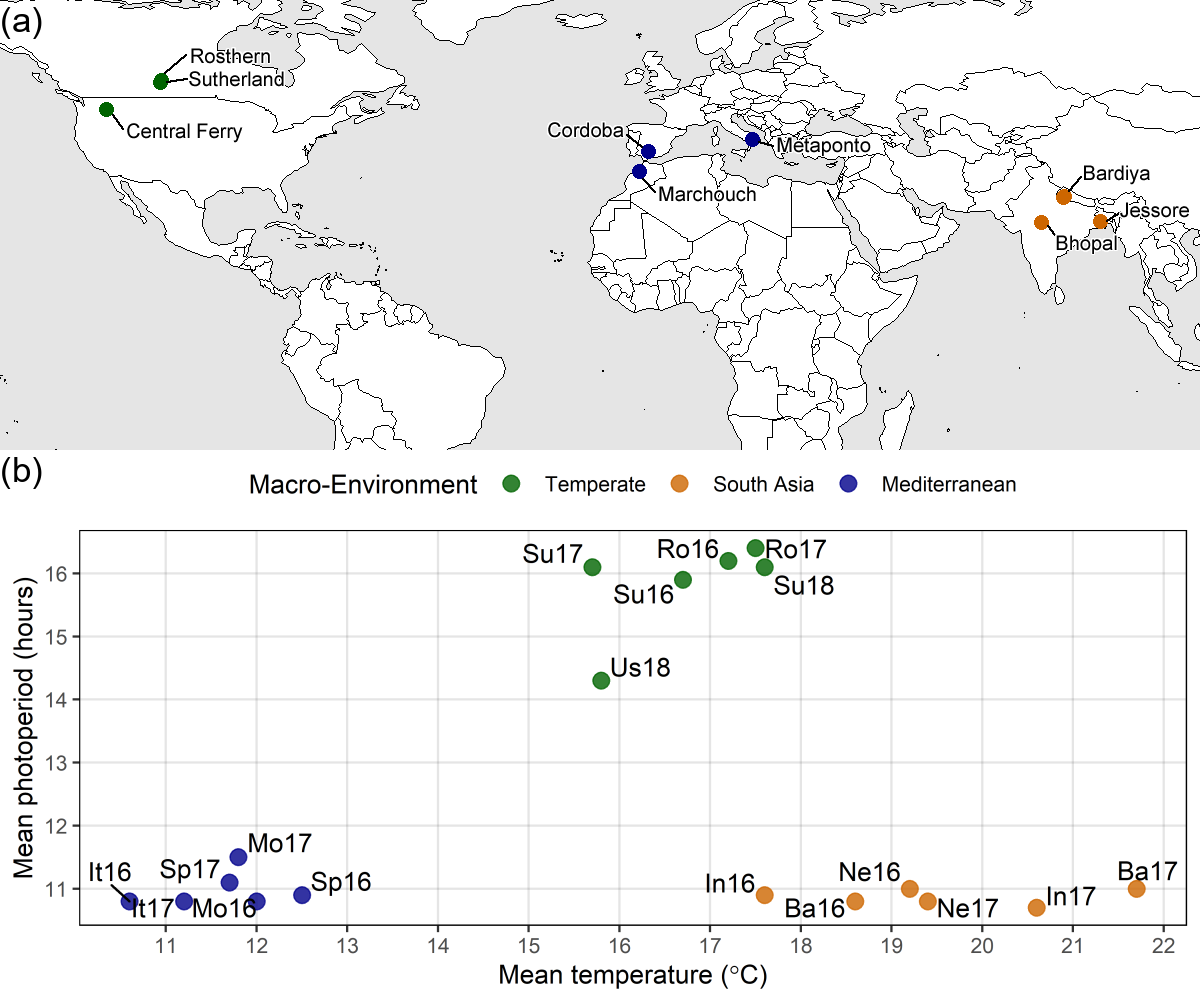
\includegraphics{Figure_01.png}

\begin{Shaded}
\begin{Highlighting}[]
\CommentTok{# Prep data}
\NormalTok{xx <-}\StringTok{ }\NormalTok{ff }\OperatorTok\StringTok{ }\KeywordTok{mutate}\NormalTok{(}\DataTypeTok{Size =} \DecValTok{1}\NormalTok{)}
\CommentTok{# Plot (a) Map}
\KeywordTok{invisible}\NormalTok{(}\KeywordTok{png}\NormalTok{(}\StringTok{"Additional/Temp/Temp_F01_1.png"}\NormalTok{, }\DataTypeTok{width =} \DecValTok{4200}\NormalTok{, }\DataTypeTok{height =} \DecValTok{1575}\NormalTok{, }\DataTypeTok{res =} \DecValTok{600}\NormalTok{))}
\KeywordTok{par}\NormalTok{(}\DataTypeTok{mai =} \KeywordTok{c}\NormalTok{(}\DecValTok{0}\NormalTok{,}\DecValTok{0}\NormalTok{,}\DecValTok{0}\NormalTok{,}\DecValTok{0}\NormalTok{), }\DataTypeTok{xaxs =} \StringTok{"i"}\NormalTok{, }\DataTypeTok{yaxs =} \StringTok{"i"}\NormalTok{)}
\KeywordTok{mapBubbles}\NormalTok{(}\DataTypeTok{dF =}\NormalTok{ xx, }\DataTypeTok{nameX =} \StringTok{"Lon"}\NormalTok{, }\DataTypeTok{nameY =} \StringTok{"Lat"}\NormalTok{, }\DataTypeTok{nameZColour =} \StringTok{"MacroEnv"}\NormalTok{,}
           \DataTypeTok{nameZSize =} \StringTok{"Size"}\NormalTok{, }\DataTypeTok{symbolSize =} \FloatTok{0.5}\NormalTok{, }\DataTypeTok{pch =} \DecValTok{20}\NormalTok{, }\DataTypeTok{fill =}\NormalTok{ F, }\DataTypeTok{addLegend =}\NormalTok{ F,}
           \DataTypeTok{colourPalette =} \KeywordTok{c}\NormalTok{(}\StringTok{"darkgreen"}\NormalTok{, }\StringTok{"darkorange3"}\NormalTok{, }\StringTok{"darkblue"}\NormalTok{), }\DataTypeTok{addColourLegend =}\NormalTok{ F, }
           \DataTypeTok{xlim =} \KeywordTok{c}\NormalTok{(}\OperatorTok{-}\DecValTok{140}\NormalTok{,}\DecValTok{110}\NormalTok{), }\DataTypeTok{ylim =} \KeywordTok{c}\NormalTok{(}\DecValTok{10}\NormalTok{,}\DecValTok{35}\NormalTok{),  }
           \DataTypeTok{oceanCol =} \StringTok{"grey90"}\NormalTok{, }\DataTypeTok{landCol =} \StringTok{"white"}\NormalTok{, }\DataTypeTok{borderCol =} \StringTok{"black"}\NormalTok{)}
\KeywordTok{invisible}\NormalTok{(}\KeywordTok{dev.off}\NormalTok{())}
\CommentTok{# Plot (b) mean T and P}
\NormalTok{mp <-}\StringTok{ }\KeywordTok{ggplot}\NormalTok{(ff, }\KeywordTok{aes}\NormalTok{(}\DataTypeTok{x =}\NormalTok{ T_mean, }\DataTypeTok{y =}\NormalTok{ P_mean)) }\OperatorTok{+}\StringTok{ }
\StringTok{  }\KeywordTok{geom_point}\NormalTok{(}\KeywordTok{aes}\NormalTok{(}\DataTypeTok{color =}\NormalTok{ MacroEnv), }\DataTypeTok{size =} \DecValTok{3}\NormalTok{, }\DataTypeTok{alpha =} \FloatTok{0.8}\NormalTok{) }\OperatorTok{+}\StringTok{ }
\StringTok{  }\KeywordTok{geom_text_repel}\NormalTok{(}\KeywordTok{aes}\NormalTok{(}\DataTypeTok{label =}\NormalTok{ ExptShort)) }\OperatorTok{+}\StringTok{ }
\StringTok{  }\KeywordTok{scale_x_continuous}\NormalTok{(}\DataTypeTok{breaks =} \DecValTok{11}\OperatorTok{:}\DecValTok{22}\NormalTok{) }\OperatorTok{+}
\StringTok{  }\KeywordTok{scale_y_continuous}\NormalTok{(}\DataTypeTok{breaks =} \DecValTok{11}\OperatorTok{:}\DecValTok{16}\NormalTok{) }\OperatorTok{+}
\StringTok{  }\KeywordTok{scale_color_manual}\NormalTok{(}\DataTypeTok{name =} \StringTok{"Macro-Environment"}\NormalTok{,}
                     \DataTypeTok{values =} \KeywordTok{c}\NormalTok{(}\StringTok{"darkgreen"}\NormalTok{,}\StringTok{"darkorange3"}\NormalTok{,}\StringTok{"darkblue"}\NormalTok{)) }\OperatorTok{+}
\StringTok{  }\NormalTok{theme_AGL }\OperatorTok{+}\StringTok{ }
\StringTok{  }\KeywordTok{theme}\NormalTok{(}\DataTypeTok{legend.position =} \StringTok{"top"}\NormalTok{, }\DataTypeTok{legend.margin =} \KeywordTok{unit}\NormalTok{(}\KeywordTok{c}\NormalTok{(}\DecValTok{0}\NormalTok{,}\DecValTok{0}\NormalTok{,}\DecValTok{0}\NormalTok{,}\DecValTok{0}\NormalTok{), }\StringTok{"cm"}\NormalTok{)) }\OperatorTok{+}
\StringTok{  }\KeywordTok{labs}\NormalTok{(}\DataTypeTok{x =} \KeywordTok{expression}\NormalTok{(}\KeywordTok{paste}\NormalTok{(}\StringTok{"Mean temperature ("}\NormalTok{, degree, }\StringTok{"C)"}\NormalTok{, }\DataTypeTok{sep =} \StringTok{""}\NormalTok{)), }
       \DataTypeTok{y =} \StringTok{"Mean photoperiod (h)"}\NormalTok{)}
\KeywordTok{ggsave}\NormalTok{(}\StringTok{"Additional/Temp/Temp_F01_2.png"}\NormalTok{, mp, }\DataTypeTok{width =} \DecValTok{7}\NormalTok{, }\DataTypeTok{height =} \FloatTok{3.25}\NormalTok{, }\DataTypeTok{dpi =} \DecValTok{600}\NormalTok{)}
\CommentTok{# Labels were added to "Additional/Temp/Temp_F1_1.png" in image editing software}
\CommentTok{# Append (a) and (b)}
\NormalTok{im1 <-}\StringTok{ }\KeywordTok{image_read}\NormalTok{(}\StringTok{"Additional/Temp/Temp_F01_1_1.png"}\NormalTok{) }\OperatorTok\StringTok{ }
\StringTok{  }\KeywordTok{image_annotate}\NormalTok{(}\StringTok{"(a)"}\NormalTok{, }\DataTypeTok{size =} \DecValTok{35}\NormalTok{)}
\NormalTok{im2 <-}\StringTok{ }\KeywordTok{image_read}\NormalTok{(}\StringTok{"Additional/Temp/Temp_F01_2.png"}\NormalTok{) }\OperatorTok\StringTok{ }\KeywordTok{image_scale}\NormalTok{(}\StringTok{"1200x"}\NormalTok{) }\OperatorTok
\StringTok{  }\KeywordTok{image_annotate}\NormalTok{(}\StringTok{"(b)"}\NormalTok{, }\DataTypeTok{size =} \DecValTok{35}\NormalTok{)}
\NormalTok{im <-}\StringTok{ }\KeywordTok{image_append}\NormalTok{(}\KeywordTok{c}\NormalTok{(im1, im2), }\DataTypeTok{stack =}\NormalTok{ T)}
\KeywordTok{image_write}\NormalTok{(im, }\StringTok{"Figure_01.png"}\NormalTok{)}
\end{Highlighting}
\end{Shaded}

\hypertarget{additional-figure-1-ldp-origin-map}{%
\subsection{Additional Figure 1 LDP Origin
Map}\label{additional-figure-1-ldp-origin-map}}

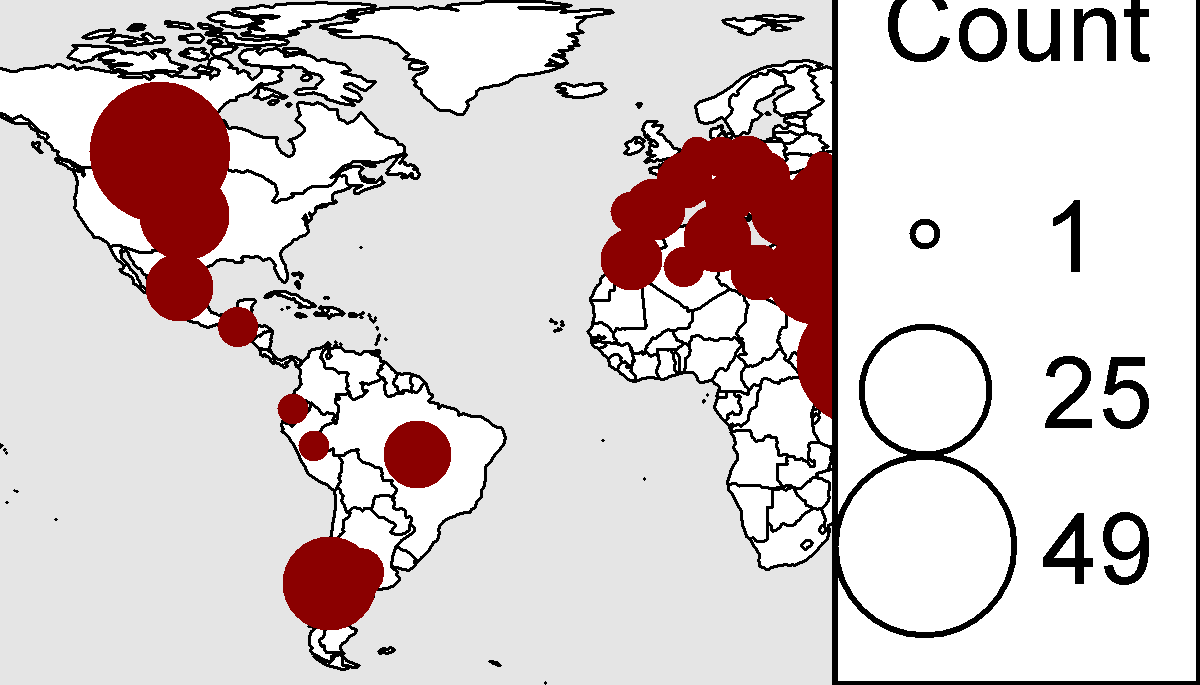
\includegraphics{Additional/Additional_Figure_01.png}

\begin{Shaded}
\begin{Highlighting}[]
\CommentTok{# Prep data}
\NormalTok{x1 <-}\StringTok{ }\NormalTok{ldp }\OperatorTok\StringTok{ }\KeywordTok{filter}\NormalTok{(Origin }\OperatorTok{!=}\StringTok{ "Unknown"}\NormalTok{) }\OperatorTok
\StringTok{  }\KeywordTok{mutate}\NormalTok{(}\DataTypeTok{Origin =} \KeywordTok{recode}\NormalTok{(Origin, }\StringTok{"ICARDA"}\NormalTok{=}\StringTok{"Syria"}\NormalTok{, }\StringTok{"USDA"}\NormalTok{=}\StringTok{"USA"}\NormalTok{)) }\OperatorTok\StringTok{ }
\StringTok{  }\KeywordTok{group_by}\NormalTok{(Origin) }\OperatorTok\StringTok{ }\KeywordTok{summarise}\NormalTok{(}\DataTypeTok{Count =} \KeywordTok{n}\NormalTok{()) }\OperatorTok\StringTok{ }
\StringTok{  }\KeywordTok{left_join}\NormalTok{(}\KeywordTok{select}\NormalTok{(ct, }\DataTypeTok{Origin =}\NormalTok{ Country, Lat, Lon), }\DataTypeTok{by =} \StringTok{"Origin"}\NormalTok{) }\OperatorTok\StringTok{ }
\StringTok{  }\KeywordTok{ungroup}\NormalTok{() }\OperatorTok\StringTok{ }\KeywordTok{as.data.frame}\NormalTok{()}
\NormalTok{x1[}\KeywordTok{is.na}\NormalTok{(x1)] <-}\StringTok{ }\DecValTok{0}
\CommentTok{# Plot}
\KeywordTok{invisible}\NormalTok{(}\KeywordTok{png}\NormalTok{(}\StringTok{"Additional/Additional_Figure_01.png"}\NormalTok{, }
              \DataTypeTok{width =} \DecValTok{3600}\NormalTok{, }\DataTypeTok{height =} \DecValTok{2055}\NormalTok{, }\DataTypeTok{res =} \DecValTok{600}\NormalTok{)) }\CommentTok{#res = 150}
\KeywordTok{par}\NormalTok{(}\DataTypeTok{mai =} \KeywordTok{c}\NormalTok{(}\DecValTok{0}\NormalTok{,}\DecValTok{0}\NormalTok{,}\DecValTok{0}\NormalTok{,}\DecValTok{0}\NormalTok{), }\DataTypeTok{xaxs =} \StringTok{"i"}\NormalTok{,}\DataTypeTok{yaxs =} \StringTok{"i"}\NormalTok{)}
\KeywordTok{mapBubbles}\NormalTok{(}\DataTypeTok{dF =}\NormalTok{ x1, }\DataTypeTok{nameX =} \StringTok{"Lon"}\NormalTok{, }\DataTypeTok{nameY =} \StringTok{"Lat"}\NormalTok{, }
        \DataTypeTok{nameZSize =} \StringTok{"Count"}\NormalTok{, }\DataTypeTok{nameZColour =} \StringTok{"darkred"}\NormalTok{,}
        \DataTypeTok{xlim =} \KeywordTok{c}\NormalTok{(}\OperatorTok{-}\DecValTok{140}\NormalTok{,}\DecValTok{110}\NormalTok{), }\DataTypeTok{ylim =} \KeywordTok{c}\NormalTok{(}\DecValTok{5}\NormalTok{,}\DecValTok{20}\NormalTok{),}
        \DataTypeTok{oceanCol =} \StringTok{"grey90"}\NormalTok{, }\DataTypeTok{landCol =} \StringTok{"white"}\NormalTok{, }\DataTypeTok{borderCol =} \StringTok{"black"}\NormalTok{)}
\KeywordTok{invisible}\NormalTok{(}\KeywordTok{dev.off}\NormalTok{())}
\end{Highlighting}
\end{Shaded}

\hypertarget{supplemental-figure-1-scaling}{%
\subsection{Supplemental Figure 1
Scaling}\label{supplemental-figure-1-scaling}}

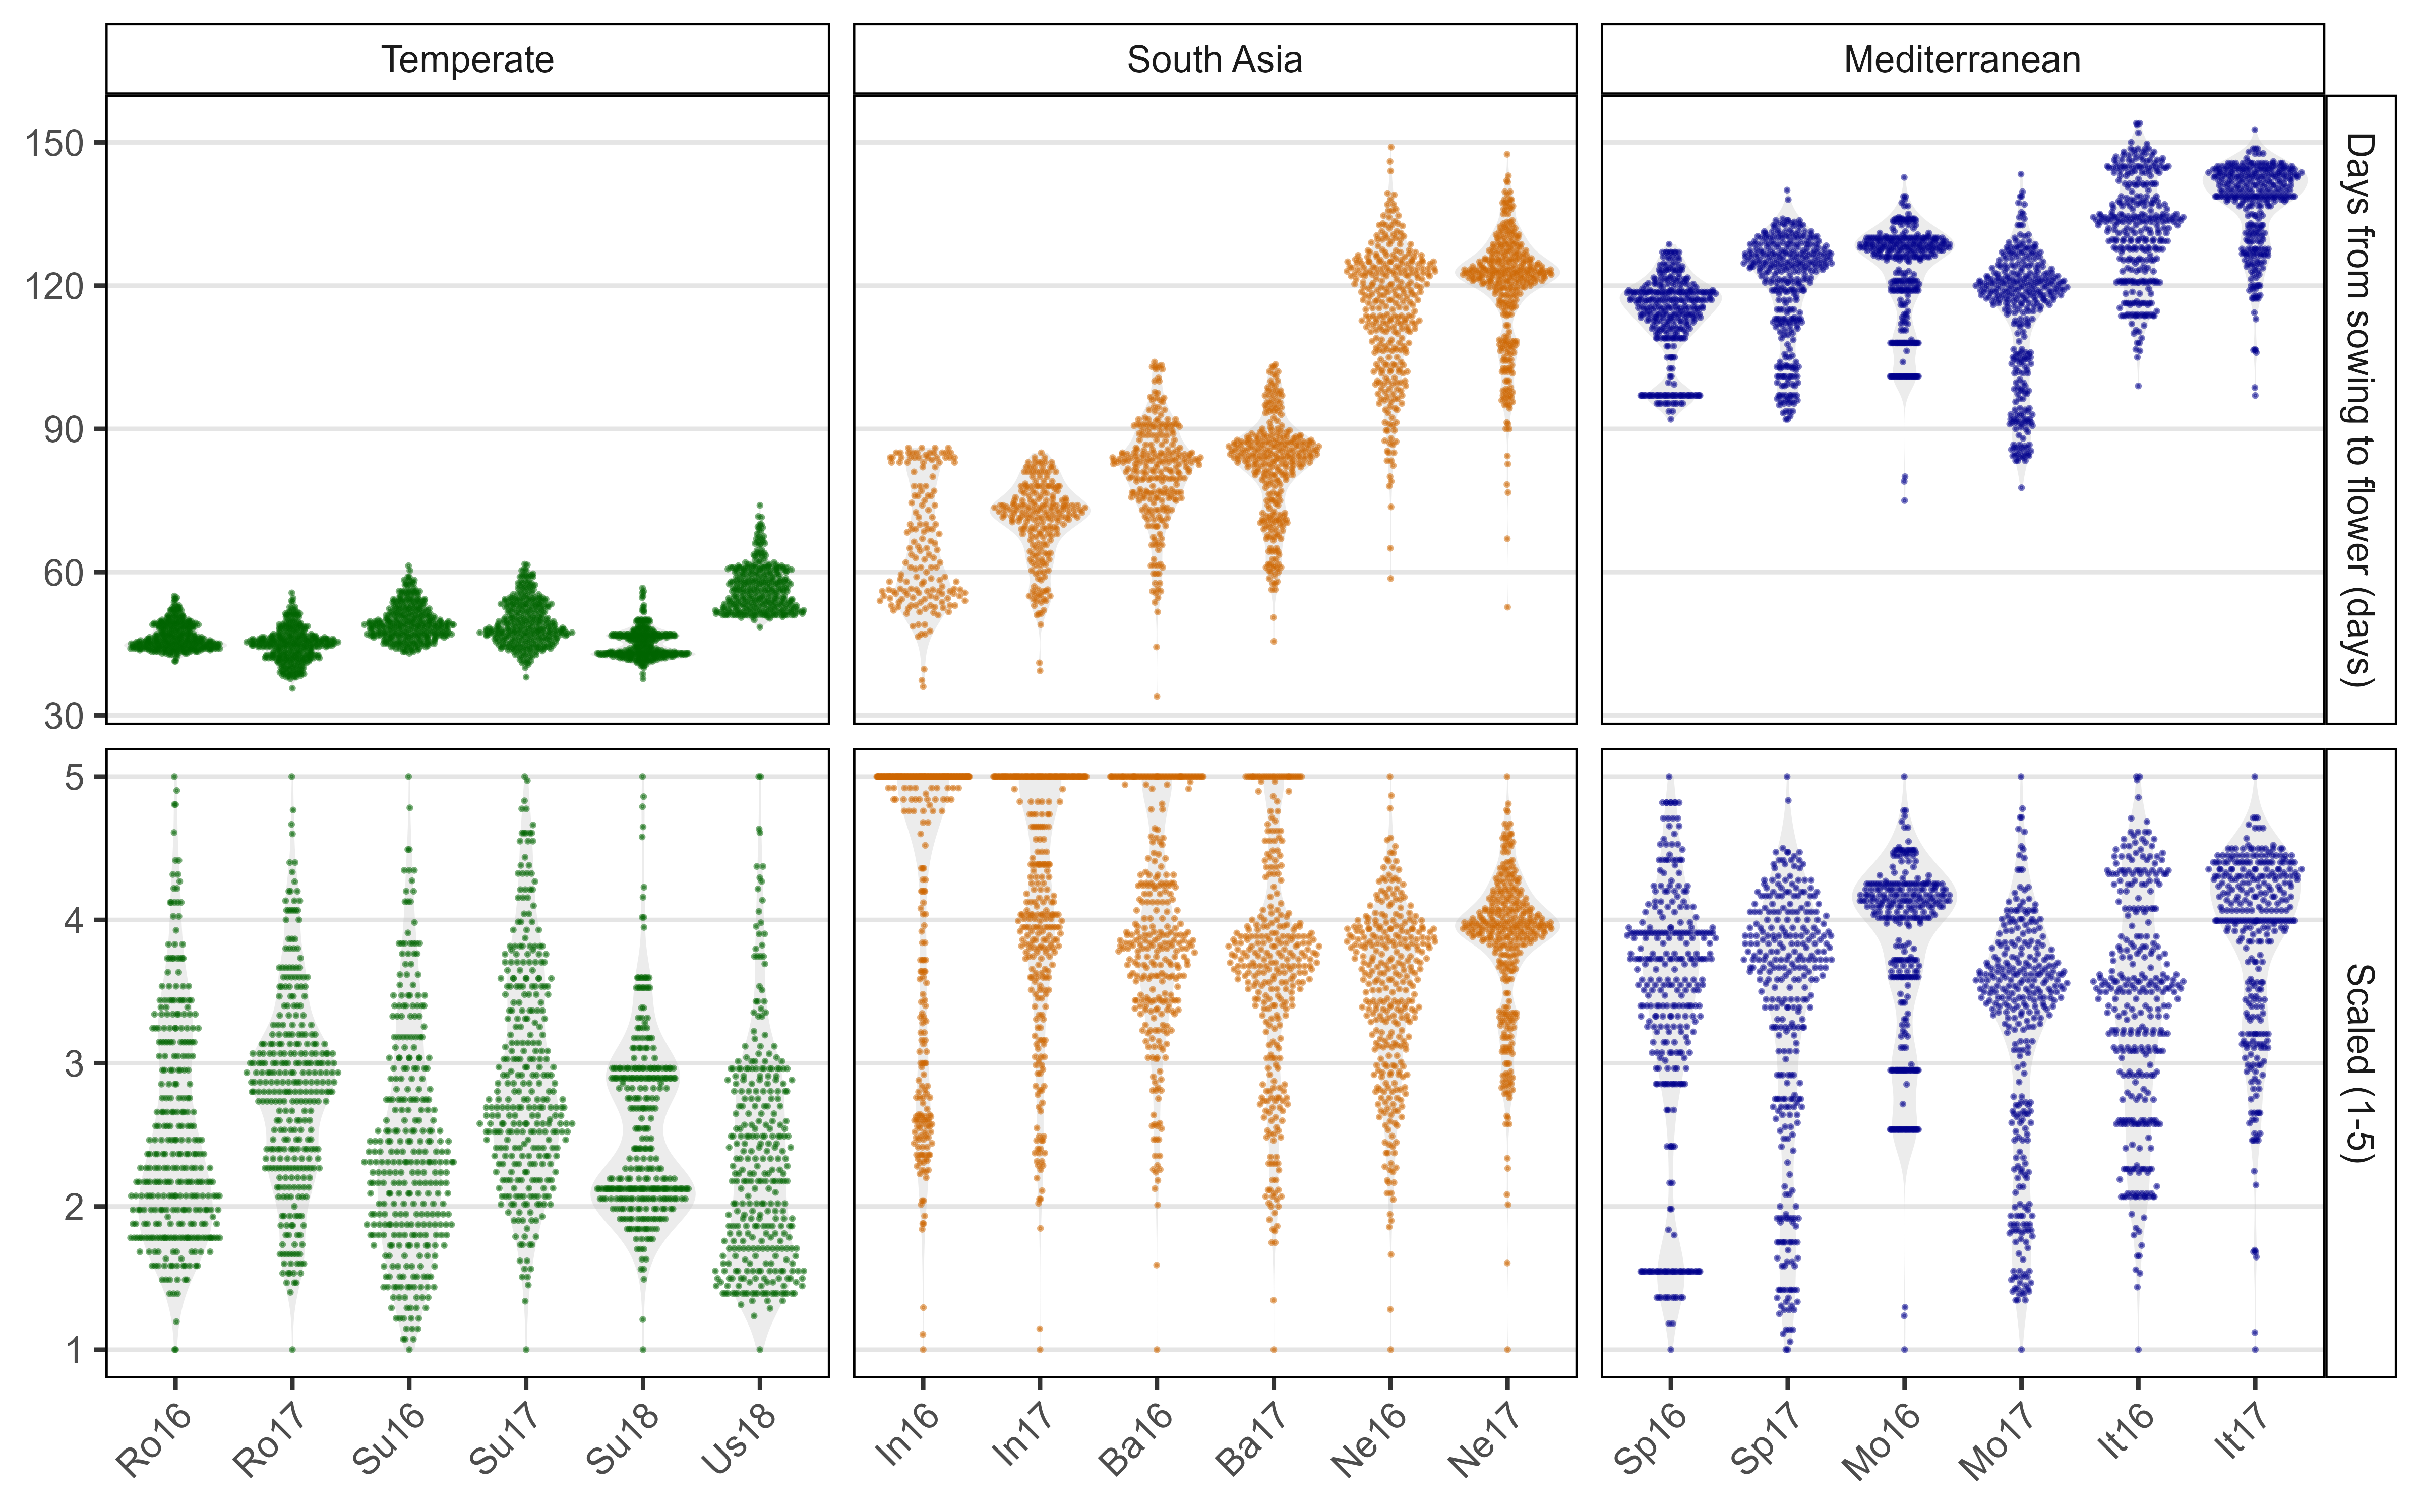
\includegraphics{Supplemental_Figure_01.png}

\begin{Shaded}
\begin{Highlighting}[]
\CommentTok{# Prep data}
\NormalTok{levs <-}\StringTok{ }\KeywordTok{c}\NormalTok{(}\StringTok{"Days from sowing to flower (days)"}\NormalTok{, }\StringTok{"Scaled (1-5)"}\NormalTok{)}
\NormalTok{xx <-}\StringTok{ }\NormalTok{dd }\OperatorTok\StringTok{ }\KeywordTok{select}\NormalTok{(Entry, Expt, ExptShort, DTF, DTF2_scaled) }\OperatorTok
\StringTok{  }\KeywordTok{left_join}\NormalTok{(}\KeywordTok{select}\NormalTok{(ff, Expt, MacroEnv), }\DataTypeTok{by =} \StringTok{"Expt"}\NormalTok{) }\OperatorTok
\StringTok{  }\KeywordTok{gather}\NormalTok{(Trait, Value, DTF, DTF2_scaled) }\OperatorTok\StringTok{ }
\StringTok{  }\KeywordTok{mutate}\NormalTok{(}\DataTypeTok{Trait =}\NormalTok{ plyr}\OperatorTok{::}\KeywordTok{mapvalues}\NormalTok{(Trait, }\KeywordTok{c}\NormalTok{(}\StringTok{"DTF"}\NormalTok{, }\StringTok{"DTF2_scaled"}\NormalTok{), levs),}
         \DataTypeTok{Trait =} \KeywordTok{factor}\NormalTok{(Trait, }\DataTypeTok{levels =}\NormalTok{ levs) )}
\CommentTok{# Plot}
\NormalTok{mp <-}\StringTok{ }\KeywordTok{ggplot}\NormalTok{(xx, }\KeywordTok{aes}\NormalTok{(}\DataTypeTok{x =}\NormalTok{ ExptShort, }\DataTypeTok{y =}\NormalTok{ Value)) }\OperatorTok{+}\StringTok{ }
\StringTok{  }\KeywordTok{geom_violin}\NormalTok{(}\DataTypeTok{fill =} \StringTok{"grey"}\NormalTok{, }\DataTypeTok{alpha =} \FloatTok{0.3}\NormalTok{, }\DataTypeTok{color =} \OtherTok{NA}\NormalTok{) }\OperatorTok{+}\StringTok{ }
\StringTok{  }\KeywordTok{geom_quasirandom}\NormalTok{(}\KeywordTok{aes}\NormalTok{(}\DataTypeTok{color =}\NormalTok{ MacroEnv), }\DataTypeTok{size =} \FloatTok{0.1}\NormalTok{, }\DataTypeTok{alpha =} \FloatTok{0.5}\NormalTok{) }\OperatorTok{+}
\StringTok{  }\KeywordTok{scale_color_manual}\NormalTok{(}\DataTypeTok{values =} \KeywordTok{c}\NormalTok{(}\StringTok{"darkgreen"}\NormalTok{,}\StringTok{"darkorange3"}\NormalTok{,}\StringTok{"darkblue"}\NormalTok{)) }\OperatorTok{+}
\StringTok{  }\KeywordTok{facet_grid}\NormalTok{(Trait }\OperatorTok{~}\StringTok{ }\NormalTok{MacroEnv, }\DataTypeTok{scales =} \StringTok{"free"}\NormalTok{) }\OperatorTok{+}\StringTok{ }
\StringTok{  }\NormalTok{theme_AGL }\OperatorTok{+}\StringTok{ }
\StringTok{  }\KeywordTok{theme}\NormalTok{(}\DataTypeTok{legend.position =} \StringTok{"none"}\NormalTok{,}
        \DataTypeTok{panel.grid.major.x =} \KeywordTok{element_blank}\NormalTok{(),}
        \DataTypeTok{axis.text.x =} \KeywordTok{element_text}\NormalTok{(}\DataTypeTok{angle =} \DecValTok{90}\NormalTok{, }\DataTypeTok{vjust =} \FloatTok{0.5}\NormalTok{, }\DataTypeTok{hjust =} \DecValTok{1}\NormalTok{)) }\OperatorTok{+}
\StringTok{  }\KeywordTok{labs}\NormalTok{(}\DataTypeTok{x =} \OtherTok{NULL}\NormalTok{, }\DataTypeTok{y =} \OtherTok{NULL}\NormalTok{)}
\KeywordTok{ggsave}\NormalTok{(}\StringTok{"Supplemental_Figure_01.png"}\NormalTok{, mp, }\DataTypeTok{width =} \DecValTok{8}\NormalTok{, }\DataTypeTok{height =} \DecValTok{5}\NormalTok{, }\DataTypeTok{dpi =} \DecValTok{600}\NormalTok{)}
\end{Highlighting}
\end{Shaded}

\hypertarget{phenology}{%
\section{Phenology}\label{phenology}}

\hypertarget{figure-2-data-overview}{%
\subsection{Figure 2 Data Overview}\label{figure-2-data-overview}}

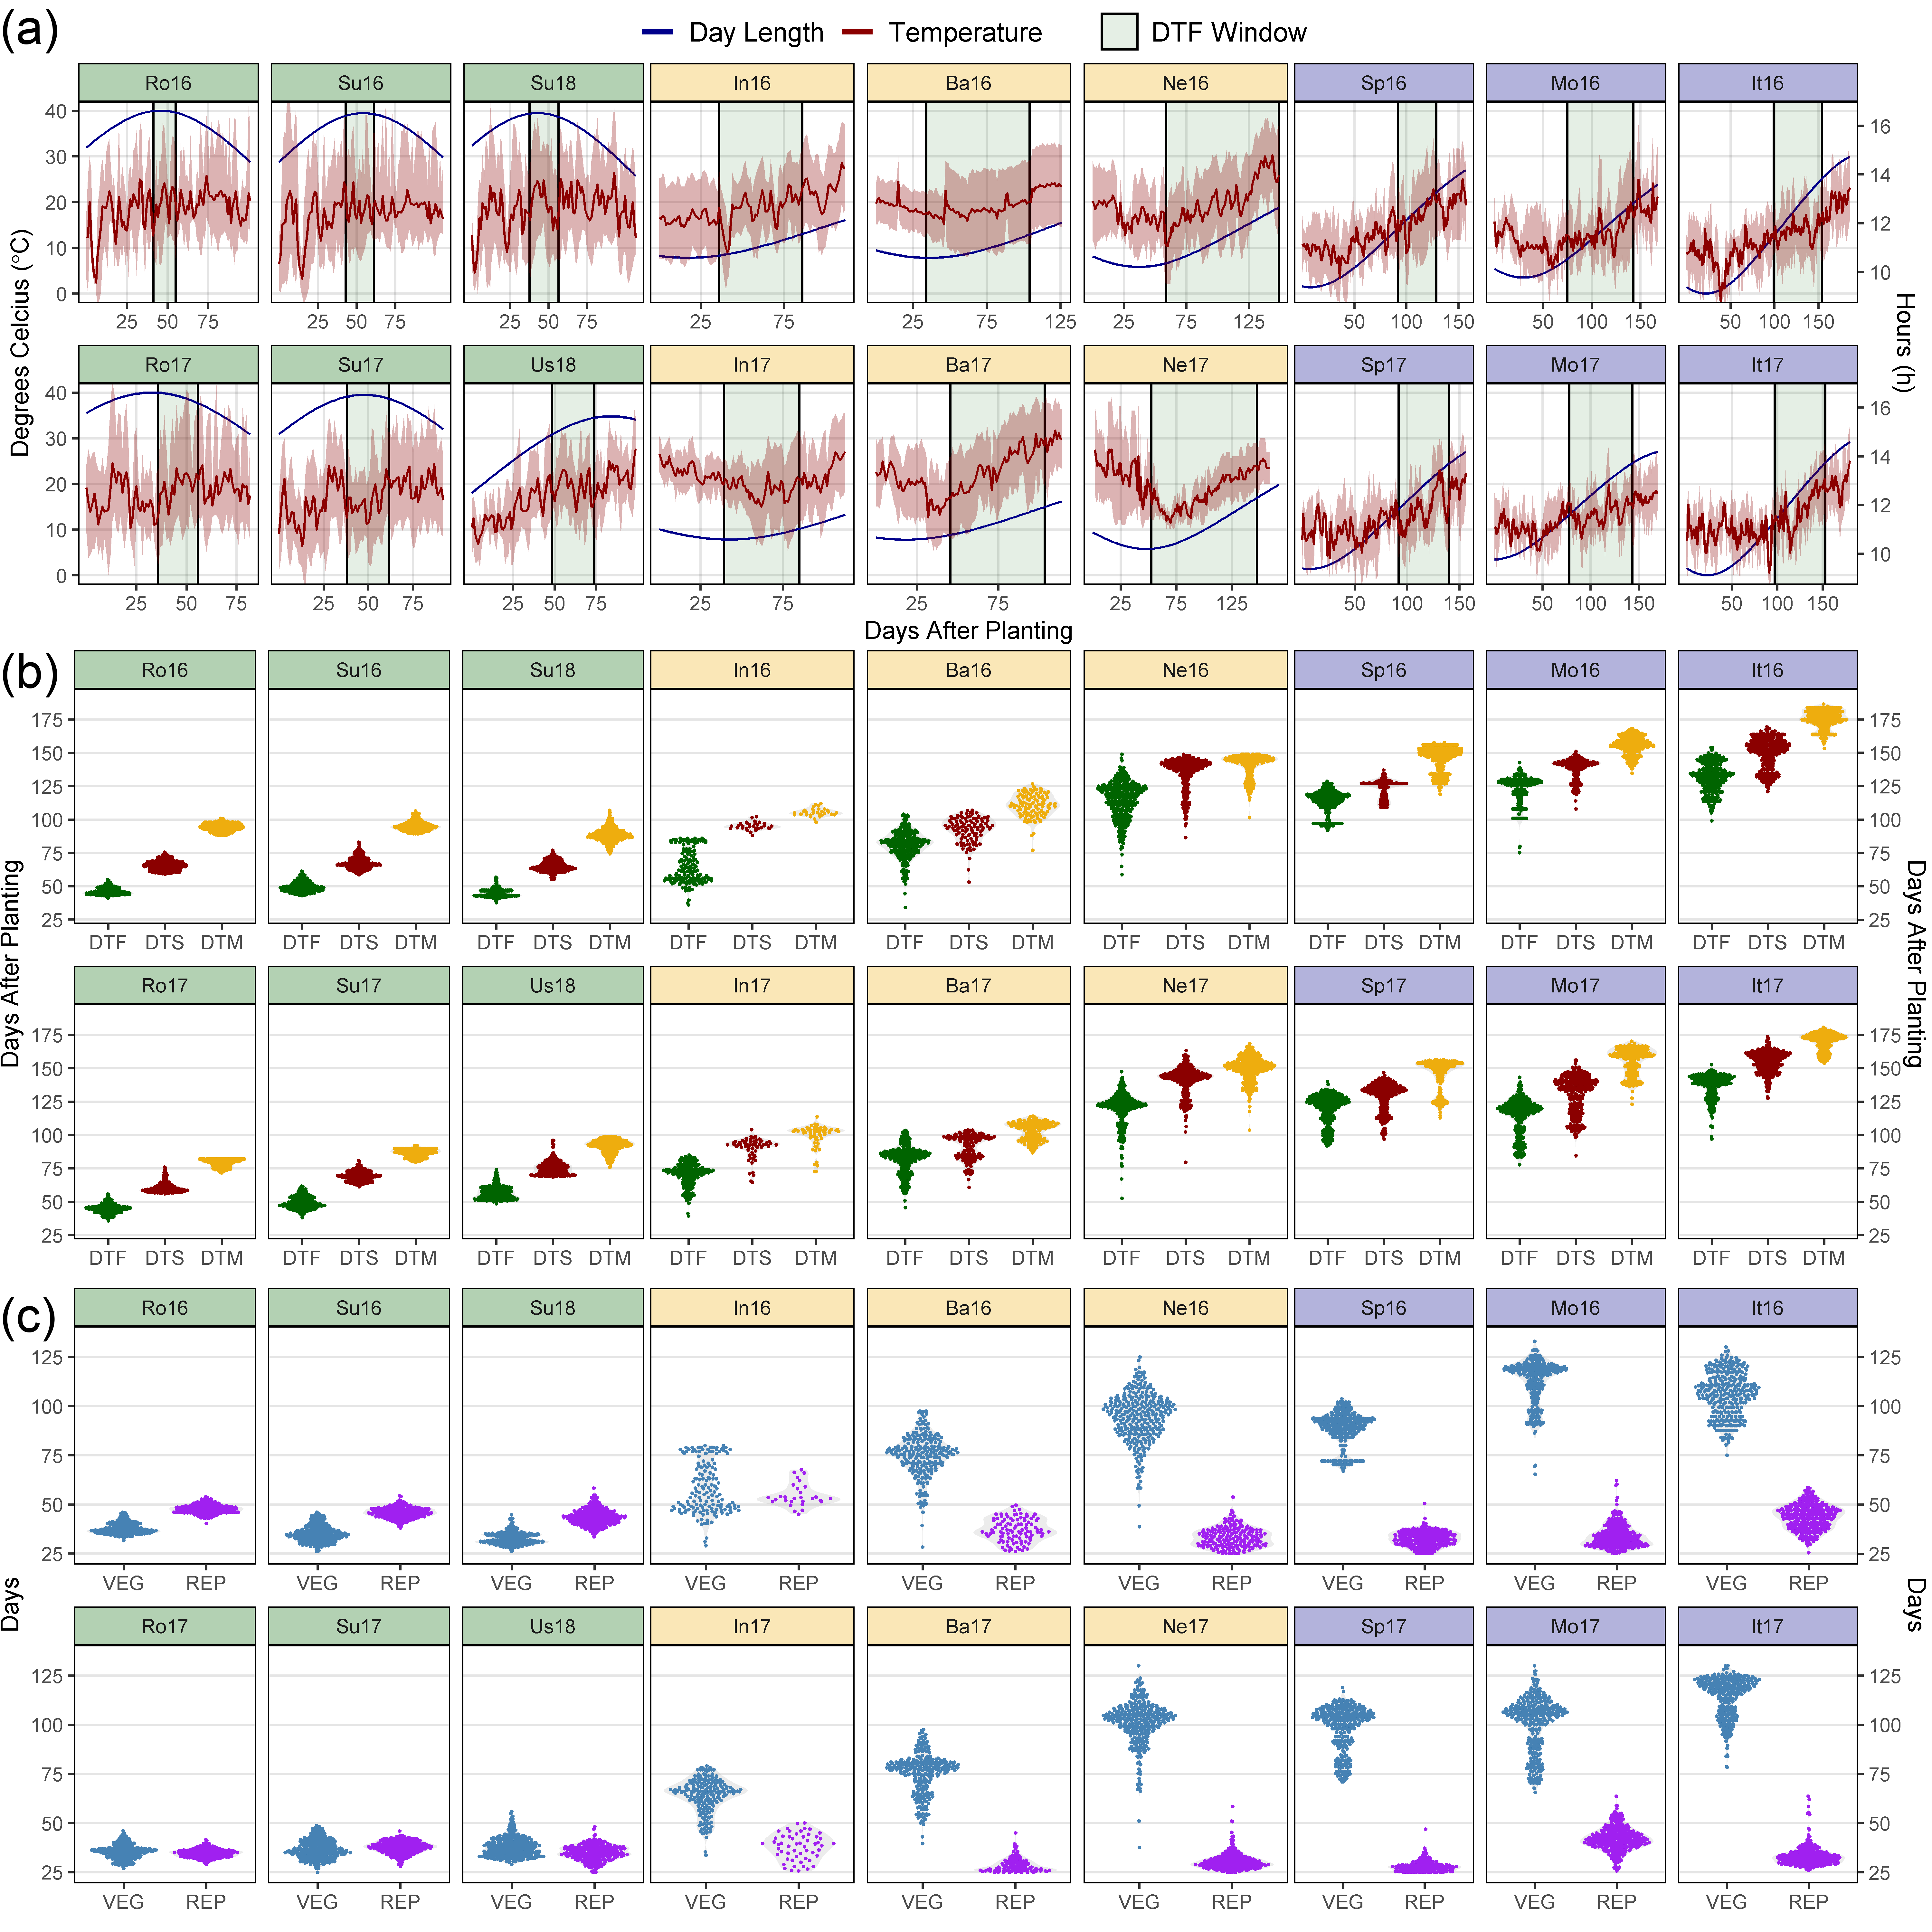
\includegraphics{Figure_02.png}

\begin{Shaded}
\begin{Highlighting}[]
\CommentTok{# Create plot function}
\NormalTok{ggEnvPlot <-}\StringTok{ }\ControlFlowTok{function}\NormalTok{(x, }\DataTypeTok{nr =} \DecValTok{2}\NormalTok{, }\DataTypeTok{nc =} \DecValTok{3}\NormalTok{, mybreaks) \{}
\NormalTok{  yy <-}\StringTok{ }\NormalTok{ff }\OperatorTok\StringTok{ }\KeywordTok{filter}\NormalTok{(Expt }\OperatorTok\StringTok{ }\KeywordTok{unique}\NormalTok{(x}\OperatorTok{$}\NormalTok{Expt)) }\OperatorTok\StringTok{ }
\StringTok{    }\KeywordTok{select}\NormalTok{(ExptShort, Location, Year, }\DataTypeTok{min=}\NormalTok{DTF_min, }\DataTypeTok{max=}\NormalTok{DTF_max) }\OperatorTok
\StringTok{    }\KeywordTok{mutate}\NormalTok{(}\DataTypeTok{Trait =} \StringTok{"DTF Window"}\NormalTok{)}
  \KeywordTok{ggplot}\NormalTok{(x) }\OperatorTok{+}
\StringTok{    }\KeywordTok{geom_rect}\NormalTok{(}\DataTypeTok{data =}\NormalTok{ yy, }\KeywordTok{aes}\NormalTok{(}\DataTypeTok{xmin =}\NormalTok{ min, }\DataTypeTok{xmax =}\NormalTok{ max, }\DataTypeTok{fill =}\NormalTok{ Trait),   }
              \DataTypeTok{ymin =} \OperatorTok{-}\OtherTok{Inf}\NormalTok{, }\DataTypeTok{ymax =} \OtherTok{Inf}\NormalTok{, }\DataTypeTok{alpha =} \FloatTok{0.1}\NormalTok{, }\DataTypeTok{color =} \StringTok{"black"}\NormalTok{) }\OperatorTok{+}
\StringTok{    }\KeywordTok{geom_line}\NormalTok{(}\KeywordTok{aes}\NormalTok{(}\DataTypeTok{x =}\NormalTok{ DaysAfterPlanting, }\DataTypeTok{y =}\NormalTok{ DayLength_rescaled, }\DataTypeTok{color =} \StringTok{"Day Length"}\NormalTok{)) }\OperatorTok{+}
\StringTok{    }\KeywordTok{geom_line}\NormalTok{(}\KeywordTok{aes}\NormalTok{(}\DataTypeTok{x =}\NormalTok{ DaysAfterPlanting, }\DataTypeTok{y =}\NormalTok{ Temp_mean, }\DataTypeTok{color =} \StringTok{"Temperature"}\NormalTok{) ) }\OperatorTok{+}
\StringTok{    }\KeywordTok{geom_ribbon}\NormalTok{(}\KeywordTok{aes}\NormalTok{(}\DataTypeTok{x =}\NormalTok{ DaysAfterPlanting, }\DataTypeTok{ymin =}\NormalTok{ Temp_min, }\DataTypeTok{ymax =}\NormalTok{ Temp_max),}
                \DataTypeTok{fill =} \StringTok{"darkred"}\NormalTok{, }\DataTypeTok{alpha =} \FloatTok{0.3}\NormalTok{) }\OperatorTok{+}
\StringTok{    }\KeywordTok{facet_wrap}\NormalTok{(ExptShort }\OperatorTok{~}\StringTok{ }\NormalTok{., }\DataTypeTok{scales =} \StringTok{"free_x"}\NormalTok{, }\DataTypeTok{dir =} \StringTok{"v"}\NormalTok{, }\DataTypeTok{nrow =} \DecValTok{2}\NormalTok{, }\DataTypeTok{ncol =} \DecValTok{3}\NormalTok{) }\OperatorTok{+}
\StringTok{    }\KeywordTok{scale_x_continuous}\NormalTok{(}\DataTypeTok{breaks =}\NormalTok{ mybreaks) }\OperatorTok{+}
\StringTok{    }\KeywordTok{scale_color_manual}\NormalTok{(}\DataTypeTok{name =} \OtherTok{NULL}\NormalTok{, }\DataTypeTok{values =} \KeywordTok{c}\NormalTok{(}\StringTok{"darkblue"}\NormalTok{, }\StringTok{"darkred"}\NormalTok{)) }\OperatorTok{+}
\StringTok{    }\KeywordTok{scale_fill_manual}\NormalTok{(}\DataTypeTok{name =} \OtherTok{NULL}\NormalTok{, }\DataTypeTok{values =} \StringTok{"darkgreen"}\NormalTok{) }\OperatorTok{+}
\StringTok{    }\KeywordTok{coord_cartesian}\NormalTok{(}\DataTypeTok{ylim=}\KeywordTok{c}\NormalTok{(}\DecValTok{0}\NormalTok{, }\DecValTok{40}\NormalTok{)) }\OperatorTok{+}
\StringTok{    }\NormalTok{theme_AGL }\OperatorTok{+}\StringTok{ }
\StringTok{    }\KeywordTok{theme}\NormalTok{(}\DataTypeTok{plot.margin =} \KeywordTok{unit}\NormalTok{(}\KeywordTok{c}\NormalTok{(}\DecValTok{0}\NormalTok{,}\DecValTok{0}\NormalTok{,}\DecValTok{0}\NormalTok{,}\DecValTok{0}\NormalTok{), }\StringTok{"cm"}\NormalTok{),}
          \DataTypeTok{legend.text =} \KeywordTok{element_text}\NormalTok{(}\DataTypeTok{size =} \DecValTok{12}\NormalTok{)) }\OperatorTok{+}
\StringTok{    }\KeywordTok{labs}\NormalTok{(}\DataTypeTok{y =} \OtherTok{NULL}\NormalTok{, }\DataTypeTok{x =} \OtherTok{NULL}\NormalTok{) }\OperatorTok{+}
\StringTok{    }\KeywordTok{guides}\NormalTok{(}\DataTypeTok{colour =} \KeywordTok{guide_legend}\NormalTok{(}\DataTypeTok{order =} \DecValTok{1}\NormalTok{, }\DataTypeTok{override.aes =} \KeywordTok{list}\NormalTok{(}\DataTypeTok{size =} \FloatTok{1.25}\NormalTok{)), }
           \DataTypeTok{fill =} \KeywordTok{guide_legend}\NormalTok{(}\DataTypeTok{order =} \DecValTok{2}\NormalTok{))}
\NormalTok{\}}
\CommentTok{# Plot (a) T and P}
\NormalTok{mp1}\FloatTok{.1}\NormalTok{ <-}\StringTok{ }\KeywordTok{ggEnvPlot}\NormalTok{(ee }\OperatorTok\StringTok{ }\KeywordTok{filter}\NormalTok{(MacroEnv }\OperatorTok{==}\StringTok{ "Temperate"}\NormalTok{), }\DataTypeTok{mybreaks =} \KeywordTok{c}\NormalTok{(}\DecValTok{25}\NormalTok{,}\DecValTok{50}\NormalTok{,}\DecValTok{75}\NormalTok{)) }\OperatorTok{+}
\StringTok{  }\KeywordTok{labs}\NormalTok{(}\DataTypeTok{y =} \KeywordTok{expression}\NormalTok{(}\KeywordTok{paste}\NormalTok{(}\StringTok{"Degrees Celcius ("}\NormalTok{, degree, }\StringTok{"C)"}\NormalTok{))) }\OperatorTok{+}\StringTok{ }
\StringTok{  }\KeywordTok{theme}\NormalTok{(}\DataTypeTok{strip.background =} \KeywordTok{element_rect}\NormalTok{(}\KeywordTok{alpha}\NormalTok{(}\StringTok{"darkgreen"}\NormalTok{, }\FloatTok{0.3}\NormalTok{)),}
        \DataTypeTok{plot.margin =} \KeywordTok{unit}\NormalTok{(}\KeywordTok{c}\NormalTok{(}\DecValTok{0}\NormalTok{,}\DecValTok{0}\NormalTok{,}\DecValTok{0}\NormalTok{,}\FloatTok{0.155}\NormalTok{), }\StringTok{"cm"}\NormalTok{))}
\NormalTok{mp1}\FloatTok{.2}\NormalTok{ <-}\StringTok{ }\KeywordTok{ggEnvPlot}\NormalTok{(ee }\OperatorTok\StringTok{ }\KeywordTok{filter}\NormalTok{(MacroEnv }\OperatorTok{==}\StringTok{ "South Asia"}\NormalTok{), }\DataTypeTok{mybreaks =} \KeywordTok{c}\NormalTok{(}\DecValTok{25}\NormalTok{,}\DecValTok{75}\NormalTok{,}\DecValTok{125}\NormalTok{)) }\OperatorTok{+}
\StringTok{  }\KeywordTok{labs}\NormalTok{(}\DataTypeTok{x =} \StringTok{"Days After Planting"}\NormalTok{) }\OperatorTok{+}
\StringTok{  }\KeywordTok{theme}\NormalTok{(}\DataTypeTok{strip.background =} \KeywordTok{element_rect}\NormalTok{(}\DataTypeTok{fill =} \KeywordTok{alpha}\NormalTok{(}\StringTok{"darkgoldenrod2"}\NormalTok{, }\FloatTok{0.3}\NormalTok{)),}
        \DataTypeTok{axis.text.y =} \KeywordTok{element_blank}\NormalTok{(), }
        \DataTypeTok{axis.ticks.y =} \KeywordTok{element_blank}\NormalTok{())}
\NormalTok{mp1}\FloatTok{.3}\NormalTok{ <-}\StringTok{ }\KeywordTok{ggEnvPlot}\NormalTok{(ee }\OperatorTok\StringTok{ }\KeywordTok{filter}\NormalTok{(MacroEnv }\OperatorTok{==}\StringTok{ "Mediterranean"}\NormalTok{), }\DataTypeTok{mybreaks =} \KeywordTok{c}\NormalTok{(}\DecValTok{50}\NormalTok{,}\DecValTok{100}\NormalTok{,}\DecValTok{150}\NormalTok{)) }\OperatorTok{+}
\StringTok{  }\KeywordTok{scale_y_continuous}\NormalTok{(}\DataTypeTok{sec.axis =} \KeywordTok{sec_axis}\NormalTok{(}\OperatorTok{~}\StringTok{ }\NormalTok{(}\FloatTok{16.62} \OperatorTok{-}\StringTok{ }\FloatTok{9.11}\NormalTok{) }\OperatorTok{*}\StringTok{ }\NormalTok{. }\OperatorTok{/}\StringTok{ }\NormalTok{(}\DecValTok{40} \OperatorTok{-}\StringTok{ }\DecValTok{0}\NormalTok{) }\OperatorTok{+}\StringTok{ }\FloatTok{9.11}\NormalTok{,}
                     \DataTypeTok{name =} \StringTok{"Hours (h)"}\NormalTok{, }\DataTypeTok{breaks =} \KeywordTok{c}\NormalTok{(}\DecValTok{10}\NormalTok{, }\DecValTok{12}\NormalTok{, }\DecValTok{14}\NormalTok{, }\DecValTok{16}\NormalTok{))) }\OperatorTok{+}
\StringTok{  }\KeywordTok{theme}\NormalTok{(}\DataTypeTok{strip.background =} \KeywordTok{element_rect}\NormalTok{(}\DataTypeTok{fill =} \KeywordTok{alpha}\NormalTok{(}\StringTok{"darkblue"}\NormalTok{, }\FloatTok{0.3}\NormalTok{)),}
        \DataTypeTok{plot.margin =} \KeywordTok{unit}\NormalTok{(}\KeywordTok{c}\NormalTok{(}\DecValTok{0}\NormalTok{,}\FloatTok{0.17}\NormalTok{,}\DecValTok{0}\NormalTok{,}\DecValTok{0}\NormalTok{), }\StringTok{"cm"}\NormalTok{),}
        \DataTypeTok{axis.text.y.left =} \KeywordTok{element_blank}\NormalTok{(),}
        \DataTypeTok{axis.ticks.y.left =} \KeywordTok{element_blank}\NormalTok{())}
\NormalTok{mp1 <-}\StringTok{ }\KeywordTok{ggarrange}\NormalTok{(mp1}\FloatTok{.1}\NormalTok{, mp1}\FloatTok{.2}\NormalTok{, mp1}\FloatTok{.3}\NormalTok{, }\DataTypeTok{nrow =} \DecValTok{1}\NormalTok{, }\DataTypeTok{ncol =} \DecValTok{3}\NormalTok{, }\DataTypeTok{align =} \StringTok{"h"}\NormalTok{,}
                 \DataTypeTok{legend =} \StringTok{"top"}\NormalTok{, }\DataTypeTok{common.legend =}\NormalTok{ T)}
\CommentTok{# Prep data}
\NormalTok{xx <-}\StringTok{ }\NormalTok{dd }\OperatorTok\StringTok{ }\KeywordTok{select}\NormalTok{(Entry, Year, Expt, ExptShort, Location, DTF, DTS, DTM) }\OperatorTok
\StringTok{  }\KeywordTok{left_join}\NormalTok{(}\KeywordTok{select}\NormalTok{(ff, Expt, MacroEnv), }\DataTypeTok{by =} \StringTok{"Expt"}\NormalTok{) }\OperatorTok
\StringTok{  }\KeywordTok{gather}\NormalTok{(Trait, Value, DTF, DTS, DTM) }\OperatorTok
\StringTok{  }\KeywordTok{mutate}\NormalTok{(}\DataTypeTok{Trait =} \KeywordTok{factor}\NormalTok{(Trait, }\DataTypeTok{levels =} \KeywordTok{c}\NormalTok{(}\StringTok{"DTF"}\NormalTok{, }\StringTok{"DTS"}\NormalTok{, }\StringTok{"DTM"}\NormalTok{)))}
\CommentTok{# Create plot function}
\NormalTok{ggDistroDTF <-}\StringTok{ }\ControlFlowTok{function}\NormalTok{(x) \{}
  \KeywordTok{ggplot}\NormalTok{(x, }\KeywordTok{aes}\NormalTok{(}\DataTypeTok{x =}\NormalTok{ Trait, }\DataTypeTok{y =}\NormalTok{ Value) ) }\OperatorTok{+}
\StringTok{    }\KeywordTok{geom_violin}\NormalTok{(}\DataTypeTok{color =} \OtherTok{NA}\NormalTok{, }\DataTypeTok{fill =} \StringTok{"grey"}\NormalTok{, }\DataTypeTok{alpha =} \FloatTok{0.3}\NormalTok{) }\OperatorTok{+}\StringTok{ }
\StringTok{    }\KeywordTok{geom_quasirandom}\NormalTok{(}\DataTypeTok{size =} \FloatTok{0.3}\NormalTok{, }\KeywordTok{aes}\NormalTok{(}\DataTypeTok{color =}\NormalTok{ Trait)) }\OperatorTok{+}
\StringTok{    }\KeywordTok{facet_wrap}\NormalTok{(ExptShort }\OperatorTok{~}\StringTok{ }\NormalTok{., }\DataTypeTok{scales =} \StringTok{"free_x"}\NormalTok{, }\DataTypeTok{dir =} \StringTok{"v"}\NormalTok{, }\DataTypeTok{ncol =} \DecValTok{3}\NormalTok{, }\DataTypeTok{nrow =} \DecValTok{2}\NormalTok{) }\OperatorTok{+}\StringTok{ }
\StringTok{    }\KeywordTok{scale_color_manual}\NormalTok{(}\DataTypeTok{values =} \KeywordTok{c}\NormalTok{(}\StringTok{"darkgreen"}\NormalTok{, }\StringTok{"darkred"}\NormalTok{, }\StringTok{"darkgoldenrod2"}\NormalTok{)) }\OperatorTok{+}
\StringTok{    }\KeywordTok{scale_y_continuous}\NormalTok{(}\DataTypeTok{limits =} \KeywordTok{c}\NormalTok{(}\DecValTok{30}\NormalTok{,}\DecValTok{190}\NormalTok{), }\DataTypeTok{breaks =} \KeywordTok{c}\NormalTok{(}\DecValTok{25}\NormalTok{,}\DecValTok{50}\NormalTok{,}\DecValTok{75}\NormalTok{,}\DecValTok{100}\NormalTok{,}\DecValTok{125}\NormalTok{,}\DecValTok{150}\NormalTok{,}\DecValTok{175}\NormalTok{)) }\OperatorTok{+}
\StringTok{    }\NormalTok{theme_AGL }\OperatorTok{+}\StringTok{ }\KeywordTok{labs}\NormalTok{(}\DataTypeTok{y =} \OtherTok{NULL}\NormalTok{, }\DataTypeTok{x =} \OtherTok{NULL}\NormalTok{) }\OperatorTok{+}
\StringTok{    }\KeywordTok{theme}\NormalTok{(}\DataTypeTok{plot.margin =} \KeywordTok{unit}\NormalTok{(}\KeywordTok{c}\NormalTok{(}\FloatTok{0.1}\NormalTok{,}\DecValTok{0}\NormalTok{,}\FloatTok{0.3}\NormalTok{,}\DecValTok{0}\NormalTok{), }\StringTok{"cm"}\NormalTok{))}
\NormalTok{\}}
\CommentTok{# Plot (b) DTF, DTS and DTM}
\NormalTok{mp2}\FloatTok{.1}\NormalTok{ <-}\StringTok{ }\KeywordTok{ggDistroDTF}\NormalTok{(xx }\OperatorTok\StringTok{ }\KeywordTok{filter}\NormalTok{(MacroEnv }\OperatorTok{==}\StringTok{ "Temperate"}\NormalTok{)) }\OperatorTok{+}\StringTok{ }
\StringTok{  }\KeywordTok{labs}\NormalTok{(}\DataTypeTok{y =} \StringTok{"Days After Planting"}\NormalTok{) }\OperatorTok{+}\StringTok{ }
\StringTok{  }\KeywordTok{theme}\NormalTok{(}\DataTypeTok{strip.background =} \KeywordTok{element_rect}\NormalTok{(}\DataTypeTok{fill =} \KeywordTok{alpha}\NormalTok{(}\StringTok{"darkgreen"}\NormalTok{, }\FloatTok{0.3}\NormalTok{)),}
        \DataTypeTok{panel.grid.major.x =} \KeywordTok{element_blank}\NormalTok{())}
\NormalTok{mp2}\FloatTok{.2}\NormalTok{ <-}\StringTok{ }\KeywordTok{ggDistroDTF}\NormalTok{(xx }\OperatorTok\StringTok{ }\KeywordTok{filter}\NormalTok{(MacroEnv }\OperatorTok{==}\StringTok{ "South Asia"}\NormalTok{)) }\OperatorTok{+}
\StringTok{  }\KeywordTok{theme}\NormalTok{(}\DataTypeTok{strip.background =} \KeywordTok{element_rect}\NormalTok{(}\DataTypeTok{fill =} \KeywordTok{alpha}\NormalTok{(}\StringTok{"darkgoldenrod2"}\NormalTok{, }\FloatTok{0.3}\NormalTok{)),}
        \DataTypeTok{panel.grid.major.x =} \KeywordTok{element_blank}\NormalTok{(),}
        \DataTypeTok{axis.text.y =} \KeywordTok{element_blank}\NormalTok{(), }
        \DataTypeTok{axis.ticks.y =} \KeywordTok{element_blank}\NormalTok{())}
\NormalTok{mp2}\FloatTok{.3}\NormalTok{ <-}\StringTok{ }\KeywordTok{ggDistroDTF}\NormalTok{(xx }\OperatorTok\StringTok{ }\KeywordTok{filter}\NormalTok{(MacroEnv }\OperatorTok{==}\StringTok{ "Mediterranean"}\NormalTok{)) }\OperatorTok{+}
\StringTok{  }\KeywordTok{scale_y_continuous}\NormalTok{(}\DataTypeTok{limits =} \KeywordTok{c}\NormalTok{(}\DecValTok{30}\NormalTok{,}\DecValTok{190}\NormalTok{), }\DataTypeTok{breaks =} \KeywordTok{c}\NormalTok{(}\DecValTok{25}\NormalTok{,}\DecValTok{50}\NormalTok{,}\DecValTok{75}\NormalTok{,}\DecValTok{100}\NormalTok{,}\DecValTok{125}\NormalTok{,}\DecValTok{150}\NormalTok{,}\DecValTok{175}\NormalTok{),}
                     \DataTypeTok{sec.axis =} \KeywordTok{sec_axis}\NormalTok{(}\OperatorTok{~}\StringTok{ }\NormalTok{., }\DataTypeTok{name =} \StringTok{"Days After Planting"}\NormalTok{,}
                       \DataTypeTok{breaks =} \KeywordTok{c}\NormalTok{(}\DecValTok{25}\NormalTok{,}\DecValTok{50}\NormalTok{,}\DecValTok{75}\NormalTok{,}\DecValTok{100}\NormalTok{,}\DecValTok{125}\NormalTok{,}\DecValTok{150}\NormalTok{,}\DecValTok{175}\NormalTok{))) }\OperatorTok{+}
\StringTok{  }\KeywordTok{theme}\NormalTok{(}\DataTypeTok{strip.background =} \KeywordTok{element_rect}\NormalTok{(}\DataTypeTok{fill =} \KeywordTok{alpha}\NormalTok{(}\StringTok{"darkblue"}\NormalTok{, }\FloatTok{0.3}\NormalTok{)),}
        \DataTypeTok{panel.grid.major.x =} \KeywordTok{element_blank}\NormalTok{(),}
        \DataTypeTok{panel.grid.minor.x =} \KeywordTok{element_line}\NormalTok{(),}
        \DataTypeTok{axis.text.y.left =} \KeywordTok{element_blank}\NormalTok{(),}
        \DataTypeTok{axis.ticks.y.left =} \KeywordTok{element_blank}\NormalTok{())}
\CommentTok{# Append}
\NormalTok{mp2 <-}\StringTok{ }\KeywordTok{ggarrange}\NormalTok{(mp2}\FloatTok{.1}\NormalTok{, mp2}\FloatTok{.2}\NormalTok{, mp2}\FloatTok{.3}\NormalTok{, }\DataTypeTok{nrow =} \DecValTok{1}\NormalTok{, }\DataTypeTok{ncol =} \DecValTok{3}\NormalTok{, }\DataTypeTok{align =} \StringTok{"h"}\NormalTok{, }\DataTypeTok{legend =} \StringTok{"none"}\NormalTok{)}
\CommentTok{# Prep data}
\NormalTok{xx <-}\StringTok{ }\NormalTok{dd }\OperatorTok\StringTok{ }\KeywordTok{select}\NormalTok{(Entry, Name, Expt, ExptShort, Location, Year, VEG, REP) }\OperatorTok
\StringTok{  }\KeywordTok{left_join}\NormalTok{(}\KeywordTok{select}\NormalTok{(ff, Expt, MacroEnv), }\DataTypeTok{by =} \StringTok{"Expt"}\NormalTok{) }\OperatorTok
\StringTok{  }\KeywordTok{gather}\NormalTok{(Trait, Value, VEG, REP) }\OperatorTok\StringTok{ }
\StringTok{  }\KeywordTok{mutate}\NormalTok{(}\DataTypeTok{Trait =} \KeywordTok{factor}\NormalTok{(Trait, }\DataTypeTok{levels =} \KeywordTok{c}\NormalTok{(}\StringTok{"VEG"}\NormalTok{, }\StringTok{"REP"}\NormalTok{)))}
\CommentTok{# Create plot function}
\NormalTok{ggDistroREP <-}\StringTok{ }\ControlFlowTok{function}\NormalTok{(x) \{}
  \KeywordTok{ggplot}\NormalTok{(x, }\KeywordTok{aes}\NormalTok{(}\DataTypeTok{x =}\NormalTok{ Trait, }\DataTypeTok{y =}\NormalTok{ Value)) }\OperatorTok{+}\StringTok{ }
\StringTok{    }\KeywordTok{geom_violin}\NormalTok{(}\DataTypeTok{color =} \OtherTok{NA}\NormalTok{, }\DataTypeTok{fill =} \StringTok{"grey"}\NormalTok{, }\DataTypeTok{alpha =} \FloatTok{0.3}\NormalTok{) }\OperatorTok{+}\StringTok{ }
\StringTok{    }\KeywordTok{geom_quasirandom}\NormalTok{(}\DataTypeTok{size =} \FloatTok{0.3}\NormalTok{, }\KeywordTok{aes}\NormalTok{(}\DataTypeTok{color =}\NormalTok{ Trait)) }\OperatorTok{+}
\StringTok{    }\KeywordTok{facet_wrap}\NormalTok{(ExptShort }\OperatorTok{~}\StringTok{ }\NormalTok{., }\DataTypeTok{scales =} \StringTok{"free_x"}\NormalTok{, }\DataTypeTok{dir =} \StringTok{"v"}\NormalTok{, }\DataTypeTok{ncol =} \DecValTok{3}\NormalTok{, }\DataTypeTok{nrow =} \DecValTok{2}\NormalTok{) }\OperatorTok{+}
\StringTok{    }\KeywordTok{scale_color_manual}\NormalTok{(}\DataTypeTok{values =} \KeywordTok{c}\NormalTok{(}\StringTok{"steelblue"}\NormalTok{, }\StringTok{"purple"}\NormalTok{)) }\OperatorTok{+}
\StringTok{    }\KeywordTok{scale_y_continuous}\NormalTok{(}\DataTypeTok{limits =} \KeywordTok{c}\NormalTok{(}\DecValTok{25}\NormalTok{,}\DecValTok{135}\NormalTok{), }\DataTypeTok{breaks =} \KeywordTok{c}\NormalTok{(}\DecValTok{25}\NormalTok{,}\DecValTok{50}\NormalTok{,}\DecValTok{75}\NormalTok{,}\DecValTok{100}\NormalTok{,}\DecValTok{125}\NormalTok{)) }\OperatorTok{+}
\StringTok{    }\NormalTok{theme_AGL }\OperatorTok{+}\StringTok{ }\KeywordTok{labs}\NormalTok{(}\DataTypeTok{x =} \OtherTok{NULL}\NormalTok{, }\DataTypeTok{y =} \OtherTok{NULL}\NormalTok{) }\OperatorTok{+}\StringTok{ }
\StringTok{    }\KeywordTok{theme}\NormalTok{(}\DataTypeTok{plot.margin =} \KeywordTok{unit}\NormalTok{(}\KeywordTok{c}\NormalTok{(}\DecValTok{0}\NormalTok{,}\DecValTok{0}\NormalTok{,}\FloatTok{0.3}\NormalTok{,}\DecValTok{0}\NormalTok{), }\StringTok{"cm"}\NormalTok{))}
\NormalTok{\}}
\CommentTok{# Plot (c) REP and VEG}
\NormalTok{mp3}\FloatTok{.1}\NormalTok{ <-}\StringTok{ }\KeywordTok{ggDistroREP}\NormalTok{(xx }\OperatorTok\StringTok{ }\KeywordTok{filter}\NormalTok{(MacroEnv }\OperatorTok{==}\StringTok{ "Temperate"}\NormalTok{)) }\OperatorTok{+}\StringTok{ }
\StringTok{  }\KeywordTok{labs}\NormalTok{(}\DataTypeTok{y =} \StringTok{"Days"}\NormalTok{) }\OperatorTok{+}
\StringTok{  }\KeywordTok{theme}\NormalTok{(}\DataTypeTok{strip.background =} \KeywordTok{element_rect}\NormalTok{(}\DataTypeTok{fill =} \KeywordTok{alpha}\NormalTok{(}\StringTok{"darkgreen"}\NormalTok{, }\FloatTok{0.3}\NormalTok{)),}
        \DataTypeTok{panel.grid.major.x =} \KeywordTok{element_blank}\NormalTok{())}
\NormalTok{mp3}\FloatTok{.2}\NormalTok{ <-}\StringTok{ }\KeywordTok{ggDistroREP}\NormalTok{(xx }\OperatorTok\StringTok{ }\KeywordTok{filter}\NormalTok{(MacroEnv }\OperatorTok{==}\StringTok{ "South Asia"}\NormalTok{)) }\OperatorTok{+}\StringTok{ }
\StringTok{  }\KeywordTok{theme}\NormalTok{(}\DataTypeTok{strip.background =} \KeywordTok{element_rect}\NormalTok{(}\DataTypeTok{fill =} \KeywordTok{alpha}\NormalTok{(}\StringTok{"darkgoldenrod2"}\NormalTok{, }\FloatTok{0.3}\NormalTok{)),}
        \DataTypeTok{panel.grid.major.x =} \KeywordTok{element_blank}\NormalTok{(),}
        \DataTypeTok{axis.text.y =} \KeywordTok{element_blank}\NormalTok{(), }
        \DataTypeTok{axis.ticks.y =} \KeywordTok{element_blank}\NormalTok{())}
\NormalTok{mp3}\FloatTok{.3}\NormalTok{ <-}\StringTok{ }\KeywordTok{ggDistroREP}\NormalTok{(xx }\OperatorTok\StringTok{ }\KeywordTok{filter}\NormalTok{(MacroEnv }\OperatorTok{==}\StringTok{ "Mediterranean"}\NormalTok{)) }\OperatorTok{+}
\StringTok{  }\KeywordTok{scale_y_continuous}\NormalTok{(}\DataTypeTok{limits =} \KeywordTok{c}\NormalTok{(}\DecValTok{25}\NormalTok{,}\DecValTok{135}\NormalTok{), }\DataTypeTok{breaks =} \KeywordTok{c}\NormalTok{(}\DecValTok{25}\NormalTok{,}\DecValTok{50}\NormalTok{,}\DecValTok{75}\NormalTok{,}\DecValTok{100}\NormalTok{,}\DecValTok{125}\NormalTok{),}
                     \DataTypeTok{sec.axis =} \KeywordTok{sec_axis}\NormalTok{(}\OperatorTok{~}\StringTok{ }\NormalTok{., }\DataTypeTok{name =} \StringTok{"Days"}\NormalTok{,}
                       \DataTypeTok{breaks =} \KeywordTok{c}\NormalTok{(}\DecValTok{25}\NormalTok{,}\DecValTok{50}\NormalTok{,}\DecValTok{75}\NormalTok{,}\DecValTok{100}\NormalTok{,}\DecValTok{125}\NormalTok{))) }\OperatorTok{+}
\StringTok{  }\KeywordTok{theme}\NormalTok{(}\DataTypeTok{strip.background =} \KeywordTok{element_rect}\NormalTok{(}\DataTypeTok{fill =} \KeywordTok{alpha}\NormalTok{(}\StringTok{"darkblue"}\NormalTok{, }\FloatTok{0.3}\NormalTok{)),}
        \DataTypeTok{panel.grid.major.x =} \KeywordTok{element_blank}\NormalTok{(),}
        \DataTypeTok{axis.text.y.left =} \KeywordTok{element_blank}\NormalTok{(),}
        \DataTypeTok{axis.ticks.y.left =} \KeywordTok{element_blank}\NormalTok{())}
\CommentTok{# Append}
\NormalTok{mp3 <-}\StringTok{ }\KeywordTok{ggarrange}\NormalTok{(mp3}\FloatTok{.1}\NormalTok{, mp3}\FloatTok{.2}\NormalTok{, mp3}\FloatTok{.3}\NormalTok{, }\DataTypeTok{nrow =} \DecValTok{1}\NormalTok{, }\DataTypeTok{ncol =} \DecValTok{3}\NormalTok{, }\DataTypeTok{align =} \StringTok{"h"}\NormalTok{, }\DataTypeTok{legend =} \StringTok{"none"}\NormalTok{)}
\CommentTok{# Save}
\KeywordTok{ggsave}\NormalTok{(}\StringTok{"Additional/Temp/Temp_F02_1.png"}\NormalTok{, mp1, }\DataTypeTok{width =} \DecValTok{12}\NormalTok{, }\DataTypeTok{height =} \DecValTok{4}\NormalTok{, }\DataTypeTok{dpi =} \DecValTok{600}\NormalTok{)}
\KeywordTok{ggsave}\NormalTok{(}\StringTok{"Additional/Temp/Temp_F02_2.png"}\NormalTok{, mp2, }\DataTypeTok{width =} \DecValTok{12}\NormalTok{, }\DataTypeTok{height =} \DecValTok{4}\NormalTok{, }\DataTypeTok{dpi =} \DecValTok{600}\NormalTok{)}
\KeywordTok{ggsave}\NormalTok{(}\StringTok{"Additional/Temp/Temp_F02_3.png"}\NormalTok{, mp3, }\DataTypeTok{width =} \DecValTok{12}\NormalTok{, }\DataTypeTok{height =} \DecValTok{4}\NormalTok{, }\DataTypeTok{dpi =} \DecValTok{600}\NormalTok{)}
\CommentTok{# Append (a), (b) and (c)}
\NormalTok{mp1 <-}\StringTok{ }\KeywordTok{image_read}\NormalTok{(}\StringTok{"Additional/Temp/Temp_F02_1.png"}\NormalTok{)  }\OperatorTok\StringTok{ }
\StringTok{  }\KeywordTok{image_annotate}\NormalTok{(}\StringTok{"(a)"}\NormalTok{, }\DataTypeTok{size =} \DecValTok{150}\NormalTok{)}
\NormalTok{mp2 <-}\StringTok{ }\KeywordTok{image_read}\NormalTok{(}\StringTok{"Additional/Temp/Temp_F02_2.png"}\NormalTok{) }\OperatorTok\StringTok{ }
\StringTok{  }\KeywordTok{image_annotate}\NormalTok{(}\StringTok{"(b)"}\NormalTok{, }\DataTypeTok{size =} \DecValTok{150}\NormalTok{)}
\NormalTok{mp3 <-}\StringTok{ }\KeywordTok{image_read}\NormalTok{(}\StringTok{"Additional/Temp/Temp_F02_3.png"}\NormalTok{) }\OperatorTok\StringTok{ }
\StringTok{  }\KeywordTok{image_annotate}\NormalTok{(}\StringTok{"(c)"}\NormalTok{, }\DataTypeTok{size =} \DecValTok{150}\NormalTok{)}
\NormalTok{mp <-}\StringTok{ }\KeywordTok{image_append}\NormalTok{(}\KeywordTok{c}\NormalTok{(mp1, mp2, mp3), }\DataTypeTok{stack =}\NormalTok{ T)}
\KeywordTok{image_write}\NormalTok{(mp, }\StringTok{"Figure_02.png"}\NormalTok{)}
\end{Highlighting}
\end{Shaded}

\hypertarget{additional-figures---entry-phenology}{%
\subsection{Additional Figures - Entry
Phenology}\label{additional-figures---entry-phenology}}

\begin{Shaded}
\begin{Highlighting}[]
\CommentTok{# Create plotting function}
\NormalTok{gg_phenol <-}\StringTok{ }\ControlFlowTok{function}\NormalTok{(x, xE, colnums) \{}
\NormalTok{  mycols <-}\StringTok{ }\KeywordTok{c}\NormalTok{(}\StringTok{"darkgreen"}\NormalTok{, }\StringTok{"darkorange3"}\NormalTok{, }\StringTok{"darkblue"}\NormalTok{)}
  \KeywordTok{ggplot}\NormalTok{(xE, }\KeywordTok{aes}\NormalTok{(}\DataTypeTok{x =}\NormalTok{ Trait, }\DataTypeTok{y =}\NormalTok{ Value, }\DataTypeTok{group =}\NormalTok{ Entry, }\DataTypeTok{color =}\NormalTok{ MacroEnv)) }\OperatorTok{+}
\StringTok{    }\KeywordTok{geom_line}\NormalTok{(}\DataTypeTok{data =}\NormalTok{ x, }\DataTypeTok{color =} \StringTok{"grey"}\NormalTok{, }\DataTypeTok{alpha =} \FloatTok{0.5}\NormalTok{) }\OperatorTok{+}
\StringTok{    }\KeywordTok{geom_line}\NormalTok{() }\OperatorTok{+}\StringTok{ }\KeywordTok{geom_point}\NormalTok{() }\OperatorTok{+}
\StringTok{    }\KeywordTok{facet_grid}\NormalTok{(MacroEnv }\OperatorTok{~}\StringTok{ }\NormalTok{ExptShort) }\OperatorTok{+}
\StringTok{    }\KeywordTok{scale_color_manual}\NormalTok{(}\DataTypeTok{values =}\NormalTok{ mycols[colnums]) }\OperatorTok{+}
\StringTok{    }\NormalTok{theme_AGL }\OperatorTok{+}\StringTok{ }
\StringTok{    }\KeywordTok{theme}\NormalTok{(}\DataTypeTok{legend.position =} \StringTok{"none"}\NormalTok{, }\DataTypeTok{panel.grid.major.x =} \KeywordTok{element_blank}\NormalTok{()) }\OperatorTok{+}
\StringTok{    }\KeywordTok{ylim}\NormalTok{(}\KeywordTok{c}\NormalTok{(}\KeywordTok{min}\NormalTok{(x}\OperatorTok{$}\NormalTok{Value, }\DataTypeTok{na.rm =}\NormalTok{ T), }\KeywordTok{max}\NormalTok{(x}\OperatorTok{$}\NormalTok{Value, }\DataTypeTok{na.rm =}\NormalTok{ T))) }\OperatorTok{+}
\StringTok{    }\KeywordTok{labs}\NormalTok{(}\DataTypeTok{x =} \OtherTok{NULL}\NormalTok{, }\DataTypeTok{y =} \StringTok{"Days"}\NormalTok{)}
\NormalTok{\}}
\CommentTok{# Prep data}
\NormalTok{xx <-}\StringTok{ }\NormalTok{dd }\OperatorTok\StringTok{ }\KeywordTok{select}\NormalTok{(Entry, Name, ExptShort, DTF, DTS, DTM) }\OperatorTok\StringTok{ }
\StringTok{  }\KeywordTok{left_join}\NormalTok{(}\KeywordTok{select}\NormalTok{(ff, ExptShort, MacroEnv), }\DataTypeTok{by =} \StringTok{"ExptShort"}\NormalTok{) }\OperatorTok
\StringTok{  }\KeywordTok{gather}\NormalTok{(Trait, Value, DTF, DTS, DTM) }\OperatorTok
\StringTok{  }\KeywordTok{mutate}\NormalTok{(}\DataTypeTok{Trait =} \KeywordTok{factor}\NormalTok{(Trait, }\DataTypeTok{levels =} \KeywordTok{c}\NormalTok{(}\StringTok{"DTF"}\NormalTok{,}\StringTok{"DTS"}\NormalTok{,}\StringTok{"DTM"}\NormalTok{)))}
\NormalTok{x1 <-}\StringTok{ }\NormalTok{xx }\OperatorTok\StringTok{ }\KeywordTok{filter}\NormalTok{(MacroEnv }\OperatorTok{==}\StringTok{ "Temperate"}\NormalTok{)}
\NormalTok{x2 <-}\StringTok{ }\NormalTok{xx }\OperatorTok\StringTok{ }\KeywordTok{filter}\NormalTok{(MacroEnv }\OperatorTok{==}\StringTok{ "South Asia"}\NormalTok{)}
\NormalTok{x3 <-}\StringTok{ }\NormalTok{xx }\OperatorTok\StringTok{ }\KeywordTok{filter}\NormalTok{(MacroEnv }\OperatorTok{==}\StringTok{ "Mediterranean"}\NormalTok{)}
\CommentTok{# Create PDF}
\KeywordTok{pdf}\NormalTok{(}\StringTok{"Additional/pdf_Phenology.pdf"}\NormalTok{, }\DataTypeTok{width =} \DecValTok{8}\NormalTok{, }\DataTypeTok{height =} \DecValTok{6}\NormalTok{)}
\ControlFlowTok{for}\NormalTok{(i }\ControlFlowTok{in} \DecValTok{1}\OperatorTok{:}\DecValTok{324}\NormalTok{) \{}
\NormalTok{  xE1 <-}\StringTok{ }\NormalTok{xx }\OperatorTok\StringTok{ }\KeywordTok{filter}\NormalTok{(Entry }\OperatorTok{==}\StringTok{ }\NormalTok{i, }\OperatorTok{!}\KeywordTok{is.na}\NormalTok{(Value), MacroEnv }\OperatorTok{==}\StringTok{ "Temperate"}\NormalTok{) }
\NormalTok{  xE2 <-}\StringTok{ }\NormalTok{xx }\OperatorTok\StringTok{ }\KeywordTok{filter}\NormalTok{(Entry }\OperatorTok{==}\StringTok{ }\NormalTok{i, }\OperatorTok{!}\KeywordTok{is.na}\NormalTok{(Value), MacroEnv }\OperatorTok{==}\StringTok{ "South Asia"}\NormalTok{)}
\NormalTok{  xE3 <-}\StringTok{ }\NormalTok{xx }\OperatorTok\StringTok{ }\KeywordTok{filter}\NormalTok{(Entry }\OperatorTok{==}\StringTok{ }\NormalTok{i, }\OperatorTok{!}\KeywordTok{is.na}\NormalTok{(Value), MacroEnv }\OperatorTok{==}\StringTok{ "Mediterranean"}\NormalTok{)}
\NormalTok{  mp1 <-}\StringTok{  }\KeywordTok{gg_phenol}\NormalTok{(x1, xE1, }\DecValTok{1}\NormalTok{)}
\NormalTok{  mp2 <-}\StringTok{  }\KeywordTok{gg_phenol}\NormalTok{(x2, xE2, }\DecValTok{2}\NormalTok{)}
\NormalTok{  mp3 <-}\StringTok{  }\KeywordTok{gg_phenol}\NormalTok{(x3, xE3, }\DecValTok{3}\NormalTok{)}
\NormalTok{  figlab <-}\StringTok{ }\KeywordTok{paste}\NormalTok{(}\StringTok{"Entry"}\NormalTok{, }\KeywordTok{str_pad}\NormalTok{(i, }\DecValTok{3}\NormalTok{, }\StringTok{"left"}\NormalTok{, }\StringTok{"0"}\NormalTok{), }\StringTok{"|"}\NormalTok{, }\KeywordTok{unique}\NormalTok{(xE1}\OperatorTok{$}\NormalTok{Name))}
\NormalTok{  mp <-}\StringTok{ }\KeywordTok{ggarrange}\NormalTok{(mp1, mp2, mp3, }\DataTypeTok{nrow =} \DecValTok{3}\NormalTok{, }\DataTypeTok{ncol =} \DecValTok{1}\NormalTok{) }\OperatorTok
\StringTok{    }\KeywordTok{annotate_figure}\NormalTok{(}\DataTypeTok{top =}\NormalTok{ figlab)}
  \KeywordTok{print}\NormalTok{(mp)}
  \KeywordTok{ggsave}\NormalTok{(}\KeywordTok{paste0}\NormalTok{(}\StringTok{"Additional/Entry_Phenology/Phenology_Entry_"}\NormalTok{, }
                \KeywordTok{str_pad}\NormalTok{(i, }\DecValTok{3}\NormalTok{, }\StringTok{"left"}\NormalTok{, }\StringTok{"0"}\NormalTok{), }\StringTok{".png"}\NormalTok{), }
\NormalTok{         mp, }\DataTypeTok{width =} \DecValTok{8}\NormalTok{, }\DataTypeTok{height =} \DecValTok{6}\NormalTok{, }\DataTypeTok{dpi =} \DecValTok{600}\NormalTok{)}
\NormalTok{\}}
\KeywordTok{dev.off}\NormalTok{()}\CommentTok{#dev.set(dev.next())}
\end{Highlighting}
\end{Shaded}

\hypertarget{additional-figure-2-dtf-dts-dtm}{%
\subsection{Additional Figure 2 DTF DTS
DTM}\label{additional-figure-2-dtf-dts-dtm}}

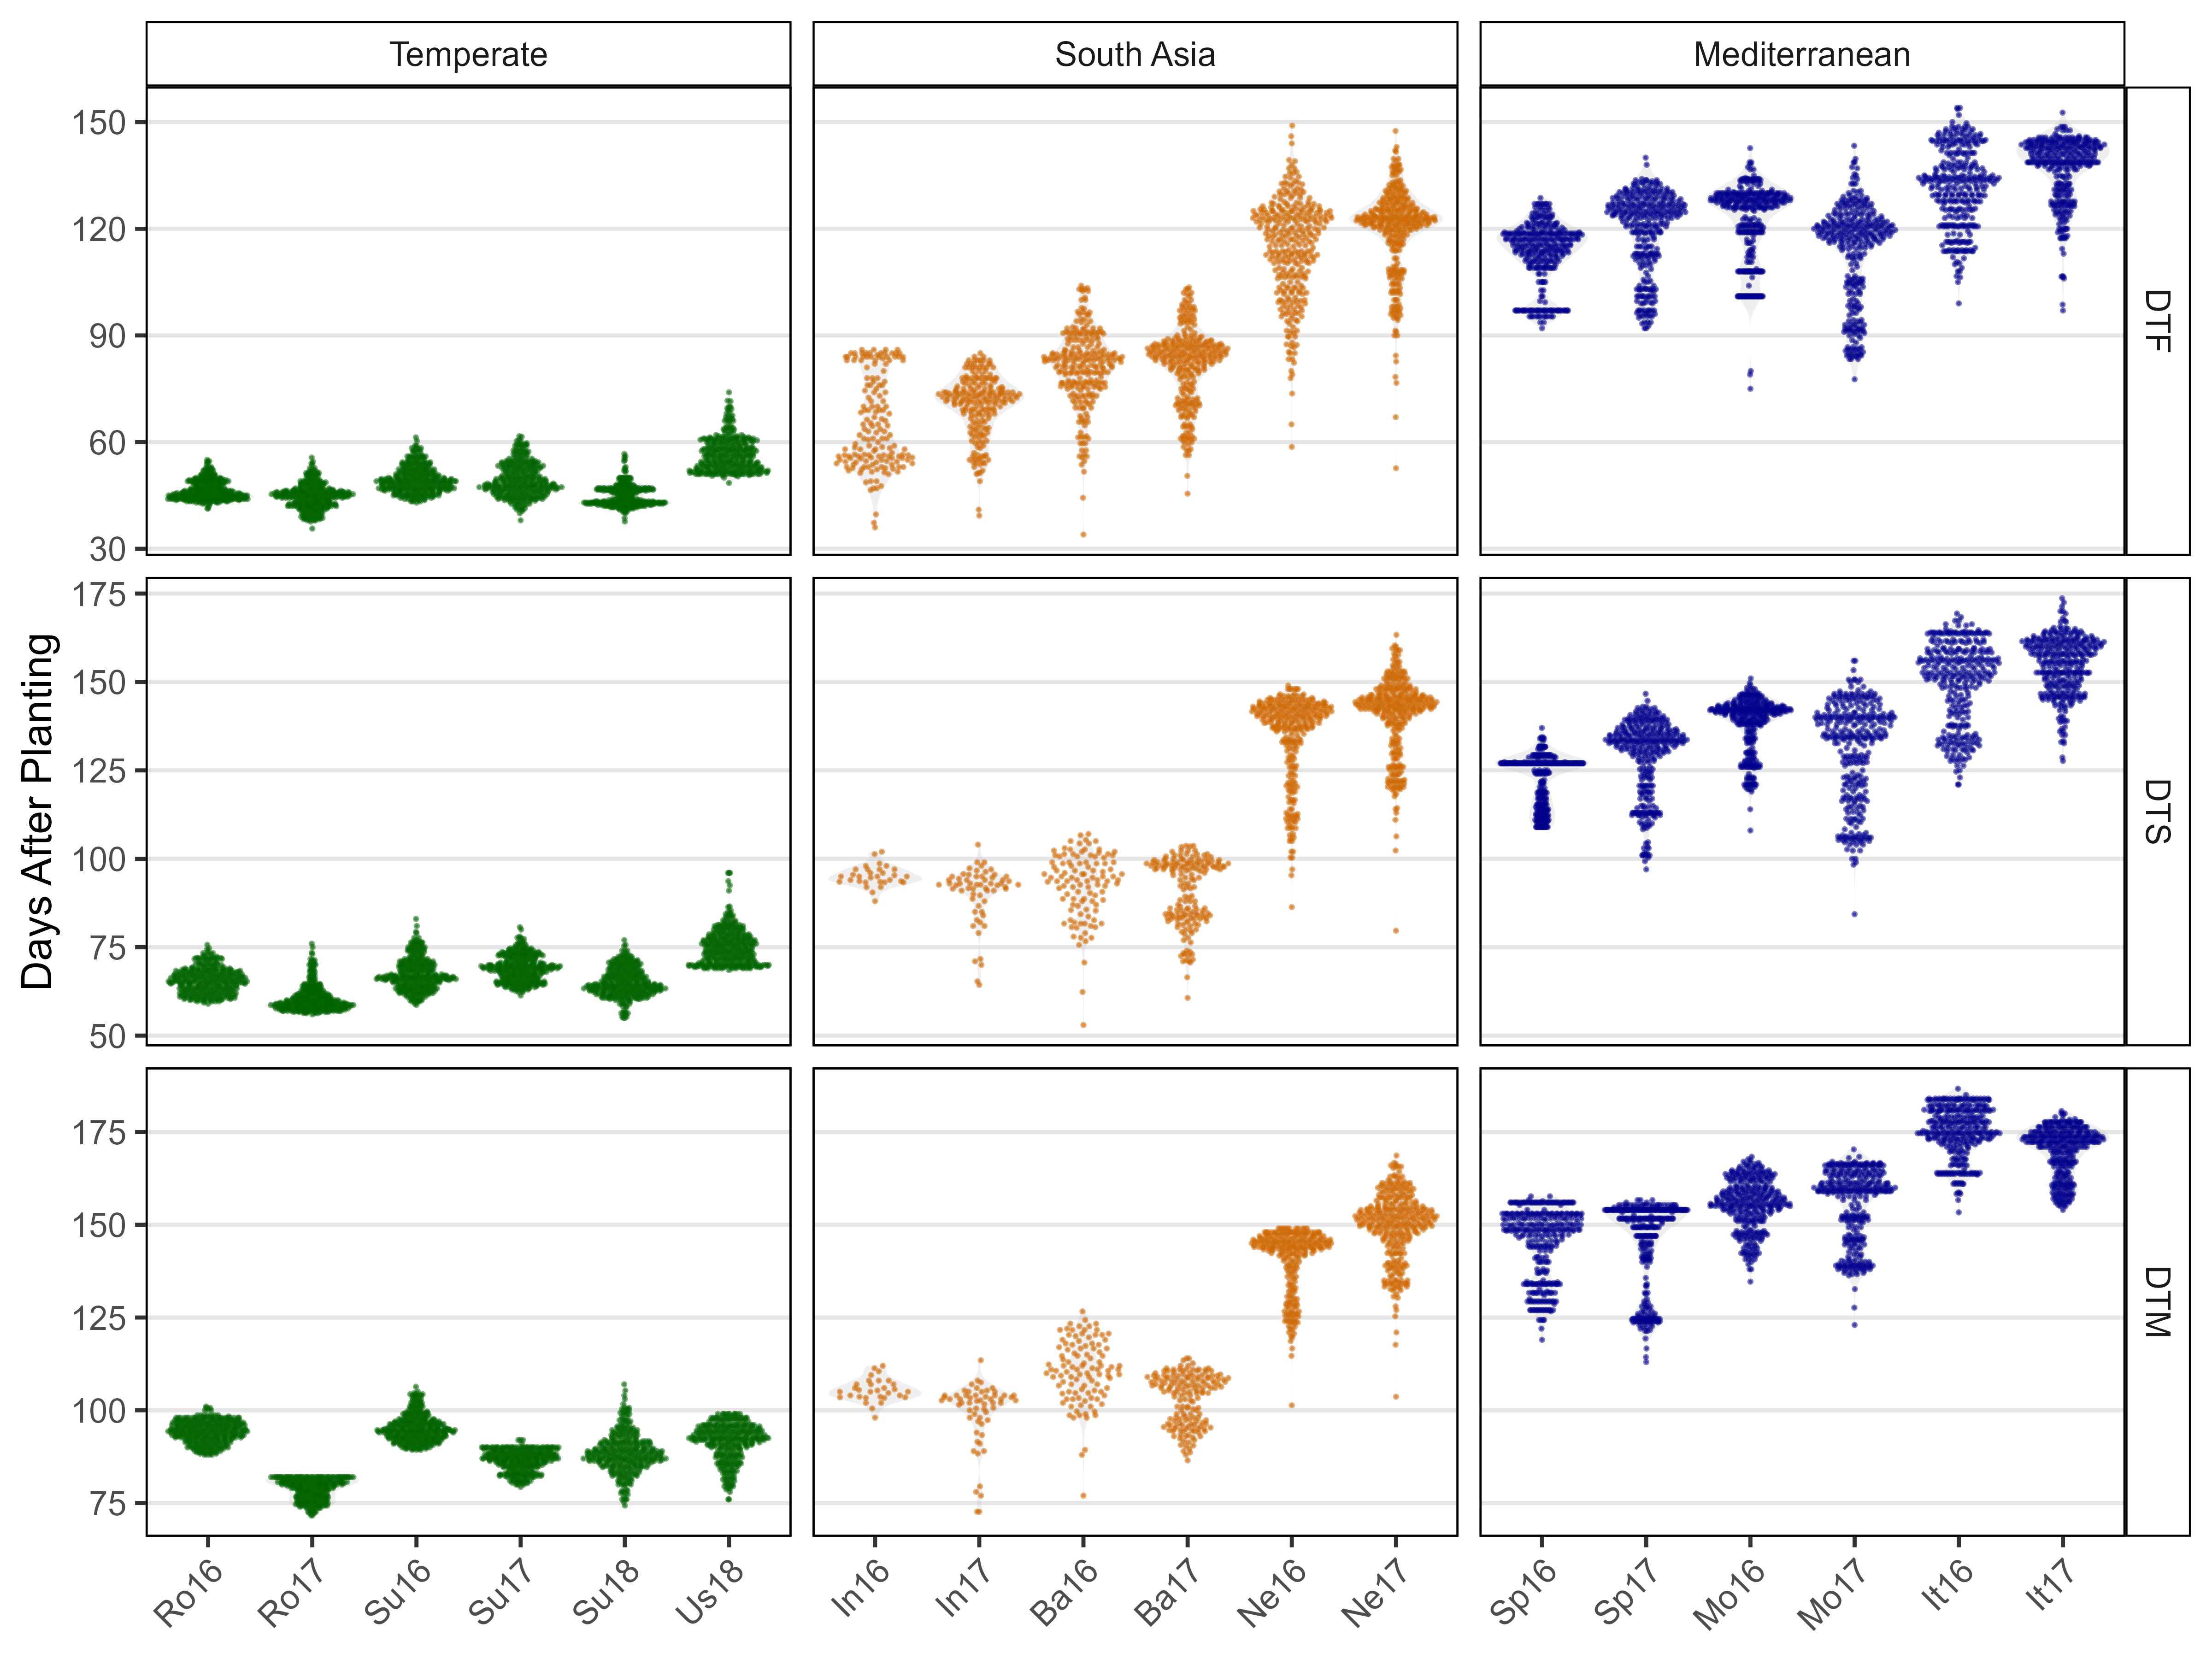
\includegraphics{Additional/Additional_Figure_02.png}

\begin{Shaded}
\begin{Highlighting}[]
\CommentTok{# Prep data}
\NormalTok{xx <-}\StringTok{ }\NormalTok{dd }\OperatorTok\StringTok{ }\KeywordTok{select}\NormalTok{(Entry, Expt, ExptShort, DTF, DTS, DTM) }\OperatorTok
\StringTok{  }\KeywordTok{left_join}\NormalTok{(}\KeywordTok{select}\NormalTok{(ff, Expt, MacroEnv), }\DataTypeTok{by =} \StringTok{"Expt"}\NormalTok{) }\OperatorTok
\StringTok{  }\KeywordTok{gather}\NormalTok{(Trait, Value, DTF, DTS, DTM) }\OperatorTok\StringTok{ }
\StringTok{  }\KeywordTok{mutate}\NormalTok{(}\DataTypeTok{Trait =} \KeywordTok{factor}\NormalTok{(Trait, }\DataTypeTok{levels =} \KeywordTok{c}\NormalTok{(}\StringTok{"DTF"}\NormalTok{, }\StringTok{"DTS"}\NormalTok{, }\StringTok{"DTM"}\NormalTok{)) )}
\CommentTok{# Plot}
\NormalTok{mp <-}\StringTok{ }\KeywordTok{ggplot}\NormalTok{(xx, }\KeywordTok{aes}\NormalTok{(}\DataTypeTok{x =}\NormalTok{ Expt, }\DataTypeTok{y =}\NormalTok{ Value)) }\OperatorTok{+}
\StringTok{  }\KeywordTok{geom_violin}\NormalTok{(}\DataTypeTok{fill =} \StringTok{"grey"}\NormalTok{, }\DataTypeTok{alpha =} \FloatTok{0.25}\NormalTok{, }\DataTypeTok{color =} \OtherTok{NA}\NormalTok{) }\OperatorTok{+}\StringTok{ }
\StringTok{  }\KeywordTok{geom_quasirandom}\NormalTok{(}\DataTypeTok{size =} \FloatTok{0.1}\NormalTok{, }\DataTypeTok{alpha =} \FloatTok{0.5}\NormalTok{, }\KeywordTok{aes}\NormalTok{(}\DataTypeTok{color =}\NormalTok{ MacroEnv)) }\OperatorTok{+}
\StringTok{  }\KeywordTok{facet_grid}\NormalTok{(Trait }\OperatorTok{~}\StringTok{ }\NormalTok{MacroEnv, }\DataTypeTok{scales =} \StringTok{"free"}\NormalTok{) }\OperatorTok{+}\StringTok{ }
\StringTok{  }\KeywordTok{scale_color_manual}\NormalTok{(}\DataTypeTok{values =} \KeywordTok{c}\NormalTok{(}\StringTok{"darkgreen"}\NormalTok{, }\StringTok{"darkorange3"}\NormalTok{, }\StringTok{"darkblue"}\NormalTok{)) }\OperatorTok{+}
\StringTok{  }\NormalTok{theme_AGL }\OperatorTok{+}
\StringTok{  }\KeywordTok{theme}\NormalTok{(}\DataTypeTok{legend.position =} \StringTok{"none"}\NormalTok{,}
        \DataTypeTok{panel.grid.major.x =} \KeywordTok{element_blank}\NormalTok{(),}
        \DataTypeTok{axis.text.x =} \KeywordTok{element_text}\NormalTok{(}\DataTypeTok{angle =} \DecValTok{90}\NormalTok{, }\DataTypeTok{vjust =} \FloatTok{0.5}\NormalTok{, }\DataTypeTok{hjust =} \DecValTok{1}\NormalTok{)) }\OperatorTok{+}
\StringTok{  }\KeywordTok{labs}\NormalTok{(}\DataTypeTok{x =} \OtherTok{NULL}\NormalTok{, }\DataTypeTok{y =} \StringTok{"Days After Planting"}\NormalTok{)}
\KeywordTok{ggsave}\NormalTok{(}\StringTok{"Additional/Additional_Figure_02.png"}\NormalTok{, mp, }\DataTypeTok{width =} \DecValTok{8}\NormalTok{, }\DataTypeTok{height =} \DecValTok{6}\NormalTok{, }\DataTypeTok{dpi =} \DecValTok{600}\NormalTok{)}
\end{Highlighting}
\end{Shaded}

\hypertarget{additional-figure-3-macroenv-phenology}{%
\subsection{Additional Figure 3 MacroEnv
Phenology}\label{additional-figure-3-macroenv-phenology}}

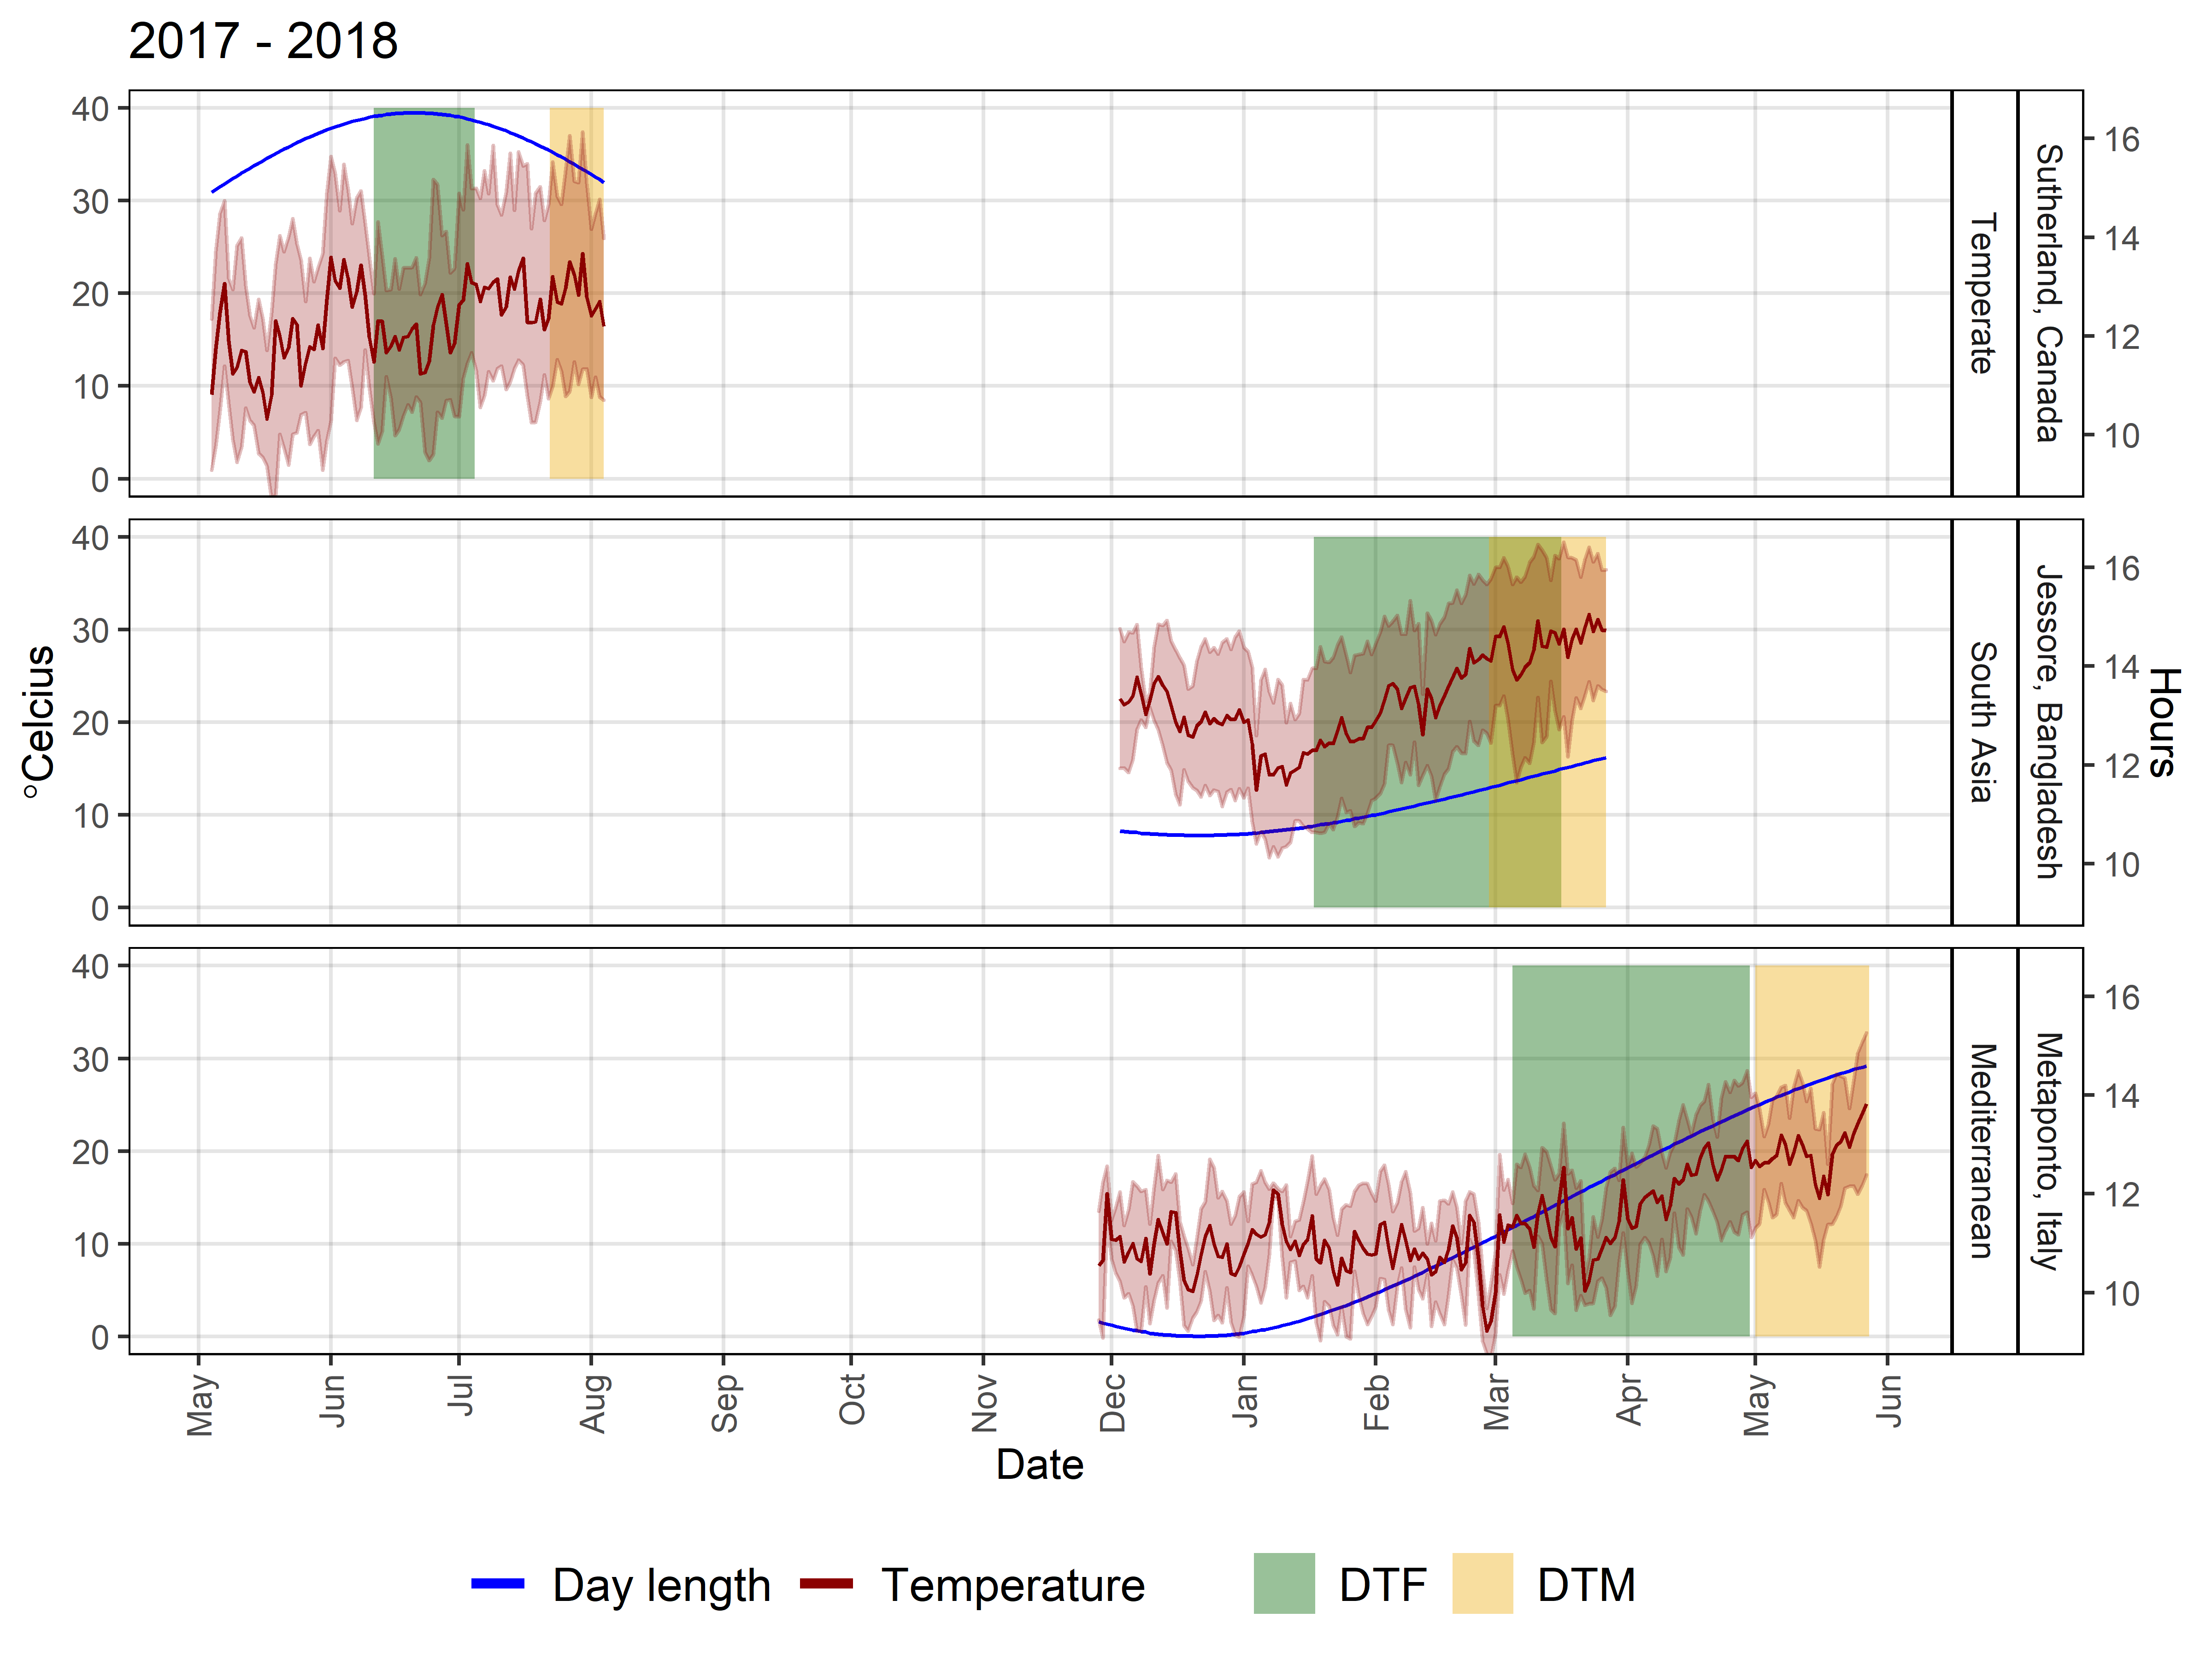
\includegraphics{Additional/Additional_Figure_03.png}

\begin{Shaded}
\begin{Highlighting}[]
\CommentTok{# Prep data}
\NormalTok{xx <-}\StringTok{ }\NormalTok{ee }\OperatorTok\StringTok{ }\KeywordTok{filter}\NormalTok{(ExptShort }\OperatorTok\StringTok{ }\KeywordTok{c}\NormalTok{(}\StringTok{"Su17"}\NormalTok{, }\StringTok{"Ba17"}\NormalTok{, }\StringTok{"It17"}\NormalTok{)) }
\NormalTok{yy <-}\StringTok{ }\NormalTok{ff }\OperatorTok\StringTok{ }\KeywordTok{filter}\NormalTok{(Expt }\OperatorTok\StringTok{ }\KeywordTok{unique}\NormalTok{(xx}\OperatorTok{$}\NormalTok{Expt)) }\OperatorTok\StringTok{ }
\StringTok{  }\KeywordTok{mutate}\NormalTok{(}\DataTypeTok{DTF_min =}\NormalTok{ Start }\OperatorTok{+}\StringTok{ }\NormalTok{DTF_min, }\DataTypeTok{DTF_max =}\NormalTok{ Start }\OperatorTok{+}\StringTok{ }\NormalTok{DTF_max,}
         \DataTypeTok{DTM_min =}\NormalTok{ Start }\OperatorTok{+}\StringTok{ }\NormalTok{DTM_min, }\DataTypeTok{DTM_max =}\NormalTok{ Start }\OperatorTok{+}\StringTok{ }\NormalTok{DTM_max)}
\NormalTok{y1 <-}\StringTok{ }\KeywordTok{select}\NormalTok{(yy, Expt, Location, Year, MacroEnv, }\DataTypeTok{min =}\NormalTok{ DTF_min, }\DataTypeTok{max =}\NormalTok{ DTF_max) }\OperatorTok\StringTok{ }
\StringTok{  }\KeywordTok{mutate}\NormalTok{(}\DataTypeTok{Trait =} \StringTok{"DTF"}\NormalTok{)}
\NormalTok{y2 <-}\StringTok{ }\KeywordTok{select}\NormalTok{(yy, Expt, Location, Year, MacroEnv, }\DataTypeTok{min =}\NormalTok{ DTM_min, }\DataTypeTok{max =}\NormalTok{ DTM_max) }\OperatorTok\StringTok{ }
\StringTok{  }\KeywordTok{mutate}\NormalTok{(}\DataTypeTok{Trait =} \StringTok{"DTM"}\NormalTok{)}
\NormalTok{yy <-}\StringTok{ }\KeywordTok{bind_rows}\NormalTok{(y1, y2)}
\CommentTok{# Plot}
\NormalTok{mp <-}\StringTok{ }\KeywordTok{ggplot}\NormalTok{(xx) }\OperatorTok{+}
\StringTok{  }\KeywordTok{geom_rect}\NormalTok{(}\DataTypeTok{data =}\NormalTok{ yy, }\KeywordTok{aes}\NormalTok{(}\DataTypeTok{xmin =}\NormalTok{ min, }\DataTypeTok{xmax =}\NormalTok{ max, }\DataTypeTok{fill =}\NormalTok{ Trait), }
            \DataTypeTok{ymin =} \DecValTok{0}\NormalTok{, }\DataTypeTok{ymax =} \DecValTok{40}\NormalTok{, }\DataTypeTok{alpha =} \FloatTok{0.4}\NormalTok{) }\OperatorTok{+}
\StringTok{  }\KeywordTok{geom_line}\NormalTok{(}\KeywordTok{aes}\NormalTok{(}\DataTypeTok{x =}\NormalTok{ Date, }\DataTypeTok{y =}\NormalTok{ DayLength_rescaled, }\DataTypeTok{color =} \StringTok{"Blue"}\NormalTok{)) }\OperatorTok{+}
\StringTok{  }\KeywordTok{geom_line}\NormalTok{(}\KeywordTok{aes}\NormalTok{(}\DataTypeTok{x =}\NormalTok{ Date, }\DataTypeTok{y =}\NormalTok{ Temp_mean, }\DataTypeTok{color =} \StringTok{"darkred"}\NormalTok{) ) }\OperatorTok{+}
\StringTok{  }\KeywordTok{geom_ribbon}\NormalTok{(}\KeywordTok{aes}\NormalTok{(}\DataTypeTok{x =}\NormalTok{ Date, }\DataTypeTok{ymin =}\NormalTok{ Temp_min, }\DataTypeTok{ymax =}\NormalTok{ Temp_max),}
              \DataTypeTok{fill =} \KeywordTok{alpha}\NormalTok{(}\StringTok{"darkred"}\NormalTok{, }\FloatTok{0.25}\NormalTok{), }\DataTypeTok{color =} \KeywordTok{alpha}\NormalTok{(}\StringTok{"darkred"}\NormalTok{, }\FloatTok{0.25}\NormalTok{)) }\OperatorTok{+}
\StringTok{  }\KeywordTok{facet_grid}\NormalTok{(Location }\OperatorTok{+}\NormalTok{MacroEnv  }\OperatorTok{~}\StringTok{ }\NormalTok{., }\DataTypeTok{scales =} \StringTok{"free_x"}\NormalTok{, }\DataTypeTok{space =} \StringTok{"free_x"}\NormalTok{) }\OperatorTok{+}
\StringTok{  }\KeywordTok{scale_color_manual}\NormalTok{(}\DataTypeTok{name =} \OtherTok{NULL}\NormalTok{, }\DataTypeTok{values =} \KeywordTok{c}\NormalTok{(}\StringTok{"Blue"}\NormalTok{, }\StringTok{"darkred"}\NormalTok{), }
                    \DataTypeTok{labels =} \KeywordTok{c}\NormalTok{(}\StringTok{"Day length"}\NormalTok{, }\StringTok{"Temperature"}\NormalTok{) ) }\OperatorTok{+}
\StringTok{  }\KeywordTok{scale_fill_manual}\NormalTok{(}\DataTypeTok{name =} \OtherTok{NULL}\NormalTok{, }\DataTypeTok{values =} \KeywordTok{c}\NormalTok{(}\StringTok{"darkgreen"}\NormalTok{, }\StringTok{"darkgoldenrod2"}\NormalTok{)) }\OperatorTok{+}
\StringTok{  }\KeywordTok{coord_cartesian}\NormalTok{(}\DataTypeTok{ylim =} \KeywordTok{c}\NormalTok{(}\DecValTok{0}\NormalTok{,}\DecValTok{40}\NormalTok{)) }\OperatorTok{+}
\StringTok{  }\NormalTok{theme_AGL }\OperatorTok{+}
\StringTok{  }\KeywordTok{theme}\NormalTok{(}\DataTypeTok{legend.position =} \StringTok{"bottom"}\NormalTok{, }
        \DataTypeTok{legend.text =} \KeywordTok{element_text}\NormalTok{(}\DataTypeTok{size =} \DecValTok{12}\NormalTok{),}
        \DataTypeTok{axis.text.x =} \KeywordTok{element_text}\NormalTok{(}\DataTypeTok{angle =} \DecValTok{90}\NormalTok{, }\DataTypeTok{hjust =} \DecValTok{1}\NormalTok{, }\DataTypeTok{vjust =} \FloatTok{0.5}\NormalTok{)) }\OperatorTok{+}
\StringTok{  }\KeywordTok{scale_x_date}\NormalTok{(}\DataTypeTok{breaks =} \StringTok{"1 month"}\NormalTok{, }\DataTypeTok{labels =} \KeywordTok{date_format}\NormalTok{(}\StringTok{"%B"}\NormalTok{)) }\OperatorTok{+}
\StringTok{  }\KeywordTok{scale_y_continuous}\NormalTok{(}\DataTypeTok{sec.axis =} \KeywordTok{sec_axis}\NormalTok{(}\OperatorTok{~}\StringTok{ }\NormalTok{(}\FloatTok{16.62} \OperatorTok{-}\StringTok{ }\FloatTok{9.11}\NormalTok{) }\OperatorTok{*}\StringTok{ }\NormalTok{. }\OperatorTok{/}\StringTok{ }\NormalTok{(}\DecValTok{40} \OperatorTok{-}\StringTok{ }\DecValTok{0}\NormalTok{) }\OperatorTok{+}\StringTok{ }\FloatTok{9.11}\NormalTok{, }
                     \DataTypeTok{breaks =} \KeywordTok{c}\NormalTok{(}\DecValTok{10}\NormalTok{, }\DecValTok{12}\NormalTok{, }\DecValTok{14}\NormalTok{, }\DecValTok{16}\NormalTok{), }\DataTypeTok{name =} \StringTok{"Hours"}\NormalTok{)) }\OperatorTok{+}
\StringTok{  }\KeywordTok{labs}\NormalTok{(}\DataTypeTok{title =} \StringTok{"2017 - 2018"}\NormalTok{, }\DataTypeTok{y =} \KeywordTok{expression}\NormalTok{(}\KeywordTok{paste}\NormalTok{(degree, }\StringTok{"Celcius"}\NormalTok{), }\DataTypeTok{x =} \OtherTok{NULL}\NormalTok{)) }\OperatorTok{+}
\StringTok{  }\KeywordTok{guides}\NormalTok{(}\DataTypeTok{colour =} \KeywordTok{guide_legend}\NormalTok{(}\DataTypeTok{order =} \DecValTok{1}\NormalTok{, }\DataTypeTok{override.aes =} \KeywordTok{list}\NormalTok{(}\DataTypeTok{size =} \FloatTok{1.25}\NormalTok{)), }
         \DataTypeTok{fill   =} \KeywordTok{guide_legend}\NormalTok{(}\DataTypeTok{order =} \DecValTok{2}\NormalTok{))}
\KeywordTok{ggsave}\NormalTok{(}\StringTok{"Additional/Additional_Figure_03.png"}\NormalTok{, mp, }\DataTypeTok{width =} \DecValTok{8}\NormalTok{, }\DataTypeTok{height =} \DecValTok{6}\NormalTok{, }\DataTypeTok{dpi =} \DecValTok{600}\NormalTok{)}
\end{Highlighting}
\end{Shaded}

\hypertarget{additional-figure-4-ggridges}{%
\subsection{Additional Figure 4
ggridges}\label{additional-figure-4-ggridges}}

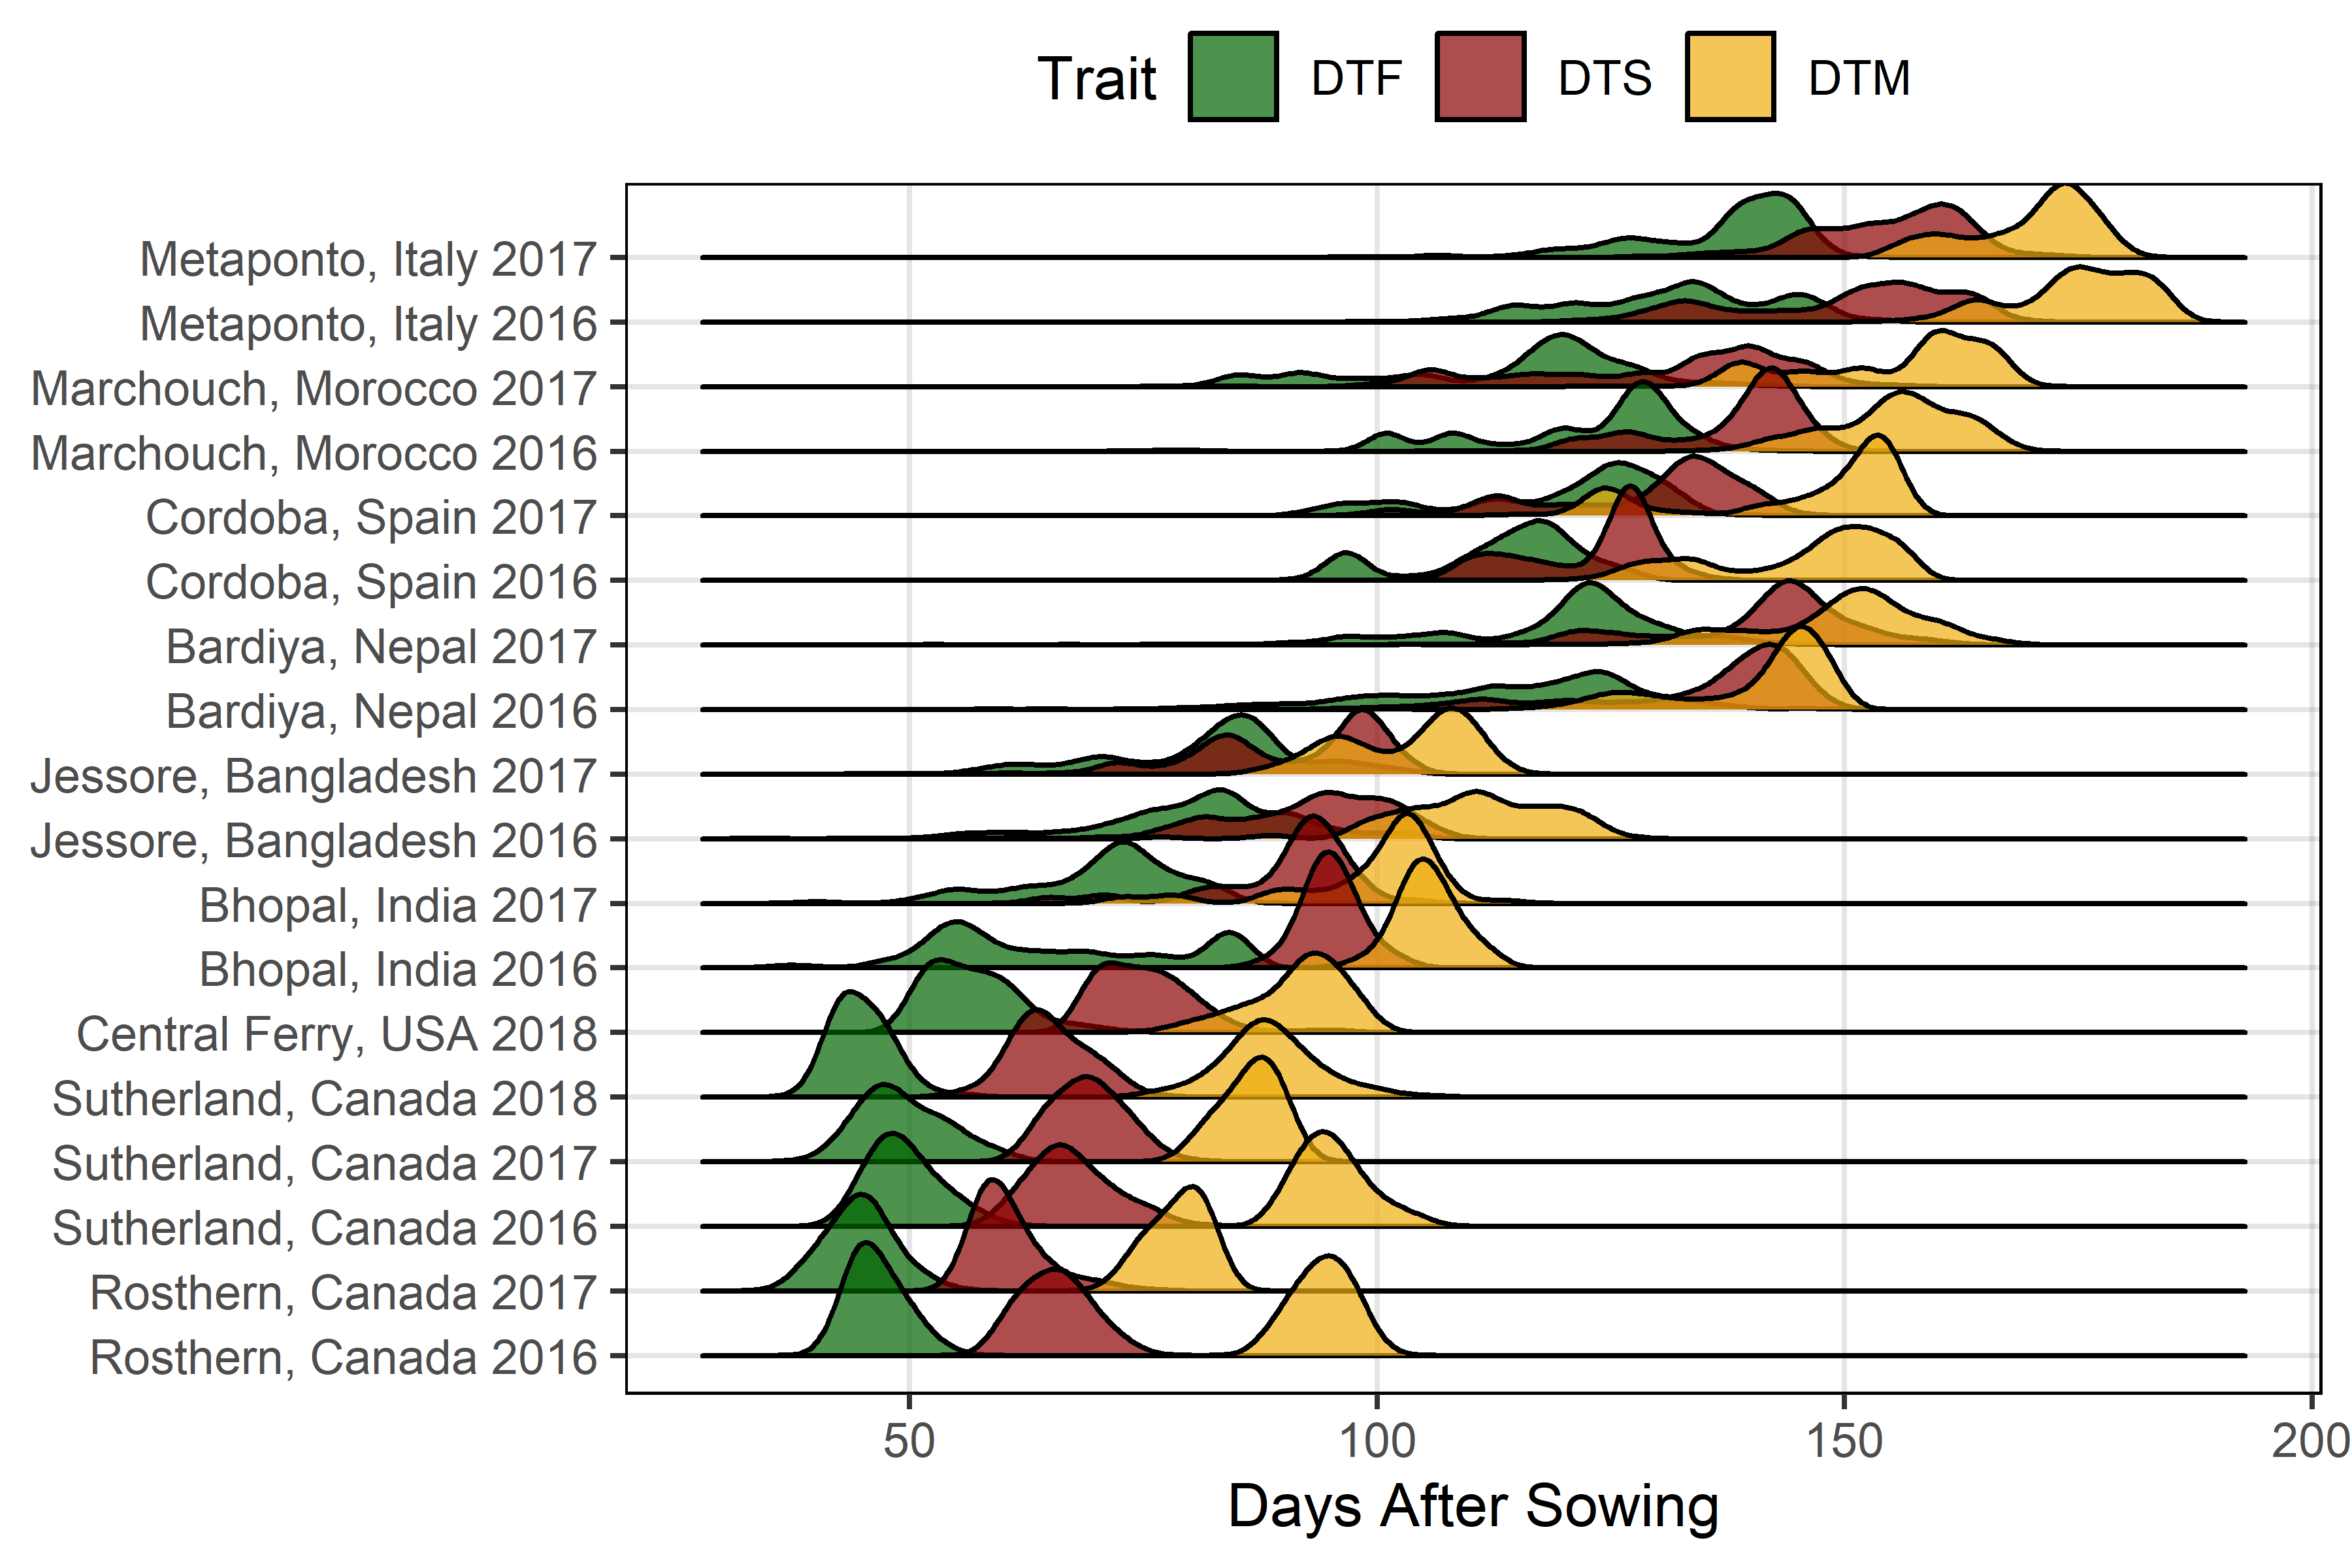
\includegraphics{Additional/Additional_Figure_04.png}

\begin{Shaded}
\begin{Highlighting}[]
\CommentTok{# Prep data}
\NormalTok{xx <-}\StringTok{ }\NormalTok{dd }\OperatorTok\StringTok{ }\KeywordTok{select}\NormalTok{(Expt, DTF, DTS, DTM) }\OperatorTok\StringTok{ }
\StringTok{  }\KeywordTok{gather}\NormalTok{(Trait, Value, DTF, DTS, DTM) }\OperatorTok
\StringTok{  }\KeywordTok{mutate}\NormalTok{(}\DataTypeTok{Trait =} \KeywordTok{factor}\NormalTok{(Trait, }\DataTypeTok{levels =} \KeywordTok{c}\NormalTok{(}\StringTok{"DTF"}\NormalTok{, }\StringTok{"DTS"}\NormalTok{, }\StringTok{"DTM"}\NormalTok{)))}
\CommentTok{# Plot}
\NormalTok{mp <-}\StringTok{ }\KeywordTok{ggplot}\NormalTok{(xx, }\KeywordTok{aes}\NormalTok{(}\DataTypeTok{x =}\NormalTok{ Value, }\DataTypeTok{y =}\NormalTok{ Expt, }\DataTypeTok{fill =}\NormalTok{ Trait)) }\OperatorTok{+}\StringTok{ }
\StringTok{  }\NormalTok{ggridges}\OperatorTok{::}\KeywordTok{geom_density_ridges}\NormalTok{(}\DataTypeTok{alpha =} \FloatTok{0.7}\NormalTok{) }\OperatorTok{+}
\StringTok{  }\KeywordTok{scale_fill_manual}\NormalTok{(}\DataTypeTok{values =} \KeywordTok{c}\NormalTok{(}\StringTok{"darkgreen"}\NormalTok{, }\StringTok{"darkred"}\NormalTok{, }\StringTok{"darkgoldenrod2"}\NormalTok{)) }\OperatorTok{+}
\StringTok{  }\NormalTok{theme_AGL }\OperatorTok{+}
\StringTok{  }\KeywordTok{theme}\NormalTok{(}\DataTypeTok{legend.position =} \StringTok{"top"}\NormalTok{, }\DataTypeTok{legend.margin =} \KeywordTok{unit}\NormalTok{(}\KeywordTok{c}\NormalTok{(}\DecValTok{0}\NormalTok{,}\DecValTok{0}\NormalTok{,}\DecValTok{0}\NormalTok{,}\DecValTok{0}\NormalTok{), }\StringTok{"cm"}\NormalTok{)) }\OperatorTok{+}
\StringTok{  }\KeywordTok{labs}\NormalTok{(}\DataTypeTok{y =} \OtherTok{NULL}\NormalTok{, }\DataTypeTok{x =} \StringTok{"Days After Sowing"}\NormalTok{)}
\KeywordTok{ggsave}\NormalTok{(}\StringTok{"Additional/Additional_Figure_04.png"}\NormalTok{, mp, }\DataTypeTok{width =} \DecValTok{6}\NormalTok{, }\DataTypeTok{height =} \DecValTok{4}\NormalTok{, }\DataTypeTok{dpi =} \DecValTok{600}\NormalTok{)}
\end{Highlighting}
\end{Shaded}

\hypertarget{supplemental-figure-2-missing-data}{%
\subsection{Supplemental Figure 2 Missing
Data}\label{supplemental-figure-2-missing-data}}

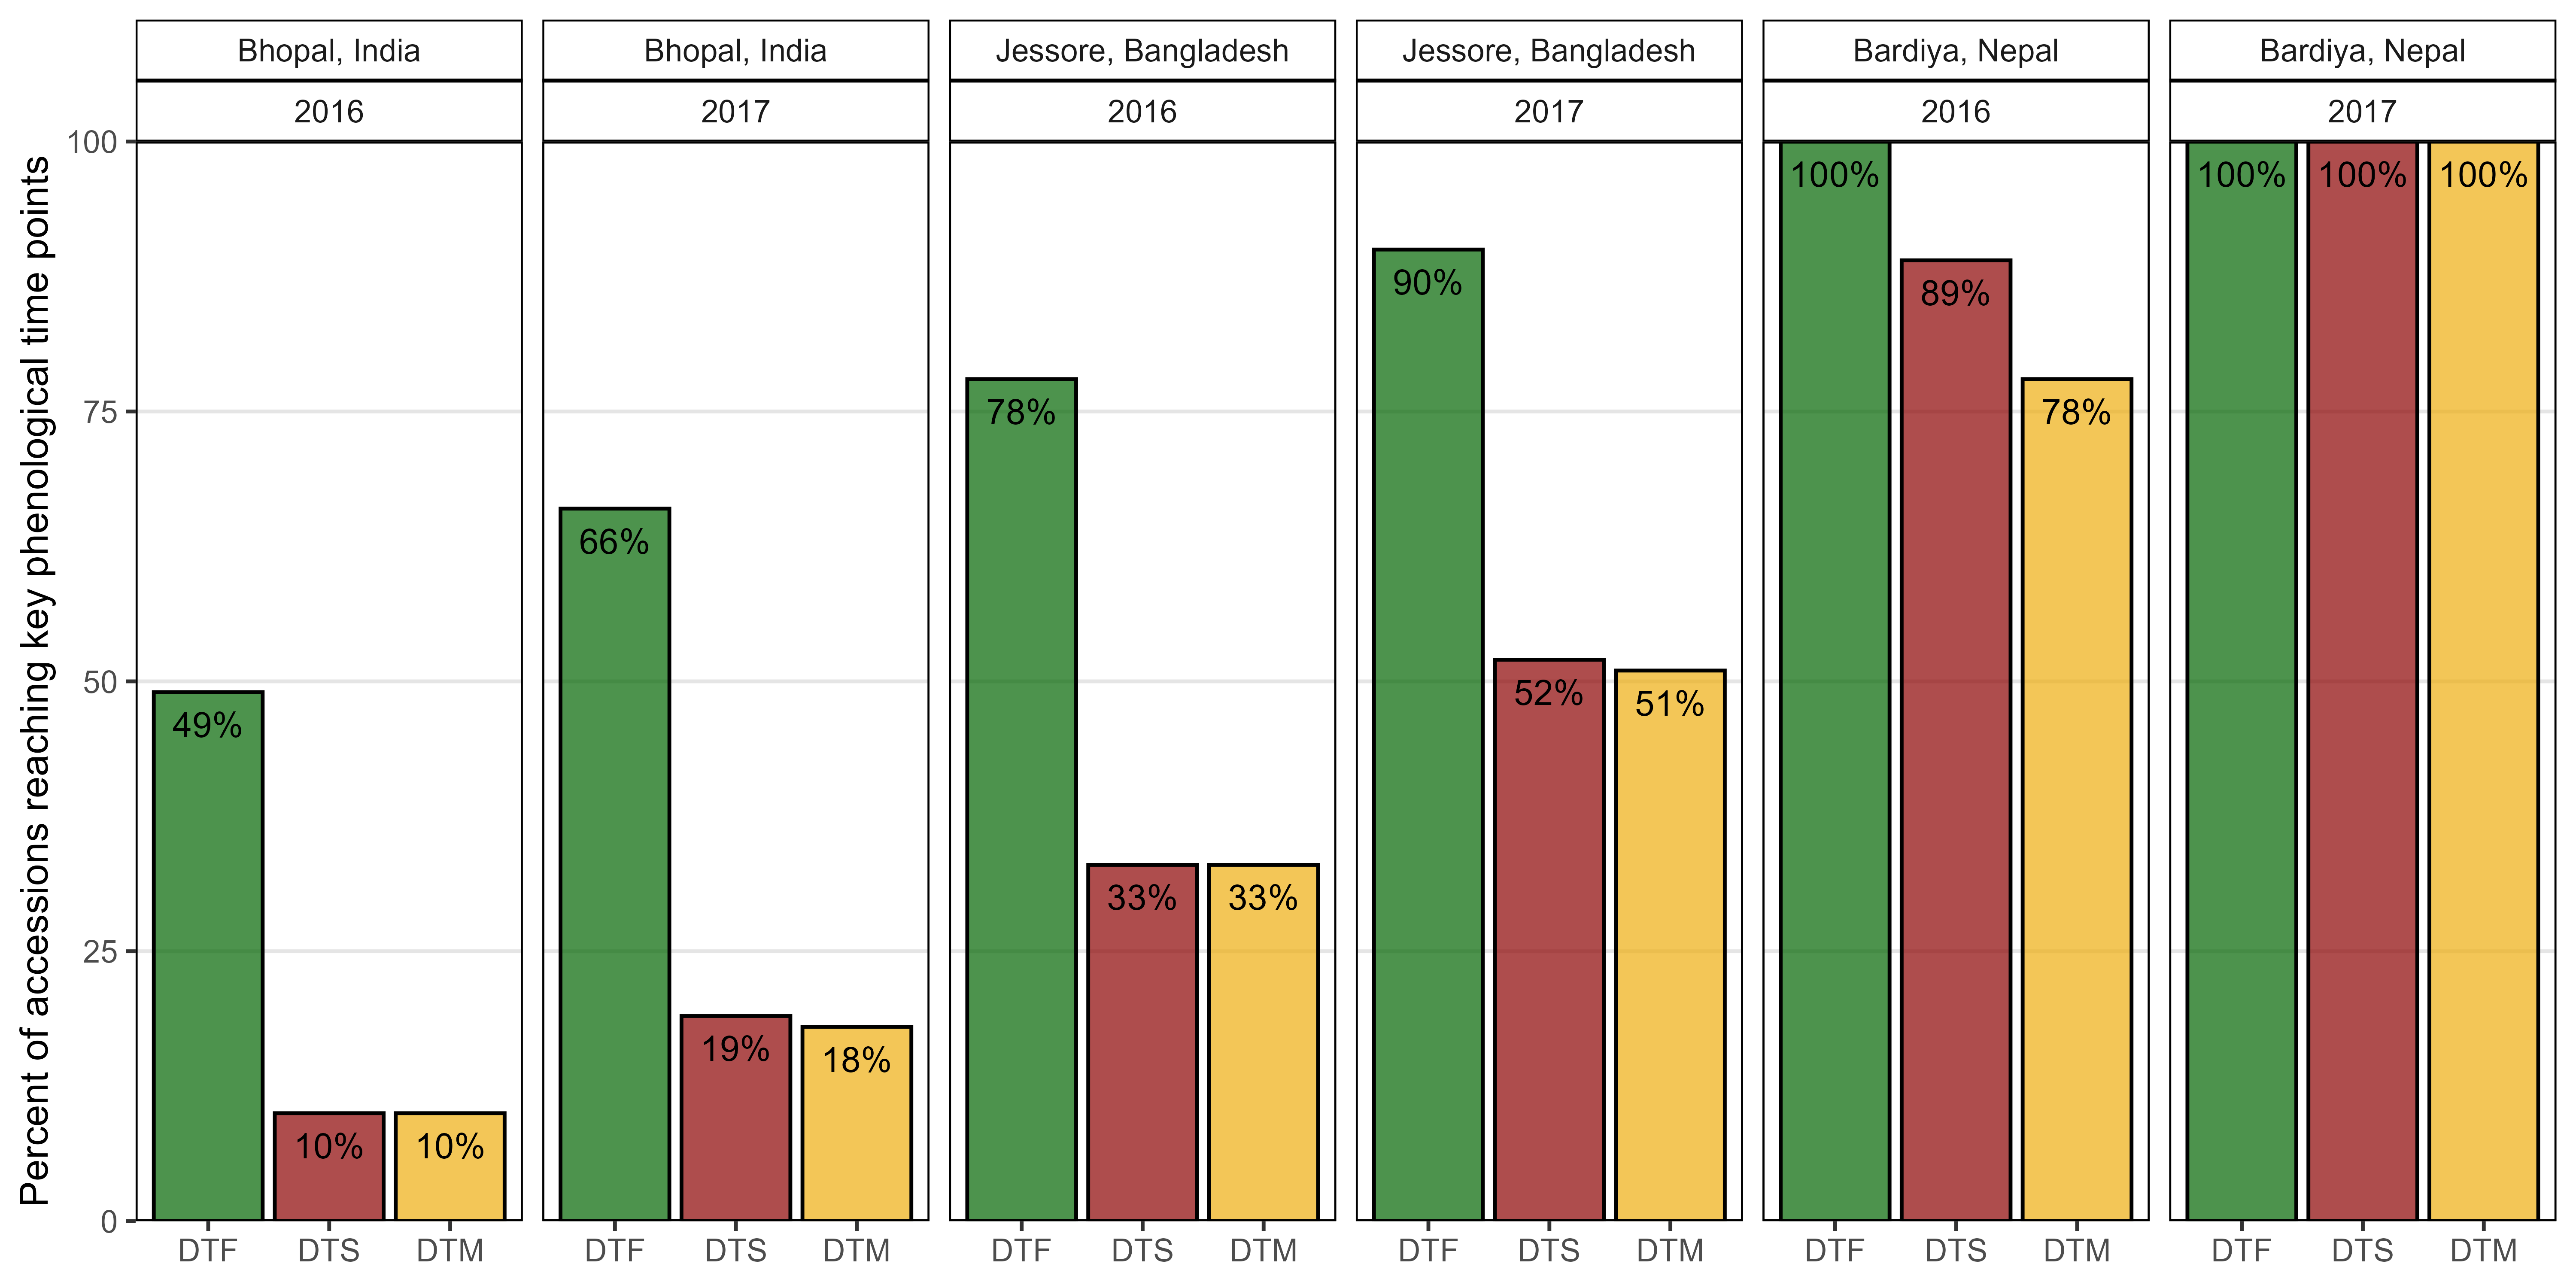
\includegraphics{Supplemental_Figure_02.png}

\begin{Shaded}
\begin{Highlighting}[]
\CommentTok{# Prep data}
\NormalTok{xx <-}\StringTok{ }\NormalTok{dd }\OperatorTok\StringTok{ }
\StringTok{  }\KeywordTok{filter}\NormalTok{(Location }\OperatorTok\StringTok{ }\KeywordTok{c}\NormalTok{(}\StringTok{"Bhopal, India"}\NormalTok{, }\StringTok{"Jessore, Bangladesh"}\NormalTok{, }\StringTok{"Bardiya, Nepal"}\NormalTok{)) }\OperatorTok
\StringTok{  }\KeywordTok{mutate}\NormalTok{(}\DataTypeTok{DTF =} \KeywordTok{ifelse}\NormalTok{(}\KeywordTok{is.na}\NormalTok{(DTF), }\DecValTok{0}\NormalTok{, }\DecValTok{1}\NormalTok{),}
         \DataTypeTok{DTS =} \KeywordTok{ifelse}\NormalTok{(}\KeywordTok{is.na}\NormalTok{(DTS), }\DecValTok{0}\NormalTok{, }\DecValTok{1}\NormalTok{),}
         \DataTypeTok{DTM =} \KeywordTok{ifelse}\NormalTok{(}\KeywordTok{is.na}\NormalTok{(DTM), }\DecValTok{0}\NormalTok{, }\DecValTok{1}\NormalTok{) ) }\OperatorTok\StringTok{ }
\StringTok{  }\KeywordTok{group_by}\NormalTok{(Expt, Location, Year) }\OperatorTok\StringTok{ }
\StringTok{  }\KeywordTok{summarise_at}\NormalTok{(}\KeywordTok{vars}\NormalTok{(DTF, DTS, DTM), }\KeywordTok{funs}\NormalTok{(sum), }\DataTypeTok{na.rm =}\NormalTok{ T) }\OperatorTok
\StringTok{  }\KeywordTok{ungroup}\NormalTok{() }\OperatorTok\StringTok{ }
\StringTok{  }\KeywordTok{gather}\NormalTok{(Trait, Flowered, DTF, DTS, DTM) }\OperatorTok
\StringTok{  }\KeywordTok{mutate}\NormalTok{(}\DataTypeTok{Total =} \KeywordTok{ifelse}\NormalTok{(Expt }\OperatorTok{==}\StringTok{ "Bardiya, Nepal 2016"}\NormalTok{, }\DecValTok{323}\NormalTok{, }\DecValTok{324}\NormalTok{),}
         \CommentTok{# One accession was not planted in Bardiya, Nepal 2016}
         \DataTypeTok{DidNotFlower =}\NormalTok{ Total }\OperatorTok{-}\StringTok{ }\NormalTok{Flowered,}
         \DataTypeTok{Percent =} \KeywordTok{round}\NormalTok{(}\DecValTok{100} \OperatorTok{*}\StringTok{ }\NormalTok{Flowered }\OperatorTok{/}\StringTok{ }\NormalTok{Total),}
         \DataTypeTok{Label =} \KeywordTok{paste0}\NormalTok{(Percent, }\StringTok{"%"}\NormalTok{),}
         \DataTypeTok{Trait =} \KeywordTok{factor}\NormalTok{(Trait, }\DataTypeTok{levels =} \KeywordTok{c}\NormalTok{(}\StringTok{"DTF"}\NormalTok{, }\StringTok{"DTS"}\NormalTok{, }\StringTok{"DTM"}\NormalTok{)))}
\CommentTok{# Plot}
\NormalTok{mp <-}\StringTok{ }\KeywordTok{ggplot}\NormalTok{(xx, }\KeywordTok{aes}\NormalTok{(}\DataTypeTok{x =}\NormalTok{ Trait, }\DataTypeTok{y =}\NormalTok{ Percent, }\DataTypeTok{fill =}\NormalTok{ Trait)) }\OperatorTok{+}\StringTok{ }
\StringTok{  }\KeywordTok{geom_bar}\NormalTok{(}\DataTypeTok{stat =} \StringTok{"identity"}\NormalTok{, }\DataTypeTok{color =} \StringTok{"black"}\NormalTok{, }\DataTypeTok{alpha =} \FloatTok{0.7}\NormalTok{) }\OperatorTok{+}\StringTok{ }
\StringTok{  }\KeywordTok{geom_text}\NormalTok{(}\KeywordTok{aes}\NormalTok{(}\DataTypeTok{label =}\NormalTok{ Label), }\DataTypeTok{nudge_y =} \DecValTok{-3}\NormalTok{, }\DataTypeTok{size =} \FloatTok{3.5}\NormalTok{) }\OperatorTok{+}\StringTok{ }
\StringTok{  }\KeywordTok{facet_grid}\NormalTok{(. }\OperatorTok{~}\StringTok{ }\NormalTok{Location }\OperatorTok{+}\StringTok{ }\NormalTok{Year) }\OperatorTok{+}\StringTok{ }
\StringTok{  }\KeywordTok{scale_fill_manual}\NormalTok{(}\DataTypeTok{values =} \KeywordTok{c}\NormalTok{(}\StringTok{"darkgreen"}\NormalTok{, }\StringTok{"darkred"}\NormalTok{, }\StringTok{"darkgoldenrod2"}\NormalTok{)) }\OperatorTok{+}\StringTok{ }
\StringTok{  }\KeywordTok{scale_y_continuous}\NormalTok{(}\DataTypeTok{limits =} \KeywordTok{c}\NormalTok{(}\DecValTok{0}\NormalTok{,}\DecValTok{100}\NormalTok{), }\DataTypeTok{expand =} \KeywordTok{c}\NormalTok{(}\DecValTok{0}\NormalTok{,}\DecValTok{0}\NormalTok{)) }\OperatorTok{+}
\StringTok{  }\NormalTok{theme_AGL }\OperatorTok{+}\StringTok{ }
\StringTok{  }\KeywordTok{theme}\NormalTok{(}\DataTypeTok{legend.position =} \StringTok{"none"}\NormalTok{,}
        \DataTypeTok{panel.grid.major.x =} \KeywordTok{element_blank}\NormalTok{() ) }\OperatorTok{+}\StringTok{ }
\StringTok{  }\KeywordTok{labs}\NormalTok{(}\DataTypeTok{x =} \OtherTok{NULL}\NormalTok{, }\DataTypeTok{y =} \StringTok{"Percent of accessions reaching key phenological time points"}\NormalTok{)}
\KeywordTok{ggsave}\NormalTok{(}\StringTok{"Supplemental_Figure_02.png"}\NormalTok{, }\DataTypeTok{width =} \DecValTok{10}\NormalTok{, }\DataTypeTok{height =} \DecValTok{5}\NormalTok{, }\DataTypeTok{dpi =} \DecValTok{600}\NormalTok{)}
\end{Highlighting}
\end{Shaded}

\hypertarget{supplemental-figure-3-correlation-plots}{%
\subsection{Supplemental Figure 3 Correlation
Plots}\label{supplemental-figure-3-correlation-plots}}

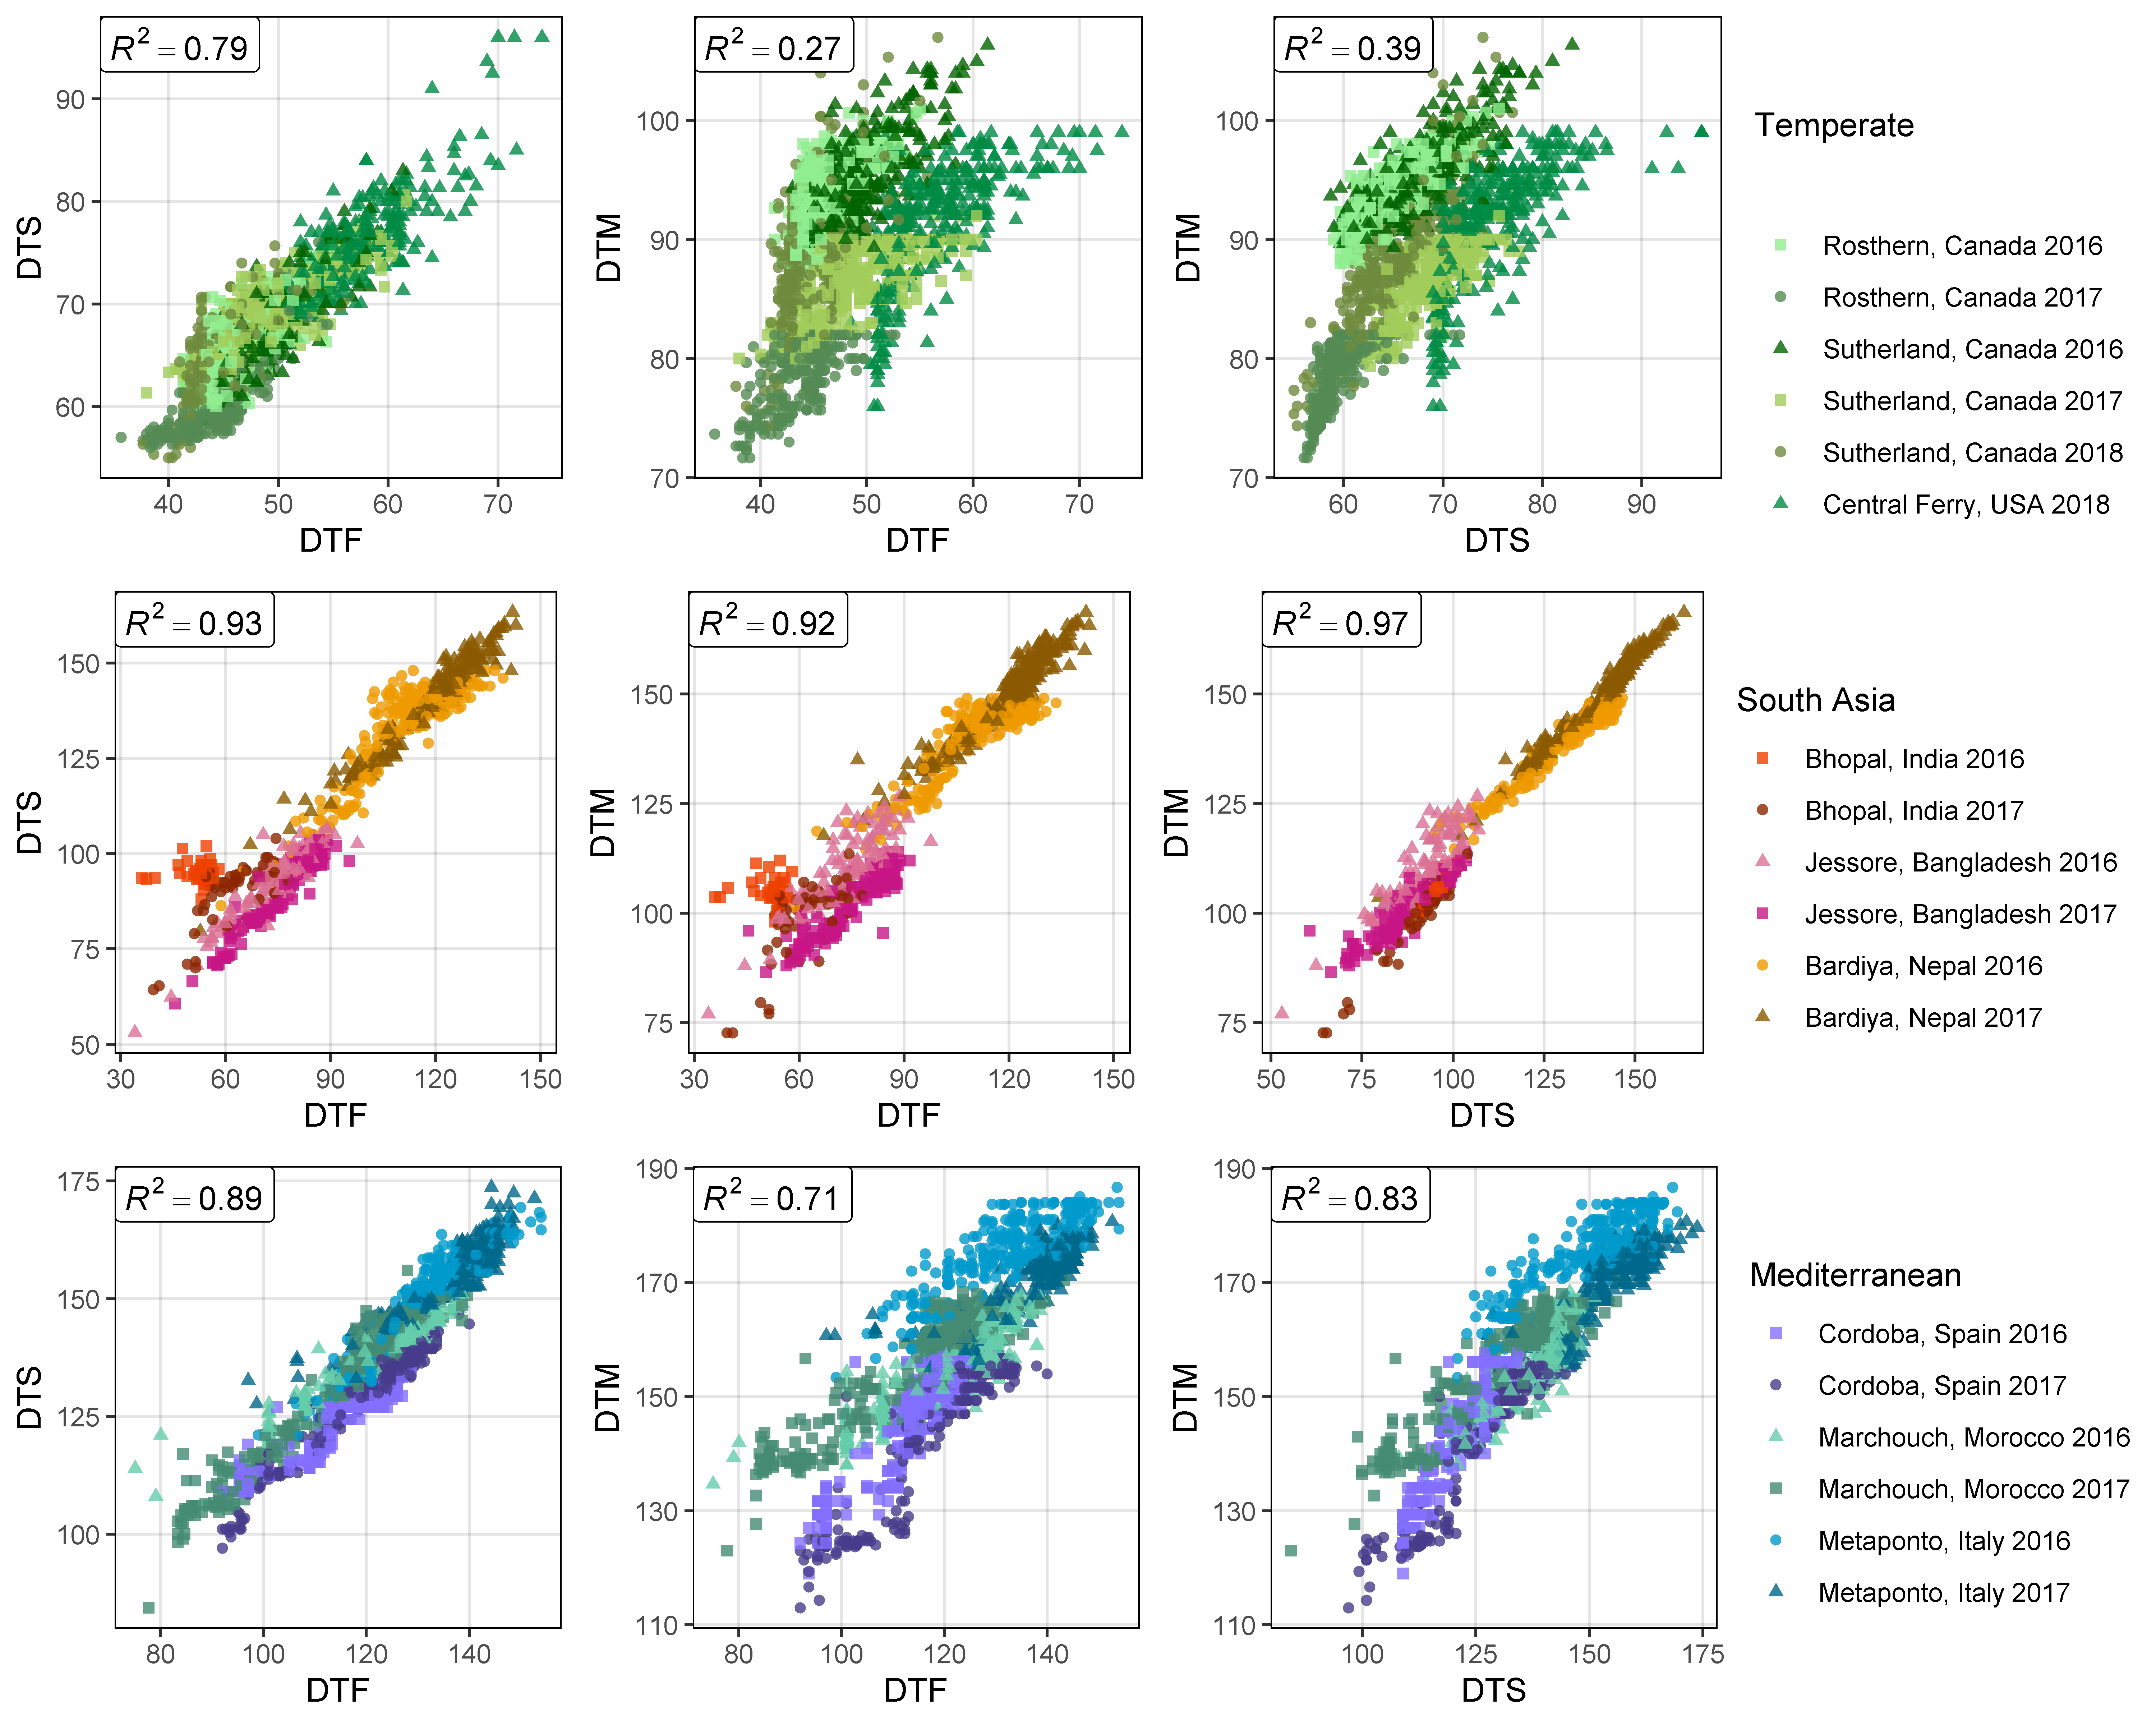
\includegraphics{Supplemental_Figure_03.png}

\begin{Shaded}
\begin{Highlighting}[]
\CommentTok{# Prep data}
\NormalTok{xx <-}\StringTok{ }\NormalTok{dd }\OperatorTok\StringTok{ }\KeywordTok{left_join}\NormalTok{(}\KeywordTok{select}\NormalTok{(ff, Expt, MacroEnv), }\DataTypeTok{by =} \StringTok{"Expt"}\NormalTok{) }\OperatorTok\StringTok{ }
\StringTok{  }\KeywordTok{select}\NormalTok{(Entry, Expt, MacroEnv, DTF, DTS, DTM)}
\CommentTok{# Create plotting function}
\NormalTok{ggCorPlot <-}\StringTok{ }\ControlFlowTok{function}\NormalTok{(x, legend.title, colNums) \{}
  \CommentTok{# Plot (a)}
\NormalTok{  r2 <-}\StringTok{ }\KeywordTok{round}\NormalTok{(}\KeywordTok{cor}\NormalTok{(x}\OperatorTok{$}\NormalTok{DTF, x}\OperatorTok{$}\NormalTok{DTS, }\DataTypeTok{use =}\StringTok{"complete"}\NormalTok{, }\DataTypeTok{method =} \StringTok{"pearson"}\NormalTok{)}\OperatorTok{^}\DecValTok{2}\NormalTok{, }\DecValTok{2}\NormalTok{)}
\NormalTok{  tp1 <-}\StringTok{ }\KeywordTok{ggplot}\NormalTok{(x) }\OperatorTok{+}\StringTok{ }\NormalTok{theme_AGL }\OperatorTok{+}
\StringTok{    }\KeywordTok{geom_point}\NormalTok{(}\KeywordTok{aes}\NormalTok{(}\DataTypeTok{x =}\NormalTok{ DTF, }\DataTypeTok{y =}\NormalTok{ DTS, }\DataTypeTok{color =}\NormalTok{ Expt, }\DataTypeTok{shape =}\NormalTok{ Expt), }\DataTypeTok{alpha =} \FloatTok{0.8}\NormalTok{) }\OperatorTok{+}\StringTok{ }
\StringTok{    }\KeywordTok{geom_label}\NormalTok{(}\DataTypeTok{x =} \OperatorTok{-}\OtherTok{Inf}\NormalTok{, }\DataTypeTok{y =} \OtherTok{Inf}\NormalTok{, }\DataTypeTok{hjust =} \DecValTok{0}\NormalTok{, }\DataTypeTok{vjust =} \DecValTok{1}\NormalTok{, }\DataTypeTok{parse =}\NormalTok{ T,}
               \DataTypeTok{label =} \KeywordTok{paste}\NormalTok{(}\StringTok{"italic(R)^2 == "}\NormalTok{, r2) ) }\OperatorTok{+}
\StringTok{    }\KeywordTok{scale_color_manual}\NormalTok{(}\DataTypeTok{name =}\NormalTok{ legend.title, }\DataTypeTok{values =}\NormalTok{ colors_Expt[colNums]) }\OperatorTok{+}
\StringTok{    }\KeywordTok{scale_shape_manual}\NormalTok{(}\DataTypeTok{name =}\NormalTok{ legend.title, }\DataTypeTok{values =} \KeywordTok{c}\NormalTok{(}\DecValTok{15}\NormalTok{,}\DecValTok{16}\NormalTok{,}\DecValTok{17}\NormalTok{,}\DecValTok{15}\NormalTok{,}\DecValTok{16}\NormalTok{,}\DecValTok{17}\NormalTok{))}
  \CommentTok{# Plot (b)}
\NormalTok{  r2 <-}\StringTok{ }\KeywordTok{round}\NormalTok{(}\KeywordTok{cor}\NormalTok{(x}\OperatorTok{$}\NormalTok{DTF, x}\OperatorTok{$}\NormalTok{DTM, }\DataTypeTok{use =}\StringTok{"complete.obs"}\NormalTok{, }\DataTypeTok{method =} \StringTok{"pearson"}\NormalTok{)}\OperatorTok{^}\DecValTok{2}\NormalTok{, }\DecValTok{2}\NormalTok{)}
\NormalTok{  tp2 <-}\StringTok{ }\KeywordTok{ggplot}\NormalTok{(x) }\OperatorTok{+}\StringTok{ }\NormalTok{theme_AGL }\OperatorTok{+}
\StringTok{    }\KeywordTok{geom_point}\NormalTok{(}\KeywordTok{aes}\NormalTok{(}\DataTypeTok{x =}\NormalTok{ DTF, }\DataTypeTok{y =}\NormalTok{ DTM, }\DataTypeTok{color =}\NormalTok{ Expt, }\DataTypeTok{shape =}\NormalTok{ Expt), }\DataTypeTok{alpha =} \FloatTok{0.8}\NormalTok{) }\OperatorTok{+}\StringTok{ }
\StringTok{    }\KeywordTok{geom_label}\NormalTok{(}\DataTypeTok{x =} \OperatorTok{-}\OtherTok{Inf}\NormalTok{, }\DataTypeTok{y =} \OtherTok{Inf}\NormalTok{, }\DataTypeTok{hjust =} \DecValTok{0}\NormalTok{, }\DataTypeTok{vjust =} \DecValTok{1}\NormalTok{, }\DataTypeTok{parse =}\NormalTok{ T,}
               \DataTypeTok{label =} \KeywordTok{paste}\NormalTok{(}\StringTok{"italic(R)^2 == "}\NormalTok{, r2) ) }\OperatorTok{+}
\StringTok{    }\KeywordTok{scale_color_manual}\NormalTok{(}\DataTypeTok{name =}\NormalTok{ legend.title, }\DataTypeTok{values =}\NormalTok{ colors_Expt[colNums]) }\OperatorTok{+}
\StringTok{    }\KeywordTok{scale_shape_manual}\NormalTok{(}\DataTypeTok{name =}\NormalTok{ legend.title, }\DataTypeTok{values =} \KeywordTok{c}\NormalTok{(}\DecValTok{15}\NormalTok{,}\DecValTok{16}\NormalTok{,}\DecValTok{17}\NormalTok{,}\DecValTok{15}\NormalTok{,}\DecValTok{16}\NormalTok{,}\DecValTok{17}\NormalTok{))}
  \CommentTok{# Plot (c)}
\NormalTok{  r2 <-}\StringTok{ }\KeywordTok{round}\NormalTok{(}\KeywordTok{cor}\NormalTok{(x}\OperatorTok{$}\NormalTok{DTS, x}\OperatorTok{$}\NormalTok{DTM, }\DataTypeTok{use =} \StringTok{"complete"}\NormalTok{, }\DataTypeTok{method =} \StringTok{"pearson"}\NormalTok{)}\OperatorTok{^}\DecValTok{2}\NormalTok{, }\DecValTok{2}\NormalTok{)}
\NormalTok{  tp3 <-}\StringTok{ }\KeywordTok{ggplot}\NormalTok{(x) }\OperatorTok{+}\StringTok{ }\NormalTok{theme_AGL }\OperatorTok{+}
\StringTok{    }\KeywordTok{geom_point}\NormalTok{(}\KeywordTok{aes}\NormalTok{(}\DataTypeTok{x =}\NormalTok{ DTS, }\DataTypeTok{y =}\NormalTok{ DTM, }\DataTypeTok{color =}\NormalTok{ Expt, }\DataTypeTok{shape =}\NormalTok{ Expt), }\DataTypeTok{alpha =} \FloatTok{0.8}\NormalTok{) }\OperatorTok{+}\StringTok{ }
\StringTok{    }\KeywordTok{geom_label}\NormalTok{(}\DataTypeTok{x =} \OperatorTok{-}\OtherTok{Inf}\NormalTok{, }\DataTypeTok{y =} \OtherTok{Inf}\NormalTok{, }\DataTypeTok{hjust =} \DecValTok{0}\NormalTok{, }\DataTypeTok{vjust =} \DecValTok{1}\NormalTok{, }\DataTypeTok{parse =}\NormalTok{ T,}
               \DataTypeTok{label =} \KeywordTok{paste}\NormalTok{(}\StringTok{"italic(R)^2 == "}\NormalTok{, r2) ) }\OperatorTok{+}
\StringTok{    }\KeywordTok{scale_color_manual}\NormalTok{(}\DataTypeTok{name =}\NormalTok{ legend.title, }\DataTypeTok{values =}\NormalTok{ colors_Expt[colNums]) }\OperatorTok{+}
\StringTok{    }\KeywordTok{scale_shape_manual}\NormalTok{(}\DataTypeTok{name =}\NormalTok{ legend.title, }\DataTypeTok{values =} \KeywordTok{c}\NormalTok{(}\DecValTok{15}\NormalTok{,}\DecValTok{16}\NormalTok{,}\DecValTok{17}\NormalTok{,}\DecValTok{15}\NormalTok{,}\DecValTok{16}\NormalTok{,}\DecValTok{17}\NormalTok{))}
  \CommentTok{# Append (a), (b) and (c)}
\NormalTok{  mp <-}\StringTok{ }\KeywordTok{ggarrange}\NormalTok{(tp1, tp2, tp3, }\DataTypeTok{nrow =} \DecValTok{1}\NormalTok{, }\DataTypeTok{ncol =} \DecValTok{3}\NormalTok{, }
                  \DataTypeTok{common.legend =}\NormalTok{ T, }\DataTypeTok{legend =} \StringTok{"right"}\NormalTok{) }
\NormalTok{  mp}
\NormalTok{\}}
\CommentTok{# Plot}
\NormalTok{mp1 <-}\StringTok{ }\KeywordTok{ggCorPlot}\NormalTok{(xx }\OperatorTok\StringTok{ }\KeywordTok{filter}\NormalTok{(MacroEnv }\OperatorTok{==}\StringTok{ "Temperate"}\NormalTok{),     }\StringTok{"Temperate"}\NormalTok{,      }\DecValTok{1}\OperatorTok{:}\DecValTok{6}\NormalTok{ )}
\NormalTok{mp2 <-}\StringTok{ }\KeywordTok{ggCorPlot}\NormalTok{(xx }\OperatorTok\StringTok{ }\KeywordTok{filter}\NormalTok{(MacroEnv }\OperatorTok{==}\StringTok{ "South Asia"}\NormalTok{),    }\StringTok{"South Asia"}\NormalTok{,     }\DecValTok{7}\OperatorTok{:}\DecValTok{12}\NormalTok{)}
\NormalTok{mp3 <-}\StringTok{ }\KeywordTok{ggCorPlot}\NormalTok{(xx }\OperatorTok\StringTok{ }\KeywordTok{filter}\NormalTok{(MacroEnv }\OperatorTok{==}\StringTok{ "Mediterranean"}\NormalTok{), }\StringTok{"Mediterranean"}\NormalTok{, }\DecValTok{13}\OperatorTok{:}\DecValTok{18}\NormalTok{)}
\NormalTok{mp <-}\StringTok{ }\KeywordTok{ggarrange}\NormalTok{(mp1, mp2, mp3, }\DataTypeTok{nrow =} \DecValTok{3}\NormalTok{, }\DataTypeTok{ncol =} \DecValTok{1}\NormalTok{, }\DataTypeTok{common.legend =}\NormalTok{ T, }\DataTypeTok{legend =} \StringTok{"right"}\NormalTok{)}
\KeywordTok{ggsave}\NormalTok{(}\StringTok{"Supplemental_Figure_03.png"}\NormalTok{, mp, }\DataTypeTok{width =} \DecValTok{10}\NormalTok{, }\DataTypeTok{height =} \DecValTok{8}\NormalTok{, }\DataTypeTok{dpi =} \DecValTok{600}\NormalTok{)}
\end{Highlighting}
\end{Shaded}

\hypertarget{additional-figures---correlations}{%
\subsection{Additional Figures -
Correlations}\label{additional-figures---correlations}}

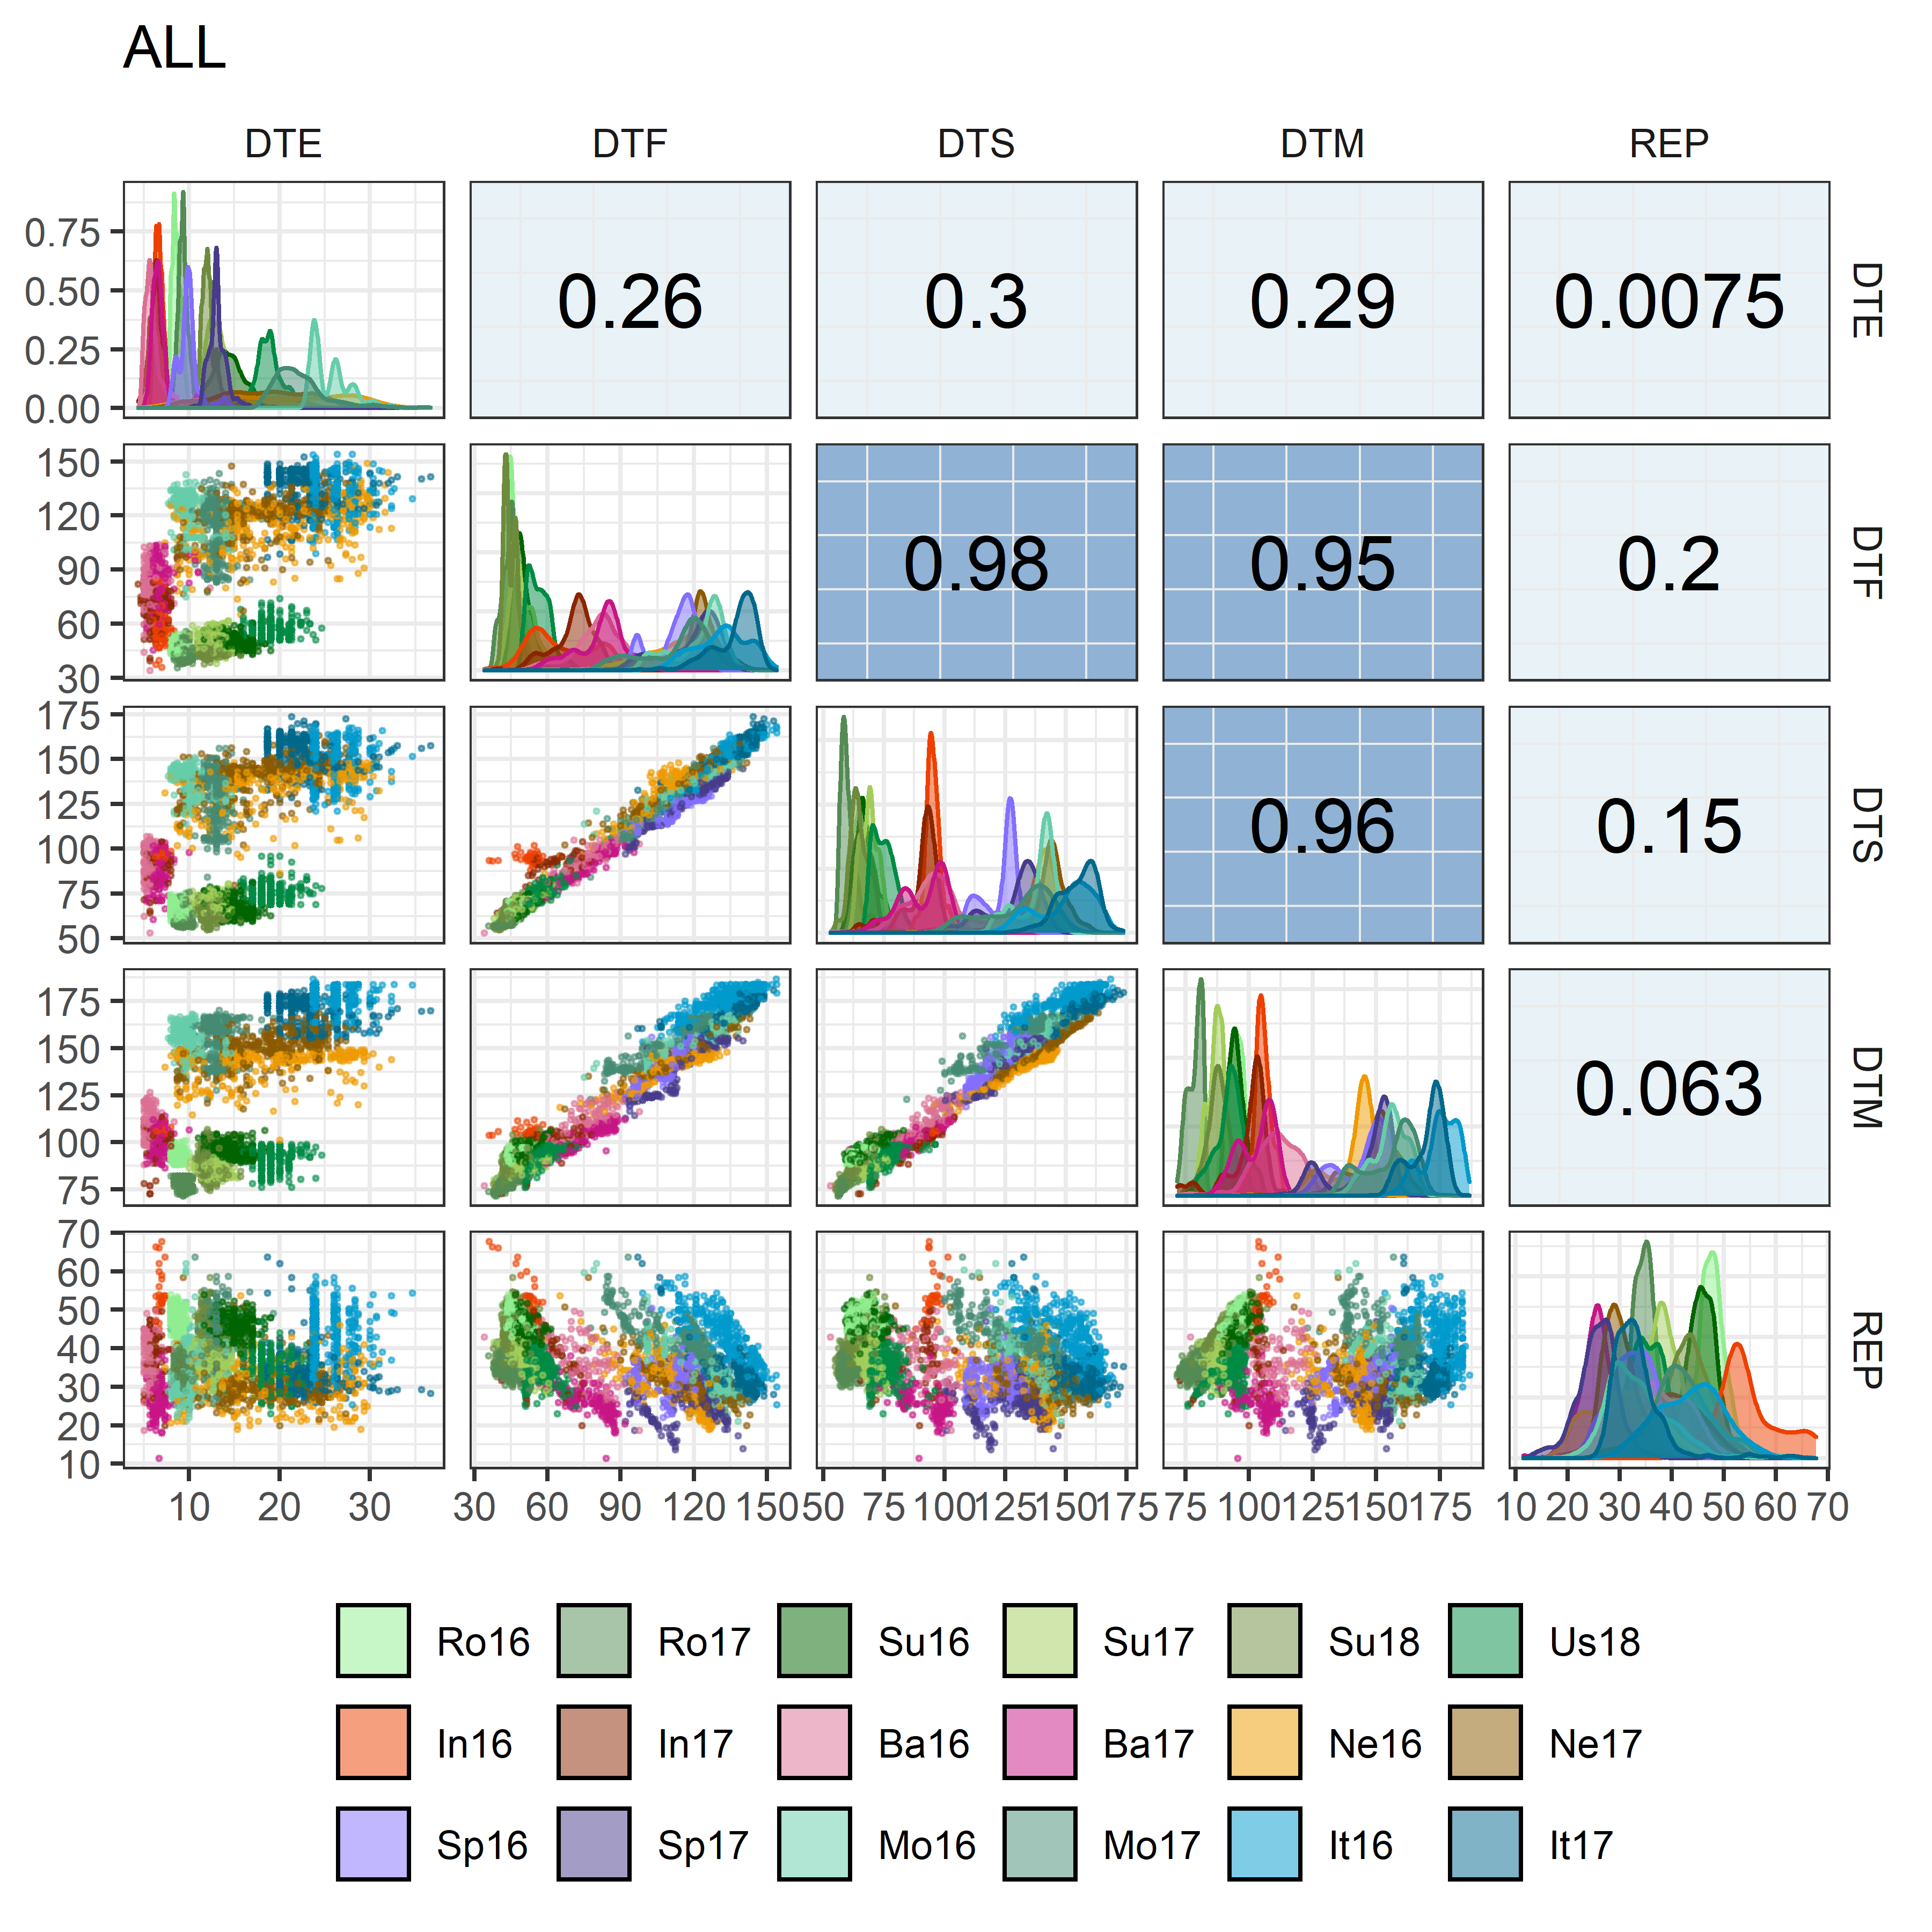
\includegraphics{Additional/Corr/Corr_All.png}

\begin{Shaded}
\begin{Highlighting}[]
\CommentTok{# Prep data}
\NormalTok{xx <-}\StringTok{ }\NormalTok{dd }\OperatorTok\StringTok{ }\KeywordTok{left_join}\NormalTok{(}\KeywordTok{select}\NormalTok{(ff, Expt, MacroEnv), }\DataTypeTok{by =} \StringTok{"Expt"}\NormalTok{) }\OperatorTok
\StringTok{  }\KeywordTok{mutate}\NormalTok{(}\DataTypeTok{DTE =} \KeywordTok{ifelse}\NormalTok{(Location }\OperatorTok{==}\StringTok{ "Cordoba, Spain"}\NormalTok{, }\OtherTok{NA}\NormalTok{, DTE))}
\NormalTok{x1 <-}\StringTok{ }\NormalTok{xx }\OperatorTok\StringTok{ }\KeywordTok{filter}\NormalTok{(MacroEnv }\OperatorTok{==}\StringTok{ "Temperate"}\NormalTok{)}
\NormalTok{x2 <-}\StringTok{ }\NormalTok{xx }\OperatorTok\StringTok{ }\KeywordTok{filter}\NormalTok{(MacroEnv }\OperatorTok{==}\StringTok{ "South Asia"}\NormalTok{)}
\NormalTok{x3 <-}\StringTok{ }\NormalTok{xx }\OperatorTok\StringTok{ }\KeywordTok{filter}\NormalTok{(MacroEnv }\OperatorTok{==}\StringTok{ "Mediterranean"}\NormalTok{)}
\CommentTok{# Create plotting functions}
\NormalTok{my_lower <-}\StringTok{ }\ControlFlowTok{function}\NormalTok{(data, mapping, }\DataTypeTok{cols =}\NormalTok{ colors_Expt, ...) \{}
  \KeywordTok{ggplot}\NormalTok{(}\DataTypeTok{data =}\NormalTok{ data, }\DataTypeTok{mapping =}\NormalTok{ mapping) }\OperatorTok{+}
\StringTok{    }\KeywordTok{geom_point}\NormalTok{(}\DataTypeTok{alpha =} \FloatTok{0.5}\NormalTok{, }\DataTypeTok{size =} \FloatTok{0.3}\NormalTok{, }\KeywordTok{aes}\NormalTok{(}\DataTypeTok{color =}\NormalTok{ Expt)) }\OperatorTok{+}
\StringTok{    }\KeywordTok{theme_bw}\NormalTok{() }\OperatorTok{+}\StringTok{ }
\StringTok{    }\KeywordTok{scale_color_manual}\NormalTok{(}\DataTypeTok{values =}\NormalTok{ cols)}
\NormalTok{\}}
\NormalTok{my_middle <-}\StringTok{ }\ControlFlowTok{function}\NormalTok{(data, mapping, }\DataTypeTok{cols =}\NormalTok{ colors_Expt, ...) \{}
  \KeywordTok{ggplot}\NormalTok{(}\DataTypeTok{data =}\NormalTok{ data, }\DataTypeTok{mapping =}\NormalTok{ mapping) }\OperatorTok{+}\StringTok{ }
\StringTok{    }\KeywordTok{geom_density}\NormalTok{(}\DataTypeTok{alpha =} \FloatTok{0.5}\NormalTok{) }\OperatorTok{+}\StringTok{ }\KeywordTok{theme_bw}\NormalTok{() }\OperatorTok{+}
\StringTok{    }\KeywordTok{scale_color_manual}\NormalTok{(}\DataTypeTok{name =} \OtherTok{NULL}\NormalTok{, }\DataTypeTok{values =}\NormalTok{ cols) }\OperatorTok{+}
\StringTok{    }\KeywordTok{scale_fill_manual}\NormalTok{(}\DataTypeTok{name =} \OtherTok{NULL}\NormalTok{, }\DataTypeTok{values =}\NormalTok{ cols) }\OperatorTok{+}
\StringTok{    }\KeywordTok{guides}\NormalTok{(}\DataTypeTok{color =}\NormalTok{ F, }\DataTypeTok{fill =} \KeywordTok{guide_legend}\NormalTok{(}\DataTypeTok{nrow =} \DecValTok{3}\NormalTok{, }\DataTypeTok{byrow =}\NormalTok{ T))}
\NormalTok{\}}
\CommentTok{# See: https://github.com/ggobi/ggally/issues/139}
\NormalTok{my_upper <-}\StringTok{ }\ControlFlowTok{function}\NormalTok{(data, mapping, }\DataTypeTok{color =} \KeywordTok{I}\NormalTok{(}\StringTok{"black"}\NormalTok{), }\DataTypeTok{sizeRange =} \KeywordTok{c}\NormalTok{(}\DecValTok{1}\NormalTok{,}\DecValTok{5}\NormalTok{), ...) \{}
  \CommentTok{# Prep data}
\NormalTok{  x <-}\StringTok{ }\KeywordTok{eval_data_col}\NormalTok{(data, mapping}\OperatorTok{$}\NormalTok{x) }
\NormalTok{  y <-}\StringTok{ }\KeywordTok{eval_data_col}\NormalTok{(data, mapping}\OperatorTok{$}\NormalTok{y)}
  \CommentTok{#}
\NormalTok{  r2 <-}\StringTok{ }\KeywordTok{cor}\NormalTok{(x, y, }\DataTypeTok{method =} \StringTok{"pearson"}\NormalTok{, }\DataTypeTok{use =} \StringTok{"complete.obs"}\NormalTok{)}\OperatorTok{^}\DecValTok{2}
\NormalTok{  rt <-}\StringTok{ }\KeywordTok{format}\NormalTok{(r2, }\DataTypeTok{digits =} \DecValTok{2}\NormalTok{)[}\DecValTok{1}\NormalTok{]}
\NormalTok{  cex <-}\StringTok{ }\KeywordTok{max}\NormalTok{(sizeRange)}
\NormalTok{  tt <-}\StringTok{ }\KeywordTok{as.character}\NormalTok{(rt)}
  \CommentTok{# plot the cor value}
\NormalTok{  p <-}\StringTok{ }\KeywordTok{ggally_text}\NormalTok{(}\DataTypeTok{label =}\NormalTok{ tt, }\DataTypeTok{mapping =} \KeywordTok{aes}\NormalTok{(), }\DataTypeTok{color =}\NormalTok{ color, }
                   \DataTypeTok{xP =} \FloatTok{0.5}\NormalTok{, }\DataTypeTok{yP =} \FloatTok{0.5}\NormalTok{, }\DataTypeTok{size =} \DecValTok{6}\NormalTok{,  ... ) }\OperatorTok{+}\StringTok{ }\KeywordTok{theme_bw}\NormalTok{() }
  \CommentTok{# Create color palette}
\NormalTok{  corColors <-}\StringTok{ }\NormalTok{RColorBrewer}\OperatorTok{::}\KeywordTok{brewer.pal}\NormalTok{(}\DataTypeTok{n =} \DecValTok{10}\NormalTok{, }\DataTypeTok{name =} \StringTok{"RdBu"}\NormalTok{)[}\DecValTok{2}\OperatorTok{:}\DecValTok{9}\NormalTok{]}
  \ControlFlowTok{if}\NormalTok{        (r2 }\OperatorTok{<=}\StringTok{ }\FloatTok{-0.9}\NormalTok{)              \{ corCol <-}\StringTok{ }\KeywordTok{alpha}\NormalTok{(corColors[}\DecValTok{1}\NormalTok{], }\FloatTok{0.5}\NormalTok{) }
\NormalTok{  \} }\ControlFlowTok{else} \ControlFlowTok{if}\NormalTok{ (r2 }\OperatorTok{>=}\StringTok{ }\FloatTok{-0.9} \OperatorTok{&}\StringTok{ }\NormalTok{r2 }\OperatorTok{<=}\StringTok{ }\FloatTok{-0.6}\NormalTok{) \{ corCol <-}\StringTok{ }\KeywordTok{alpha}\NormalTok{(corColors[}\DecValTok{2}\NormalTok{], }\FloatTok{0.5}\NormalTok{)}
\NormalTok{  \} }\ControlFlowTok{else} \ControlFlowTok{if}\NormalTok{ (r2 }\OperatorTok{>=}\StringTok{ }\FloatTok{-0.6} \OperatorTok{&}\StringTok{ }\NormalTok{r2 }\OperatorTok{<=}\StringTok{ }\FloatTok{-0.3}\NormalTok{) \{ corCol <-}\StringTok{ }\KeywordTok{alpha}\NormalTok{(corColors[}\DecValTok{3}\NormalTok{], }\FloatTok{0.5}\NormalTok{)}
\NormalTok{  \} }\ControlFlowTok{else} \ControlFlowTok{if}\NormalTok{ (r2 }\OperatorTok{>=}\StringTok{ }\FloatTok{-0.3} \OperatorTok{&}\StringTok{ }\NormalTok{r2 }\OperatorTok{<=}\StringTok{ }\DecValTok{0}\NormalTok{)    \{ corCol <-}\StringTok{ }\KeywordTok{alpha}\NormalTok{(corColors[}\DecValTok{4}\NormalTok{], }\FloatTok{0.5}\NormalTok{)}
\NormalTok{  \} }\ControlFlowTok{else} \ControlFlowTok{if}\NormalTok{ (r2 }\OperatorTok{>=}\StringTok{ }\DecValTok{0}    \OperatorTok{&}\StringTok{ }\NormalTok{r2 }\OperatorTok{<=}\StringTok{ }\FloatTok{0.3}\NormalTok{)  \{ corCol <-}\StringTok{ }\KeywordTok{alpha}\NormalTok{(corColors[}\DecValTok{5}\NormalTok{], }\FloatTok{0.5}\NormalTok{) }
\NormalTok{  \} }\ControlFlowTok{else} \ControlFlowTok{if}\NormalTok{ (r2 }\OperatorTok{>=}\StringTok{ }\FloatTok{0.3}  \OperatorTok{&}\StringTok{ }\NormalTok{r2 }\OperatorTok{<=}\StringTok{ }\FloatTok{0.6}\NormalTok{)  \{ corCol <-}\StringTok{ }\KeywordTok{alpha}\NormalTok{(corColors[}\DecValTok{6}\NormalTok{], }\FloatTok{0.5}\NormalTok{)}
\NormalTok{  \} }\ControlFlowTok{else} \ControlFlowTok{if}\NormalTok{ (r2 }\OperatorTok{>=}\StringTok{ }\FloatTok{0.6}  \OperatorTok{&}\StringTok{ }\NormalTok{r2 }\OperatorTok{<=}\StringTok{ }\FloatTok{0.9}\NormalTok{)  \{ corCol <-}\StringTok{ }\KeywordTok{alpha}\NormalTok{(corColors[}\DecValTok{7}\NormalTok{], }\FloatTok{0.5}\NormalTok{) }
\NormalTok{  \} }\ControlFlowTok{else}\NormalTok{                              \{ corCol <-}\StringTok{ }\KeywordTok{alpha}\NormalTok{(corColors[}\DecValTok{8}\NormalTok{], }\FloatTok{0.5}\NormalTok{) \}}
  \CommentTok{# Plot}
\NormalTok{  p <-}\StringTok{ }\NormalTok{p }\OperatorTok{+}
\StringTok{    }\KeywordTok{theme}\NormalTok{(}\DataTypeTok{panel.background =} \KeywordTok{element_rect}\NormalTok{(}\DataTypeTok{fill =}\NormalTok{ corCol),}
          \DataTypeTok{panel.grid.major =} \KeywordTok{element_blank}\NormalTok{(), }
          \CommentTok{#panel.grid.minor = element_blank(),}
          \DataTypeTok{axis.text =} \KeywordTok{element_text}\NormalTok{(}\DataTypeTok{size =} \DecValTok{5}\NormalTok{))}
\NormalTok{  p}
\NormalTok{\}}
\CommentTok{# Plot Correlations for each Expt}
\ControlFlowTok{for}\NormalTok{(i }\ControlFlowTok{in} \DecValTok{1}\OperatorTok{:}\KeywordTok{length}\NormalTok{(names_Expt)) \{}
\NormalTok{  mp <-}\StringTok{ }\KeywordTok{ggpairs}\NormalTok{(xx }\OperatorTok\StringTok{ }\KeywordTok{filter}\NormalTok{(Expt }\OperatorTok{==}\StringTok{ }\NormalTok{names_Expt[i]), }
               \DataTypeTok{columns =} \KeywordTok{c}\NormalTok{(}\StringTok{"DTE"}\NormalTok{, }\StringTok{"DTF"}\NormalTok{, }\StringTok{"DTS"}\NormalTok{, }\StringTok{"DTM"}\NormalTok{, }\StringTok{"REP"}\NormalTok{), }
        \DataTypeTok{upper  =} \KeywordTok{list}\NormalTok{(}\DataTypeTok{continuous =}\NormalTok{ my_upper), }
        \DataTypeTok{diag   =} \KeywordTok{list}\NormalTok{(}\DataTypeTok{continuous =}\NormalTok{ my_middle),}
        \DataTypeTok{lower  =} \KeywordTok{list}\NormalTok{(}\DataTypeTok{continuous =} \KeywordTok{wrap}\NormalTok{(my_lower, }\DataTypeTok{cols =} \StringTok{"black"}\NormalTok{)),}
        \DataTypeTok{title  =}\NormalTok{ i) }\OperatorTok{+}\StringTok{ }
\StringTok{    }\KeywordTok{theme}\NormalTok{(}\DataTypeTok{strip.background =} \KeywordTok{element_rect}\NormalTok{(}\DataTypeTok{fill =} \StringTok{"White"}\NormalTok{))}
  \KeywordTok{ggsave}\NormalTok{(}\KeywordTok{paste0}\NormalTok{(}\StringTok{"Additional/Corr/Corr_"}\NormalTok{, }\KeywordTok{str_pad}\NormalTok{(i, }\DecValTok{2}\NormalTok{, }\StringTok{"left"}\NormalTok{, }\StringTok{"0"}\NormalTok{), }
                \StringTok{"_"}\NormalTok{, names_Expt[i], }\StringTok{".png"}\NormalTok{), }
\NormalTok{         mp, }\DataTypeTok{width =} \DecValTok{6}\NormalTok{, }\DataTypeTok{height =} \DecValTok{6}\NormalTok{, }\DataTypeTok{dpi =} \DecValTok{600}\NormalTok{)}
\NormalTok{\}}
\CommentTok{# Plot (a) Temperate}
\NormalTok{mp1 <-}\StringTok{ }\KeywordTok{ggpairs}\NormalTok{(x1, }\DataTypeTok{columns =} \KeywordTok{c}\NormalTok{(}\StringTok{"DTE"}\NormalTok{, }\StringTok{"DTF"}\NormalTok{, }\StringTok{"DTS"}\NormalTok{, }\StringTok{"DTM"}\NormalTok{, }\StringTok{"REP"}\NormalTok{), }
               \KeywordTok{aes}\NormalTok{(}\DataTypeTok{color =}\NormalTok{ Expt, }\DataTypeTok{fill =}\NormalTok{ Expt),}
        \DataTypeTok{upper=}\KeywordTok{list}\NormalTok{(}\DataTypeTok{continuous =}\NormalTok{ my_upper),}
        \DataTypeTok{diag =}\KeywordTok{list}\NormalTok{(}\DataTypeTok{continuous =} \KeywordTok{wrap}\NormalTok{(my_middle, }\DataTypeTok{cols =}\NormalTok{ colors_Expt[}\DecValTok{1}\OperatorTok{:}\DecValTok{6}\NormalTok{])),}
        \DataTypeTok{lower=}\KeywordTok{list}\NormalTok{(}\DataTypeTok{continuous =} \KeywordTok{wrap}\NormalTok{(my_lower,  }\DataTypeTok{cols =}\NormalTok{ colors_Expt[}\DecValTok{1}\OperatorTok{:}\DecValTok{6}\NormalTok{])),}
        \DataTypeTok{title =} \StringTok{"(a) Temperate"}\NormalTok{, }
        \DataTypeTok{legend =} \KeywordTok{c}\NormalTok{(}\DecValTok{2}\NormalTok{,}\DecValTok{2}\NormalTok{)) }\OperatorTok{+}
\StringTok{  }\KeywordTok{theme}\NormalTok{(}\DataTypeTok{strip.background =} \KeywordTok{element_rect}\NormalTok{(}\DataTypeTok{fill =} \StringTok{"White"}\NormalTok{),}
        \DataTypeTok{legend.position =} \StringTok{"bottom"}\NormalTok{)}
\KeywordTok{ggsave}\NormalTok{(}\StringTok{"Additional/Corr/Corr_Temperate.png"}\NormalTok{, mp1, }\DataTypeTok{width =} \DecValTok{6}\NormalTok{, }\DataTypeTok{height =} \DecValTok{6}\NormalTok{, }\DataTypeTok{dpi =} \DecValTok{600}\NormalTok{)}
\CommentTok{# Plot (b) South Asia}
\NormalTok{mp2 <-}\StringTok{ }\KeywordTok{ggpairs}\NormalTok{(x2, }\DataTypeTok{columns =} \KeywordTok{c}\NormalTok{(}\StringTok{"DTE"}\NormalTok{, }\StringTok{"DTF"}\NormalTok{, }\StringTok{"DTS"}\NormalTok{, }\StringTok{"DTM"}\NormalTok{, }\StringTok{"REP"}\NormalTok{), }
               \KeywordTok{aes}\NormalTok{(}\DataTypeTok{color =}\NormalTok{ Expt, }\DataTypeTok{fill =}\NormalTok{ Expt),}
        \DataTypeTok{upper  =} \KeywordTok{list}\NormalTok{(}\DataTypeTok{continuous =}\NormalTok{ my_upper),}
        \DataTypeTok{diag   =} \KeywordTok{list}\NormalTok{(}\DataTypeTok{continuous =} \KeywordTok{wrap}\NormalTok{(my_middle, }\DataTypeTok{cols =}\NormalTok{ colors_Expt[}\DecValTok{7}\OperatorTok{:}\DecValTok{12}\NormalTok{])),}
        \DataTypeTok{lower  =} \KeywordTok{list}\NormalTok{(}\DataTypeTok{continuous =} \KeywordTok{wrap}\NormalTok{(my_lower,  }\DataTypeTok{cols =}\NormalTok{ colors_Expt[}\DecValTok{7}\OperatorTok{:}\DecValTok{12}\NormalTok{])),}
        \DataTypeTok{title  =} \StringTok{"(b) South Asia"}\NormalTok{, }
        \DataTypeTok{legend =} \KeywordTok{c}\NormalTok{(}\DecValTok{2}\NormalTok{,}\DecValTok{2}\NormalTok{)) }\OperatorTok{+}
\StringTok{  }\KeywordTok{theme}\NormalTok{(}\DataTypeTok{strip.background =} \KeywordTok{element_rect}\NormalTok{(}\DataTypeTok{fill =} \StringTok{"White"}\NormalTok{),}
        \DataTypeTok{legend.position =} \StringTok{"bottom"}\NormalTok{)}
\KeywordTok{ggsave}\NormalTok{(}\StringTok{"Additional/Corr/Corr_SouthAsia.png"}\NormalTok{, mp2, }\DataTypeTok{width =} \DecValTok{6}\NormalTok{, }\DataTypeTok{height =} \DecValTok{6}\NormalTok{, }\DataTypeTok{dpi =} \DecValTok{600}\NormalTok{)}
\CommentTok{# Plot (c) Mediterranean}
\NormalTok{mp3 <-}\StringTok{ }\KeywordTok{ggpairs}\NormalTok{(x3, }\DataTypeTok{columns =} \KeywordTok{c}\NormalTok{(}\StringTok{"DTE"}\NormalTok{, }\StringTok{"DTF"}\NormalTok{, }\StringTok{"DTS"}\NormalTok{, }\StringTok{"DTM"}\NormalTok{, }\StringTok{"REP"}\NormalTok{), }
               \KeywordTok{aes}\NormalTok{(}\DataTypeTok{color =}\NormalTok{ Expt, }\DataTypeTok{fill =}\NormalTok{ Expt),}
        \DataTypeTok{upper  =} \KeywordTok{list}\NormalTok{(}\DataTypeTok{continuous =}\NormalTok{ my_upper),}
        \DataTypeTok{diag   =} \KeywordTok{list}\NormalTok{(}\DataTypeTok{continuous =} \KeywordTok{wrap}\NormalTok{(my_middle, }\DataTypeTok{cols =}\NormalTok{ colors_Expt[}\DecValTok{13}\OperatorTok{:}\DecValTok{18}\NormalTok{])),}
        \DataTypeTok{lower  =} \KeywordTok{list}\NormalTok{(}\DataTypeTok{continuous =} \KeywordTok{wrap}\NormalTok{(my_lower,  }\DataTypeTok{cols =}\NormalTok{ colors_Expt[}\DecValTok{13}\OperatorTok{:}\DecValTok{18}\NormalTok{])),}
        \DataTypeTok{title  =} \StringTok{"(c) Mediterranean"}\NormalTok{, }
        \DataTypeTok{legend =} \KeywordTok{c}\NormalTok{(}\DecValTok{2}\NormalTok{,}\DecValTok{2}\NormalTok{)) }\OperatorTok{+}
\StringTok{  }\KeywordTok{theme}\NormalTok{(}\DataTypeTok{strip.background =} \KeywordTok{element_rect}\NormalTok{(}\DataTypeTok{fill =} \StringTok{"White"}\NormalTok{),}
        \DataTypeTok{legend.position =} \StringTok{"bottom"}\NormalTok{)}
\KeywordTok{ggsave}\NormalTok{(}\StringTok{"Additional/Corr/Corr_Mediterranean.png"}\NormalTok{, mp3, }\DataTypeTok{width =} \DecValTok{6}\NormalTok{, }\DataTypeTok{height =} \DecValTok{6}\NormalTok{, }\DataTypeTok{dpi =} \DecValTok{600}\NormalTok{)}
\CommentTok{# Plot All}
\NormalTok{mp4 <-}\StringTok{ }\KeywordTok{ggpairs}\NormalTok{(xx, }\DataTypeTok{columns =} \KeywordTok{c}\NormalTok{(}\StringTok{"DTE"}\NormalTok{, }\StringTok{"DTF"}\NormalTok{, }\StringTok{"DTS"}\NormalTok{, }\StringTok{"DTM"}\NormalTok{, }\StringTok{"REP"}\NormalTok{), }
        \KeywordTok{aes}\NormalTok{(}\DataTypeTok{color =}\NormalTok{ ExptShort, }\DataTypeTok{fill =}\NormalTok{ ExptShort),}
        \DataTypeTok{upper  =} \KeywordTok{list}\NormalTok{(}\DataTypeTok{continuous =}\NormalTok{ my_upper), }
        \DataTypeTok{diag   =} \KeywordTok{list}\NormalTok{(}\DataTypeTok{continuous =}\NormalTok{ my_middle),}
        \DataTypeTok{lower  =} \KeywordTok{list}\NormalTok{(}\DataTypeTok{continuous =}\NormalTok{ my_lower),}
        \DataTypeTok{title  =} \StringTok{"ALL"}\NormalTok{, }
        \DataTypeTok{legend =} \KeywordTok{c}\NormalTok{(}\DecValTok{2}\NormalTok{,}\DecValTok{2}\NormalTok{)) }\OperatorTok{+}
\StringTok{  }\KeywordTok{theme}\NormalTok{(}\DataTypeTok{strip.background =} \KeywordTok{element_rect}\NormalTok{(}\DataTypeTok{fill =} \StringTok{"White"}\NormalTok{),}
        \DataTypeTok{legend.position =} \StringTok{"bottom"}\NormalTok{)}
\KeywordTok{ggsave}\NormalTok{(}\StringTok{"Additional/Corr/Corr_All.png"}\NormalTok{, mp4, }\DataTypeTok{width =} \DecValTok{6}\NormalTok{, }\DataTypeTok{height =} \DecValTok{6}\NormalTok{, }\DataTypeTok{dpi =} \DecValTok{600}\NormalTok{)}
\end{Highlighting}
\end{Shaded}

\hypertarget{pca}{%
\section{PCA}\label{pca}}

\hypertarget{figure-3-pca}{%
\subsection{Figure 3 PCA}\label{figure-3-pca}}

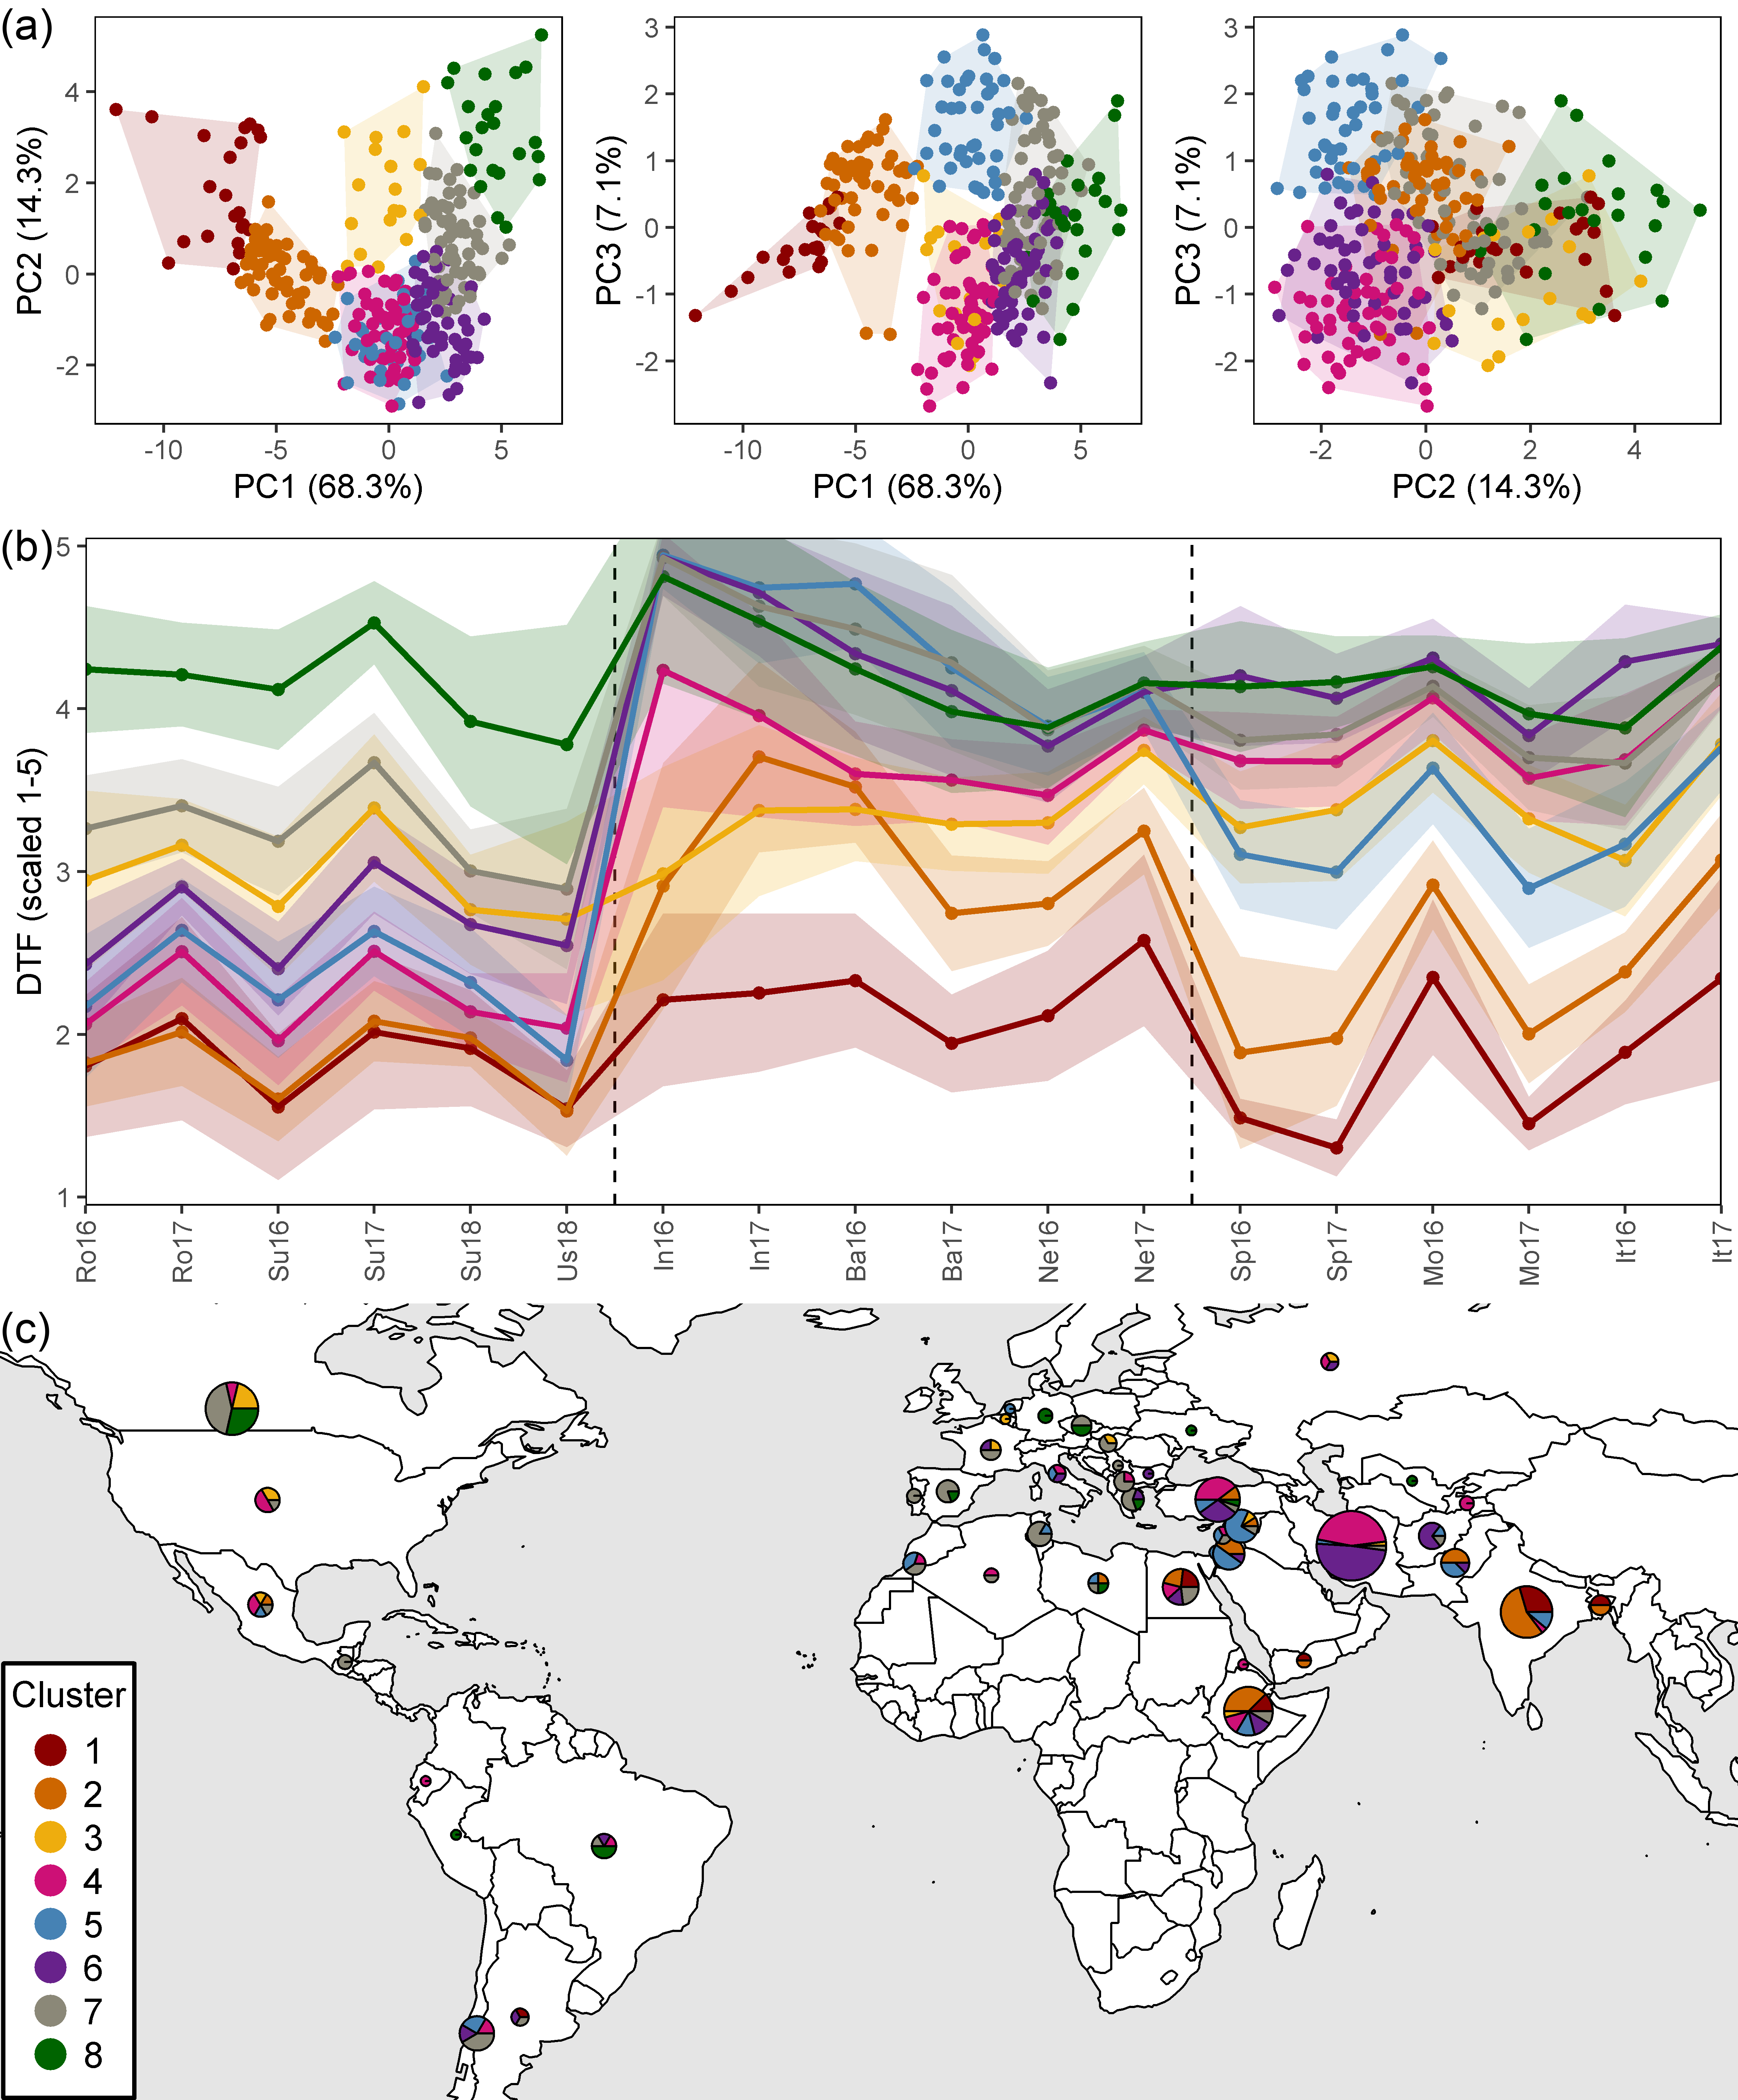
\includegraphics{Figure_03.png}

\begin{Shaded}
\begin{Highlighting}[]
\CommentTok{# Prep data}
\NormalTok{xx <-}\StringTok{ }\NormalTok{dd }\OperatorTok\StringTok{ }\KeywordTok{select}\NormalTok{(Entry, Expt, DTF2_scaled) }\OperatorTok\StringTok{ }
\StringTok{  }\KeywordTok{spread}\NormalTok{(Expt, DTF2_scaled)}
\NormalTok{xx <-}\StringTok{ }\NormalTok{xx }\OperatorTok\StringTok{ }\KeywordTok{column_to_rownames}\NormalTok{(}\StringTok{"Entry"}\NormalTok{) }\OperatorTok\StringTok{ }\KeywordTok{as.matrix}\NormalTok{()}
\CommentTok{# PCA}
\NormalTok{mypca <-}\StringTok{ }\KeywordTok{PCA}\NormalTok{(xx, }\DataTypeTok{ncp =} \DecValTok{10}\NormalTok{, }\DataTypeTok{graph =}\NormalTok{ F)}
\CommentTok{# Heirarcical clustering}
\NormalTok{mypcaH <-}\StringTok{ }\KeywordTok{HCPC}\NormalTok{(mypca, }\DataTypeTok{nb.clust =} \DecValTok{8}\NormalTok{, }\DataTypeTok{graph =}\NormalTok{ F)}
\NormalTok{perc <-}\StringTok{ }\KeywordTok{round}\NormalTok{(mypca[[}\DecValTok{1}\NormalTok{]][,}\DecValTok{2}\NormalTok{], }\DecValTok{1}\NormalTok{)}
\NormalTok{x1}\FloatTok{.1}\NormalTok{ <-}\StringTok{ }\NormalTok{mypcaH[[}\DecValTok{1}\NormalTok{]] }\OperatorTok\StringTok{ }\KeywordTok{rownames_to_column}\NormalTok{(}\StringTok{"Entry"}\NormalTok{)}
\NormalTok{x1}\FloatTok{.2}\NormalTok{ <-}\StringTok{ }\NormalTok{mypca[[}\DecValTok{3}\NormalTok{]]}\OperatorTok{$}\NormalTok{coord }\OperatorTok\StringTok{ }\KeywordTok{as.data.frame}\NormalTok{() }\OperatorTok\StringTok{ }\KeywordTok{rownames_to_column}\NormalTok{(}\StringTok{"Entry"}\NormalTok{)}
\NormalTok{x1 <-}\StringTok{ }\KeywordTok{left_join}\NormalTok{(x1}\FloatTok{.1}\NormalTok{, x1}\FloatTok{.2}\NormalTok{, }\DataTypeTok{by =} \StringTok{"Entry"}\NormalTok{) }\OperatorTok
\StringTok{  }\KeywordTok{mutate}\NormalTok{(}\DataTypeTok{Entry =} \KeywordTok{as.numeric}\NormalTok{(Entry)) }\OperatorTok
\StringTok{  }\KeywordTok{left_join}\NormalTok{(}\KeywordTok{select}\NormalTok{(ldp, Entry, Name, Origin), }\DataTypeTok{by =} \StringTok{"Entry"}\NormalTok{) }\OperatorTok
\StringTok{  }\KeywordTok{left_join}\NormalTok{(}\KeywordTok{select}\NormalTok{(ct, }\DataTypeTok{Origin=}\NormalTok{Country, Region), }\DataTypeTok{by =} \StringTok{"Origin"}\NormalTok{) }\OperatorTok
\StringTok{  }\KeywordTok{select}\NormalTok{(Entry, Name, Origin, Region, }\DataTypeTok{Cluster=}\NormalTok{clust,}
         \DataTypeTok{PC1=}\NormalTok{Dim}\FloatTok{.1}\NormalTok{, }\DataTypeTok{PC2=}\NormalTok{Dim}\FloatTok{.2}\NormalTok{, }\DataTypeTok{PC3=}\NormalTok{Dim}\FloatTok{.3}\NormalTok{, }\DataTypeTok{PC4=}\NormalTok{Dim}\FloatTok{.4}\NormalTok{, }\DataTypeTok{PC5=}\NormalTok{Dim}\FloatTok{.5}\NormalTok{,}
         \DataTypeTok{PC6=}\NormalTok{Dim}\FloatTok{.6}\NormalTok{, }\DataTypeTok{PC7=}\NormalTok{Dim}\FloatTok{.7}\NormalTok{, }\DataTypeTok{PC8=}\NormalTok{Dim}\FloatTok{.8}\NormalTok{, }\DataTypeTok{PC9=}\NormalTok{Dim}\FloatTok{.9}\NormalTok{, }\DataTypeTok{PC10=}\NormalTok{Dim}\FloatTok{.10}\NormalTok{)}
\KeywordTok{write.csv}\NormalTok{(x1, }\StringTok{"data/data_pca_results.csv"}\NormalTok{, }\DataTypeTok{row.names =}\NormalTok{ F)}
\CommentTok{# Prep data}
\NormalTok{x2 <-}\StringTok{ }\NormalTok{dd }\OperatorTok\StringTok{ }\KeywordTok{left_join}\NormalTok{(}\KeywordTok{select}\NormalTok{(x1, Entry, Cluster), }\DataTypeTok{by =} \StringTok{"Entry"}\NormalTok{) }\OperatorTok
\StringTok{  }\KeywordTok{group_by}\NormalTok{(Expt, ExptShort, Cluster) }\OperatorTok\StringTok{ }
\StringTok{  }\KeywordTok{summarise}\NormalTok{(}\DataTypeTok{mean =} \KeywordTok{mean}\NormalTok{(DTF2_scaled, }\DataTypeTok{na.rm =}\NormalTok{ T), }\DataTypeTok{sd =} \KeywordTok{sd}\NormalTok{(DTF2_scaled, }\DataTypeTok{na.rm =}\NormalTok{ T)) }\OperatorTok
\StringTok{  }\KeywordTok{ungroup}\NormalTok{() }\OperatorTok
\StringTok{  }\KeywordTok{mutate}\NormalTok{(}\DataTypeTok{ClusterNum =}\NormalTok{ plyr}\OperatorTok{::}\KeywordTok{mapvalues}\NormalTok{(Cluster, }\KeywordTok{as.character}\NormalTok{(}\DecValTok{1}\OperatorTok{:}\DecValTok{8}\NormalTok{), }\KeywordTok{summary}\NormalTok{(x1}\OperatorTok{$}\NormalTok{Cluster)))}
\NormalTok{x3 <-}\StringTok{ }\NormalTok{x1 }\OperatorTok\StringTok{ }\KeywordTok{count}\NormalTok{(Cluster) }\OperatorTok\StringTok{ }
\StringTok{  }\KeywordTok{mutate}\NormalTok{(}\DataTypeTok{Cluster =} \KeywordTok{factor}\NormalTok{(Cluster, }\DataTypeTok{levels =} \KeywordTok{rev}\NormalTok{(}\KeywordTok{levels}\NormalTok{(Cluster))), }\DataTypeTok{y =}\NormalTok{ n}\OperatorTok{/}\DecValTok{2}\NormalTok{)}
\ControlFlowTok{for}\NormalTok{(i }\ControlFlowTok{in} \DecValTok{2}\OperatorTok{:}\KeywordTok{nrow}\NormalTok{(x3)) \{ x3}\OperatorTok{$}\NormalTok{y[i] <-}\StringTok{ }\KeywordTok{sum}\NormalTok{(x3}\OperatorTok{$}\NormalTok{n[}\DecValTok{1}\OperatorTok{:}\NormalTok{(i}\DecValTok{-1}\NormalTok{)]) }\OperatorTok{+}\StringTok{ }\NormalTok{(x3}\OperatorTok{$}\NormalTok{n[i]}\OperatorTok{/}\DecValTok{2}\NormalTok{) \}}
\CommentTok{# Plot (a) PCA 1v2}
\NormalTok{find_hull <-}\StringTok{ }\ControlFlowTok{function}\NormalTok{(df) df[}\KeywordTok{chull}\NormalTok{(df[,}\StringTok{"PC1"}\NormalTok{], df[,}\StringTok{"PC2"}\NormalTok{]), ]}
\NormalTok{polys <-}\StringTok{ }\NormalTok{plyr}\OperatorTok{::}\KeywordTok{ddply}\NormalTok{(x1, }\StringTok{"Cluster"}\NormalTok{, find_hull) }\OperatorTok\StringTok{ }\KeywordTok{mutate}\NormalTok{(}\DataTypeTok{Cluster =} \KeywordTok{factor}\NormalTok{(Cluster))}
\NormalTok{mp1}\FloatTok{.1}\NormalTok{ <-}\StringTok{ }\KeywordTok{ggplot}\NormalTok{(x1) }\OperatorTok{+}
\StringTok{  }\KeywordTok{geom_polygon}\NormalTok{(}\DataTypeTok{data =}\NormalTok{ polys, }\DataTypeTok{alpha =} \FloatTok{0.15}\NormalTok{, }\KeywordTok{aes}\NormalTok{(}\DataTypeTok{x =}\NormalTok{ PC1, }\DataTypeTok{y =}\NormalTok{ PC2, }\DataTypeTok{fill =}\NormalTok{ Cluster)) }\OperatorTok{+}
\StringTok{  }\KeywordTok{geom_point}\NormalTok{(}\KeywordTok{aes}\NormalTok{(}\DataTypeTok{x =}\NormalTok{ PC1, }\DataTypeTok{y =}\NormalTok{ PC2, }\DataTypeTok{colour =}\NormalTok{ Cluster)) }\OperatorTok{+}
\StringTok{  }\KeywordTok{scale_fill_manual}\NormalTok{(}\DataTypeTok{values =}\NormalTok{ colors) }\OperatorTok{+}
\StringTok{  }\KeywordTok{scale_color_manual}\NormalTok{(}\DataTypeTok{values =}\NormalTok{ colors) }\OperatorTok{+}
\StringTok{  }\NormalTok{theme_AGL }\OperatorTok{+}\StringTok{ }
\StringTok{  }\KeywordTok{theme}\NormalTok{(}\DataTypeTok{legend.position =} \StringTok{"none"}\NormalTok{, }\DataTypeTok{panel.grid =} \KeywordTok{element_blank}\NormalTok{()) }\OperatorTok{+}
\StringTok{  }\KeywordTok{labs}\NormalTok{(}\DataTypeTok{x =} \KeywordTok{paste0}\NormalTok{(}\StringTok{"PC1 ("}\NormalTok{, perc[}\DecValTok{1}\NormalTok{], }\StringTok{"%)"}\NormalTok{),}
       \DataTypeTok{y =} \KeywordTok{paste0}\NormalTok{(}\StringTok{"PC2 ("}\NormalTok{, perc[}\DecValTok{2}\NormalTok{], }\StringTok{"%)"}\NormalTok{))}
\CommentTok{# Plot (a) PCA 1v3}
\NormalTok{find_hull <-}\StringTok{ }\ControlFlowTok{function}\NormalTok{(df) df[}\KeywordTok{chull}\NormalTok{(df[,}\StringTok{"PC1"}\NormalTok{], df[,}\StringTok{"PC3"}\NormalTok{]), ]}
\NormalTok{polys <-}\StringTok{ }\NormalTok{plyr}\OperatorTok{::}\KeywordTok{ddply}\NormalTok{(x1, }\StringTok{"Cluster"}\NormalTok{, find_hull) }\OperatorTok\StringTok{ }\KeywordTok{mutate}\NormalTok{(}\DataTypeTok{Cluster =} \KeywordTok{factor}\NormalTok{(Cluster))}
\NormalTok{mp1}\FloatTok{.2}\NormalTok{ <-}\StringTok{ }\KeywordTok{ggplot}\NormalTok{(x1) }\OperatorTok{+}
\StringTok{  }\KeywordTok{geom_polygon}\NormalTok{(}\DataTypeTok{data =}\NormalTok{ polys, }\DataTypeTok{alpha =} \FloatTok{0.15}\NormalTok{, }\KeywordTok{aes}\NormalTok{(}\DataTypeTok{x =}\NormalTok{ PC1, }\DataTypeTok{y =}\NormalTok{ PC3, }\DataTypeTok{fill =}\NormalTok{ Cluster)) }\OperatorTok{+}
\StringTok{  }\KeywordTok{geom_point}\NormalTok{(}\KeywordTok{aes}\NormalTok{(}\DataTypeTok{x =}\NormalTok{ PC1, }\DataTypeTok{y =}\NormalTok{ PC3, }\DataTypeTok{colour =}\NormalTok{ Cluster)) }\OperatorTok{+}
\StringTok{  }\KeywordTok{scale_fill_manual}\NormalTok{(}\DataTypeTok{values =}\NormalTok{ colors) }\OperatorTok{+}
\StringTok{  }\KeywordTok{scale_color_manual}\NormalTok{(}\DataTypeTok{values =}\NormalTok{ colors) }\OperatorTok{+}
\StringTok{  }\NormalTok{theme_AGL }\OperatorTok{+}\StringTok{ }
\StringTok{  }\KeywordTok{theme}\NormalTok{(}\DataTypeTok{legend.position =} \StringTok{"none"}\NormalTok{, }\DataTypeTok{panel.grid =} \KeywordTok{element_blank}\NormalTok{()) }\OperatorTok{+}
\StringTok{  }\KeywordTok{labs}\NormalTok{(}\DataTypeTok{x =} \KeywordTok{paste0}\NormalTok{(}\StringTok{"PC1 ("}\NormalTok{, perc[}\DecValTok{1}\NormalTok{], }\StringTok{"%)"}\NormalTok{),}
       \DataTypeTok{y =} \KeywordTok{paste0}\NormalTok{(}\StringTok{"PC3 ("}\NormalTok{, perc[}\DecValTok{3}\NormalTok{], }\StringTok{"%)"}\NormalTok{))}
\CommentTok{# Plot (a) PCA 2v3}
\NormalTok{find_hull <-}\StringTok{ }\ControlFlowTok{function}\NormalTok{(df) df[}\KeywordTok{chull}\NormalTok{(df[,}\StringTok{"PC2"}\NormalTok{], df[,}\StringTok{"PC3"}\NormalTok{]), ]}
\NormalTok{polys <-}\StringTok{ }\NormalTok{plyr}\OperatorTok{::}\KeywordTok{ddply}\NormalTok{(x1, }\StringTok{"Cluster"}\NormalTok{, find_hull) }\OperatorTok\StringTok{ }\KeywordTok{mutate}\NormalTok{(}\DataTypeTok{Cluster =} \KeywordTok{factor}\NormalTok{(Cluster))}
\NormalTok{mp1}\FloatTok{.3}\NormalTok{ <-}\StringTok{ }\KeywordTok{ggplot}\NormalTok{(x1) }\OperatorTok{+}
\StringTok{  }\KeywordTok{geom_polygon}\NormalTok{(}\DataTypeTok{data =}\NormalTok{ polys, }\DataTypeTok{alpha =} \FloatTok{0.15}\NormalTok{, }\KeywordTok{aes}\NormalTok{(}\DataTypeTok{x =}\NormalTok{ PC2, }\DataTypeTok{y =}\NormalTok{ PC3, }\DataTypeTok{fill =}\NormalTok{ Cluster)) }\OperatorTok{+}
\StringTok{  }\KeywordTok{geom_point}\NormalTok{(}\KeywordTok{aes}\NormalTok{(}\DataTypeTok{x =}\NormalTok{ PC2, }\DataTypeTok{y =}\NormalTok{ PC3, }\DataTypeTok{colour =}\NormalTok{ Cluster)) }\OperatorTok{+}
\StringTok{  }\KeywordTok{scale_fill_manual}\NormalTok{(}\DataTypeTok{values =}\NormalTok{ colors) }\OperatorTok{+}
\StringTok{  }\KeywordTok{scale_color_manual}\NormalTok{(}\DataTypeTok{values =}\NormalTok{ colors) }\OperatorTok{+}
\StringTok{  }\NormalTok{theme_AGL }\OperatorTok{+}\StringTok{ }
\StringTok{  }\KeywordTok{theme}\NormalTok{(}\DataTypeTok{legend.position =} \StringTok{"none"}\NormalTok{, }\DataTypeTok{panel.grid =} \KeywordTok{element_blank}\NormalTok{()) }\OperatorTok{+}
\StringTok{  }\KeywordTok{labs}\NormalTok{(}\DataTypeTok{x =} \KeywordTok{paste0}\NormalTok{(}\StringTok{"PC2 ("}\NormalTok{, perc[}\DecValTok{2}\NormalTok{], }\StringTok{"%)"}\NormalTok{),}
       \DataTypeTok{y =} \KeywordTok{paste0}\NormalTok{(}\StringTok{"PC3 ("}\NormalTok{, perc[}\DecValTok{3}\NormalTok{], }\StringTok{"%)"}\NormalTok{))}
\CommentTok{# Append }
\NormalTok{mp1 <-}\StringTok{ }\KeywordTok{ggarrange}\NormalTok{(mp1}\FloatTok{.1}\NormalTok{, mp1}\FloatTok{.2}\NormalTok{, mp1}\FloatTok{.3}\NormalTok{, }\DataTypeTok{nrow =} \DecValTok{1}\NormalTok{, }\DataTypeTok{ncol =} \DecValTok{3}\NormalTok{, }\DataTypeTok{hjust =} \DecValTok{0}\NormalTok{)}
\CommentTok{# Plot (b) DTF }
\NormalTok{mp2 <-}\StringTok{ }\KeywordTok{ggplot}\NormalTok{(x2, }\KeywordTok{aes}\NormalTok{(}\DataTypeTok{x =}\NormalTok{ ExptShort, }\DataTypeTok{y =}\NormalTok{ mean, }\DataTypeTok{group =}\NormalTok{ Cluster)) }\OperatorTok{+}
\StringTok{  }\KeywordTok{geom_point}\NormalTok{(}\KeywordTok{aes}\NormalTok{(}\DataTypeTok{color =}\NormalTok{ Cluster)) }\OperatorTok{+}\StringTok{ }
\StringTok{  }\KeywordTok{geom_vline}\NormalTok{(}\DataTypeTok{xintercept =} \FloatTok{6.5}\NormalTok{,  }\DataTypeTok{lty =} \DecValTok{2}\NormalTok{) }\OperatorTok{+}\StringTok{ }
\StringTok{  }\KeywordTok{geom_vline}\NormalTok{(}\DataTypeTok{xintercept =} \FloatTok{12.5}\NormalTok{, }\DataTypeTok{lty =} \DecValTok{2}\NormalTok{) }\OperatorTok{+}
\StringTok{  }\KeywordTok{geom_ribbon}\NormalTok{(}\KeywordTok{aes}\NormalTok{(}\DataTypeTok{ymin =}\NormalTok{ mean }\OperatorTok{-}\StringTok{ }\NormalTok{sd, }\DataTypeTok{ymax =}\NormalTok{ mean }\OperatorTok{+}\StringTok{ }\NormalTok{sd, }\DataTypeTok{fill =}\NormalTok{ Cluster), }
              \DataTypeTok{alpha =} \FloatTok{0.2}\NormalTok{, }\DataTypeTok{color =} \OtherTok{NA}\NormalTok{) }\OperatorTok{+}\StringTok{ }
\StringTok{  }\KeywordTok{geom_line}\NormalTok{(}\KeywordTok{aes}\NormalTok{(}\DataTypeTok{color =}\NormalTok{ Cluster), }\DataTypeTok{size =} \DecValTok{1}\NormalTok{) }\OperatorTok{+}
\StringTok{  }\KeywordTok{scale_color_manual}\NormalTok{(}\DataTypeTok{values =}\NormalTok{ colors) }\OperatorTok{+}
\StringTok{  }\KeywordTok{scale_fill_manual}\NormalTok{(}\DataTypeTok{values =}\NormalTok{ colors) }\OperatorTok{+}
\StringTok{  }\KeywordTok{coord_cartesian}\NormalTok{(}\DataTypeTok{ylim =} \KeywordTok{c}\NormalTok{(}\FloatTok{0.95}\NormalTok{,}\FloatTok{5.05}\NormalTok{), }\DataTypeTok{expand =}\NormalTok{ F) }\OperatorTok{+}
\StringTok{  }\NormalTok{theme_AGL }\OperatorTok{+}
\StringTok{  }\KeywordTok{theme}\NormalTok{(}\DataTypeTok{axis.text.x =} \KeywordTok{element_text}\NormalTok{(}\DataTypeTok{angle =} \DecValTok{90}\NormalTok{, }\DataTypeTok{hjust =} \DecValTok{1}\NormalTok{, }\DataTypeTok{vjust =} \FloatTok{0.5}\NormalTok{),}
        \DataTypeTok{legend.position =} \StringTok{"none"}\NormalTok{, }\DataTypeTok{panel.grid =} \KeywordTok{element_blank}\NormalTok{()) }\OperatorTok{+}\StringTok{ }
\StringTok{  }\KeywordTok{labs}\NormalTok{(}\DataTypeTok{y =} \StringTok{"DTF (scaled 1-5)"}\NormalTok{, }\DataTypeTok{x =} \OtherTok{NULL}\NormalTok{)}
\CommentTok{#}
\KeywordTok{ggsave}\NormalTok{(}\StringTok{"Additional/Temp/Temp_F03_1.png"}\NormalTok{, mp1, }\DataTypeTok{width =} \DecValTok{8}\NormalTok{, }\DataTypeTok{height =}   \DecValTok{1}\OperatorTok{*}\DecValTok{6}\OperatorTok{/}\FloatTok{2.5}\NormalTok{, }\DataTypeTok{dpi =} \DecValTok{600}\NormalTok{)}
\KeywordTok{ggsave}\NormalTok{(}\StringTok{"Additional/Temp/Temp_F03_2.png"}\NormalTok{, mp2, }\DataTypeTok{width =} \DecValTok{8}\NormalTok{, }\DataTypeTok{height =} \FloatTok{1.5}\OperatorTok{*}\DecValTok{6}\OperatorTok{/}\FloatTok{2.5}\NormalTok{, }\DataTypeTok{dpi =} \DecValTok{600}\NormalTok{)}
\CommentTok{# Plot (c)}
\NormalTok{xx <-}\StringTok{ }\NormalTok{ldp }\OperatorTok\StringTok{ }\KeywordTok{left_join}\NormalTok{(}\KeywordTok{select}\NormalTok{(x1, Entry, Cluster), }\DataTypeTok{by =} \StringTok{"Entry"}\NormalTok{) }\OperatorTok
\StringTok{  }\KeywordTok{mutate}\NormalTok{(}\DataTypeTok{test1 =} \KeywordTok{factor}\NormalTok{(}\KeywordTok{paste}\NormalTok{(Origin, Cluster)))}
\NormalTok{xx <-}\StringTok{ }\NormalTok{xx }\OperatorTok\StringTok{ }\KeywordTok{filter}\NormalTok{(}\OperatorTok{!}\NormalTok{Origin }\OperatorTok\StringTok{ }\KeywordTok{c}\NormalTok{(}\StringTok{"ICARDA"}\NormalTok{,}\StringTok{"USDA"}\NormalTok{,}\StringTok{"Unknown"}\NormalTok{)) }\OperatorTok\StringTok{ }
\StringTok{  }\KeywordTok{group_by}\NormalTok{(Origin, Cluster) }\OperatorTok\StringTok{ }\KeywordTok{summarise}\NormalTok{(}\DataTypeTok{Count =} \KeywordTok{n}\NormalTok{()) }\OperatorTok\StringTok{ }
\StringTok{  }\KeywordTok{spread}\NormalTok{(Cluster, Count) }\OperatorTok
\StringTok{  }\KeywordTok{left_join}\NormalTok{(}\KeywordTok{select}\NormalTok{(ct, }\DataTypeTok{Origin=}\NormalTok{Country, Lat, Lon), }\DataTypeTok{by =} \StringTok{"Origin"}\NormalTok{) }\OperatorTok\StringTok{ }
\StringTok{  }\KeywordTok{ungroup}\NormalTok{() }\OperatorTok\StringTok{ }\KeywordTok{as.data.frame}\NormalTok{()}
\NormalTok{xx[}\KeywordTok{is.na}\NormalTok{(xx)] <-}\StringTok{ }\DecValTok{0} 
\KeywordTok{invisible}\NormalTok{(}\KeywordTok{png}\NormalTok{(}\StringTok{"Additional/Temp/Temp_F03_3.png"}\NormalTok{, }\DataTypeTok{width =} \DecValTok{4800}\NormalTok{, }\DataTypeTok{height =} \DecValTok{2200}\NormalTok{, }\DataTypeTok{res =} \DecValTok{600}\NormalTok{))}
\KeywordTok{par}\NormalTok{(}\DataTypeTok{mai =} \KeywordTok{c}\NormalTok{(}\DecValTok{0}\NormalTok{,}\DecValTok{0}\NormalTok{,}\DecValTok{0}\NormalTok{,}\DecValTok{0}\NormalTok{), }\DataTypeTok{xaxs =} \StringTok{"i"}\NormalTok{, }\DataTypeTok{yaxs =} \StringTok{"i"}\NormalTok{)}
\KeywordTok{mapPies}\NormalTok{(}\DataTypeTok{dF =}\NormalTok{ xx, }\DataTypeTok{nameX =} \StringTok{"Lon"}\NormalTok{, }\DataTypeTok{nameY =} \StringTok{"Lat"}\NormalTok{, }\DataTypeTok{zColours =}\NormalTok{ colors,}
        \DataTypeTok{nameZs =} \KeywordTok{c}\NormalTok{(}\StringTok{"1"}\NormalTok{,}\StringTok{"2"}\NormalTok{,}\StringTok{"3"}\NormalTok{,}\StringTok{"4"}\NormalTok{,}\StringTok{"5"}\NormalTok{,}\StringTok{"6"}\NormalTok{,}\StringTok{"7"}\NormalTok{,}\StringTok{"8"}\NormalTok{), }\DataTypeTok{lwd =} \DecValTok{1}\NormalTok{,}
        \DataTypeTok{xlim =} \KeywordTok{c}\NormalTok{(}\OperatorTok{-}\DecValTok{140}\NormalTok{,}\DecValTok{110}\NormalTok{), }\DataTypeTok{ylim =} \KeywordTok{c}\NormalTok{(}\DecValTok{0}\NormalTok{,}\DecValTok{20}\NormalTok{), }\DataTypeTok{addCatLegend =}\NormalTok{ F,}
        \DataTypeTok{oceanCol =} \StringTok{"grey90"}\NormalTok{, }\DataTypeTok{landCol =} \StringTok{"white"}\NormalTok{, }\DataTypeTok{borderCol =} \StringTok{"black"}\NormalTok{) }
\end{Highlighting}
\end{Shaded}

\begin{verbatim}
symbolMaxSize= 5  maxSumValues= 49  symbolScale= 0.7142857 
List of 2
 $ x: num [1:100] -125 -125 -125 -125 -125 ...
 $ y: num [1:100] 57.3 57.6 57.9 58.2 58.5 ...
\end{verbatim}

\begin{Shaded}
\begin{Highlighting}[]
\KeywordTok{legend}\NormalTok{(}\OperatorTok{-}\FloatTok{139.5}\NormalTok{, }\FloatTok{15.5}\NormalTok{, }\DataTypeTok{title =} \StringTok{"Cluster"}\NormalTok{, }\DataTypeTok{legend =} \DecValTok{1}\OperatorTok{:}\DecValTok{8}\NormalTok{, }\DataTypeTok{col =}\NormalTok{ colors,}
       \DataTypeTok{pch =} \DecValTok{16}\NormalTok{, }\DataTypeTok{cex =} \DecValTok{1}\NormalTok{, }\DataTypeTok{pt.cex =} \DecValTok{2}\NormalTok{, }\DataTypeTok{box.lwd =} \DecValTok{2}\NormalTok{)}
\KeywordTok{invisible}\NormalTok{(}\KeywordTok{dev.off}\NormalTok{())}
\CommentTok{# Append (a), (b) and (c)}
\NormalTok{im1 <-}\StringTok{ }\KeywordTok{image_read}\NormalTok{(}\StringTok{"Additional/Temp/Temp_F03_1.png"}\NormalTok{) }\OperatorTok\StringTok{ }
\StringTok{  }\KeywordTok{image_annotate}\NormalTok{(}\StringTok{"(a)"}\NormalTok{, }\DataTypeTok{size =} \DecValTok{120}\NormalTok{, }\DataTypeTok{location =} \StringTok{"+0+0"}\NormalTok{)}
\NormalTok{im2 <-}\StringTok{ }\KeywordTok{image_read}\NormalTok{(}\StringTok{"Additional/Temp/Temp_F03_2.png"}\NormalTok{) }\OperatorTok\StringTok{ }
\StringTok{  }\KeywordTok{image_annotate}\NormalTok{(}\StringTok{"(b)"}\NormalTok{, }\DataTypeTok{size =} \DecValTok{120}\NormalTok{, }\DataTypeTok{location =} \StringTok{"+0+0"}\NormalTok{)}
\NormalTok{im3 <-}\StringTok{ }\KeywordTok{image_read}\NormalTok{(}\StringTok{"Additional/Temp/Temp_F03_3.png"}\NormalTok{) }\OperatorTok
\StringTok{  }\KeywordTok{image_annotate}\NormalTok{(}\StringTok{"(c)"}\NormalTok{, }\DataTypeTok{size =} \DecValTok{120}\NormalTok{, }\DataTypeTok{location =} \StringTok{"+0+0"}\NormalTok{)}
\NormalTok{im <-}\StringTok{ }\KeywordTok{image_append}\NormalTok{(}\KeywordTok{c}\NormalTok{(im1, im2, im3), }\DataTypeTok{stack =}\NormalTok{ T)}
\KeywordTok{image_write}\NormalTok{(im, }\StringTok{"Figure_03.png"}\NormalTok{)}
\end{Highlighting}
\end{Shaded}

\hypertarget{additional-figure-5-interactive-pca-plot}{%
\subsection{Additional Figure 5 Interactive PCA
Plot}\label{additional-figure-5-interactive-pca-plot}}

\begin{Shaded}
\begin{Highlighting}[]
\NormalTok{pca <-}\StringTok{ }\KeywordTok{read.csv}\NormalTok{(}\StringTok{"data/data_pca_results.csv"}\NormalTok{) }\OperatorTok\StringTok{ }
\StringTok{  }\KeywordTok{mutate}\NormalTok{(}\DataTypeTok{Cluster =} \KeywordTok{factor}\NormalTok{(Cluster),}
         \DataTypeTok{myColors =}\NormalTok{ plyr}\OperatorTok{::}\KeywordTok{mapvalues}\NormalTok{(Cluster, }\DecValTok{1}\OperatorTok{:}\DecValTok{8}\NormalTok{, colors))}
\NormalTok{rgl}\OperatorTok{::}\KeywordTok{plot3d}\NormalTok{(pca[,}\DecValTok{5}\OperatorTok{:}\DecValTok{7}\NormalTok{], }\DataTypeTok{col =}\NormalTok{ pca}\OperatorTok{$}\NormalTok{myColors, }\DataTypeTok{size =} \DecValTok{15}\NormalTok{)}
\NormalTok{rgl}\OperatorTok{::}\KeywordTok{writeWebGL}\NormalTok{(}\DataTypeTok{filename =} \StringTok{"Additional/Additional_Figure_05.html"}\NormalTok{, }
                \DataTypeTok{width =} \DecValTok{650}\NormalTok{, }\DataTypeTok{height =} \DecValTok{650}\NormalTok{)}
\end{Highlighting}
\end{Shaded}

\hypertarget{additional-figure-6-pca}{%
\subsection{Additional Figure 6 PCA}\label{additional-figure-6-pca}}

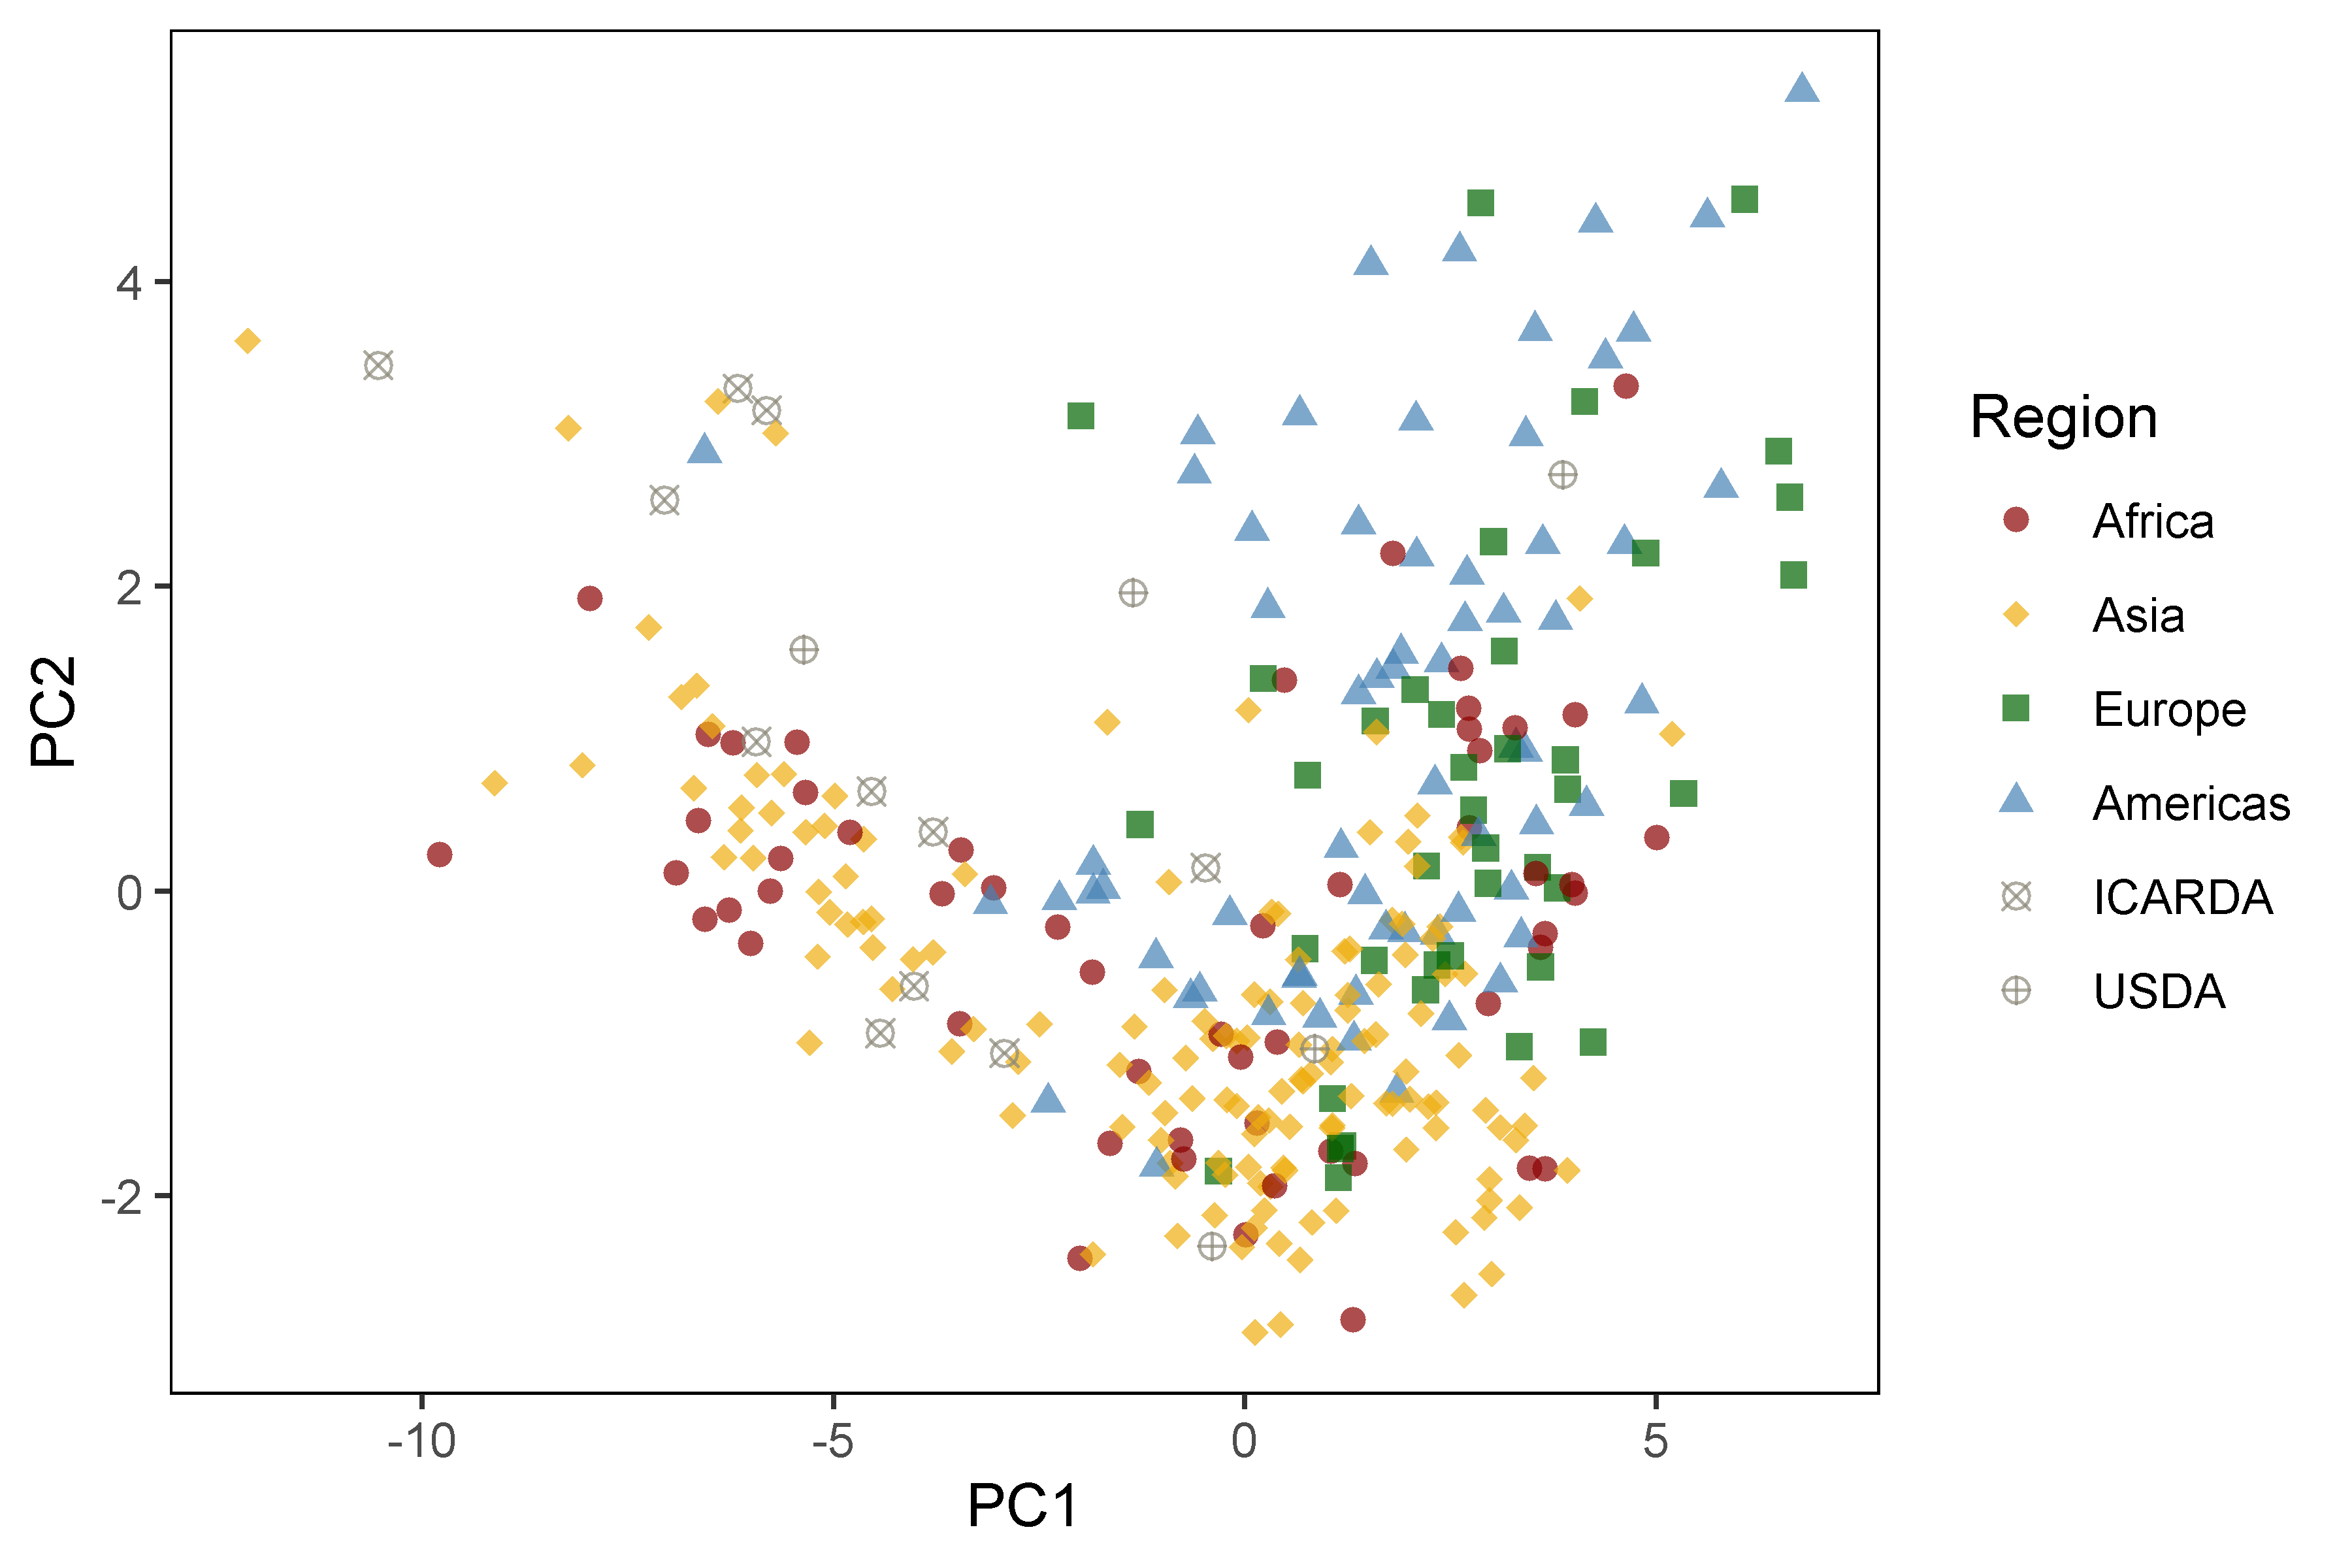
\includegraphics{Additional/Additional_Figure_06.png}

\begin{Shaded}
\begin{Highlighting}[]
\CommentTok{# Prep data}
\NormalTok{levs <-}\StringTok{ }\KeywordTok{c}\NormalTok{(}\StringTok{"Africa"}\NormalTok{, }\StringTok{"Asia"}\NormalTok{, }\StringTok{"Europe"}\NormalTok{, }\StringTok{"Americas"}\NormalTok{, }\StringTok{"ICARDA"}\NormalTok{, }\StringTok{"USDA"}\NormalTok{)}
\NormalTok{xx <-}\StringTok{ }\KeywordTok{read.csv}\NormalTok{(}\StringTok{"data/data_pca_results.csv"}\NormalTok{) }\OperatorTok\StringTok{ }
\StringTok{  }\KeywordTok{filter}\NormalTok{(Origin }\OperatorTok{!=}\StringTok{ "Unknown"}\NormalTok{) }\OperatorTok
\StringTok{  }\KeywordTok{mutate}\NormalTok{(}\DataTypeTok{Region =} \KeywordTok{as.character}\NormalTok{(Region), }\DataTypeTok{Origin =} \KeywordTok{as.character}\NormalTok{(Origin),}
         \DataTypeTok{Region =} \KeywordTok{ifelse}\NormalTok{(Origin }\OperatorTok\StringTok{ }\NormalTok{levs[}\DecValTok{5}\OperatorTok{:}\DecValTok{6}\NormalTok{], Origin, Region),}
         \DataTypeTok{Region =} \KeywordTok{factor}\NormalTok{(Region, }\DataTypeTok{levels =}\NormalTok{ levs))}
\CommentTok{# Plot}
\NormalTok{mp <-}\StringTok{ }\KeywordTok{ggplot}\NormalTok{(xx, }\KeywordTok{aes}\NormalTok{(}\DataTypeTok{x =}\NormalTok{ PC1, }\DataTypeTok{y =}\NormalTok{ PC2, }\DataTypeTok{color =}\NormalTok{ Region, }\DataTypeTok{shape =}\NormalTok{ Region)) }\OperatorTok{+}
\StringTok{  }\KeywordTok{geom_point}\NormalTok{(}\DataTypeTok{alpha =} \FloatTok{0.7}\NormalTok{, }\DataTypeTok{size =} \DecValTok{2}\NormalTok{) }\OperatorTok{+}
\StringTok{  }\KeywordTok{scale_color_manual}\NormalTok{(}\DataTypeTok{values =}\NormalTok{ colors[}\KeywordTok{c}\NormalTok{(}\DecValTok{1}\NormalTok{,}\DecValTok{3}\NormalTok{,}\DecValTok{8}\NormalTok{,}\DecValTok{5}\NormalTok{,}\DecValTok{7}\NormalTok{,}\DecValTok{7}\NormalTok{)]) }\OperatorTok{+}\StringTok{ }
\StringTok{  }\KeywordTok{scale_shape_manual}\NormalTok{(}\DataTypeTok{values =} \KeywordTok{c}\NormalTok{(}\DecValTok{16}\NormalTok{,}\DecValTok{18}\NormalTok{,}\DecValTok{15}\NormalTok{,}\DecValTok{17}\NormalTok{,}\DecValTok{13}\NormalTok{,}\DecValTok{10}\NormalTok{)) }\OperatorTok{+}
\StringTok{  }\NormalTok{theme_AGL }\OperatorTok{+}\StringTok{ }
\StringTok{  }\KeywordTok{theme}\NormalTok{(}\DataTypeTok{panel.grid.major.x =} \KeywordTok{element_blank}\NormalTok{(),}
        \DataTypeTok{panel.grid.major.y =} \KeywordTok{element_blank}\NormalTok{())}
\KeywordTok{ggsave}\NormalTok{(}\StringTok{"Additional/Additional_Figure_06.png"}\NormalTok{, mp, }\DataTypeTok{width =} \DecValTok{6}\NormalTok{, }\DataTypeTok{height =} \DecValTok{4}\NormalTok{, }\DataTypeTok{dpi =} \DecValTok{600}\NormalTok{)}
\end{Highlighting}
\end{Shaded}

\hypertarget{additional-figure-7-dtf-by-cluster}{%
\subsection{Additional Figure 7 DTF By
Cluster}\label{additional-figure-7-dtf-by-cluster}}

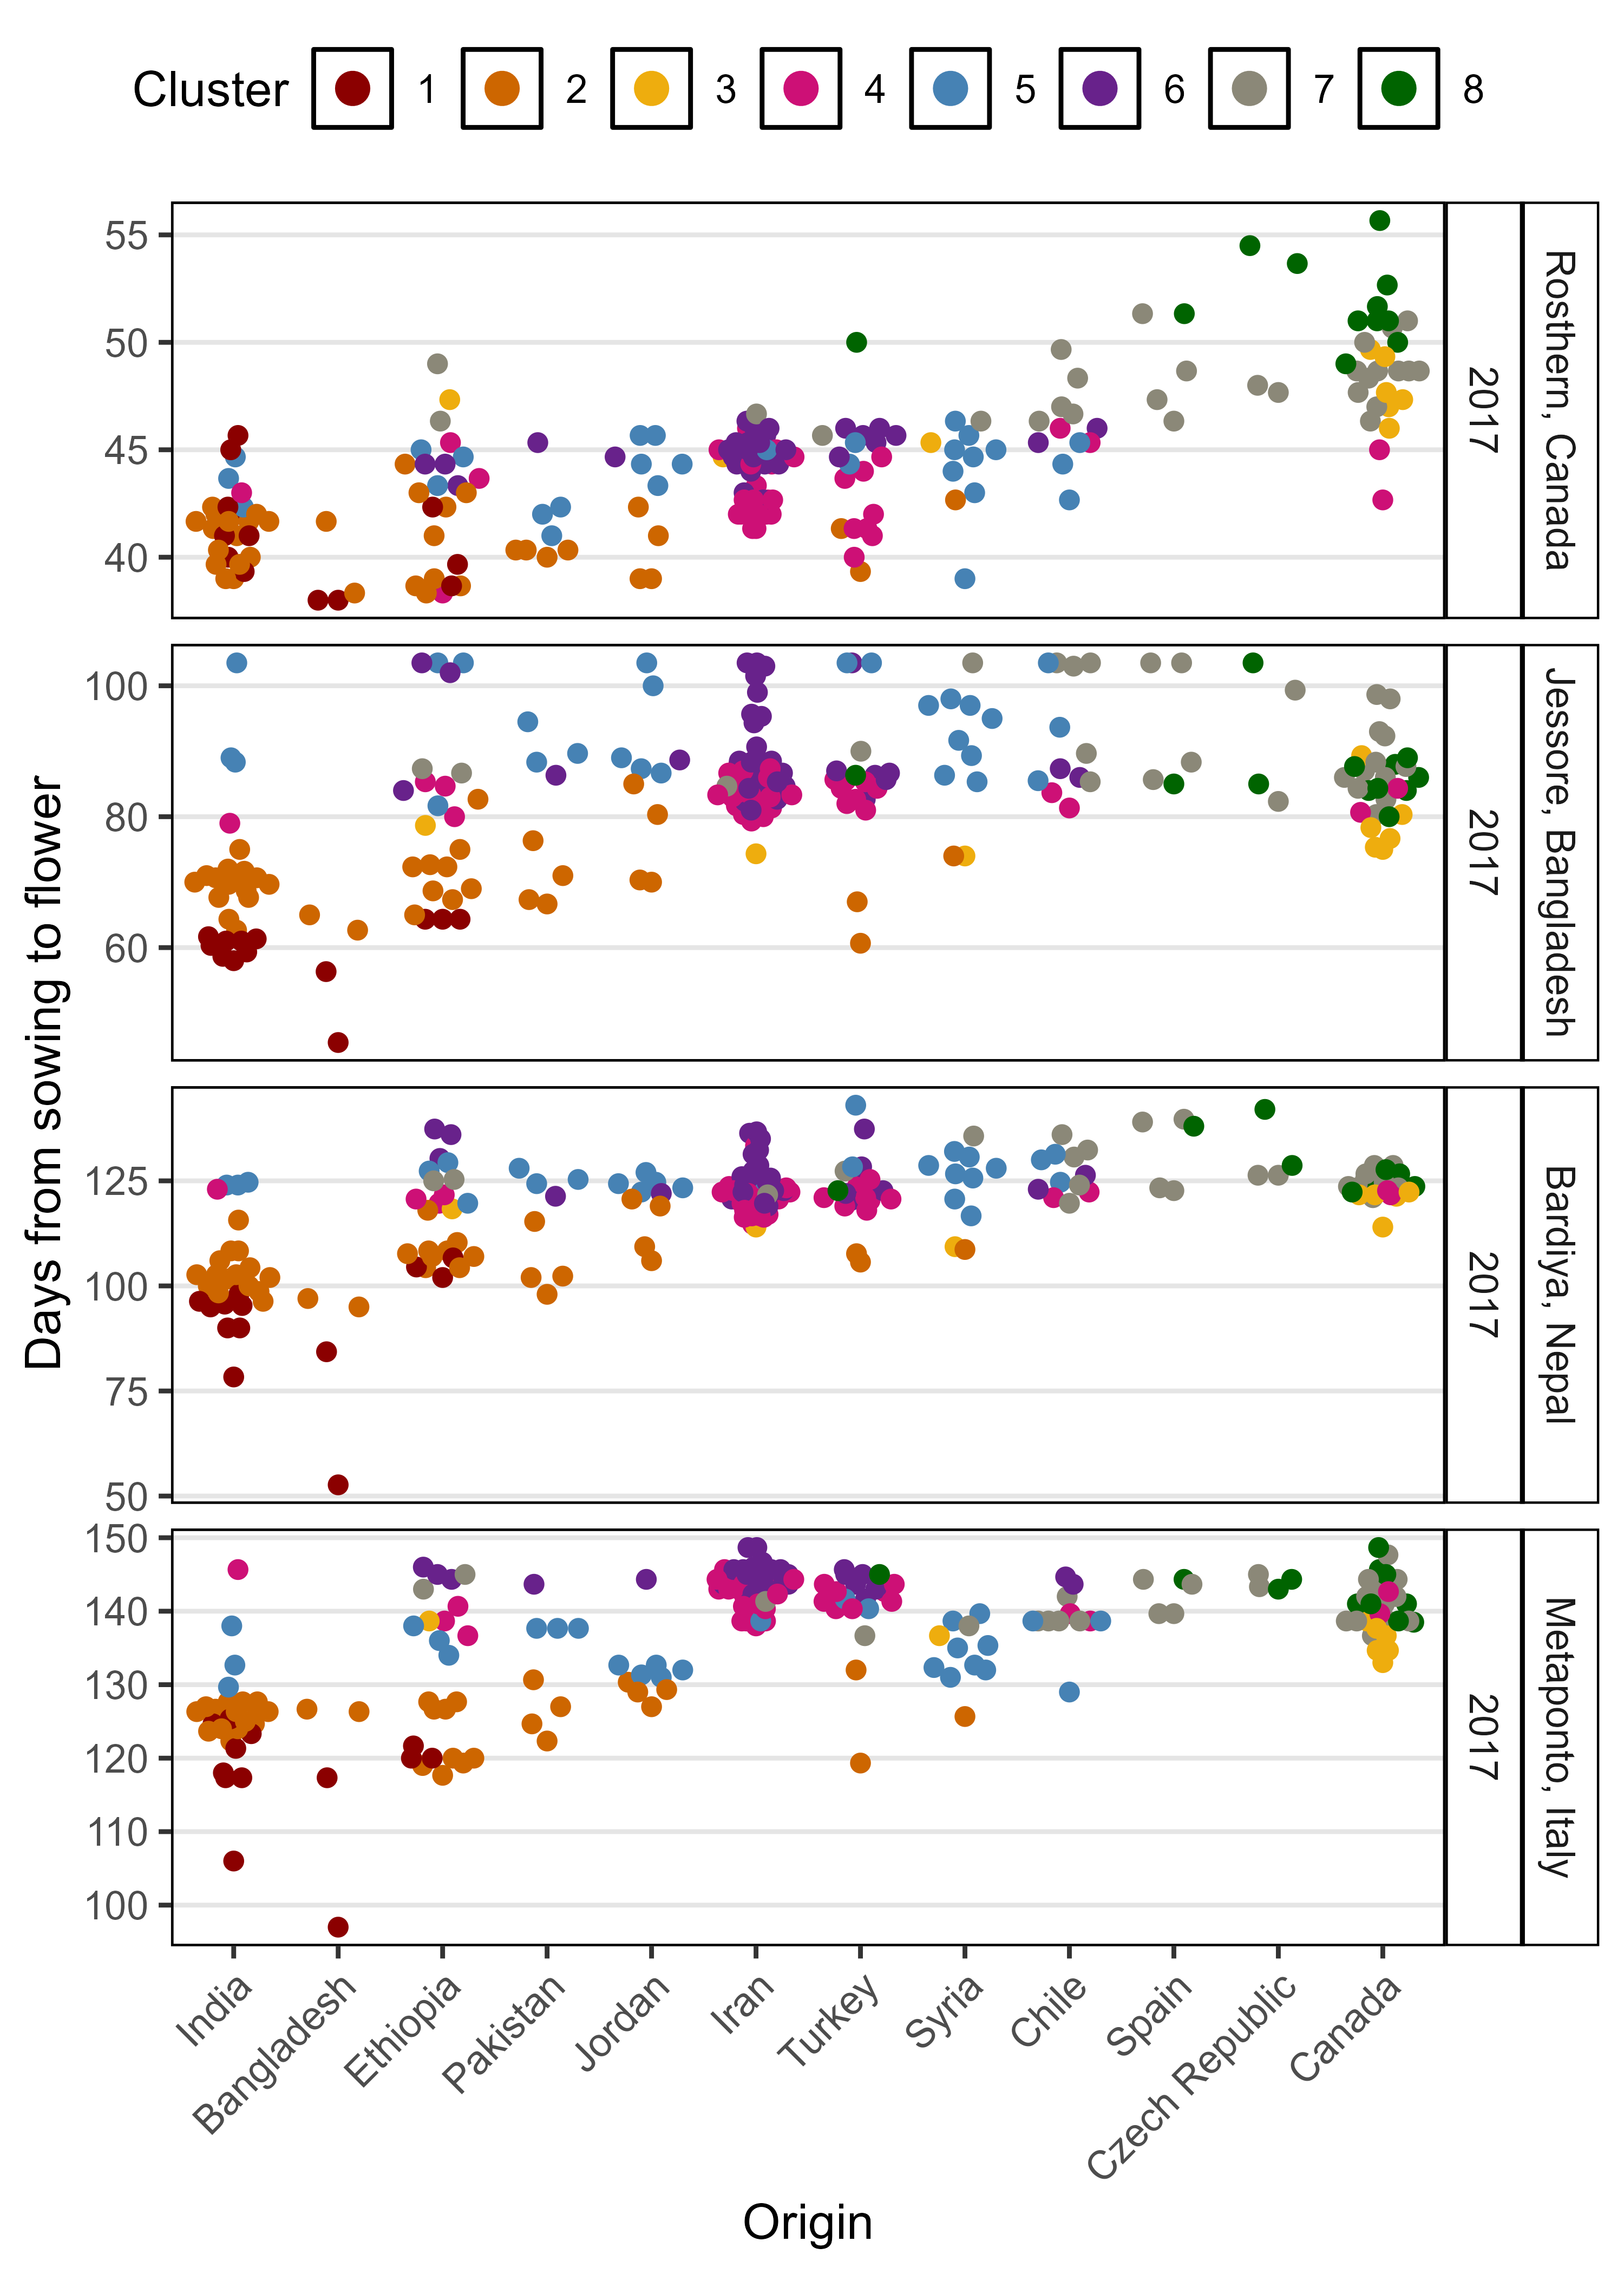
\includegraphics{Additional/Additional_Figure_07.png}

\begin{Shaded}
\begin{Highlighting}[]
\CommentTok{# Prep data}
\NormalTok{x1 <-}\StringTok{ }\KeywordTok{read.csv}\NormalTok{(}\StringTok{"data/data_pca_results.csv"}\NormalTok{) }\OperatorTok\StringTok{ }\KeywordTok{mutate}\NormalTok{(}\DataTypeTok{Cluster =} \KeywordTok{factor}\NormalTok{(Cluster))}
\NormalTok{yy <-}\StringTok{ }\KeywordTok{c}\NormalTok{(}\StringTok{"India"}\NormalTok{, }\StringTok{"Bangladesh"}\NormalTok{, }\StringTok{"Ethiopia"}\NormalTok{, }\StringTok{"Pakistan"}\NormalTok{, }\StringTok{"Jordan"}\NormalTok{,}
        \StringTok{"Iran"}\NormalTok{, }\StringTok{"Turkey"}\NormalTok{, }\StringTok{"Syria"}\NormalTok{, }\StringTok{"Chile"}\NormalTok{, }\StringTok{"Spain"}\NormalTok{, }\StringTok{"Czech Republic"}\NormalTok{, }\StringTok{"Canada"}\NormalTok{ )}
\NormalTok{xx <-}\StringTok{ }\NormalTok{dd }\OperatorTok\StringTok{ }\KeywordTok{left_join}\NormalTok{(ldp, }\DataTypeTok{by =} \StringTok{"Entry"}\NormalTok{) }\OperatorTok
\StringTok{  }\KeywordTok{filter}\NormalTok{(ExptShort }\OperatorTok\StringTok{ }\KeywordTok{c}\NormalTok{(}\StringTok{"Ro17"}\NormalTok{, }\StringTok{"Ba17"}\NormalTok{, }\StringTok{"Ne17"}\NormalTok{, }\StringTok{"It17"}\NormalTok{), Origin }\OperatorTok{!=}\StringTok{ "Unknown"}\NormalTok{) }\OperatorTok\StringTok{ }
\StringTok{  }\KeywordTok{left_join}\NormalTok{(}\KeywordTok{select}\NormalTok{(x1, Entry, Cluster), }\DataTypeTok{by =} \StringTok{"Entry"}\NormalTok{) }\OperatorTok
\StringTok{  }\KeywordTok{mutate}\NormalTok{(}\DataTypeTok{Origin =} \KeywordTok{factor}\NormalTok{(Origin, }\DataTypeTok{levels =} \KeywordTok{unique}\NormalTok{(Origin)[}\KeywordTok{rev}\NormalTok{(}\KeywordTok{order}\NormalTok{(}\KeywordTok{unique}\NormalTok{(Origin)))])) }\OperatorTok
\StringTok{  }\KeywordTok{filter}\NormalTok{(Origin }\OperatorTok\StringTok{ }\NormalTok{yy) }\OperatorTok
\StringTok{  }\KeywordTok{mutate}\NormalTok{(}\DataTypeTok{Origin =} \KeywordTok{factor}\NormalTok{(Origin, }\DataTypeTok{levels =}\NormalTok{ yy))}
\CommentTok{# Plot}
\NormalTok{mp <-}\StringTok{ }\KeywordTok{ggplot}\NormalTok{(xx, }\KeywordTok{aes}\NormalTok{(}\DataTypeTok{y =}\NormalTok{ DTF2, }\DataTypeTok{x =}\NormalTok{ Origin)) }\OperatorTok{+}\StringTok{ }
\StringTok{  }\KeywordTok{geom_quasirandom}\NormalTok{(}\KeywordTok{aes}\NormalTok{(}\DataTypeTok{color =}\NormalTok{ Cluster)) }\OperatorTok{+}\StringTok{ }
\StringTok{  }\KeywordTok{facet_grid}\NormalTok{(Location}\OperatorTok{+}\NormalTok{Year }\OperatorTok{~}\StringTok{ }\NormalTok{., }\DataTypeTok{scales =} \StringTok{"free_y"}\NormalTok{) }\OperatorTok{+}
\StringTok{  }\KeywordTok{scale_color_manual}\NormalTok{(}\DataTypeTok{values =}\NormalTok{ colors) }\OperatorTok{+}\StringTok{ }
\StringTok{  }\NormalTok{theme_AGL }\OperatorTok{+}\StringTok{ }
\StringTok{  }\KeywordTok{theme}\NormalTok{(}\DataTypeTok{legend.position =} \StringTok{"top"}\NormalTok{,}
        \DataTypeTok{panel.grid.major.x =} \KeywordTok{element_blank}\NormalTok{(),}
        \DataTypeTok{axis.text.x =} \KeywordTok{element_text}\NormalTok{(}\DataTypeTok{angle =} \DecValTok{90}\NormalTok{, }\DataTypeTok{hjust =} \DecValTok{1}\NormalTok{, }\DataTypeTok{vjust =} \FloatTok{0.5}\NormalTok{)) }\OperatorTok{+}
\StringTok{  }\KeywordTok{guides}\NormalTok{(}\DataTypeTok{colour =} \KeywordTok{guide_legend}\NormalTok{(}\DataTypeTok{nrow =} \DecValTok{1}\NormalTok{, }\DataTypeTok{override.aes =} \KeywordTok{list}\NormalTok{(}\DataTypeTok{size =} \DecValTok{3}\NormalTok{))) }\OperatorTok{+}
\StringTok{  }\KeywordTok{labs}\NormalTok{(}\DataTypeTok{y =} \StringTok{"Days from sowing to flower"}\NormalTok{)}
\KeywordTok{ggsave}\NormalTok{(}\StringTok{"Additional/Additional_Figure_07.png"}\NormalTok{, mp, }\DataTypeTok{width =} \DecValTok{5}\NormalTok{, }\DataTypeTok{height =} \DecValTok{7}\NormalTok{, }\DataTypeTok{dpi =} \DecValTok{600}\NormalTok{)}
\end{Highlighting}
\end{Shaded}

\hypertarget{additional-figure-8-cluster-origins}{%
\subsection{Additional Figure 8 Cluster
Origins}\label{additional-figure-8-cluster-origins}}

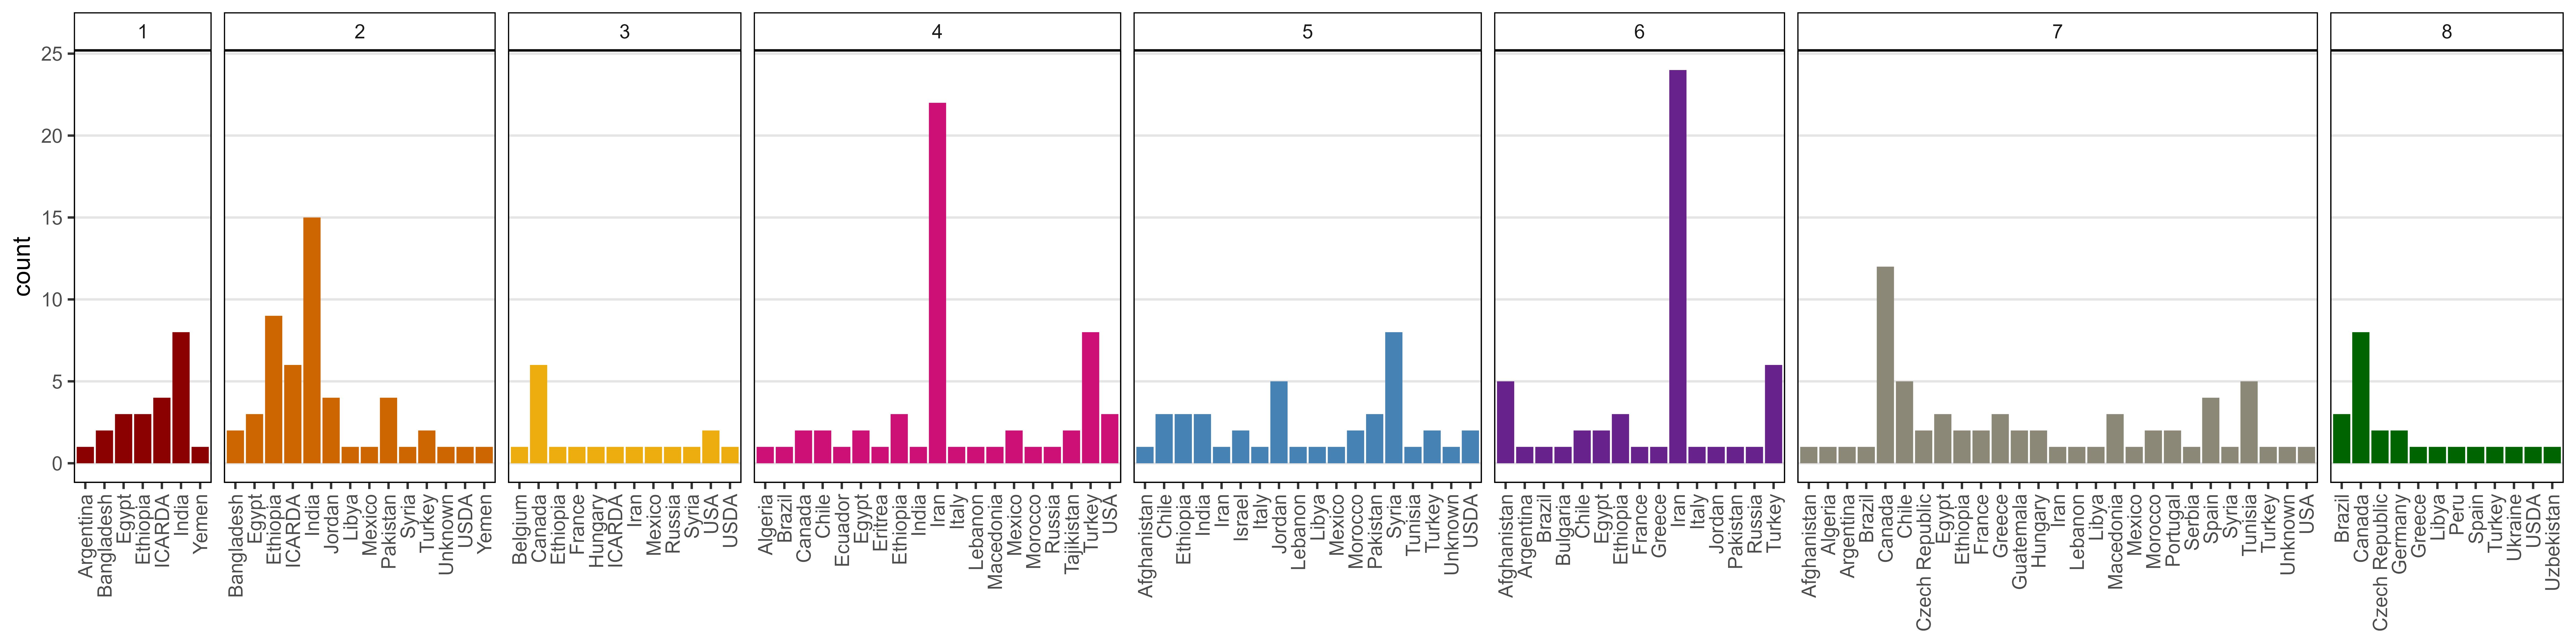
\includegraphics{Additional/Additional_Figure_08.png}

\begin{Shaded}
\begin{Highlighting}[]
\CommentTok{# Prep data}
\NormalTok{pca <-}\StringTok{ }\KeywordTok{read.csv}\NormalTok{(}\StringTok{"data/data_pca_results.csv"}\NormalTok{) }\OperatorTok\StringTok{ }\KeywordTok{mutate}\NormalTok{(}\DataTypeTok{Cluster =} \KeywordTok{factor}\NormalTok{(Cluster))}
\NormalTok{xx <-}\StringTok{ }\NormalTok{ldp }\OperatorTok\StringTok{ }\KeywordTok{left_join}\NormalTok{(}\KeywordTok{select}\NormalTok{(pca, Entry, Cluster), }\DataTypeTok{by =} \StringTok{"Entry"}\NormalTok{) }\OperatorTok
\StringTok{  }\KeywordTok{mutate}\NormalTok{(}\DataTypeTok{test1 =} \KeywordTok{factor}\NormalTok{(}\KeywordTok{paste}\NormalTok{(Origin, Cluster)))}
\NormalTok{x1 <-}\StringTok{ }\NormalTok{xx }\OperatorTok\StringTok{ }\KeywordTok{filter}\NormalTok{(Origin }\OperatorTok{!=}\StringTok{ "ICARDA"}\NormalTok{) }\OperatorTok\StringTok{ }
\StringTok{  }\KeywordTok{group_by}\NormalTok{(Origin, Cluster) }\OperatorTok\StringTok{ }\KeywordTok{summarise}\NormalTok{(}\DataTypeTok{Count =} \KeywordTok{n}\NormalTok{()) }\OperatorTok\StringTok{ }
\StringTok{  }\KeywordTok{spread}\NormalTok{(Cluster, Count) }\OperatorTok
\StringTok{  }\KeywordTok{left_join}\NormalTok{(}\KeywordTok{select}\NormalTok{(ct, }\DataTypeTok{Origin=}\NormalTok{Country, Lat, Lon), }\DataTypeTok{by =} \StringTok{"Origin"}\NormalTok{) }\OperatorTok\StringTok{ }
\StringTok{  }\KeywordTok{ungroup}\NormalTok{() }\OperatorTok\StringTok{ }\KeywordTok{as.data.frame}\NormalTok{()}
\NormalTok{x1[}\KeywordTok{is.na}\NormalTok{(x1)] <-}\StringTok{ }\DecValTok{0} 
\CommentTok{# Plot}
\NormalTok{mp <-}\StringTok{ }\KeywordTok{ggplot}\NormalTok{(xx, }\KeywordTok{aes}\NormalTok{(}\DataTypeTok{x =}\NormalTok{ Origin, }\DataTypeTok{fill =}\NormalTok{ Cluster)) }\OperatorTok{+}\StringTok{ }
\StringTok{  }\KeywordTok{geom_bar}\NormalTok{(}\DataTypeTok{stat =} \StringTok{"count"}\NormalTok{) }\OperatorTok{+}\StringTok{ }
\StringTok{  }\KeywordTok{facet_grid}\NormalTok{(. }\OperatorTok{~}\StringTok{ }\NormalTok{Cluster, }\DataTypeTok{scales =} \StringTok{"free"}\NormalTok{, }\DataTypeTok{space =} \StringTok{"free"}\NormalTok{) }\OperatorTok{+}\StringTok{ }
\StringTok{  }\KeywordTok{scale_fill_manual}\NormalTok{(}\DataTypeTok{values =}\NormalTok{ colors) }\OperatorTok{+}
\StringTok{  }\NormalTok{theme_AGL }\OperatorTok{+}
\StringTok{  }\KeywordTok{theme}\NormalTok{(}\DataTypeTok{legend.position =} \StringTok{"none"}\NormalTok{,}
        \DataTypeTok{panel.grid.major.x =} \KeywordTok{element_blank}\NormalTok{(),}
        \DataTypeTok{axis.text.x =} \KeywordTok{element_text}\NormalTok{(}\DataTypeTok{angle =} \DecValTok{90}\NormalTok{, }\DataTypeTok{hjust =} \DecValTok{1}\NormalTok{, }\DataTypeTok{vjust =} \FloatTok{0.5}\NormalTok{)) }\OperatorTok{+}
\StringTok{  }\KeywordTok{labs}\NormalTok{(}\DataTypeTok{x =} \OtherTok{NULL}\NormalTok{)}
\KeywordTok{ggsave}\NormalTok{(}\StringTok{"Additional/Additional_Figure_08.png"}\NormalTok{, }\DataTypeTok{width =} \DecValTok{16}\NormalTok{, }\DataTypeTok{height =} \DecValTok{4}\NormalTok{, }\DataTypeTok{dpi =} \DecValTok{600}\NormalTok{)}
\end{Highlighting}
\end{Shaded}

\hypertarget{additional-figure-9-ldp-origins-by-cluster}{%
\subsection{Additional Figure 9 LDP Origins By
Cluster}\label{additional-figure-9-ldp-origins-by-cluster}}

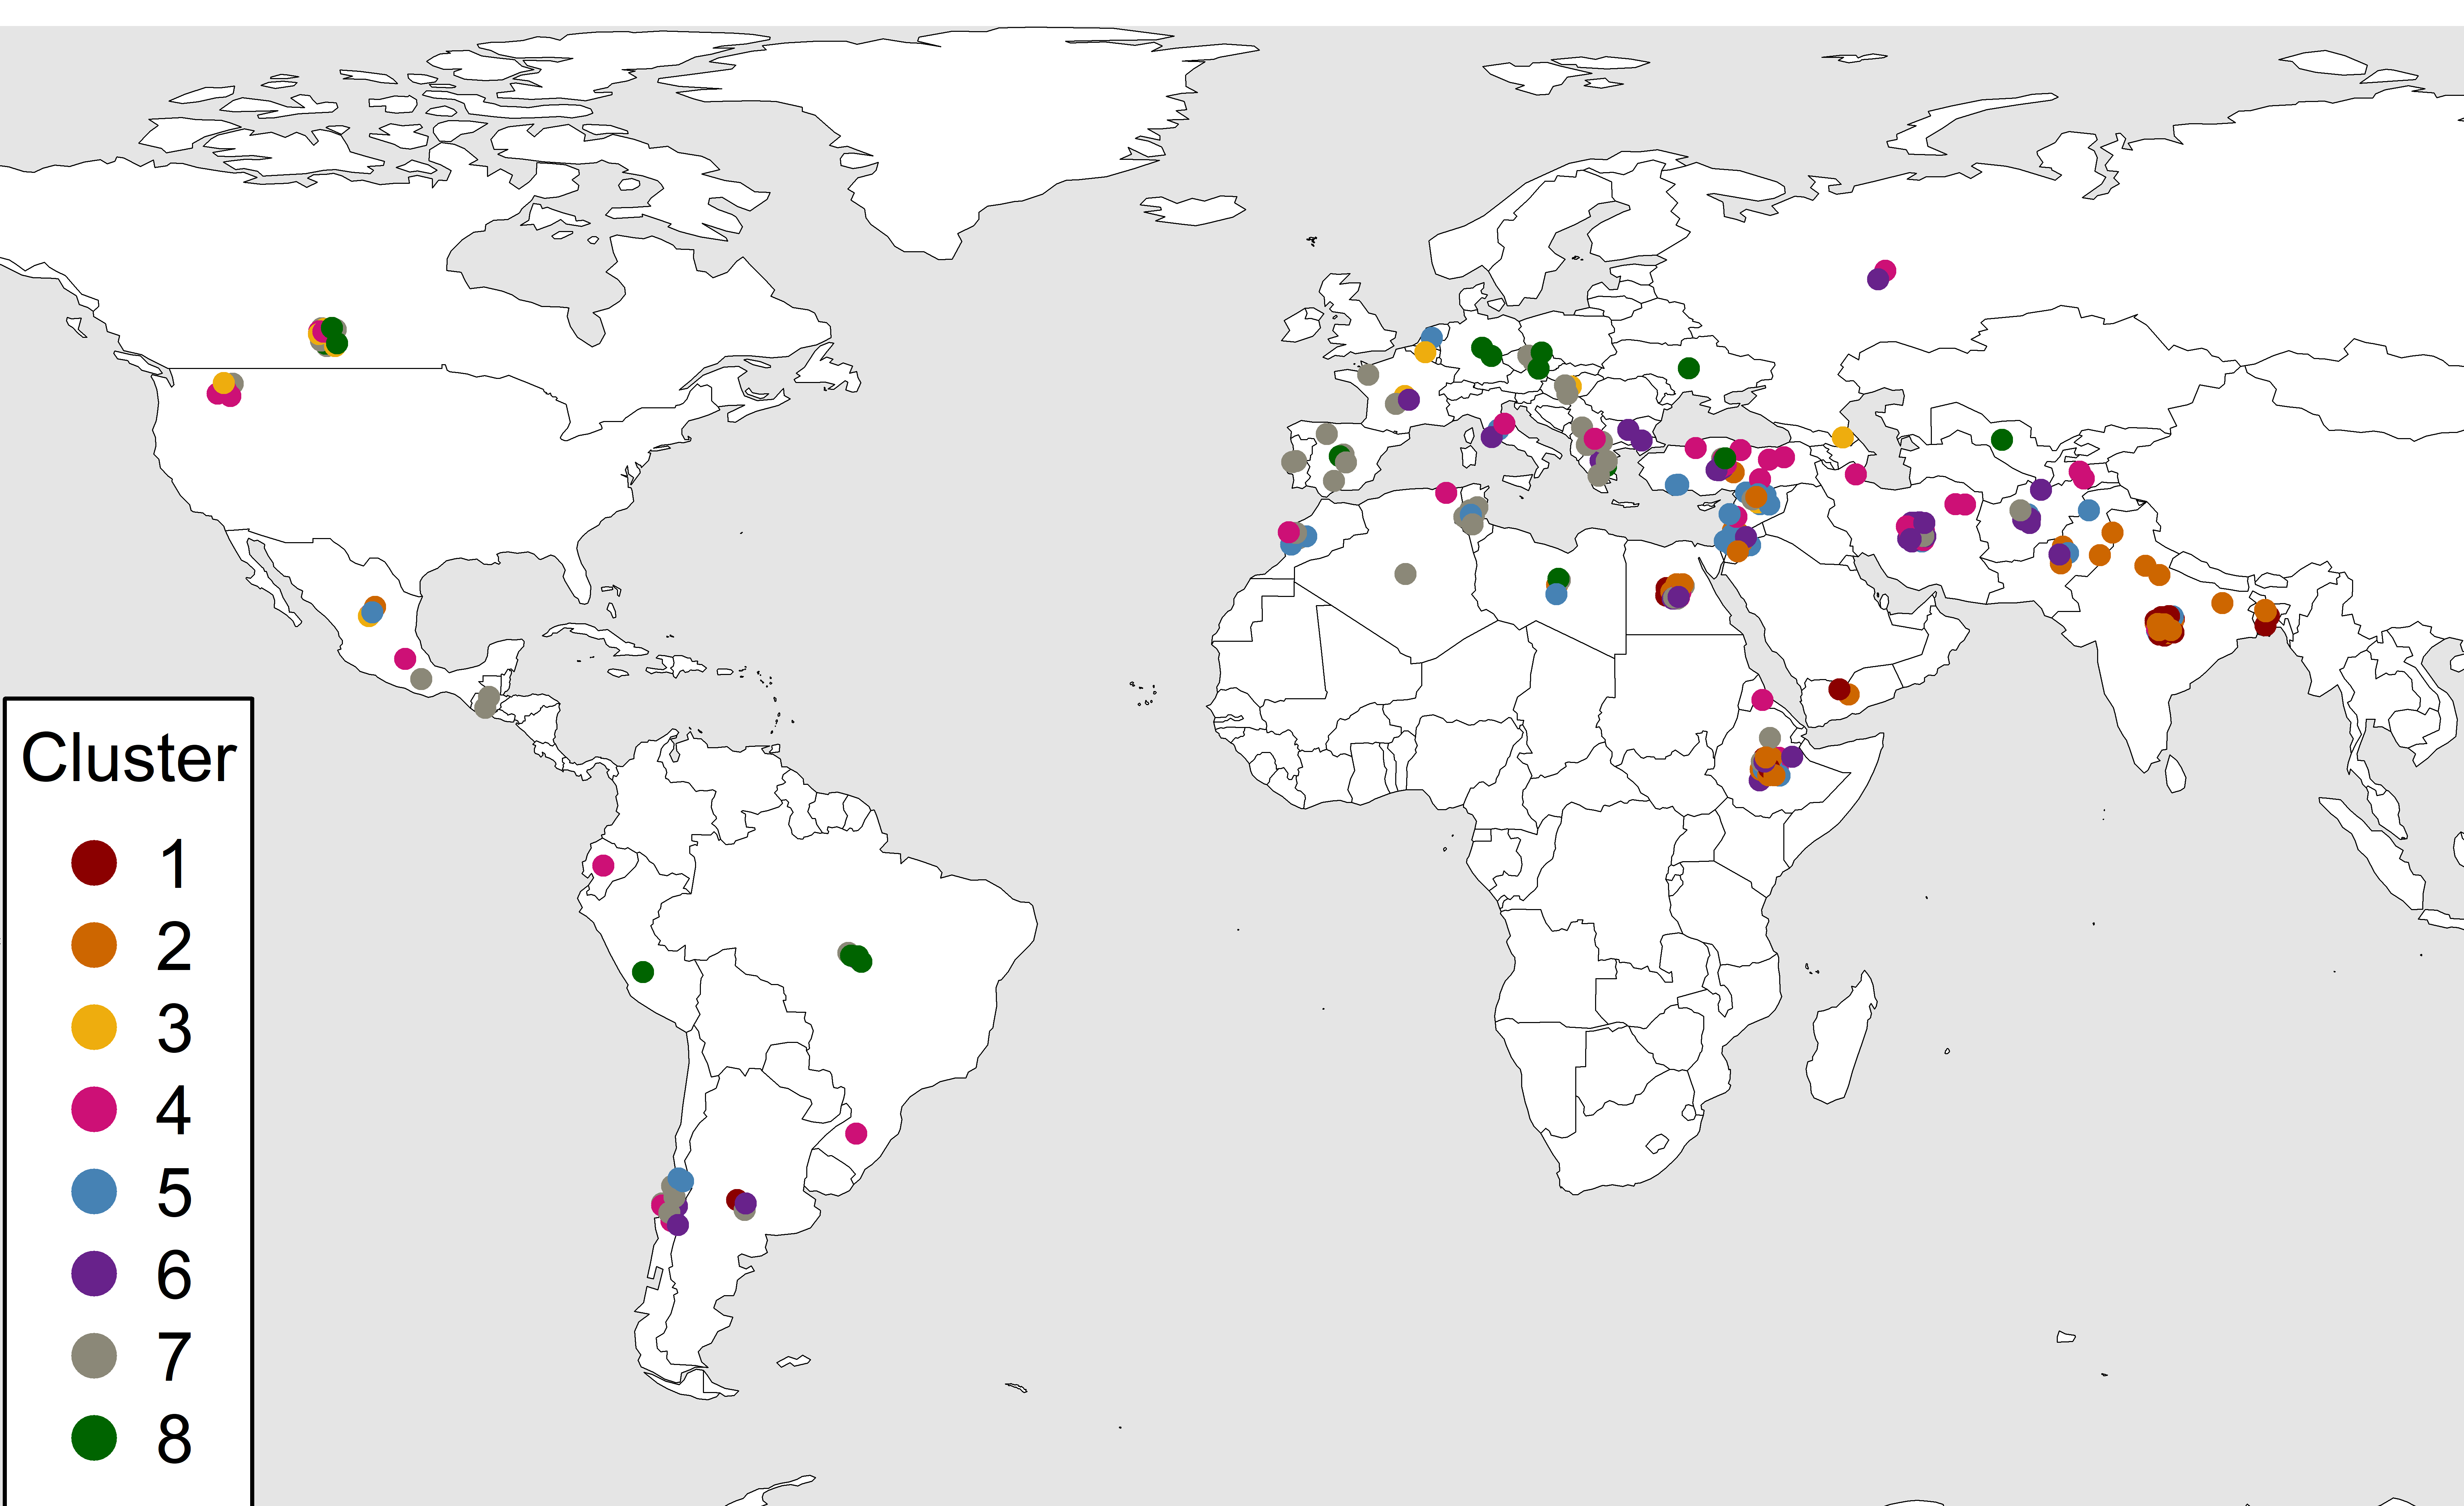
\includegraphics{Additional/Additional_Figure_09.png}

\begin{Shaded}
\begin{Highlighting}[]
\CommentTok{# Prep data}
\NormalTok{x1 <-}\StringTok{ }\KeywordTok{read.csv}\NormalTok{(}\StringTok{"data/data_pca_results.csv"}\NormalTok{) }\OperatorTok\StringTok{ }\KeywordTok{mutate}\NormalTok{(}\DataTypeTok{Cluster =} \KeywordTok{factor}\NormalTok{(Cluster))}
\NormalTok{xx <-}\StringTok{ }\NormalTok{ldp }\OperatorTok\StringTok{ }\KeywordTok{select}\NormalTok{(Entry, Name, Lat, Lon) }\OperatorTok\StringTok{ }\KeywordTok{left_join}\NormalTok{(x1, }\DataTypeTok{by =} \StringTok{"Entry"}\NormalTok{) }\OperatorTok
\StringTok{  }\KeywordTok{left_join}\NormalTok{(}\KeywordTok{select}\NormalTok{(ct, }\DataTypeTok{Origin=}\NormalTok{Country, }\DataTypeTok{cLat=}\NormalTok{Lat, }\DataTypeTok{cLon=}\NormalTok{Lon), }\DataTypeTok{by =} \StringTok{"Origin"}\NormalTok{) }\OperatorTok
\StringTok{  }\KeywordTok{mutate}\NormalTok{(}\DataTypeTok{Lat =} \KeywordTok{ifelse}\NormalTok{(}\KeywordTok{is.na}\NormalTok{(Lat), cLat, Lat),}
         \DataTypeTok{Lon =} \KeywordTok{ifelse}\NormalTok{(}\KeywordTok{is.na}\NormalTok{(Lon), cLon, Lon),}
         \DataTypeTok{Lat =} \KeywordTok{ifelse}\NormalTok{(}\KeywordTok{duplicated}\NormalTok{(Lat), }\KeywordTok{jitter}\NormalTok{(Lat, }\DecValTok{1}\NormalTok{, }\DecValTok{1}\NormalTok{), Lat),}
         \DataTypeTok{Lon =} \KeywordTok{ifelse}\NormalTok{(}\KeywordTok{duplicated}\NormalTok{(Lon), }\KeywordTok{jitter}\NormalTok{(Lon, }\DecValTok{1}\NormalTok{, }\DecValTok{1}\NormalTok{), Lon), }\DataTypeTok{Size =} \DecValTok{1}\NormalTok{)}
\CommentTok{# Plot}
\KeywordTok{invisible}\NormalTok{(}\KeywordTok{png}\NormalTok{(}\StringTok{"Additional/Additional_Figure_09.png"}\NormalTok{, }
              \DataTypeTok{width =} \DecValTok{7200}\NormalTok{, }\DataTypeTok{height =} \DecValTok{4400}\NormalTok{, }\DataTypeTok{res =} \DecValTok{600}\NormalTok{)) }\CommentTok{#res = 150}
\KeywordTok{par}\NormalTok{(}\DataTypeTok{mai =} \KeywordTok{c}\NormalTok{(}\DecValTok{0}\NormalTok{,}\DecValTok{0}\NormalTok{,}\DecValTok{0}\NormalTok{,}\DecValTok{0}\NormalTok{), }\DataTypeTok{xaxs =} \StringTok{"i"}\NormalTok{, }\DataTypeTok{yaxs =} \StringTok{"i"}\NormalTok{)}
\KeywordTok{mapBubbles}\NormalTok{(}\DataTypeTok{dF =}\NormalTok{ xx, }\DataTypeTok{nameX =} \StringTok{"Lon"}\NormalTok{, }\DataTypeTok{nameY =} \StringTok{"Lat"}\NormalTok{, }\DataTypeTok{nameZColour =} \StringTok{"Cluster"}\NormalTok{,}
           \DataTypeTok{nameZSize =} \StringTok{"Size"}\NormalTok{, }\DataTypeTok{symbolSize =} \FloatTok{0.5}\NormalTok{, }\DataTypeTok{pch =} \DecValTok{20}\NormalTok{, }\DataTypeTok{addLegend =}\NormalTok{ F,}
           \DataTypeTok{colourPalette =}\NormalTok{ colors[}\DecValTok{1}\OperatorTok{:}\DecValTok{8}\NormalTok{], }\DataTypeTok{addColourLegend =}\NormalTok{ F,}
           \DataTypeTok{xlim =} \KeywordTok{c}\NormalTok{(}\OperatorTok{-}\DecValTok{140}\NormalTok{,}\DecValTok{110}\NormalTok{), }\DataTypeTok{ylim =} \KeywordTok{c}\NormalTok{(}\DecValTok{0}\NormalTok{,}\DecValTok{20}\NormalTok{), }
           \DataTypeTok{oceanCol =} \StringTok{"grey90"}\NormalTok{, }\DataTypeTok{landCol =} \StringTok{"white"}\NormalTok{, }\DataTypeTok{borderCol =} \StringTok{"black"}\NormalTok{)}
\KeywordTok{legend}\NormalTok{(}\OperatorTok{-}\FloatTok{139.5}\NormalTok{, }\FloatTok{15.5}\NormalTok{, }\DataTypeTok{title =} \StringTok{"Cluster"}\NormalTok{, }\DataTypeTok{legend =} \DecValTok{1}\OperatorTok{:}\DecValTok{8}\NormalTok{, }\DataTypeTok{col =}\NormalTok{ colors,}
       \DataTypeTok{pch =} \DecValTok{16}\NormalTok{, }\DataTypeTok{cex =} \DecValTok{2}\NormalTok{, }\DataTypeTok{pt.cex =} \DecValTok{3}\NormalTok{, }\DataTypeTok{box.lwd =} \DecValTok{2}\NormalTok{)}
\KeywordTok{invisible}\NormalTok{(}\KeywordTok{dev.off}\NormalTok{())}
\end{Highlighting}
\end{Shaded}

\hypertarget{modeling-dtf}{%
\section{Modeling DTF}\label{modeling-dtf}}

\hypertarget{additional-figures---entry-regressions}{%
\subsection{Additional Figures - Entry
Regressions}\label{additional-figures---entry-regressions}}

\begin{Shaded}
\begin{Highlighting}[]
\NormalTok{myfills <-}\StringTok{ }\KeywordTok{alpha}\NormalTok{(}\KeywordTok{c}\NormalTok{(}\StringTok{"darkgreen"}\NormalTok{, }\StringTok{"darkorange3"}\NormalTok{, }\StringTok{"darkblue"}\NormalTok{), }\FloatTok{0.5}\NormalTok{)}
\NormalTok{mymin <-}\StringTok{ }\KeywordTok{min}\NormalTok{(rr}\OperatorTok{$}\NormalTok{RDTF, }\DataTypeTok{na.rm =}\NormalTok{ T); mymax <-}\StringTok{ }\KeywordTok{max}\NormalTok{(rr}\OperatorTok{$}\NormalTok{RDTF, }\DataTypeTok{na.rm =}\NormalTok{ T)}
\NormalTok{mp <-}\StringTok{ }\KeywordTok{list}\NormalTok{()}
\ControlFlowTok{for}\NormalTok{(i }\ControlFlowTok{in} \DecValTok{1}\OperatorTok{:}\DecValTok{324}\NormalTok{) \{}
\NormalTok{  xx <-}\StringTok{ }\NormalTok{rr }\OperatorTok\StringTok{ }\KeywordTok{filter}\NormalTok{(Entry }\OperatorTok{==}\StringTok{ }\NormalTok{i) }\OperatorTok
\StringTok{    }\KeywordTok{left_join}\NormalTok{(}\KeywordTok{select}\NormalTok{(ff, Expt, MacroEnv, T_mean, P_mean), }\DataTypeTok{by =} \StringTok{"Expt"}\NormalTok{) }\OperatorTok
\StringTok{    }\KeywordTok{mutate}\NormalTok{(}\DataTypeTok{myfill =}\NormalTok{ MacroEnv)}
\NormalTok{  x1 <-}\StringTok{ }\NormalTok{xx }\OperatorTok\StringTok{ }\KeywordTok{filter}\NormalTok{(MacroEnv }\OperatorTok{!=}\StringTok{ "South Asia"}\NormalTok{)}
\NormalTok{  x2 <-}\StringTok{ }\NormalTok{xx }\OperatorTok\StringTok{ }\KeywordTok{filter}\NormalTok{(MacroEnv }\OperatorTok{!=}\StringTok{ "Temperate"}\NormalTok{)}
\NormalTok{  x3 <-}\StringTok{ }\NormalTok{xx }\OperatorTok\StringTok{ }\KeywordTok{filter}\NormalTok{(MacroEnv }\OperatorTok{!=}\StringTok{ "Mediterranean"}\NormalTok{)}
\NormalTok{  figlab <-}\StringTok{ }\KeywordTok{paste}\NormalTok{(}\StringTok{"Entry"}\NormalTok{, }\KeywordTok{str_pad}\NormalTok{(i, }\DecValTok{3}\NormalTok{, }\StringTok{"left"}\NormalTok{, }\StringTok{"0"}\NormalTok{), }\StringTok{"|"}\NormalTok{, }\KeywordTok{unique}\NormalTok{(xx}\OperatorTok{$}\NormalTok{Name))}
  \CommentTok{# Plot (a) 1/f = a + bT}
\NormalTok{  mp1 <-}\StringTok{ }\KeywordTok{ggplot}\NormalTok{(xx, }\KeywordTok{aes}\NormalTok{(}\DataTypeTok{x =}\NormalTok{ T_mean, }\DataTypeTok{y =}\NormalTok{ RDTF)) }\OperatorTok{+}
\StringTok{    }\KeywordTok{geom_point}\NormalTok{(}\KeywordTok{aes}\NormalTok{(}\DataTypeTok{shape =}\NormalTok{ MacroEnv, }\DataTypeTok{color =}\NormalTok{ MacroEnv)) }\OperatorTok{+}
\StringTok{    }\KeywordTok{geom_smooth}\NormalTok{(}\DataTypeTok{data =}\NormalTok{ x1, }\DataTypeTok{method =} \StringTok{"lm"}\NormalTok{, }\DataTypeTok{se =}\NormalTok{ F, }\DataTypeTok{color =} \StringTok{"black"}\NormalTok{, }\DataTypeTok{lty =} \DecValTok{3}\NormalTok{) }\OperatorTok{+}
\StringTok{    }\KeywordTok{geom_smooth}\NormalTok{(}\DataTypeTok{data =}\NormalTok{ x2, }\DataTypeTok{method =} \StringTok{"lm"}\NormalTok{, }\DataTypeTok{se =}\NormalTok{ F, }\DataTypeTok{color =} \StringTok{"black"}\NormalTok{) }\OperatorTok{+}
\StringTok{    }\KeywordTok{scale_y_continuous}\NormalTok{(}\DataTypeTok{sec.axis =} \KeywordTok{dup_axis}\NormalTok{(}\OperatorTok{~}\StringTok{ }\DecValTok{1}\OperatorTok{/}\NormalTok{., }\DataTypeTok{name =} \OtherTok{NULL}\NormalTok{, }\DataTypeTok{breaks =} \KeywordTok{c}\NormalTok{(}\DecValTok{35}\NormalTok{,}\DecValTok{50}\NormalTok{,}\DecValTok{100}\NormalTok{,}\DecValTok{150}\NormalTok{)),}
                       \DataTypeTok{trans =} \StringTok{"reverse"}\NormalTok{, }\DataTypeTok{breaks =} \KeywordTok{c}\NormalTok{(}\FloatTok{0.01}\NormalTok{,}\FloatTok{0.02}\NormalTok{,}\FloatTok{0.03}\NormalTok{), }
                       \DataTypeTok{limits =} \KeywordTok{c}\NormalTok{(mymax, mymin)) }\OperatorTok{+}
\StringTok{    }\KeywordTok{scale_x_continuous}\NormalTok{(}\DataTypeTok{breaks =} \KeywordTok{c}\NormalTok{(}\DecValTok{11}\NormalTok{,}\DecValTok{13}\NormalTok{,}\DecValTok{15}\NormalTok{,}\DecValTok{17}\NormalTok{,}\DecValTok{19}\NormalTok{,}\DecValTok{21}\NormalTok{)) }\OperatorTok{+}
\StringTok{    }\KeywordTok{scale_shape_manual}\NormalTok{(}\DataTypeTok{name =} \StringTok{"Macro-environment"}\NormalTok{, }\DataTypeTok{values =} \KeywordTok{c}\NormalTok{(}\DecValTok{16}\NormalTok{,}\DecValTok{15}\NormalTok{,}\DecValTok{17}\NormalTok{)) }\OperatorTok{+}
\StringTok{    }\KeywordTok{scale_color_manual}\NormalTok{(}\DataTypeTok{name =} \StringTok{"Macro-environment"}\NormalTok{, }\DataTypeTok{values =}\NormalTok{ myfills) }\OperatorTok{+}
\StringTok{    }\NormalTok{theme_AGL }\OperatorTok{+}\StringTok{ }
\StringTok{    }\KeywordTok{labs}\NormalTok{(}\DataTypeTok{title =}\NormalTok{ figlab, }\DataTypeTok{y =} \StringTok{"1 / DTF"}\NormalTok{, }
         \DataTypeTok{x =} \KeywordTok{expression}\NormalTok{(}\KeywordTok{paste}\NormalTok{(}\StringTok{"Temperature ("}\NormalTok{, degree, }\StringTok{"C)"}\NormalTok{, }\DataTypeTok{sep =} \StringTok{""}\NormalTok{)))}
  \CommentTok{# Plot (b) 1/f = a + cP}
\NormalTok{  mp2 <-}\StringTok{ }\KeywordTok{ggplot}\NormalTok{(xx, }\KeywordTok{aes}\NormalTok{(}\DataTypeTok{x =}\NormalTok{ P_mean, }\DataTypeTok{y =}\NormalTok{ RDTF)) }\OperatorTok{+}
\StringTok{    }\KeywordTok{geom_point}\NormalTok{(}\KeywordTok{aes}\NormalTok{(}\DataTypeTok{shape =}\NormalTok{ MacroEnv, }\DataTypeTok{color =}\NormalTok{ MacroEnv)) }\OperatorTok{+}
\StringTok{    }\KeywordTok{geom_smooth}\NormalTok{(}\DataTypeTok{data =}\NormalTok{ x1, }\DataTypeTok{method =} \StringTok{"lm"}\NormalTok{, }\DataTypeTok{se =}\NormalTok{ F, }\DataTypeTok{color =} \StringTok{"black"}\NormalTok{, }\DataTypeTok{lty =} \DecValTok{3}\NormalTok{) }\OperatorTok{+}
\StringTok{    }\KeywordTok{geom_smooth}\NormalTok{(}\DataTypeTok{data =}\NormalTok{ x3, }\DataTypeTok{method =} \StringTok{"lm"}\NormalTok{, }\DataTypeTok{se =}\NormalTok{ F, }\DataTypeTok{color =} \StringTok{"black"}\NormalTok{) }\OperatorTok{+}
\StringTok{    }\KeywordTok{scale_y_continuous}\NormalTok{(}\DataTypeTok{sec.axis =} \KeywordTok{dup_axis}\NormalTok{(}\OperatorTok{~}\StringTok{ }\DecValTok{1}\OperatorTok{/}\NormalTok{., }\DataTypeTok{name=}\StringTok{"DTF"}\NormalTok{, }\DataTypeTok{breaks =} \KeywordTok{c}\NormalTok{(}\DecValTok{35}\NormalTok{,}\DecValTok{50}\NormalTok{,}\DecValTok{100}\NormalTok{,}\DecValTok{150}\NormalTok{)),}
                       \DataTypeTok{trans =} \StringTok{"reverse"}\NormalTok{, }\DataTypeTok{breaks =} \KeywordTok{c}\NormalTok{(}\FloatTok{0.01}\NormalTok{,}\FloatTok{0.02}\NormalTok{,}\FloatTok{0.03}\NormalTok{), }
                       \DataTypeTok{limits =} \KeywordTok{c}\NormalTok{(mymax, mymin)) }\OperatorTok{+}
\StringTok{    }\KeywordTok{scale_x_continuous}\NormalTok{(}\DataTypeTok{breaks =} \KeywordTok{c}\NormalTok{(}\DecValTok{11}\NormalTok{,}\DecValTok{12}\NormalTok{,}\DecValTok{13}\NormalTok{,}\DecValTok{14}\NormalTok{,}\DecValTok{15}\NormalTok{,}\DecValTok{16}\NormalTok{)) }\OperatorTok{+}
\StringTok{    }\KeywordTok{scale_shape_manual}\NormalTok{(}\DataTypeTok{name =} \StringTok{"Macro-environment"}\NormalTok{, }\DataTypeTok{values =} \KeywordTok{c}\NormalTok{(}\DecValTok{16}\NormalTok{,}\DecValTok{15}\NormalTok{,}\DecValTok{17}\NormalTok{)) }\OperatorTok{+}
\StringTok{    }\KeywordTok{scale_color_manual}\NormalTok{(}\DataTypeTok{name =} \StringTok{"Macro-environment"}\NormalTok{, }\DataTypeTok{values =}\NormalTok{ myfills) }\OperatorTok{+}
\StringTok{    }\NormalTok{theme_AGL }\OperatorTok{+}
\StringTok{    }\KeywordTok{labs}\NormalTok{(}\DataTypeTok{title =} \StringTok{""}\NormalTok{, }\DataTypeTok{y =} \OtherTok{NULL}\NormalTok{,}\DataTypeTok{x =} \StringTok{"Photoperiod (hours)"}\NormalTok{)}
  \CommentTok{#}
\NormalTok{  mp[[i]] <-}\StringTok{ }\KeywordTok{ggarrange}\NormalTok{(mp1, mp2, }\DataTypeTok{ncol =} \DecValTok{2}\NormalTok{, }\DataTypeTok{common.legend =}\NormalTok{ T, }\DataTypeTok{legend =} \StringTok{"bottom"}\NormalTok{) }
  \KeywordTok{ggsave}\NormalTok{(}\KeywordTok{paste0}\NormalTok{(}\StringTok{"Additional/Entry_TP/TP_Entry_"}\NormalTok{, }\KeywordTok{str_pad}\NormalTok{(i, }\DecValTok{3}\NormalTok{, }\DataTypeTok{pad =} \StringTok{"0"}\NormalTok{), }\StringTok{".png"}\NormalTok{), }
\NormalTok{         mp[[i]], }\DataTypeTok{width =} \DecValTok{8}\NormalTok{, }\DataTypeTok{height =} \DecValTok{4}\NormalTok{, }\DataTypeTok{dpi =} \DecValTok{600}\NormalTok{)}
\NormalTok{\}}
\KeywordTok{pdf}\NormalTok{(}\StringTok{"Additional/pdf_TP.pdf"}\NormalTok{, }\DataTypeTok{width =} \DecValTok{8}\NormalTok{, }\DataTypeTok{height =} \DecValTok{4}\NormalTok{)}
\ControlFlowTok{for}\NormalTok{(i }\ControlFlowTok{in} \DecValTok{1}\OperatorTok{:}\DecValTok{324}\NormalTok{) \{ }\KeywordTok{print}\NormalTok{(mp[[i]]) \}}
\KeywordTok{dev.off}\NormalTok{() }\CommentTok{#dev.set(dev.next())}
\end{Highlighting}
\end{Shaded}

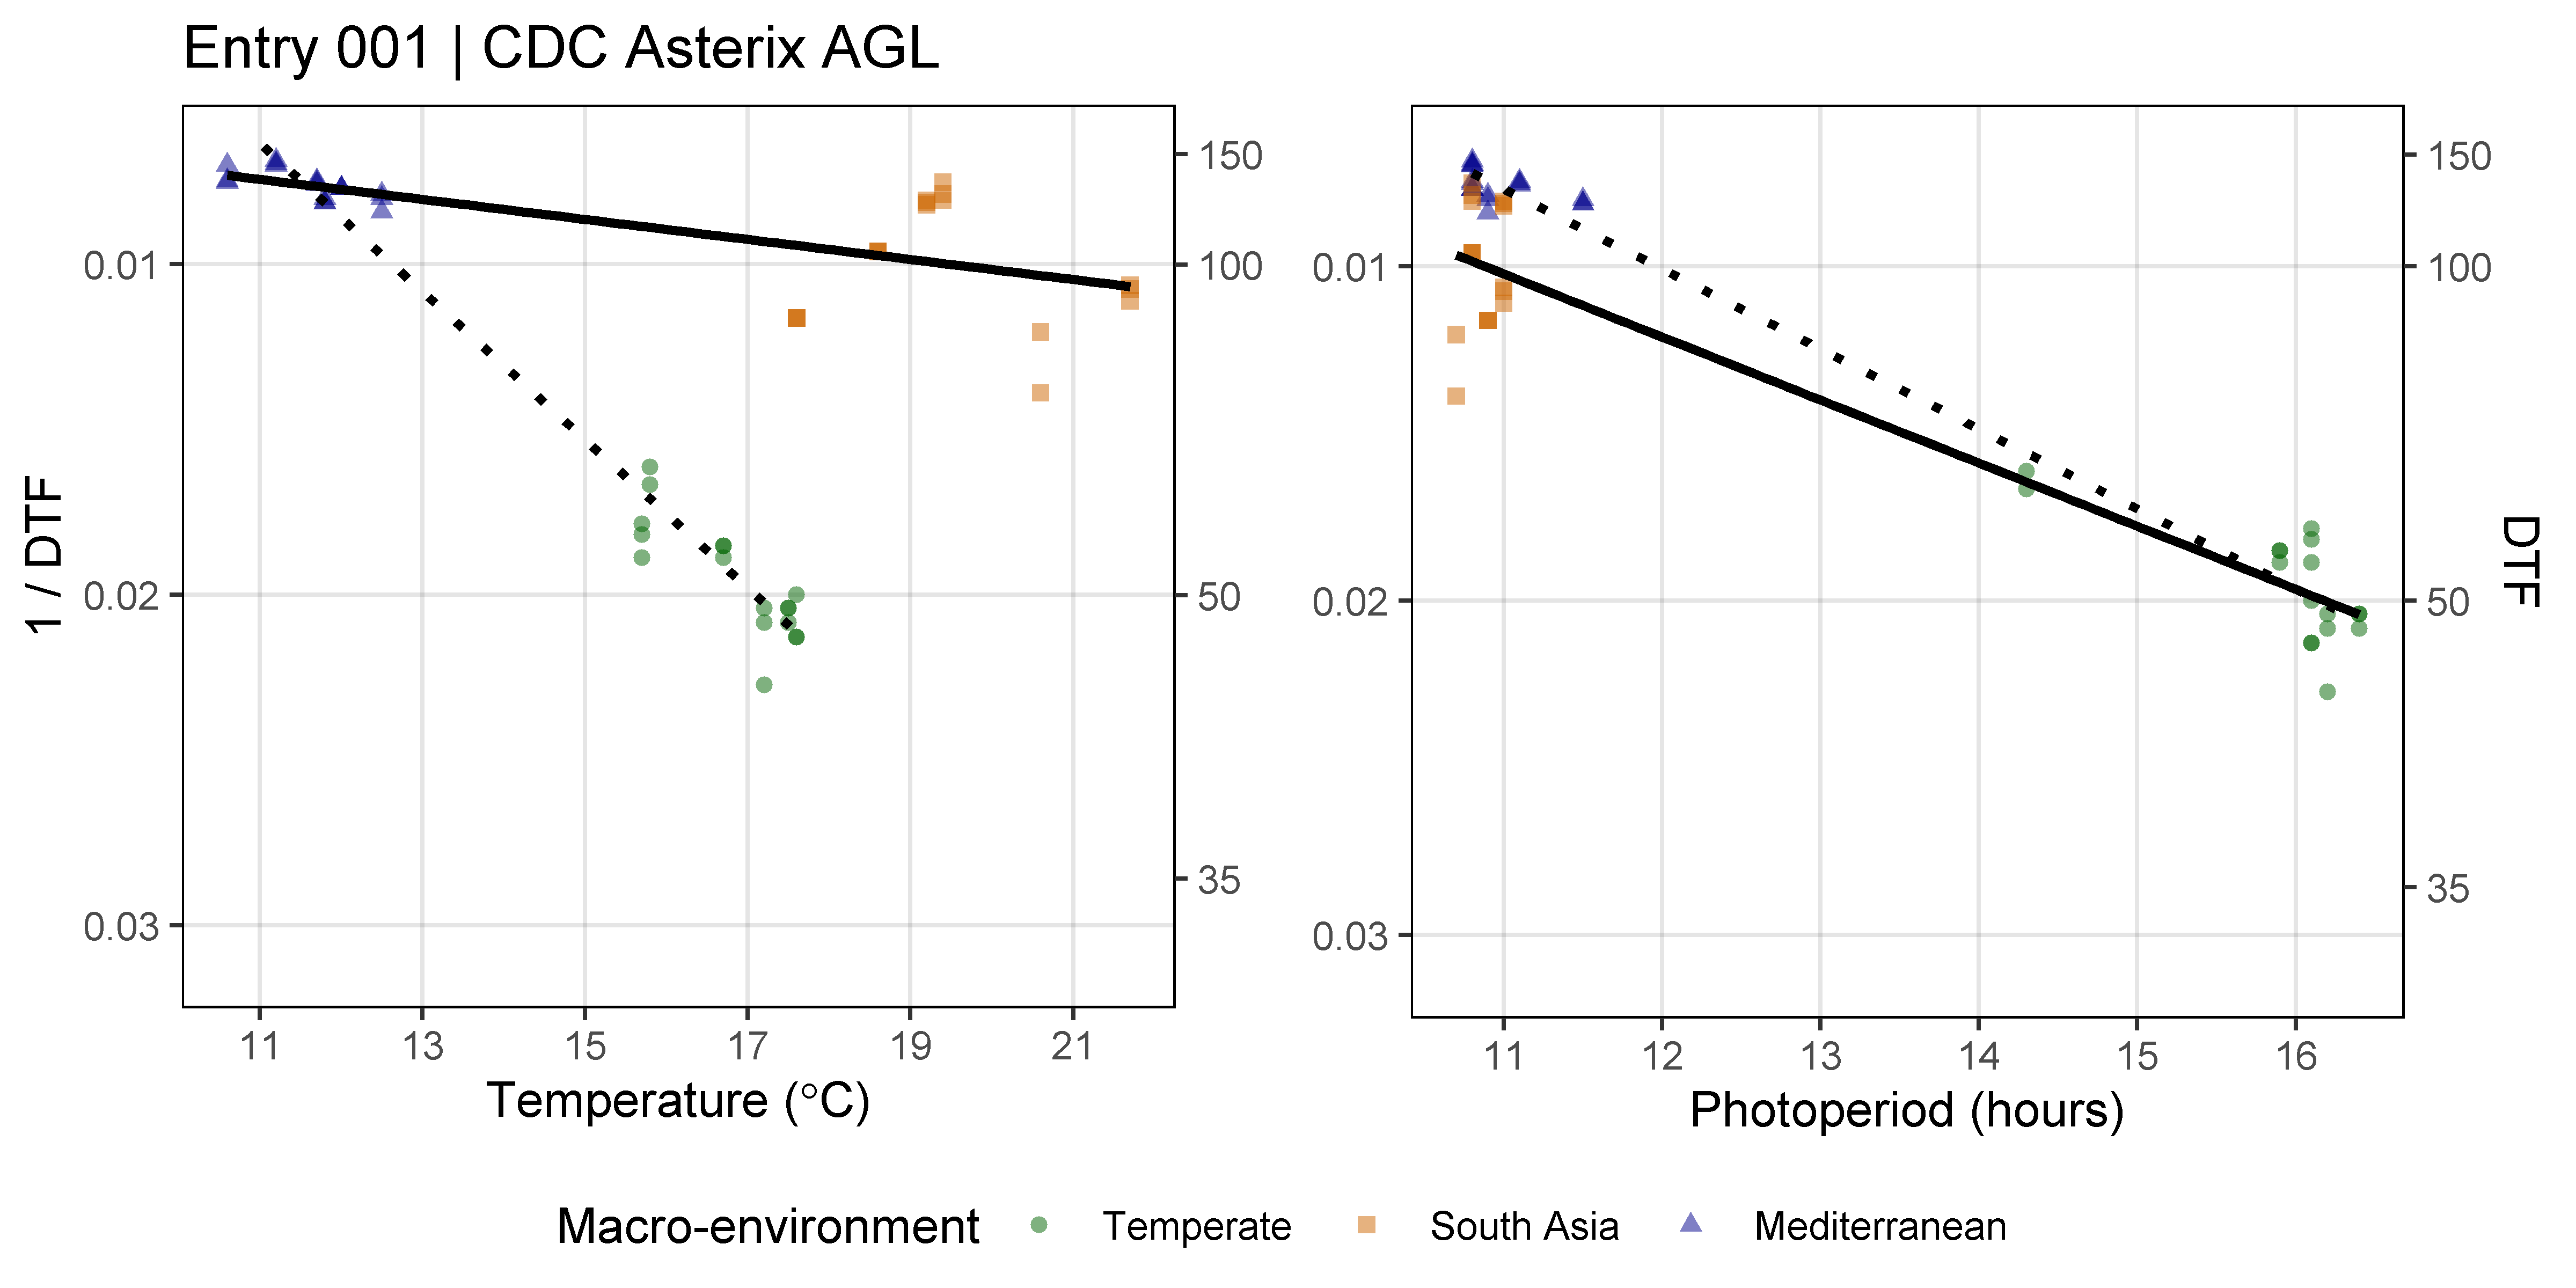
\includegraphics{Additional/Entry_TP/TP_Entry_001.png}

\hypertarget{photothermal-plane}{%
\subsection{PhotoThermal Plane}\label{photothermal-plane}}

\begin{Shaded}
\begin{Highlighting}[]
\CommentTok{# Prep data}
\NormalTok{xx <-}\StringTok{ }\NormalTok{rr }\OperatorTok\StringTok{ }\KeywordTok{filter}\NormalTok{(}\OperatorTok{!}\KeywordTok{is.na}\NormalTok{(RDTF)) }\OperatorTok
\StringTok{  }\KeywordTok{left_join}\NormalTok{(}\KeywordTok{select}\NormalTok{(ff, Expt, T_mean, P_mean, MacroEnv), }\DataTypeTok{by =} \StringTok{"Expt"}\NormalTok{)}
\CommentTok{# Create plotting function}
\NormalTok{gg_PTplane <-}\StringTok{ }\ControlFlowTok{function}\NormalTok{(x, i) \{}
\NormalTok{  x1 <-}\StringTok{ }\NormalTok{x }\OperatorTok\StringTok{ }\KeywordTok{filter}\NormalTok{(Entry }\OperatorTok{==}\StringTok{ }\NormalTok{i)}
\NormalTok{  x <-}\StringTok{ }\NormalTok{x1}\OperatorTok{$}\NormalTok{T_mean}
\NormalTok{  y <-}\StringTok{ }\NormalTok{x1}\OperatorTok{$}\NormalTok{P_mean}
\NormalTok{  z <-}\StringTok{ }\NormalTok{x1}\OperatorTok{$}\NormalTok{RDTF}
\NormalTok{  fit <-}\StringTok{ }\KeywordTok{lm}\NormalTok{(z }\OperatorTok{~}\StringTok{ }\NormalTok{x }\OperatorTok{+}\StringTok{ }\NormalTok{y)}
  \CommentTok{# Create PhotoThermal plane}
\NormalTok{  fitp <-}\StringTok{ }\KeywordTok{predict}\NormalTok{(fit)}
\NormalTok{  grid.lines <-}\StringTok{ }\DecValTok{12}
\NormalTok{  x.p <-}\StringTok{ }\KeywordTok{seq}\NormalTok{(}\KeywordTok{min}\NormalTok{(x), }\KeywordTok{max}\NormalTok{(x), }\DataTypeTok{length.out =}\NormalTok{ grid.lines)}
\NormalTok{  y.p <-}\StringTok{ }\KeywordTok{seq}\NormalTok{(}\KeywordTok{min}\NormalTok{(y), }\KeywordTok{max}\NormalTok{(y), }\DataTypeTok{length.out =}\NormalTok{ grid.lines)}
\NormalTok{  xy <-}\StringTok{ }\KeywordTok{expand.grid}\NormalTok{(}\DataTypeTok{x =}\NormalTok{ x.p, }\DataTypeTok{y =}\NormalTok{ y.p)}
\NormalTok{  z.p <-}\StringTok{ }\KeywordTok{matrix}\NormalTok{(}\KeywordTok{predict}\NormalTok{(fit, }\DataTypeTok{newdata =}\NormalTok{ xy), }\DataTypeTok{nrow =}\NormalTok{ grid.lines, }\DataTypeTok{ncol =}\NormalTok{ grid.lines)}
\NormalTok{  pchs <-}\StringTok{ }\NormalTok{plyr}\OperatorTok{::}\KeywordTok{mapvalues}\NormalTok{(x1}\OperatorTok{$}\NormalTok{Expt, names_Expt, }\KeywordTok{c}\NormalTok{(}\KeywordTok{rep}\NormalTok{(}\DecValTok{16}\NormalTok{,}\DecValTok{6}\NormalTok{),}\KeywordTok{rep}\NormalTok{(}\DecValTok{15}\NormalTok{,}\DecValTok{6}\NormalTok{),}\KeywordTok{rep}\NormalTok{(}\DecValTok{17}\NormalTok{,}\DecValTok{6}\NormalTok{))) }\OperatorTok
\StringTok{    }\KeywordTok{as.character}\NormalTok{() }\OperatorTok\StringTok{ }\KeywordTok{as.numeric}\NormalTok{()}
  \CommentTok{# Plot with regression plane}
  \KeywordTok{par}\NormalTok{(}\DataTypeTok{mar=}\KeywordTok{c}\NormalTok{(}\FloatTok{1.5}\NormalTok{, }\FloatTok{2.5}\NormalTok{, }\FloatTok{1.5}\NormalTok{, }\FloatTok{0.5}\NormalTok{))}
  \KeywordTok{scatter3D}\NormalTok{(x, y, z, }\DataTypeTok{pch =}\NormalTok{ pchs, }\DataTypeTok{cex =} \DecValTok{2}\NormalTok{, }\DataTypeTok{main =} \KeywordTok{unique}\NormalTok{(x1}\OperatorTok{$}\NormalTok{Name),}
    \DataTypeTok{col =} \KeywordTok{alpha}\NormalTok{(}\KeywordTok{c}\NormalTok{(}\StringTok{"darkgreen"}\NormalTok{, }\StringTok{"darkorange3"}\NormalTok{, }\StringTok{"darkblue"}\NormalTok{),}\FloatTok{0.5}\NormalTok{),}
    \DataTypeTok{colvar =} \KeywordTok{as.numeric}\NormalTok{(x1}\OperatorTok{$}\NormalTok{MacroEnv), }\DataTypeTok{colkey =}\NormalTok{ F, }\DataTypeTok{col.grid =} \StringTok{"gray90"}\NormalTok{, }\DataTypeTok{bty =} \StringTok{"u"}\NormalTok{,}
    \DataTypeTok{theta =} \DecValTok{40}\NormalTok{, }\DataTypeTok{phi =} \DecValTok{25}\NormalTok{, }\DataTypeTok{ticktype =} \StringTok{"detailed"}\NormalTok{, }\DataTypeTok{cex.lab =} \DecValTok{1}\NormalTok{, }\DataTypeTok{cex.axis =} \FloatTok{0.5}\NormalTok{,}
    \DataTypeTok{xlab =} \StringTok{"Temperature"}\NormalTok{, }\DataTypeTok{ylab =} \StringTok{"Photoperiod"}\NormalTok{, }\DataTypeTok{zlab =} \StringTok{"1 / DTF"}\NormalTok{, }\DataTypeTok{zlim =} \KeywordTok{c}\NormalTok{(}\FloatTok{0.005}\NormalTok{,}\FloatTok{0.03}\NormalTok{),}
    \DataTypeTok{surf =} \KeywordTok{list}\NormalTok{(}\DataTypeTok{x =}\NormalTok{ x.p, }\DataTypeTok{y =}\NormalTok{ y.p, }\DataTypeTok{z =}\NormalTok{ z.p, }\DataTypeTok{col =} \StringTok{"black"}\NormalTok{, }\DataTypeTok{facets =} \OtherTok{NA}\NormalTok{, }\DataTypeTok{fit =}\NormalTok{ fitp) )}
\NormalTok{\}}
\CommentTok{# Plot each Entry}
\ControlFlowTok{for}\NormalTok{ (i }\ControlFlowTok{in} \DecValTok{1}\OperatorTok{:}\DecValTok{324}\NormalTok{) \{}
  \KeywordTok{png}\NormalTok{(}\KeywordTok{paste0}\NormalTok{(}\StringTok{"Additional/Entry_3D/3D_Entry_"}\NormalTok{, }\KeywordTok{str_pad}\NormalTok{(i, }\DecValTok{3}\NormalTok{, }\DataTypeTok{pad =} \StringTok{"0"}\NormalTok{), }\StringTok{".png"}\NormalTok{), }
      \DataTypeTok{width =} \DecValTok{1000}\NormalTok{, }\DataTypeTok{height =} \DecValTok{1000}\NormalTok{, }\DataTypeTok{res =} \DecValTok{600}\NormalTok{) }\CommentTok{#res = 200}
  \KeywordTok{gg_PTplane}\NormalTok{(xx, i)}
  \KeywordTok{dev.off}\NormalTok{()}
\NormalTok{\}}
\CommentTok{# Create PDF}
\KeywordTok{pdf}\NormalTok{(}\StringTok{"Additional/pdf_3D.pdf"}\NormalTok{)}
\KeywordTok{par}\NormalTok{(}\DataTypeTok{mar=}\KeywordTok{c}\NormalTok{(}\FloatTok{1.5}\NormalTok{, }\FloatTok{2.5}\NormalTok{, }\FloatTok{1.5}\NormalTok{, }\FloatTok{0.5}\NormalTok{))}
\ControlFlowTok{for}\NormalTok{ (i }\ControlFlowTok{in} \DecValTok{1}\OperatorTok{:}\DecValTok{324}\NormalTok{) \{}
  \KeywordTok{gg_PTplane}\NormalTok{(xx, i)}
\NormalTok{\}}
\KeywordTok{dev.off}\NormalTok{() }\CommentTok{#dev.set(dev.next())}
\CommentTok{#}
\CommentTok{# Plot ILL 5888 & ILL 4400 & Laird}
\NormalTok{xx <-}\StringTok{ }\NormalTok{xx }\OperatorTok\StringTok{ }\KeywordTok{mutate}\NormalTok{(}\DataTypeTok{Name =} \KeywordTok{gsub}\NormalTok{(}\StringTok{" AGL"}\NormalTok{, }\StringTok{""}\NormalTok{, Name))}
\ControlFlowTok{for}\NormalTok{ (i }\ControlFlowTok{in} \KeywordTok{c}\NormalTok{(}\DecValTok{235}\NormalTok{, }\DecValTok{94}\NormalTok{, }\DecValTok{128}\NormalTok{)) \{}
  \KeywordTok{png}\NormalTok{(}\KeywordTok{paste0}\NormalTok{(}\StringTok{"Additional/Temp/3D_Entry_"}\NormalTok{, }\KeywordTok{str_pad}\NormalTok{(i, }\DecValTok{3}\NormalTok{, }\DataTypeTok{pad =} \StringTok{"0"}\NormalTok{), }\StringTok{".png"}\NormalTok{), }
      \DataTypeTok{width =} \DecValTok{1000}\NormalTok{, }\DataTypeTok{height =} \DecValTok{1000}\NormalTok{, }\DataTypeTok{res =} \DecValTok{600}\NormalTok{) }\CommentTok{# res = 200}
  \KeywordTok{gg_PTplane}\NormalTok{(xx, i)}
  \KeywordTok{dev.off}\NormalTok{()}
\NormalTok{\}}
\CommentTok{# Create animation}
\NormalTok{xx <-}\StringTok{ }\KeywordTok{read.csv}\NormalTok{(}\StringTok{"data/model_t+p_coefs.csv"}\NormalTok{) }\OperatorTok\StringTok{ }\KeywordTok{arrange}\NormalTok{(b, c)}
\NormalTok{lf <-}\StringTok{ }\KeywordTok{list.files}\NormalTok{(}\StringTok{"Additional/Entry_3D"}\NormalTok{)[xx}\OperatorTok{$}\NormalTok{Entry]}
\NormalTok{mp <-}\StringTok{ }\KeywordTok{image_read}\NormalTok{(}\KeywordTok{paste0}\NormalTok{(}\StringTok{"Additional/Entry_3D/"}\NormalTok{, lf))}
\NormalTok{animation <-}\StringTok{ }\KeywordTok{image_animate}\NormalTok{(mp, }\DataTypeTok{fps =} \DecValTok{10}\NormalTok{)}
\KeywordTok{image_write}\NormalTok{(animation, }\StringTok{"Additional/Animation_3D.gif"}\NormalTok{)}
\end{Highlighting}
\end{Shaded}

\includegraphics{Additional/Entry_3D/3d_Entry_001.png}

\hypertarget{supplemental-figure-4-regressions}{%
\subsection{Supplemental Figure 4
Regressions}\label{supplemental-figure-4-regressions}}

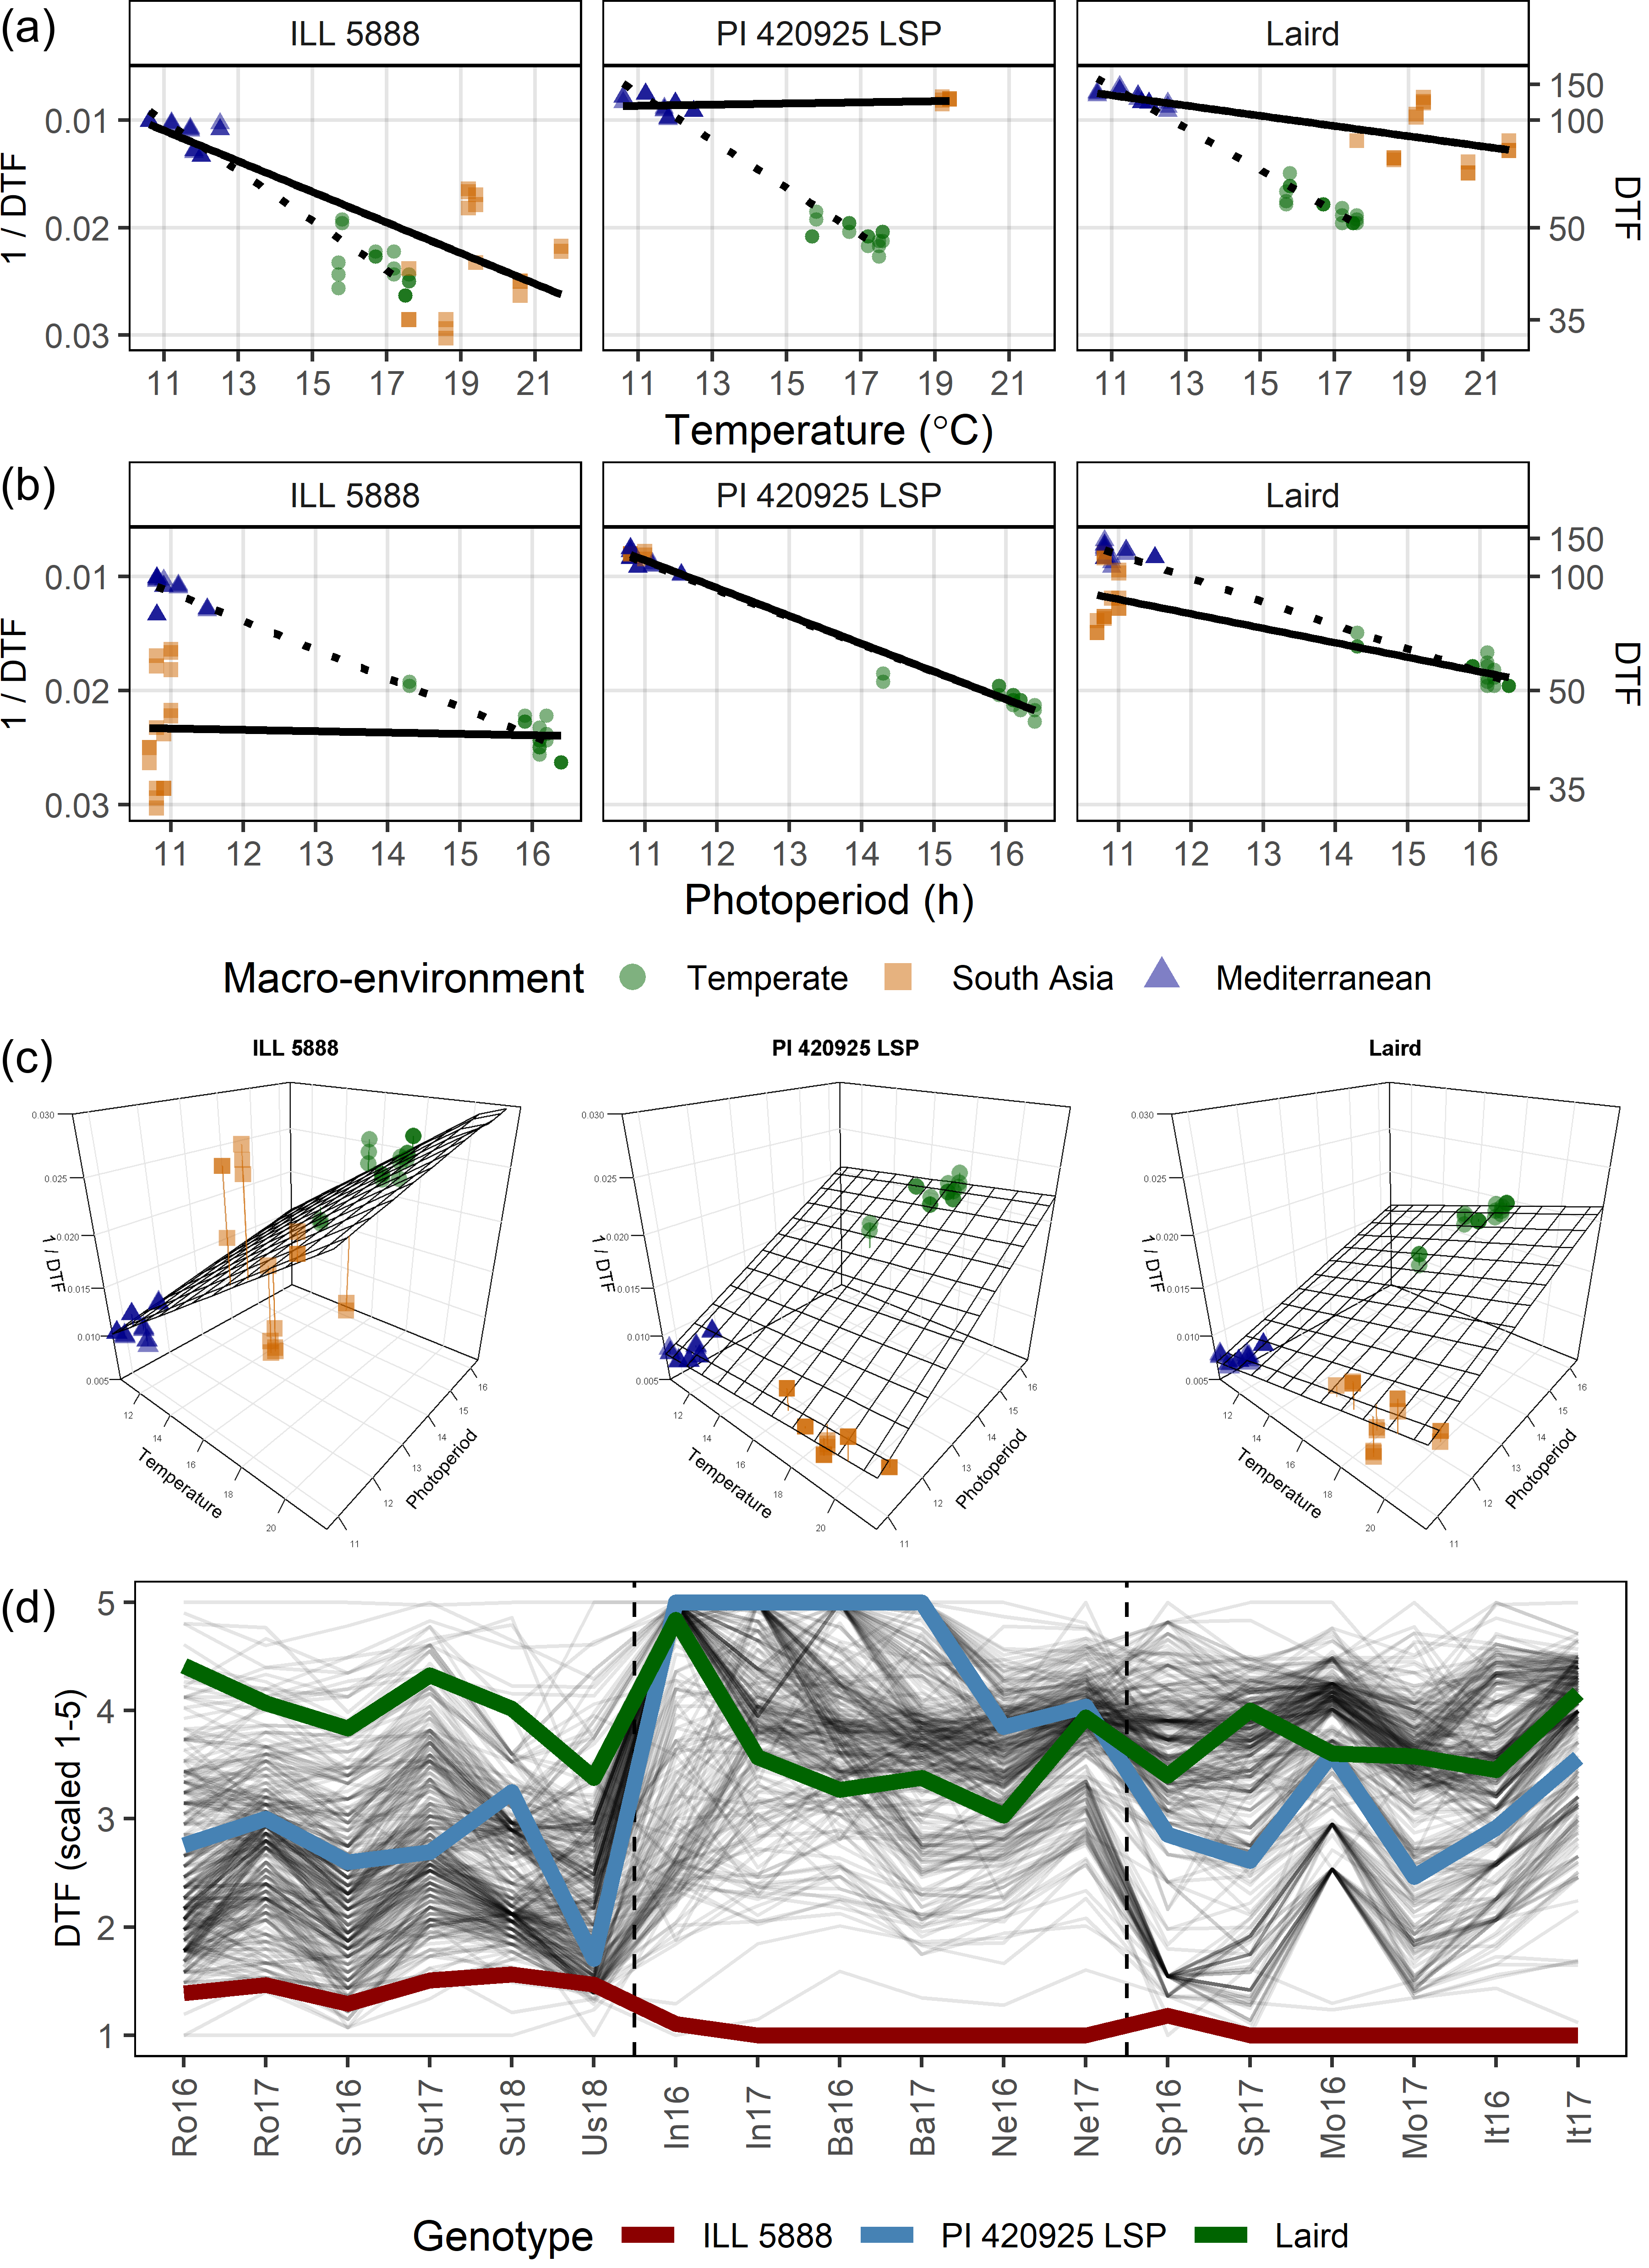
\includegraphics{Supplemental_Figure_04.png}

\begin{Shaded}
\begin{Highlighting}[]
\CommentTok{# Prep data}
\NormalTok{myfills <-}\StringTok{ }\KeywordTok{alpha}\NormalTok{(}\KeywordTok{c}\NormalTok{(}\StringTok{"darkgreen"}\NormalTok{, }\StringTok{"darkorange3"}\NormalTok{, }\StringTok{"darkblue"}\NormalTok{), }\FloatTok{0.5}\NormalTok{)}
\NormalTok{yy <-}\StringTok{ }\KeywordTok{c}\NormalTok{(}\StringTok{"ILL 5888 AGL"}\NormalTok{, }\StringTok{"PI 420925 LSP AGL"}\NormalTok{,  }\StringTok{"Laird AGL"}\NormalTok{)}
\NormalTok{xx <-}\StringTok{ }\NormalTok{rr }\OperatorTok\StringTok{ }\KeywordTok{filter}\NormalTok{(Name }\OperatorTok\StringTok{ }\NormalTok{yy, }\OperatorTok{!}\KeywordTok{is.na}\NormalTok{(DTF)) }\OperatorTok
\StringTok{  }\KeywordTok{left_join}\NormalTok{(}\KeywordTok{select}\NormalTok{(ff, Expt, MacroEnv, T_mean, P_mean), }\DataTypeTok{by =} \StringTok{"Expt"}\NormalTok{) }\OperatorTok
\StringTok{  }\KeywordTok{mutate}\NormalTok{(}\DataTypeTok{Name =} \KeywordTok{gsub}\NormalTok{(}\StringTok{" AGL"}\NormalTok{, }\StringTok{""}\NormalTok{, Name),}
         \DataTypeTok{Name =} \KeywordTok{factor}\NormalTok{(Name, }\DataTypeTok{levels =} \KeywordTok{gsub}\NormalTok{(}\StringTok{" AGL"}\NormalTok{, }\StringTok{""}\NormalTok{, yy)),}
         \DataTypeTok{myfill =}\NormalTok{ MacroEnv)}
\NormalTok{x1 <-}\StringTok{ }\NormalTok{xx }\OperatorTok\StringTok{ }\KeywordTok{filter}\NormalTok{(MacroEnv }\OperatorTok{!=}\StringTok{ "South Asia"}\NormalTok{)}
\NormalTok{x2 <-}\StringTok{ }\NormalTok{xx }\OperatorTok\StringTok{ }\KeywordTok{filter}\NormalTok{(MacroEnv }\OperatorTok{!=}\StringTok{ "Temperate"}\NormalTok{)}
\NormalTok{x3 <-}\StringTok{ }\NormalTok{xx }\OperatorTok\StringTok{ }\KeywordTok{filter}\NormalTok{(MacroEnv }\OperatorTok{!=}\StringTok{ "Mediterranean"}\NormalTok{)}
\CommentTok{# Plot (a) 1/f = a + bT}
\NormalTok{mp1 <-}\StringTok{ }\KeywordTok{ggplot}\NormalTok{(xx, }\KeywordTok{aes}\NormalTok{(}\DataTypeTok{x =}\NormalTok{ T_mean, }\DataTypeTok{y =}\NormalTok{ RDTF)) }\OperatorTok{+}
\StringTok{  }\KeywordTok{geom_point}\NormalTok{(}\KeywordTok{aes}\NormalTok{(}\DataTypeTok{shape =}\NormalTok{ MacroEnv, }\DataTypeTok{color =}\NormalTok{ MacroEnv)) }\OperatorTok{+}
\StringTok{  }\KeywordTok{geom_smooth}\NormalTok{(}\DataTypeTok{data =}\NormalTok{ x1, }\DataTypeTok{method =} \StringTok{"lm"}\NormalTok{, }\DataTypeTok{se =}\NormalTok{ F, }\DataTypeTok{color =} \StringTok{"black"}\NormalTok{, }\DataTypeTok{lty =} \DecValTok{3}\NormalTok{) }\OperatorTok{+}
\StringTok{  }\KeywordTok{geom_smooth}\NormalTok{(}\DataTypeTok{data =}\NormalTok{ x2, }\DataTypeTok{method =} \StringTok{"lm"}\NormalTok{, }\DataTypeTok{se =}\NormalTok{ F, }\DataTypeTok{color =} \StringTok{"black"}\NormalTok{) }\OperatorTok{+}
\StringTok{  }\KeywordTok{scale_y_continuous}\NormalTok{(}\DataTypeTok{trans =} \StringTok{"reverse"}\NormalTok{, }\DataTypeTok{breaks =} \KeywordTok{c}\NormalTok{(}\FloatTok{0.01}\NormalTok{,}\FloatTok{0.02}\NormalTok{,}\FloatTok{0.03}\NormalTok{),}
        \DataTypeTok{sec.axis =} \KeywordTok{dup_axis}\NormalTok{(}\OperatorTok{~}\StringTok{ }\DecValTok{1}\OperatorTok{/}\NormalTok{., }\DataTypeTok{name =} \StringTok{"DTF"}\NormalTok{, }\DataTypeTok{breaks =} \KeywordTok{c}\NormalTok{(}\DecValTok{35}\NormalTok{,}\DecValTok{50}\NormalTok{,}\DecValTok{100}\NormalTok{,}\DecValTok{150}\NormalTok{))) }\OperatorTok{+}
\StringTok{  }\KeywordTok{scale_x_continuous}\NormalTok{(}\DataTypeTok{breaks =} \KeywordTok{c}\NormalTok{(}\DecValTok{11}\NormalTok{,}\DecValTok{13}\NormalTok{,}\DecValTok{15}\NormalTok{,}\DecValTok{17}\NormalTok{,}\DecValTok{19}\NormalTok{,}\DecValTok{21}\NormalTok{)) }\OperatorTok{+}
\StringTok{  }\KeywordTok{scale_shape_manual}\NormalTok{(}\DataTypeTok{name =} \StringTok{"Macro-environment"}\NormalTok{, }\DataTypeTok{values =} \KeywordTok{c}\NormalTok{(}\DecValTok{16}\NormalTok{,}\DecValTok{15}\NormalTok{,}\DecValTok{17}\NormalTok{)) }\OperatorTok{+}
\StringTok{  }\KeywordTok{scale_color_manual}\NormalTok{(}\DataTypeTok{name =} \StringTok{"Macro-environment"}\NormalTok{, }\DataTypeTok{values =}\NormalTok{ myfills) }\OperatorTok{+}
\StringTok{  }\NormalTok{theme_AGL }\OperatorTok{+}\StringTok{ }\KeywordTok{facet_grid}\NormalTok{(. }\OperatorTok{~}\StringTok{ }\NormalTok{Name) }\OperatorTok{+}\StringTok{ }
\StringTok{  }\KeywordTok{theme}\NormalTok{(}\DataTypeTok{axis.title.y =} \KeywordTok{element_text}\NormalTok{(}\DataTypeTok{size =} \DecValTok{9}\NormalTok{),}
        \DataTypeTok{plot.margin =} \KeywordTok{unit}\NormalTok{(}\KeywordTok{c}\NormalTok{(}\DecValTok{0}\NormalTok{,}\DecValTok{0}\NormalTok{,}\DecValTok{0}\NormalTok{,}\DecValTok{0}\NormalTok{), }\StringTok{"cm"}\NormalTok{)) }\OperatorTok{+}
\StringTok{  }\KeywordTok{guides}\NormalTok{(}\DataTypeTok{colour =} \KeywordTok{guide_legend}\NormalTok{(}\DataTypeTok{override.aes =} \KeywordTok{list}\NormalTok{(}\DataTypeTok{size =} \DecValTok{3}\NormalTok{))) }\OperatorTok{+}
\StringTok{  }\KeywordTok{labs}\NormalTok{(}\DataTypeTok{y =} \StringTok{"1 / DTF"}\NormalTok{, }\DataTypeTok{x =} \KeywordTok{expression}\NormalTok{(}\KeywordTok{paste}\NormalTok{(}\StringTok{"Temperature ("}\NormalTok{, degree, }\StringTok{"C)"}\NormalTok{, }\DataTypeTok{sep =} \StringTok{""}\NormalTok{)))}
\CommentTok{# Plot (b) 1/f = a + cP}
\NormalTok{mp2 <-}\StringTok{ }\KeywordTok{ggplot}\NormalTok{(xx, }\KeywordTok{aes}\NormalTok{(}\DataTypeTok{x =}\NormalTok{ P_mean, }\DataTypeTok{y =}\NormalTok{ RDTF)) }\OperatorTok{+}
\StringTok{  }\KeywordTok{geom_point}\NormalTok{(}\KeywordTok{aes}\NormalTok{(}\DataTypeTok{shape =}\NormalTok{ MacroEnv, }\DataTypeTok{color =}\NormalTok{ MacroEnv)) }\OperatorTok{+}
\StringTok{  }\KeywordTok{geom_smooth}\NormalTok{(}\DataTypeTok{data =}\NormalTok{ x1, }\DataTypeTok{method =} \StringTok{"lm"}\NormalTok{, }\DataTypeTok{se =}\NormalTok{ F, }\DataTypeTok{color =} \StringTok{"black"}\NormalTok{, }\DataTypeTok{lty =} \DecValTok{3}\NormalTok{) }\OperatorTok{+}
\StringTok{  }\KeywordTok{geom_smooth}\NormalTok{(}\DataTypeTok{data =}\NormalTok{ x3, }\DataTypeTok{method =} \StringTok{"lm"}\NormalTok{, }\DataTypeTok{se =}\NormalTok{ F, }\DataTypeTok{color =} \StringTok{"black"}\NormalTok{) }\OperatorTok{+}
\StringTok{  }\KeywordTok{scale_y_continuous}\NormalTok{(}\DataTypeTok{trans =} \StringTok{"reverse"}\NormalTok{, }\DataTypeTok{breaks =} \KeywordTok{c}\NormalTok{(}\FloatTok{0.01}\NormalTok{,}\FloatTok{0.02}\NormalTok{,}\FloatTok{0.03}\NormalTok{),}
        \DataTypeTok{sec.axis =} \KeywordTok{dup_axis}\NormalTok{(}\OperatorTok{~}\StringTok{ }\DecValTok{1}\OperatorTok{/}\NormalTok{., }\DataTypeTok{name=}\StringTok{"DTF"}\NormalTok{, }\DataTypeTok{breaks =} \KeywordTok{c}\NormalTok{(}\DecValTok{35}\NormalTok{,}\DecValTok{50}\NormalTok{,}\DecValTok{100}\NormalTok{,}\DecValTok{150}\NormalTok{))) }\OperatorTok{+}
\StringTok{  }\KeywordTok{scale_x_continuous}\NormalTok{(}\DataTypeTok{breaks =} \KeywordTok{c}\NormalTok{(}\DecValTok{11}\NormalTok{,}\DecValTok{12}\NormalTok{,}\DecValTok{13}\NormalTok{,}\DecValTok{14}\NormalTok{,}\DecValTok{15}\NormalTok{,}\DecValTok{16}\NormalTok{)) }\OperatorTok{+}
\StringTok{  }\KeywordTok{scale_shape_manual}\NormalTok{(}\DataTypeTok{name =} \StringTok{"Macro-environment"}\NormalTok{, }\DataTypeTok{values =} \KeywordTok{c}\NormalTok{(}\DecValTok{16}\NormalTok{,}\DecValTok{15}\NormalTok{,}\DecValTok{17}\NormalTok{)) }\OperatorTok{+}
\StringTok{  }\KeywordTok{scale_color_manual}\NormalTok{(}\DataTypeTok{name =} \StringTok{"Macro-environment"}\NormalTok{, }\DataTypeTok{values =}\NormalTok{ myfills) }\OperatorTok{+}
\StringTok{  }\NormalTok{theme_AGL }\OperatorTok{+}\StringTok{ }\KeywordTok{facet_grid}\NormalTok{(. }\OperatorTok{~}\StringTok{ }\NormalTok{Name) }\OperatorTok{+}\StringTok{ }
\StringTok{  }\KeywordTok{theme}\NormalTok{(}\DataTypeTok{axis.title.y =} \KeywordTok{element_text}\NormalTok{(}\DataTypeTok{size =} \DecValTok{9}\NormalTok{),}
        \DataTypeTok{plot.margin =} \KeywordTok{unit}\NormalTok{(}\KeywordTok{c}\NormalTok{(}\DecValTok{0}\NormalTok{,}\DecValTok{0}\NormalTok{,}\DecValTok{0}\NormalTok{,}\DecValTok{0}\NormalTok{), }\StringTok{"cm"}\NormalTok{)) }\OperatorTok{+}
\StringTok{  }\KeywordTok{guides}\NormalTok{(}\DataTypeTok{colour =} \KeywordTok{guide_legend}\NormalTok{(}\DataTypeTok{override.aes =} \KeywordTok{list}\NormalTok{(}\DataTypeTok{size =} \DecValTok{3}\NormalTok{))) }\OperatorTok{+}
\StringTok{  }\KeywordTok{labs}\NormalTok{(}\DataTypeTok{y =} \StringTok{"1 / DTF"}\NormalTok{,}\DataTypeTok{x =} \StringTok{"Photoperiod (h)"}\NormalTok{)}
\CommentTok{# Append (a) and (b)}
\NormalTok{mp <-}\StringTok{ }\KeywordTok{ggarrange}\NormalTok{(mp1, mp2, }\DataTypeTok{ncol =} \DecValTok{1}\NormalTok{, }\DataTypeTok{common.legend =}\NormalTok{ T, }\DataTypeTok{legend =} \StringTok{"bottom"}\NormalTok{) }
\KeywordTok{ggsave}\NormalTok{(}\StringTok{"Additional/Temp/Temp_SF04_1.png"}\NormalTok{, mp, }\DataTypeTok{width =} \DecValTok{6}\NormalTok{, }\DataTypeTok{height =} \FloatTok{3.75}\NormalTok{, }\DataTypeTok{dpi =} \DecValTok{600}\NormalTok{)}
\CommentTok{# Append (c)s}
\NormalTok{im1 <-}\StringTok{ }\KeywordTok{image_read}\NormalTok{(}\StringTok{"Additional/Temp/3D_Entry_094.png"}\NormalTok{)}
\NormalTok{im2 <-}\StringTok{ }\KeywordTok{image_read}\NormalTok{(}\StringTok{"Additional/Temp/3D_Entry_235.png"}\NormalTok{)}
\NormalTok{im3 <-}\StringTok{ }\KeywordTok{image_read}\NormalTok{(}\StringTok{"Additional/Temp/3D_Entry_128.png"}\NormalTok{)}
\NormalTok{im <-}\StringTok{ }\KeywordTok{image_append}\NormalTok{(}\KeywordTok{c}\NormalTok{(im1, im2, im3)) }\OperatorTok\StringTok{ }\KeywordTok{image_scale}\NormalTok{(}\StringTok{"3600x"}\NormalTok{)}
\KeywordTok{image_write}\NormalTok{(im, }\StringTok{"Additional/Temp/Temp_SF04_2.png"}\NormalTok{)}
\CommentTok{# Prep data }
\NormalTok{xx <-}\StringTok{ }\NormalTok{dd }\OperatorTok\StringTok{ }\KeywordTok{filter}\NormalTok{(Name }\OperatorTok\StringTok{ }\NormalTok{yy) }\OperatorTok\StringTok{ }
\StringTok{  }\KeywordTok{mutate}\NormalTok{(}\DataTypeTok{Name =} \KeywordTok{gsub}\NormalTok{(}\StringTok{" AGL"}\NormalTok{, }\StringTok{""}\NormalTok{, Name),}
         \DataTypeTok{Name =} \KeywordTok{factor}\NormalTok{(Name, }\DataTypeTok{levels =} \KeywordTok{gsub}\NormalTok{(}\StringTok{" AGL"}\NormalTok{, }\StringTok{""}\NormalTok{, yy)))}
\CommentTok{# Plot D)}
\NormalTok{mp3 <-}\StringTok{ }\KeywordTok{ggplot}\NormalTok{(dd, }\KeywordTok{aes}\NormalTok{(}\DataTypeTok{x =}\NormalTok{ ExptShort, }\DataTypeTok{y =}\NormalTok{ DTF2_scaled, }\DataTypeTok{group =}\NormalTok{ Name)) }\OperatorTok{+}\StringTok{ }
\StringTok{  }\KeywordTok{geom_line}\NormalTok{(}\DataTypeTok{color =} \StringTok{"black"}\NormalTok{, }\DataTypeTok{alpha =} \FloatTok{0.1}\NormalTok{) }\OperatorTok{+}
\StringTok{  }\KeywordTok{geom_vline}\NormalTok{(}\DataTypeTok{xintercept =} \FloatTok{6.5}\NormalTok{,  }\DataTypeTok{lty =} \DecValTok{2}\NormalTok{) }\OperatorTok{+}\StringTok{ }
\StringTok{  }\KeywordTok{geom_vline}\NormalTok{(}\DataTypeTok{xintercept =} \FloatTok{12.5}\NormalTok{, }\DataTypeTok{lty =} \DecValTok{2}\NormalTok{) }\OperatorTok{+}
\StringTok{  }\KeywordTok{geom_line}\NormalTok{(}\DataTypeTok{data =}\NormalTok{ xx, }\KeywordTok{aes}\NormalTok{(}\DataTypeTok{color =}\NormalTok{ Name), }\DataTypeTok{size =} \DecValTok{2}\NormalTok{) }\OperatorTok{+}\StringTok{ }
\StringTok{  }\KeywordTok{scale_color_manual}\NormalTok{(}\DataTypeTok{name =} \StringTok{"Genotype"}\NormalTok{, }\DataTypeTok{values =}\NormalTok{ colors[}\KeywordTok{c}\NormalTok{(}\DecValTok{1}\NormalTok{,}\DecValTok{5}\NormalTok{,}\DecValTok{8}\NormalTok{)]) }\OperatorTok{+}
\StringTok{  }\NormalTok{theme_AGL }\OperatorTok{+}\StringTok{ }\KeywordTok{labs}\NormalTok{(}\DataTypeTok{y =} \StringTok{"DTF (scaled 1-5)"}\NormalTok{, }\DataTypeTok{x =} \OtherTok{NULL}\NormalTok{) }\OperatorTok{+}
\StringTok{  }\KeywordTok{theme}\NormalTok{(}\DataTypeTok{legend.position =} \StringTok{"bottom"}\NormalTok{, }
        \DataTypeTok{legend.margin =} \KeywordTok{unit}\NormalTok{(}\KeywordTok{c}\NormalTok{(}\DecValTok{0}\NormalTok{,}\DecValTok{0}\NormalTok{,}\DecValTok{0}\NormalTok{,}\DecValTok{0}\NormalTok{), }\StringTok{"cm"}\NormalTok{),}
        \DataTypeTok{plot.margin   =} \KeywordTok{unit}\NormalTok{(}\KeywordTok{c}\NormalTok{(}\DecValTok{0}\NormalTok{,}\FloatTok{0.2}\NormalTok{,}\DecValTok{0}\NormalTok{,}\FloatTok{0.5}\NormalTok{), }\StringTok{"cm"}\NormalTok{),}
        \DataTypeTok{panel.grid   =} \KeywordTok{element_blank}\NormalTok{(),}
        \DataTypeTok{axis.title.y =} \KeywordTok{element_text}\NormalTok{(}\DataTypeTok{size =} \DecValTok{9}\NormalTok{),}
        \DataTypeTok{axis.text.x  =} \KeywordTok{element_text}\NormalTok{(}\DataTypeTok{angle =} \DecValTok{90}\NormalTok{, }\DataTypeTok{vjust =} \FloatTok{0.5}\NormalTok{))}
\KeywordTok{ggsave}\NormalTok{(}\StringTok{"Additional/Temp/Temp_SF04_3.png"}\NormalTok{, mp3, }\DataTypeTok{width =} \DecValTok{6}\NormalTok{, }\DataTypeTok{height =} \FloatTok{2.5}\NormalTok{, }\DataTypeTok{dpi =} \DecValTok{600}\NormalTok{)}
\CommentTok{# Append (a), (b), C) and D)}
\NormalTok{im1 <-}\StringTok{ }\KeywordTok{image_read}\NormalTok{(}\StringTok{"Additional/Temp/Temp_SF04_1.png"}\NormalTok{) }\OperatorTok\StringTok{ }
\StringTok{  }\KeywordTok{image_annotate}\NormalTok{(}\StringTok{"(a)"}\NormalTok{, }\DataTypeTok{size =} \DecValTok{100}\NormalTok{, }\DataTypeTok{location =} \StringTok{"+0+0"}\NormalTok{) }\OperatorTok\StringTok{ }
\StringTok{  }\KeywordTok{image_annotate}\NormalTok{(}\StringTok{"(b)"}\NormalTok{, }\DataTypeTok{size =} \DecValTok{100}\NormalTok{, }\DataTypeTok{location =} \StringTok{"+0+1000"}\NormalTok{)}
\NormalTok{im2 <-}\StringTok{ }\KeywordTok{image_read}\NormalTok{(}\StringTok{"Additional/Temp/Temp_SF04_2.png"}\NormalTok{) }\OperatorTok\StringTok{ }
\StringTok{  }\KeywordTok{image_annotate}\NormalTok{(}\StringTok{"(c)"}\NormalTok{, }\DataTypeTok{size =} \DecValTok{100}\NormalTok{)}
\NormalTok{im3 <-}\StringTok{ }\KeywordTok{image_read}\NormalTok{(}\StringTok{"Additional/Temp/Temp_SF04_3.png"}\NormalTok{) }\OperatorTok\StringTok{ }
\StringTok{  }\KeywordTok{image_annotate}\NormalTok{(}\StringTok{"(d)"}\NormalTok{, }\DataTypeTok{size =} \DecValTok{100}\NormalTok{)}
\NormalTok{im <-}\StringTok{ }\KeywordTok{image_append}\NormalTok{(}\KeywordTok{c}\NormalTok{(im1, im2, im3), }\DataTypeTok{stack =}\NormalTok{ T)}
\KeywordTok{image_write}\NormalTok{(im, }\StringTok{"Supplemental_Figure_04.png"}\NormalTok{)}
\end{Highlighting}
\end{Shaded}

\hypertarget{modeling-dtf---functions}{%
\subsection{Modeling DTF - functions}\label{modeling-dtf---functions}}

\begin{Shaded}
\begin{Highlighting}[]
\CommentTok{# Create functions}
\CommentTok{# Plot Observed vs Predicted}
\NormalTok{gg_model_}\DecValTok{1}\NormalTok{ <-}\StringTok{ }\ControlFlowTok{function}\NormalTok{(x, }\DataTypeTok{title =} \OtherTok{NULL}\NormalTok{, }\DataTypeTok{type =} \DecValTok{1}\NormalTok{,}
    \DataTypeTok{mymin =} \KeywordTok{min}\NormalTok{(}\KeywordTok{c}\NormalTok{(x}\OperatorTok{$}\NormalTok{DTF,x}\OperatorTok{$}\NormalTok{Predicted_DTF)) }\OperatorTok{-}\StringTok{ }\DecValTok{2}\NormalTok{, }
    \DataTypeTok{mymax =} \KeywordTok{max}\NormalTok{(}\KeywordTok{c}\NormalTok{(x}\OperatorTok{$}\NormalTok{DTF,x}\OperatorTok{$}\NormalTok{Predicted_DTF)) }\OperatorTok{+}\StringTok{ }\DecValTok{2}\NormalTok{ ) \{}
\NormalTok{  x <-}\StringTok{ }\NormalTok{x }\OperatorTok\StringTok{ }\KeywordTok{mutate}\NormalTok{(}\DataTypeTok{Flowered =} \KeywordTok{ifelse}\NormalTok{(}\KeywordTok{is.na}\NormalTok{(DTF), }\StringTok{"Did not Flower"}\NormalTok{, }\StringTok{"Flowered"}\NormalTok{))}
  \CommentTok{# Prep data}
  \ControlFlowTok{if}\NormalTok{(type }\OperatorTok{==}\StringTok{ }\DecValTok{1}\NormalTok{) \{}
\NormalTok{    myx <-}\StringTok{ "DTF"}\NormalTok{; myy <-}\StringTok{ "Predicted_DTF"}
\NormalTok{    x <-}\StringTok{ }\NormalTok{x }\OperatorTok\StringTok{ }\KeywordTok{filter}\NormalTok{(}\OperatorTok{!}\KeywordTok{is.na}\NormalTok{(DTF))}
\NormalTok{  \}}
  \ControlFlowTok{if}\NormalTok{(type }\OperatorTok{==}\StringTok{ }\DecValTok{2}\NormalTok{) \{}
\NormalTok{    myx <-}\StringTok{ "RDTF"}\NormalTok{; myy <-}\StringTok{ "Predicted_RDTF"}
\NormalTok{    x <-}\StringTok{ }\NormalTok{x }\OperatorTok\StringTok{ }\KeywordTok{filter}\NormalTok{(}\OperatorTok{!}\KeywordTok{is.na}\NormalTok{(RDTF))}
\NormalTok{  \}}
\NormalTok{  myPal <-}\StringTok{ }\NormalTok{colors_Expt[names_Expt }\OperatorTok\StringTok{ }\KeywordTok{unique}\NormalTok{(x}\OperatorTok{$}\NormalTok{Expt)]}
\NormalTok{  r2 <-}\StringTok{ }\KeywordTok{round}\NormalTok{(}\KeywordTok{modelR2}\NormalTok{(}\DataTypeTok{x =}\NormalTok{ x[,myx], }\DataTypeTok{y =}\NormalTok{ x[,myy]), }\DecValTok{3}\NormalTok{)}
  \CommentTok{# Plot}
\NormalTok{  mp <-}\StringTok{ }\KeywordTok{ggplot}\NormalTok{(x) }\OperatorTok{+}
\StringTok{    }\KeywordTok{geom_point}\NormalTok{(}\KeywordTok{aes}\NormalTok{(}\DataTypeTok{x =} \KeywordTok{get}\NormalTok{(myx), }\DataTypeTok{y =} \KeywordTok{get}\NormalTok{(myy), }\DataTypeTok{color =}\NormalTok{ Expt)) }\OperatorTok{+}
\StringTok{    }\KeywordTok{geom_abline}\NormalTok{() }\OperatorTok{+}
\StringTok{    }\KeywordTok{geom_label}\NormalTok{(}\DataTypeTok{x =}\NormalTok{ mymin, }\DataTypeTok{y =}\NormalTok{ mymax, }\DataTypeTok{hjust =} \DecValTok{0}\NormalTok{, }\DataTypeTok{vjust =} \DecValTok{1}\NormalTok{, }\DataTypeTok{parse =}\NormalTok{ T,}
               \DataTypeTok{label =} \KeywordTok{paste}\NormalTok{(}\StringTok{"italic(R)^2 == "}\NormalTok{, r2)) }\OperatorTok{+}
\StringTok{    }\KeywordTok{scale_x_continuous}\NormalTok{(}\DataTypeTok{limits =} \KeywordTok{c}\NormalTok{(mymin, mymax), }\DataTypeTok{expand =} \KeywordTok{c}\NormalTok{(}\DecValTok{0}\NormalTok{, }\DecValTok{0}\NormalTok{)) }\OperatorTok{+}
\StringTok{    }\KeywordTok{scale_y_continuous}\NormalTok{(}\DataTypeTok{limits =} \KeywordTok{c}\NormalTok{(mymin, mymax), }\DataTypeTok{expand =} \KeywordTok{c}\NormalTok{(}\DecValTok{0}\NormalTok{, }\DecValTok{0}\NormalTok{)) }\OperatorTok{+}
\StringTok{    }\KeywordTok{scale_color_manual}\NormalTok{(}\DataTypeTok{name =} \OtherTok{NULL}\NormalTok{, }\DataTypeTok{values =}\NormalTok{ myPal) }\OperatorTok{+}
\StringTok{    }\NormalTok{theme_AGL }\OperatorTok{+}\StringTok{ }\KeywordTok{guides}\NormalTok{(}\DataTypeTok{colour =} \KeywordTok{guide_legend}\NormalTok{(}\DataTypeTok{override.aes =} \KeywordTok{list}\NormalTok{(}\DataTypeTok{size =} \DecValTok{2}\NormalTok{)))}
  \ControlFlowTok{if}\NormalTok{(type }\OperatorTok{==}\StringTok{ }\DecValTok{1}\NormalTok{) \{ }
\NormalTok{    mp <-}\StringTok{ }\NormalTok{mp }\OperatorTok{+}\StringTok{ }\KeywordTok{labs}\NormalTok{(}\DataTypeTok{y =} \StringTok{"Predicted DTF (days)"}\NormalTok{, }\DataTypeTok{x =} \StringTok{"Observed DTF (days)"}\NormalTok{)}
\NormalTok{  \}}
  \ControlFlowTok{if}\NormalTok{(type }\OperatorTok{==}\StringTok{ }\DecValTok{2}\NormalTok{) \{ }
\NormalTok{    mp <-}\StringTok{ }\NormalTok{mp }\OperatorTok{+}\StringTok{ }
\StringTok{      }\KeywordTok{scale_x_reverse}\NormalTok{(}\DataTypeTok{limits =} \KeywordTok{c}\NormalTok{(mymax, mymin), }\DataTypeTok{expand =} \KeywordTok{c}\NormalTok{(}\DecValTok{0}\NormalTok{, }\DecValTok{0}\NormalTok{)) }\OperatorTok{+}\StringTok{ }
\StringTok{      }\KeywordTok{scale_y_reverse}\NormalTok{(}\DataTypeTok{limits =} \KeywordTok{c}\NormalTok{(mymax, mymin), }\DataTypeTok{expand =} \KeywordTok{c}\NormalTok{(}\DecValTok{0}\NormalTok{, }\DecValTok{0}\NormalTok{)) }\OperatorTok{+}
\StringTok{      }\KeywordTok{labs}\NormalTok{(}\DataTypeTok{y =} \StringTok{"Predicted RDTF (1/days)"}\NormalTok{, }\DataTypeTok{x =} \StringTok{"Observed RDTF (1/days)"}\NormalTok{)}
\NormalTok{  \}}
  \ControlFlowTok{if}\NormalTok{(}\OperatorTok{!}\KeywordTok{is.null}\NormalTok{(title)) \{ mp <-}\StringTok{ }\NormalTok{mp }\OperatorTok{+}\StringTok{ }\KeywordTok{labs}\NormalTok{(}\DataTypeTok{title =}\NormalTok{ title) \}}
\NormalTok{  mp}
\NormalTok{\}}
\CommentTok{# Facets by Expt}
\NormalTok{gg_model_}\DecValTok{2}\NormalTok{ <-}\StringTok{ }\ControlFlowTok{function}\NormalTok{(x, }\DataTypeTok{myX =} \StringTok{"DTF"}\NormalTok{, }\DataTypeTok{myY =} \StringTok{"Predicted_DTF"}\NormalTok{, }\DataTypeTok{title =} \OtherTok{NULL}\NormalTok{,}
                       \DataTypeTok{x1 =} \DecValTok{30}\NormalTok{, }\DataTypeTok{x2 =} \DecValTok{30}\NormalTok{, }\DataTypeTok{y1 =} \DecValTok{145}\NormalTok{, }\DataTypeTok{y2 =} \DecValTok{120}\NormalTok{, }\DataTypeTok{legend.pos =} \StringTok{"bottom"}\NormalTok{) \{}
  \CommentTok{# Prep data}
\NormalTok{  pca <-}\StringTok{ }\KeywordTok{read.csv}\NormalTok{(}\StringTok{"data/data_pca_results.csv"}\NormalTok{) }\OperatorTok\StringTok{ }\KeywordTok{select}\NormalTok{(Entry, Cluster) }\OperatorTok
\StringTok{    }\KeywordTok{mutate}\NormalTok{(}\DataTypeTok{Cluster =} \KeywordTok{factor}\NormalTok{(Cluster))}
\NormalTok{  x <-}\StringTok{ }\NormalTok{x }\OperatorTok\StringTok{ }
\StringTok{    }\KeywordTok{filter}\NormalTok{(}\OperatorTok{!}\KeywordTok{is.na}\NormalTok{(}\KeywordTok{get}\NormalTok{(myX))) }\OperatorTok
\StringTok{    }\KeywordTok{left_join}\NormalTok{(pca, }\DataTypeTok{by =} \StringTok{"Entry"}\NormalTok{)}
\NormalTok{  xf <-}\StringTok{ }\NormalTok{x }\OperatorTok\StringTok{ }\KeywordTok{group_by}\NormalTok{(Expt) }\OperatorTok\StringTok{ }
\StringTok{    }\KeywordTok{summarise}\NormalTok{(}\DataTypeTok{Mean =} \KeywordTok{mean}\NormalTok{(DTF)) }\OperatorTok\StringTok{ }\KeywordTok{ungroup}\NormalTok{() }\OperatorTok
\StringTok{    }\KeywordTok{mutate}\NormalTok{(}\DataTypeTok{r2 =} \OtherTok{NA}\NormalTok{, }\DataTypeTok{RMSE =} \OtherTok{NA}\NormalTok{)}
  \ControlFlowTok{for}\NormalTok{(i }\ControlFlowTok{in} \DecValTok{1}\OperatorTok{:}\KeywordTok{nrow}\NormalTok{(xf)) \{}
\NormalTok{    xi <-}\StringTok{ }\NormalTok{x }\OperatorTok\StringTok{ }\KeywordTok{filter}\NormalTok{(Expt }\OperatorTok{==}\StringTok{ }\NormalTok{xf}\OperatorTok{$}\NormalTok{Expt[i])}
\NormalTok{    xf[i,}\StringTok{"r2"}\NormalTok{]   <-}\StringTok{ }\KeywordTok{round}\NormalTok{(}\KeywordTok{modelR2}\NormalTok{(}\DataTypeTok{x =}\NormalTok{ xi[,myX],   }\DataTypeTok{y =}\NormalTok{ xi[,myY]), }\DecValTok{2}\NormalTok{)}
\NormalTok{    xf[i,}\StringTok{"RMSE"}\NormalTok{] <-}\StringTok{ }\KeywordTok{round}\NormalTok{(}\KeywordTok{modelRMSE}\NormalTok{(}\DataTypeTok{x =}\NormalTok{ xi[,myX], }\DataTypeTok{y =}\NormalTok{ xi[,myY]), }\DecValTok{1}\NormalTok{)}
\NormalTok{  \}}
  \CommentTok{# Plot}
\NormalTok{  mp <-}\StringTok{ }\KeywordTok{ggplot}\NormalTok{(x, }\KeywordTok{aes}\NormalTok{(}\DataTypeTok{x =} \KeywordTok{get}\NormalTok{(myX), }\DataTypeTok{y =} \KeywordTok{get}\NormalTok{(myY))) }\OperatorTok{+}
\StringTok{    }\KeywordTok{geom_point}\NormalTok{(}\KeywordTok{aes}\NormalTok{(}\DataTypeTok{color =}\NormalTok{ Cluster), }\DataTypeTok{size =} \FloatTok{0.75}\NormalTok{, }\DataTypeTok{alpha =} \FloatTok{0.7}\NormalTok{) }\OperatorTok{+}\StringTok{ }\KeywordTok{geom_abline}\NormalTok{() }\OperatorTok{+}
\StringTok{    }\KeywordTok{geom_text}\NormalTok{(}\DataTypeTok{x =}\NormalTok{ x1, }\DataTypeTok{y =}\NormalTok{ y1, }\DataTypeTok{color =} \StringTok{"black"}\NormalTok{, }\DataTypeTok{hjust =} \DecValTok{0}\NormalTok{, }\DataTypeTok{vjust =} \DecValTok{0}\NormalTok{, }\DataTypeTok{size =} \DecValTok{3}\NormalTok{,}
              \KeywordTok{aes}\NormalTok{(}\DataTypeTok{label =} \KeywordTok{paste}\NormalTok{(}\StringTok{"RMSE = "}\NormalTok{, RMSE, }\DataTypeTok{sep =} \StringTok{""}\NormalTok{)), }\DataTypeTok{data =}\NormalTok{ xf) }\OperatorTok{+}
\StringTok{    }\KeywordTok{geom_text}\NormalTok{(}\DataTypeTok{x =}\NormalTok{ x2, }\DataTypeTok{y =}\NormalTok{ y2, }\DataTypeTok{color =} \StringTok{"black"}\NormalTok{, }\DataTypeTok{hjust =} \DecValTok{0}\NormalTok{, }\DataTypeTok{vjust =} \DecValTok{0}\NormalTok{, }\DataTypeTok{size =} \DecValTok{3}\NormalTok{,}
              \KeywordTok{aes}\NormalTok{(}\DataTypeTok{label =} \KeywordTok{paste}\NormalTok{(}\StringTok{"italic(R)^2 == "}\NormalTok{, r2)), }\DataTypeTok{parse =}\NormalTok{ T, }\DataTypeTok{data =}\NormalTok{ xf) }\OperatorTok{+}
\StringTok{    }\KeywordTok{facet_wrap}\NormalTok{(Expt }\OperatorTok{~}\StringTok{ }\NormalTok{., }\DataTypeTok{ncol =} \DecValTok{6}\NormalTok{, }\DataTypeTok{labeller =} \KeywordTok{label_wrap_gen}\NormalTok{(}\DataTypeTok{width =} \DecValTok{17}\NormalTok{)) }\OperatorTok{+}\StringTok{ }
\StringTok{    }\KeywordTok{scale_x_continuous}\NormalTok{(}\DataTypeTok{limits =} \KeywordTok{c}\NormalTok{(}\KeywordTok{min}\NormalTok{(x[,myX]), }\KeywordTok{max}\NormalTok{(x[,myX]))) }\OperatorTok{+}
\StringTok{    }\KeywordTok{scale_y_continuous}\NormalTok{(}\DataTypeTok{limits =} \KeywordTok{c}\NormalTok{(}\KeywordTok{min}\NormalTok{(x[,myX]), }\KeywordTok{max}\NormalTok{(x[,myX]))) }\OperatorTok{+}
\StringTok{    }\KeywordTok{scale_color_manual}\NormalTok{(}\DataTypeTok{values =}\NormalTok{ colors) }\OperatorTok{+}
\StringTok{    }\NormalTok{theme_AGL }\OperatorTok{+}\StringTok{ }
\StringTok{    }\KeywordTok{theme}\NormalTok{(}\DataTypeTok{legend.position =}\NormalTok{ legend.pos, }\DataTypeTok{legend.margin =} \KeywordTok{unit}\NormalTok{(}\KeywordTok{c}\NormalTok{(}\DecValTok{0}\NormalTok{,}\DecValTok{0}\NormalTok{,}\DecValTok{0}\NormalTok{,}\DecValTok{0}\NormalTok{), }\StringTok{"cm"}\NormalTok{),}
          \DataTypeTok{panel.grid =} \KeywordTok{element_blank}\NormalTok{()) }\OperatorTok{+}
\StringTok{    }\KeywordTok{guides}\NormalTok{(}\DataTypeTok{colour =} \KeywordTok{guide_legend}\NormalTok{(}\DataTypeTok{nrow =} \DecValTok{1}\NormalTok{, }\DataTypeTok{override.aes =} \KeywordTok{list}\NormalTok{(}\DataTypeTok{size =} \DecValTok{3}\NormalTok{))) }\OperatorTok{+}
\StringTok{    }\KeywordTok{labs}\NormalTok{(}\DataTypeTok{y =} \StringTok{"Predicted DTF (days)"}\NormalTok{, }\DataTypeTok{x =} \StringTok{"Observed DTF (days)"}\NormalTok{)}
  \ControlFlowTok{if}\NormalTok{(}\OperatorTok{!}\KeywordTok{is.null}\NormalTok{(title)) \{ mp <-}\StringTok{ }\NormalTok{mp }\OperatorTok{+}\StringTok{ }\KeywordTok{labs}\NormalTok{(}\DataTypeTok{title =}\NormalTok{ title) \}}
\NormalTok{  mp}
\NormalTok{\}}
\CommentTok{# R^2 function}
\NormalTok{modelR2 <-}\StringTok{ }\ControlFlowTok{function}\NormalTok{(x, y) \{}
  \DecValTok{1} \OperatorTok{-}\StringTok{ }\NormalTok{( }\KeywordTok{sum}\NormalTok{((x }\OperatorTok{-}\StringTok{ }\NormalTok{y)}\OperatorTok{^}\DecValTok{2}\NormalTok{, }\DataTypeTok{na.rm =}\NormalTok{ T) }\OperatorTok{/}\StringTok{ }\KeywordTok{sum}\NormalTok{((x }\OperatorTok{-}\StringTok{ }\KeywordTok{mean}\NormalTok{(x, }\DataTypeTok{na.rm =}\NormalTok{ T))}\OperatorTok{^}\DecValTok{2}\NormalTok{, }\DataTypeTok{na.rm =}\NormalTok{ T))}
\NormalTok{\}}
\CommentTok{# RMSE function}
\NormalTok{modelRMSE <-}\StringTok{ }\ControlFlowTok{function}\NormalTok{(x, y) \{}
  \KeywordTok{sqrt}\NormalTok{(}\KeywordTok{sum}\NormalTok{((x}\OperatorTok{-}\NormalTok{y)}\OperatorTok{^}\DecValTok{2}\NormalTok{, }\DataTypeTok{na.rm =}\NormalTok{ T) }\OperatorTok{/}\StringTok{ }\KeywordTok{length}\NormalTok{(x))}
\NormalTok{\}}
\end{Highlighting}
\end{Shaded}

\(R^2=1-\frac{SS_{residuals}}{SS_{total}}=1-\frac{\sum (x-y)^2}{\sum (x-\bar{x})}\)

\(RMSE=\frac{\sum (y-x)^2}{n}\)

\hypertarget{modeling-dtf-t-p---all-site-years}{%
\subsection{Modeling DTF (T + P) - All
Site-years}\label{modeling-dtf-t-p---all-site-years}}

\begin{Shaded}
\begin{Highlighting}[]
\CommentTok{###########################}
\CommentTok{# 1/f = a + bT + cP (All) #}
\CommentTok{###########################}
\CommentTok{# Prep data}
\NormalTok{xx <-}\StringTok{ }\NormalTok{rr }\OperatorTok\StringTok{ }\KeywordTok{filter}\NormalTok{(}\OperatorTok{!}\KeywordTok{is.na}\NormalTok{(RDTF)) }\OperatorTok
\StringTok{  }\KeywordTok{left_join}\NormalTok{(}\KeywordTok{select}\NormalTok{(ff, Expt, T_mean, P_mean), }\DataTypeTok{by =} \StringTok{"Expt"}\NormalTok{) }\OperatorTok
\StringTok{  }\KeywordTok{select}\NormalTok{(Plot, Entry, Name, Rep, Expt, ExptShort, T_mean, P_mean, RDTF, DTF)}
\NormalTok{mr <-}\StringTok{ }\OtherTok{NULL}\NormalTok{; md <-}\StringTok{ }\OtherTok{NULL}
\NormalTok{mc <-}\StringTok{ }\KeywordTok{select}\NormalTok{(ldp, Entry, Name) }\OperatorTok
\StringTok{  }\KeywordTok{mutate}\NormalTok{(}\DataTypeTok{a =} \OtherTok{NA}\NormalTok{, }\DataTypeTok{b =} \OtherTok{NA}\NormalTok{, }\DataTypeTok{c =} \OtherTok{NA}\NormalTok{, }\DataTypeTok{RR =} \OtherTok{NA}\NormalTok{, }\DataTypeTok{Environments =} \OtherTok{NA}\NormalTok{, }
         \DataTypeTok{aP =} \OtherTok{NA}\NormalTok{, }\DataTypeTok{bP =} \OtherTok{NA}\NormalTok{, }\DataTypeTok{cP =} \OtherTok{NA}\NormalTok{)}
\CommentTok{# Model}
\ControlFlowTok{for}\NormalTok{(i }\ControlFlowTok{in} \DecValTok{1}\OperatorTok{:}\DecValTok{324}\NormalTok{) \{}
  \CommentTok{# Prep data}
\NormalTok{  xri <-}\StringTok{ }\NormalTok{xx }\OperatorTok\StringTok{ }\KeywordTok{filter}\NormalTok{(Entry }\OperatorTok{==}\StringTok{ }\NormalTok{i)}
\NormalTok{  xdi <-}\StringTok{ }\NormalTok{xri }\OperatorTok\StringTok{ }\KeywordTok{group_by}\NormalTok{(Entry, Name, Expt, ExptShort) }\OperatorTok\StringTok{ }
\StringTok{    }\KeywordTok{summarise_at}\NormalTok{(}\KeywordTok{vars}\NormalTok{(DTF, RDTF, T_mean, P_mean), }\KeywordTok{funs}\NormalTok{(mean), }\DataTypeTok{na.rm =}\NormalTok{ T) }\OperatorTok
\StringTok{    }\KeywordTok{ungroup}\NormalTok{()}
  \CommentTok{# Train Model}
\NormalTok{  mi <-}\StringTok{ }\KeywordTok{lm}\NormalTok{(RDTF }\OperatorTok{~}\StringTok{ }\NormalTok{T_mean }\OperatorTok{+}\StringTok{ }\NormalTok{P_mean, }\DataTypeTok{data =}\NormalTok{ xri)}
  \CommentTok{# Predict DTF}
\NormalTok{  xri <-}\StringTok{ }\NormalTok{xri }\OperatorTok\StringTok{ }\KeywordTok{mutate}\NormalTok{(}\DataTypeTok{Predicted_RDTF =} \KeywordTok{predict}\NormalTok{(mi),}
                        \DataTypeTok{Predicted_DTF =} \DecValTok{1} \OperatorTok{/}\StringTok{ }\KeywordTok{predict}\NormalTok{(mi))}
\NormalTok{  xdi <-}\StringTok{ }\NormalTok{xdi }\OperatorTok\StringTok{ }\KeywordTok{mutate}\NormalTok{(}\DataTypeTok{Predicted_RDTF =} \KeywordTok{predict}\NormalTok{(mi, }\DataTypeTok{newdata =}\NormalTok{ xdi),}
                        \DataTypeTok{Predicted_DTF =} \DecValTok{1} \OperatorTok{/}\StringTok{ }\KeywordTok{predict}\NormalTok{(mi, }\DataTypeTok{newdata =}\NormalTok{ xdi))}
  \CommentTok{# Save to table}
\NormalTok{  mr <-}\StringTok{ }\KeywordTok{bind_rows}\NormalTok{(mr, xri) }
\NormalTok{  md <-}\StringTok{ }\KeywordTok{bind_rows}\NormalTok{(md, xdi)}
  \CommentTok{# Save coefficients}
\NormalTok{  mc[i,}\KeywordTok{c}\NormalTok{(}\StringTok{"a"}\NormalTok{,}\StringTok{"b"}\NormalTok{,}\StringTok{"c"}\NormalTok{)] <-}\StringTok{ }\NormalTok{mi}\OperatorTok{$}\NormalTok{coefficients}
  \CommentTok{# Calculate rr and # of environments used}
\NormalTok{  mc[i,}\StringTok{"RR"}\NormalTok{] <-}\StringTok{ }\DecValTok{1} \OperatorTok{-}\StringTok{ }\KeywordTok{sum}\NormalTok{((xri}\OperatorTok{$}\NormalTok{DTF }\OperatorTok{-}\StringTok{ }\NormalTok{xri}\OperatorTok{$}\NormalTok{Predicted_DTF)}\OperatorTok{^}\DecValTok{2}\NormalTok{, }\DataTypeTok{na.rm =}\NormalTok{ T) }\OperatorTok{/}\StringTok{ }
\StringTok{    }\KeywordTok{sum}\NormalTok{((xri}\OperatorTok{$}\NormalTok{Predicted_DTF }\OperatorTok{-}\StringTok{ }\KeywordTok{mean}\NormalTok{(xri}\OperatorTok{$}\NormalTok{DTF, }\DataTypeTok{na.rm =}\NormalTok{ T))}\OperatorTok{^}\DecValTok{2}\NormalTok{, }\DataTypeTok{na.rm =}\NormalTok{ T)}
\NormalTok{  mc[i,}\StringTok{"Environments"}\NormalTok{] <-}\StringTok{ }\KeywordTok{length}\NormalTok{(}\KeywordTok{unique}\NormalTok{(xri}\OperatorTok{$}\NormalTok{Expt[}\OperatorTok{!}\KeywordTok{is.na}\NormalTok{(xri}\OperatorTok{$}\NormalTok{DTF)]))}
\NormalTok{  mc[i,}\StringTok{"aP"}\NormalTok{] <-}\StringTok{ }\KeywordTok{summary}\NormalTok{(mi)[[}\DecValTok{4}\NormalTok{]][}\DecValTok{1}\NormalTok{,}\DecValTok{4}\NormalTok{]}
\NormalTok{  mc[i,}\StringTok{"bP"}\NormalTok{] <-}\StringTok{ }\KeywordTok{summary}\NormalTok{(mi)[[}\DecValTok{4}\NormalTok{]][}\DecValTok{2}\NormalTok{,}\DecValTok{4}\NormalTok{]}
\NormalTok{  mc[i,}\StringTok{"cP"}\NormalTok{] <-}\StringTok{ }\KeywordTok{summary}\NormalTok{(mi)[[}\DecValTok{4}\NormalTok{]][}\DecValTok{3}\NormalTok{,}\DecValTok{4}\NormalTok{]}
\NormalTok{\}}
\NormalTok{mr <-}\StringTok{ }\NormalTok{mr }\OperatorTok\StringTok{ }\KeywordTok{mutate}\NormalTok{(}\DataTypeTok{Expt =} \KeywordTok{factor}\NormalTok{(Expt, }\DataTypeTok{levels =}\NormalTok{ names_Expt))}
\NormalTok{md <-}\StringTok{ }\NormalTok{md }\OperatorTok\StringTok{ }\KeywordTok{mutate}\NormalTok{(}\DataTypeTok{Expt =} \KeywordTok{factor}\NormalTok{(Expt, }\DataTypeTok{levels =}\NormalTok{ names_Expt))}
\CommentTok{# Save Results}
\KeywordTok{write.csv}\NormalTok{(mr, }\StringTok{"data/model_t+p.csv"}\NormalTok{,       }\DataTypeTok{row.names =}\NormalTok{ F)}
\KeywordTok{write.csv}\NormalTok{(md, }\StringTok{"data/model_t+p_d.csv"}\NormalTok{,     }\DataTypeTok{row.names =}\NormalTok{ F)}
\KeywordTok{write.csv}\NormalTok{(mc, }\StringTok{"data/model_t+p_coefs.csv"}\NormalTok{, }\DataTypeTok{row.names =}\NormalTok{ F)}
\CommentTok{#}
\CommentTok{# Plot Each Entry}
\NormalTok{mp <-}\StringTok{ }\KeywordTok{list}\NormalTok{()}
\ControlFlowTok{for}\NormalTok{(i }\ControlFlowTok{in} \DecValTok{1}\OperatorTok{:}\DecValTok{324}\NormalTok{) \{}
\NormalTok{  mp1 <-}\StringTok{ }\KeywordTok{gg_model_1}\NormalTok{(mr }\OperatorTok\StringTok{ }\KeywordTok{filter}\NormalTok{(Entry }\OperatorTok{==}\StringTok{ }\NormalTok{i), }\KeywordTok{paste}\NormalTok{(}\StringTok{"Entry"}\NormalTok{, i, }\StringTok{"| DTF"}\NormalTok{),}
           \DataTypeTok{mymin =} \KeywordTok{min}\NormalTok{(}\KeywordTok{c}\NormalTok{(mr}\OperatorTok{$}\NormalTok{Predicted_DTF, mr}\OperatorTok{$}\NormalTok{DTF), }\DataTypeTok{na.rm =}\NormalTok{ T),}
           \DataTypeTok{mymax =} \KeywordTok{max}\NormalTok{(}\KeywordTok{c}\NormalTok{(mr}\OperatorTok{$}\NormalTok{Predicted_DTF, mr}\OperatorTok{$}\NormalTok{DTF), }\DataTypeTok{na.rm =}\NormalTok{ T))}
\NormalTok{  mp2 <-}\StringTok{ }\KeywordTok{gg_model_1}\NormalTok{(mr }\OperatorTok\StringTok{ }\KeywordTok{filter}\NormalTok{(Entry }\OperatorTok{==}\StringTok{ }\NormalTok{i), }\KeywordTok{paste}\NormalTok{(}\StringTok{"Entry"}\NormalTok{, i, }\StringTok{"| RDTF"}\NormalTok{), }\DataTypeTok{type =} \DecValTok{2}\NormalTok{,}
           \DataTypeTok{mymin =} \KeywordTok{min}\NormalTok{(}\KeywordTok{c}\NormalTok{(mr}\OperatorTok{$}\NormalTok{Predicted_RDTF, mr}\OperatorTok{$}\NormalTok{RDTF)) }\OperatorTok{-}\StringTok{ }\FloatTok{0.001}\NormalTok{,}
           \DataTypeTok{mymax =} \KeywordTok{max}\NormalTok{(}\KeywordTok{c}\NormalTok{(mr}\OperatorTok{$}\NormalTok{Predicted_RDTF, mr}\OperatorTok{$}\NormalTok{RDTF)) }\OperatorTok{+}\StringTok{ }\FloatTok{0.001}\NormalTok{)}
\NormalTok{  mp[[i]] <-}\StringTok{ }\KeywordTok{ggarrange}\NormalTok{(mp1, mp2, }\DataTypeTok{ncol =} \DecValTok{2}\NormalTok{, }\DataTypeTok{common.legend =}\NormalTok{ T, }\DataTypeTok{legend =} \StringTok{"right"}\NormalTok{)}
\NormalTok{  fname <-}\StringTok{ }\KeywordTok{paste0}\NormalTok{(}\StringTok{"Additional/entry_model/model_entry_"}\NormalTok{, }\KeywordTok{str_pad}\NormalTok{(i, }\DecValTok{3}\NormalTok{, }\DataTypeTok{pad =} \StringTok{"0"}\NormalTok{), }\StringTok{".png"}\NormalTok{)}
  \KeywordTok{ggsave}\NormalTok{(fname, mp[[i]], }\DataTypeTok{width =} \DecValTok{10}\NormalTok{, }\DataTypeTok{height =} \FloatTok{4.5}\NormalTok{, }\DataTypeTok{dpi =} \DecValTok{600}\NormalTok{)}
\NormalTok{\}}
\KeywordTok{pdf}\NormalTok{(}\StringTok{"Additional/pdf_model.pdf"}\NormalTok{, }\DataTypeTok{width =} \DecValTok{10}\NormalTok{, }\DataTypeTok{height =} \FloatTok{4.5}\NormalTok{)}
\ControlFlowTok{for}\NormalTok{ (i }\ControlFlowTok{in} \DecValTok{1}\OperatorTok{:}\DecValTok{324}\NormalTok{) \{ }\KeywordTok{print}\NormalTok{(mp[[i]]) \}}
\KeywordTok{dev.off}\NormalTok{() }\CommentTok{#dev.set(dev.next())}
\end{Highlighting}
\end{Shaded}

\begin{Shaded}
\begin{Highlighting}[]
\CommentTok{# Prep data}
\NormalTok{xx <-}\StringTok{ }\KeywordTok{read.csv}\NormalTok{(}\StringTok{"data/model_t+p_d.csv"}\NormalTok{) }\OperatorTok\StringTok{ }
\StringTok{  }\KeywordTok{mutate}\NormalTok{(}\DataTypeTok{Expt =} \KeywordTok{factor}\NormalTok{(Expt, }\DataTypeTok{levels =}\NormalTok{ names_Expt))}
\CommentTok{# Plot Observed vs Predicted}
\NormalTok{mp <-}\StringTok{ }\KeywordTok{gg_model_1}\NormalTok{(xx, }\DataTypeTok{title =} \StringTok{"Model = T + P"}\NormalTok{)}
\KeywordTok{ggsave}\NormalTok{(}\StringTok{"Additional/Model/Model_1_1.png"}\NormalTok{, mp, }\DataTypeTok{width =} \DecValTok{7}\NormalTok{, }\DataTypeTok{height =} \DecValTok{5}\NormalTok{, }\DataTypeTok{dpi =} \DecValTok{600}\NormalTok{)}
\end{Highlighting}
\end{Shaded}

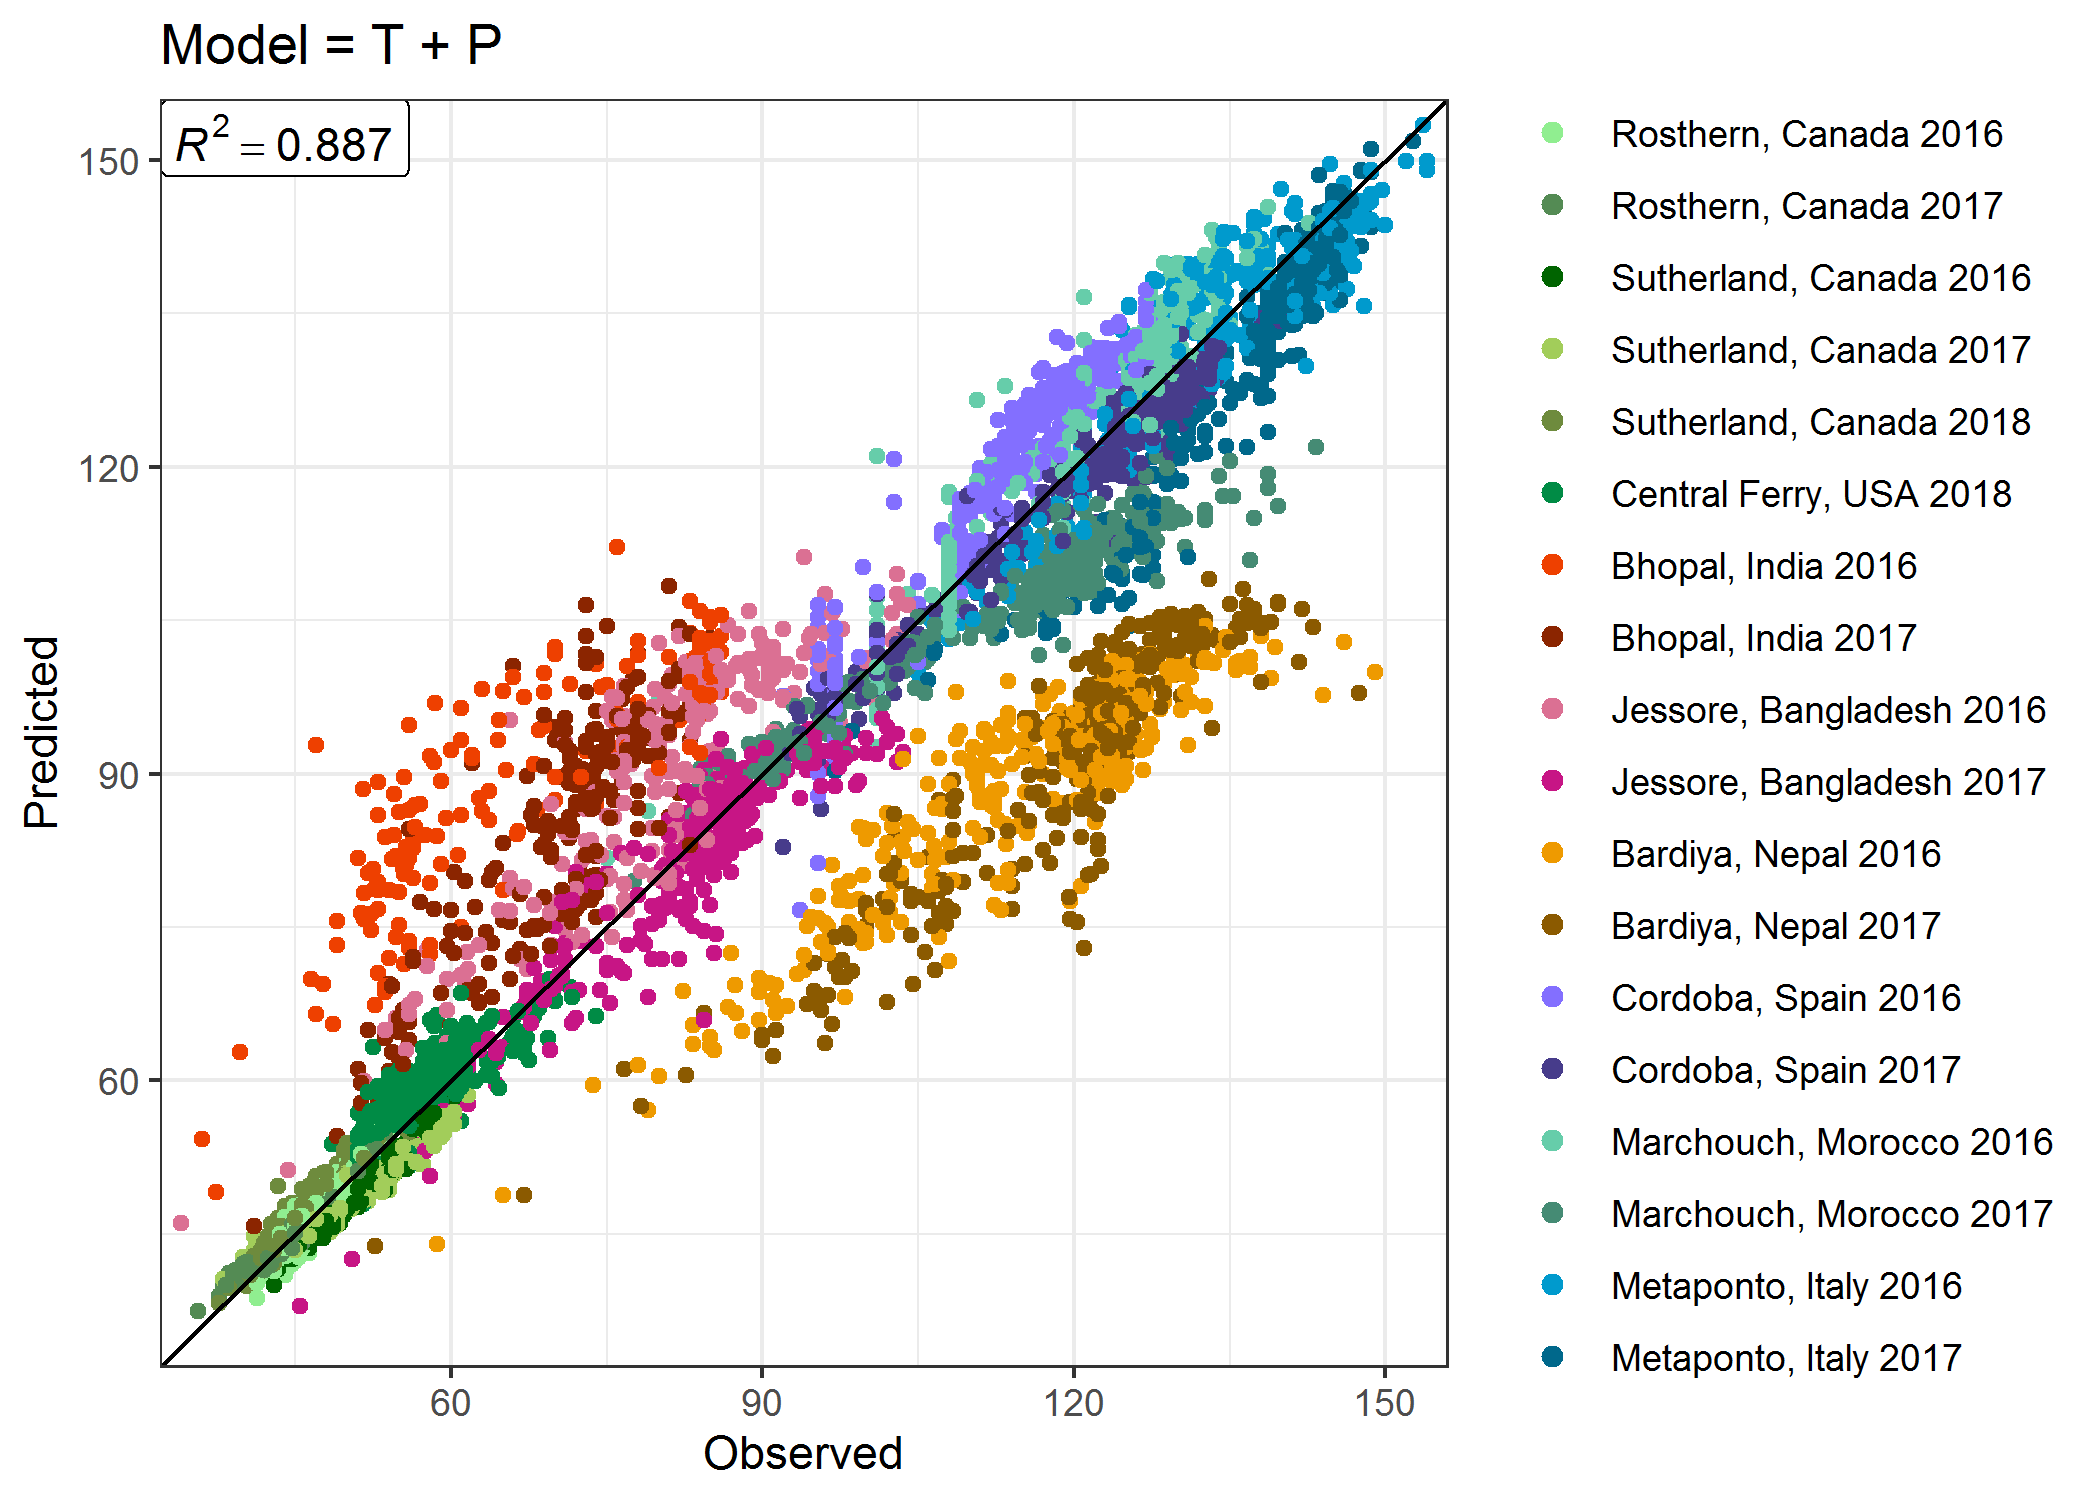
\includegraphics{Additional/Model/Model_1_1.png}

\begin{Shaded}
\begin{Highlighting}[]
\CommentTok{# Plot Observed vs Predicted}
\NormalTok{mp <-}\StringTok{ }\KeywordTok{gg_model_2}\NormalTok{(xx, }\DataTypeTok{title =} \StringTok{"Model = T + P"}\NormalTok{)}
\KeywordTok{ggsave}\NormalTok{(}\StringTok{"Additional/Model/Model_2_1.png"}\NormalTok{, mp, }\DataTypeTok{width =} \DecValTok{8}\NormalTok{, }\DataTypeTok{height =} \FloatTok{5.5}\NormalTok{, }\DataTypeTok{dpi =} \DecValTok{600}\NormalTok{)}
\end{Highlighting}
\end{Shaded}

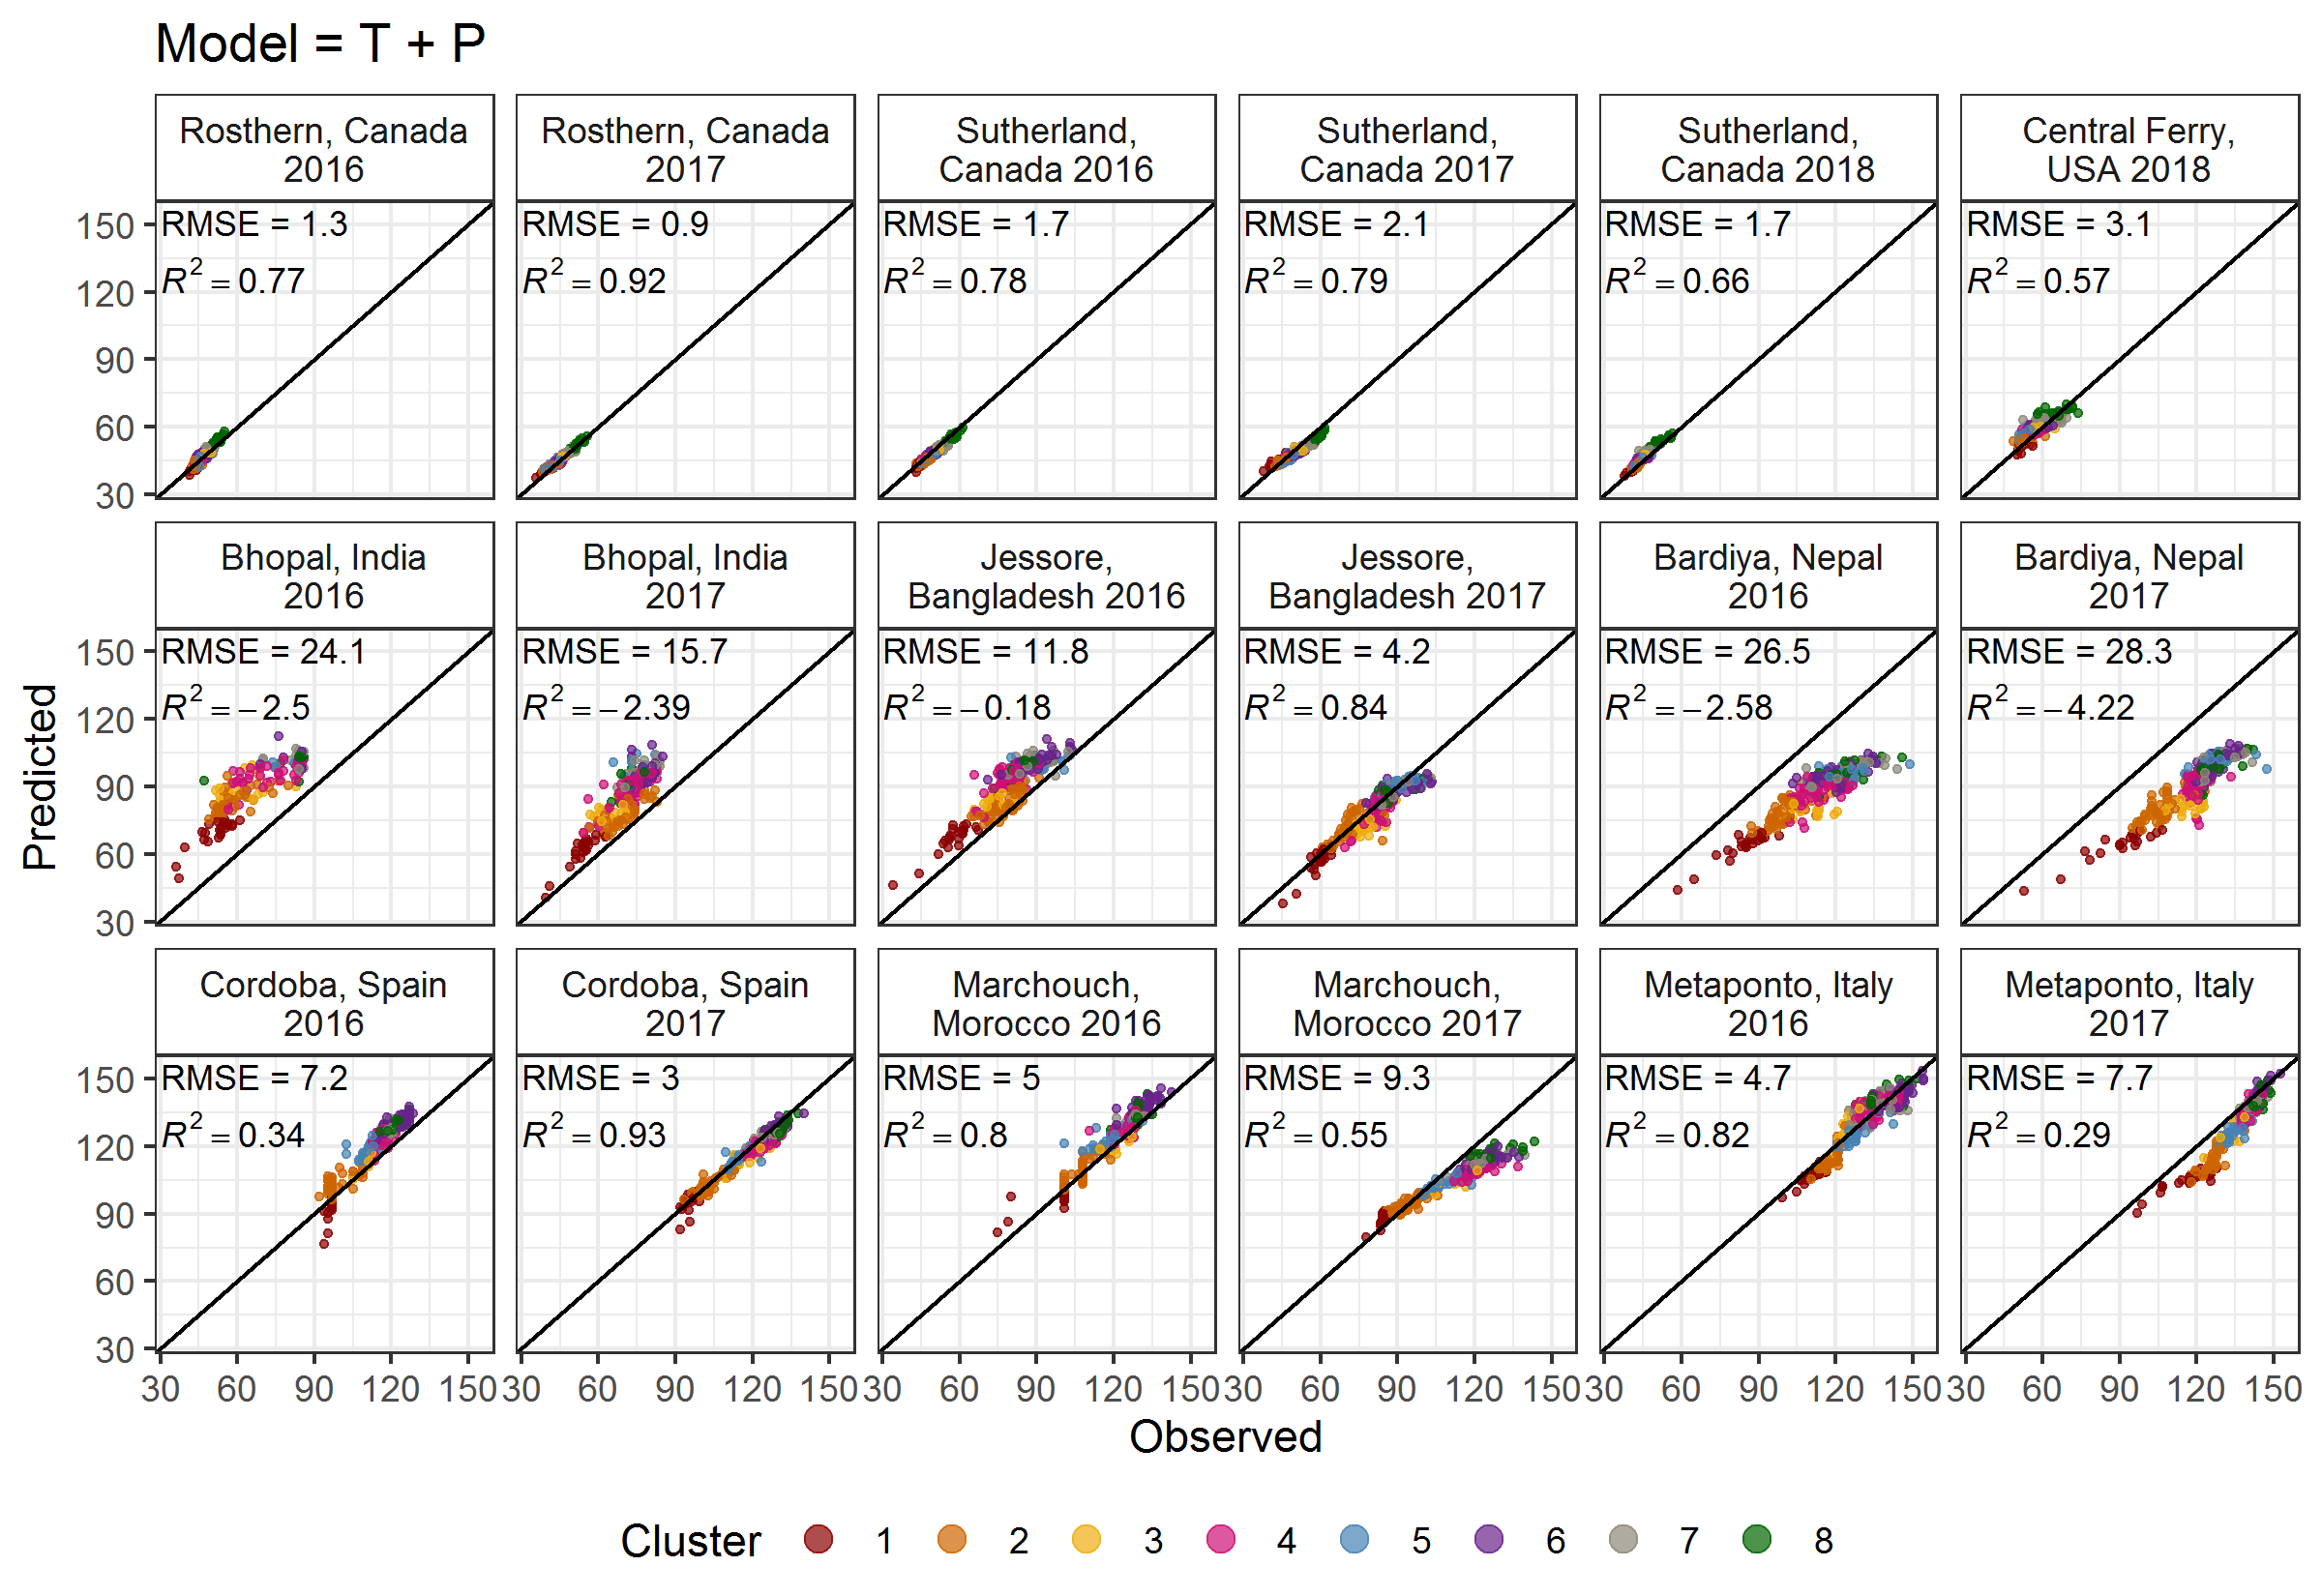
\includegraphics{Additional/Model/Model_2_1.png}

\begin{Shaded}
\begin{Highlighting}[]
\CommentTok{# Plot Observed vs Predicted for Temperate Locations}
\NormalTok{myexpts <-}\StringTok{ }\KeywordTok{c}\NormalTok{(}\StringTok{"Ro16"}\NormalTok{,}\StringTok{"Ro17"}\NormalTok{,}\StringTok{"Su16"}\NormalTok{,}\StringTok{"Su17"}\NormalTok{,}\StringTok{"Su18"}\NormalTok{,}\StringTok{"Us18"}\NormalTok{)}
\NormalTok{mp <-}\StringTok{ }\KeywordTok{gg_model_2}\NormalTok{(xx }\OperatorTok\StringTok{ }\KeywordTok{filter}\NormalTok{(ExptShort }\OperatorTok\StringTok{ }\NormalTok{myexpts))}
\KeywordTok{ggsave}\NormalTok{(}\StringTok{"Additional/Model/Model_3_1.png"}\NormalTok{, mp ,}\DataTypeTok{width =} \DecValTok{8}\NormalTok{, }\DataTypeTok{height =} \DecValTok{3}\NormalTok{, }\DataTypeTok{dpi =} \DecValTok{600}\NormalTok{)}
\end{Highlighting}
\end{Shaded}

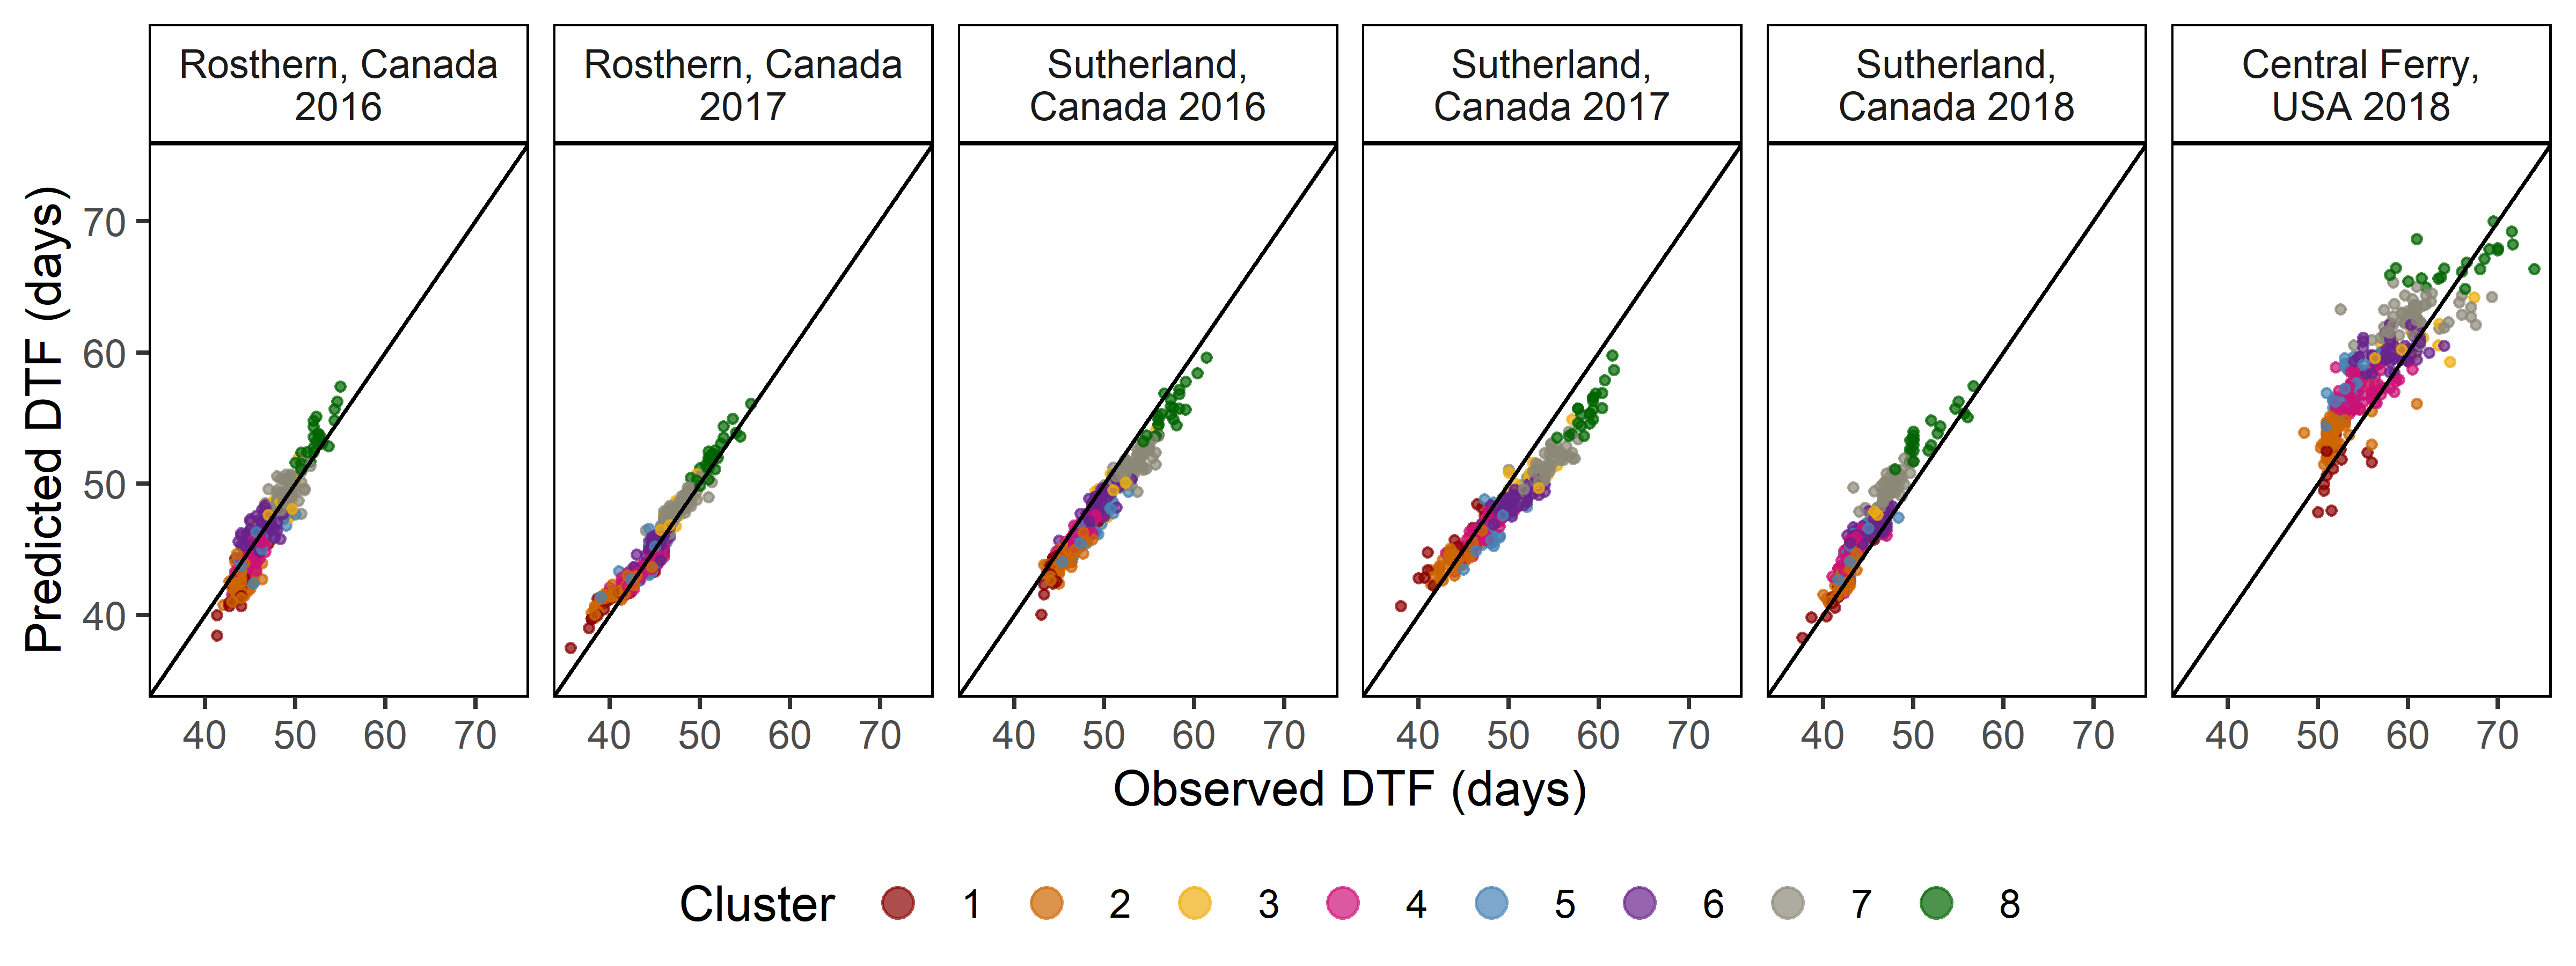
\includegraphics{Additional/Model/Model_3_1.png}

\hypertarget{modeling-dtf-t-x-p---all-site-years}{%
\subsection{Modeling DTF (T x P) - All
Site-years}\label{modeling-dtf-t-x-p---all-site-years}}

\begin{Shaded}
\begin{Highlighting}[]
\CommentTok{###########################}
\CommentTok{# 1/f = a + bT + cP (All) #}
\CommentTok{###########################}
\CommentTok{# Prep data}
\NormalTok{xx <-}\StringTok{ }\NormalTok{rr }\OperatorTok\StringTok{ }\KeywordTok{filter}\NormalTok{(}\OperatorTok{!}\KeywordTok{is.na}\NormalTok{(RDTF)) }\OperatorTok
\StringTok{  }\KeywordTok{left_join}\NormalTok{(}\KeywordTok{select}\NormalTok{(ff, Expt, T_mean, P_mean), }\DataTypeTok{by =} \StringTok{"Expt"}\NormalTok{) }\OperatorTok
\StringTok{  }\KeywordTok{select}\NormalTok{(Plot, Entry, Name, Rep, Expt, ExptShort, T_mean, P_mean, RDTF, DTF)}
\NormalTok{mr <-}\StringTok{ }\OtherTok{NULL}\NormalTok{; md <-}\StringTok{ }\OtherTok{NULL}
\NormalTok{mc <-}\StringTok{ }\KeywordTok{select}\NormalTok{(ldp, Entry, Name) }\OperatorTok
\StringTok{  }\KeywordTok{mutate}\NormalTok{(}\DataTypeTok{a =} \OtherTok{NA}\NormalTok{, }\DataTypeTok{b =} \OtherTok{NA}\NormalTok{, }\DataTypeTok{c =} \OtherTok{NA}\NormalTok{, }\DataTypeTok{d =} \OtherTok{NA}\NormalTok{, }\DataTypeTok{RR =} \OtherTok{NA}\NormalTok{, }\DataTypeTok{Environments =} \OtherTok{NA}\NormalTok{,}
         \DataTypeTok{aP =} \OtherTok{NA}\NormalTok{, }\DataTypeTok{bP =} \OtherTok{NA}\NormalTok{, }\DataTypeTok{cP=} \OtherTok{NA}\NormalTok{, }\DataTypeTok{dP =} \OtherTok{NA}\NormalTok{)}
\CommentTok{# Model}
\ControlFlowTok{for}\NormalTok{(i }\ControlFlowTok{in} \DecValTok{1}\OperatorTok{:}\DecValTok{324}\NormalTok{) \{}
  \CommentTok{# Prep data}
\NormalTok{  xri <-}\StringTok{ }\NormalTok{xx }\OperatorTok\StringTok{ }\KeywordTok{filter}\NormalTok{(Entry }\OperatorTok{==}\StringTok{ }\NormalTok{i)}
\NormalTok{  xdi <-}\StringTok{ }\NormalTok{xri }\OperatorTok\StringTok{ }\KeywordTok{group_by}\NormalTok{(Entry, Name, Expt, ExptShort) }\OperatorTok\StringTok{ }
\StringTok{    }\KeywordTok{summarise_at}\NormalTok{(}\KeywordTok{vars}\NormalTok{(DTF, RDTF, T_mean, P_mean), }\KeywordTok{funs}\NormalTok{(mean), }\DataTypeTok{na.rm =}\NormalTok{ T) }\OperatorTok
\StringTok{    }\KeywordTok{ungroup}\NormalTok{()}
  \CommentTok{# Train Model}
\NormalTok{  mi <-}\StringTok{ }\KeywordTok{lm}\NormalTok{(RDTF }\OperatorTok{~}\StringTok{ }\NormalTok{T_mean }\OperatorTok{*}\StringTok{ }\NormalTok{P_mean, }\DataTypeTok{data =}\NormalTok{ xri)}
  \CommentTok{# Predict DTF}
\NormalTok{  xri <-}\StringTok{ }\NormalTok{xri }\OperatorTok\StringTok{ }\KeywordTok{mutate}\NormalTok{(}\DataTypeTok{Predicted_RDTF =} \KeywordTok{predict}\NormalTok{(mi),}
                        \DataTypeTok{Predicted_DTF =} \DecValTok{1} \OperatorTok{/}\StringTok{ }\KeywordTok{predict}\NormalTok{(mi))}
\NormalTok{  xdi <-}\StringTok{ }\NormalTok{xdi }\OperatorTok\StringTok{ }\KeywordTok{mutate}\NormalTok{(}\DataTypeTok{Predicted_RDTF =} \KeywordTok{predict}\NormalTok{(mi, }\DataTypeTok{newdata =}\NormalTok{ xdi),}
                        \DataTypeTok{Predicted_DTF =} \DecValTok{1} \OperatorTok{/}\StringTok{ }\KeywordTok{predict}\NormalTok{(mi, }\DataTypeTok{newdata =}\NormalTok{ xdi))}
  \CommentTok{# Save to table}
\NormalTok{  mr <-}\StringTok{ }\KeywordTok{bind_rows}\NormalTok{(mr, xri) }
\NormalTok{  md <-}\StringTok{ }\KeywordTok{bind_rows}\NormalTok{(md, xdi)}
  \CommentTok{# Save coefficients}
\NormalTok{  mc[i,}\KeywordTok{c}\NormalTok{(}\StringTok{"a"}\NormalTok{,}\StringTok{"b"}\NormalTok{,}\StringTok{"c"}\NormalTok{,}\StringTok{"d"}\NormalTok{)] <-}\StringTok{ }\NormalTok{mi}\OperatorTok{$}\NormalTok{coefficients}
  \CommentTok{# Calculate rr and # of environments used}
\NormalTok{  mc[i,}\StringTok{"RR"}\NormalTok{] <-}\StringTok{ }\DecValTok{1} \OperatorTok{-}\StringTok{ }\KeywordTok{sum}\NormalTok{((xri}\OperatorTok{$}\NormalTok{DTF }\OperatorTok{-}\StringTok{ }\NormalTok{xri}\OperatorTok{$}\NormalTok{Predicted_DTF)}\OperatorTok{^}\DecValTok{2}\NormalTok{, }\DataTypeTok{na.rm =}\NormalTok{ T) }\OperatorTok{/}\StringTok{ }
\StringTok{    }\KeywordTok{sum}\NormalTok{((xri}\OperatorTok{$}\NormalTok{Predicted_DTF }\OperatorTok{-}\StringTok{ }\KeywordTok{mean}\NormalTok{(xri}\OperatorTok{$}\NormalTok{DTF, }\DataTypeTok{na.rm =}\NormalTok{ T))}\OperatorTok{^}\DecValTok{2}\NormalTok{, }\DataTypeTok{na.rm =}\NormalTok{ T)}
\NormalTok{  mc[i,}\StringTok{"Environments"}\NormalTok{] <-}\StringTok{ }\KeywordTok{length}\NormalTok{(}\KeywordTok{unique}\NormalTok{(xri}\OperatorTok{$}\NormalTok{Expt[}\OperatorTok{!}\KeywordTok{is.na}\NormalTok{(xri}\OperatorTok{$}\NormalTok{DTF)]))}
\NormalTok{  mc[i,}\StringTok{"aP"}\NormalTok{] <-}\StringTok{ }\KeywordTok{summary}\NormalTok{(mi)[[}\DecValTok{4}\NormalTok{]][}\DecValTok{1}\NormalTok{,}\DecValTok{4}\NormalTok{]}
\NormalTok{  mc[i,}\StringTok{"bP"}\NormalTok{] <-}\StringTok{ }\KeywordTok{summary}\NormalTok{(mi)[[}\DecValTok{4}\NormalTok{]][}\DecValTok{2}\NormalTok{,}\DecValTok{4}\NormalTok{]}
\NormalTok{  mc[i,}\StringTok{"cP"}\NormalTok{] <-}\StringTok{ }\KeywordTok{summary}\NormalTok{(mi)[[}\DecValTok{4}\NormalTok{]][}\DecValTok{3}\NormalTok{,}\DecValTok{4}\NormalTok{]}
\NormalTok{  mc[i,}\StringTok{"dP"}\NormalTok{] <-}\StringTok{ }\KeywordTok{summary}\NormalTok{(mi)[[}\DecValTok{4}\NormalTok{]][}\DecValTok{4}\NormalTok{,}\DecValTok{4}\NormalTok{]}
\NormalTok{\}}
\NormalTok{mr <-}\StringTok{ }\NormalTok{mr }\OperatorTok\StringTok{ }\KeywordTok{mutate}\NormalTok{(}\DataTypeTok{Expt =} \KeywordTok{factor}\NormalTok{(Expt, }\DataTypeTok{levels =}\NormalTok{ names_Expt))}
\NormalTok{md <-}\StringTok{ }\NormalTok{md }\OperatorTok\StringTok{ }\KeywordTok{mutate}\NormalTok{(}\DataTypeTok{Expt =} \KeywordTok{factor}\NormalTok{(Expt, }\DataTypeTok{levels =}\NormalTok{ names_Expt))}
\CommentTok{# Save Results}
\KeywordTok{write.csv}\NormalTok{(mr, }\StringTok{"data/model_txp.csv"}\NormalTok{,       }\DataTypeTok{row.names =}\NormalTok{ F)}
\KeywordTok{write.csv}\NormalTok{(md, }\StringTok{"data/model_txp_d.csv"}\NormalTok{,     }\DataTypeTok{row.names =}\NormalTok{ F)}
\KeywordTok{write.csv}\NormalTok{(mc, }\StringTok{"data/model_txp_coefs.csv"}\NormalTok{, }\DataTypeTok{row.names =}\NormalTok{ F)}
\end{Highlighting}
\end{Shaded}

\begin{Shaded}
\begin{Highlighting}[]
\CommentTok{# Prep data}
\NormalTok{xx <-}\StringTok{ }\KeywordTok{read.csv}\NormalTok{(}\StringTok{"data/model_txp_d.csv"}\NormalTok{) }\OperatorTok\StringTok{ }
\StringTok{  }\KeywordTok{mutate}\NormalTok{(}\DataTypeTok{Expt =} \KeywordTok{factor}\NormalTok{(Expt, }\DataTypeTok{levels =}\NormalTok{ names_Expt))}
\CommentTok{# Plot Observed vs Predicted}
\NormalTok{mp <-}\StringTok{ }\KeywordTok{gg_model_1}\NormalTok{(xx, }\DataTypeTok{title =} \StringTok{"Model = T x P"}\NormalTok{)}
\KeywordTok{ggsave}\NormalTok{(}\StringTok{"Additional/Model/Model_1_2.png"}\NormalTok{, mp, }\DataTypeTok{width =} \DecValTok{7}\NormalTok{, }\DataTypeTok{height =} \DecValTok{5}\NormalTok{, }\DataTypeTok{dpi =} \DecValTok{600}\NormalTok{)}
\end{Highlighting}
\end{Shaded}

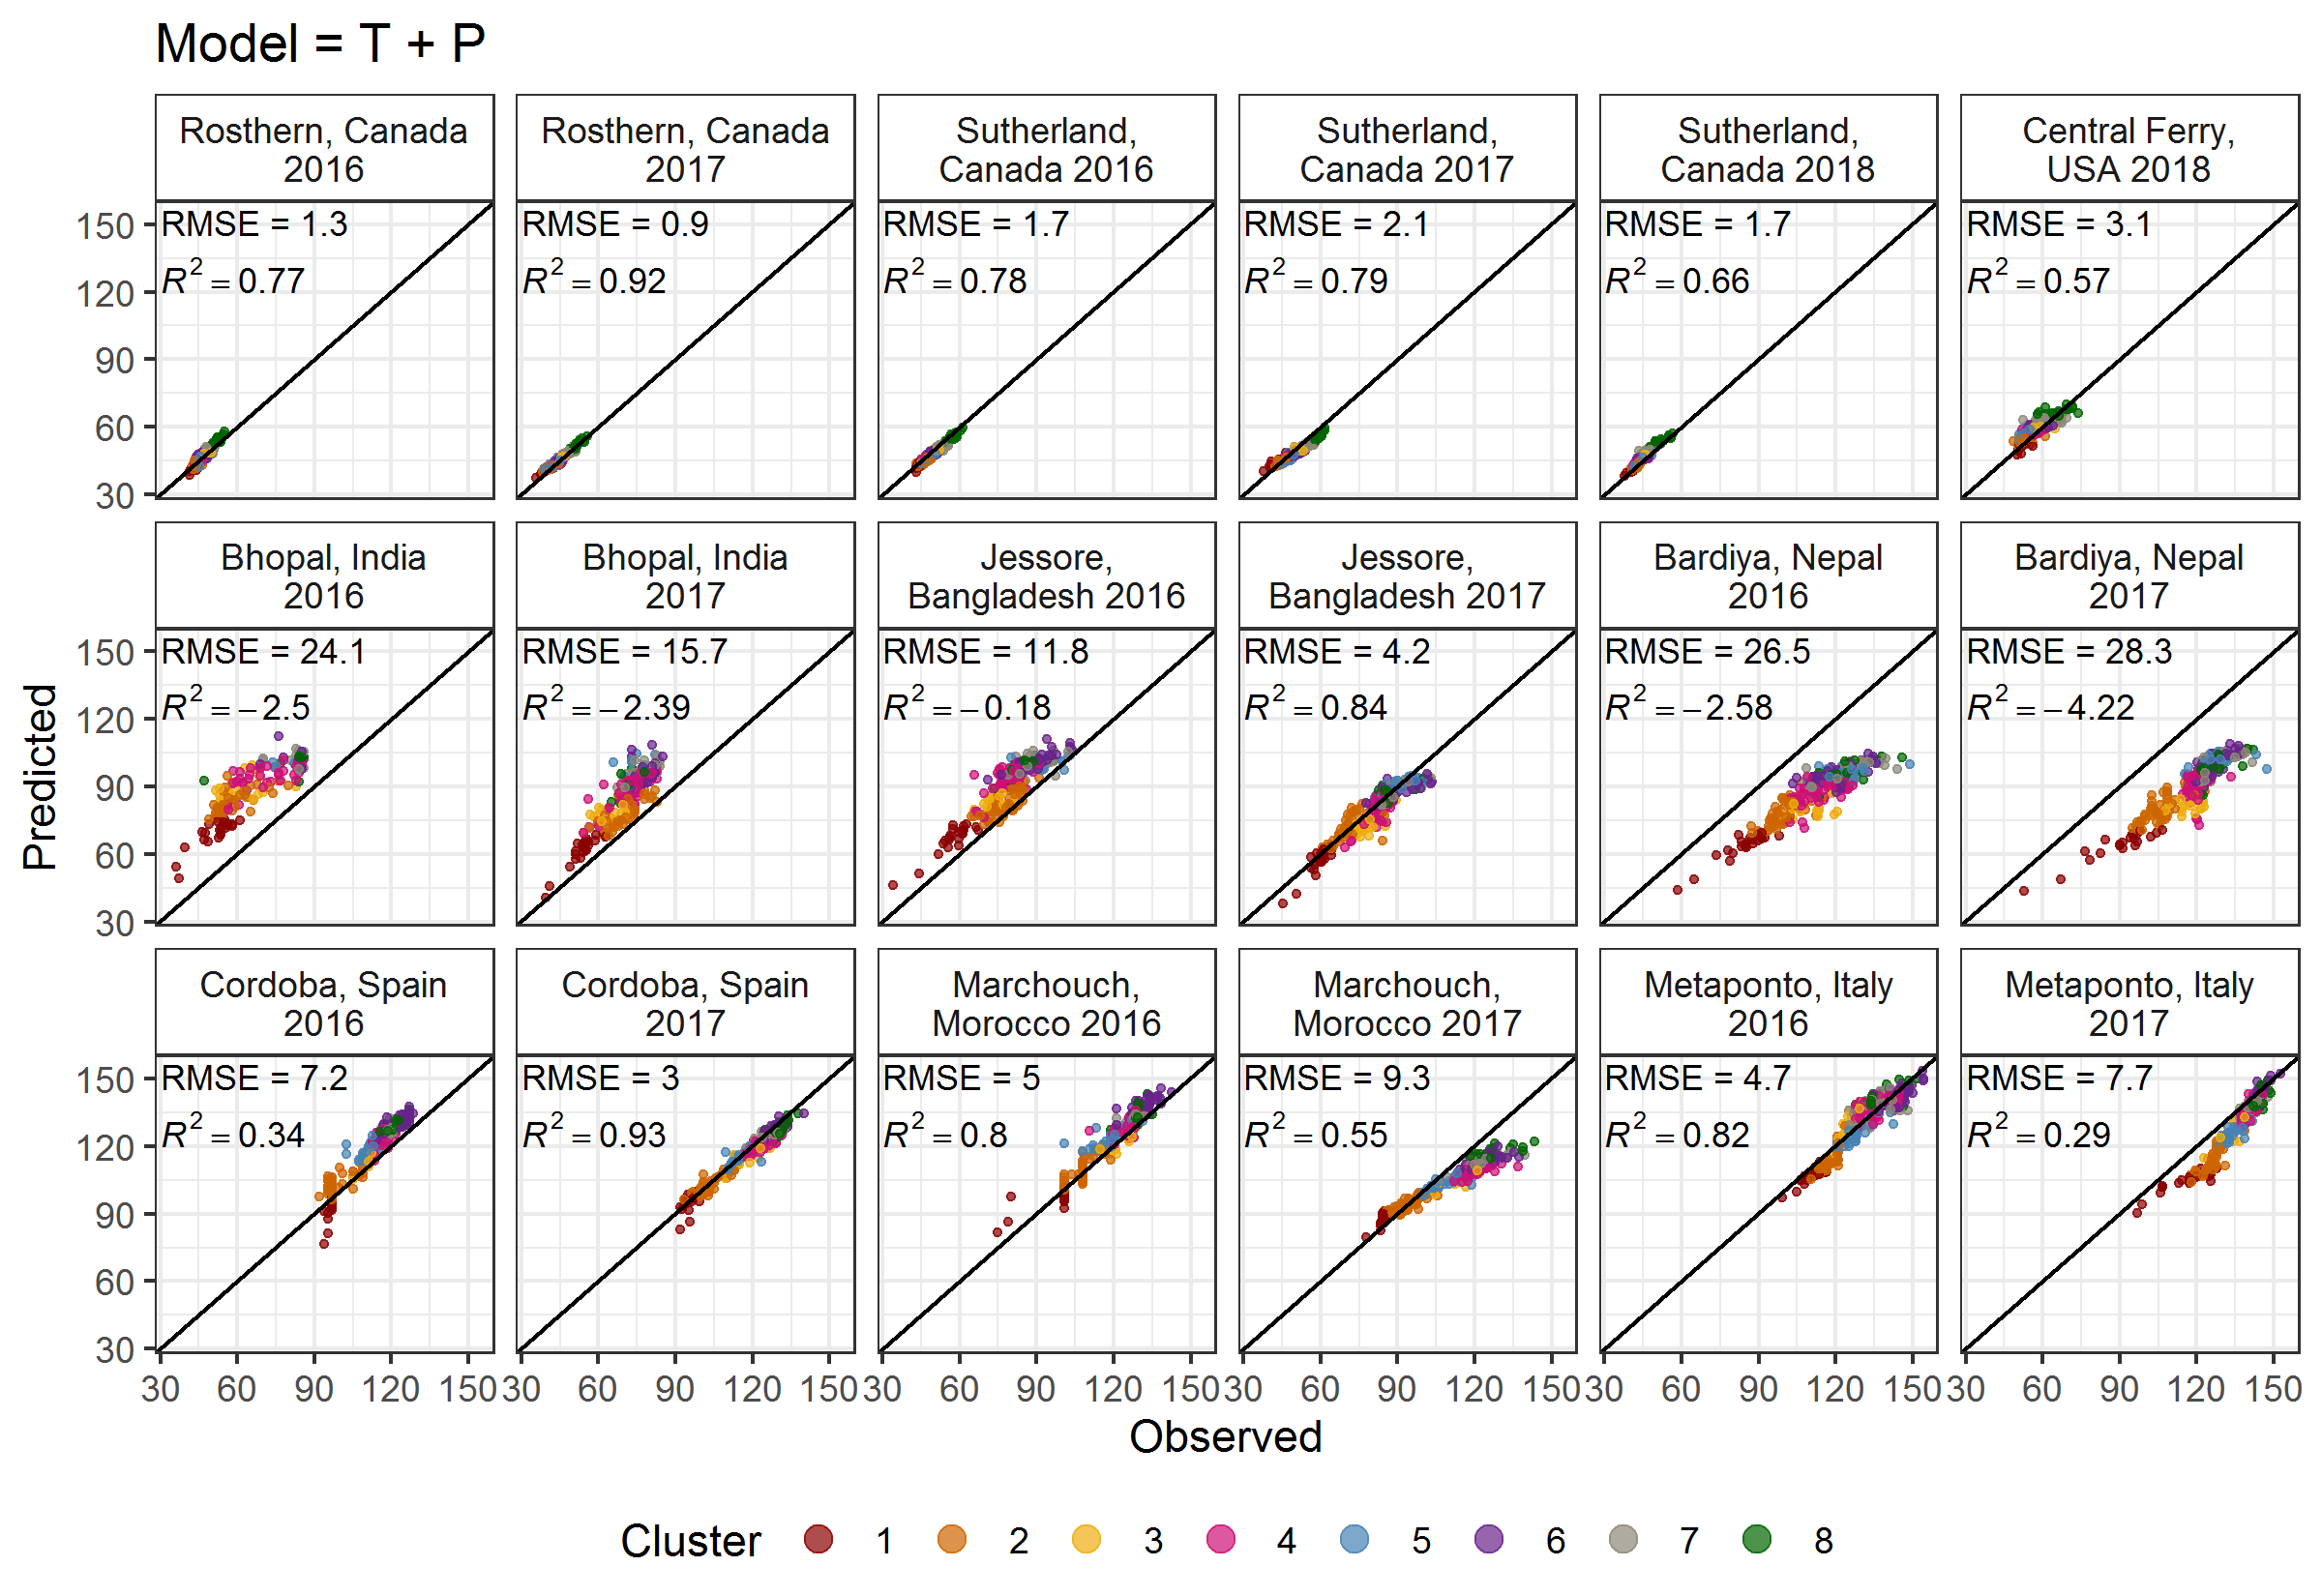
\includegraphics{Additional/Model/Model_2_1.png}

\begin{Shaded}
\begin{Highlighting}[]
\CommentTok{# Plot Observed vs Predicted}
\NormalTok{mp <-}\StringTok{ }\KeywordTok{gg_model_2}\NormalTok{(xx, }\DataTypeTok{title =} \StringTok{"Model = T x P"}\NormalTok{)}
\KeywordTok{ggsave}\NormalTok{(}\StringTok{"Additional/Model/Model_2_2.png"}\NormalTok{, mp, }\DataTypeTok{width =} \DecValTok{8}\NormalTok{, }\DataTypeTok{height =} \FloatTok{5.5}\NormalTok{, }\DataTypeTok{dpi =} \DecValTok{600}\NormalTok{)}
\end{Highlighting}
\end{Shaded}

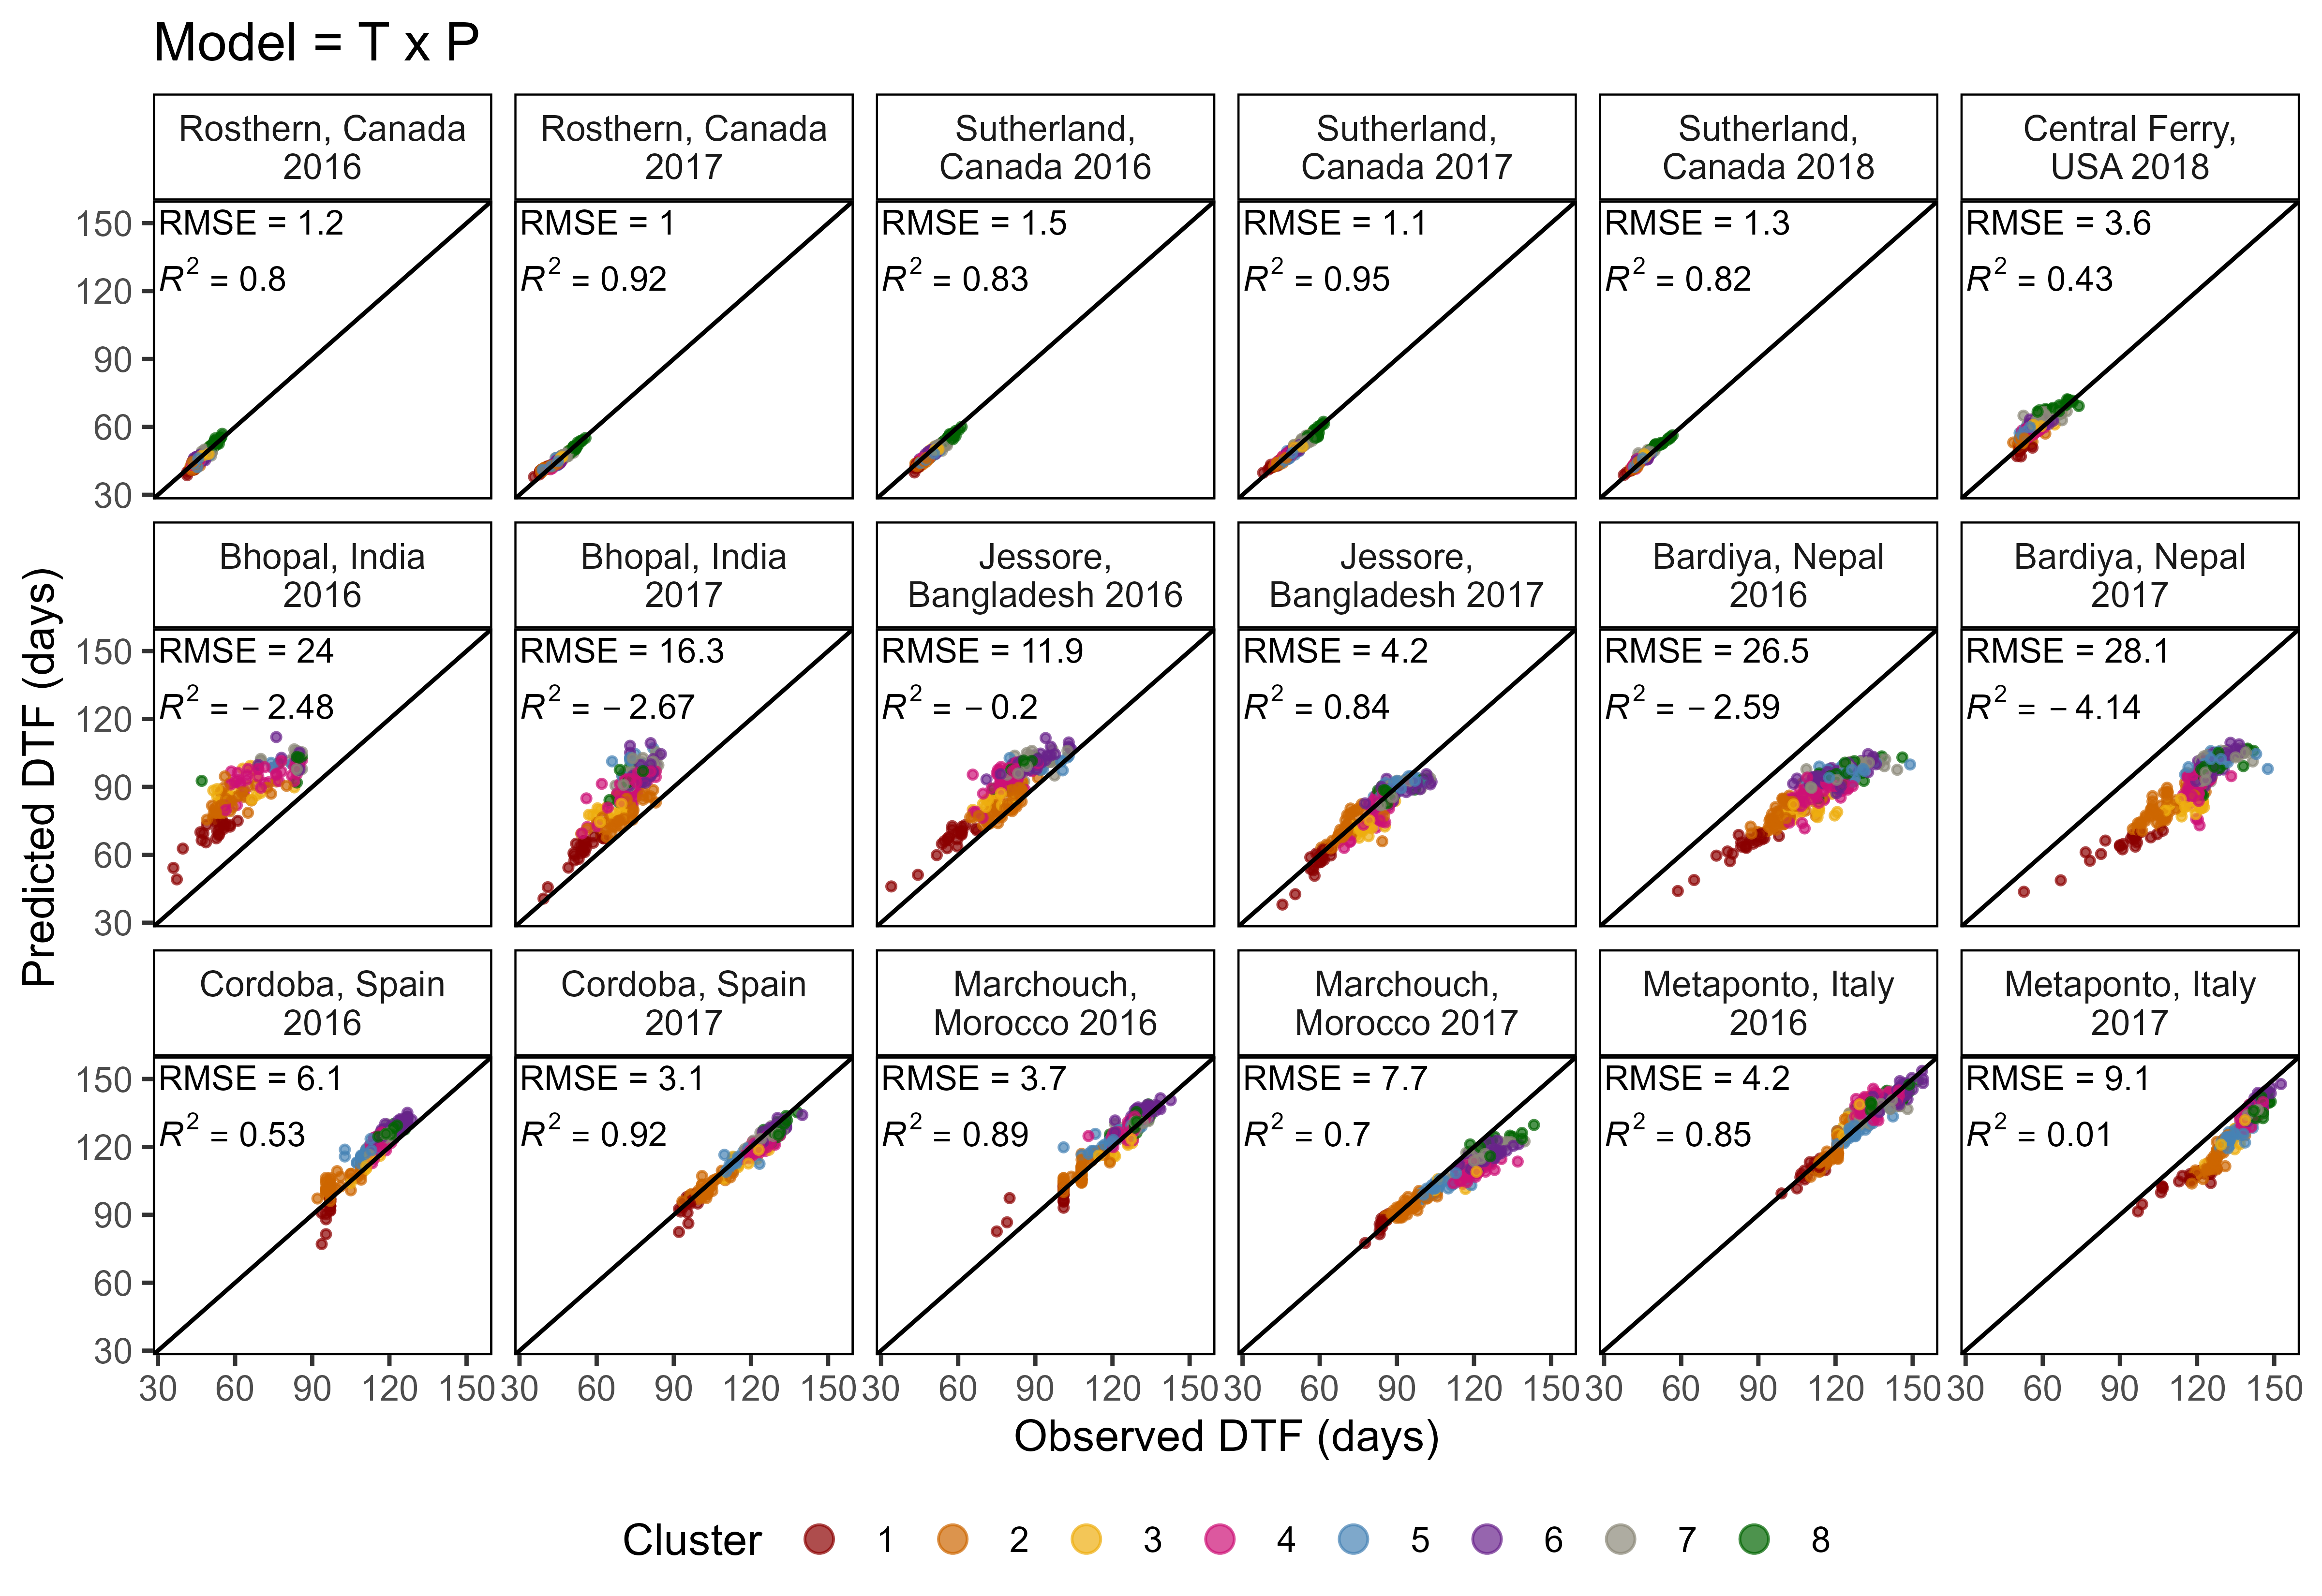
\includegraphics{Additional/Model/Model_2_2.png}

\hypertarget{supplemental-table-3-model-constants}{%
\subsection{Supplemental Table 3 Model
Constants}\label{supplemental-table-3-model-constants}}

\begin{Shaded}
\begin{Highlighting}[]
\CommentTok{# Prep data}
\NormalTok{x1 <-}\StringTok{ }\KeywordTok{read.csv}\NormalTok{(}\StringTok{"data/model_t+p_coefs.csv"}\NormalTok{)}
\NormalTok{x2 <-}\StringTok{ }\KeywordTok{read.csv}\NormalTok{(}\StringTok{"data/model_txp_coefs.csv"}\NormalTok{)}
\NormalTok{xx <-}\StringTok{ }\KeywordTok{bind_rows}\NormalTok{(x1, x2) }\OperatorTok\StringTok{ }\KeywordTok{arrange}\NormalTok{(Entry) }\OperatorTok\StringTok{ }
\StringTok{  }\KeywordTok{select}\NormalTok{(Entry, Name, a, b, c, d, RR, Environments, }
         \DataTypeTok{a_p.value=}\NormalTok{aP, }\DataTypeTok{b_p.value=}\NormalTok{bP, }\DataTypeTok{c_p.value=}\NormalTok{cP, }\DataTypeTok{d_p.value=}\NormalTok{dP)}
\CommentTok{# Save}
\KeywordTok{write.csv}\NormalTok{(xx, }\StringTok{"Supplemental_Table_03.csv"}\NormalTok{, }\DataTypeTok{na =} \StringTok{""}\NormalTok{, }\DataTypeTok{row.names =}\NormalTok{ F)}
\end{Highlighting}
\end{Shaded}

\begin{verbatim}
'data.frame':   648 obs. of  12 variables:
 $ Entry       : int  1 1 2 2 3 3 4 4 5 5 ...
 $ Name        : Factor w/ 324 levels "3156-11 AGL",..: 2 2 19 19 1 1 6 6 3 3 ...
 $ a           : num  -0.01877 0.00727 -0.01468 0.02093 -0.01388 ...
 $ b           : num  0.000337 -0.001202 0.000352 -0.001752 0.000356 ...
 $ c           : num  0.002046 -0.000317 0.001691 -0.001534 0.001587 ...
 $ d           : num  NA 0.00014 NA 0.000191 NA ...
 $ RR          : num  0.898 0.899 0.846 0.843 0.883 ...
 $ Environments: int  16 16 18 18 16 16 17 17 17 17 ...
 $ a_p.value   : num  2.41e-21 6.20e-01 1.99e-15 1.69e-01 3.05e-18 ...
 $ b_p.value   : num  5.43e-08 1.69e-01 2.76e-07 5.34e-02 3.33e-10 ...
 $ c_p.value   : num  3.68e-31 8.11e-01 1.07e-24 2.63e-01 4.76e-29 ...
 $ d_p.value   : num  NA 0.0794 NA 0.0213 NA ...
\end{verbatim}

\hypertarget{additional-figure-10-significant-t-x-p-interactions}{%
\subsection{Additional Figure 10 significant T x P
interactions}\label{additional-figure-10-significant-t-x-p-interactions}}

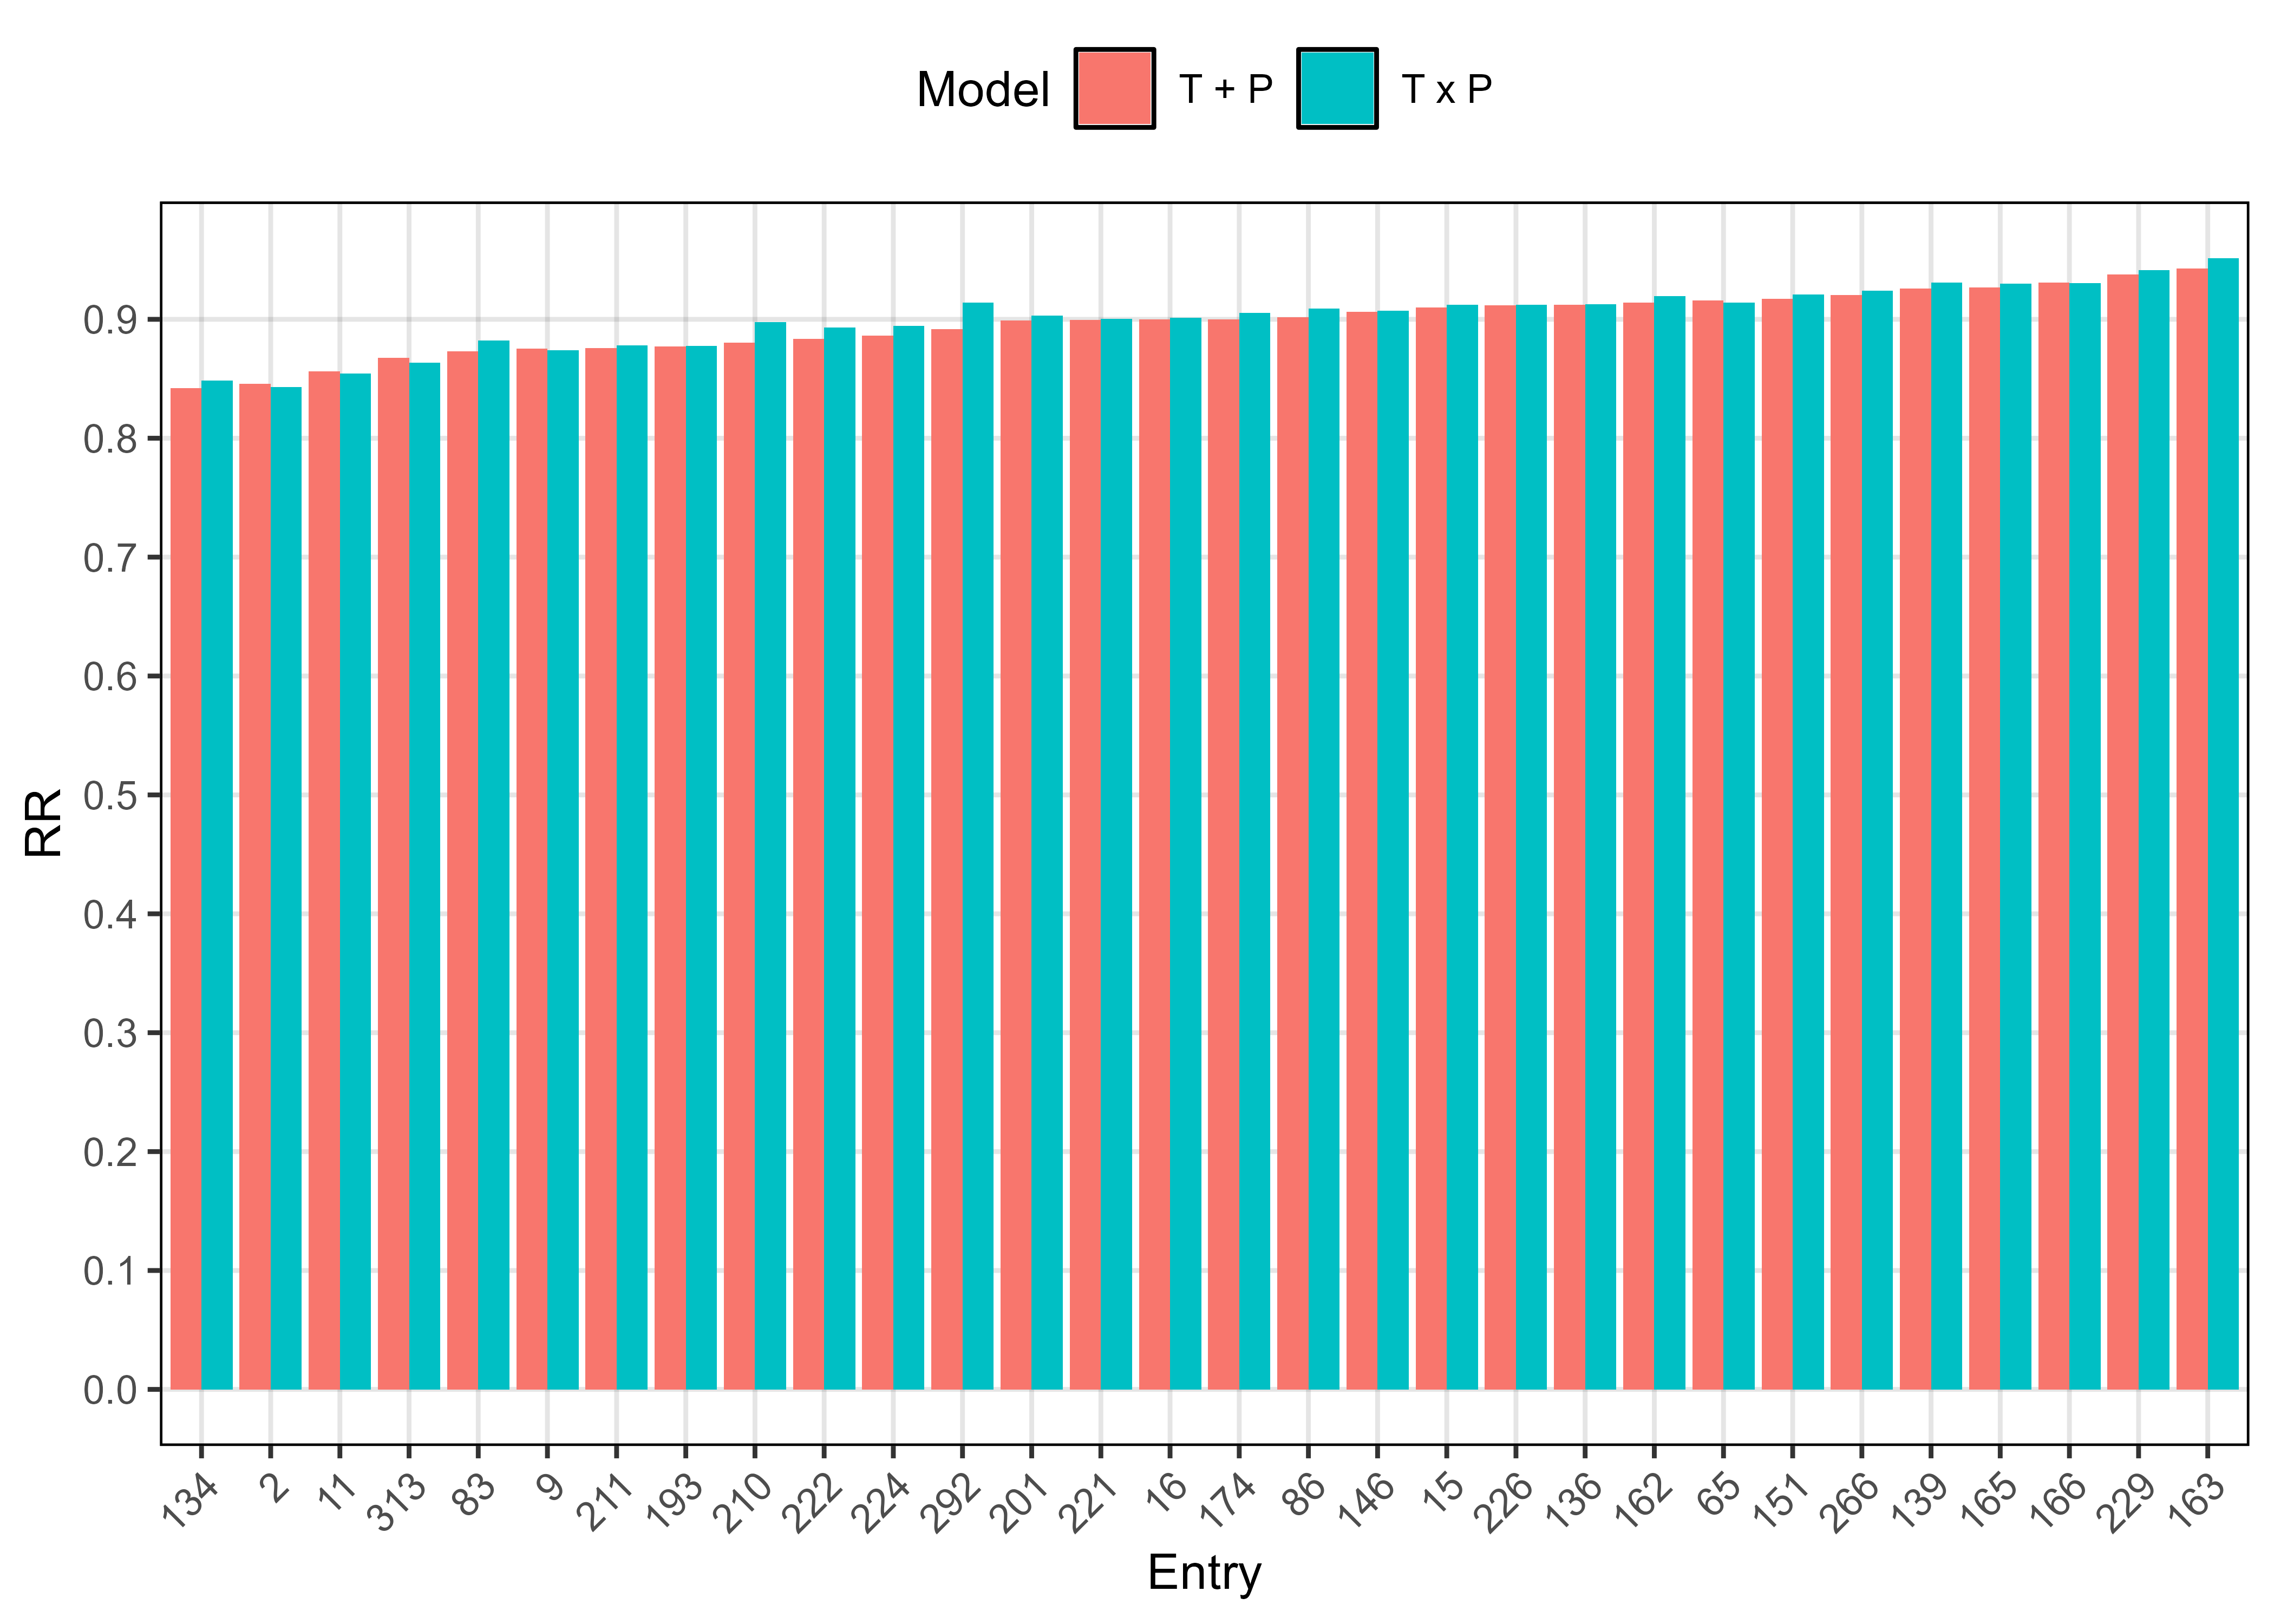
\includegraphics{Additional/Additional_Figure_10.png}

\begin{Shaded}
\begin{Highlighting}[]
\CommentTok{# Prep data}
\NormalTok{ents <-}\StringTok{ }\NormalTok{x2 }\OperatorTok\StringTok{ }\KeywordTok{filter}\NormalTok{(dP }\OperatorTok{<}\StringTok{ }\FloatTok{0.05}\NormalTok{) }\OperatorTok\StringTok{ }\KeywordTok{pull}\NormalTok{(Entry)}
\NormalTok{xx <-}\StringTok{ }\NormalTok{xx }\OperatorTok\StringTok{ }\KeywordTok{filter}\NormalTok{(Entry }\OperatorTok\StringTok{ }\NormalTok{ents)}
\NormalTok{xx <-}\StringTok{ }\NormalTok{xx }\OperatorTok\StringTok{ }\KeywordTok{arrange}\NormalTok{(RR) }\OperatorTok\StringTok{ }
\StringTok{  }\KeywordTok{mutate}\NormalTok{(}\DataTypeTok{Entry =} \KeywordTok{factor}\NormalTok{(Entry, }\DataTypeTok{levels =} \KeywordTok{unique}\NormalTok{(Entry)),}
         \DataTypeTok{Model =} \KeywordTok{ifelse}\NormalTok{(}\KeywordTok{is.na}\NormalTok{(d), }\StringTok{"T + P"}\NormalTok{, }\StringTok{"T x P"}\NormalTok{))}
\KeywordTok{length}\NormalTok{(ents)}
\end{Highlighting}
\end{Shaded}

\begin{verbatim}
[1] 30
\end{verbatim}

\begin{Shaded}
\begin{Highlighting}[]
\CommentTok{# Plot}
\NormalTok{mp <-}\StringTok{ }\KeywordTok{ggplot}\NormalTok{(xx, }\KeywordTok{aes}\NormalTok{(}\DataTypeTok{x =}\NormalTok{ Entry, }\DataTypeTok{y =}\NormalTok{ RR, }\DataTypeTok{fill =}\NormalTok{ Model)) }\OperatorTok{+}\StringTok{ }
\StringTok{  }\KeywordTok{geom_bar}\NormalTok{(}\DataTypeTok{stat =} \StringTok{"identity"}\NormalTok{, }\DataTypeTok{position =} \StringTok{"dodge"}\NormalTok{) }\OperatorTok{+}
\StringTok{  }\KeywordTok{scale_y_continuous}\NormalTok{(}\DataTypeTok{breaks =} \KeywordTok{seq}\NormalTok{(}\DecValTok{0}\NormalTok{,}\DecValTok{1}\NormalTok{,}\FloatTok{0.1}\NormalTok{), }\DataTypeTok{minor_breaks =} \KeywordTok{seq}\NormalTok{(}\DecValTok{0}\NormalTok{,}\DecValTok{1}\NormalTok{,}\FloatTok{0.01}\NormalTok{)) }\OperatorTok{+}
\StringTok{  }\NormalTok{theme_AGL }\OperatorTok{+}\StringTok{ }
\StringTok{  }\KeywordTok{theme}\NormalTok{(}\DataTypeTok{legend.position =} \StringTok{"top"}\NormalTok{) }
\KeywordTok{ggsave}\NormalTok{(}\StringTok{"Additional/Additional_Figure_10.png"}\NormalTok{, mp, }\DataTypeTok{width =} \DecValTok{7}\NormalTok{, }\DataTypeTok{height =} \DecValTok{5}\NormalTok{, }\DataTypeTok{dpi =} \DecValTok{600}\NormalTok{)}
\end{Highlighting}
\end{Shaded}

\hypertarget{supplemental-figure-5-model-t-p-vs-t-x-p}{%
\subsection{Supplemental Figure 5 Model T + P vs T x
P}\label{supplemental-figure-5-model-t-p-vs-t-x-p}}

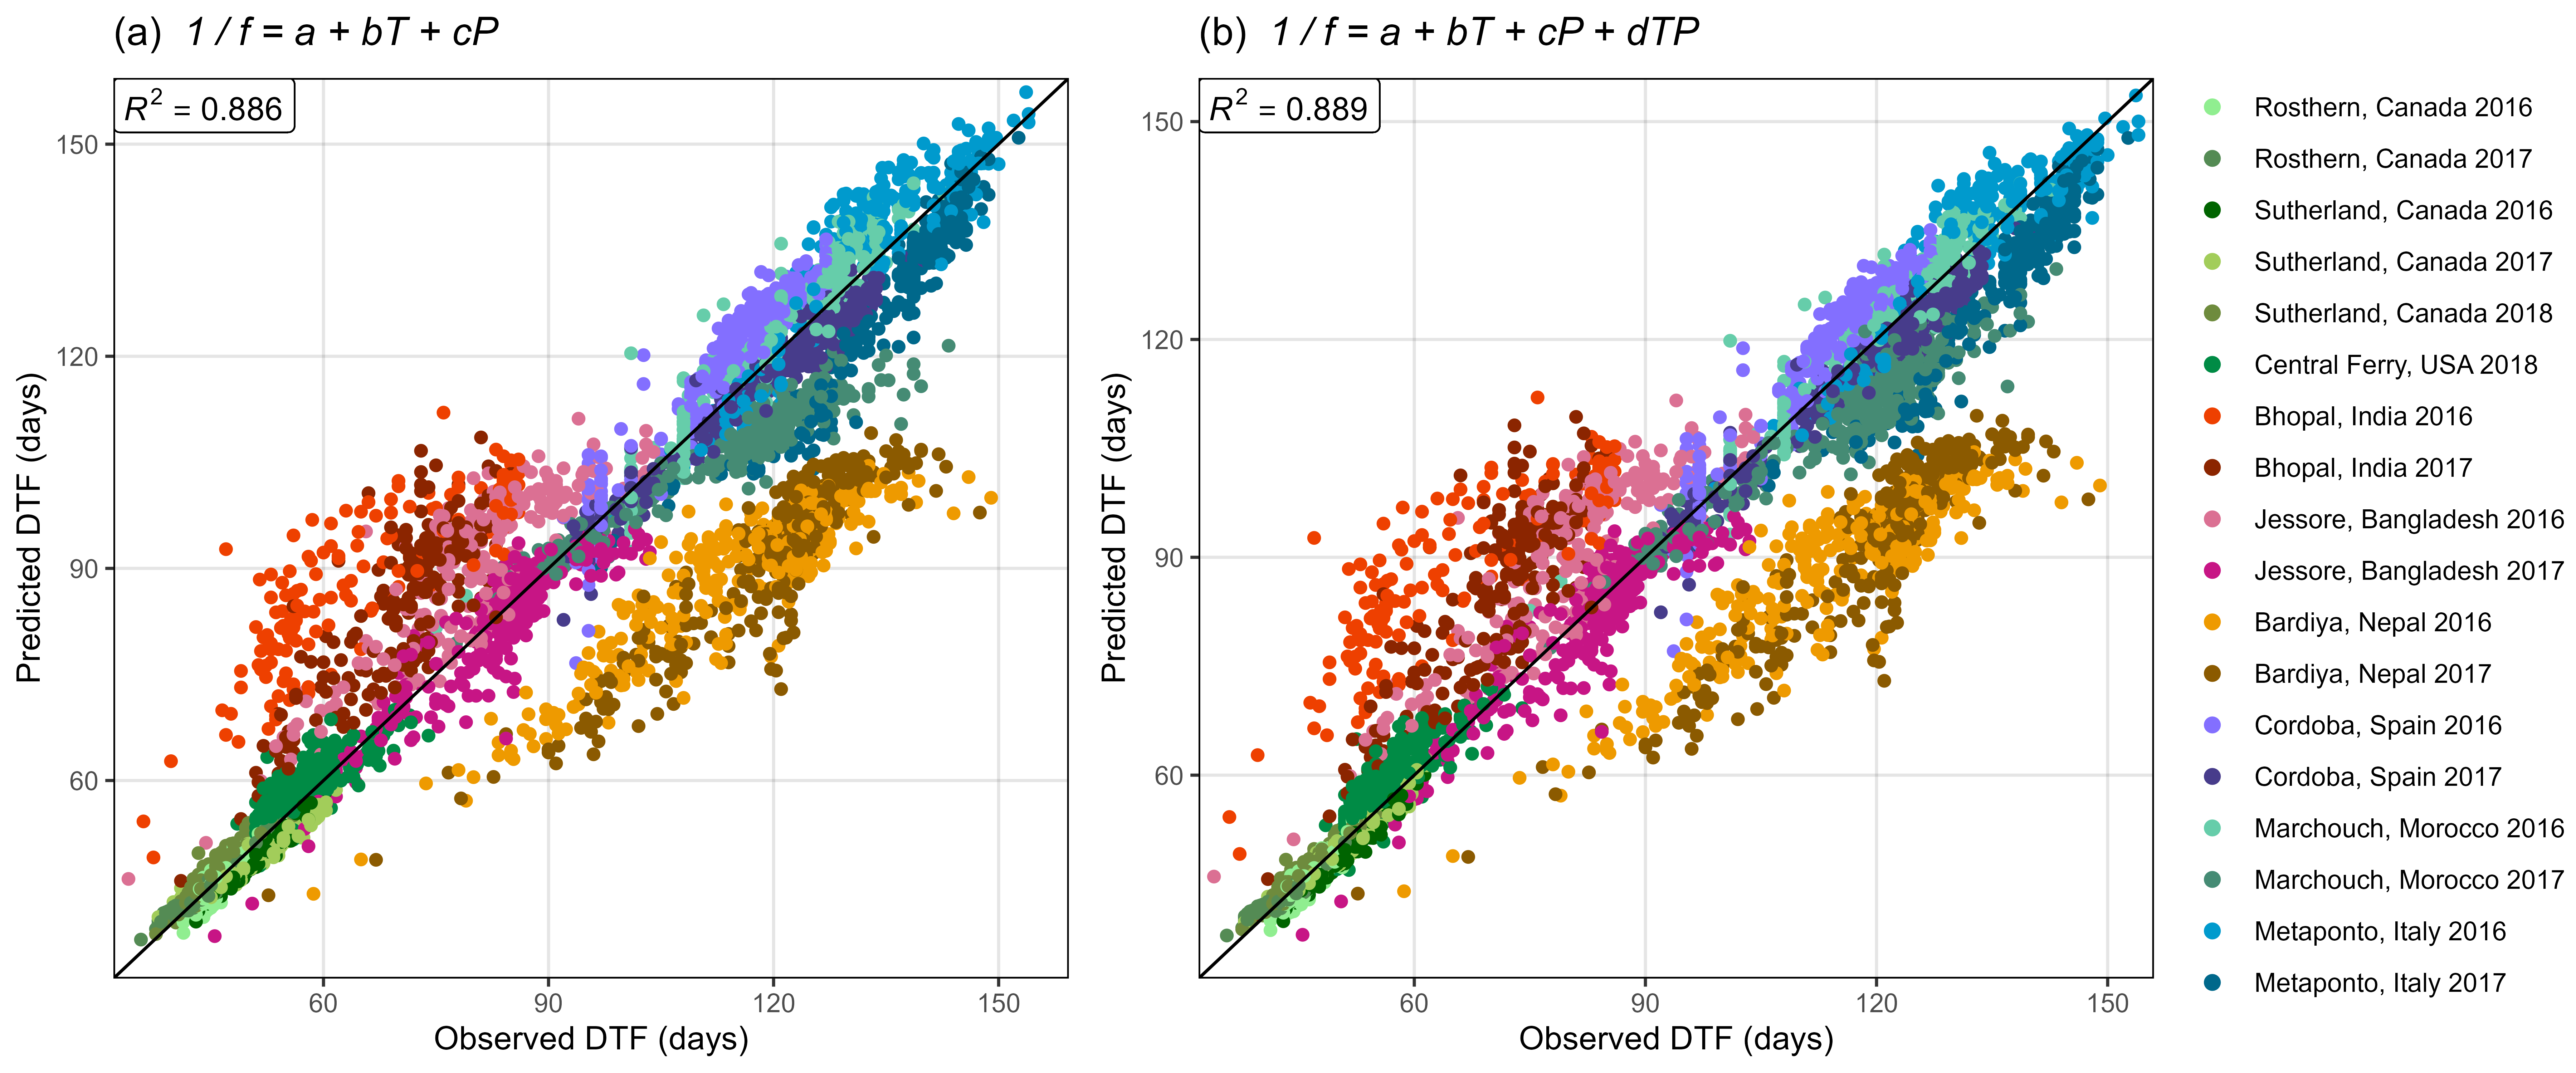
\includegraphics{Supplemental_Figure_05.png}

\begin{Shaded}
\begin{Highlighting}[]
\CommentTok{# Prep data}
\NormalTok{xx <-}\StringTok{ }\KeywordTok{read.csv}\NormalTok{(}\StringTok{"data/model_t+p_d.csv"}\NormalTok{) }\OperatorTok\StringTok{ }
\StringTok{  }\KeywordTok{mutate}\NormalTok{(}\DataTypeTok{Expt =} \KeywordTok{factor}\NormalTok{(Expt, }\DataTypeTok{levels =}\NormalTok{ names_Expt))}
\CommentTok{# Plot Observed vs Predicted}
\NormalTok{mp1 <-}\StringTok{ }\KeywordTok{gg_model_1}\NormalTok{(xx, }
  \DataTypeTok{title =} \KeywordTok{expression}\NormalTok{(}\KeywordTok{paste}\NormalTok{(}\StringTok{"(a) "}\NormalTok{, }\KeywordTok{italic}\NormalTok{(}\StringTok{" 1 / f = a + bT + cP"}\NormalTok{))))}
\CommentTok{# Prep data}
\NormalTok{xx <-}\StringTok{ }\KeywordTok{read.csv}\NormalTok{(}\StringTok{"data/model_txp_d.csv"}\NormalTok{) }\OperatorTok\StringTok{ }
\StringTok{  }\KeywordTok{mutate}\NormalTok{(}\DataTypeTok{Expt =} \KeywordTok{factor}\NormalTok{(Expt, }\DataTypeTok{levels =}\NormalTok{ names_Expt))}
\CommentTok{# Plot Observed vs Predicted}
\NormalTok{mp2 <-}\StringTok{ }\KeywordTok{gg_model_1}\NormalTok{(xx, }
  \DataTypeTok{title =} \KeywordTok{expression}\NormalTok{(}\KeywordTok{paste}\NormalTok{(}\StringTok{"(b) "}\NormalTok{, }\KeywordTok{italic}\NormalTok{(}\StringTok{" 1 / f = a + bT + cP + dTP"}\NormalTok{))))}
\CommentTok{# Append}
\NormalTok{mp <-}\StringTok{ }\KeywordTok{ggarrange}\NormalTok{(mp1, mp2, }\DataTypeTok{ncol =} \DecValTok{2}\NormalTok{, }\DataTypeTok{common.legend =}\NormalTok{ T, }\DataTypeTok{legend =} \StringTok{"right"}\NormalTok{)}
\KeywordTok{ggsave}\NormalTok{(}\StringTok{"Supplemental_Figure_05.png"}\NormalTok{, mp, }\DataTypeTok{width =} \DecValTok{12}\NormalTok{, }\DataTypeTok{height =} \DecValTok{5}\NormalTok{, }\DataTypeTok{dpi =} \DecValTok{600}\NormalTok{)}
\end{Highlighting}
\end{Shaded}

\hypertarget{additional-figure-11-constants}{%
\subsection{Additional Figure 11
Constants}\label{additional-figure-11-constants}}

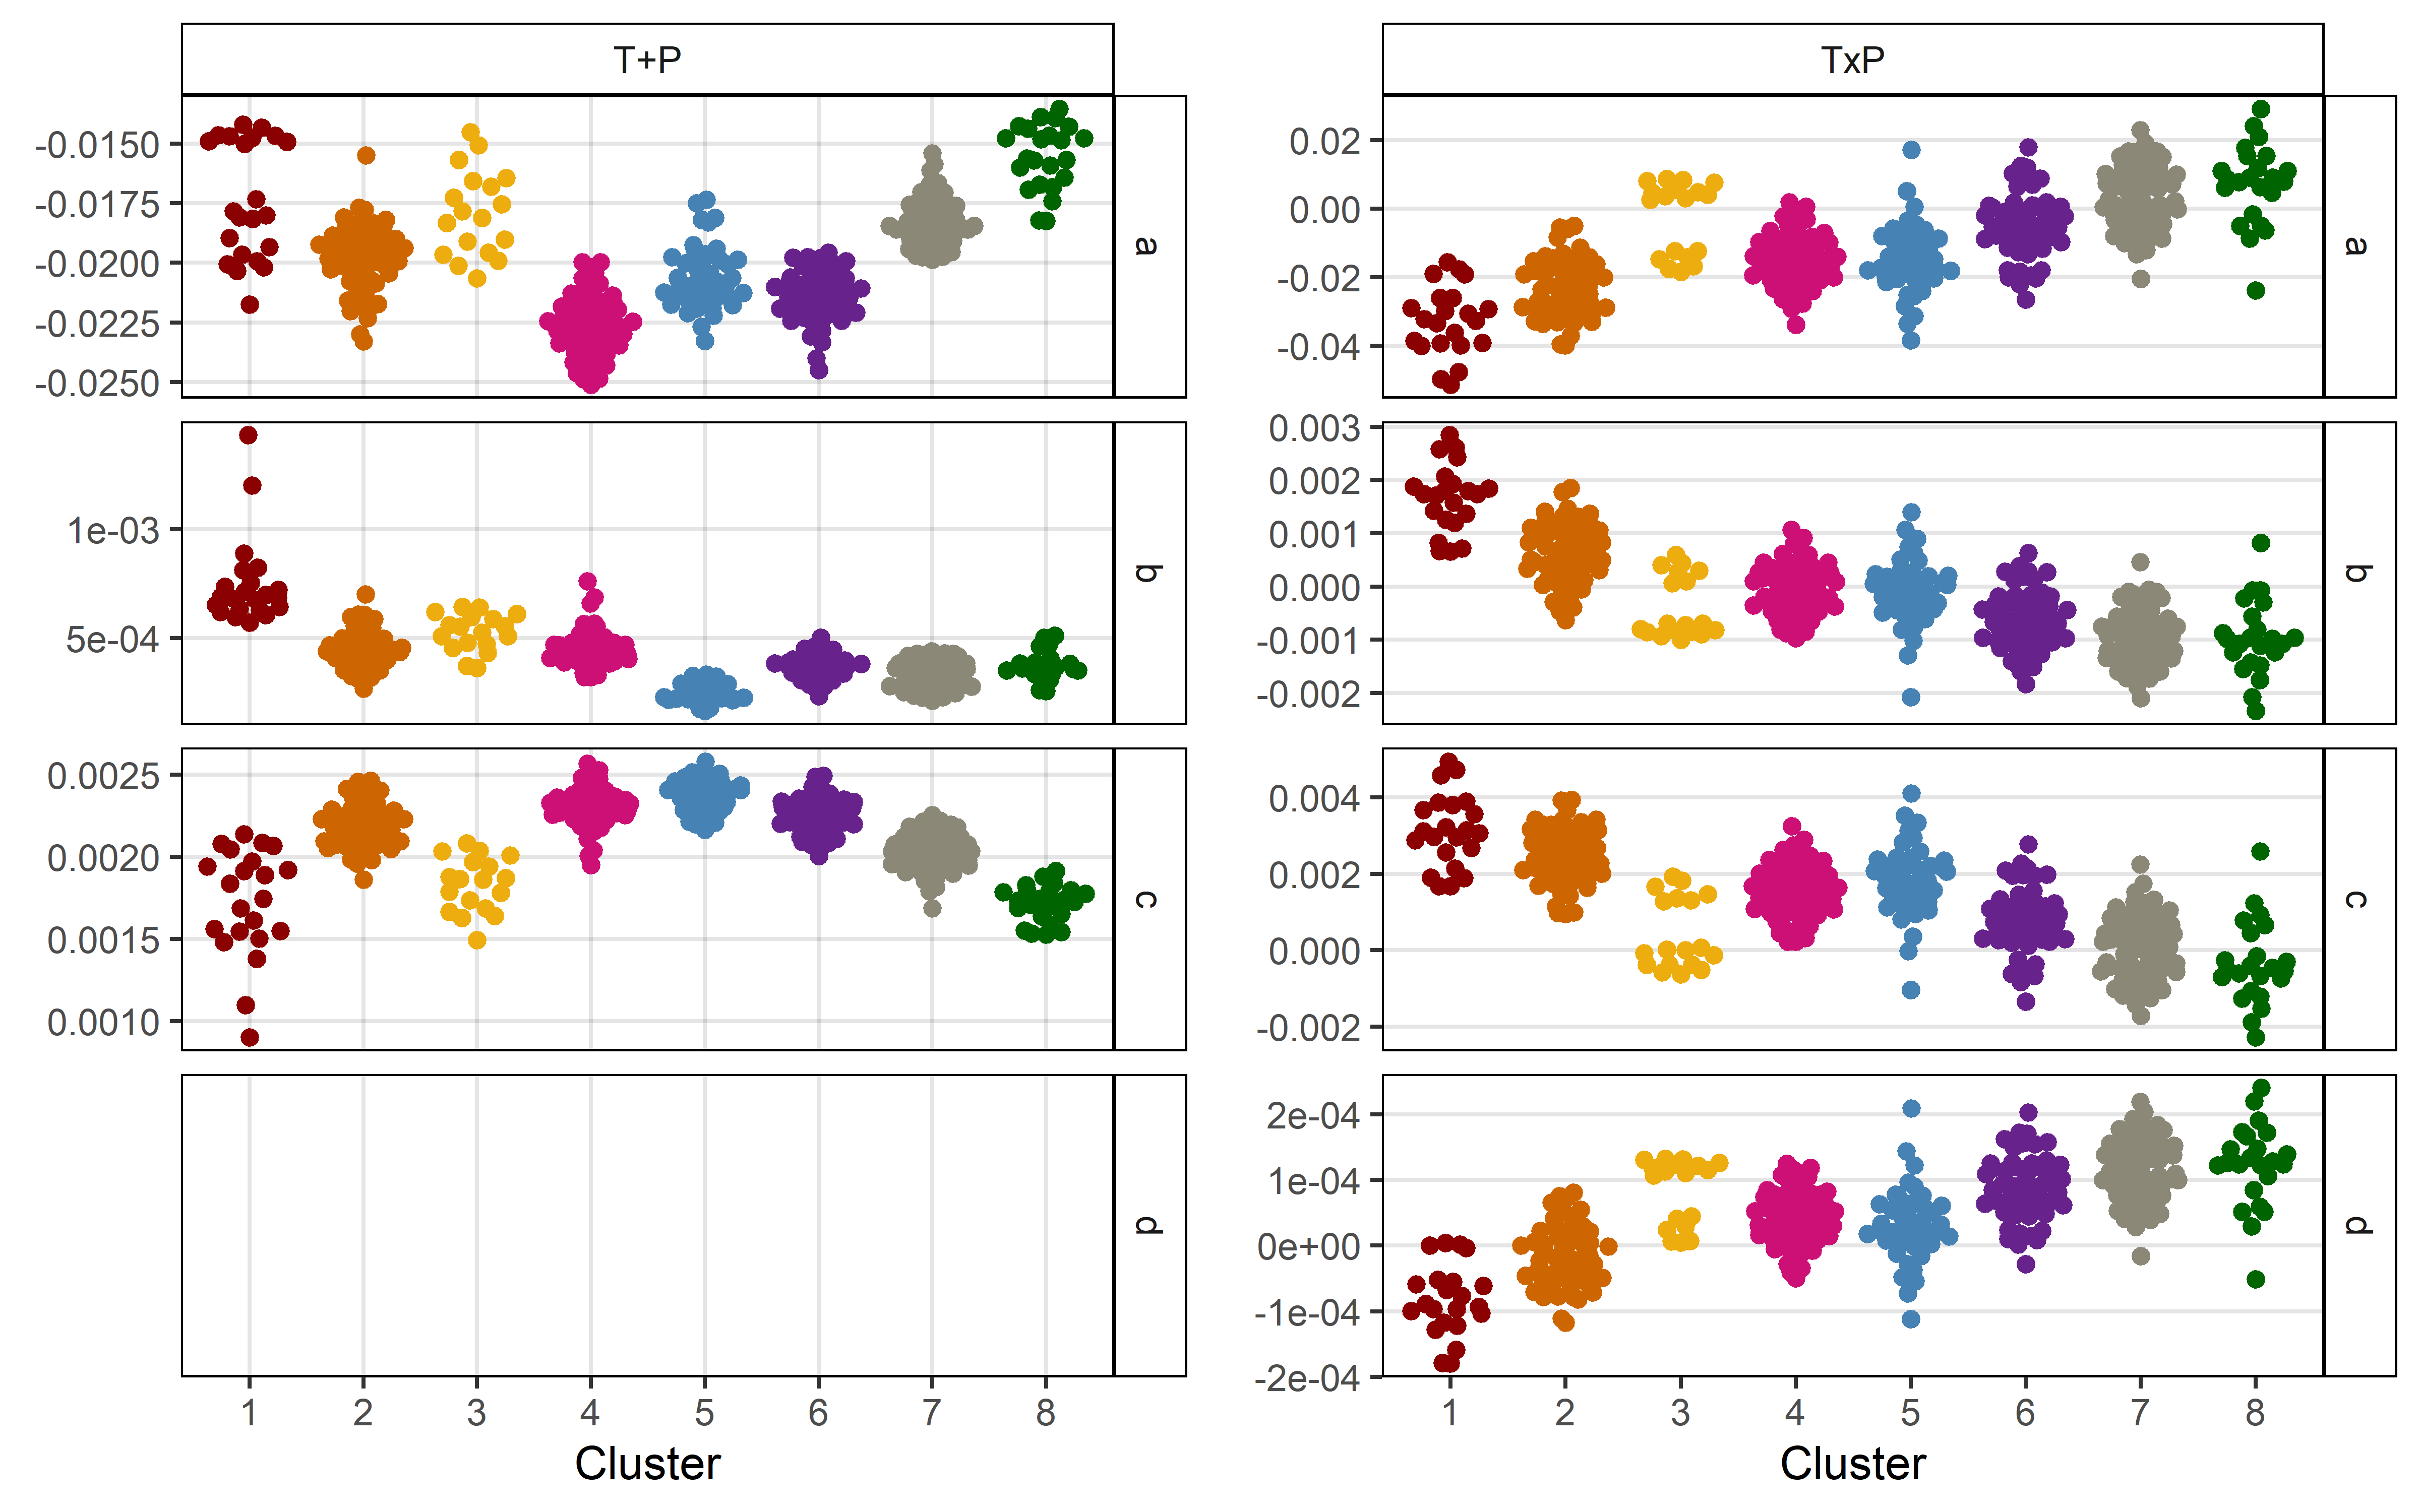
\includegraphics{Additional/Additional_Figure_11.png}

\begin{Shaded}
\begin{Highlighting}[]
\CommentTok{# Prep data}
\NormalTok{pca <-}\StringTok{ }\KeywordTok{read.csv}\NormalTok{(}\StringTok{"data/data_pca_results.csv"}\NormalTok{) }\OperatorTok\StringTok{ }\KeywordTok{mutate}\NormalTok{(}\DataTypeTok{Cluster =} \KeywordTok{factor}\NormalTok{(Cluster))}
\NormalTok{x1 <-}\StringTok{ }\KeywordTok{read.csv}\NormalTok{(}\StringTok{"data/model_t+p_coefs.csv"}\NormalTok{) }\OperatorTok\StringTok{ }\KeywordTok{mutate}\NormalTok{(}\DataTypeTok{Model =} \StringTok{"T+P"}\NormalTok{)}
\NormalTok{x2 <-}\StringTok{ }\KeywordTok{read.csv}\NormalTok{(}\StringTok{"data/model_txp_coefs.csv"}\NormalTok{) }\OperatorTok\StringTok{ }\KeywordTok{mutate}\NormalTok{(}\DataTypeTok{Model =} \StringTok{"TxP"}\NormalTok{)}
\NormalTok{xx <-}\StringTok{ }\KeywordTok{bind_rows}\NormalTok{(x1, x2) }\OperatorTok\StringTok{ }
\StringTok{  }\KeywordTok{gather}\NormalTok{(Coef, Value, a,b,c,d) }\OperatorTok
\StringTok{  }\KeywordTok{left_join}\NormalTok{(pca, }\DataTypeTok{by =} \StringTok{"Entry"}\NormalTok{) }\OperatorTok\StringTok{ }\KeywordTok{mutate}\NormalTok{(}\DataTypeTok{Cluster =} \KeywordTok{factor}\NormalTok{(Cluster))}
\CommentTok{# Plot}
\NormalTok{mp1 <-}\StringTok{ }\KeywordTok{ggplot}\NormalTok{(xx}\OperatorTok\KeywordTok{filter}\NormalTok{(Model}\OperatorTok{==}\StringTok{"T+P"}\NormalTok{), }\KeywordTok{aes}\NormalTok{(}\DataTypeTok{x =}\NormalTok{ Cluster, }\DataTypeTok{y =}\NormalTok{ Value, }\DataTypeTok{color =}\NormalTok{ Cluster)) }\OperatorTok{+}\StringTok{ }
\StringTok{  }\KeywordTok{geom_quasirandom}\NormalTok{() }\OperatorTok{+}\StringTok{ }\NormalTok{theme_AGL }\OperatorTok{+}
\StringTok{  }\KeywordTok{facet_grid}\NormalTok{(Coef}\OperatorTok{~}\NormalTok{Model, }\DataTypeTok{scales =} \StringTok{"free_y"}\NormalTok{) }\OperatorTok{+}\StringTok{ }
\StringTok{  }\KeywordTok{scale_color_manual}\NormalTok{(}\DataTypeTok{values =}\NormalTok{ colors) }\OperatorTok{+}\StringTok{ }\KeywordTok{labs}\NormalTok{(}\DataTypeTok{y =} \OtherTok{NULL}\NormalTok{)}
\NormalTok{mp2 <-}\StringTok{ }\KeywordTok{ggplot}\NormalTok{(xx}\OperatorTok\KeywordTok{filter}\NormalTok{(Model}\OperatorTok{==}\StringTok{"TxP"}\NormalTok{), }\KeywordTok{aes}\NormalTok{(}\DataTypeTok{x =}\NormalTok{ Cluster, }\DataTypeTok{y =}\NormalTok{ Value, }\DataTypeTok{color =}\NormalTok{ Cluster)) }\OperatorTok{+}\StringTok{ }
\StringTok{  }\KeywordTok{geom_quasirandom}\NormalTok{() }\OperatorTok{+}\StringTok{ }
\StringTok{  }\KeywordTok{facet_grid}\NormalTok{(Coef}\OperatorTok{~}\NormalTok{Model, }\DataTypeTok{scales =} \StringTok{"free_y"}\NormalTok{) }\OperatorTok{+}\StringTok{ }
\StringTok{  }\NormalTok{theme_AGL }\OperatorTok{+}
\StringTok{  }\KeywordTok{theme}\NormalTok{(}\DataTypeTok{panel.grid.major.x =} \KeywordTok{element_blank}\NormalTok{()) }\OperatorTok{+}
\StringTok{  }\KeywordTok{scale_color_manual}\NormalTok{(}\DataTypeTok{values =}\NormalTok{ colors) }\OperatorTok{+}\StringTok{ }\KeywordTok{labs}\NormalTok{(}\DataTypeTok{y =} \OtherTok{NULL}\NormalTok{)}
\NormalTok{mp <-}\StringTok{ }\KeywordTok{ggarrange}\NormalTok{(mp1, mp2, }\DataTypeTok{ncol =} \DecValTok{2}\NormalTok{, }\DataTypeTok{legend =} \StringTok{"none"}\NormalTok{)}
\KeywordTok{ggsave}\NormalTok{(}\StringTok{"Additional/Additional_Figure_11.png"}\NormalTok{, mp, }\DataTypeTok{width =} \DecValTok{8}\NormalTok{, }\DataTypeTok{height =} \DecValTok{5}\NormalTok{, }\DataTypeTok{dpi =} \DecValTok{600}\NormalTok{)}
\end{Highlighting}
\end{Shaded}

\hypertarget{additional-figure-12-coefficient-p-values}{%
\subsection{Additional Figure 12 Coefficient
p-values}\label{additional-figure-12-coefficient-p-values}}

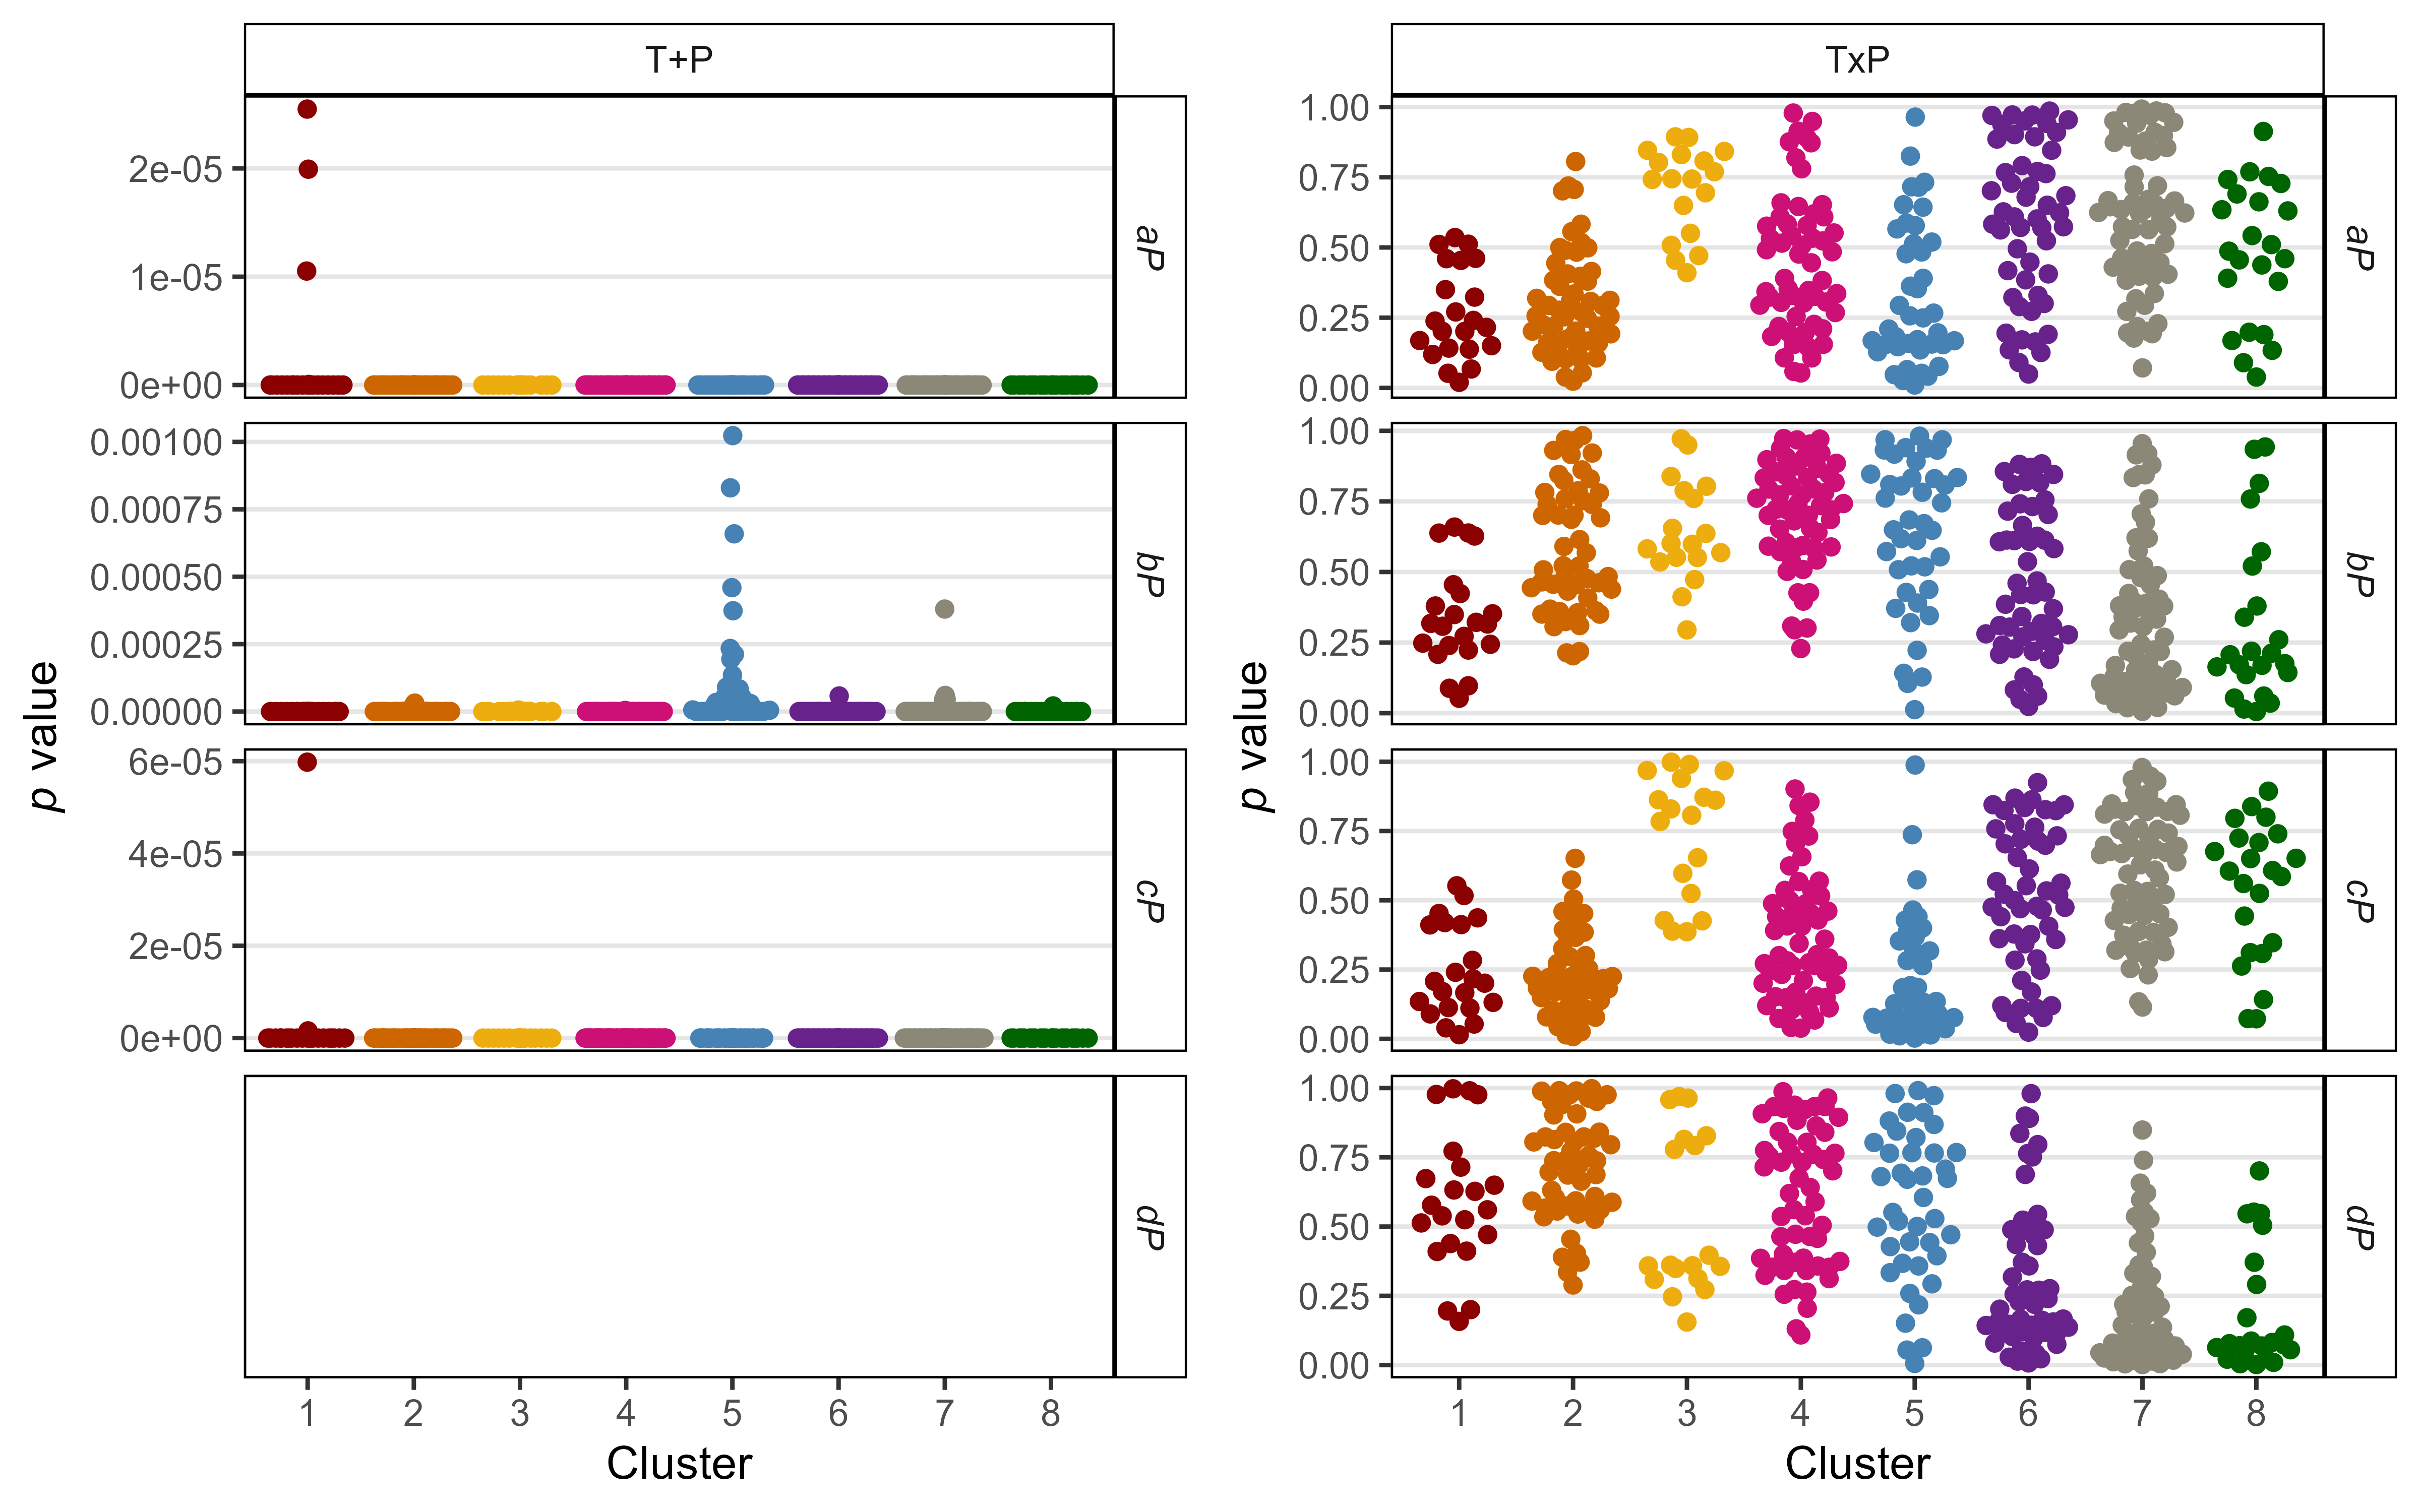
\includegraphics{Additional/Additional_Figure_12.png}

\begin{Shaded}
\begin{Highlighting}[]
\CommentTok{# Prep data}
\NormalTok{pca <-}\StringTok{ }\KeywordTok{read.csv}\NormalTok{(}\StringTok{"data/data_pca_results.csv"}\NormalTok{) }\OperatorTok\StringTok{ }\KeywordTok{mutate}\NormalTok{(}\DataTypeTok{Cluster =} \KeywordTok{factor}\NormalTok{(Cluster))}
\NormalTok{x1 <-}\StringTok{ }\KeywordTok{read.csv}\NormalTok{(}\StringTok{"data/model_t+p_coefs.csv"}\NormalTok{) }\OperatorTok\StringTok{ }\KeywordTok{mutate}\NormalTok{(}\DataTypeTok{Model =} \StringTok{"T+P"}\NormalTok{)}
\NormalTok{x2 <-}\StringTok{ }\KeywordTok{read.csv}\NormalTok{(}\StringTok{"data/model_txp_coefs.csv"}\NormalTok{) }\OperatorTok\StringTok{ }\KeywordTok{mutate}\NormalTok{(}\DataTypeTok{Model =} \StringTok{"TxP"}\NormalTok{)}
\NormalTok{xx <-}\StringTok{ }\KeywordTok{bind_rows}\NormalTok{(x1, x2) }\OperatorTok\StringTok{ }\KeywordTok{gather}\NormalTok{(Coef, Value, aP,bP,cP,dP) }\OperatorTok
\StringTok{  }\KeywordTok{left_join}\NormalTok{(pca, }\DataTypeTok{by =} \StringTok{"Entry"}\NormalTok{) }\OperatorTok\StringTok{ }\KeywordTok{mutate}\NormalTok{(}\DataTypeTok{Cluster =} \KeywordTok{factor}\NormalTok{(Cluster))}
\CommentTok{# Plot}
\NormalTok{mp1 <-}\StringTok{ }\KeywordTok{ggplot}\NormalTok{(xx}\OperatorTok\KeywordTok{filter}\NormalTok{(Model}\OperatorTok{==}\StringTok{"T+P"}\NormalTok{), }\KeywordTok{aes}\NormalTok{(}\DataTypeTok{x =}\NormalTok{ Cluster, }\DataTypeTok{y =}\NormalTok{ Value, }\DataTypeTok{color =}\NormalTok{ Cluster)) }\OperatorTok{+}\StringTok{ }
\StringTok{  }\KeywordTok{geom_quasirandom}\NormalTok{() }\OperatorTok{+}\StringTok{ }
\StringTok{  }\KeywordTok{facet_grid}\NormalTok{(Coef}\OperatorTok{~}\NormalTok{Model, }\DataTypeTok{scales =} \StringTok{"free_y"}\NormalTok{) }\OperatorTok{+}\StringTok{ }
\StringTok{  }\KeywordTok{scale_color_manual}\NormalTok{(}\DataTypeTok{values =}\NormalTok{ colors) }\OperatorTok{+}
\StringTok{  }\NormalTok{theme_AGL }\OperatorTok{+}
\StringTok{  }\KeywordTok{theme}\NormalTok{(}\DataTypeTok{panel.grid.major.x =} \KeywordTok{element_blank}\NormalTok{())  }\OperatorTok{+}
\StringTok{  }\KeywordTok{labs}\NormalTok{(}\DataTypeTok{y =} \StringTok{"p value"}\NormalTok{)}
\NormalTok{mp2 <-}\StringTok{ }\KeywordTok{ggplot}\NormalTok{(xx}\OperatorTok\KeywordTok{filter}\NormalTok{(Model}\OperatorTok{==}\StringTok{"TxP"}\NormalTok{), }\KeywordTok{aes}\NormalTok{(}\DataTypeTok{x =}\NormalTok{ Cluster, }\DataTypeTok{y =}\NormalTok{ Value, }\DataTypeTok{color =}\NormalTok{ Cluster)) }\OperatorTok{+}\StringTok{ }
\StringTok{  }\KeywordTok{geom_quasirandom}\NormalTok{() }\OperatorTok{+}\StringTok{ }
\StringTok{  }\KeywordTok{facet_grid}\NormalTok{(Coef }\OperatorTok{~}\StringTok{ }\NormalTok{Model, }\DataTypeTok{scales =} \StringTok{"free_y"}\NormalTok{) }\OperatorTok{+}\StringTok{ }
\StringTok{  }\NormalTok{theme_AGL }\OperatorTok{+}
\StringTok{  }\KeywordTok{theme}\NormalTok{(}\DataTypeTok{panel.grid.major.x =} \KeywordTok{element_blank}\NormalTok{()) }\OperatorTok{+}
\StringTok{  }\KeywordTok{scale_color_manual}\NormalTok{(}\DataTypeTok{values =}\NormalTok{ colors) }\OperatorTok{+}
\StringTok{  }\KeywordTok{labs}\NormalTok{(}\DataTypeTok{y =} \StringTok{"p value"}\NormalTok{)}
\NormalTok{mp <-}\StringTok{ }\KeywordTok{ggarrange}\NormalTok{(mp1,mp2,}\DataTypeTok{ncol=}\DecValTok{2}\NormalTok{, }\DataTypeTok{legend =} \StringTok{"none"}\NormalTok{) }
\KeywordTok{ggsave}\NormalTok{(}\StringTok{"Additional/Additional_Figure_12.png"}\NormalTok{, mp, }\DataTypeTok{width =} \DecValTok{8}\NormalTok{, }\DataTypeTok{height =} \DecValTok{5}\NormalTok{, }\DataTypeTok{dpi =} \DecValTok{600}\NormalTok{)}
\end{Highlighting}
\end{Shaded}

\hypertarget{additional-figure-13-p-values-b-c}{%
\subsection{Additional Figure 13 p-values b
c}\label{additional-figure-13-p-values-b-c}}

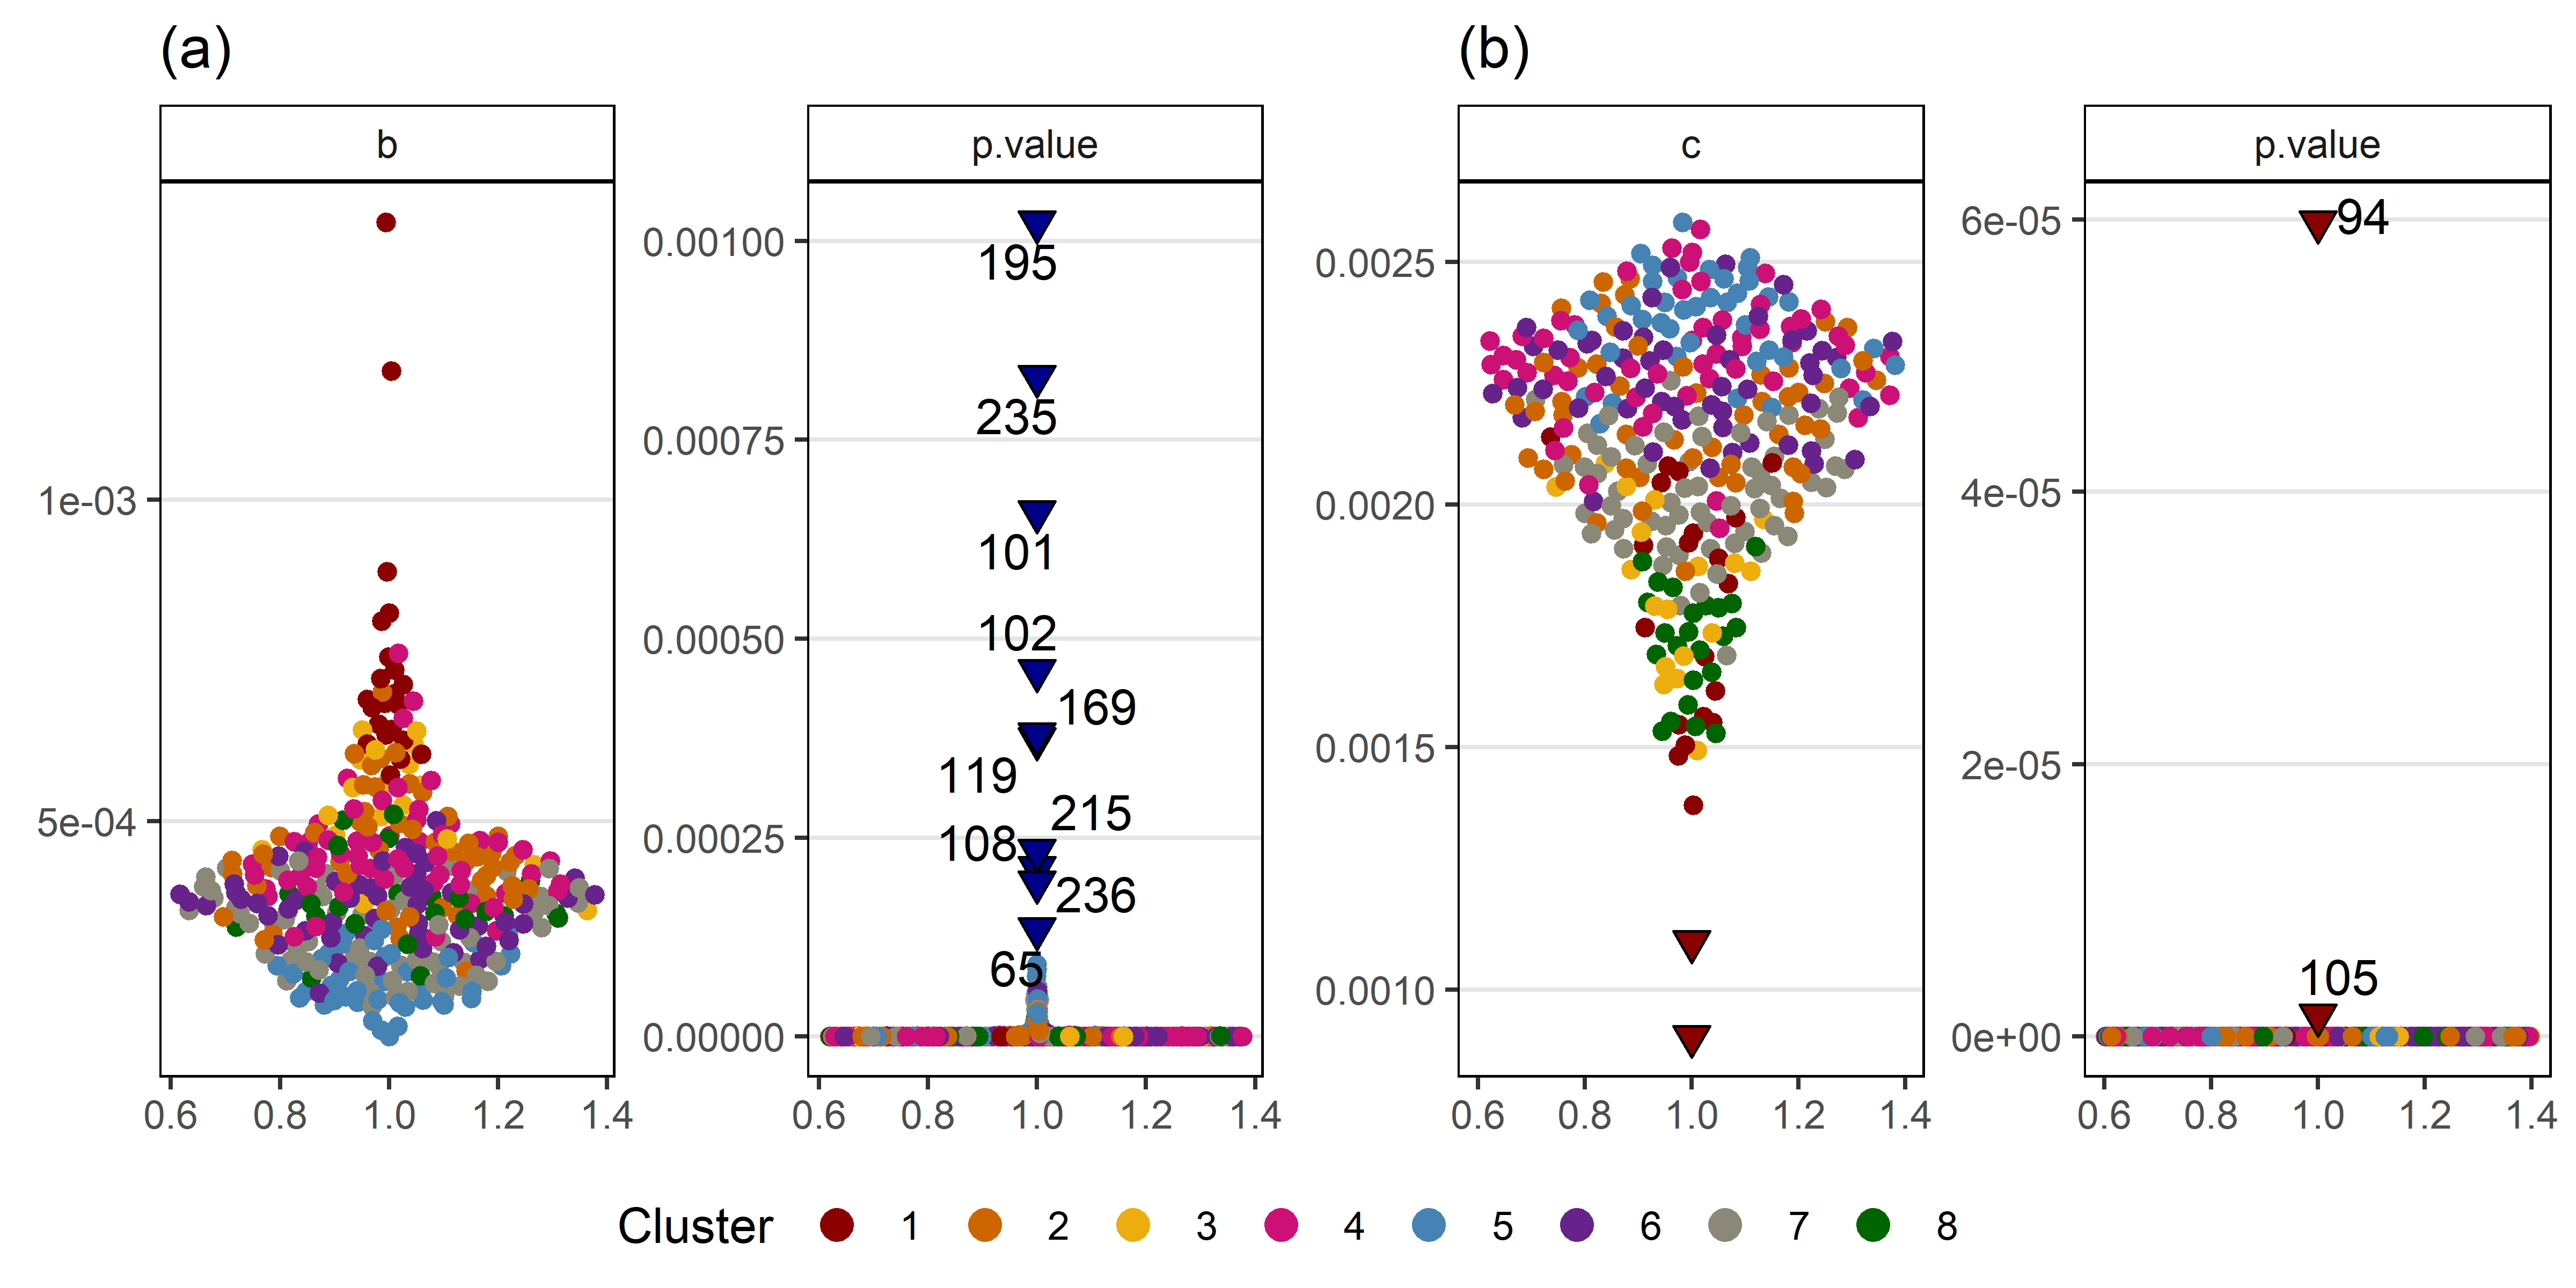
\includegraphics{Additional/Additional_Figure_13.png}

\begin{Shaded}
\begin{Highlighting}[]
\CommentTok{# Prep data}
\NormalTok{pca <-}\StringTok{ }\KeywordTok{read.csv}\NormalTok{(}\StringTok{"data/data_pca_results.csv"}\NormalTok{) }\OperatorTok\StringTok{ }\KeywordTok{mutate}\NormalTok{(}\DataTypeTok{Cluster =} \KeywordTok{factor}\NormalTok{(Cluster))}
\NormalTok{xx <-}\StringTok{ }\KeywordTok{read.csv}\NormalTok{(}\StringTok{"data/model_t+p_coefs.csv"}\NormalTok{) }\OperatorTok\StringTok{ }
\StringTok{  }\KeywordTok{mutate}\NormalTok{(}\DataTypeTok{Sig =} \KeywordTok{factor}\NormalTok{(}\KeywordTok{ifelse}\NormalTok{(bP }\OperatorTok{>}\StringTok{ }\FloatTok{0.0001}\NormalTok{, }\StringTok{"Sig"}\NormalTok{,}\StringTok{"Less Sig"}\NormalTok{))) }\OperatorTok
\StringTok{  }\KeywordTok{select}\NormalTok{(Entry, Sig, }\DataTypeTok{p.value=}\NormalTok{bP, b) }\OperatorTok\StringTok{ }
\StringTok{  }\KeywordTok{gather}\NormalTok{(Trait, Value, p.value, b) }\OperatorTok
\StringTok{  }\KeywordTok{left_join}\NormalTok{(pca, }\DataTypeTok{by =} \StringTok{"Entry"}\NormalTok{)}
\NormalTok{x1 <-}\StringTok{ }\NormalTok{xx }\OperatorTok\StringTok{ }\KeywordTok{filter}\NormalTok{(Sig }\OperatorTok{==}\StringTok{ "Sig"}\NormalTok{, Trait }\OperatorTok{==}\StringTok{ "p.value"}\NormalTok{)}
\CommentTok{# Plot (a)}
\NormalTok{mp1 <-}\StringTok{ }\KeywordTok{ggplot}\NormalTok{(xx, }\KeywordTok{aes}\NormalTok{(}\DataTypeTok{x =} \DecValTok{1}\NormalTok{, }\DataTypeTok{y =}\NormalTok{ Value)) }\OperatorTok{+}
\StringTok{  }\KeywordTok{geom_quasirandom}\NormalTok{(}\KeywordTok{aes}\NormalTok{(}\DataTypeTok{color =}\NormalTok{ Cluster)) }\OperatorTok{+}
\StringTok{    }\KeywordTok{geom_point}\NormalTok{(}\DataTypeTok{data =}\NormalTok{ x1, }\DataTypeTok{size =} \FloatTok{2.5}\NormalTok{, }\DataTypeTok{pch =} \DecValTok{25}\NormalTok{, }\DataTypeTok{color =} \StringTok{"black"}\NormalTok{, }\DataTypeTok{fill =} \StringTok{"darkblue"}\NormalTok{) }\OperatorTok{+}
\StringTok{  }\KeywordTok{geom_text_repel}\NormalTok{(}\DataTypeTok{data =}\NormalTok{ x1, }\KeywordTok{aes}\NormalTok{(}\DataTypeTok{label =}\NormalTok{ Entry)) }\OperatorTok{+}
\StringTok{  }\KeywordTok{facet_wrap}\NormalTok{(.}\OperatorTok{~}\NormalTok{Trait, }\DataTypeTok{scales =} \StringTok{"free_y"}\NormalTok{) }\OperatorTok{+}
\StringTok{  }\KeywordTok{scale_color_manual}\NormalTok{(}\DataTypeTok{values =}\NormalTok{ colors) }\OperatorTok{+}
\StringTok{  }\KeywordTok{guides}\NormalTok{(}\DataTypeTok{colour =} \KeywordTok{guide_legend}\NormalTok{(}\DataTypeTok{nrow =} \DecValTok{1}\NormalTok{, }\DataTypeTok{override.aes =} \KeywordTok{list}\NormalTok{(}\DataTypeTok{size =} \DecValTok{3}\NormalTok{))) }\OperatorTok{+}
\StringTok{  }\NormalTok{theme_AGL }\OperatorTok{+}
\StringTok{  }\KeywordTok{theme}\NormalTok{(}\DataTypeTok{panel.grid.major.x =} \KeywordTok{element_blank}\NormalTok{()) }\OperatorTok{+}
\StringTok{  }\KeywordTok{labs}\NormalTok{(}\DataTypeTok{title =} \StringTok{"(a)"}\NormalTok{, }\DataTypeTok{x =} \OtherTok{NULL}\NormalTok{, }\DataTypeTok{y =} \OtherTok{NULL}\NormalTok{)}
\CommentTok{# Prep data}
\NormalTok{xx <-}\StringTok{ }\KeywordTok{read.csv}\NormalTok{(}\StringTok{"data/model_t+p_coefs.csv"}\NormalTok{) }\OperatorTok\StringTok{ }
\StringTok{  }\KeywordTok{mutate}\NormalTok{(}\DataTypeTok{Sig =} \KeywordTok{factor}\NormalTok{(}\KeywordTok{ifelse}\NormalTok{(cP }\OperatorTok{>}\StringTok{ }\FloatTok{0.000001}\NormalTok{, }\StringTok{"Sig"}\NormalTok{,}\StringTok{"Less Sig"}\NormalTok{))) }\OperatorTok
\StringTok{  }\KeywordTok{select}\NormalTok{(Entry, Sig, }\DataTypeTok{p.value=}\NormalTok{cP, c) }\OperatorTok\StringTok{ }
\StringTok{  }\KeywordTok{gather}\NormalTok{(Trait, Value, p.value, c) }\OperatorTok
\StringTok{  }\KeywordTok{left_join}\NormalTok{(pca, }\DataTypeTok{by =} \StringTok{"Entry"}\NormalTok{)}
\NormalTok{x1 <-}\StringTok{ }\NormalTok{xx }\OperatorTok\StringTok{ }\KeywordTok{filter}\NormalTok{(Sig }\OperatorTok{==}\StringTok{ "Sig"}\NormalTok{)}
\CommentTok{# Plot B)}
\NormalTok{mp2 <-}\StringTok{ }\KeywordTok{ggplot}\NormalTok{(xx, }\KeywordTok{aes}\NormalTok{(}\DataTypeTok{x =} \DecValTok{1}\NormalTok{, }\DataTypeTok{y =}\NormalTok{ Value)) }\OperatorTok{+}
\StringTok{  }\KeywordTok{geom_quasirandom}\NormalTok{(}\KeywordTok{aes}\NormalTok{(}\DataTypeTok{color =}\NormalTok{ Cluster)) }\OperatorTok{+}
\StringTok{  }\KeywordTok{geom_point}\NormalTok{(}\DataTypeTok{data =}\NormalTok{ x1, }\DataTypeTok{size =} \FloatTok{2.5}\NormalTok{, }\DataTypeTok{pch =} \DecValTok{25}\NormalTok{, }\DataTypeTok{color =} \StringTok{"black"}\NormalTok{, }\DataTypeTok{fill =} \StringTok{"darkred"}\NormalTok{) }\OperatorTok{+}
\StringTok{  }\KeywordTok{geom_text_repel}\NormalTok{(}\DataTypeTok{data =}\NormalTok{ x1 }\OperatorTok\StringTok{ }\KeywordTok{filter}\NormalTok{(Trait }\OperatorTok{==}\StringTok{"p.value"}\NormalTok{), }\KeywordTok{aes}\NormalTok{(}\DataTypeTok{label =}\NormalTok{ Entry)) }\OperatorTok{+}
\StringTok{  }\KeywordTok{facet_wrap}\NormalTok{(.}\OperatorTok{~}\NormalTok{Trait, }\DataTypeTok{scales =} \StringTok{"free_y"}\NormalTok{) }\OperatorTok{+}
\StringTok{  }\KeywordTok{scale_color_manual}\NormalTok{(}\DataTypeTok{values =}\NormalTok{ colors) }\OperatorTok{+}
\StringTok{  }\KeywordTok{guides}\NormalTok{(}\DataTypeTok{colour =} \KeywordTok{guide_legend}\NormalTok{(}\DataTypeTok{nrow =} \DecValTok{1}\NormalTok{, }\DataTypeTok{override.aes =} \KeywordTok{list}\NormalTok{(}\DataTypeTok{size =} \DecValTok{3}\NormalTok{))) }\OperatorTok{+}
\StringTok{  }\NormalTok{theme_AGL }\OperatorTok{+}
\StringTok{  }\KeywordTok{theme}\NormalTok{(}\DataTypeTok{panel.grid.major.x =} \KeywordTok{element_blank}\NormalTok{()) }\OperatorTok{+}
\StringTok{  }\KeywordTok{labs}\NormalTok{(}\DataTypeTok{title =} \StringTok{"(b)"}\NormalTok{, }\DataTypeTok{x =} \OtherTok{NULL}\NormalTok{, }\DataTypeTok{y =} \OtherTok{NULL}\NormalTok{)}
\CommentTok{# Append (a) and (b)}
\NormalTok{mp <-}\StringTok{ }\KeywordTok{ggarrange}\NormalTok{(mp1, mp2, }\DataTypeTok{ncol =} \DecValTok{2}\NormalTok{, }\DataTypeTok{common.legend =}\NormalTok{ T, }\DataTypeTok{legend =} \StringTok{"bottom"}\NormalTok{)}
\KeywordTok{ggsave}\NormalTok{(}\StringTok{"Additional/Additional_Figure_13.png"}\NormalTok{, mp, }\DataTypeTok{width =} \DecValTok{8}\NormalTok{, }\DataTypeTok{height =} \DecValTok{4}\NormalTok{, }\DataTypeTok{dpi =} \DecValTok{600}\NormalTok{)}
\end{Highlighting}
\end{Shaded}

\hypertarget{modeling-dtf-t-p---location-out}{%
\subsection{Modeling DTF (T + P) - Location
Out}\label{modeling-dtf-t-p---location-out}}

Train the model without the location used for prediction

\begin{Shaded}
\begin{Highlighting}[]
\CommentTok{####################################}
\CommentTok{# 1/f = a + bT + cP (Location Out) #}
\CommentTok{####################################}
\CommentTok{# Prep data}
\NormalTok{xx <-}\StringTok{ }\NormalTok{rr }\OperatorTok\StringTok{ }\KeywordTok{filter}\NormalTok{(}\OperatorTok{!}\KeywordTok{is.na}\NormalTok{(RDTF)) }\OperatorTok
\StringTok{  }\KeywordTok{left_join}\NormalTok{(}\KeywordTok{select}\NormalTok{(ff, Expt, T_mean, P_mean), }\DataTypeTok{by =} \StringTok{"Expt"}\NormalTok{)}
\NormalTok{mr <-}\StringTok{ }\OtherTok{NULL}\NormalTok{; md <-}\StringTok{ }\OtherTok{NULL}
\CommentTok{# Model - For each Location, the model is re-trained without that locations data}
\ControlFlowTok{for}\NormalTok{(i }\ControlFlowTok{in} \DecValTok{1}\OperatorTok{:}\DecValTok{324}\NormalTok{) \{}
  \ControlFlowTok{for}\NormalTok{(k }\ControlFlowTok{in} \KeywordTok{unique}\NormalTok{(xx}\OperatorTok{$}\NormalTok{Location)) \{}
    \CommentTok{# Prep data}
\NormalTok{    xi1 <-}\StringTok{ }\NormalTok{xx }\OperatorTok\StringTok{ }\KeywordTok{filter}\NormalTok{(Entry }\OperatorTok{==}\StringTok{ }\NormalTok{i, Location }\OperatorTok{!=}\StringTok{ }\NormalTok{k)}
\NormalTok{    xi2 <-}\StringTok{ }\NormalTok{xx }\OperatorTok\StringTok{ }\KeywordTok{filter}\NormalTok{(Entry }\OperatorTok{==}\StringTok{ }\NormalTok{i, Location }\OperatorTok{==}\StringTok{ }\NormalTok{k) }
\NormalTok{    xd2 <-}\StringTok{ }\NormalTok{xi2 }\OperatorTok\StringTok{ }\KeywordTok{group_by}\NormalTok{(Entry, Name, Expt, ExptShort) }\OperatorTok\StringTok{ }
\StringTok{      }\KeywordTok{summarise_at}\NormalTok{(}\KeywordTok{vars}\NormalTok{(DTF, RDTF, T_mean, P_mean), }\KeywordTok{funs}\NormalTok{(mean), }\DataTypeTok{na.rm =}\NormalTok{ T) }\OperatorTok
\StringTok{      }\KeywordTok{ungroup}\NormalTok{()}
    \CommentTok{# Train model}
\NormalTok{    mi <-}\StringTok{ }\KeywordTok{lm}\NormalTok{(RDTF }\OperatorTok{~}\StringTok{ }\NormalTok{T_mean }\OperatorTok{*}\StringTok{ }\NormalTok{P_mean, }\DataTypeTok{data =}\NormalTok{ xi1)}
    \CommentTok{# Predict DTF}
\NormalTok{    xi2 <-}\StringTok{ }\NormalTok{xi2 }\OperatorTok\StringTok{ }\KeywordTok{mutate}\NormalTok{(}\DataTypeTok{Predicted_DTF =} \DecValTok{1} \OperatorTok{/}\StringTok{ }\KeywordTok{predict}\NormalTok{(mi, }\DataTypeTok{newdata =}\NormalTok{ xi2))}
\NormalTok{    xd2 <-}\StringTok{ }\NormalTok{xd2 }\OperatorTok\StringTok{ }\KeywordTok{mutate}\NormalTok{(}\DataTypeTok{Predicted_DTF =} \DecValTok{1} \OperatorTok{/}\StringTok{ }\KeywordTok{predict}\NormalTok{(mi, }\DataTypeTok{newdata =}\NormalTok{ xd2))}
    \CommentTok{# Save to table}
\NormalTok{    mr <-}\StringTok{ }\KeywordTok{bind_rows}\NormalTok{(mr, xi2)}
\NormalTok{    md <-}\StringTok{ }\KeywordTok{bind_rows}\NormalTok{(md, xd2)}
\NormalTok{  \}}
\NormalTok{\}}
\CommentTok{# Save Results}
\KeywordTok{write.csv}\NormalTok{(mr, }\StringTok{"data/model_test.csv"}\NormalTok{, }\DataTypeTok{row.names =}\NormalTok{ F)}
\KeywordTok{write.csv}\NormalTok{(md, }\StringTok{"data/model_test_d.csv"}\NormalTok{, }\DataTypeTok{row.names =}\NormalTok{ F)}
\end{Highlighting}
\end{Shaded}

\hypertarget{figure-4-test-model}{%
\subsection{Figure 4 Test Model}\label{figure-4-test-model}}

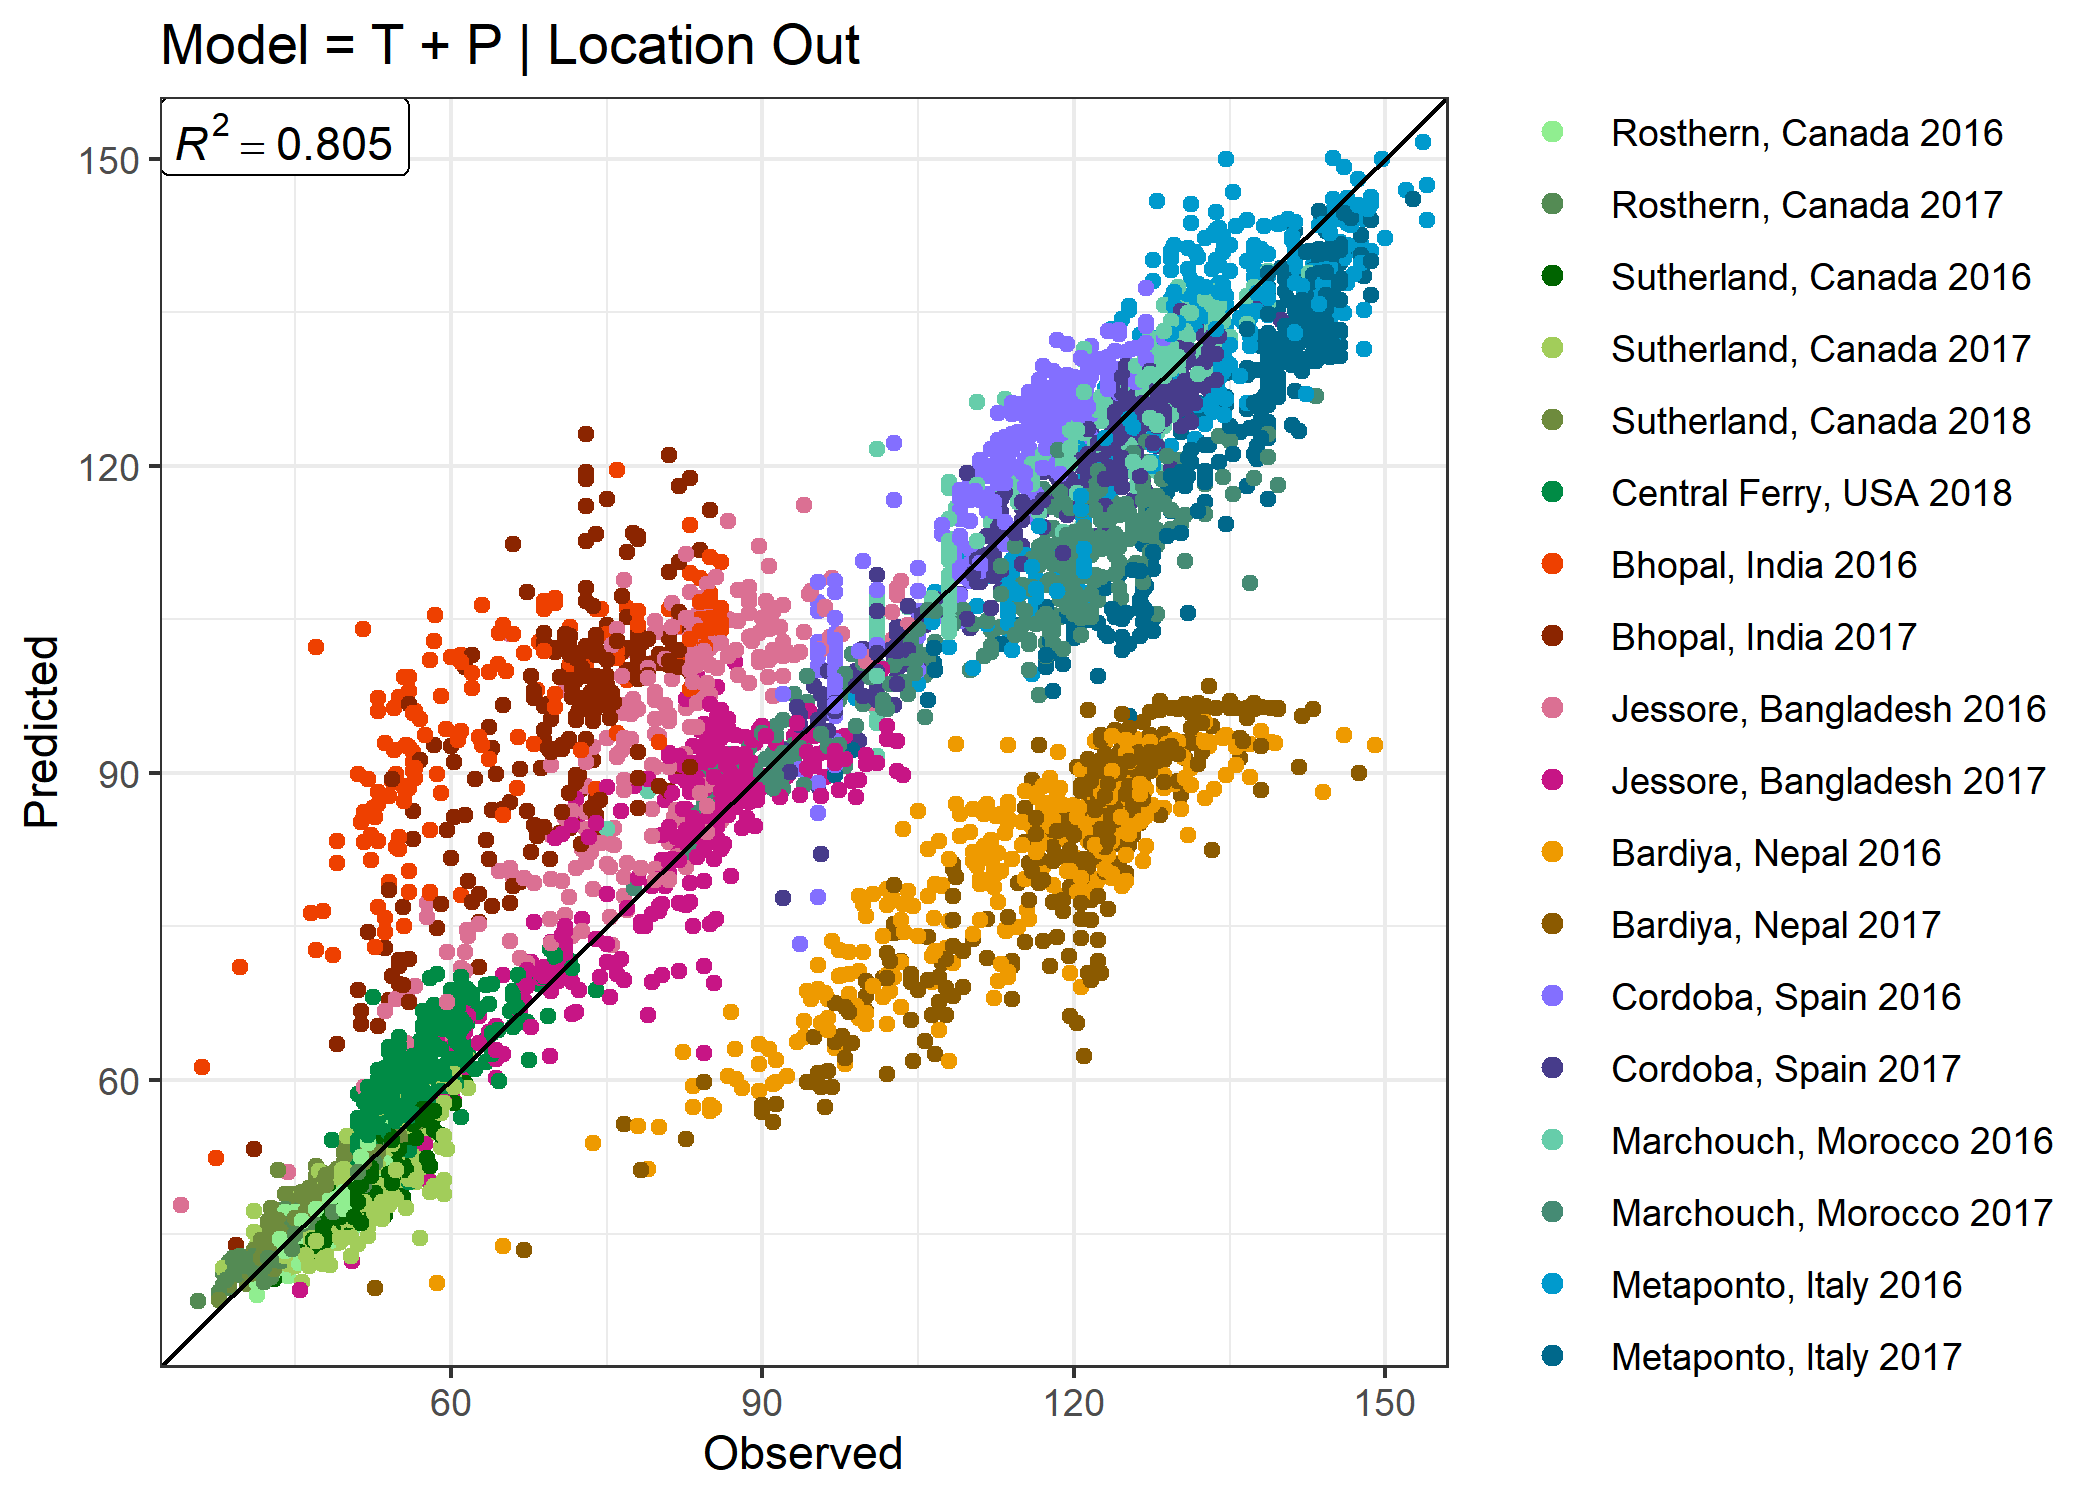
\includegraphics{Additional/Model/Model_1_3.png}

\begin{Shaded}
\begin{Highlighting}[]
\CommentTok{# Prep data}
\NormalTok{xx <-}\StringTok{ }\KeywordTok{read.csv}\NormalTok{(}\StringTok{"data/model_test_d.csv"}\NormalTok{) }\OperatorTok\StringTok{ }
\StringTok{  }\KeywordTok{mutate}\NormalTok{(}\DataTypeTok{Expt =} \KeywordTok{factor}\NormalTok{(Expt, }\DataTypeTok{levels =}\NormalTok{ names_Expt))}
\CommentTok{# Plot Observed vs Predicted}
\NormalTok{mp <-}\StringTok{ }\KeywordTok{gg_model_1}\NormalTok{(xx, }\DataTypeTok{title =} \StringTok{"Model = T + P | Location Out"}\NormalTok{)}
\KeywordTok{ggsave}\NormalTok{(}\StringTok{"Additional/Model/Model_1_3.png"}\NormalTok{, mp, }\DataTypeTok{width =} \DecValTok{7}\NormalTok{, }\DataTypeTok{height =} \DecValTok{5}\NormalTok{, }\DataTypeTok{dpi =} \DecValTok{600}\NormalTok{)}
\end{Highlighting}
\end{Shaded}

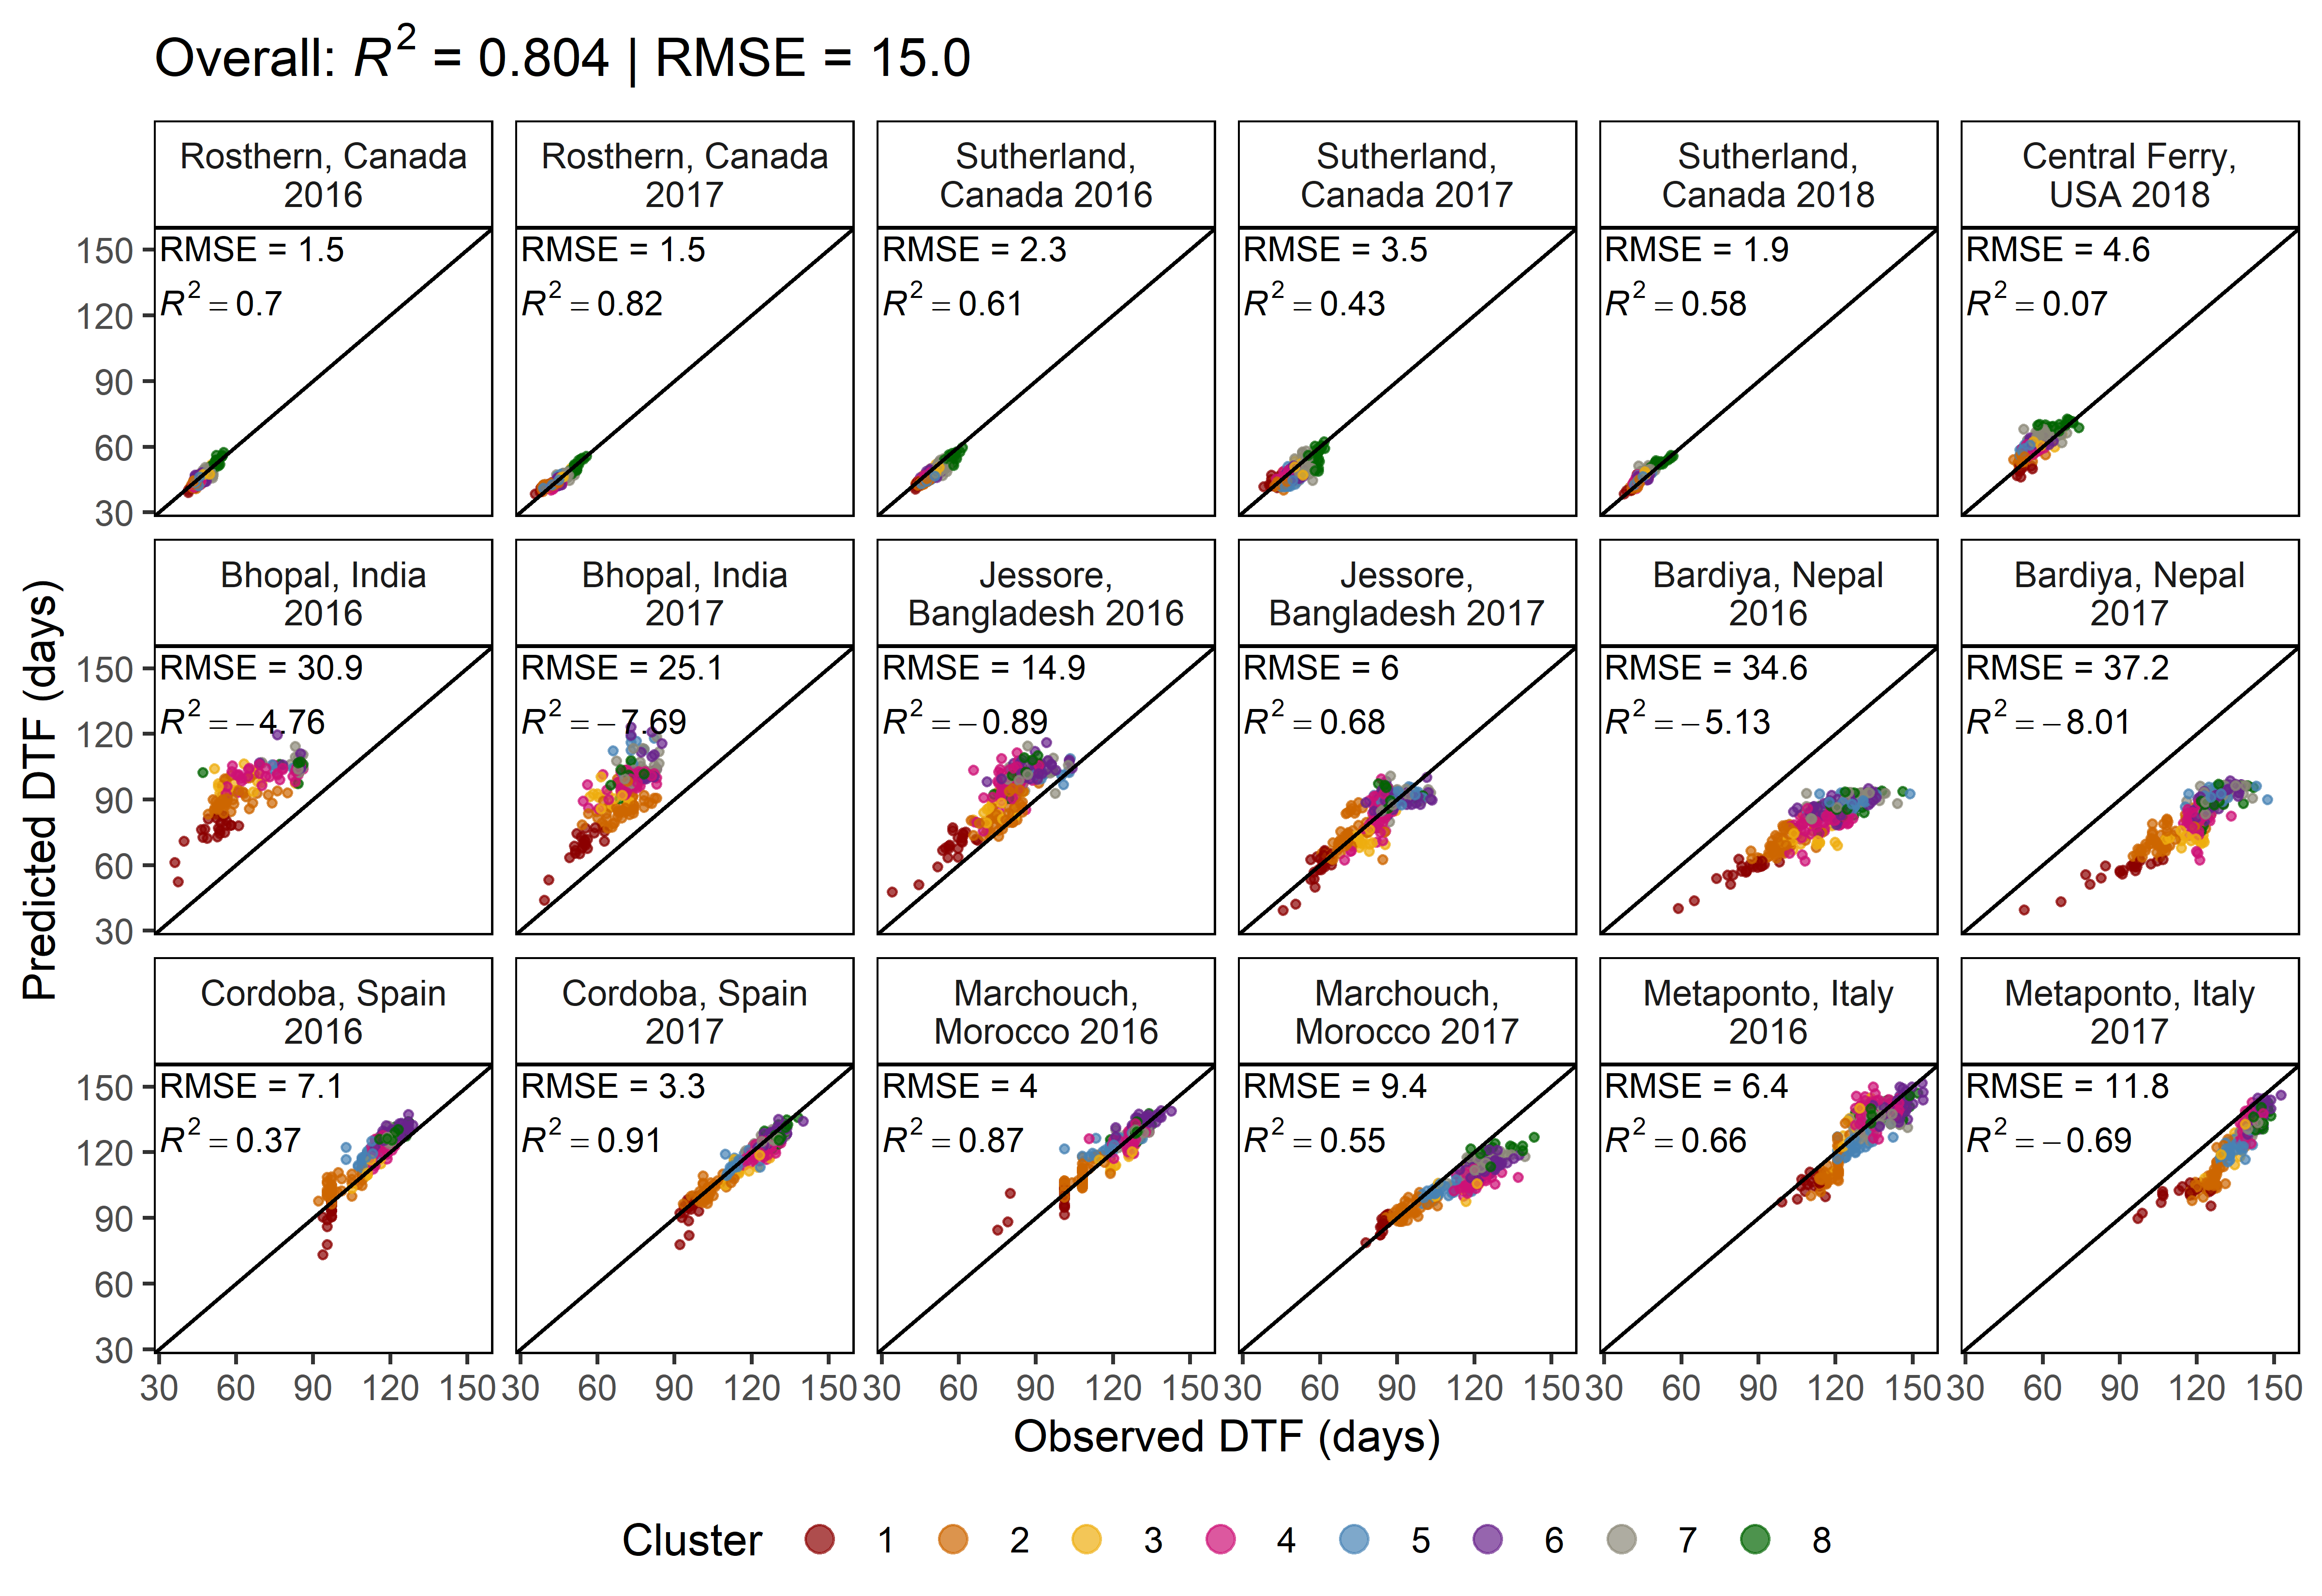
\includegraphics{Figure_04.png}

\begin{Shaded}
\begin{Highlighting}[]
\KeywordTok{modelR2}\NormalTok{(xx}\OperatorTok{$}\NormalTok{DTF, xx}\OperatorTok{$}\NormalTok{Predicted_DTF)}
\end{Highlighting}
\end{Shaded}

\begin{verbatim}
[1] 0.8045254
\end{verbatim}

\begin{Shaded}
\begin{Highlighting}[]
\KeywordTok{modelRMSE}\NormalTok{(xx}\OperatorTok{$}\NormalTok{DTF, xx}\OperatorTok{$}\NormalTok{Predicted_DTF)}
\end{Highlighting}
\end{Shaded}

\begin{verbatim}
[1] 15.01078
\end{verbatim}

\begin{Shaded}
\begin{Highlighting}[]
\CommentTok{# Plot (a)}
\NormalTok{mp <-}\StringTok{ }\KeywordTok{gg_model_2}\NormalTok{(xx, }\DataTypeTok{title =} \KeywordTok{expression}\NormalTok{(}\KeywordTok{paste}\NormalTok{(}\StringTok{"Overall: "}\NormalTok{,}
        \KeywordTok{italic}\NormalTok{(}\StringTok{"R"}\NormalTok{)}\OperatorTok{^}\DecValTok{2}\NormalTok{, }\StringTok{" = 0.804 | RMSE = 15.0"}\NormalTok{)))}
\KeywordTok{ggsave}\NormalTok{(}\StringTok{"Figure_04.png"}\NormalTok{, mp, }\DataTypeTok{width =} \DecValTok{8}\NormalTok{, }\DataTypeTok{height =} \FloatTok{5.5}\NormalTok{, }\DataTypeTok{dpi =} \DecValTok{600}\NormalTok{)}
\NormalTok{mp <-}\StringTok{ }\KeywordTok{gg_model_2}\NormalTok{(xx, }\DataTypeTok{title =} \StringTok{"Model = T + P | Location Out"}\NormalTok{)}
\KeywordTok{ggsave}\NormalTok{(}\StringTok{"Additional/Model/Model_2_3.png"}\NormalTok{, mp, }\DataTypeTok{width =} \DecValTok{8}\NormalTok{, }\DataTypeTok{height =} \FloatTok{5.5}\NormalTok{, }\DataTypeTok{dpi =} \DecValTok{600}\NormalTok{)}
\end{Highlighting}
\end{Shaded}

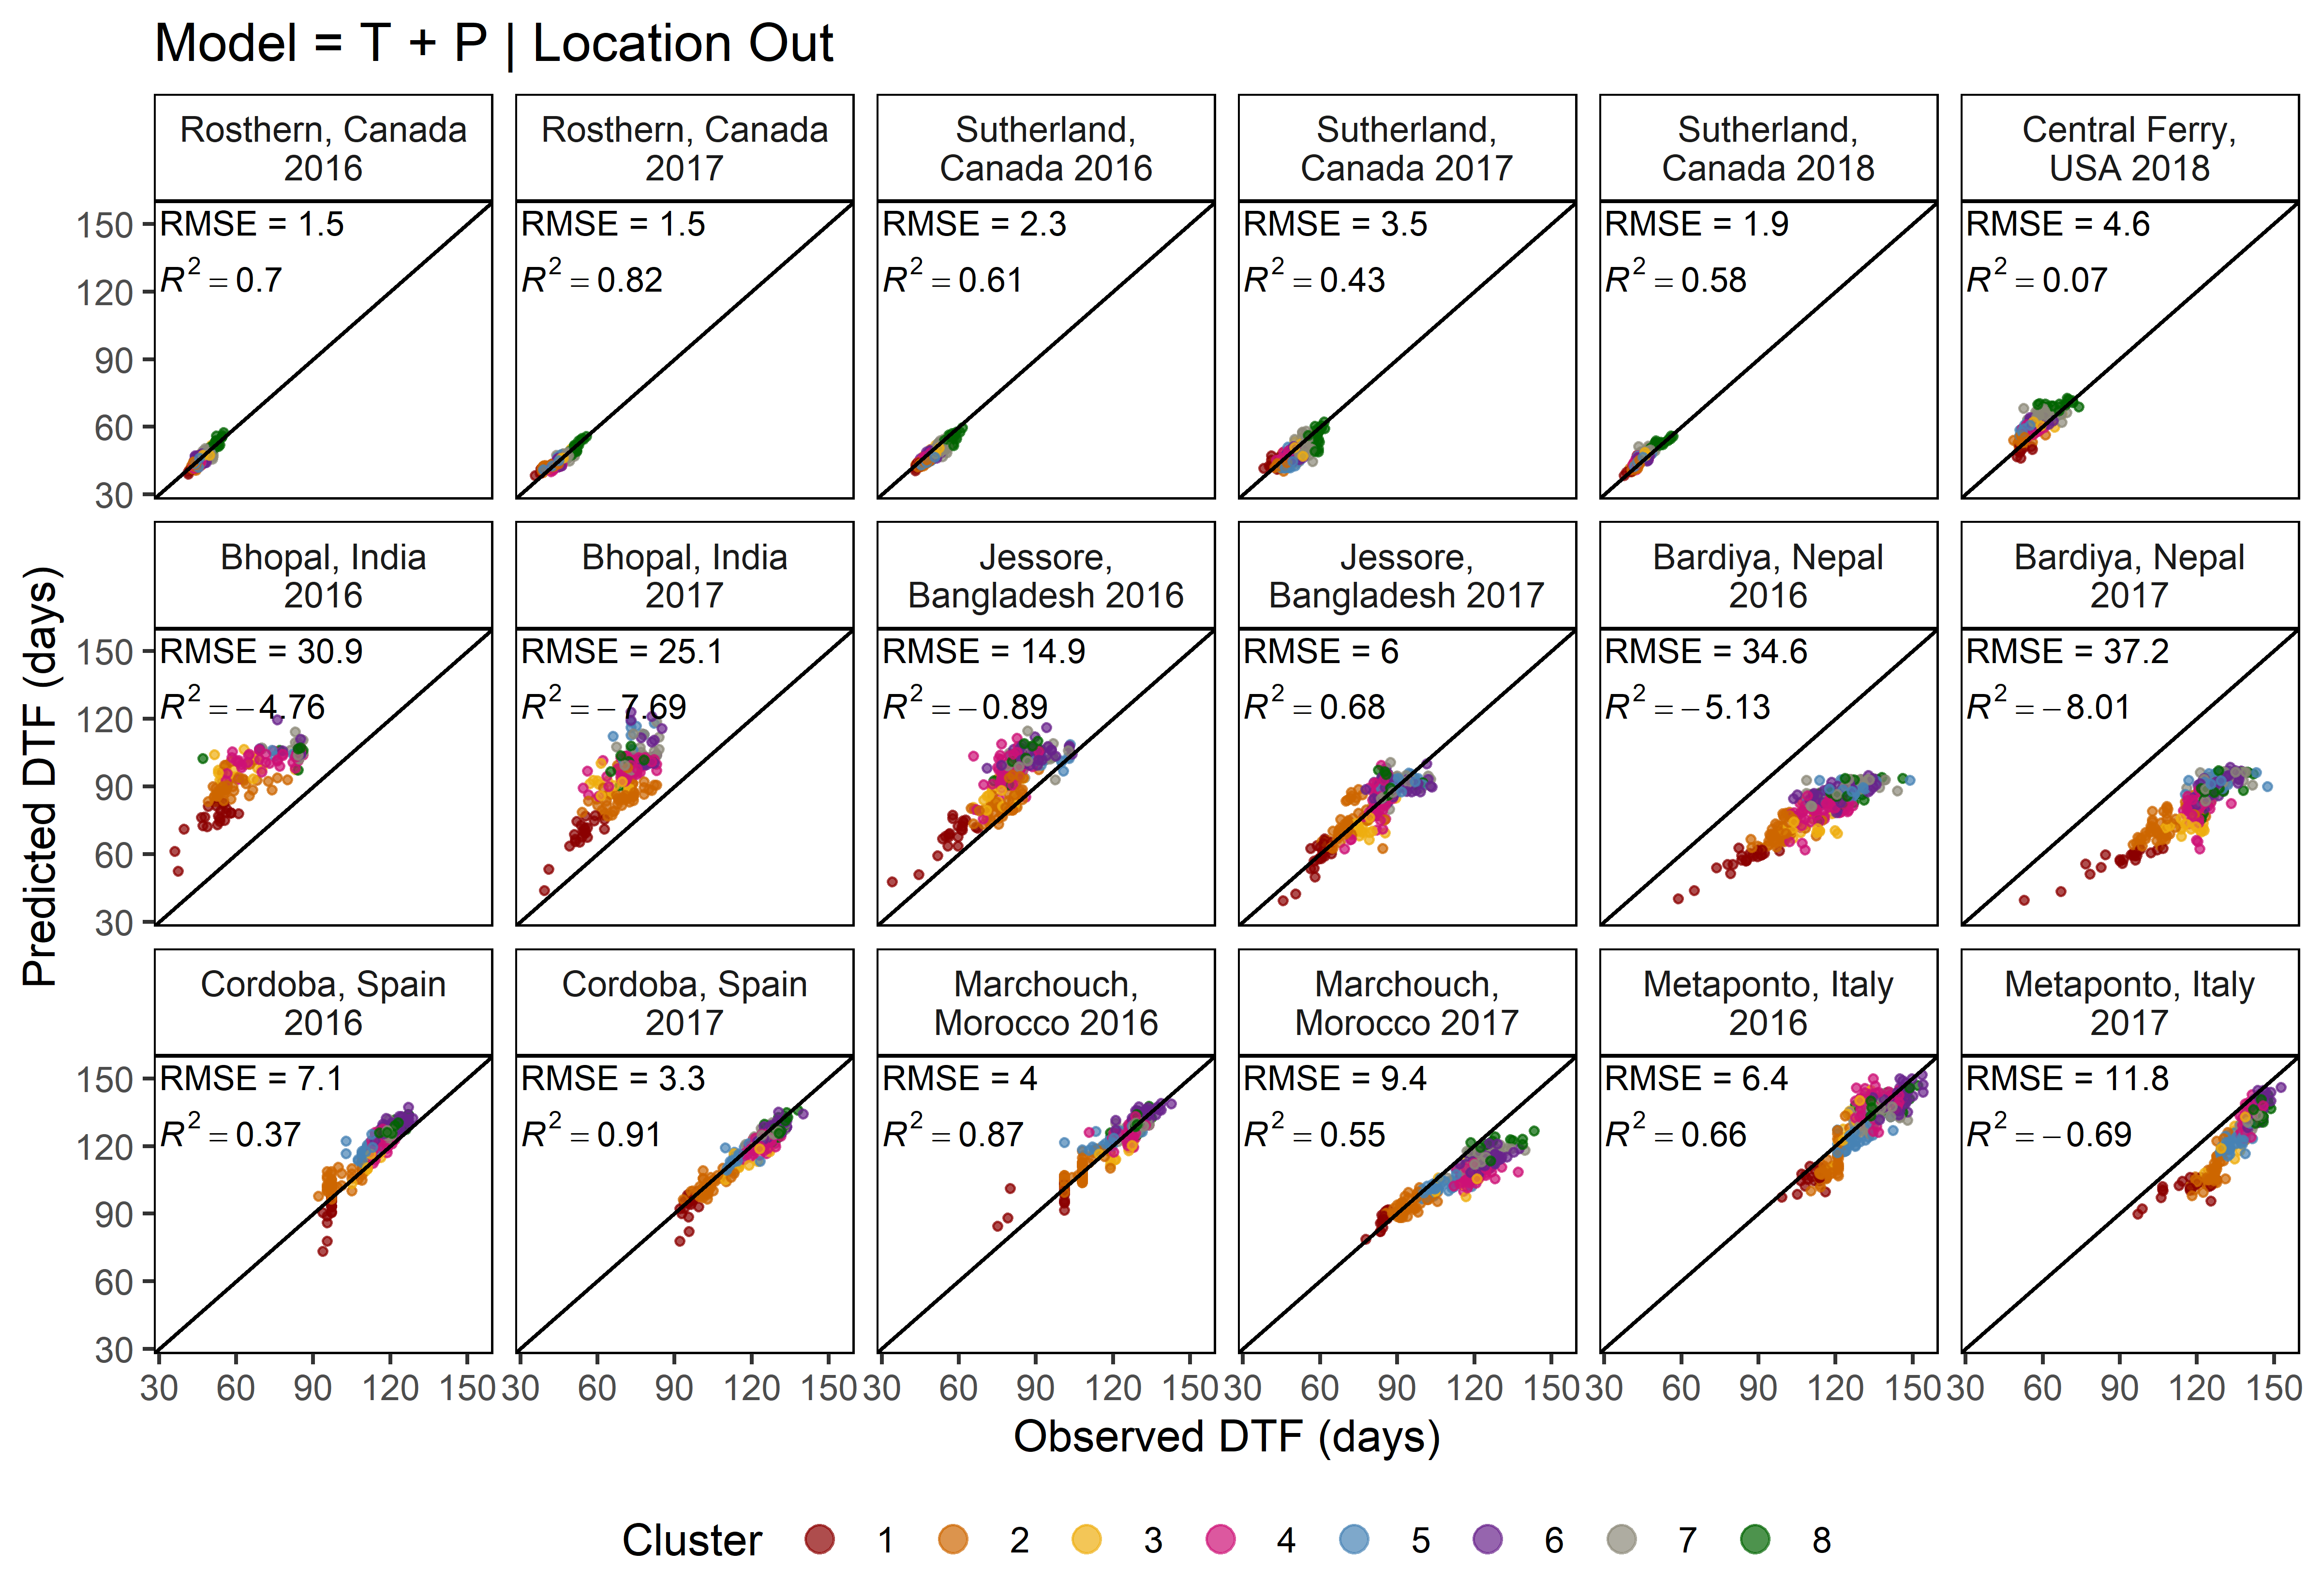
\includegraphics{Additional/Model/Model_2_3.png}

\hypertarget{supplemental-table-4-test-model}{%
\subsection{Supplemental Table 4 Test
Model}\label{supplemental-table-4-test-model}}

\begin{Shaded}
\begin{Highlighting}[]
\CommentTok{####################################}
\CommentTok{# 1/f = a + bT + cP (3 Locations) #}
\CommentTok{####################################}
\CommentTok{# Prep data}
\NormalTok{xx <-}\StringTok{ }\NormalTok{rr }\OperatorTok\StringTok{ }\CommentTok{#filter(!is.na(DTF)) %>%}
\StringTok{  }\KeywordTok{left_join}\NormalTok{(}\KeywordTok{select}\NormalTok{(ff, Expt, T_mean, P_mean), }\DataTypeTok{by =} \StringTok{"Expt"}\NormalTok{)}
\NormalTok{mt <-}\StringTok{ }\KeywordTok{data.frame}\NormalTok{(}\DataTypeTok{Temperate_Location     =} \KeywordTok{rep}\NormalTok{(names_ExptShort[}\DecValTok{1}\OperatorTok{:}\DecValTok{6}\NormalTok{],  }\DataTypeTok{each =} \DecValTok{36}\NormalTok{),}
                 \DataTypeTok{SouthAsian_Location    =} \KeywordTok{rep}\NormalTok{(names_ExptShort[}\DecValTok{7}\OperatorTok{:}\DecValTok{12}\NormalTok{], }\DataTypeTok{times =} \DecValTok{36}\NormalTok{)) }\OperatorTok
\StringTok{  }\KeywordTok{arrange}\NormalTok{(SouthAsian_Location) }\OperatorTok
\StringTok{  }\KeywordTok{mutate}\NormalTok{(}\DataTypeTok{Mediterranean_Location =} \KeywordTok{rep}\NormalTok{(names_ExptShort[}\DecValTok{13}\OperatorTok{:}\DecValTok{18}\NormalTok{], }\DecValTok{36}\NormalTok{),}
                 \DataTypeTok{RR =} \OtherTok{NA}\NormalTok{, }\DataTypeTok{Genotypes =} \OtherTok{NA}\NormalTok{)}
\CommentTok{# Run each combination}
\ControlFlowTok{for}\NormalTok{(t }\ControlFlowTok{in}\NormalTok{ names_ExptShort[}\DecValTok{1}\OperatorTok{:}\DecValTok{6}\NormalTok{]) \{ }\CommentTok{# Temperate site-years}
  \ControlFlowTok{for}\NormalTok{(s }\ControlFlowTok{in}\NormalTok{ names_ExptShort[}\DecValTok{7}\OperatorTok{:}\DecValTok{12}\NormalTok{]) \{ }\CommentTok{# South asian site-years}
    \ControlFlowTok{for}\NormalTok{(m }\ControlFlowTok{in}\NormalTok{ names_ExptShort[}\DecValTok{13}\OperatorTok{:}\DecValTok{18}\NormalTok{]) \{ }\CommentTok{# Mediterranean site-years}
\NormalTok{      mr <-}\StringTok{ }\OtherTok{NULL}\NormalTok{; md <-}\StringTok{ }\OtherTok{NULL}
      \ControlFlowTok{for}\NormalTok{(i }\ControlFlowTok{in} \DecValTok{1}\OperatorTok{:}\DecValTok{324}\NormalTok{) \{}
        \CommentTok{# Prep data}
\NormalTok{        xi1 <-}\StringTok{ }\NormalTok{xx }\OperatorTok\StringTok{ }\KeywordTok{filter}\NormalTok{(Entry }\OperatorTok{==}\StringTok{ }\NormalTok{i, ExptShort }\OperatorTok\StringTok{ }\KeywordTok{c}\NormalTok{(t, s, m))}
\NormalTok{        xi2 <-}\StringTok{ }\NormalTok{xx }\OperatorTok\StringTok{ }\KeywordTok{filter}\NormalTok{(Entry }\OperatorTok{==}\StringTok{ }\NormalTok{i)}
\NormalTok{        xd2 <-}\StringTok{ }\NormalTok{xi2 }\OperatorTok\StringTok{ }\KeywordTok{group_by}\NormalTok{(Entry, Name, Expt, ExptShort) }\OperatorTok\StringTok{ }
\StringTok{          }\KeywordTok{summarise_at}\NormalTok{(}\KeywordTok{vars}\NormalTok{(DTF, RDTF, T_mean, P_mean), }\KeywordTok{funs}\NormalTok{(mean), }\DataTypeTok{na.rm =}\NormalTok{ T) }\OperatorTok
\StringTok{          }\KeywordTok{ungroup}\NormalTok{()}
        \CommentTok{# Train model}
\NormalTok{        mi <-}\StringTok{ }\KeywordTok{lm}\NormalTok{(RDTF }\OperatorTok{~}\StringTok{ }\NormalTok{T_mean }\OperatorTok{+}\StringTok{ }\NormalTok{P_mean, }\DataTypeTok{data =}\NormalTok{ xi1)}
        \CommentTok{# Predict DTF}
\NormalTok{        xi2 <-}\StringTok{ }\NormalTok{xi2 }\OperatorTok\StringTok{ }\KeywordTok{mutate}\NormalTok{(}\DataTypeTok{Predicted_DTF =} \DecValTok{1} \OperatorTok{/}\StringTok{ }\KeywordTok{predict}\NormalTok{(mi, }\DataTypeTok{newdata =}\NormalTok{ xi2))}
\NormalTok{        xd2 <-}\StringTok{ }\NormalTok{xd2 }\OperatorTok\StringTok{ }\KeywordTok{mutate}\NormalTok{(}\DataTypeTok{Predicted_DTF =} \DecValTok{1} \OperatorTok{/}\StringTok{ }\KeywordTok{predict}\NormalTok{(mi, }\DataTypeTok{newdata =}\NormalTok{ xd2))}
        \CommentTok{# Save to table}
\NormalTok{        mr <-}\StringTok{ }\KeywordTok{bind_rows}\NormalTok{(mr, xi2)}
\NormalTok{        md <-}\StringTok{ }\KeywordTok{bind_rows}\NormalTok{(md, xd2)}
\NormalTok{      \}}
\NormalTok{      remEntries <-}\StringTok{ }\KeywordTok{unique}\NormalTok{(md}\OperatorTok{$}\NormalTok{Entry[}\KeywordTok{is.na}\NormalTok{(md}\OperatorTok{$}\NormalTok{DTF) }\OperatorTok{&}\StringTok{ }\NormalTok{md}\OperatorTok{$}\NormalTok{ExptShort }\OperatorTok\StringTok{ }\KeywordTok{c}\NormalTok{(t, s, m)])}
\NormalTok{      md2 <-}\StringTok{ }\NormalTok{md }\OperatorTok\StringTok{ }\KeywordTok{filter}\NormalTok{(}\OperatorTok{!}\NormalTok{Entry }\OperatorTok\StringTok{ }\NormalTok{remEntries, }\OperatorTok{!}\NormalTok{md}\OperatorTok{$}\NormalTok{ExptShort }\OperatorTok\StringTok{ }\KeywordTok{c}\NormalTok{(t, s, m))}
\NormalTok{      myrow <-}\StringTok{ }\NormalTok{mt}\OperatorTok{$}\NormalTok{Temperate_Location     }\OperatorTok{==}\StringTok{ }\NormalTok{t }\OperatorTok{&}\StringTok{ }
\StringTok{               }\NormalTok{mt}\OperatorTok{$}\NormalTok{SouthAsian_Location    }\OperatorTok{==}\StringTok{ }\NormalTok{s }\OperatorTok{&}\StringTok{ }
\StringTok{               }\NormalTok{mt}\OperatorTok{$}\NormalTok{Mediterranean_Location }\OperatorTok{==}\StringTok{ }\NormalTok{m}
\NormalTok{      mt[myrow,}\StringTok{"RR"}\NormalTok{] <-}\StringTok{ }\KeywordTok{round}\NormalTok{(}\KeywordTok{modelR2}\NormalTok{(md2}\OperatorTok{$}\NormalTok{DTF, md2}\OperatorTok{$}\NormalTok{Predicted_DTF), }\DecValTok{6}\NormalTok{)}
\NormalTok{      mt[myrow,}\StringTok{"Genotypes"}\NormalTok{] <-}\StringTok{ }\KeywordTok{length}\NormalTok{(}\KeywordTok{unique}\NormalTok{(md2}\OperatorTok{$}\NormalTok{Entry))}
\NormalTok{    \}}
\NormalTok{  \}}
\NormalTok{\}}
\CommentTok{# Save}
\KeywordTok{write.csv}\NormalTok{(mt }\OperatorTok\StringTok{ }\KeywordTok{arrange}\NormalTok{(RR), }\StringTok{"Supplemental_Table_04.csv"}\NormalTok{, }\DataTypeTok{row.names =}\NormalTok{ F)}
\end{Highlighting}
\end{Shaded}

\begin{longtable}[]{@{}llllrr@{}}
\toprule
& Temperate\_Location & SouthAsian\_Location & Mediterranean\_Location &
RR & Genotypes\tabularnewline
\midrule
\endhead
1 & Ro17 & In16 & Sp16 & 0.461770 & 159\tabularnewline
2 & Su18 & In16 & Sp16 & 0.462242 & 159\tabularnewline
3 & Ro16 & In16 & Sp16 & 0.466809 & 159\tabularnewline
4 & Su17 & In16 & Sp16 & 0.469932 & 159\tabularnewline
5 & Su16 & In16 & Sp16 & 0.473691 & 159\tabularnewline
6 & Ro17 & In16 & It17 & 0.475920 & 159\tabularnewline
211 & Ro17 & Ba17 & Sp17 & 0.858843 & 291\tabularnewline
212 & Su16 & Ba17 & Mo16 & 0.858923 & 291\tabularnewline
213 & Ro16 & Ba17 & Sp17 & 0.859936 & 291\tabularnewline
214 & Us18 & Ba17 & Sp17 & 0.861168 & 289\tabularnewline
215 & Su17 & Ba17 & Sp17 & 0.862977 & 291\tabularnewline
216 & Su16 & Ba17 & Sp17 & 0.863054 & 291\tabularnewline
\bottomrule
\end{longtable}

\hypertarget{modeling-dtf-t-p---3-best}{%
\subsection{Modeling DTF (T + P) - 3
Best}\label{modeling-dtf-t-p---3-best}}

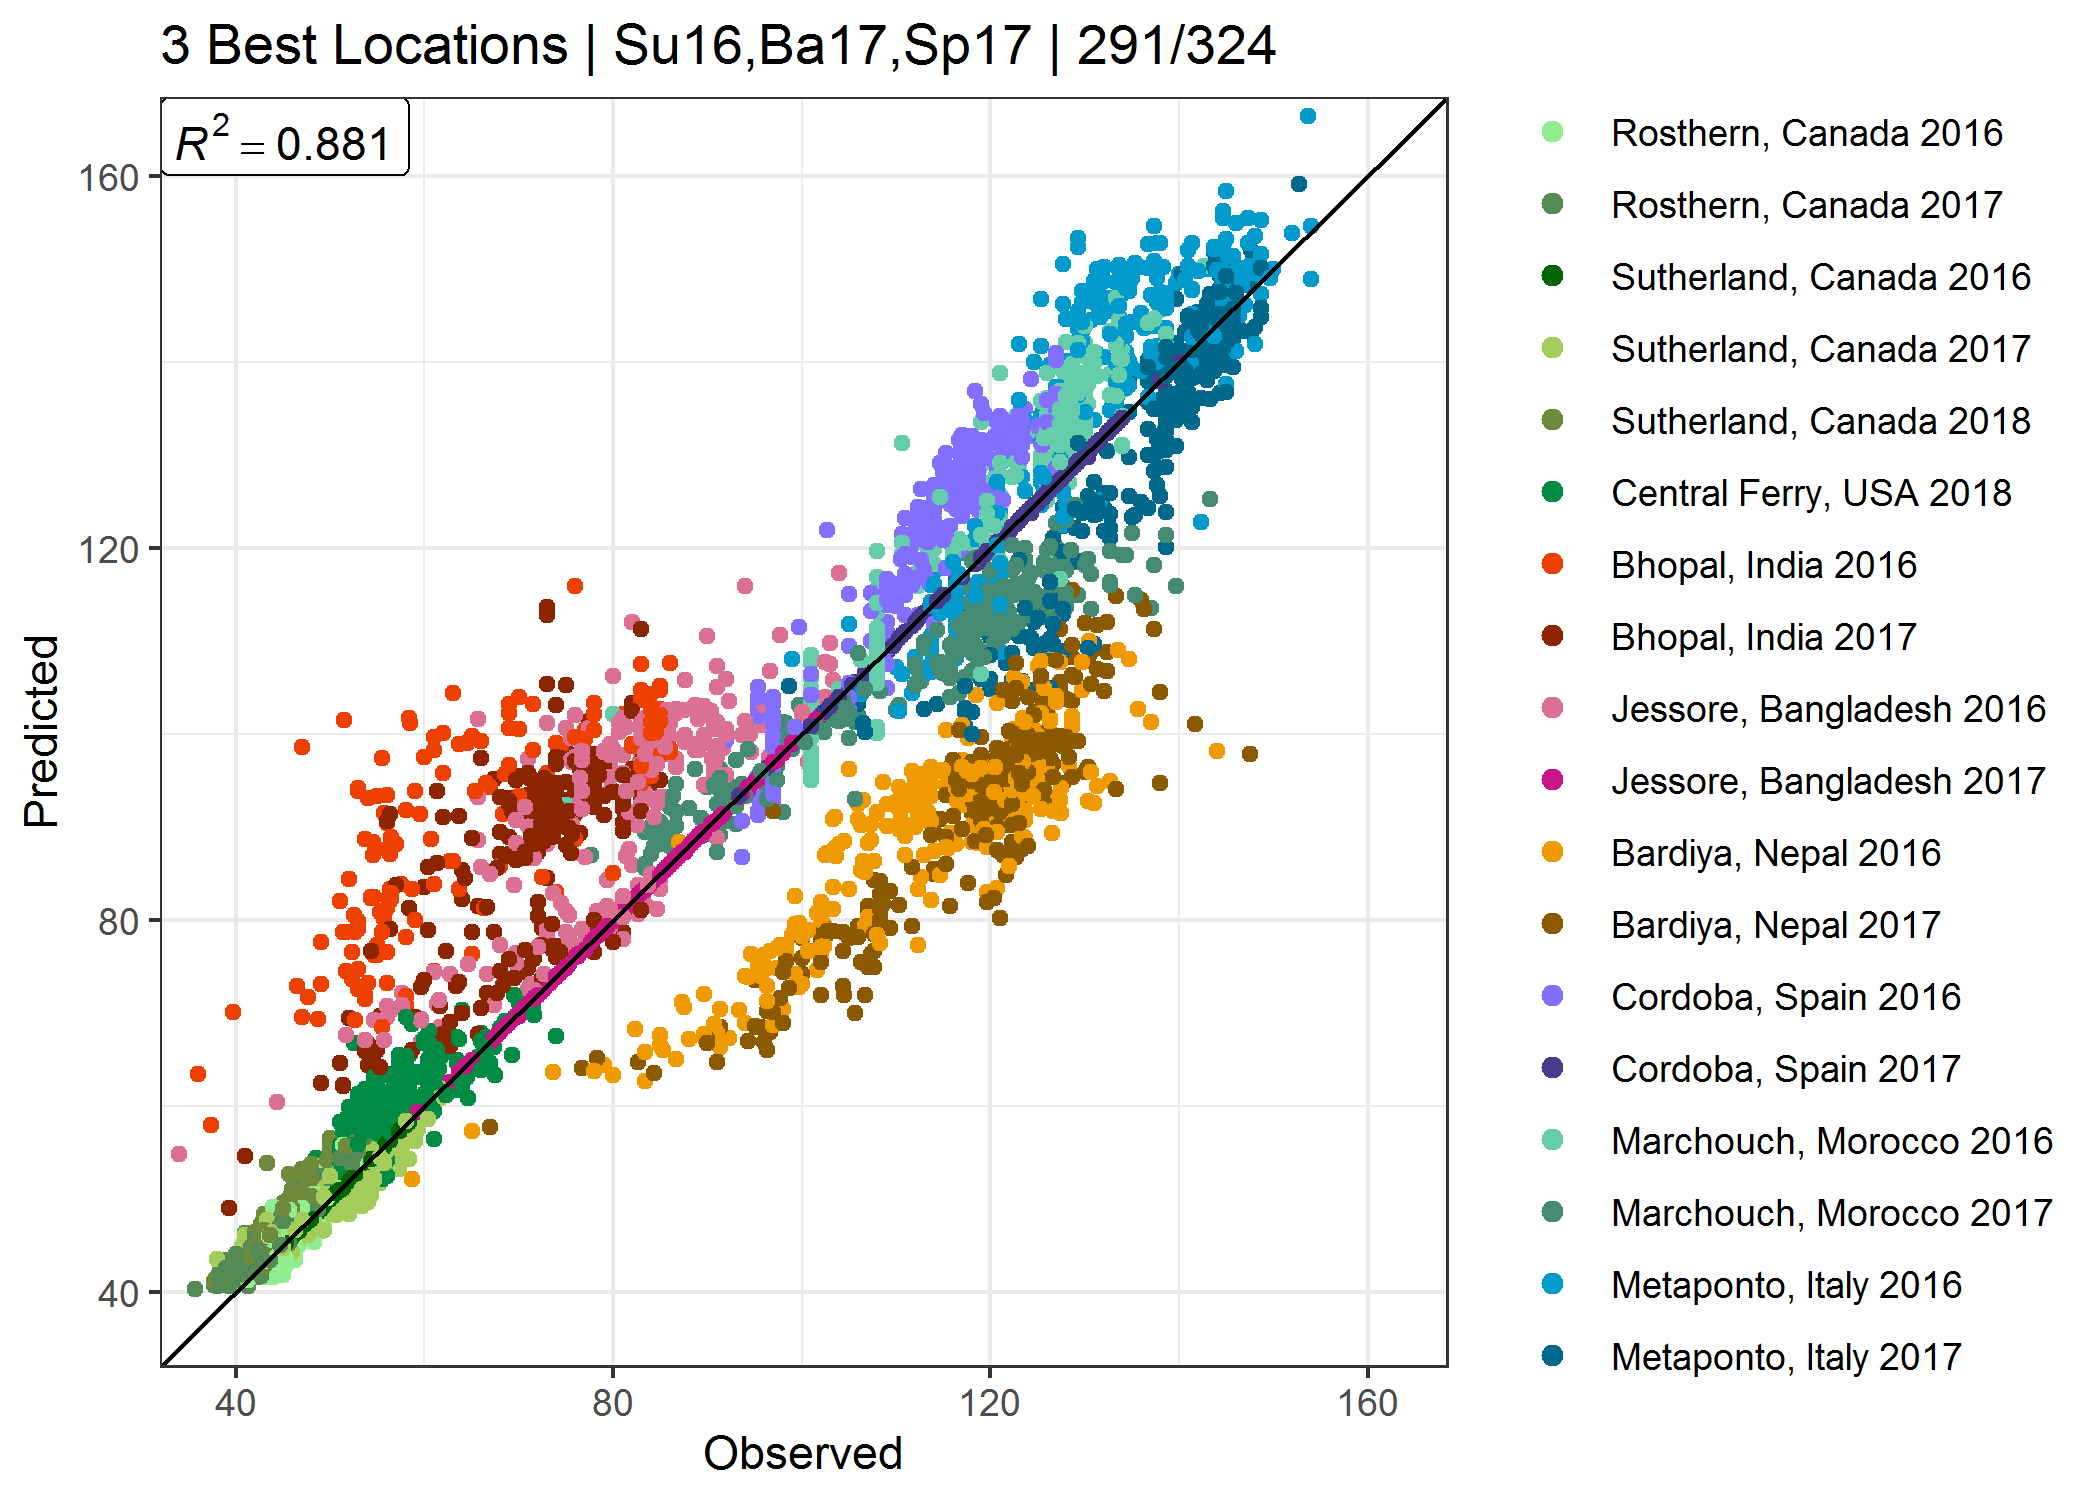
\includegraphics{Additional/Model/Model_1_4.png}

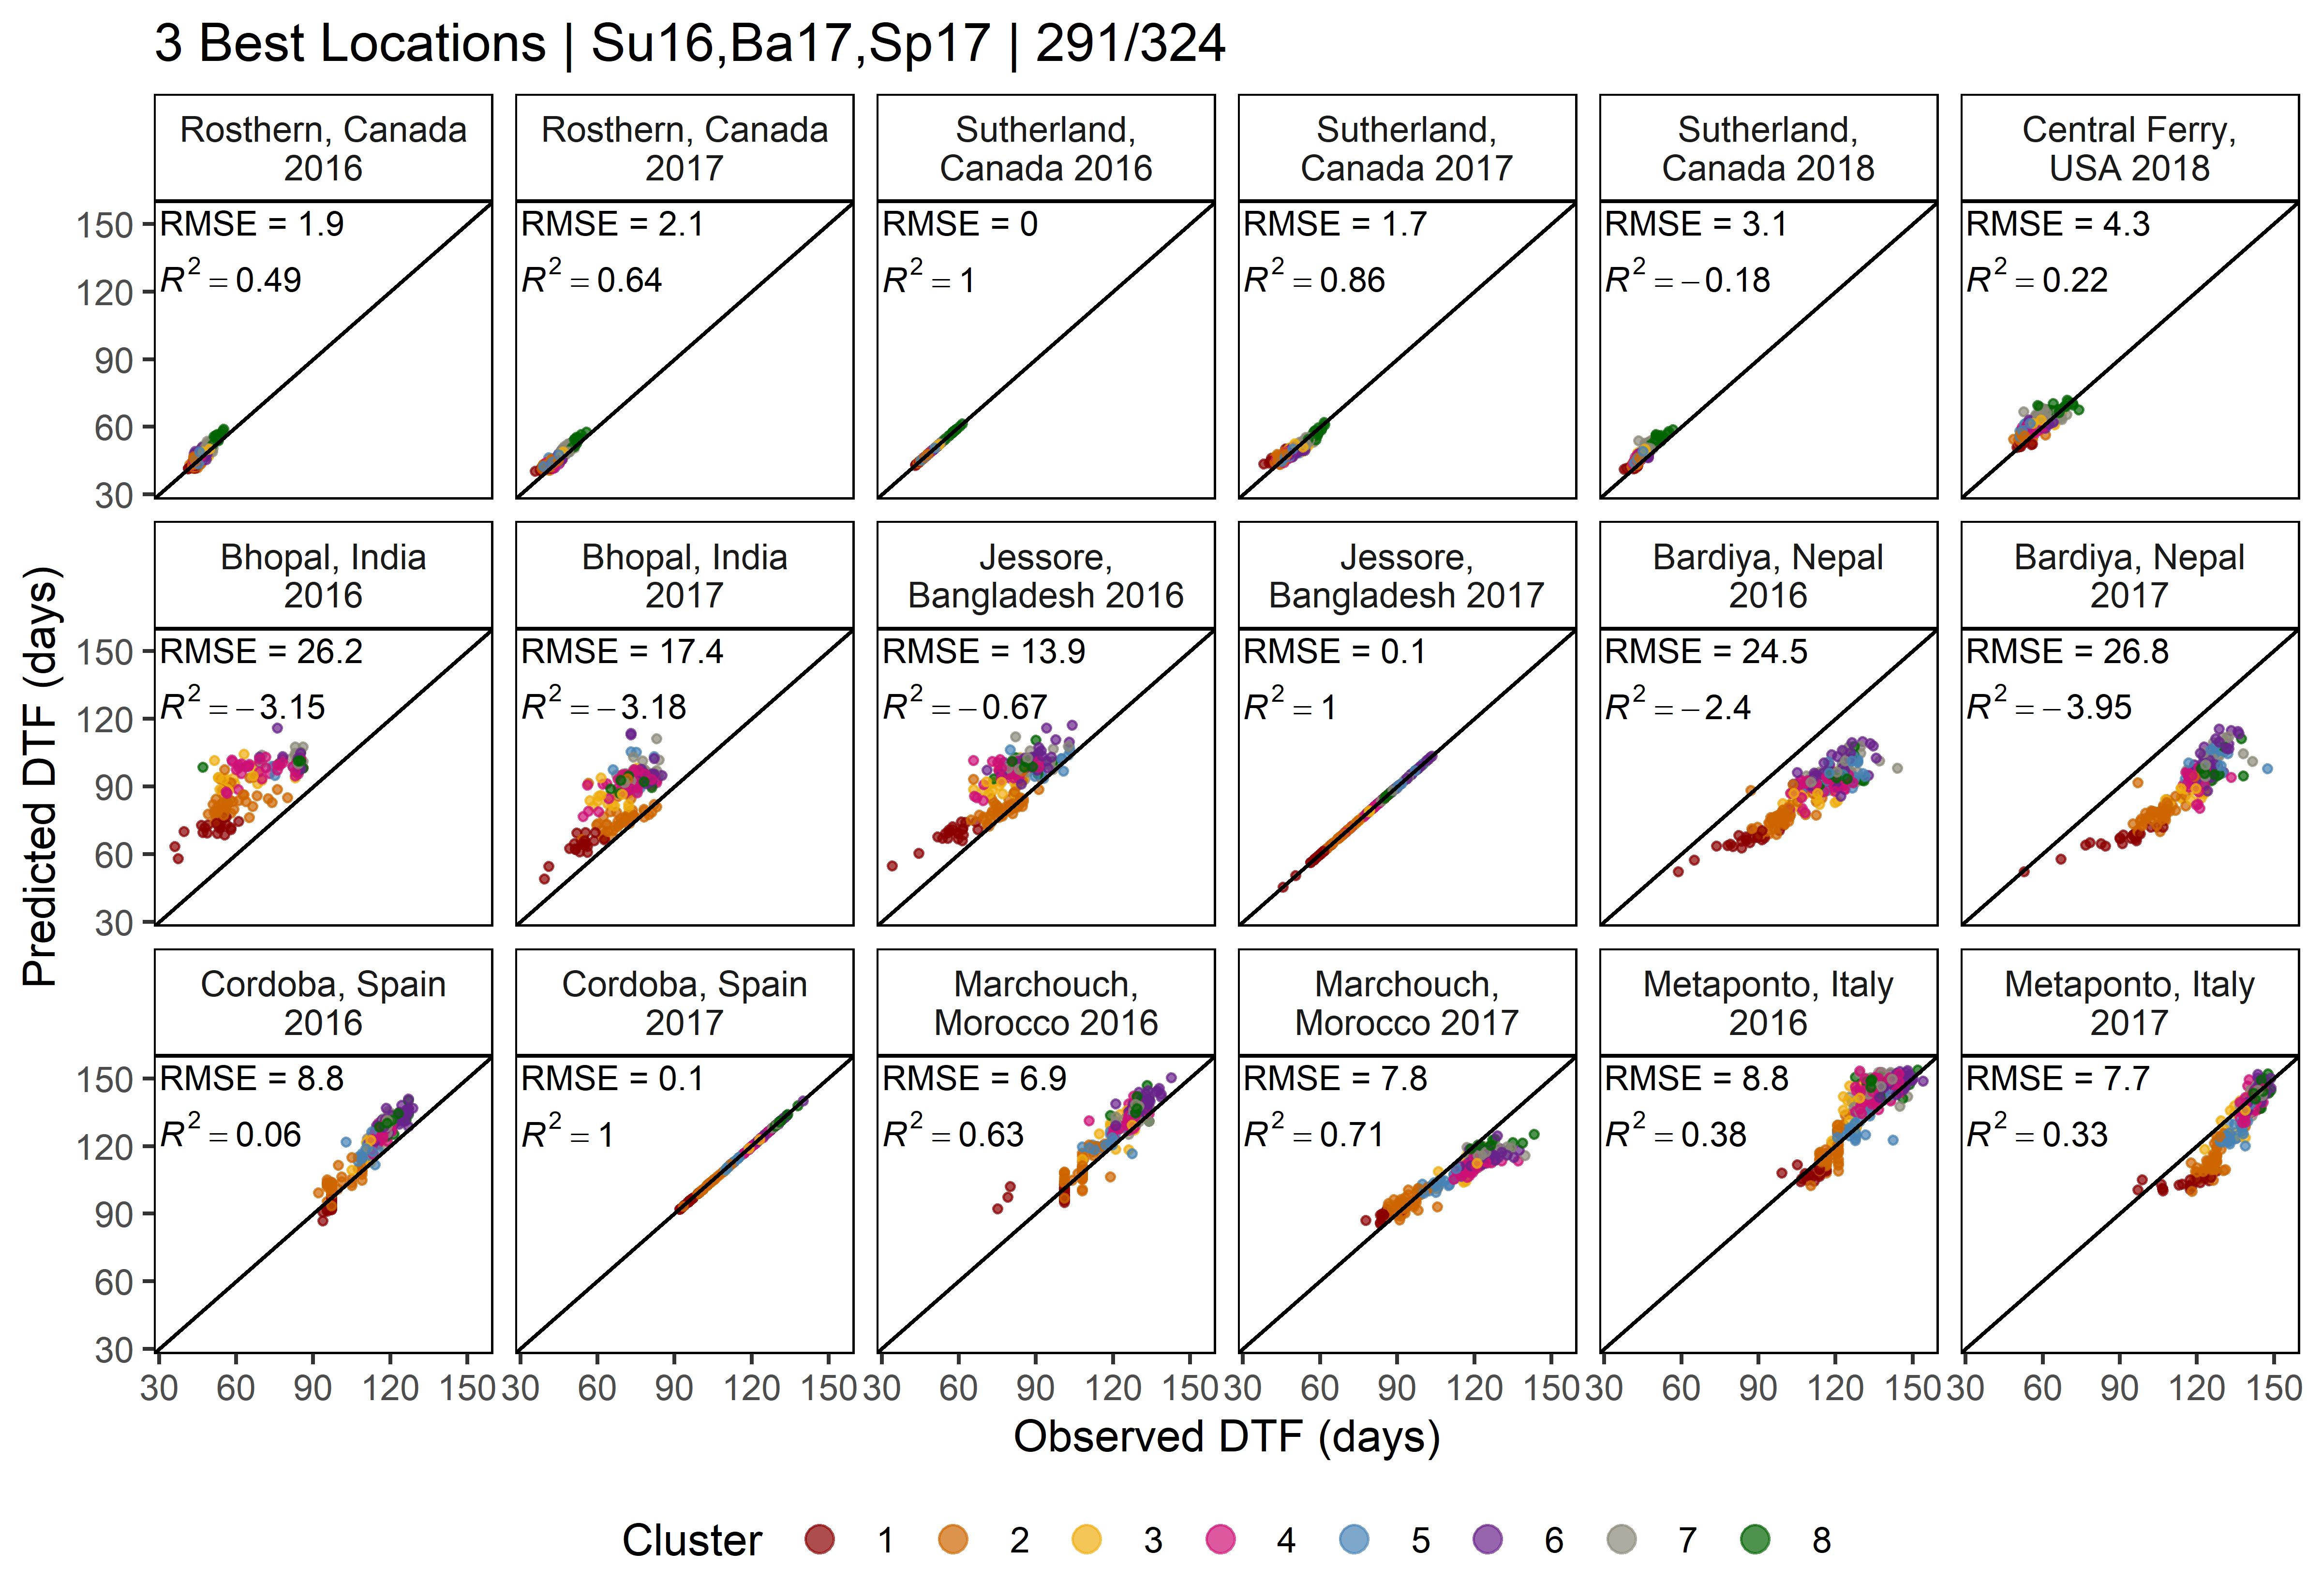
\includegraphics{Additional/Model/Model_2_4.png}

\begin{Shaded}
\begin{Highlighting}[]
\CommentTok{####################################}
\CommentTok{# 1/f = a + bT + cP (3 Locations) #}
\CommentTok{####################################}
\CommentTok{# Prep data}
\NormalTok{xx <-}\StringTok{ }\NormalTok{rr }\OperatorTok\StringTok{ }\KeywordTok{filter}\NormalTok{(}\OperatorTok{!}\KeywordTok{is.na}\NormalTok{(RDTF)) }\OperatorTok
\StringTok{  }\KeywordTok{left_join}\NormalTok{(}\KeywordTok{select}\NormalTok{(ff, Expt, T_mean, P_mean), }\DataTypeTok{by =} \StringTok{"Expt"}\NormalTok{)}
\NormalTok{mr <-}\StringTok{ }\OtherTok{NULL}\NormalTok{; md <-}\StringTok{ }\OtherTok{NULL}
\NormalTok{mc <-}\StringTok{ }\KeywordTok{select}\NormalTok{(ldp, Entry, Name) }\OperatorTok
\StringTok{  }\KeywordTok{mutate}\NormalTok{(}\DataTypeTok{a =} \OtherTok{NA}\NormalTok{, }\DataTypeTok{b =} \OtherTok{NA}\NormalTok{, }\DataTypeTok{c =} \OtherTok{NA}\NormalTok{, }\DataTypeTok{RR =} \OtherTok{NA}\NormalTok{, }\DataTypeTok{Environments =} \OtherTok{NA}\NormalTok{ )}
\NormalTok{k <-}\StringTok{ }\KeywordTok{c}\NormalTok{(}\StringTok{"Sutherland, Canada 2016"}\NormalTok{, }\StringTok{"Jessore, Bangladesh 2017"}\NormalTok{, }\StringTok{"Cordoba, Spain 2017"}\NormalTok{)}
\CommentTok{# Model - only the ^above^ three site-years are used to train the model}
\ControlFlowTok{for}\NormalTok{(i }\ControlFlowTok{in} \DecValTok{1}\OperatorTok{:}\DecValTok{324}\NormalTok{) \{}
  \CommentTok{# Prep data}
\NormalTok{  xi1 <-}\StringTok{ }\NormalTok{xx }\OperatorTok\StringTok{ }\KeywordTok{filter}\NormalTok{(Entry }\OperatorTok{==}\StringTok{ }\NormalTok{i, Expt }\OperatorTok\StringTok{ }\NormalTok{k)}
\NormalTok{  xi2 <-}\StringTok{ }\NormalTok{xx }\OperatorTok\StringTok{ }\KeywordTok{filter}\NormalTok{(Entry }\OperatorTok{==}\StringTok{ }\NormalTok{i)}
\NormalTok{  xd2 <-}\StringTok{ }\NormalTok{xi2 }\OperatorTok\StringTok{ }\KeywordTok{group_by}\NormalTok{(Entry, Name, Expt, ExptShort) }\OperatorTok\StringTok{ }
\StringTok{    }\KeywordTok{summarise_at}\NormalTok{(}\KeywordTok{vars}\NormalTok{(DTF, RDTF, T_mean, P_mean), }\KeywordTok{funs}\NormalTok{(mean), }\DataTypeTok{na.rm =}\NormalTok{ T) }\OperatorTok
\StringTok{    }\KeywordTok{ungroup}\NormalTok{()}
  \CommentTok{# Train model}
\NormalTok{  mi <-}\StringTok{ }\KeywordTok{lm}\NormalTok{(RDTF }\OperatorTok{~}\StringTok{ }\NormalTok{T_mean }\OperatorTok{*}\StringTok{ }\NormalTok{P_mean, }\DataTypeTok{data =}\NormalTok{ xi1)}
  \CommentTok{# Predict DTF}
\NormalTok{  xi2 <-}\StringTok{ }\NormalTok{xi2 }\OperatorTok\StringTok{ }\KeywordTok{mutate}\NormalTok{(}\DataTypeTok{Predicted_DTF =} \DecValTok{1} \OperatorTok{/}\StringTok{ }\KeywordTok{predict}\NormalTok{(mi, }\DataTypeTok{newdata =}\NormalTok{ xi2))}
\NormalTok{  xd2 <-}\StringTok{ }\NormalTok{xd2 }\OperatorTok\StringTok{ }\KeywordTok{mutate}\NormalTok{(}\DataTypeTok{Predicted_DTF =} \DecValTok{1} \OperatorTok{/}\StringTok{ }\KeywordTok{predict}\NormalTok{(mi, }\DataTypeTok{newdata =}\NormalTok{ xd2))}
  \CommentTok{# Save to table}
\NormalTok{  mr <-}\StringTok{ }\KeywordTok{bind_rows}\NormalTok{(mr, xi2)}
\NormalTok{  md <-}\StringTok{ }\KeywordTok{bind_rows}\NormalTok{(md, xd2)}
  \CommentTok{# Save coefficients}
\NormalTok{  mc[i,}\KeywordTok{c}\NormalTok{(}\DecValTok{3}\OperatorTok{:}\DecValTok{5}\NormalTok{)] <-}\StringTok{ }\NormalTok{mi}\OperatorTok{$}\NormalTok{coefficients}
  \CommentTok{# Calculate rr and # of environments used}
\NormalTok{  mc[i,}\DecValTok{6}\NormalTok{] <-}\StringTok{ }\DecValTok{1} \OperatorTok{-}\StringTok{ }\KeywordTok{sum}\NormalTok{((xi2}\OperatorTok{$}\NormalTok{DTF }\OperatorTok{-}\StringTok{ }\NormalTok{xi2}\OperatorTok{$}\NormalTok{Predicted_DTF)}\OperatorTok{^}\DecValTok{2}\NormalTok{) }\OperatorTok{/}\StringTok{ }
\StringTok{    }\KeywordTok{sum}\NormalTok{((xi2}\OperatorTok{$}\NormalTok{Predicted_DTF }\OperatorTok{-}\StringTok{ }\KeywordTok{mean}\NormalTok{(xi2}\OperatorTok{$}\NormalTok{DTF))}\OperatorTok{^}\DecValTok{2}\NormalTok{)}
\NormalTok{  mc[i,}\DecValTok{7}\NormalTok{] <-}\StringTok{ }\KeywordTok{length}\NormalTok{(}\KeywordTok{unique}\NormalTok{(xi2}\OperatorTok{$}\NormalTok{Expt))}
\NormalTok{\}}
\NormalTok{ents <-}\StringTok{ }\NormalTok{xx }\OperatorTok\StringTok{ }\KeywordTok{filter}\NormalTok{(ExptShort }\OperatorTok\StringTok{ }\KeywordTok{c}\NormalTok{(}\StringTok{"Su16"}\NormalTok{, }\StringTok{"Ba17"}\NormalTok{, }\StringTok{"Sp17"}\NormalTok{), }\KeywordTok{is.na}\NormalTok{(DTF)) }\OperatorTok
\StringTok{  }\KeywordTok{pull}\NormalTok{(Entry) }\OperatorTok\StringTok{ }\KeywordTok{unique}\NormalTok{()}
\NormalTok{mr <-}\StringTok{ }\NormalTok{mr }\OperatorTok\StringTok{ }\KeywordTok{filter}\NormalTok{(}\OperatorTok{!}\NormalTok{Entry }\OperatorTok\StringTok{ }\NormalTok{ents)}
\NormalTok{md <-}\StringTok{ }\NormalTok{md }\OperatorTok\StringTok{ }\KeywordTok{filter}\NormalTok{(}\OperatorTok{!}\NormalTok{Entry }\OperatorTok\StringTok{ }\NormalTok{ents)}
\NormalTok{mc <-}\StringTok{ }\NormalTok{mc }\OperatorTok\StringTok{ }\KeywordTok{filter}\NormalTok{(}\OperatorTok{!}\NormalTok{Entry }\OperatorTok\StringTok{ }\NormalTok{ents)}
\CommentTok{# Save Results}
\KeywordTok{write.csv}\NormalTok{(mr, }\StringTok{"data/model_3best.csv"}\NormalTok{,        }\DataTypeTok{row.names =}\NormalTok{ F)}
\KeywordTok{write.csv}\NormalTok{(md, }\StringTok{"data/model_3best_d.csv"}\NormalTok{,      }\DataTypeTok{row.names =}\NormalTok{ F)}
\KeywordTok{write.csv}\NormalTok{(mc, }\StringTok{"data/model_3best_coefs.csv"}\NormalTok{,  }\DataTypeTok{row.names =}\NormalTok{ F)}
\end{Highlighting}
\end{Shaded}

\begin{Shaded}
\begin{Highlighting}[]
\CommentTok{# Prep data }
\NormalTok{xx <-}\StringTok{ }\KeywordTok{read.csv}\NormalTok{(}\StringTok{"data/model_3best_d.csv"}\NormalTok{) }\OperatorTok\StringTok{ }
\StringTok{  }\KeywordTok{mutate}\NormalTok{(}\DataTypeTok{Expt =} \KeywordTok{factor}\NormalTok{(Expt, }\DataTypeTok{levels =}\NormalTok{ names_Expt))}
\KeywordTok{length}\NormalTok{(}\KeywordTok{unique}\NormalTok{(xx}\OperatorTok{$}\NormalTok{Entry))}
\end{Highlighting}
\end{Shaded}

\begin{verbatim}
[1] 291
\end{verbatim}

\begin{Shaded}
\begin{Highlighting}[]
\CommentTok{# Plot Observed vs Predicted}
\NormalTok{mp <-}\StringTok{ }\KeywordTok{gg_model_1}\NormalTok{(xx, }\DataTypeTok{title =} \StringTok{"3 Best Locations | Su16,Ba17,Sp17 | 291/324"}\NormalTok{)}
\KeywordTok{ggsave}\NormalTok{(}\StringTok{"Additional/Model/Model_1_4.png"}\NormalTok{, mp, }\DataTypeTok{width =} \DecValTok{7}\NormalTok{, }\DataTypeTok{height =} \DecValTok{5}\NormalTok{, }\DataTypeTok{dpi =} \DecValTok{600}\NormalTok{)}
\end{Highlighting}
\end{Shaded}

\begin{Shaded}
\begin{Highlighting}[]
\CommentTok{# Plot B)}
\NormalTok{mp <-}\StringTok{ }\KeywordTok{gg_model_2}\NormalTok{(xx, }\DataTypeTok{title =} \StringTok{"3 Best Locations | Su16,Ba17,Sp17 | 291/324"}\NormalTok{)}
\KeywordTok{ggsave}\NormalTok{(}\StringTok{"Additional/Model/Model_2_4.png"}\NormalTok{, mp, }\DataTypeTok{width =} \DecValTok{8}\NormalTok{, }\DataTypeTok{height =} \FloatTok{5.5}\NormalTok{, }\DataTypeTok{dpi =} \DecValTok{600}\NormalTok{)}
\end{Highlighting}
\end{Shaded}

\hypertarget{modeling-dtf-t-p---3-worst}{%
\subsection{Modeling DTF (T + P) - 3
Worst}\label{modeling-dtf-t-p---3-worst}}

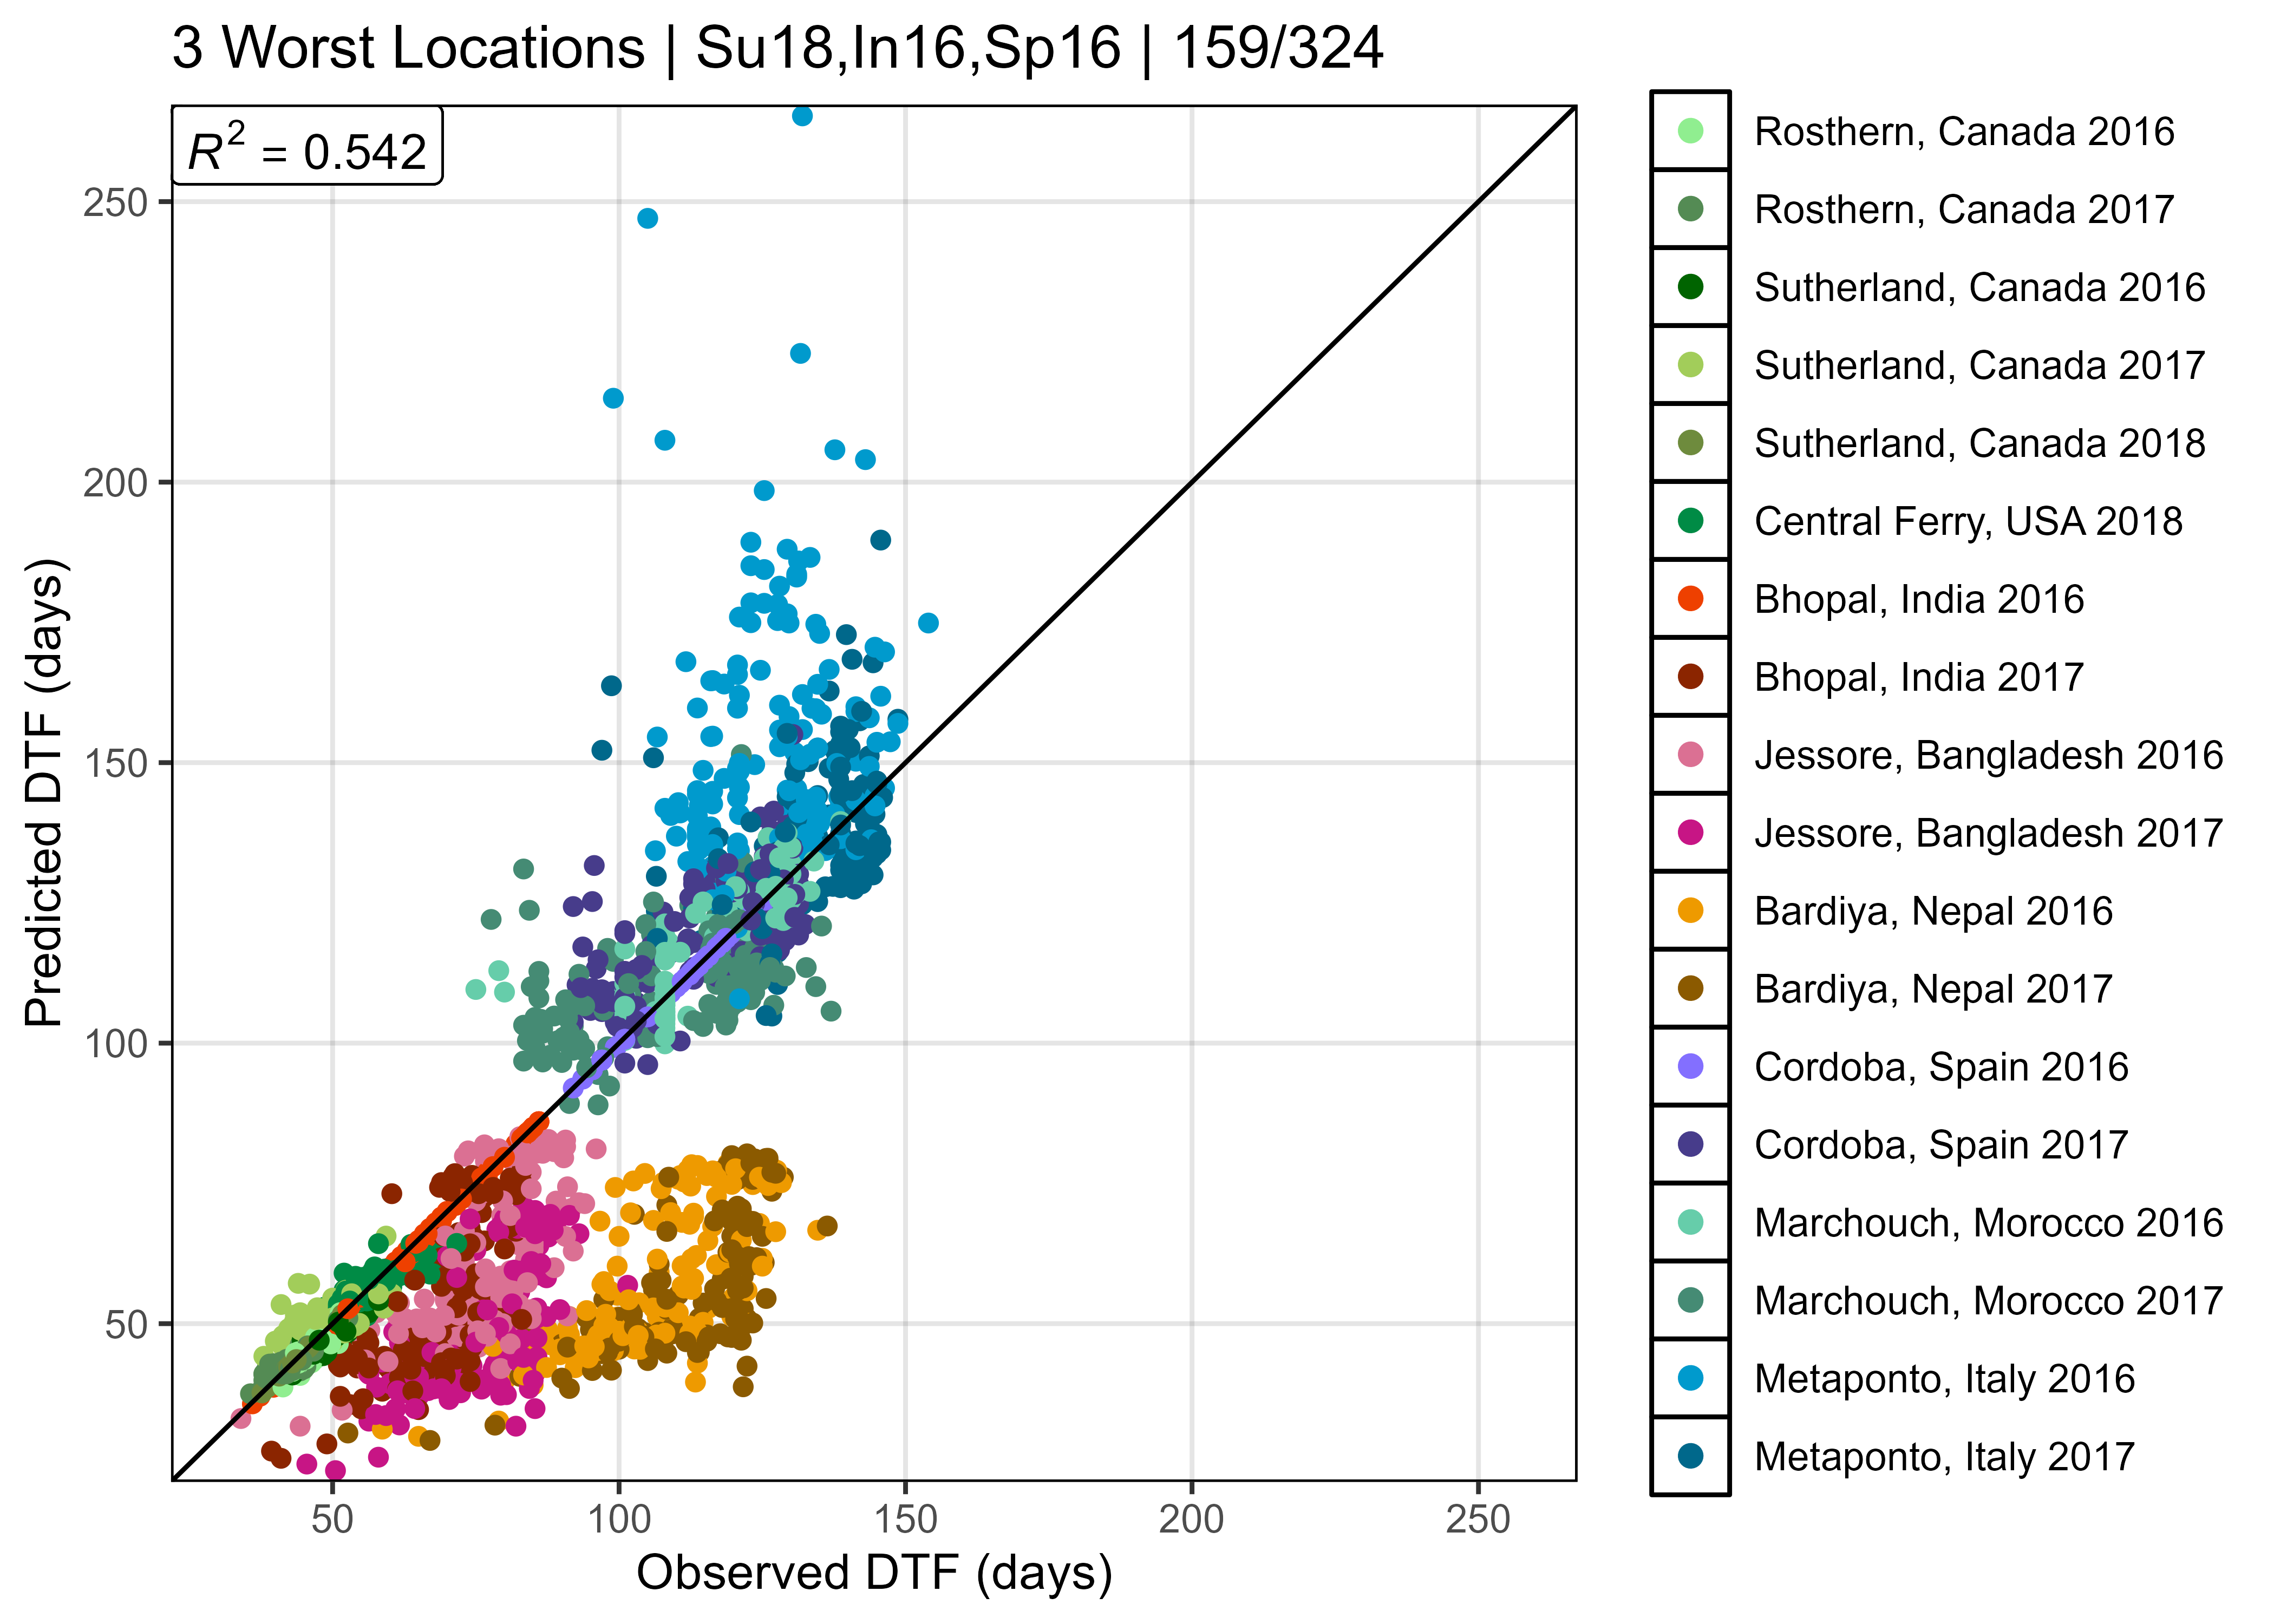
\includegraphics{Additional/Model/Model_1_5.png}

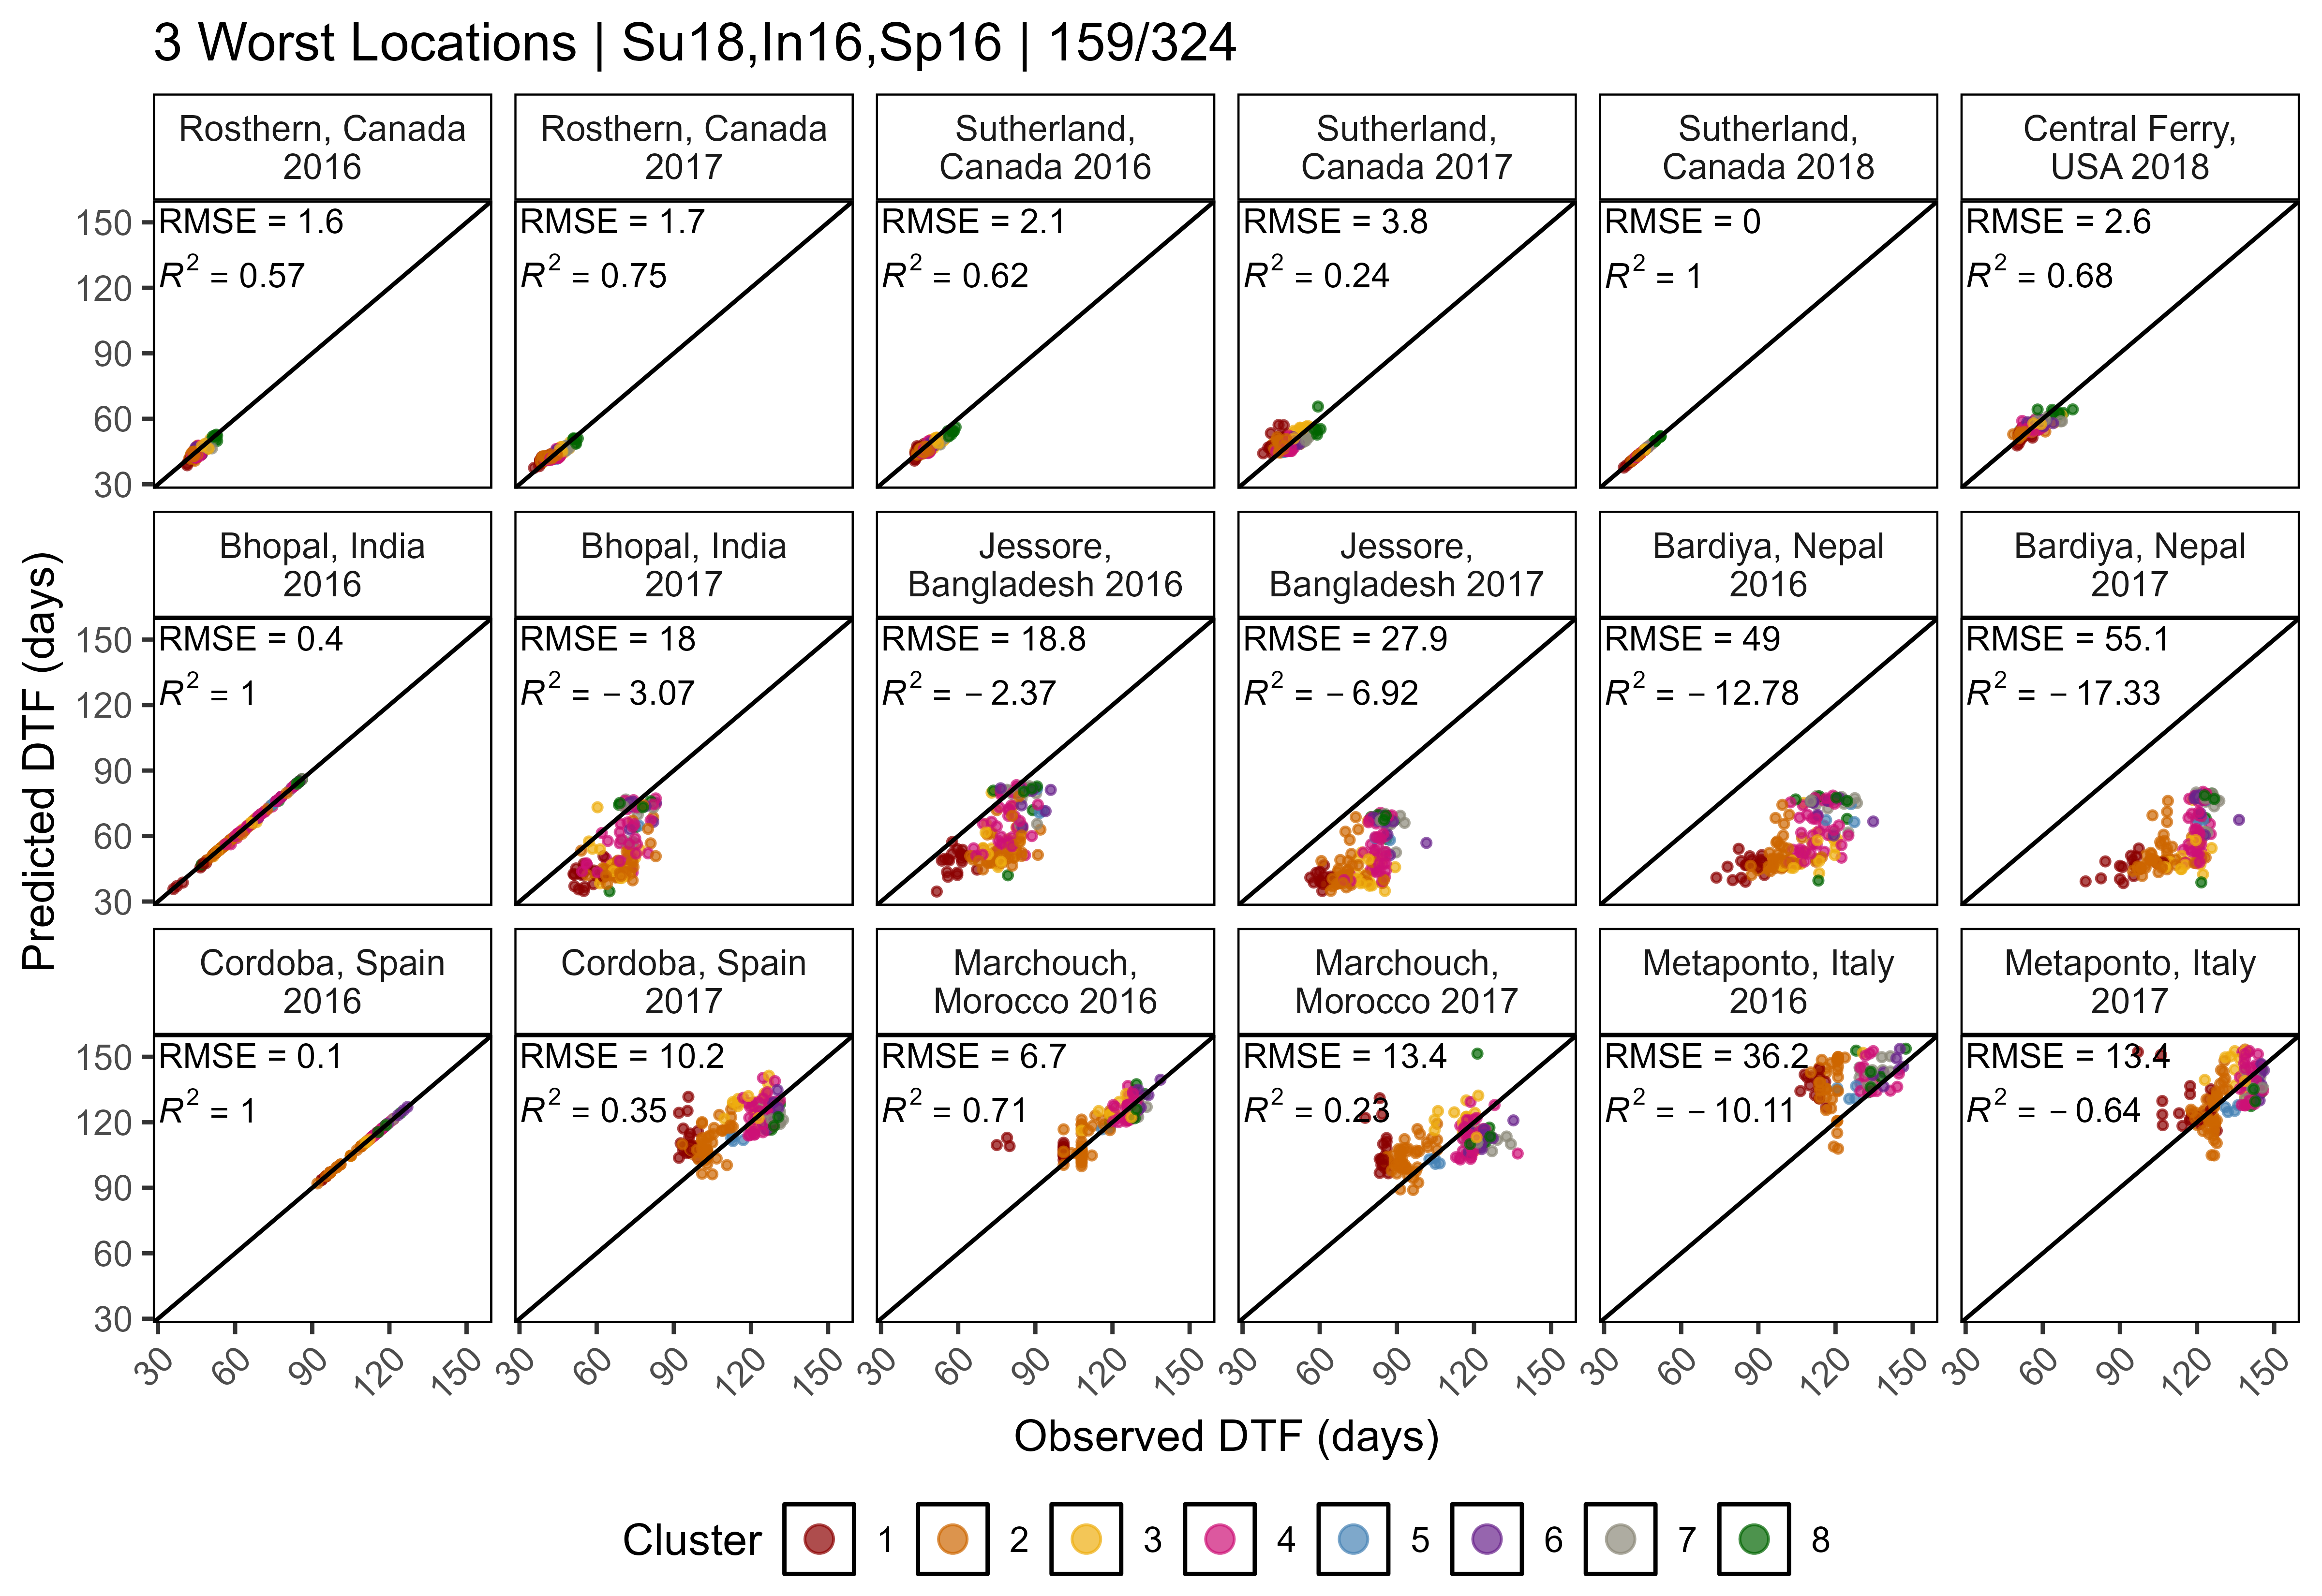
\includegraphics{Additional/Model/Model_2_5.png}

\begin{Shaded}
\begin{Highlighting}[]
\CommentTok{####################################}
\CommentTok{# 1/f = a + bT + cP (3 Locations)  #}
\CommentTok{####################################}
\CommentTok{# Prep data}
\NormalTok{xx <-}\StringTok{ }\NormalTok{rr }\OperatorTok\StringTok{ }\KeywordTok{filter}\NormalTok{(}\OperatorTok{!}\KeywordTok{is.na}\NormalTok{(RDTF)) }\OperatorTok
\StringTok{  }\KeywordTok{left_join}\NormalTok{(}\KeywordTok{select}\NormalTok{(ff, Expt, T_mean, P_mean), }\DataTypeTok{by =} \StringTok{"Expt"}\NormalTok{)}
\NormalTok{mr <-}\StringTok{ }\OtherTok{NULL}\NormalTok{; md <-}\StringTok{ }\OtherTok{NULL}
\NormalTok{mc <-}\StringTok{ }\KeywordTok{select}\NormalTok{(ldp, Entry, Name) }\OperatorTok
\StringTok{  }\KeywordTok{mutate}\NormalTok{(}\DataTypeTok{a =} \OtherTok{NA}\NormalTok{, }\DataTypeTok{b =} \OtherTok{NA}\NormalTok{, }\DataTypeTok{c =} \OtherTok{NA}\NormalTok{, }\DataTypeTok{RR =} \OtherTok{NA}\NormalTok{, }\DataTypeTok{Environments =} \OtherTok{NA}\NormalTok{ )}
\NormalTok{k <-}\StringTok{ }\KeywordTok{c}\NormalTok{(}\StringTok{"Sutherland, Canada 2018"}\NormalTok{, }\StringTok{"Bhopal, India 2016"}\NormalTok{, }\StringTok{"Cordoba, Spain 2016"}\NormalTok{)}
\CommentTok{# Model - only the ^above^ three site-years are used to train the model}
\ControlFlowTok{for}\NormalTok{(i }\ControlFlowTok{in} \DecValTok{1}\OperatorTok{:}\DecValTok{324}\NormalTok{) \{}
  \CommentTok{# Prep data}
\NormalTok{  xi1 <-}\StringTok{ }\NormalTok{xx }\OperatorTok\StringTok{ }\KeywordTok{filter}\NormalTok{(Entry }\OperatorTok{==}\StringTok{ }\NormalTok{i, Expt }\OperatorTok\StringTok{ }\NormalTok{k)}
\NormalTok{  xi2 <-}\StringTok{ }\NormalTok{xx }\OperatorTok\StringTok{ }\KeywordTok{filter}\NormalTok{(Entry }\OperatorTok{==}\StringTok{ }\NormalTok{i)}
\NormalTok{  xd2 <-}\StringTok{ }\NormalTok{xi2 }\OperatorTok\StringTok{ }\KeywordTok{group_by}\NormalTok{(Entry, Name, Expt, ExptShort) }\OperatorTok\StringTok{ }
\StringTok{    }\KeywordTok{summarise_at}\NormalTok{(}\KeywordTok{vars}\NormalTok{(DTF, RDTF, T_mean, P_mean), }\KeywordTok{funs}\NormalTok{(mean), }\DataTypeTok{na.rm =}\NormalTok{ T) }\OperatorTok
\StringTok{    }\KeywordTok{ungroup}\NormalTok{()}
  \CommentTok{# Train model}
\NormalTok{  mi <-}\StringTok{ }\KeywordTok{lm}\NormalTok{(RDTF }\OperatorTok{~}\StringTok{ }\NormalTok{T_mean }\OperatorTok{*}\StringTok{ }\NormalTok{P_mean, }\DataTypeTok{data =}\NormalTok{ xi1)}
  \CommentTok{# Predict DTF}
\NormalTok{  xi2 <-}\StringTok{ }\NormalTok{xi2 }\OperatorTok\StringTok{ }\KeywordTok{mutate}\NormalTok{(}\DataTypeTok{Predicted_DTF =} \DecValTok{1} \OperatorTok{/}\StringTok{ }\KeywordTok{predict}\NormalTok{(mi, }\DataTypeTok{newdata =}\NormalTok{ xi2))}
\NormalTok{  xd2 <-}\StringTok{ }\NormalTok{xd2 }\OperatorTok\StringTok{ }\KeywordTok{mutate}\NormalTok{(}\DataTypeTok{Predicted_DTF =} \DecValTok{1} \OperatorTok{/}\StringTok{ }\KeywordTok{predict}\NormalTok{(mi, }\DataTypeTok{newdata =}\NormalTok{ xd2))}
  \CommentTok{# Save to table}
\NormalTok{  mr <-}\StringTok{ }\KeywordTok{bind_rows}\NormalTok{(mr, xi2)}
\NormalTok{  md <-}\StringTok{ }\KeywordTok{bind_rows}\NormalTok{(md, xd2)}
  \CommentTok{# Save coefficients}
\NormalTok{  mc[i,}\KeywordTok{c}\NormalTok{(}\DecValTok{3}\OperatorTok{:}\DecValTok{5}\NormalTok{)] <-}\StringTok{ }\NormalTok{mi}\OperatorTok{$}\NormalTok{coefficients}
  \CommentTok{# Calculate rr and # of environments used}
\NormalTok{  mc[i,}\DecValTok{6}\NormalTok{] <-}\StringTok{ }\DecValTok{1} \OperatorTok{-}\StringTok{ }\KeywordTok{sum}\NormalTok{((xi2}\OperatorTok{$}\NormalTok{DTF }\OperatorTok{-}\StringTok{ }\NormalTok{xi2}\OperatorTok{$}\NormalTok{Predicted_DTF)}\OperatorTok{^}\DecValTok{2}\NormalTok{) }\OperatorTok{/}\StringTok{ }
\StringTok{    }\KeywordTok{sum}\NormalTok{((xi2}\OperatorTok{$}\NormalTok{Predicted_DTF }\OperatorTok{-}\StringTok{ }\KeywordTok{mean}\NormalTok{(xi2}\OperatorTok{$}\NormalTok{DTF))}\OperatorTok{^}\DecValTok{2}\NormalTok{)}
\NormalTok{  mc[i,}\DecValTok{7}\NormalTok{] <-}\StringTok{ }\KeywordTok{length}\NormalTok{(}\KeywordTok{unique}\NormalTok{(xi2}\OperatorTok{$}\NormalTok{Expt))}
\NormalTok{\}}
\NormalTok{ents <-}\StringTok{ }\NormalTok{xx }\OperatorTok\StringTok{ }\KeywordTok{filter}\NormalTok{(ExptShort }\OperatorTok\StringTok{ }\KeywordTok{c}\NormalTok{(}\StringTok{"Su18"}\NormalTok{, }\StringTok{"In16"}\NormalTok{, }\StringTok{"Sp16"}\NormalTok{), }\KeywordTok{is.na}\NormalTok{(DTF)) }\OperatorTok
\StringTok{  }\KeywordTok{pull}\NormalTok{(Entry) }\OperatorTok\StringTok{ }\KeywordTok{unique}\NormalTok{()}
\NormalTok{mr <-}\StringTok{ }\NormalTok{mr }\OperatorTok\StringTok{ }\KeywordTok{filter}\NormalTok{(}\OperatorTok{!}\NormalTok{Entry }\OperatorTok\StringTok{ }\NormalTok{ents)}
\NormalTok{md <-}\StringTok{ }\NormalTok{md }\OperatorTok\StringTok{ }\KeywordTok{filter}\NormalTok{(}\OperatorTok{!}\NormalTok{Entry }\OperatorTok\StringTok{ }\NormalTok{ents)}
\NormalTok{mc <-}\StringTok{ }\NormalTok{mc }\OperatorTok\StringTok{ }\KeywordTok{filter}\NormalTok{(}\OperatorTok{!}\NormalTok{Entry }\OperatorTok\StringTok{ }\NormalTok{ents)}
\CommentTok{# Save Results}
\KeywordTok{write.csv}\NormalTok{(mr, }\StringTok{"data/model_3worst.csv"}\NormalTok{,        }\DataTypeTok{row.names =}\NormalTok{ F)}
\KeywordTok{write.csv}\NormalTok{(md, }\StringTok{"data/model_3worst_d.csv"}\NormalTok{,      }\DataTypeTok{row.names =}\NormalTok{ F)}
\KeywordTok{write.csv}\NormalTok{(mc, }\StringTok{"data/model_3worst_coefs.csv"}\NormalTok{,  }\DataTypeTok{row.names =}\NormalTok{ F)}
\end{Highlighting}
\end{Shaded}

\begin{Shaded}
\begin{Highlighting}[]
\CommentTok{# Prep data }
\NormalTok{xx <-}\StringTok{ }\KeywordTok{read.csv}\NormalTok{(}\StringTok{"data/model_3worst_d.csv"}\NormalTok{) }\OperatorTok\StringTok{ }
\StringTok{  }\KeywordTok{mutate}\NormalTok{(}\DataTypeTok{Expt =} \KeywordTok{factor}\NormalTok{(Expt, }\DataTypeTok{levels =}\NormalTok{ names_Expt))}
\KeywordTok{length}\NormalTok{(}\KeywordTok{unique}\NormalTok{(xx}\OperatorTok{$}\NormalTok{Entry))}
\end{Highlighting}
\end{Shaded}

\begin{verbatim}
[1] 159
\end{verbatim}

\begin{Shaded}
\begin{Highlighting}[]
\CommentTok{# Plot Observed vs Predicted}
\NormalTok{mp <-}\StringTok{ }\KeywordTok{gg_model_1}\NormalTok{(xx, }\DataTypeTok{title =} \StringTok{"3 Worst Locations | Su18,In16,Sp16 | 159/324"}\NormalTok{)}
\KeywordTok{ggsave}\NormalTok{(}\StringTok{"Additional/Model/Model_1_5.png"}\NormalTok{, mp, }\DataTypeTok{width =} \DecValTok{7}\NormalTok{, }\DataTypeTok{height =} \DecValTok{5}\NormalTok{, }\DataTypeTok{dpi =} \DecValTok{600}\NormalTok{)}
\end{Highlighting}
\end{Shaded}

\begin{Shaded}
\begin{Highlighting}[]
\CommentTok{# Plot B)}
\NormalTok{mp <-}\StringTok{ }\KeywordTok{gg_model_2}\NormalTok{(xx, }\DataTypeTok{title =} \StringTok{"3 Worst Locations | Su18,In16,Sp16 | 159/324"}\NormalTok{)}
\KeywordTok{ggsave}\NormalTok{(}\StringTok{"Additional/Model/Model_2_5.png"}\NormalTok{, mp, }\DataTypeTok{width =} \DecValTok{8}\NormalTok{, }\DataTypeTok{height =} \FloatTok{5.5}\NormalTok{, }\DataTypeTok{dpi =} \DecValTok{600}\NormalTok{)}
\end{Highlighting}
\end{Shaded}

\hypertarget{dtf-model-correlation-coefficients}{%
\subsection{DTF Model correlation
coefficients}\label{dtf-model-correlation-coefficients}}

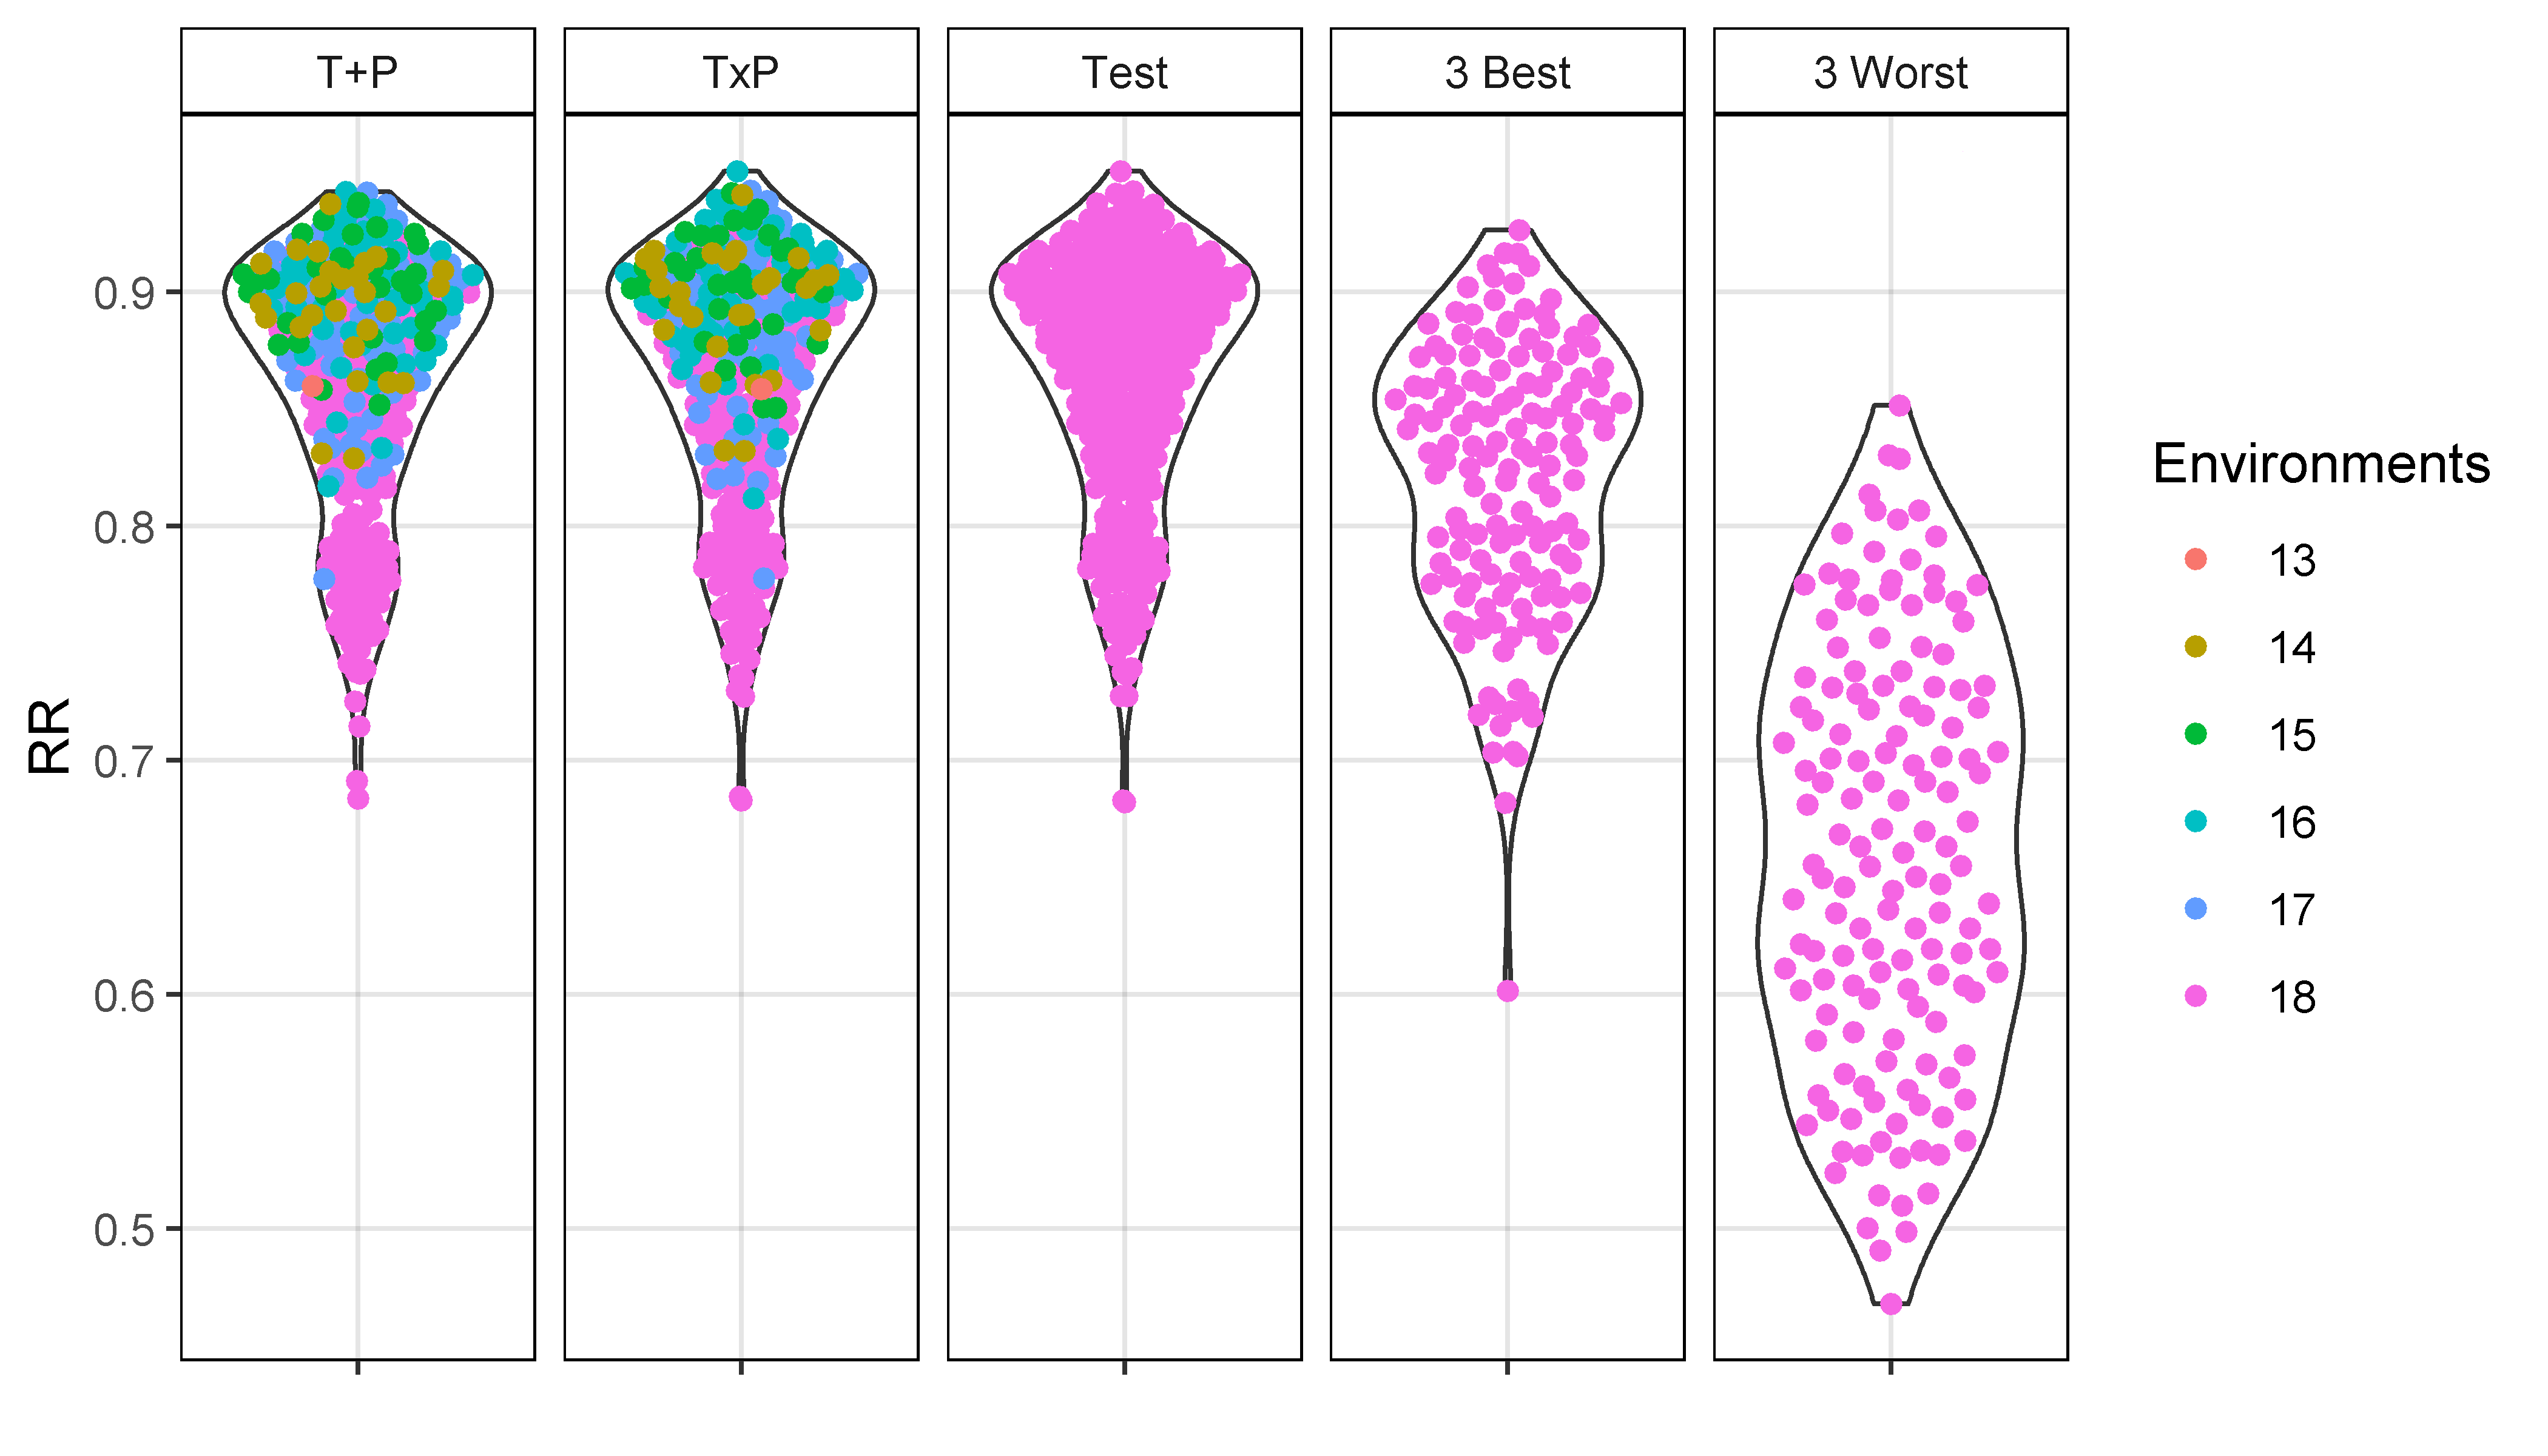
\includegraphics{Additional/Model/Model_pvalues.png}

\begin{Shaded}
\begin{Highlighting}[]
\CommentTok{# Prep data}
\NormalTok{x1 <-}\StringTok{ }\KeywordTok{read.csv}\NormalTok{(}\StringTok{"data/model_t+p_coefs.csv"}\NormalTok{) }\OperatorTok\StringTok{ }\KeywordTok{mutate}\NormalTok{(}\DataTypeTok{Model =} \StringTok{"T+P"}\NormalTok{)}
\NormalTok{x2 <-}\StringTok{ }\KeywordTok{read.csv}\NormalTok{(}\StringTok{"data/model_txp_coefs.csv"}\NormalTok{) }\OperatorTok\StringTok{ }\KeywordTok{mutate}\NormalTok{(}\DataTypeTok{Model =} \StringTok{"TxP"}\NormalTok{)}
\NormalTok{x3 <-}\StringTok{ }\KeywordTok{read.csv}\NormalTok{(}\StringTok{"data/model_test_coefs.csv"}\NormalTok{) }\OperatorTok\StringTok{ }\KeywordTok{mutate}\NormalTok{(}\DataTypeTok{Model =} \StringTok{"Test"}\NormalTok{)}
\NormalTok{x4 <-}\StringTok{ }\KeywordTok{read.csv}\NormalTok{(}\StringTok{"data/model_3best_coefs.csv"}\NormalTok{)  }\OperatorTok\StringTok{ }\KeywordTok{mutate}\NormalTok{(}\DataTypeTok{Model =} \StringTok{"3 Best"}\NormalTok{)}
\NormalTok{x5 <-}\StringTok{ }\KeywordTok{read.csv}\NormalTok{(}\StringTok{"data/model_3worst_coefs.csv"}\NormalTok{)  }\OperatorTok\StringTok{ }\KeywordTok{mutate}\NormalTok{(}\DataTypeTok{Model =} \StringTok{"3 Worst"}\NormalTok{)}
\NormalTok{xx <-}\StringTok{ }\KeywordTok{bind_rows}\NormalTok{(x1, x2, x3, x4, x5) }\OperatorTok\StringTok{ }
\StringTok{  }\KeywordTok{mutate}\NormalTok{(}\DataTypeTok{Model =} \KeywordTok{factor}\NormalTok{(Model, }\DataTypeTok{levels =} \KeywordTok{unique}\NormalTok{(Model)),}
         \DataTypeTok{Environments =} \KeywordTok{factor}\NormalTok{(Environments))}
\CommentTok{# Plot RR}
\NormalTok{mp <-}\StringTok{ }\KeywordTok{ggplot}\NormalTok{(xx, }\KeywordTok{aes}\NormalTok{(}\DataTypeTok{x =} \StringTok{""}\NormalTok{, }\DataTypeTok{y =}\NormalTok{ RR)) }\OperatorTok{+}\StringTok{ }
\StringTok{  }\KeywordTok{geom_violin}\NormalTok{() }\OperatorTok{+}\StringTok{ }\KeywordTok{geom_quasirandom}\NormalTok{(}\KeywordTok{aes}\NormalTok{(}\DataTypeTok{color =}\NormalTok{ Environments)) }\OperatorTok{+}
\StringTok{  }\KeywordTok{facet_grid}\NormalTok{(. }\OperatorTok{~}\StringTok{ }\NormalTok{Model) }\OperatorTok{+}
\StringTok{  }\NormalTok{theme_AGL }\OperatorTok{+}\StringTok{ }
\StringTok{  }\KeywordTok{theme}\NormalTok{(}\DataTypeTok{panel.grid.major.x =} \KeywordTok{element_blank}\NormalTok{()) }\OperatorTok{+}
\StringTok{  }\KeywordTok{labs}\NormalTok{(}\DataTypeTok{x =} \OtherTok{NULL}\NormalTok{)}
\KeywordTok{ggsave}\NormalTok{(}\StringTok{"Additional/Model/Model_pvalues.png"}\NormalTok{, mp, }\DataTypeTok{width =} \DecValTok{7}\NormalTok{, }\DataTypeTok{height =} \DecValTok{4}\NormalTok{, }\DataTypeTok{dpi =} \DecValTok{600}\NormalTok{)}
\end{Highlighting}
\end{Shaded}

\hypertarget{supplemental-figure-6-compare-constants-entry}{%
\subsection{Supplemental Figure 6 Compare Constants
Entry}\label{supplemental-figure-6-compare-constants-entry}}

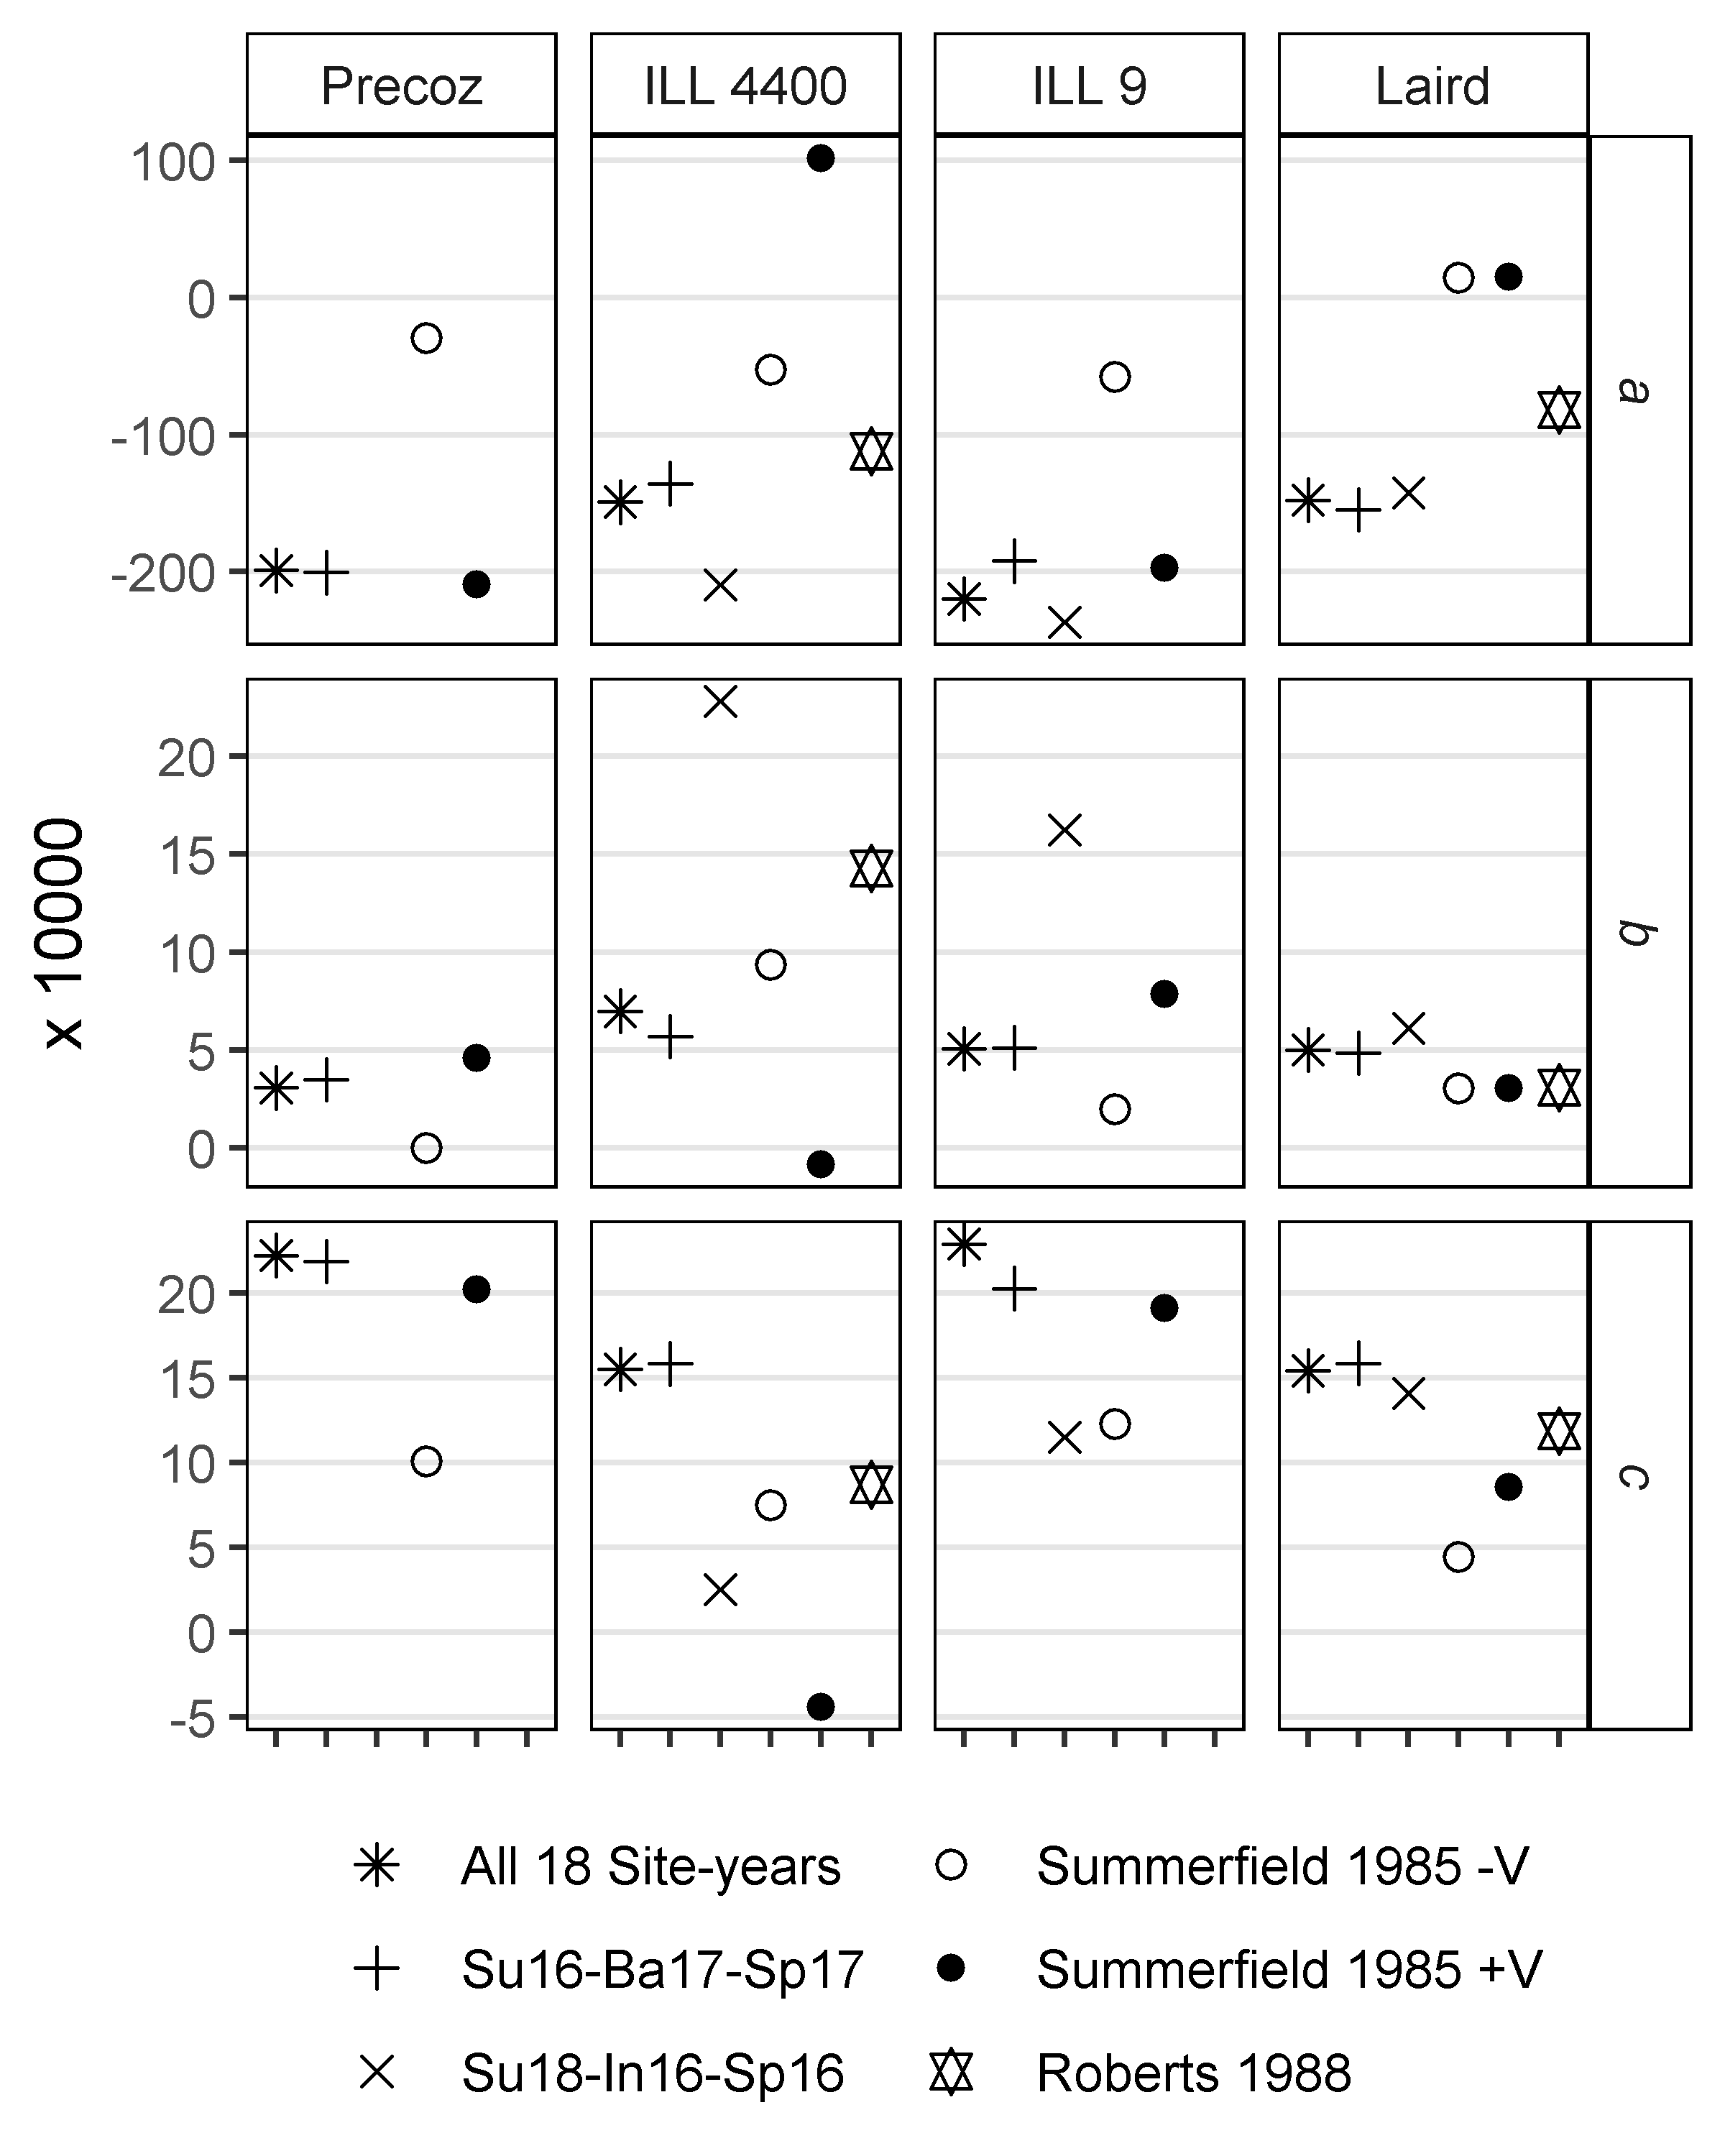
\includegraphics{Supplemental_Figure_06.png}

\begin{itemize}
\tightlist
\item
  Entry 76 = ILL 4400 (Syrian Local Large)
\item
  Entry 77 = ILL 4605 (Precoz)
\item
  Entry 118 = ILL 9
\item
  Entry 128 = Laird
\end{itemize}

\begin{Shaded}
\begin{Highlighting}[]
\CommentTok{# Prep data}
\NormalTok{x1 <-}\StringTok{ }\KeywordTok{read.csv}\NormalTok{(}\StringTok{"data/model_t+p_coefs.csv"}\NormalTok{) }\OperatorTok\StringTok{ }
\StringTok{  }\KeywordTok{filter}\NormalTok{(Entry }\OperatorTok\StringTok{ }\KeywordTok{c}\NormalTok{(}\DecValTok{76}\NormalTok{, }\DecValTok{77}\NormalTok{, }\DecValTok{118}\NormalTok{, }\DecValTok{128}\NormalTok{)) }\OperatorTok\StringTok{ }
\StringTok{  }\KeywordTok{mutate}\NormalTok{(}\DataTypeTok{Expt =} \StringTok{"All 18 Site-years"}\NormalTok{)}
\NormalTok{x2}\FloatTok{.1}\NormalTok{ <-}\StringTok{ }\KeywordTok{read.csv}\NormalTok{(}\StringTok{"data/model_3best_coefs.csv"}\NormalTok{) }\OperatorTok\StringTok{ }
\StringTok{  }\KeywordTok{filter}\NormalTok{(Entry }\OperatorTok\StringTok{ }\KeywordTok{c}\NormalTok{(}\DecValTok{76}\NormalTok{, }\DecValTok{77}\NormalTok{, }\DecValTok{118}\NormalTok{, }\DecValTok{128}\NormalTok{)) }\OperatorTok\StringTok{ }
\StringTok{  }\KeywordTok{mutate}\NormalTok{(}\DataTypeTok{Expt =} \StringTok{"Su16-Ba17-Sp17"}\NormalTok{)}
\NormalTok{x2}\FloatTok{.2}\NormalTok{ <-}\StringTok{ }\KeywordTok{read.csv}\NormalTok{(}\StringTok{"data/model_3worst_coefs.csv"}\NormalTok{) }\OperatorTok\StringTok{ }
\StringTok{  }\KeywordTok{filter}\NormalTok{(Entry }\OperatorTok\StringTok{ }\KeywordTok{c}\NormalTok{(}\DecValTok{76}\NormalTok{, }\DecValTok{77}\NormalTok{, }\DecValTok{118}\NormalTok{, }\DecValTok{128}\NormalTok{)) }\OperatorTok\StringTok{ }
\StringTok{  }\KeywordTok{mutate}\NormalTok{(}\DataTypeTok{Expt =} \StringTok{"Su18-In16-Sp16"}\NormalTok{)}
\CommentTok{# Summerfield et al., 1985}
\NormalTok{x3 <-}\StringTok{ }\NormalTok{x1 }\OperatorTok\StringTok{ }\KeywordTok{mutate}\NormalTok{(}\DataTypeTok{Expt =} \StringTok{"Summerfield 1985 -V"}\NormalTok{)}
\NormalTok{x3[x3}\OperatorTok{$}\NormalTok{Entry }\OperatorTok{==}\StringTok{ }\DecValTok{76}\NormalTok{,  }\KeywordTok{c}\NormalTok{(}\StringTok{"a"}\NormalTok{,}\StringTok{"b"}\NormalTok{,}\StringTok{"c"}\NormalTok{)] <-}\StringTok{ }\KeywordTok{c}\NormalTok{(}\OperatorTok{-}\FloatTok{0.002918}\NormalTok{,  }\DecValTok{0}\NormalTok{,          }\FloatTok{0.0010093}\NormalTok{)}
\NormalTok{x3[x3}\OperatorTok{$}\NormalTok{Entry }\OperatorTok{==}\StringTok{ }\DecValTok{77}\NormalTok{,  }\KeywordTok{c}\NormalTok{(}\StringTok{"a"}\NormalTok{,}\StringTok{"b"}\NormalTok{,}\StringTok{"c"}\NormalTok{)] <-}\StringTok{ }\KeywordTok{c}\NormalTok{(}\OperatorTok{-}\FloatTok{0.0052226}\NormalTok{, }\FloatTok{0.00093643}\NormalTok{, }\FloatTok{0.00075104}\NormalTok{)}
\NormalTok{x3[x3}\OperatorTok{$}\NormalTok{Entry }\OperatorTok{==}\StringTok{ }\DecValTok{118}\NormalTok{, }\KeywordTok{c}\NormalTok{(}\StringTok{"a"}\NormalTok{,}\StringTok{"b"}\NormalTok{,}\StringTok{"c"}\NormalTok{)] <-}\StringTok{ }\KeywordTok{c}\NormalTok{(}\OperatorTok{-}\FloatTok{0.0057408}\NormalTok{, }\FloatTok{0.00020113}\NormalTok{, }\FloatTok{0.0012292}\NormalTok{)}
\NormalTok{x3[x3}\OperatorTok{$}\NormalTok{Entry }\OperatorTok{==}\StringTok{ }\DecValTok{128}\NormalTok{, }\KeywordTok{c}\NormalTok{(}\StringTok{"a"}\NormalTok{,}\StringTok{"b"}\NormalTok{,}\StringTok{"c"}\NormalTok{)] <-}\StringTok{ }\KeywordTok{c}\NormalTok{( }\FloatTok{0.0014689}\NormalTok{, }\FloatTok{0.00030622}\NormalTok{, }\FloatTok{0.00044640}\NormalTok{)}
\NormalTok{x4 <-}\StringTok{ }\NormalTok{x1 }\OperatorTok\StringTok{ }\KeywordTok{mutate}\NormalTok{(}\DataTypeTok{Expt =} \StringTok{"Summerfield 1985 +V"}\NormalTok{)}
\NormalTok{x4[x4}\OperatorTok{$}\NormalTok{Entry }\OperatorTok{==}\StringTok{ }\DecValTok{76}\NormalTok{,  }\KeywordTok{c}\NormalTok{(}\StringTok{"a"}\NormalTok{,}\StringTok{"b"}\NormalTok{,}\StringTok{"c"}\NormalTok{)] <-}\StringTok{ }\KeywordTok{c}\NormalTok{(}\OperatorTok{-}\FloatTok{0.020910}\NormalTok{,   }\FloatTok{0.00045813}\NormalTok{,  }\FloatTok{0.0020210}\NormalTok{)}
\NormalTok{x4[x4}\OperatorTok{$}\NormalTok{Entry }\OperatorTok{==}\StringTok{ }\DecValTok{77}\NormalTok{,  }\KeywordTok{c}\NormalTok{(}\StringTok{"a"}\NormalTok{,}\StringTok{"b"}\NormalTok{,}\StringTok{"c"}\NormalTok{)] <-}\StringTok{ }\KeywordTok{c}\NormalTok{( }\FloatTok{0.0101590}\NormalTok{, }\FloatTok{-0.00008401}\NormalTok{, }\FloatTok{-0.00044067}\NormalTok{)}
\NormalTok{x4[x4}\OperatorTok{$}\NormalTok{Entry }\OperatorTok{==}\StringTok{ }\DecValTok{118}\NormalTok{, }\KeywordTok{c}\NormalTok{(}\StringTok{"a"}\NormalTok{,}\StringTok{"b"}\NormalTok{,}\StringTok{"c"}\NormalTok{)] <-}\StringTok{ }\KeywordTok{c}\NormalTok{(}\OperatorTok{-}\FloatTok{0.0196948}\NormalTok{,  }\FloatTok{0.00078441}\NormalTok{,  }\FloatTok{0.0019110}\NormalTok{)}
\NormalTok{x4[x4}\OperatorTok{$}\NormalTok{Entry }\OperatorTok{==}\StringTok{ }\DecValTok{128}\NormalTok{, }\KeywordTok{c}\NormalTok{(}\StringTok{"a"}\NormalTok{,}\StringTok{"b"}\NormalTok{,}\StringTok{"c"}\NormalTok{)] <-}\StringTok{ }\KeywordTok{c}\NormalTok{( }\FloatTok{0.0015094}\NormalTok{,  }\FloatTok{0.00030622}\NormalTok{,  }\FloatTok{0.00085502}\NormalTok{)}
\CommentTok{# Roberts et al., 1988}
\NormalTok{x5 <-}\StringTok{ }\NormalTok{x1 }\OperatorTok\StringTok{ }\KeywordTok{filter}\NormalTok{(Entry }\OperatorTok\StringTok{ }\KeywordTok{c}\NormalTok{(}\DecValTok{77}\NormalTok{, }\DecValTok{128}\NormalTok{)) }\OperatorTok\StringTok{ }\KeywordTok{mutate}\NormalTok{(}\DataTypeTok{Expt =} \StringTok{"Roberts 1988"}\NormalTok{)}
\NormalTok{x5[x5}\OperatorTok{$}\NormalTok{Entry }\OperatorTok{==}\StringTok{ }\DecValTok{77}\NormalTok{,  }\KeywordTok{c}\NormalTok{(}\StringTok{"a"}\NormalTok{,}\StringTok{"b"}\NormalTok{,}\StringTok{"c"}\NormalTok{)] <-}\StringTok{ }\KeywordTok{c}\NormalTok{(}\OperatorTok{-}\FloatTok{0.0112}\NormalTok{,   }\FloatTok{0.001427}\NormalTok{, }\FloatTok{0.000871}\NormalTok{)}
\NormalTok{x5[x5}\OperatorTok{$}\NormalTok{Entry }\OperatorTok{==}\StringTok{ }\DecValTok{128}\NormalTok{, }\KeywordTok{c}\NormalTok{(}\StringTok{"a"}\NormalTok{,}\StringTok{"b"}\NormalTok{,}\StringTok{"c"}\NormalTok{)] <-}\StringTok{ }\KeywordTok{c}\NormalTok{(}\OperatorTok{-}\FloatTok{0.008172}\NormalTok{, }\FloatTok{0.000309}\NormalTok{, }\FloatTok{0.001187}\NormalTok{)}
\CommentTok{# }
\NormalTok{xx <-}\StringTok{ }\KeywordTok{bind_rows}\NormalTok{(x1, x2}\FloatTok{.1}\NormalTok{, x2}\FloatTok{.2}\NormalTok{, x3, x4, x5) }\OperatorTok
\StringTok{  }\KeywordTok{gather}\NormalTok{(Constant, Value, a, b, c) }\OperatorTok
\StringTok{  }\KeywordTok{mutate}\NormalTok{(}\DataTypeTok{Entry =} \KeywordTok{factor}\NormalTok{(Entry),}
         \DataTypeTok{Name =}\NormalTok{ plyr}\OperatorTok{::}\KeywordTok{mapvalues}\NormalTok{(Entry, }\KeywordTok{c}\NormalTok{(}\DecValTok{76}\NormalTok{,}\DecValTok{77}\NormalTok{,}\DecValTok{118}\NormalTok{,}\DecValTok{128}\NormalTok{), }
                  \KeywordTok{c}\NormalTok{(}\StringTok{"Precoz"}\NormalTok{,}\StringTok{"ILL 4400"}\NormalTok{,}\StringTok{"ILL 9"}\NormalTok{,}\StringTok{"Laird"}\NormalTok{)),}
         \DataTypeTok{Expt =} \KeywordTok{factor}\NormalTok{(Expt, }\DataTypeTok{levels =} \KeywordTok{c}\NormalTok{(}\StringTok{"All 18 Site-years"}\NormalTok{, }
                  \StringTok{"Su16-Ba17-Sp17"}\NormalTok{, }\StringTok{"Su18-In16-Sp16"}\NormalTok{,}
                  \StringTok{"Summerfield 1985 -V"}\NormalTok{, }\StringTok{"Summerfield 1985 +V"}\NormalTok{, }\StringTok{"Roberts 1988"}\NormalTok{)))}
\CommentTok{# Plot}
\NormalTok{mp <-}\StringTok{ }\KeywordTok{ggplot}\NormalTok{(xx, }\KeywordTok{aes}\NormalTok{(}\DataTypeTok{x =}\NormalTok{ Expt, }\DataTypeTok{y =}\NormalTok{ Value }\OperatorTok{*}\StringTok{ }\DecValTok{10000}\NormalTok{, }\DataTypeTok{shape =}\NormalTok{ Expt)) }\OperatorTok{+}\StringTok{ }
\StringTok{  }\KeywordTok{geom_quasirandom}\NormalTok{(}\DataTypeTok{size =} \DecValTok{2}\NormalTok{, }\DataTypeTok{width =} \FloatTok{0.2}\NormalTok{) }\OperatorTok{+}\StringTok{ }
\StringTok{  }\KeywordTok{facet_grid}\NormalTok{(Constant }\OperatorTok{~}\StringTok{ }\NormalTok{Name, }\DataTypeTok{scales =} \StringTok{"free_y"}\NormalTok{) }\OperatorTok{+}
\StringTok{  }\KeywordTok{scale_shape_manual}\NormalTok{(}\DataTypeTok{name =} \OtherTok{NULL}\NormalTok{, }\DataTypeTok{values =} \KeywordTok{c}\NormalTok{(}\DecValTok{8}\NormalTok{,}\DecValTok{3}\NormalTok{,}\DecValTok{4}\NormalTok{,}\DecValTok{1}\NormalTok{,}\DecValTok{16}\NormalTok{,}\DecValTok{11}\NormalTok{)) }\OperatorTok{+}
\StringTok{  }\KeywordTok{guides}\NormalTok{(}\DataTypeTok{shape=}\KeywordTok{guide_legend}\NormalTok{(}\DataTypeTok{nrow =} \DecValTok{3}\NormalTok{, }\DataTypeTok{byrow =}\NormalTok{ F)) }\OperatorTok{+}
\StringTok{  }\NormalTok{theme_AGL }\OperatorTok{+}
\StringTok{  }\KeywordTok{theme}\NormalTok{(}\DataTypeTok{legend.position =} \StringTok{"bottom"}\NormalTok{, }\DataTypeTok{legend.margin =} \KeywordTok{unit}\NormalTok{(}\KeywordTok{c}\NormalTok{(}\DecValTok{0}\NormalTok{,}\DecValTok{0}\NormalTok{,}\DecValTok{0}\NormalTok{,}\DecValTok{0}\NormalTok{), }\StringTok{"cm"}\NormalTok{),}
        \DataTypeTok{strip.text.y =} \KeywordTok{element_text}\NormalTok{(}\DataTypeTok{face =} \StringTok{"italic"}\NormalTok{),}
        \DataTypeTok{panel.grid.major.x =} \KeywordTok{element_blank}\NormalTok{(),}
        \CommentTok{#panel.grid.minor = element_blank(),}
        \DataTypeTok{axis.text.x =} \KeywordTok{element_blank}\NormalTok{()) }\OperatorTok{+}
\StringTok{  }\KeywordTok{labs}\NormalTok{(}\DataTypeTok{x =} \OtherTok{NULL}\NormalTok{, }\DataTypeTok{y =} \StringTok{"x 10000"}\NormalTok{)}
\KeywordTok{ggsave}\NormalTok{(}\StringTok{"Supplemental_Figure_06.png"}\NormalTok{, mp, }\DataTypeTok{width =} \DecValTok{4}\NormalTok{, }\DataTypeTok{height =} \DecValTok{5}\NormalTok{, }\DataTypeTok{dpi =} \DecValTok{600}\NormalTok{)}
\end{Highlighting}
\end{Shaded}

\hypertarget{supplemental-figure-7-3-best-3-worst}{%
\subsection{Supplemental Figure 7 3 best 3
worst}\label{supplemental-figure-7-3-best-3-worst}}

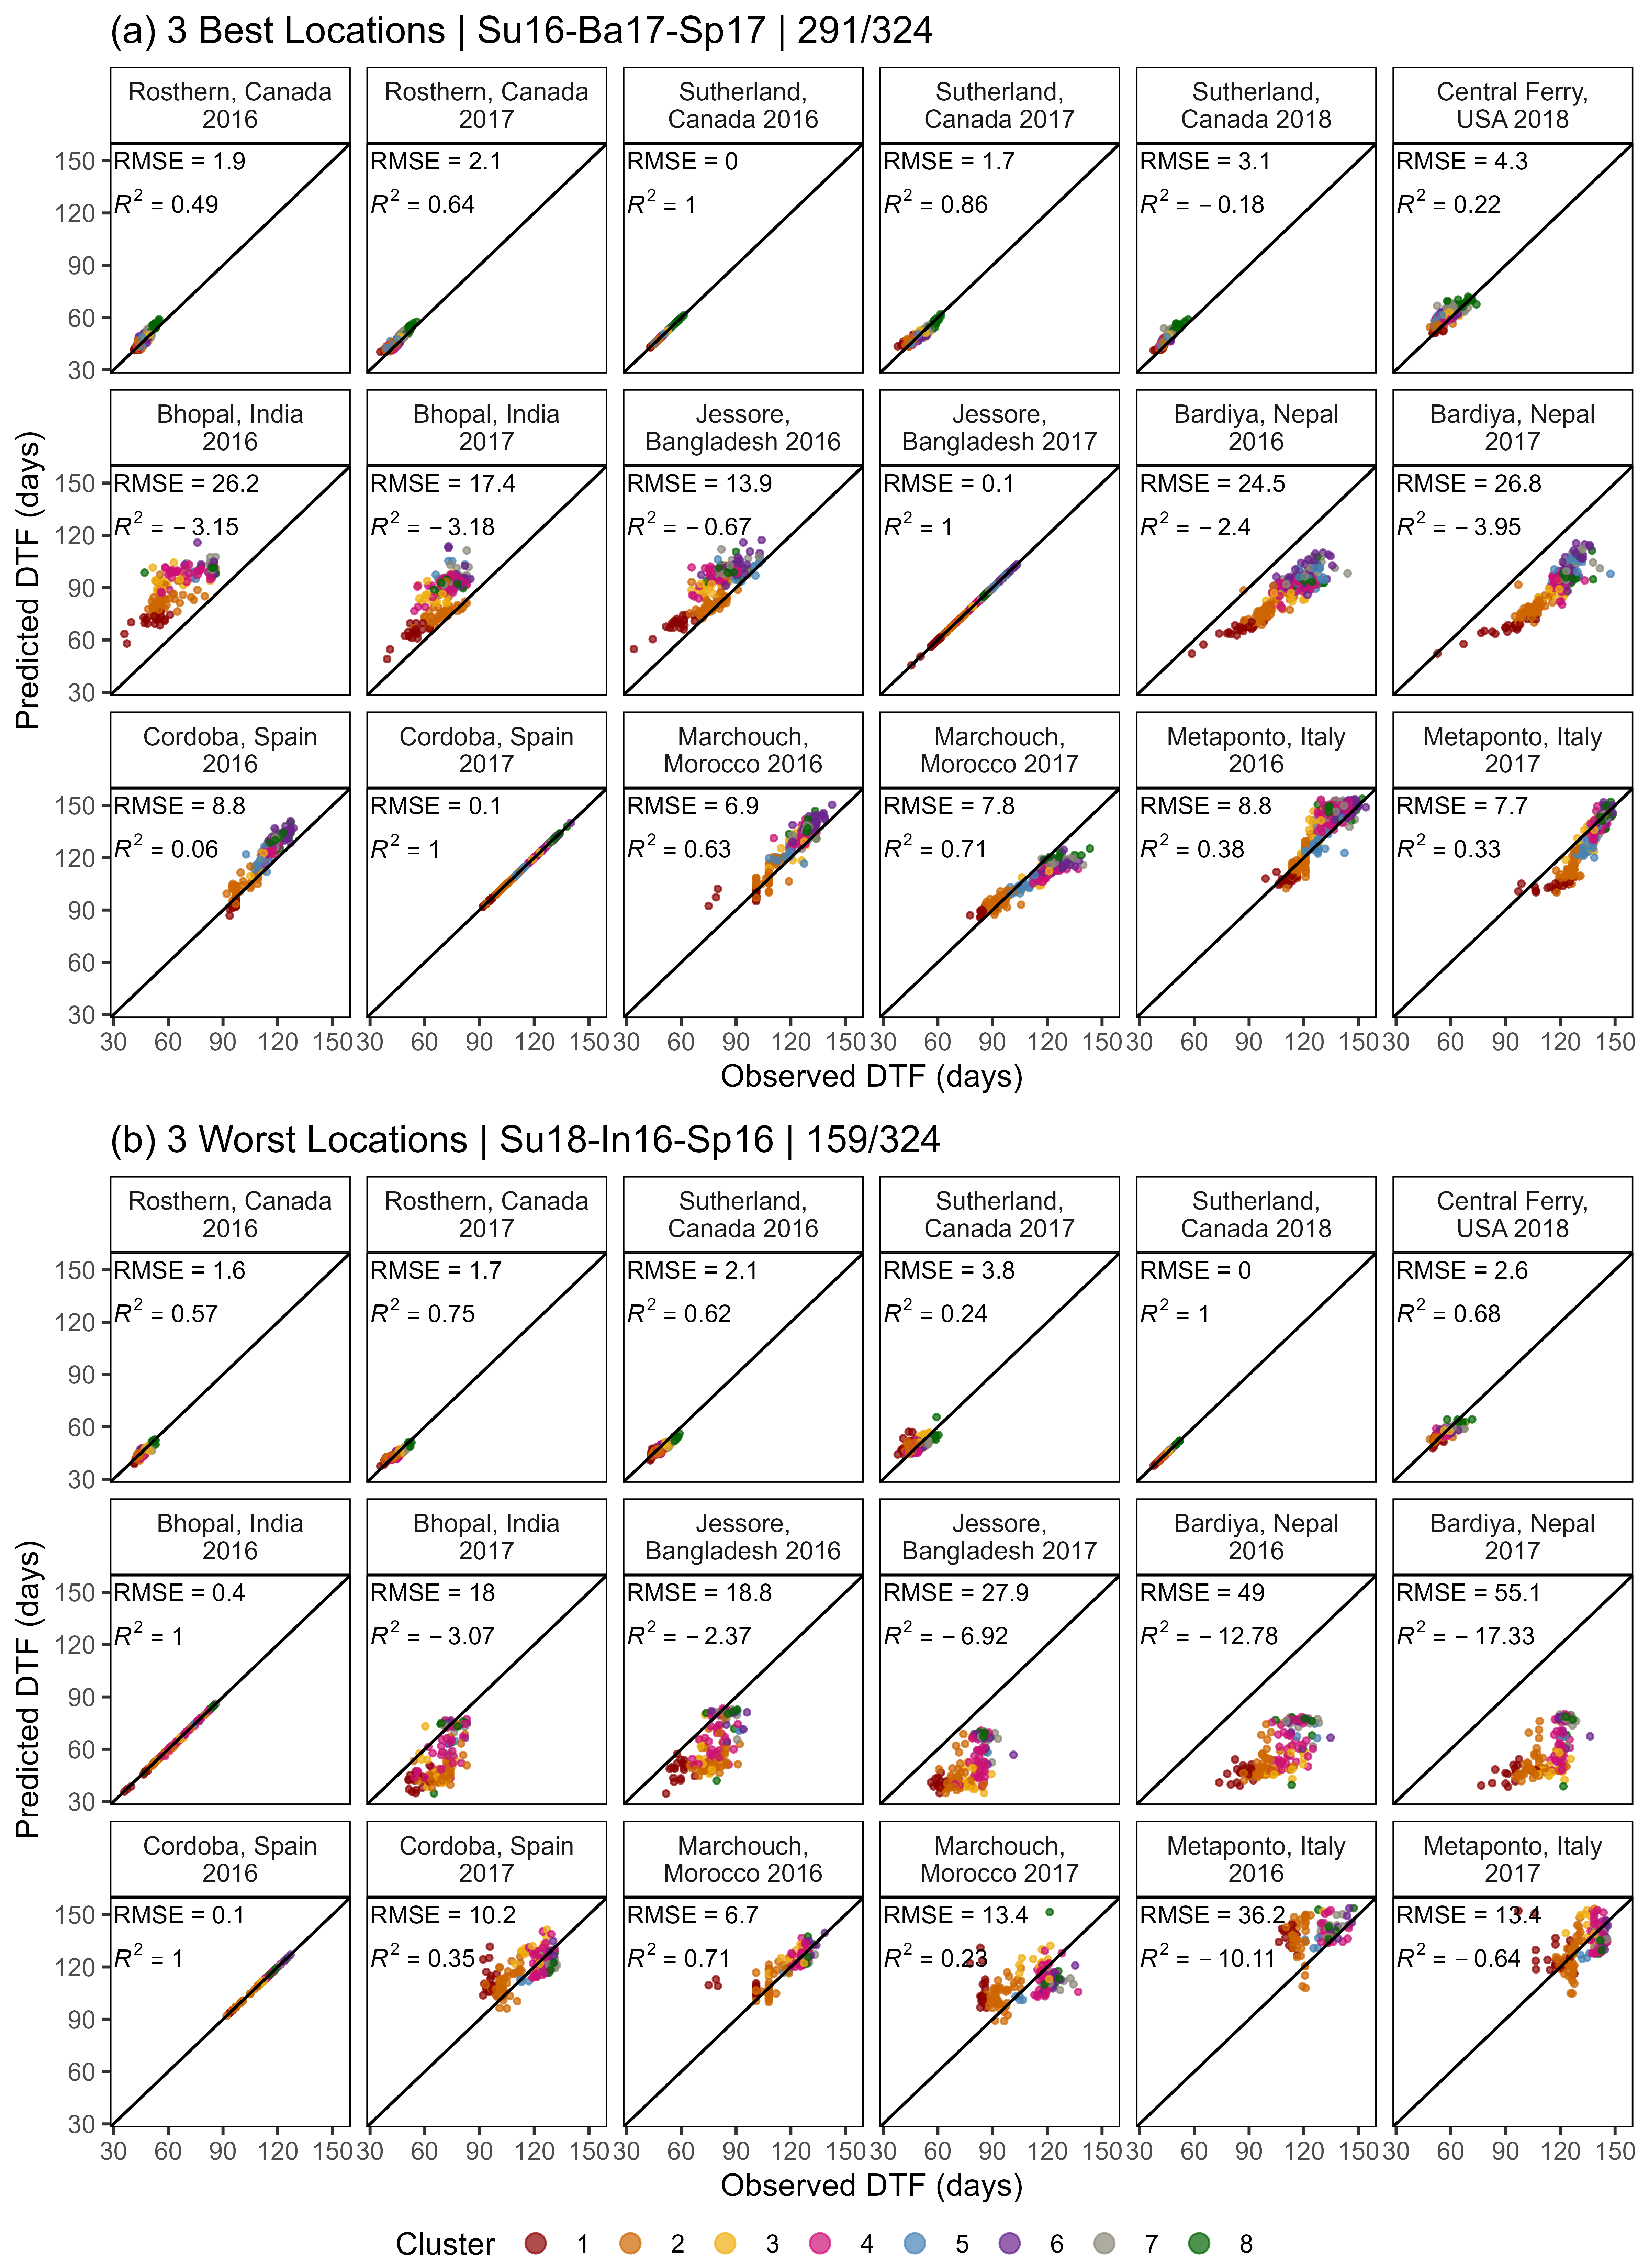
\includegraphics{Supplemental_Figure_07.png}

\begin{Shaded}
\begin{Highlighting}[]
\CommentTok{# Plot (a)}
\NormalTok{xx <-}\StringTok{ }\KeywordTok{read.csv}\NormalTok{(}\StringTok{"data/model_3best_d.csv"}\NormalTok{) }\OperatorTok\StringTok{ }
\StringTok{  }\KeywordTok{mutate}\NormalTok{(}\DataTypeTok{Expt =} \KeywordTok{factor}\NormalTok{(Expt, }\DataTypeTok{levels =}\NormalTok{ names_Expt)) }
\NormalTok{mp1 <-}\StringTok{ }\KeywordTok{gg_model_2}\NormalTok{(xx, }\DataTypeTok{title =} \StringTok{"(a) 3 Best Locations | Su16-Ba17-Sp17 | 291/324"}\NormalTok{)}
\CommentTok{# Plot (b)}
\NormalTok{xx <-}\StringTok{ }\KeywordTok{read.csv}\NormalTok{(}\StringTok{"data/model_3worst_d.csv"}\NormalTok{) }\OperatorTok\StringTok{ }
\StringTok{  }\KeywordTok{mutate}\NormalTok{(}\DataTypeTok{Expt =} \KeywordTok{factor}\NormalTok{(Expt, }\DataTypeTok{levels =}\NormalTok{ names_Expt))}
\NormalTok{mp2 <-}\StringTok{ }\KeywordTok{gg_model_2}\NormalTok{(xx, }\DataTypeTok{title =} \StringTok{"(b) 3 Worst Locations | Su18-In16-Sp16 | 159/324"}\NormalTok{)}
\CommentTok{# Append (a) and (b)}
\NormalTok{mp <-}\StringTok{ }\KeywordTok{ggarrange}\NormalTok{(mp1, mp2, }\DataTypeTok{ncol =} \DecValTok{1}\NormalTok{, }\DataTypeTok{common.legend =}\NormalTok{ T, }\DataTypeTok{legend =} \StringTok{"bottom"}\NormalTok{)}
\KeywordTok{ggsave}\NormalTok{(}\StringTok{"Supplemental_Figure_07.png"}\NormalTok{, mp, }\DataTypeTok{width =} \DecValTok{8}\NormalTok{, }\DataTypeTok{height =} \DecValTok{11}\NormalTok{, }\DataTypeTok{dpi =} \DecValTok{600}\NormalTok{)}
\end{Highlighting}
\end{Shaded}

\hypertarget{supplemental-figure-8-compare-constants-all}{%
\subsection{Supplemental Figure 8 Compare Constants
All}\label{supplemental-figure-8-compare-constants-all}}

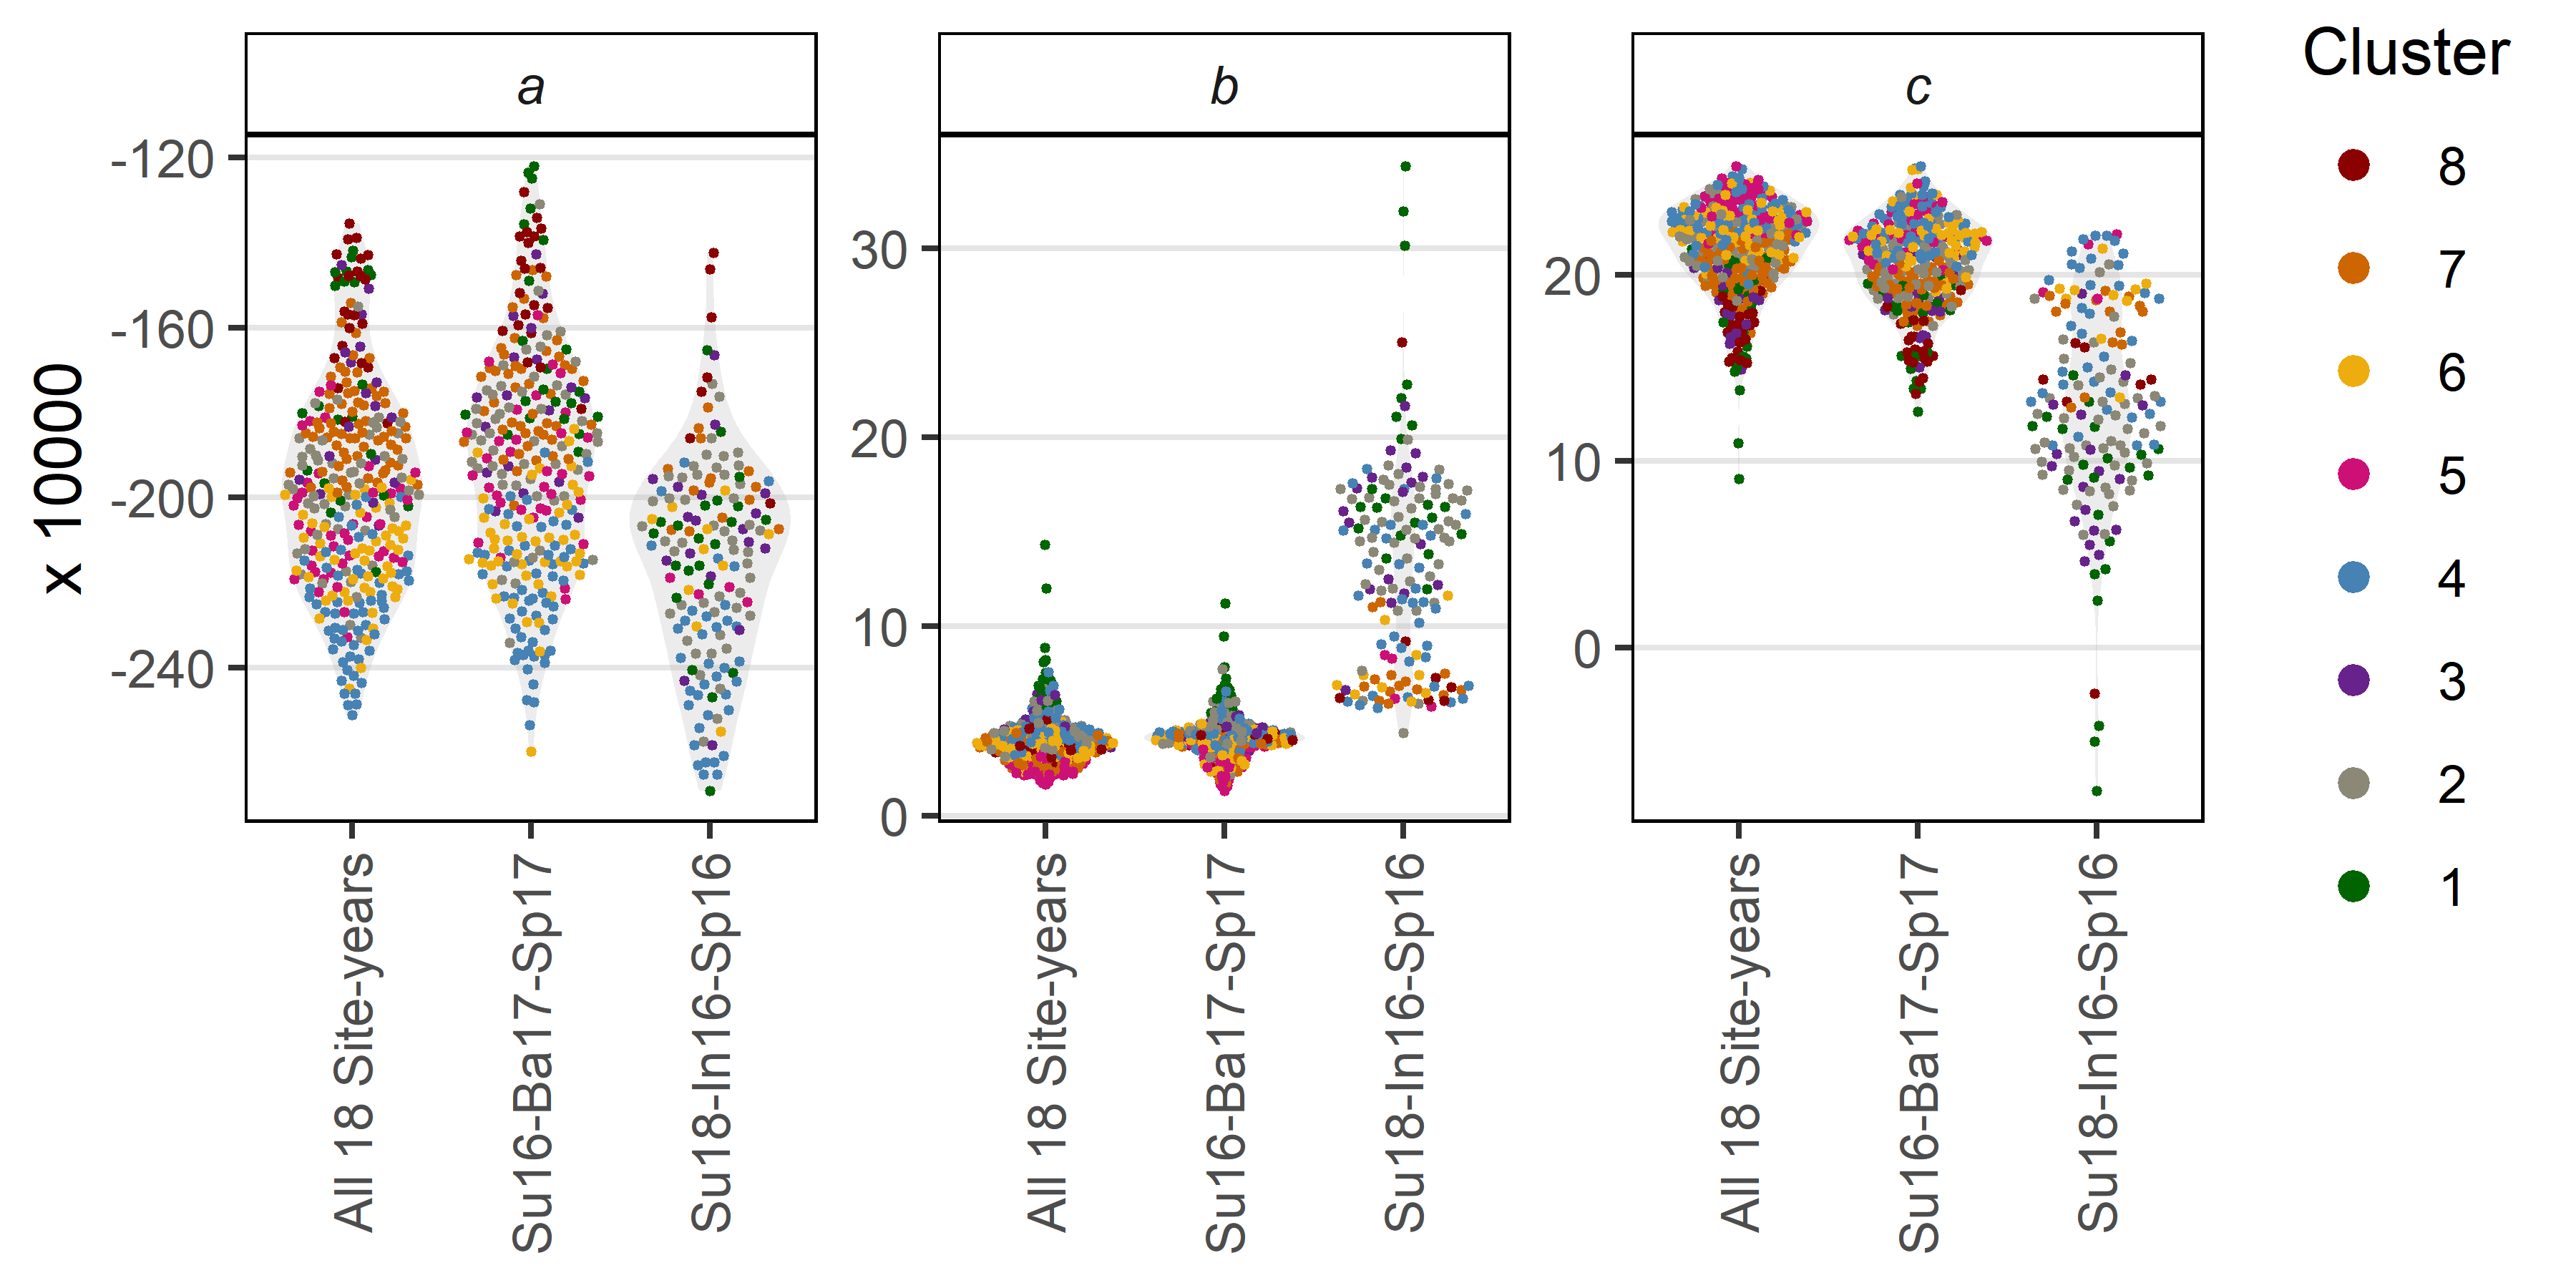
\includegraphics{Supplemental_Figure_08.png}

\begin{Shaded}
\begin{Highlighting}[]
\CommentTok{# Prep data}
\NormalTok{levs <-}\StringTok{ }\KeywordTok{c}\NormalTok{(}\StringTok{"All 18 Site-years"}\NormalTok{, }\StringTok{"Su16-Ba17-Sp17"}\NormalTok{, }\StringTok{"Su18-In16-Sp16"}\NormalTok{)}
\NormalTok{pca <-}\StringTok{ }\KeywordTok{read.csv}\NormalTok{(}\StringTok{"data/data_pca_results.csv"}\NormalTok{) }\OperatorTok\StringTok{ }\KeywordTok{select}\NormalTok{(Entry, Cluster) }\OperatorTok
\StringTok{  }\KeywordTok{mutate}\NormalTok{(}\DataTypeTok{Cluster =} \KeywordTok{factor}\NormalTok{(Cluster))}
\NormalTok{x1 <-}\StringTok{ }\KeywordTok{read.csv}\NormalTok{(}\StringTok{"data/model_t+p_coefs.csv"}\NormalTok{) }\OperatorTok
\StringTok{  }\KeywordTok{mutate}\NormalTok{(}\DataTypeTok{Expt =}\NormalTok{ levs[}\DecValTok{1}\NormalTok{]) }\OperatorTok\StringTok{ }\KeywordTok{select}\NormalTok{(}\OperatorTok{-}\NormalTok{RR)}
\NormalTok{x2 <-}\StringTok{ }\KeywordTok{read.csv}\NormalTok{(}\StringTok{"data/model_3best_coefs.csv"}\NormalTok{) }\OperatorTok\StringTok{ }
\StringTok{  }\KeywordTok{mutate}\NormalTok{(}\DataTypeTok{Expt =}\NormalTok{ levs[}\DecValTok{2}\NormalTok{])}
\NormalTok{x3 <-}\StringTok{ }\KeywordTok{read.csv}\NormalTok{(}\StringTok{"data/model_3worst_coefs.csv"}\NormalTok{) }\OperatorTok\StringTok{ }
\StringTok{  }\KeywordTok{mutate}\NormalTok{(}\DataTypeTok{Expt =}\NormalTok{ levs[}\DecValTok{3}\NormalTok{])}
\NormalTok{xx <-}\StringTok{ }\KeywordTok{bind_rows}\NormalTok{(x1, x2,x3) }\OperatorTok\StringTok{ }
\StringTok{  }\KeywordTok{left_join}\NormalTok{(pca, }\DataTypeTok{by =} \StringTok{"Entry"}\NormalTok{) }\OperatorTok
\StringTok{  }\KeywordTok{gather}\NormalTok{(Trait, Value, a, b, c) }\OperatorTok
\StringTok{  }\KeywordTok{mutate}\NormalTok{(}\DataTypeTok{Expt =} \KeywordTok{factor}\NormalTok{(Expt,}\DataTypeTok{levels =}\NormalTok{ levs))}
\CommentTok{# Plot}
\NormalTok{mp <-}\StringTok{ }\KeywordTok{ggplot}\NormalTok{(xx, }\KeywordTok{aes}\NormalTok{(}\DataTypeTok{x =}\NormalTok{ Expt, }\DataTypeTok{y =}\NormalTok{ Value }\OperatorTok{*}\StringTok{ }\DecValTok{10000}\NormalTok{ )) }\OperatorTok{+}
\StringTok{  }\KeywordTok{geom_violin}\NormalTok{(}\DataTypeTok{alpha =} \FloatTok{0.3}\NormalTok{, }\DataTypeTok{color =} \OtherTok{NA}\NormalTok{, }\DataTypeTok{fill =} \StringTok{"grey"}\NormalTok{) }\OperatorTok{+}\StringTok{ }
\StringTok{  }\KeywordTok{geom_quasirandom}\NormalTok{(}\KeywordTok{aes}\NormalTok{(}\DataTypeTok{color =}\NormalTok{ Cluster), }\DataTypeTok{size =} \FloatTok{0.3}\NormalTok{) }\OperatorTok{+}\StringTok{ }
\StringTok{  }\KeywordTok{facet_wrap}\NormalTok{(Trait }\OperatorTok{~}\StringTok{ }\NormalTok{., }\DataTypeTok{scales =} \StringTok{"free"}\NormalTok{) }\OperatorTok{+}
\StringTok{  }\KeywordTok{scale_color_manual}\NormalTok{(}\DataTypeTok{values =}\NormalTok{ colors, }\DataTypeTok{breaks =} \DecValTok{8}\OperatorTok{:}\DecValTok{1}\NormalTok{) }\OperatorTok{+}
\StringTok{  }\NormalTok{theme_AGL }\OperatorTok{+}
\StringTok{  }\KeywordTok{theme}\NormalTok{(}\DataTypeTok{strip.text =} \KeywordTok{element_text}\NormalTok{(}\DataTypeTok{face =} \StringTok{"italic"}\NormalTok{),}
        \DataTypeTok{panel.grid.major.x =} \KeywordTok{element_blank}\NormalTok{(),}
        \DataTypeTok{axis.text.x =} \KeywordTok{element_text}\NormalTok{(}\DataTypeTok{angle =} \DecValTok{90}\NormalTok{, }\DataTypeTok{vjust =} \FloatTok{0.5}\NormalTok{, }\DataTypeTok{hjust =} \DecValTok{1}\NormalTok{)) }\OperatorTok{+}
\StringTok{  }\KeywordTok{guides}\NormalTok{(}\DataTypeTok{colour =} \KeywordTok{guide_legend}\NormalTok{(}\DataTypeTok{override.aes =} \KeywordTok{list}\NormalTok{(}\DataTypeTok{size =} \DecValTok{2}\NormalTok{))) }\OperatorTok{+}
\StringTok{  }\KeywordTok{labs}\NormalTok{(}\DataTypeTok{x =} \OtherTok{NULL}\NormalTok{, }\DataTypeTok{y =} \StringTok{"x 10000"}\NormalTok{)}
\KeywordTok{ggsave}\NormalTok{(}\StringTok{"Supplemental_Figure_08.png"}\NormalTok{, mp, }\DataTypeTok{width =} \DecValTok{6}\NormalTok{, }\DataTypeTok{height =} \DecValTok{3}\NormalTok{, }\DataTypeTok{dpi =} \DecValTok{600}\NormalTok{)}
\end{Highlighting}
\end{Shaded}

\hypertarget{base-temperature-critical-photoperiod}{%
\subsection{Base Temperature \& Critical
Photoperiod}\label{base-temperature-critical-photoperiod}}

\begin{Shaded}
\begin{Highlighting}[]
\CommentTok{# Calculate Tf and Pf}
\NormalTok{xx <-}\StringTok{ }\KeywordTok{read.csv}\NormalTok{(}\StringTok{"data/model_t+p_coefs.csv"}\NormalTok{) }\OperatorTok\StringTok{ }\KeywordTok{select}\NormalTok{(}\OperatorTok{-}\NormalTok{Name) }\OperatorTok
\StringTok{  }\KeywordTok{mutate}\NormalTok{(}\DataTypeTok{predicted_Tf =} \DecValTok{1}\OperatorTok{/}\NormalTok{b, }\DataTypeTok{predicted_Pf =} \DecValTok{1}\OperatorTok{/}\NormalTok{c )}
\NormalTok{xx <-}\StringTok{ }\NormalTok{rr }\OperatorTok\StringTok{ }\KeywordTok{left_join}\NormalTok{(xx, }\DataTypeTok{by =} \StringTok{"Entry"}\NormalTok{) }\OperatorTok
\StringTok{  }\KeywordTok{left_join}\NormalTok{(}\KeywordTok{select}\NormalTok{(ff, Expt, T_mean, P_mean), }\DataTypeTok{by =} \StringTok{"Expt"}\NormalTok{) }\OperatorTok
\StringTok{  }\KeywordTok{mutate}\NormalTok{(}\DataTypeTok{Tb =} \OperatorTok{-}\NormalTok{(a }\OperatorTok{+}\StringTok{ }\NormalTok{c }\OperatorTok{*}\StringTok{ }\NormalTok{P_mean) }\OperatorTok{/}\StringTok{ }\NormalTok{b,}
         \DataTypeTok{Pc =} \OperatorTok{-}\NormalTok{(a }\OperatorTok{+}\StringTok{ }\NormalTok{b }\OperatorTok{*}\StringTok{ }\NormalTok{T_mean) }\OperatorTok{/}\StringTok{ }\NormalTok{c,}
         \DataTypeTok{Tf_0 =} \OtherTok{NA}\NormalTok{, }\DataTypeTok{Tf_5 =} \OtherTok{NA}\NormalTok{, }\DataTypeTok{Tf =} \OtherTok{NA}\NormalTok{, }\DataTypeTok{Pf =} \OtherTok{NA}\NormalTok{, }\DataTypeTok{PTT =} \OtherTok{NA}\NormalTok{)}
\ControlFlowTok{for}\NormalTok{(i }\ControlFlowTok{in} \DecValTok{1}\OperatorTok{:}\KeywordTok{nrow}\NormalTok{(xx)) \{}
\NormalTok{  e1 <-}\StringTok{ }\NormalTok{ee }\OperatorTok\StringTok{ }\KeywordTok{filter}\NormalTok{(Expt }\OperatorTok{==}\StringTok{ }\NormalTok{xx}\OperatorTok{$}\NormalTok{Expt[i])}
  \ControlFlowTok{for}\NormalTok{(k }\ControlFlowTok{in} \DecValTok{1}\OperatorTok{:}\KeywordTok{nrow}\NormalTok{(e1)) \{ }
\NormalTok{    e1}\OperatorTok{$}\NormalTok{Tfsum[k] <-}\StringTok{ }\KeywordTok{sum}\NormalTok{(e1}\OperatorTok{$}\NormalTok{Temp_mean[}\DecValTok{1}\OperatorTok{:}\NormalTok{k] }\OperatorTok{-}\StringTok{ }\NormalTok{xx}\OperatorTok{$}\NormalTok{Tb[i])}
\NormalTok{    e1}\OperatorTok{$}\NormalTok{Pfsum[k] <-}\StringTok{ }\KeywordTok{sum}\NormalTok{(e1}\OperatorTok{$}\NormalTok{DayLength[}\DecValTok{1}\OperatorTok{:}\NormalTok{k] }\OperatorTok{-}\StringTok{ }\NormalTok{xx}\OperatorTok{$}\NormalTok{Pc[i])}
\NormalTok{  \}}
\NormalTok{  ei <-}\StringTok{ }\NormalTok{e1 }\OperatorTok\StringTok{ }
\StringTok{    }\KeywordTok{filter}\NormalTok{(Date }\OperatorTok{<=}\StringTok{ }\NormalTok{xx}\OperatorTok{$}\NormalTok{PlantingDate[i] }\OperatorTok{+}\StringTok{ }\NormalTok{xx}\OperatorTok{$}\NormalTok{DTF2[i], }\OperatorTok{!}\KeywordTok{is.na}\NormalTok{(Temp_mean)) }
  \ControlFlowTok{if}\NormalTok{(}\KeywordTok{nrow}\NormalTok{(ei) }\OperatorTok{>}\StringTok{ }\DecValTok{0}\NormalTok{) \{}
\NormalTok{    xx}\OperatorTok{$}\NormalTok{Tf_}\DecValTok{0}\NormalTok{[i]  <-}\StringTok{ }\KeywordTok{round}\NormalTok{(}\KeywordTok{sum}\NormalTok{(ei}\OperatorTok{$}\NormalTok{Temp_mean), }\DecValTok{1}\NormalTok{)}
\NormalTok{    xx}\OperatorTok{$}\NormalTok{Tf_}\DecValTok{5}\NormalTok{[i]  <-}\StringTok{ }\KeywordTok{round}\NormalTok{(}\KeywordTok{sum}\NormalTok{(ei}\OperatorTok{$}\NormalTok{Temp_mean }\OperatorTok{-}\StringTok{ }\DecValTok{5}\NormalTok{), }\DecValTok{1}\NormalTok{)}
\NormalTok{    xx}\OperatorTok{$}\NormalTok{Tf[i]    <-}\StringTok{ }\KeywordTok{round}\NormalTok{(}\KeywordTok{sum}\NormalTok{(ei}\OperatorTok{$}\NormalTok{Temp_mean }\OperatorTok{-}\StringTok{ }\NormalTok{xx}\OperatorTok{$}\NormalTok{Tb[i]), }\DecValTok{1}\NormalTok{)}
\NormalTok{    xx}\OperatorTok{$}\NormalTok{Pf_}\DecValTok{0}\NormalTok{[i]  <-}\StringTok{ }\KeywordTok{round}\NormalTok{(}\KeywordTok{sum}\NormalTok{(ei}\OperatorTok{$}\NormalTok{DayLength), }\DecValTok{1}\NormalTok{)}
\NormalTok{    xx}\OperatorTok{$}\NormalTok{Pf_}\DecValTok{7}\NormalTok{[i]  <-}\StringTok{ }\KeywordTok{round}\NormalTok{(}\KeywordTok{sum}\NormalTok{(ei}\OperatorTok{$}\NormalTok{DayLength }\OperatorTok{-}\StringTok{ }\DecValTok{7}\NormalTok{), }\DecValTok{1}\NormalTok{)}
\NormalTok{    xx}\OperatorTok{$}\NormalTok{Pf[i]    <-}\StringTok{ }\KeywordTok{round}\NormalTok{(}\KeywordTok{sum}\NormalTok{(ei}\OperatorTok{$}\NormalTok{DayLength }\OperatorTok{-}\StringTok{ }\NormalTok{xx}\OperatorTok{$}\NormalTok{Pc[i]), }\DecValTok{1}\NormalTok{)}
\NormalTok{    xx}\OperatorTok{$}\NormalTok{PTT_}\DecValTok{0}\NormalTok{[i] <-}\StringTok{ }\KeywordTok{round}\NormalTok{(}\KeywordTok{sum}\NormalTok{(ei}\OperatorTok{$}\NormalTok{Temp_mean }\OperatorTok{*}\StringTok{ }\NormalTok{ei}\OperatorTok{$}\NormalTok{DayLength), }\DecValTok{1}\NormalTok{)}
\NormalTok{    xx}\OperatorTok{$}\NormalTok{PTT[i]   <-}\StringTok{ }\KeywordTok{round}\NormalTok{(}\KeywordTok{sum}\NormalTok{((ei}\OperatorTok{$}\NormalTok{Temp_mean }\OperatorTok{-}\StringTok{ }\NormalTok{xx}\OperatorTok{$}\NormalTok{Tb[i]) }\OperatorTok{*}\StringTok{ }\NormalTok{(ei}\OperatorTok{$}\NormalTok{DayLength }\OperatorTok{-}\StringTok{ }\NormalTok{xx}\OperatorTok{$}\NormalTok{Pc[i])), }\DecValTok{1}\NormalTok{)}
\NormalTok{    eTf <-}\StringTok{ }\NormalTok{e1 }\OperatorTok\StringTok{ }\KeywordTok{filter}\NormalTok{(Tfsum }\OperatorTok{>}\StringTok{ }\NormalTok{xx}\OperatorTok{$}\NormalTok{predicted_Tf[i])}
\NormalTok{    ePf <-}\StringTok{ }\NormalTok{e1 }\OperatorTok\StringTok{ }\KeywordTok{filter}\NormalTok{(Pfsum }\OperatorTok{>}\StringTok{ }\NormalTok{xx}\OperatorTok{$}\NormalTok{predicted_Pf[i])}
\NormalTok{    xx}\OperatorTok{$}\NormalTok{predicted_DTF_Tf[i] <-}\StringTok{ }\NormalTok{eTf}\OperatorTok{$}\NormalTok{DaysAfterPlanting[}\DecValTok{1}\NormalTok{]}
\NormalTok{    xx}\OperatorTok{$}\NormalTok{predicted_DTF_Pf[i] <-}\StringTok{ }\NormalTok{ePf}\OperatorTok{$}\NormalTok{DaysAfterPlanting[}\DecValTok{1}\NormalTok{]}
\NormalTok{  \}}
\NormalTok{\}}
\NormalTok{xx <-}\StringTok{ }\NormalTok{xx }\OperatorTok\StringTok{ }\KeywordTok{left_join}\NormalTok{(}\KeywordTok{select}\NormalTok{(ff, Expt, MacroEnv), }\DataTypeTok{by =} \StringTok{"Expt"}\NormalTok{) }\OperatorTok
\StringTok{  }\KeywordTok{group_by}\NormalTok{(Entry, Name, Expt, ExptShort, MacroEnv) }\OperatorTok\StringTok{ }
\StringTok{  }\KeywordTok{summarise_at}\NormalTok{(}\KeywordTok{vars}\NormalTok{(DTF, Tb, Pc, Tf_}\DecValTok{0}\NormalTok{, Tf_}\DecValTok{5}\NormalTok{, Tf, Pf_}\DecValTok{0}\NormalTok{, Pf_}\DecValTok{7}\NormalTok{, Pf, PTT, PTT_}\DecValTok{0}\NormalTok{,}
\NormalTok{                    predicted_DTF_Tf, predicted_DTF_Pf,}
\NormalTok{                    predicted_Pf, predicted_Tf), }\KeywordTok{funs}\NormalTok{(mean), }\DataTypeTok{na.rm =}\NormalTok{ T) }\OperatorTok
\StringTok{  }\KeywordTok{ungroup}\NormalTok{()}
\CommentTok{# Save}
\KeywordTok{write.csv}\NormalTok{(xx,}\StringTok{"data/data_tb_pc.csv"}\NormalTok{, }\DataTypeTok{row.names =}\NormalTok{ F)}
\end{Highlighting}
\end{Shaded}

\hypertarget{figure-5-tb-and-pc}{%
\subsection{Figure 5 Tb and Pc}\label{figure-5-tb-and-pc}}

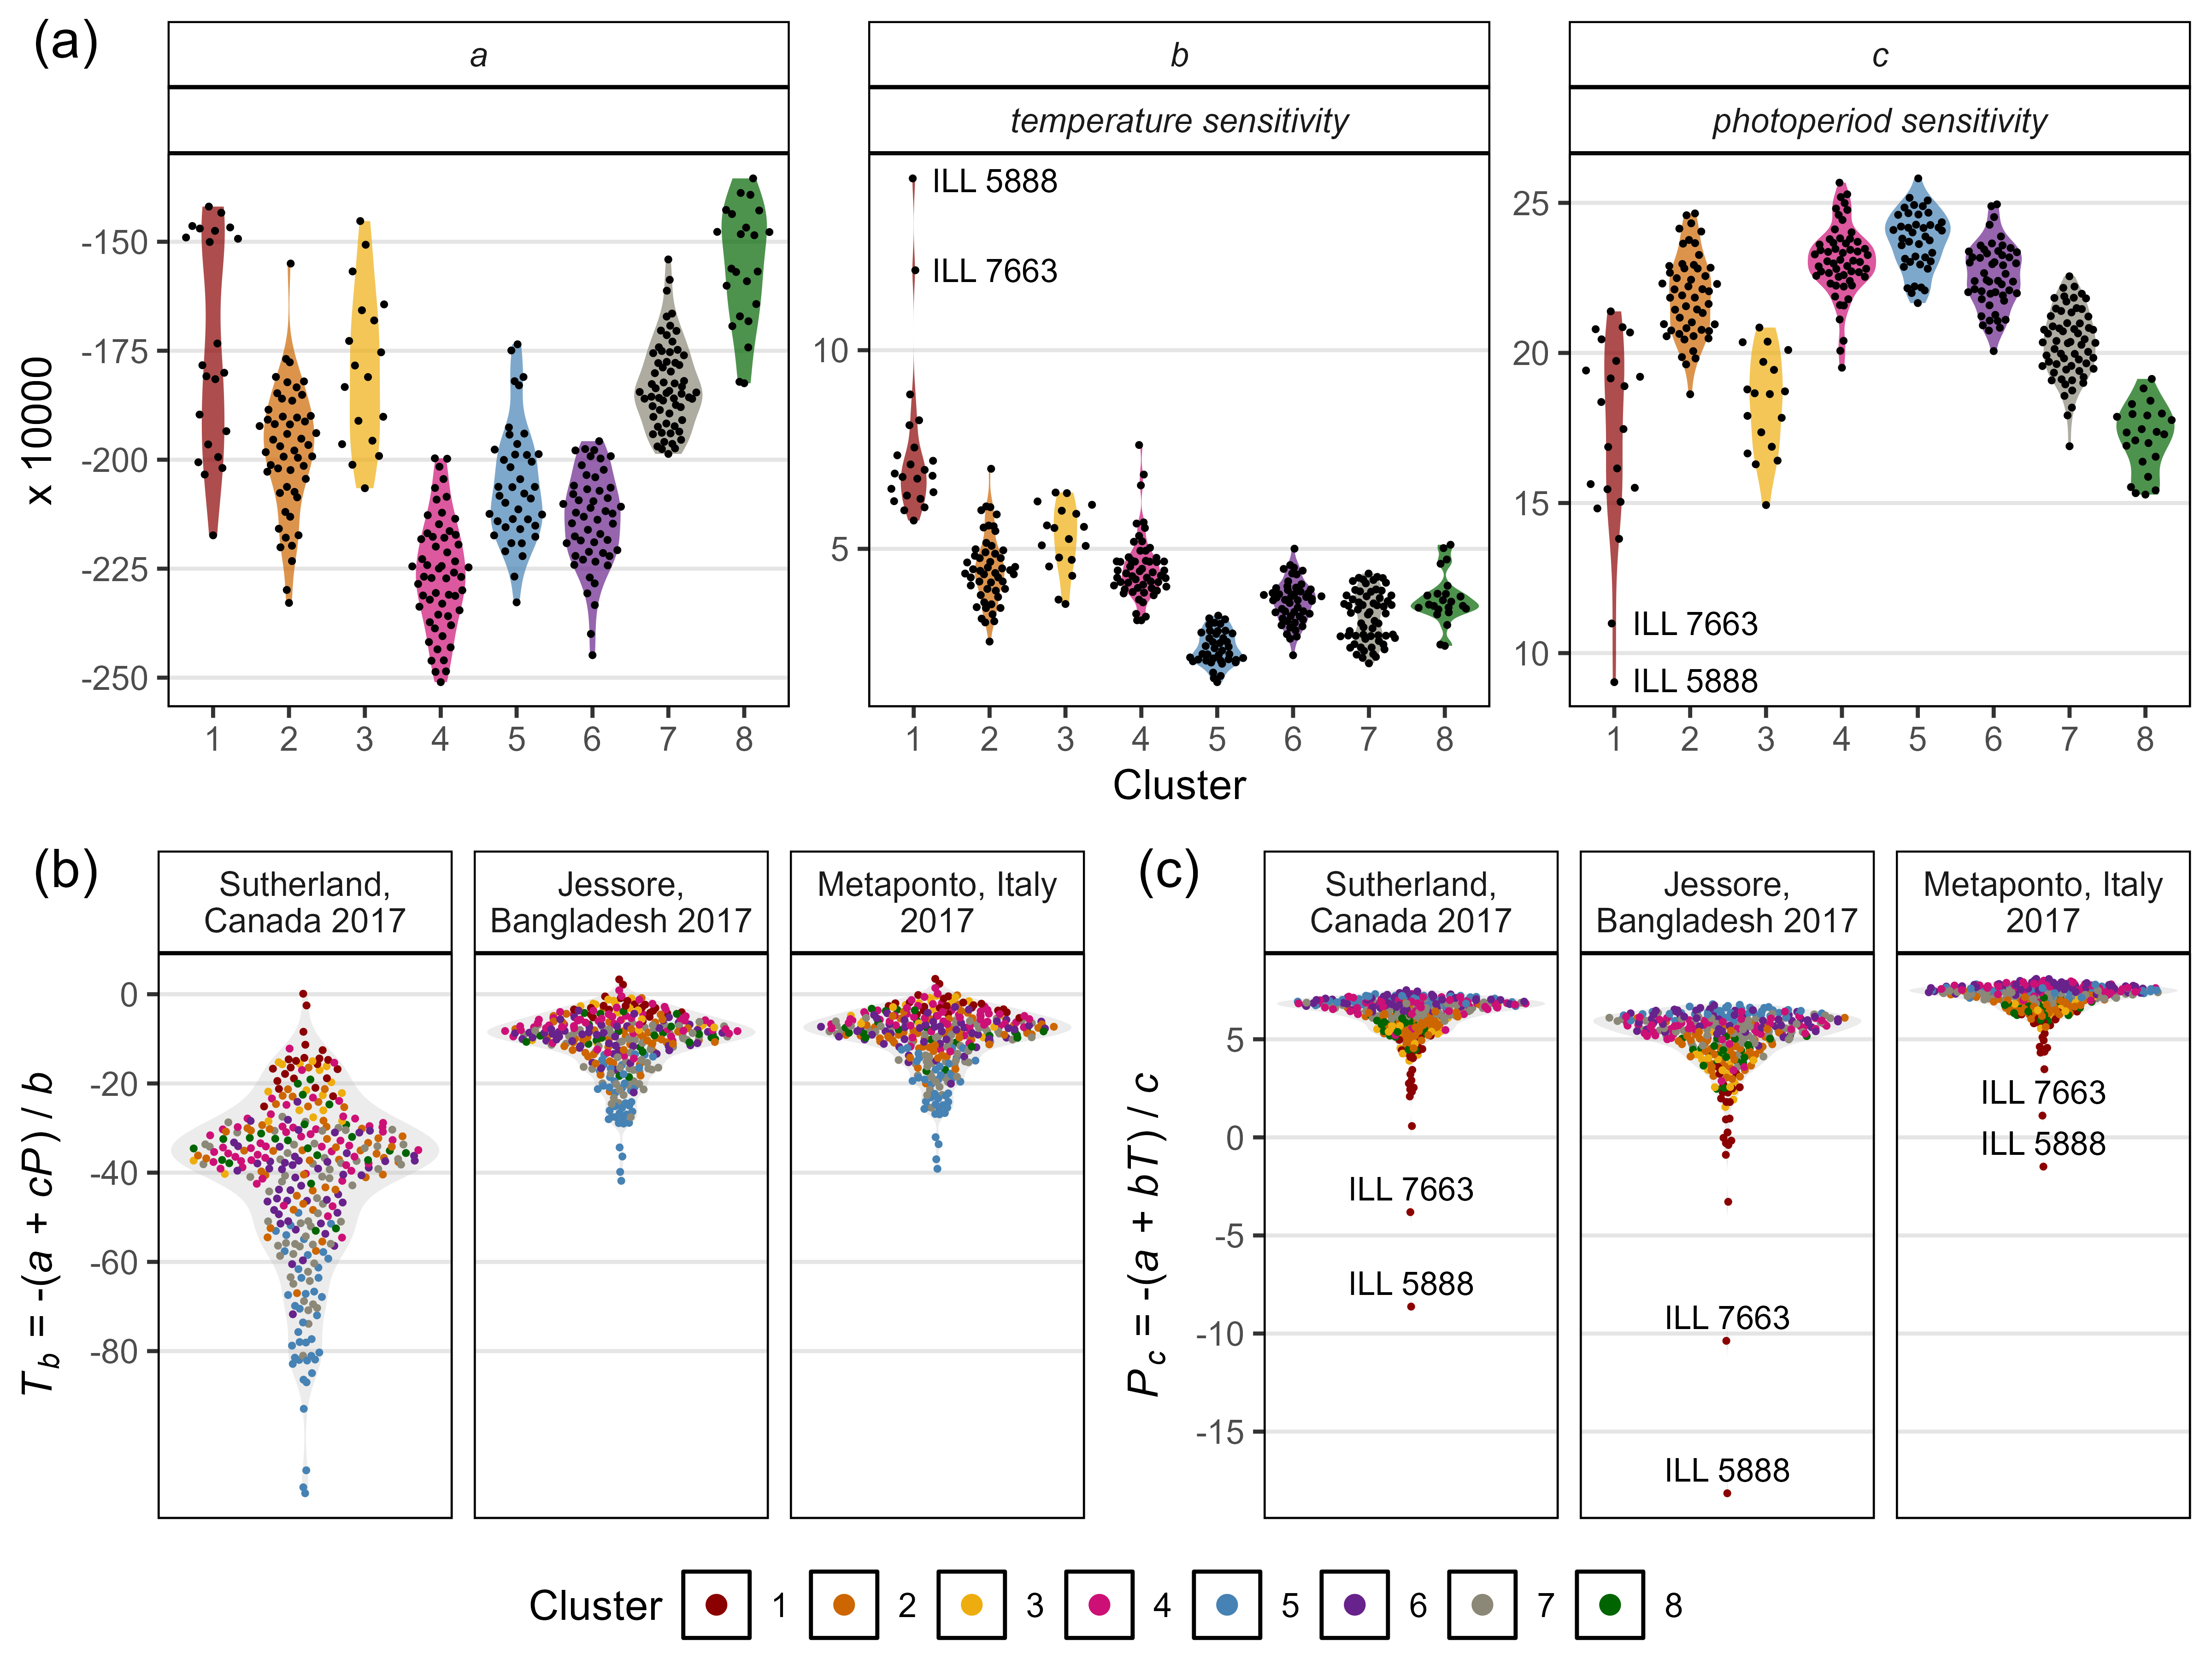
\includegraphics{Figure_05.png}

\begin{Shaded}
\begin{Highlighting}[]
\CommentTok{# Prep data for (a) a, b and c}
\NormalTok{pca <-}\StringTok{ }\KeywordTok{read.csv}\NormalTok{(}\StringTok{"data/data_pca_results.csv"}\NormalTok{) }\OperatorTok\StringTok{ }\KeywordTok{select}\NormalTok{(Entry, Cluster) }\OperatorTok
\StringTok{  }\KeywordTok{mutate}\NormalTok{(}\DataTypeTok{Cluster =} \KeywordTok{factor}\NormalTok{(Cluster))}
\NormalTok{xx <-}\StringTok{ }\KeywordTok{read.csv}\NormalTok{(}\StringTok{"data/model_t+p_coefs.csv"}\NormalTok{) }\OperatorTok
\StringTok{  }\KeywordTok{left_join}\NormalTok{(pca, }\DataTypeTok{by =} \StringTok{"Entry"}\NormalTok{) }\OperatorTok
\StringTok{  }\KeywordTok{select}\NormalTok{(Entry, Name, Cluster, a, b, c) }\OperatorTok
\StringTok{  }\KeywordTok{gather}\NormalTok{(Constant, Value, }\DecValTok{4}\OperatorTok{:}\KeywordTok{ncol}\NormalTok{(.)) }\OperatorTok
\StringTok{  }\KeywordTok{mutate}\NormalTok{(}\DataTypeTok{Meaning =}\NormalTok{ plyr}\OperatorTok{::}\KeywordTok{mapvalues}\NormalTok{(Constant, }\KeywordTok{c}\NormalTok{(}\StringTok{"a"}\NormalTok{,}\StringTok{"b"}\NormalTok{,}\StringTok{"c"}\NormalTok{),}
           \KeywordTok{c}\NormalTok{(}\StringTok{""}\NormalTok{, }\StringTok{"temperature sensitivity"}\NormalTok{, }\StringTok{"photoperiod sensitivity"}\NormalTok{)))}
\NormalTok{x1 <-}\StringTok{ }\NormalTok{xx }\OperatorTok\StringTok{ }\KeywordTok{filter}\NormalTok{(Entry }\OperatorTok\StringTok{ }\KeywordTok{c}\NormalTok{(}\DecValTok{94}\NormalTok{,}\DecValTok{105}\NormalTok{), Constant }\OperatorTok{!=}\StringTok{ "a"}\NormalTok{) }\OperatorTok\StringTok{ }
\StringTok{  }\KeywordTok{mutate}\NormalTok{(}\DataTypeTok{Name =} \KeywordTok{gsub}\NormalTok{(}\StringTok{" AGL"}\NormalTok{, }\StringTok{""}\NormalTok{, Name))}
\CommentTok{# Plot (a) a, b and c}
\NormalTok{mp1 <-}\StringTok{ }\KeywordTok{ggplot}\NormalTok{(xx, }\KeywordTok{aes}\NormalTok{(}\DataTypeTok{x =}\NormalTok{ Cluster, }\DataTypeTok{y =}\NormalTok{ Value }\OperatorTok{*}\StringTok{ }\DecValTok{10000}\NormalTok{) ) }\OperatorTok{+}\StringTok{ }
\StringTok{  }\KeywordTok{geom_violin}\NormalTok{(}\KeywordTok{aes}\NormalTok{(}\DataTypeTok{fill =}\NormalTok{ Cluster), }\DataTypeTok{color =} \OtherTok{NA}\NormalTok{, }\DataTypeTok{alpha =} \FloatTok{0.7}\NormalTok{) }\OperatorTok{+}\StringTok{ }
\StringTok{  }\KeywordTok{geom_quasirandom}\NormalTok{(}\DataTypeTok{size =} \FloatTok{0.3}\NormalTok{) }\OperatorTok{+}\StringTok{ }
\StringTok{  }\KeywordTok{geom_text_repel}\NormalTok{(}\DataTypeTok{data =}\NormalTok{ x1, }\KeywordTok{aes}\NormalTok{(}\DataTypeTok{label =}\NormalTok{ Name), }\DataTypeTok{size =} \DecValTok{3}\NormalTok{, }\DataTypeTok{nudge_x =} \FloatTok{0.5}\NormalTok{) }\OperatorTok{+}
\StringTok{  }\KeywordTok{facet_wrap}\NormalTok{(Constant}\OperatorTok{+}\NormalTok{Meaning }\OperatorTok{~}\StringTok{ }\NormalTok{., }\DataTypeTok{nrow =} \DecValTok{1}\NormalTok{, }\DataTypeTok{scales =} \StringTok{"free"}\NormalTok{) }\OperatorTok{+}\StringTok{ }
\StringTok{  }\NormalTok{theme_AGL }\OperatorTok{+}
\StringTok{  }\KeywordTok{theme}\NormalTok{(}\DataTypeTok{strip.text =} \KeywordTok{element_text}\NormalTok{(}\DataTypeTok{face =} \StringTok{"italic"}\NormalTok{),}
        \DataTypeTok{legend.position =} \StringTok{"none"}\NormalTok{, }\DataTypeTok{panel.grid.major.x =} \KeywordTok{element_blank}\NormalTok{()) }\OperatorTok{+}
\StringTok{  }\KeywordTok{scale_fill_manual}\NormalTok{(}\DataTypeTok{name =} \OtherTok{NULL}\NormalTok{, }\DataTypeTok{values =}\NormalTok{ colors) }\OperatorTok{+}
\StringTok{  }\KeywordTok{guides}\NormalTok{(}\DataTypeTok{fill =}\NormalTok{ F) }\OperatorTok{+}
\StringTok{  }\KeywordTok{labs}\NormalTok{(}\DataTypeTok{y =} \StringTok{"x 10000"}\NormalTok{)}
\CommentTok{# Prep data}
\NormalTok{xx <-}\StringTok{ }\KeywordTok{read.csv}\NormalTok{(}\StringTok{"data/data_tb_pc.csv"}\NormalTok{) }\OperatorTok\StringTok{ }
\StringTok{  }\KeywordTok{left_join}\NormalTok{(pca, }\DataTypeTok{by =} \StringTok{"Entry"}\NormalTok{) }\OperatorTok
\StringTok{  }\KeywordTok{mutate}\NormalTok{(}\DataTypeTok{Expt =} \KeywordTok{factor}\NormalTok{(Expt, }\DataTypeTok{levels =}\NormalTok{ names_Expt)) }\OperatorTok
\StringTok{  }\KeywordTok{select}\NormalTok{(Entry, Name, Expt, ExptShort, Cluster, Tb, Pc, predicted_Tf, predicted_Pf)}
\NormalTok{x1 <-}\StringTok{ }\NormalTok{xx }\OperatorTok\StringTok{ }
\StringTok{  }\KeywordTok{filter}\NormalTok{(ExptShort }\OperatorTok\StringTok{ }\KeywordTok{c}\NormalTok{(}\StringTok{"Su17"}\NormalTok{, }\StringTok{"Ba17"}\NormalTok{, }\StringTok{"It17"}\NormalTok{)) }\OperatorTok\StringTok{ }
\StringTok{  }\KeywordTok{group_by}\NormalTok{(Entry, Name, Expt, ExptShort, Cluster) }\OperatorTok
\StringTok{  }\KeywordTok{summarise_at}\NormalTok{(}\KeywordTok{vars}\NormalTok{(Tb, Pc), }\KeywordTok{funs}\NormalTok{(mean), }\DataTypeTok{na.rm =}\NormalTok{ T) }
\CommentTok{# Plot (b) Tb}
\NormalTok{mp2}\FloatTok{.1}\NormalTok{ <-}\StringTok{ }\KeywordTok{ggplot}\NormalTok{(x1, }\KeywordTok{aes}\NormalTok{(}\DataTypeTok{x =} \DecValTok{1}\NormalTok{, }\DataTypeTok{y =}\NormalTok{ Tb)) }\OperatorTok{+}\StringTok{ }
\StringTok{  }\KeywordTok{geom_violin}\NormalTok{(}\DataTypeTok{fill =} \StringTok{"grey"}\NormalTok{, }\DataTypeTok{alpha =} \FloatTok{0.3}\NormalTok{, }\DataTypeTok{color =} \OtherTok{NA}\NormalTok{) }\OperatorTok{+}\StringTok{ }
\StringTok{  }\KeywordTok{geom_quasirandom}\NormalTok{(}\KeywordTok{aes}\NormalTok{(}\DataTypeTok{color =}\NormalTok{ Cluster), }\DataTypeTok{size =} \FloatTok{0.3}\NormalTok{) }\OperatorTok{+}\StringTok{ }
\StringTok{  }\KeywordTok{facet_grid}\NormalTok{(. }\OperatorTok{~}\StringTok{ }\NormalTok{Expt, }\DataTypeTok{labeller =} \KeywordTok{label_wrap_gen}\NormalTok{(}\DataTypeTok{width =} \DecValTok{17}\NormalTok{)) }\OperatorTok{+}
\StringTok{  }\KeywordTok{scale_y_continuous}\NormalTok{(}\DataTypeTok{breaks =} \KeywordTok{seq}\NormalTok{(}\OperatorTok{-}\DecValTok{80}\NormalTok{,}\DecValTok{0}\NormalTok{,}\DecValTok{20}\NormalTok{), }\DataTypeTok{minor_breaks =} \KeywordTok{seq}\NormalTok{(}\OperatorTok{-}\DecValTok{110}\NormalTok{,}\DecValTok{0}\NormalTok{,}\DecValTok{10}\NormalTok{)) }\OperatorTok{+}
\StringTok{  }\KeywordTok{scale_color_manual}\NormalTok{(}\DataTypeTok{values =}\NormalTok{ colors) }\OperatorTok{+}
\StringTok{  }\NormalTok{theme_AGL }\OperatorTok{+}
\StringTok{  }\KeywordTok{theme}\NormalTok{(}\DataTypeTok{axis.text.x  =} \KeywordTok{element_blank}\NormalTok{(), }
        \DataTypeTok{axis.ticks.x =} \KeywordTok{element_blank}\NormalTok{(),}
        \DataTypeTok{panel.grid.major.x =} \KeywordTok{element_blank}\NormalTok{()) }\OperatorTok{+}
\StringTok{  }\KeywordTok{guides}\NormalTok{(}\DataTypeTok{colour =} \KeywordTok{guide_legend}\NormalTok{(}\DataTypeTok{nrow =} \DecValTok{1}\NormalTok{, }\DataTypeTok{override.aes =} \KeywordTok{list}\NormalTok{(}\DataTypeTok{size=}\DecValTok{2}\NormalTok{))) }\OperatorTok{+}
\StringTok{  }\KeywordTok{labs}\NormalTok{(}\DataTypeTok{y =} \KeywordTok{expression}\NormalTok{(}\KeywordTok{paste}\NormalTok{(}\KeywordTok{italic}\NormalTok{(}\StringTok{"T"}\NormalTok{)[}\KeywordTok{italic}\NormalTok{(}\StringTok{"b"}\NormalTok{)], }\StringTok{" = -("}\NormalTok{, }\KeywordTok{italic}\NormalTok{(}\StringTok{"a"}\NormalTok{), }\StringTok{" + "}\NormalTok{,}
              \KeywordTok{italic}\NormalTok{(}\StringTok{"cP"}\NormalTok{), }\StringTok{") / "}\NormalTok{, }\KeywordTok{italic}\NormalTok{(}\StringTok{"b"}\NormalTok{))), }\DataTypeTok{x =} \OtherTok{NULL}\NormalTok{)}
\CommentTok{# Plot (c) Pc}
\NormalTok{x2 <-}\StringTok{ }\NormalTok{x1 }\OperatorTok\StringTok{ }\KeywordTok{filter}\NormalTok{(Entry }\OperatorTok\StringTok{ }\KeywordTok{c}\NormalTok{(}\DecValTok{94}\NormalTok{,}\DecValTok{105}\NormalTok{)) }\OperatorTok
\StringTok{  }\KeywordTok{ungroup}\NormalTok{() }\OperatorTok\StringTok{ }\KeywordTok{mutate}\NormalTok{(}\DataTypeTok{Name =} \KeywordTok{gsub}\NormalTok{(}\StringTok{" AGL"}\NormalTok{, }\StringTok{""}\NormalTok{, Name))}
\NormalTok{mp2}\FloatTok{.2}\NormalTok{ <-}\StringTok{ }\KeywordTok{ggplot}\NormalTok{(x1, }\KeywordTok{aes}\NormalTok{(}\DataTypeTok{x =} \DecValTok{1}\NormalTok{, }\DataTypeTok{y =}\NormalTok{ Pc)) }\OperatorTok{+}\StringTok{ }
\StringTok{  }\KeywordTok{geom_violin}\NormalTok{(}\DataTypeTok{fill =} \StringTok{"grey"}\NormalTok{, }\DataTypeTok{alpha =} \FloatTok{0.3}\NormalTok{, }\DataTypeTok{color =} \OtherTok{NA}\NormalTok{) }\OperatorTok{+}\StringTok{ }
\StringTok{  }\KeywordTok{geom_quasirandom}\NormalTok{(}\KeywordTok{aes}\NormalTok{(}\DataTypeTok{color =}\NormalTok{ Cluster), }\DataTypeTok{size =} \FloatTok{0.3}\NormalTok{) }\OperatorTok{+}\StringTok{ }
\StringTok{  }\KeywordTok{facet_grid}\NormalTok{(. }\OperatorTok{~}\StringTok{ }\NormalTok{Expt, }\DataTypeTok{labeller =} \KeywordTok{label_wrap_gen}\NormalTok{(}\DataTypeTok{width =} \DecValTok{17}\NormalTok{)) }\OperatorTok{+}
\StringTok{  }\KeywordTok{geom_text}\NormalTok{(}\DataTypeTok{data =}\NormalTok{ x2, }\KeywordTok{aes}\NormalTok{(}\DataTypeTok{label =}\NormalTok{ Name), }\DataTypeTok{size =} \DecValTok{3}\NormalTok{, }\DataTypeTok{nudge_y =} \FloatTok{1.2}\NormalTok{) }\OperatorTok{+}
\StringTok{  }\KeywordTok{scale_y_continuous}\NormalTok{(}\DataTypeTok{breaks =} \KeywordTok{c}\NormalTok{(}\OperatorTok{-}\DecValTok{20}\NormalTok{,}\OperatorTok{-}\DecValTok{15}\NormalTok{,}\OperatorTok{-}\DecValTok{10}\NormalTok{,}\OperatorTok{-}\DecValTok{5}\NormalTok{,}\DecValTok{0}\NormalTok{,}\DecValTok{5}\NormalTok{)) }\OperatorTok{+}
\StringTok{  }\KeywordTok{scale_color_manual}\NormalTok{(}\DataTypeTok{values =}\NormalTok{ colors) }\OperatorTok{+}
\StringTok{  }\NormalTok{theme_AGL }\OperatorTok{+}
\StringTok{  }\KeywordTok{theme}\NormalTok{(}\DataTypeTok{axis.text.x        =} \KeywordTok{element_blank}\NormalTok{(),}
        \DataTypeTok{axis.ticks.x       =} \KeywordTok{element_blank}\NormalTok{(),}
        \DataTypeTok{panel.grid.major.x =} \KeywordTok{element_blank}\NormalTok{()) }\OperatorTok{+}
\StringTok{  }\KeywordTok{guides}\NormalTok{(}\DataTypeTok{colour =} \KeywordTok{guide_legend}\NormalTok{(}\DataTypeTok{nrow =} \DecValTok{1}\NormalTok{, }\DataTypeTok{override.aes =} \KeywordTok{list}\NormalTok{(}\DataTypeTok{size=}\DecValTok{2}\NormalTok{))) }\OperatorTok{+}
\StringTok{  }\KeywordTok{labs}\NormalTok{(}\DataTypeTok{y =} \KeywordTok{expression}\NormalTok{(}\KeywordTok{paste}\NormalTok{(}\KeywordTok{italic}\NormalTok{(}\StringTok{"P"}\NormalTok{)[}\KeywordTok{italic}\NormalTok{(}\StringTok{"c"}\NormalTok{)], }\StringTok{" = -("}\NormalTok{, }\KeywordTok{italic}\NormalTok{(}\StringTok{"a"}\NormalTok{), }\StringTok{" + "}\NormalTok{, }
             \KeywordTok{italic}\NormalTok{(}\StringTok{"bT"}\NormalTok{), }\StringTok{") / "}\NormalTok{, }\KeywordTok{italic}\NormalTok{(}\StringTok{"c"}\NormalTok{))), }\DataTypeTok{x =} \OtherTok{NULL}\NormalTok{)}
\NormalTok{mp2 <-}\StringTok{ }\KeywordTok{ggarrange}\NormalTok{(mp2}\FloatTok{.1}\NormalTok{, mp2}\FloatTok{.2}\NormalTok{, }\DataTypeTok{nrow =} \DecValTok{1}\NormalTok{, }\DataTypeTok{ncol =} \DecValTok{2}\NormalTok{, }\DataTypeTok{common.legend =}\NormalTok{ T, }\DataTypeTok{legend =} \StringTok{"bottom"}\NormalTok{,}
                 \DataTypeTok{labels =} \KeywordTok{c}\NormalTok{(}\StringTok{"(b)"}\NormalTok{,}\StringTok{"(c)"}\NormalTok{), }\DataTypeTok{font.label =} \KeywordTok{list}\NormalTok{(}\DataTypeTok{face =} \StringTok{"plain"}\NormalTok{))}
\CommentTok{#}
\NormalTok{mp <-}\StringTok{ }\KeywordTok{ggarrange}\NormalTok{(mp1, mp2, }\DataTypeTok{nrow =} \DecValTok{2}\NormalTok{, }\DataTypeTok{ncol =} \DecValTok{1}\NormalTok{, }\DataTypeTok{align =} \StringTok{"hv"}\NormalTok{, }
                \DataTypeTok{labels =} \KeywordTok{c}\NormalTok{(}\StringTok{"(a)"}\NormalTok{,}\StringTok{""}\NormalTok{), }\DataTypeTok{font.label =} \KeywordTok{list}\NormalTok{(}\DataTypeTok{face =} \StringTok{"plain"}\NormalTok{)) }\CommentTok{#heights = }
\KeywordTok{ggsave}\NormalTok{(}\StringTok{"Figure_05.png"}\NormalTok{, mp, }\DataTypeTok{width =} \DecValTok{8}\NormalTok{, }\DataTypeTok{height =} \DecValTok{6}\NormalTok{, }\DataTypeTok{dpi =} \DecValTok{600}\NormalTok{)}
\end{Highlighting}
\end{Shaded}

\hypertarget{figure-6-origin-constants}{%
\subsection{Figure 6 Origin Constants}\label{figure-6-origin-constants}}

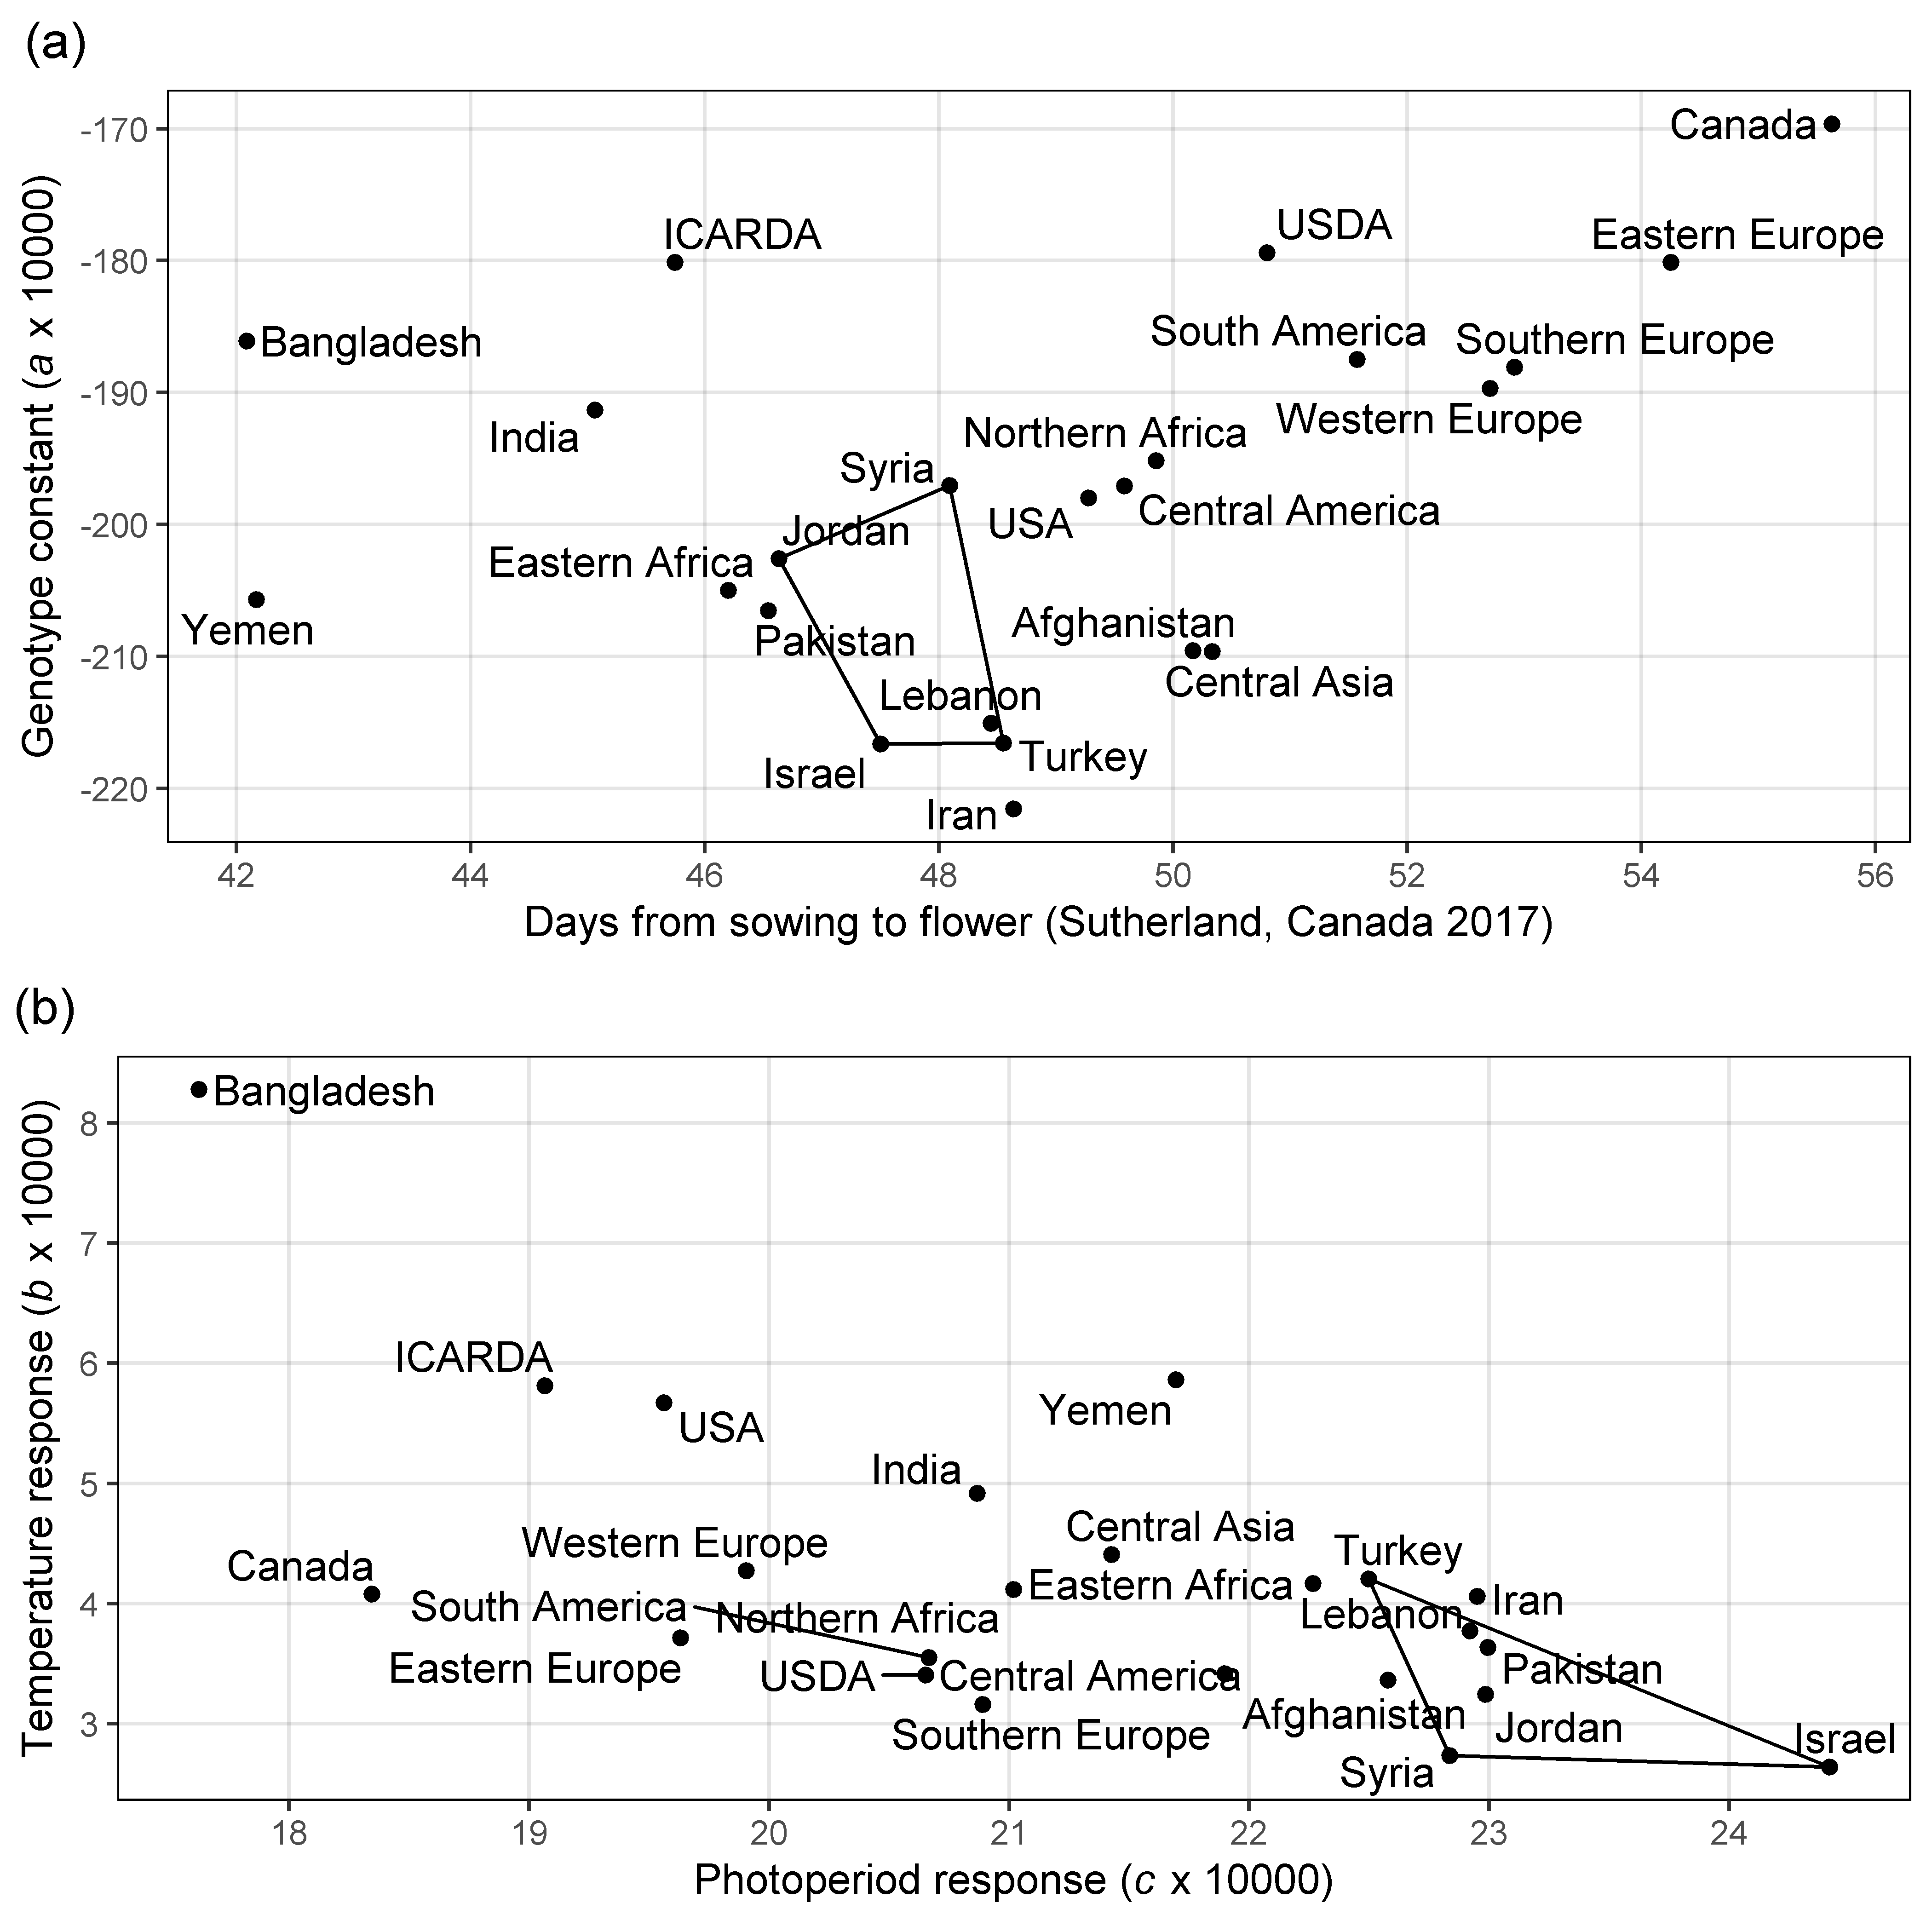
\includegraphics{Figure_06.png}

\begin{Shaded}
\begin{Highlighting}[]
\CommentTok{# Prep data}
\NormalTok{mycts <-}\StringTok{ }\KeywordTok{c}\NormalTok{(}\StringTok{"Canada"}\NormalTok{, }\StringTok{"USA"}\NormalTok{, }\StringTok{"Iran"}\NormalTok{, }\StringTok{"Yemen"}\NormalTok{,}
           \StringTok{"India"}\NormalTok{, }\StringTok{"Pakistan"}\NormalTok{, }\StringTok{"Bangladesh"}\NormalTok{, }\StringTok{"Afghanistan"}\NormalTok{,}
           \StringTok{"Syria"}\NormalTok{, }\StringTok{"Jordan"}\NormalTok{, }\StringTok{"Turkey"}\NormalTok{, }\StringTok{"Lebanon"}\NormalTok{, }\StringTok{"Israel"}\NormalTok{)}
\NormalTok{xx <-}\StringTok{ }\KeywordTok{read.csv}\NormalTok{(}\StringTok{"data/model_t+p_coefs.csv"}\NormalTok{) }\OperatorTok\StringTok{ }
\StringTok{  }\KeywordTok{left_join}\NormalTok{(}\KeywordTok{select}\NormalTok{(ldp, Entry, Origin), }\DataTypeTok{by =} \StringTok{"Entry"}\NormalTok{) }\OperatorTok
\StringTok{  }\KeywordTok{left_join}\NormalTok{(}\KeywordTok{select}\NormalTok{(ct, }\DataTypeTok{Origin=}\NormalTok{Country, SubRegion), }\DataTypeTok{by =} \StringTok{"Origin"}\NormalTok{) }\OperatorTok
\StringTok{  }\KeywordTok{filter}\NormalTok{(Origin }\OperatorTok{!=}\StringTok{ "Unknown"}\NormalTok{) }\OperatorTok
\StringTok{  }\KeywordTok{mutate}\NormalTok{(}\DataTypeTok{SubRegion =} \KeywordTok{as.character}\NormalTok{(SubRegion), }\DataTypeTok{Origin =} \KeywordTok{as.character}\NormalTok{(Origin),}
         \DataTypeTok{SubRegion =} \KeywordTok{ifelse}\NormalTok{(Origin }\OperatorTok\StringTok{ }\KeywordTok{c}\NormalTok{(}\StringTok{"ICARDA"}\NormalTok{, }\StringTok{"USDA"}\NormalTok{), }
\NormalTok{                            Origin, }\KeywordTok{as.character}\NormalTok{(SubRegion)),}
         \DataTypeTok{Origin =} \KeywordTok{ifelse}\NormalTok{(Origin }\OperatorTok\StringTok{ }\NormalTok{mycts, Origin, }\KeywordTok{as.character}\NormalTok{(SubRegion)))}
\NormalTok{x1 <-}\StringTok{ }\NormalTok{xx }\OperatorTok\StringTok{ }
\StringTok{  }\KeywordTok{left_join}\NormalTok{(dd }\OperatorTok\StringTok{ }\KeywordTok{filter}\NormalTok{(ExptShort }\OperatorTok{==}\StringTok{ "Su17"}\NormalTok{) }\OperatorTok\StringTok{ }\KeywordTok{select}\NormalTok{(Entry, DTF), }\DataTypeTok{by =} \StringTok{"Entry"}\NormalTok{) }\OperatorTok
\StringTok{  }\KeywordTok{group_by}\NormalTok{(Origin) }\OperatorTok\StringTok{ }
\StringTok{  }\KeywordTok{summarise_at}\NormalTok{(}\KeywordTok{vars}\NormalTok{(DTF, a, b, c), }\KeywordTok{funs}\NormalTok{(mean, sd)) }\OperatorTok\StringTok{ }
\StringTok{  }\KeywordTok{filter}\NormalTok{(Origin }\OperatorTok{!=}\StringTok{ "Unknown"}\NormalTok{)}
\NormalTok{x2 <-}\StringTok{ }\NormalTok{x1 }\OperatorTok\StringTok{ }\KeywordTok{mutate}\NormalTok{(}\DataTypeTok{CO =} \DecValTok{1}\NormalTok{) }\OperatorTok
\StringTok{  }\KeywordTok{filter}\NormalTok{(Origin }\OperatorTok\StringTok{ }\KeywordTok{c}\NormalTok{(}\StringTok{"Syria"}\NormalTok{, }\StringTok{"Jordan"}\NormalTok{, }\StringTok{"Turkey"}\NormalTok{, }\StringTok{"Lebanon"}\NormalTok{, }\StringTok{"Israel"}\NormalTok{))}
\CommentTok{# Plot (a) a vs DTF}
\NormalTok{find_hull <-}\StringTok{ }\ControlFlowTok{function}\NormalTok{(df) df[}\KeywordTok{chull}\NormalTok{(df[,}\StringTok{"DTF_mean"}\NormalTok{], df[,}\StringTok{"a_mean"}\NormalTok{]), ]}
\NormalTok{polys <-}\StringTok{ }\NormalTok{plyr}\OperatorTok{::}\KeywordTok{ddply}\NormalTok{(x2, }\StringTok{"CO"}\NormalTok{, find_hull)}
\NormalTok{mp1 <-}\StringTok{ }\KeywordTok{ggplot}\NormalTok{(x1, }\KeywordTok{aes}\NormalTok{(}\DataTypeTok{x =}\NormalTok{ DTF_mean, }\DataTypeTok{y =}\NormalTok{ a_mean }\OperatorTok{*}\StringTok{ }\DecValTok{10000}\NormalTok{)) }\OperatorTok{+}\StringTok{ }
\StringTok{  }\KeywordTok{geom_polygon}\NormalTok{(}\DataTypeTok{data =}\NormalTok{ polys, }\DataTypeTok{fill =} \OtherTok{NA}\NormalTok{, }\DataTypeTok{color =} \StringTok{"black"}\NormalTok{) }\OperatorTok{+}
\StringTok{  }\KeywordTok{geom_point}\NormalTok{() }\OperatorTok{+}\StringTok{ }\KeywordTok{geom_text_repel}\NormalTok{(}\KeywordTok{aes}\NormalTok{(}\DataTypeTok{label =}\NormalTok{ Origin)) }\OperatorTok{+}
\StringTok{  }\KeywordTok{scale_x_continuous}\NormalTok{(}\DataTypeTok{breaks =} \KeywordTok{seq}\NormalTok{(}\DecValTok{42}\NormalTok{, }\DecValTok{56}\NormalTok{, }\DecValTok{2}\NormalTok{)) }\OperatorTok{+}\StringTok{ }
\StringTok{  }\NormalTok{theme_AGL }\OperatorTok{+}
\StringTok{  }\KeywordTok{theme}\NormalTok{(}\DataTypeTok{plot.title =} \KeywordTok{element_text}\NormalTok{(}\DataTypeTok{hjust =} \FloatTok{-0.085}\NormalTok{) ) }\OperatorTok{+}
\StringTok{  }\KeywordTok{labs}\NormalTok{(}\DataTypeTok{title =} \StringTok{"(a)"}\NormalTok{,}
       \DataTypeTok{y =} \KeywordTok{expression}\NormalTok{(}\KeywordTok{paste}\NormalTok{(}\StringTok{"Genotype constant ("}\NormalTok{, }\KeywordTok{italic}\NormalTok{(a),}\StringTok{" x 10000)"}\NormalTok{)), }
       \DataTypeTok{x =} \StringTok{"Days from sowing to flower (Sutherland, Canada 2017)"}\NormalTok{)}
\CommentTok{# Plot (b) b vs c}
\NormalTok{find_hull <-}\StringTok{ }\ControlFlowTok{function}\NormalTok{(df) df[}\KeywordTok{chull}\NormalTok{(df[,}\StringTok{"c_mean"}\NormalTok{], df[,}\StringTok{"b_mean"}\NormalTok{]), ]}
\NormalTok{polys <-}\StringTok{ }\NormalTok{plyr}\OperatorTok{::}\KeywordTok{ddply}\NormalTok{(x2, }\StringTok{"CO"}\NormalTok{, find_hull)}
\NormalTok{mp2 <-}\StringTok{ }\KeywordTok{ggplot}\NormalTok{(x1, }\KeywordTok{aes}\NormalTok{(}\DataTypeTok{x =}\NormalTok{ c_mean }\OperatorTok{*}\StringTok{ }\DecValTok{10000}\NormalTok{, }\DataTypeTok{y =}\NormalTok{ b_mean }\OperatorTok{*}\StringTok{ }\DecValTok{10000}\NormalTok{)) }\OperatorTok{+}\StringTok{ }
\StringTok{  }\KeywordTok{geom_polygon}\NormalTok{(}\DataTypeTok{data =}\NormalTok{ polys, }\DataTypeTok{fill =} \OtherTok{NA}\NormalTok{, }\DataTypeTok{color =} \StringTok{"black"}\NormalTok{) }\OperatorTok{+}
\StringTok{  }\KeywordTok{geom_point}\NormalTok{() }\OperatorTok{+}\StringTok{ }\KeywordTok{geom_text_repel}\NormalTok{(}\KeywordTok{aes}\NormalTok{(}\DataTypeTok{label =}\NormalTok{ Origin)) }\OperatorTok{+}
\StringTok{  }\KeywordTok{scale_x_continuous}\NormalTok{(}\DataTypeTok{breaks =} \KeywordTok{seq}\NormalTok{(}\DecValTok{18}\NormalTok{, }\DecValTok{24}\NormalTok{, }\DecValTok{1}\NormalTok{)) }\OperatorTok{+}
\StringTok{  }\KeywordTok{scale_y_continuous}\NormalTok{(}\DataTypeTok{breaks =} \DecValTok{3}\OperatorTok{:}\DecValTok{8}\NormalTok{) }\OperatorTok{+}
\StringTok{  }\NormalTok{theme_AGL }\OperatorTok{+}
\StringTok{  }\KeywordTok{theme}\NormalTok{(}\DataTypeTok{plot.title =} \KeywordTok{element_text}\NormalTok{(}\DataTypeTok{hjust =} \FloatTok{-0.06}\NormalTok{) ) }\OperatorTok{+}
\StringTok{  }\KeywordTok{labs}\NormalTok{(}\DataTypeTok{title =} \StringTok{"(b)"}\NormalTok{,}
       \DataTypeTok{y =} \KeywordTok{expression}\NormalTok{(}\KeywordTok{paste}\NormalTok{(}\StringTok{"Temperature response ("}\NormalTok{, }\KeywordTok{italic}\NormalTok{(b), }\StringTok{" x 10000)"}\NormalTok{)), }
       \DataTypeTok{x =} \KeywordTok{expression}\NormalTok{(}\KeywordTok{paste}\NormalTok{(}\StringTok{"Photoperiod response ("}\NormalTok{, }\KeywordTok{italic}\NormalTok{(c), }\StringTok{" x 10000)"}\NormalTok{)))}
\CommentTok{# Append (a) and (b)}
\NormalTok{mp <-}\StringTok{ }\KeywordTok{ggarrange}\NormalTok{(mp1, mp2, }\DataTypeTok{ncol =} \DecValTok{1}\NormalTok{, }\DataTypeTok{nrow =} \DecValTok{2}\NormalTok{)}
\KeywordTok{ggsave}\NormalTok{(}\StringTok{"Figure_06.png"}\NormalTok{, mp, }\DataTypeTok{width =} \DecValTok{7}\NormalTok{, }\DataTypeTok{height =} \DecValTok{7}\NormalTok{, }\DataTypeTok{dpi =} \DecValTok{600}\NormalTok{)}
\KeywordTok{ggsave}\NormalTok{(}\StringTok{"Additional/Temp/Temp_F06_1.png"}\NormalTok{, mp1, }\DataTypeTok{width =} \DecValTok{8}\NormalTok{, }\DataTypeTok{height =} \DecValTok{4}\NormalTok{, }\DataTypeTok{dpi =} \DecValTok{600}\NormalTok{)}
\KeywordTok{ggsave}\NormalTok{(}\StringTok{"Additional/Temp/Temp_F06_2.png"}\NormalTok{, mp2, }\DataTypeTok{width =} \DecValTok{8}\NormalTok{, }\DataTypeTok{height =} \DecValTok{4}\NormalTok{, }\DataTypeTok{dpi =} \DecValTok{600}\NormalTok{)}
\end{Highlighting}
\end{Shaded}

\begin{Shaded}
\begin{Highlighting}[]
\CommentTok{# Prep data}
\NormalTok{mycts <-}\StringTok{ }\KeywordTok{c}\NormalTok{(}\StringTok{"Canada"}\NormalTok{, }\StringTok{"USA"}\NormalTok{, }\StringTok{"Iran"}\NormalTok{, }\StringTok{"Yemen"}\NormalTok{,}
           \StringTok{"India"}\NormalTok{, }\StringTok{"Pakistan"}\NormalTok{, }\StringTok{"Bangladesh"}\NormalTok{, }\StringTok{"Afghanistan"}\NormalTok{,}
           \StringTok{"Syria"}\NormalTok{, }\StringTok{"Jordan"}\NormalTok{, }\StringTok{"Turkey"}\NormalTok{, }\StringTok{"Lebanon"}\NormalTok{, }\StringTok{"Israel"}\NormalTok{)}
\NormalTok{xx <-}\StringTok{ }\KeywordTok{read.csv}\NormalTok{(}\StringTok{"data/model_t+p_coefs.csv"}\NormalTok{) }\OperatorTok\StringTok{ }
\StringTok{  }\KeywordTok{left_join}\NormalTok{(}\KeywordTok{select}\NormalTok{(ldp, Entry, Origin), }\DataTypeTok{by =} \StringTok{"Entry"}\NormalTok{) }\OperatorTok
\StringTok{  }\KeywordTok{left_join}\NormalTok{(}\KeywordTok{select}\NormalTok{(ct, }\DataTypeTok{Origin=}\NormalTok{Country, SubRegion), }\DataTypeTok{by =} \StringTok{"Origin"}\NormalTok{) }\OperatorTok
\StringTok{  }\KeywordTok{filter}\NormalTok{(Origin }\OperatorTok{!=}\StringTok{ "Unknown"}\NormalTok{) }\OperatorTok
\StringTok{  }\KeywordTok{mutate}\NormalTok{(}\DataTypeTok{SubRegion =} \KeywordTok{as.character}\NormalTok{(SubRegion), }\DataTypeTok{Origin =} \KeywordTok{as.character}\NormalTok{(Origin),}
         \DataTypeTok{SubRegion =} \KeywordTok{ifelse}\NormalTok{(Origin }\OperatorTok\StringTok{ }\KeywordTok{c}\NormalTok{(}\StringTok{"ICARDA"}\NormalTok{, }\StringTok{"USDA"}\NormalTok{), }
\NormalTok{                            Origin, }\KeywordTok{as.character}\NormalTok{(SubRegion)),}
         \DataTypeTok{Origin =} \KeywordTok{ifelse}\NormalTok{(Origin }\OperatorTok\StringTok{ }\NormalTok{mycts, Origin, }\KeywordTok{as.character}\NormalTok{(SubRegion)))}
\NormalTok{x1 <-}\StringTok{ }\NormalTok{xx }\OperatorTok\StringTok{ }
\StringTok{  }\KeywordTok{left_join}\NormalTok{(dd }\OperatorTok\StringTok{ }\KeywordTok{filter}\NormalTok{(ExptShort }\OperatorTok{==}\StringTok{ "Su17"}\NormalTok{) }\OperatorTok\StringTok{ }\KeywordTok{select}\NormalTok{(Entry, DTF), }\DataTypeTok{by =} \StringTok{"Entry"}\NormalTok{) }\OperatorTok
\StringTok{  }\KeywordTok{group_by}\NormalTok{(Origin) }\OperatorTok\StringTok{ }
\StringTok{  }\KeywordTok{summarise_at}\NormalTok{(}\KeywordTok{vars}\NormalTok{(DTF, a, b, c), }\KeywordTok{funs}\NormalTok{(mean, sd)) }\OperatorTok\StringTok{ }
\StringTok{  }\KeywordTok{filter}\NormalTok{(Origin }\OperatorTok{!=}\StringTok{ "Unknown"}\NormalTok{)}
\NormalTok{x2 <-}\StringTok{ }\NormalTok{x1 }\OperatorTok\StringTok{ }\KeywordTok{mutate}\NormalTok{(}\DataTypeTok{CO =} \DecValTok{1}\NormalTok{) }\OperatorTok
\StringTok{  }\KeywordTok{filter}\NormalTok{(Origin }\OperatorTok\StringTok{ }\KeywordTok{c}\NormalTok{(}\StringTok{"Syria"}\NormalTok{, }\StringTok{"Jordan"}\NormalTok{, }\StringTok{"Turkey"}\NormalTok{, }\StringTok{"Lebanon"}\NormalTok{, }\StringTok{"Israel"}\NormalTok{))}
\CommentTok{# Plot (a) a vs DTF}
\NormalTok{find_hull <-}\StringTok{ }\ControlFlowTok{function}\NormalTok{(df) df[}\KeywordTok{chull}\NormalTok{(df[,}\StringTok{"DTF_mean"}\NormalTok{], df[,}\StringTok{"a_mean"}\NormalTok{]), ]}
\NormalTok{polys <-}\StringTok{ }\NormalTok{plyr}\OperatorTok{::}\KeywordTok{ddply}\NormalTok{(x2, }\StringTok{"CO"}\NormalTok{, find_hull)}
\NormalTok{mp1 <-}\StringTok{ }\KeywordTok{ggplot}\NormalTok{(x1, }\KeywordTok{aes}\NormalTok{(}\DataTypeTok{x =}\NormalTok{ DTF_mean, }\DataTypeTok{y =}\NormalTok{ a_mean }\OperatorTok{*}\StringTok{ }\DecValTok{10000}\NormalTok{)) }\OperatorTok{+}\StringTok{ }
\StringTok{  }\KeywordTok{geom_polygon}\NormalTok{(}\DataTypeTok{data =}\NormalTok{ polys, }\DataTypeTok{fill =} \OtherTok{NA}\NormalTok{, }\DataTypeTok{color =} \StringTok{"black"}\NormalTok{) }\OperatorTok{+}
\StringTok{  }\KeywordTok{geom_point}\NormalTok{() }\OperatorTok{+}\StringTok{ }\KeywordTok{geom_text_repel}\NormalTok{(}\KeywordTok{aes}\NormalTok{(}\DataTypeTok{label =}\NormalTok{ Origin)) }\OperatorTok{+}
\StringTok{  }\KeywordTok{scale_x_continuous}\NormalTok{(}\DataTypeTok{breaks =} \KeywordTok{seq}\NormalTok{(}\DecValTok{42}\NormalTok{, }\DecValTok{56}\NormalTok{, }\DecValTok{2}\NormalTok{)) }\OperatorTok{+}\StringTok{ }
\StringTok{  }\NormalTok{theme_AGL }\OperatorTok{+}
\StringTok{  }\KeywordTok{theme}\NormalTok{(}\DataTypeTok{plot.title =} \KeywordTok{element_text}\NormalTok{(}\DataTypeTok{hjust =} \FloatTok{-0.085}\NormalTok{) ) }\OperatorTok{+}
\StringTok{  }\KeywordTok{labs}\NormalTok{(}\DataTypeTok{title =} \StringTok{"(a)"}\NormalTok{,}
       \DataTypeTok{y =} \KeywordTok{expression}\NormalTok{(}\KeywordTok{paste}\NormalTok{(}\StringTok{"Genotype constant ("}\NormalTok{, }\KeywordTok{italic}\NormalTok{(a),}\StringTok{" x 10000)"}\NormalTok{)), }
       \DataTypeTok{x =} \StringTok{"Days from sowing to flower (Sutherland, Canada 2017)"}\NormalTok{)}
\CommentTok{# Plot (b) b vs c}
\NormalTok{find_hull <-}\StringTok{ }\ControlFlowTok{function}\NormalTok{(df) df[}\KeywordTok{chull}\NormalTok{(df[,}\StringTok{"c_mean"}\NormalTok{], df[,}\StringTok{"b_mean"}\NormalTok{]), ]}
\NormalTok{polys <-}\StringTok{ }\NormalTok{plyr}\OperatorTok{::}\KeywordTok{ddply}\NormalTok{(x2, }\StringTok{"CO"}\NormalTok{, find_hull)}
\NormalTok{mp2 <-}\StringTok{ }\KeywordTok{ggplot}\NormalTok{(x1, }\KeywordTok{aes}\NormalTok{(}\DataTypeTok{x =}\NormalTok{ c_mean }\OperatorTok{*}\StringTok{ }\DecValTok{10000}\NormalTok{, }\DataTypeTok{y =}\NormalTok{ b_mean }\OperatorTok{*}\StringTok{ }\DecValTok{10000}\NormalTok{)) }\OperatorTok{+}\StringTok{ }
\StringTok{  }\KeywordTok{geom_polygon}\NormalTok{(}\DataTypeTok{data =}\NormalTok{ polys, }\DataTypeTok{fill =} \OtherTok{NA}\NormalTok{, }\DataTypeTok{color =} \StringTok{"black"}\NormalTok{) }\OperatorTok{+}
\StringTok{  }\KeywordTok{geom_point}\NormalTok{() }\OperatorTok{+}\StringTok{ }\KeywordTok{geom_text_repel}\NormalTok{(}\KeywordTok{aes}\NormalTok{(}\DataTypeTok{label =}\NormalTok{ Origin)) }\OperatorTok{+}
\StringTok{  }\KeywordTok{scale_x_continuous}\NormalTok{(}\DataTypeTok{breaks =} \KeywordTok{seq}\NormalTok{(}\DecValTok{18}\NormalTok{, }\DecValTok{24}\NormalTok{, }\DecValTok{1}\NormalTok{)) }\OperatorTok{+}
\StringTok{  }\KeywordTok{scale_y_continuous}\NormalTok{(}\DataTypeTok{breaks =} \DecValTok{3}\OperatorTok{:}\DecValTok{8}\NormalTok{) }\OperatorTok{+}
\StringTok{  }\NormalTok{theme_AGL }\OperatorTok{+}
\StringTok{  }\KeywordTok{theme}\NormalTok{(}\DataTypeTok{plot.title =} \KeywordTok{element_text}\NormalTok{(}\DataTypeTok{hjust =} \FloatTok{-0.06}\NormalTok{) ) }\OperatorTok{+}
\StringTok{  }\KeywordTok{labs}\NormalTok{(}\DataTypeTok{title =} \StringTok{"(b)"}\NormalTok{,}
       \DataTypeTok{y =} \KeywordTok{expression}\NormalTok{(}\KeywordTok{paste}\NormalTok{(}\StringTok{"Temperature response ("}\NormalTok{, }\KeywordTok{italic}\NormalTok{(b), }\StringTok{" x 10000)"}\NormalTok{)), }
       \DataTypeTok{x =} \KeywordTok{expression}\NormalTok{(}\KeywordTok{paste}\NormalTok{(}\StringTok{"Photoperiod response ("}\NormalTok{, }\KeywordTok{italic}\NormalTok{(c), }\StringTok{" x 10000)"}\NormalTok{)))}
\CommentTok{# Append (a) and (b)}
\NormalTok{mp <-}\StringTok{ }\KeywordTok{ggarrange}\NormalTok{(mp1, mp2, }\DataTypeTok{ncol =} \DecValTok{1}\NormalTok{, }\DataTypeTok{nrow =} \DecValTok{2}\NormalTok{)}
\KeywordTok{ggsave}\NormalTok{(}\StringTok{"Figure_06.png"}\NormalTok{, mp, }\DataTypeTok{width =} \DecValTok{7}\NormalTok{, }\DataTypeTok{height =} \DecValTok{7}\NormalTok{, }\DataTypeTok{dpi =} \DecValTok{600}\NormalTok{)}
\KeywordTok{ggsave}\NormalTok{(}\StringTok{"Additional/Temp/Temp_F06_1.png"}\NormalTok{, mp1, }\DataTypeTok{width =} \DecValTok{8}\NormalTok{, }\DataTypeTok{height =} \DecValTok{4}\NormalTok{, }\DataTypeTok{dpi =} \DecValTok{600}\NormalTok{)}
\KeywordTok{ggsave}\NormalTok{(}\StringTok{"Additional/Temp/Temp_F06_2.png"}\NormalTok{, mp2, }\DataTypeTok{width =} \DecValTok{8}\NormalTok{, }\DataTypeTok{height =} \DecValTok{4}\NormalTok{, }\DataTypeTok{dpi =} \DecValTok{600}\NormalTok{)}
\end{Highlighting}
\end{Shaded}

\hypertarget{supplemental-figure-9-pc-tf-ptt}{%
\subsection{Supplemental Figure 9 Pc Tf
PTT}\label{supplemental-figure-9-pc-tf-ptt}}

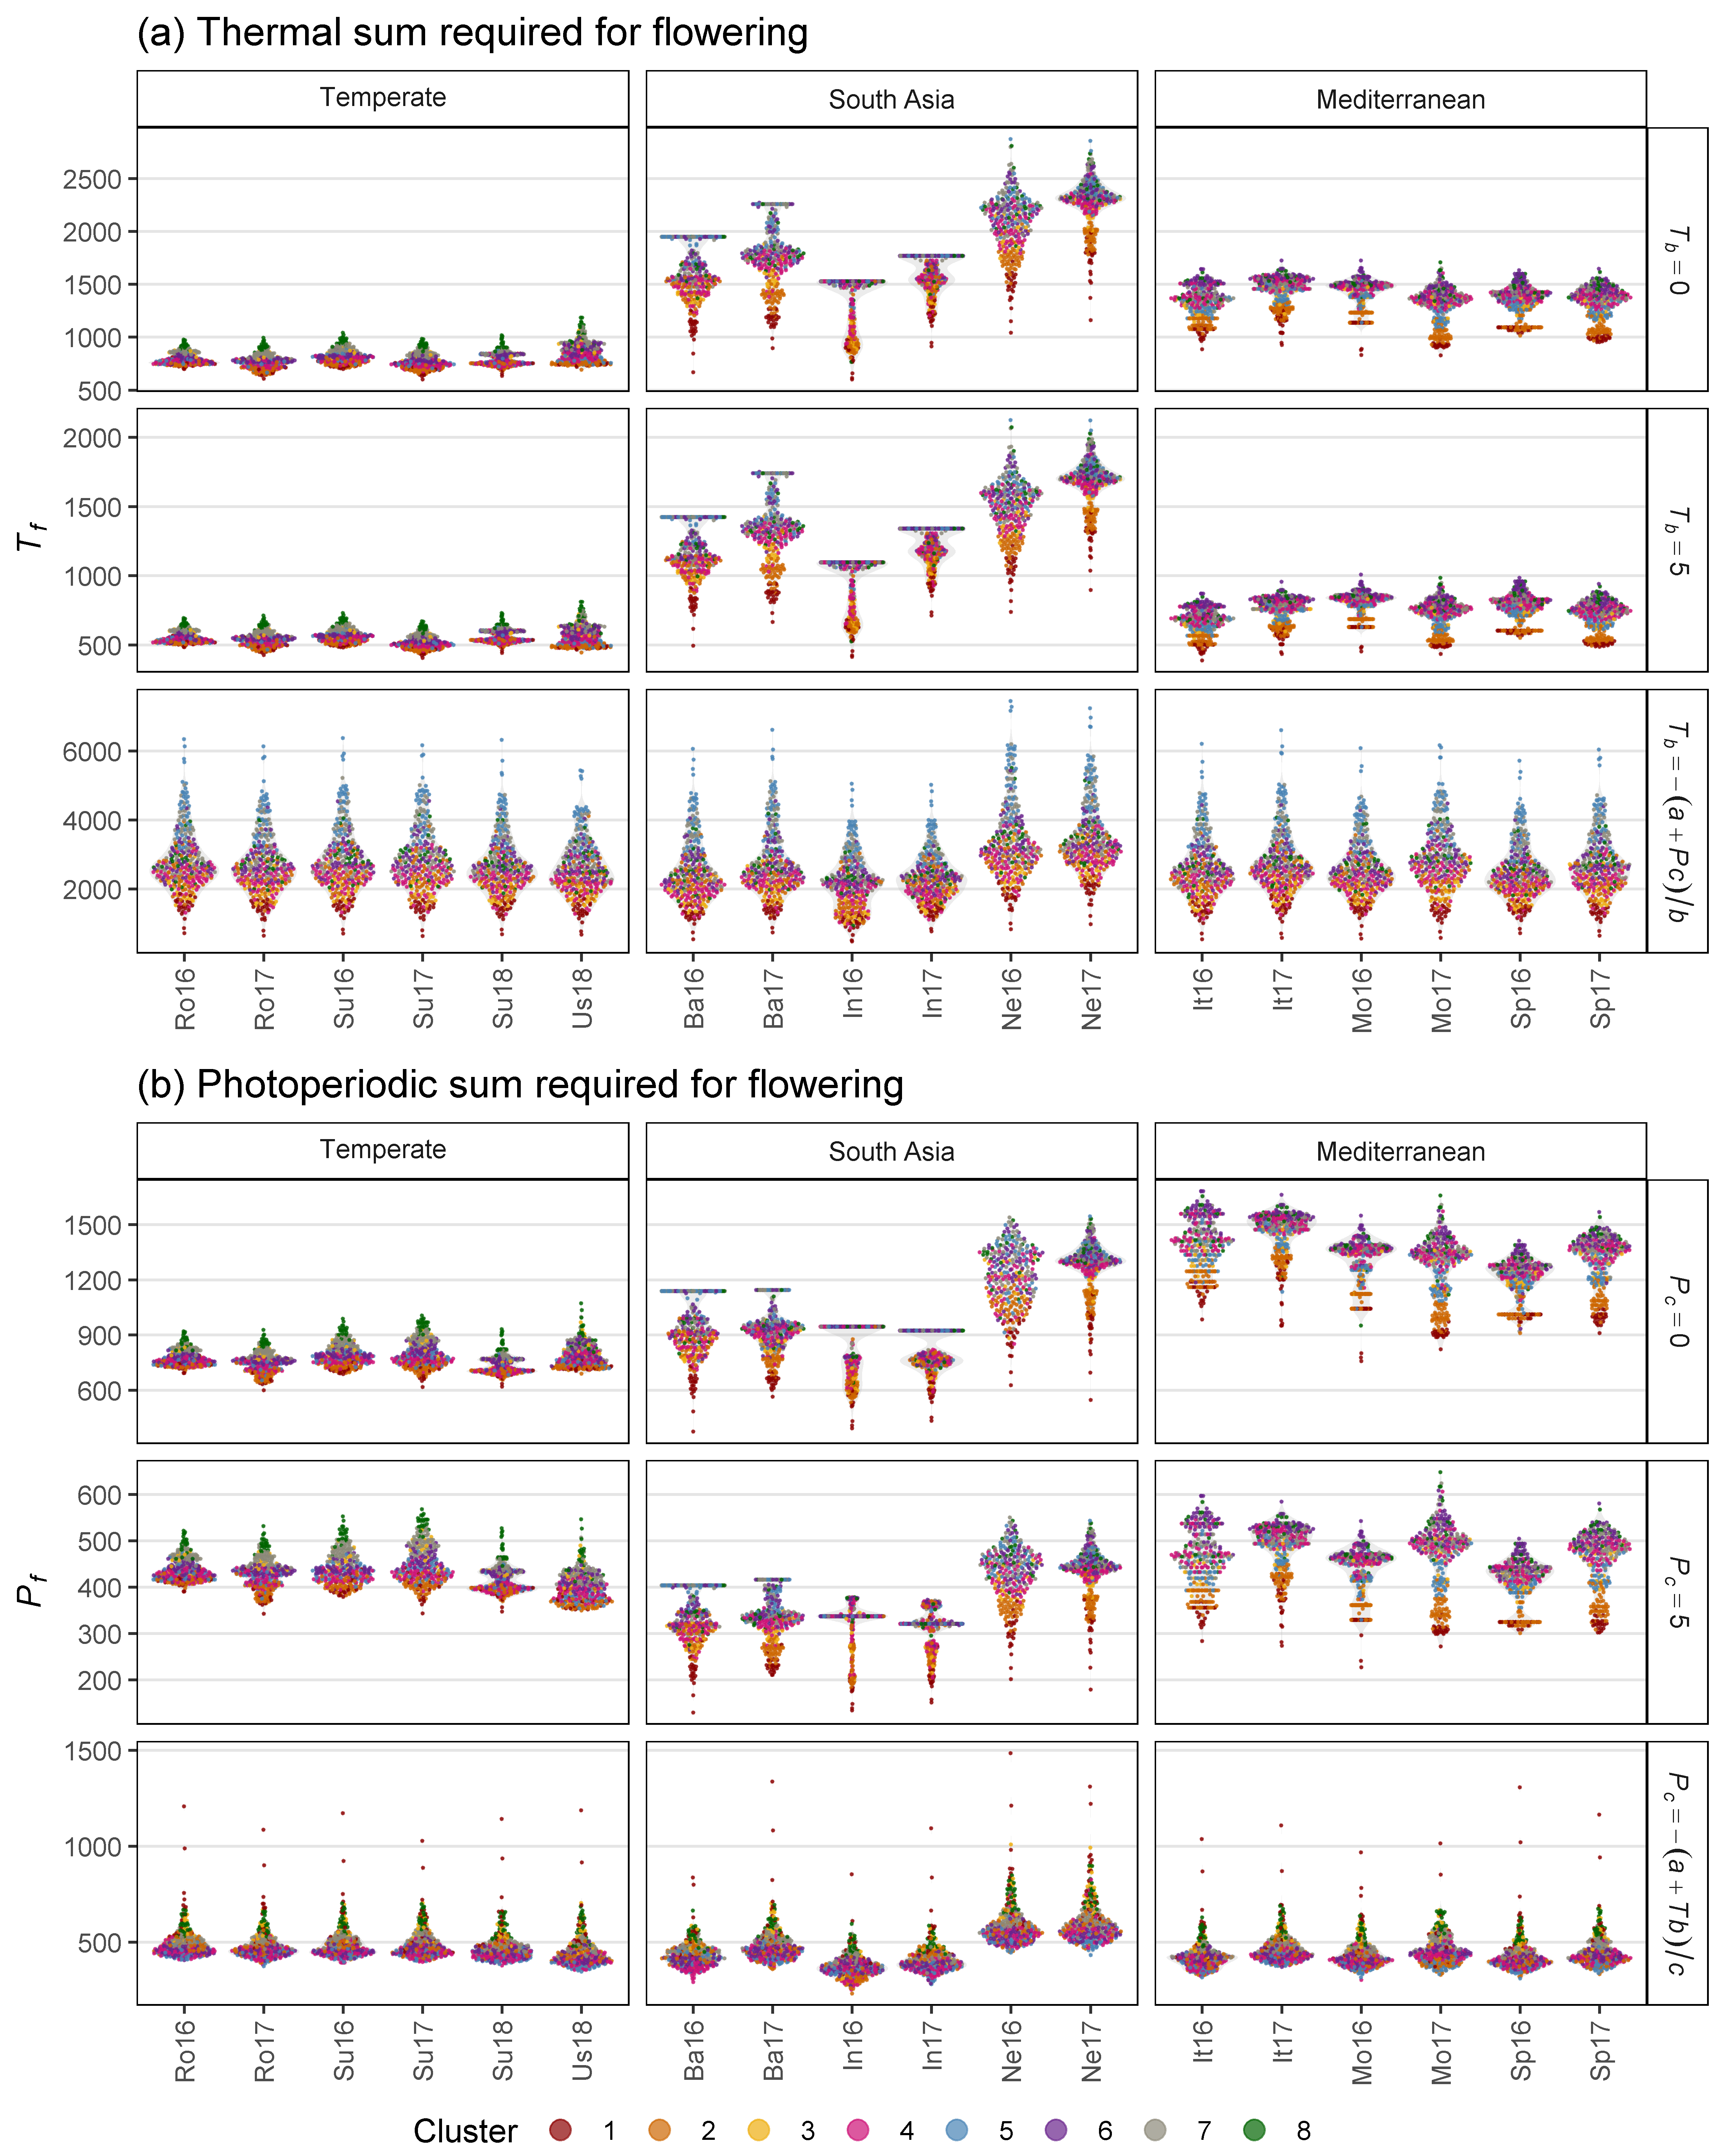
\includegraphics{Supplemental_Figure_09.png}

\begin{Shaded}
\begin{Highlighting}[]
\CommentTok{# Prep data for (a) Tf}
\NormalTok{pca <-}\StringTok{ }\KeywordTok{read.csv}\NormalTok{(}\StringTok{"data/data_pca_results.csv"}\NormalTok{) }\OperatorTok\StringTok{ }\KeywordTok{select}\NormalTok{(Entry, Cluster) }\OperatorTok
\StringTok{  }\KeywordTok{mutate}\NormalTok{(}\DataTypeTok{Cluster =} \KeywordTok{factor}\NormalTok{(Cluster))}
\NormalTok{xx <-}\StringTok{ }\KeywordTok{read.csv}\NormalTok{(}\StringTok{"data/data_tb_pc.csv"}\NormalTok{) }\OperatorTok\StringTok{ }
\StringTok{  }\KeywordTok{left_join}\NormalTok{(pca, }\DataTypeTok{by =} \StringTok{"Entry"}\NormalTok{) }\OperatorTok
\StringTok{  }\KeywordTok{mutate}\NormalTok{(}\DataTypeTok{MacroEnv =} \KeywordTok{factor}\NormalTok{(MacroEnv, }\DataTypeTok{levels =}\NormalTok{ macroEnvs))}
\NormalTok{x1 <-}\StringTok{ }\NormalTok{xx }\OperatorTok\StringTok{ }
\StringTok{  }\KeywordTok{select}\NormalTok{(Entry, Name, Expt, ExptShort, MacroEnv, Cluster, Tf_}\DecValTok{0}\NormalTok{, Tf_}\DecValTok{5}\NormalTok{, Tf) }\OperatorTok
\StringTok{  }\KeywordTok{gather}\NormalTok{(Trait, Value, Tf_}\DecValTok{0}\NormalTok{, Tf_}\DecValTok{5}\NormalTok{, Tf) }\OperatorTok
\StringTok{  }\KeywordTok{mutate}\NormalTok{(}\DataTypeTok{Trait =} \KeywordTok{factor}\NormalTok{(Trait, }\DataTypeTok{levels =} \KeywordTok{c}\NormalTok{(}\StringTok{"Tf_0"}\NormalTok{, }\StringTok{"Tf_5"}\NormalTok{, }\StringTok{"Tf"}\NormalTok{)))}
\NormalTok{new.lab <-}\StringTok{ }\KeywordTok{as_labeller}\NormalTok{(}\KeywordTok{c}\NormalTok{(}
  \DataTypeTok{Tf_0 =} \StringTok{"italic(T)[italic(b)]==0"}\NormalTok{, }\DataTypeTok{Tf_5 =} \StringTok{"italic(T)[italic(b)]==5"}\NormalTok{,}
  \DataTypeTok{Tf =} \StringTok{"italic(T)[italic(b)]==-(italic(a)+italic(Pc))/italic(b)"}\NormalTok{, }
  \DataTypeTok{Mediterranean =} \StringTok{"Mediterranean"}\NormalTok{, }\DataTypeTok{Temperate =} \StringTok{"Temperate"}\NormalTok{, }
  \StringTok{`}\DataTypeTok{South Asia}\StringTok{`}\NormalTok{ =}\StringTok{ "South~Asia"}\NormalTok{), label_parsed)}
\CommentTok{# Plot (a) Tf}
\NormalTok{mp1 <-}\StringTok{ }\KeywordTok{ggplot}\NormalTok{(x1, }\KeywordTok{aes}\NormalTok{(}\DataTypeTok{x =}\NormalTok{ ExptShort, }\DataTypeTok{y =}\NormalTok{ Value)) }\OperatorTok{+}
\StringTok{  }\KeywordTok{geom_violin}\NormalTok{(}\DataTypeTok{fill =} \StringTok{"grey"}\NormalTok{, }\DataTypeTok{alpha =} \FloatTok{0.3}\NormalTok{, }\DataTypeTok{color =} \OtherTok{NA}\NormalTok{) }\OperatorTok{+}\StringTok{ }
\StringTok{  }\KeywordTok{geom_quasirandom}\NormalTok{(}\KeywordTok{aes}\NormalTok{(}\DataTypeTok{color =}\NormalTok{ Cluster), }\DataTypeTok{size =} \FloatTok{0.1}\NormalTok{, }\DataTypeTok{alpha =} \FloatTok{0.7}\NormalTok{) }\OperatorTok{+}\StringTok{ }
\StringTok{  }\KeywordTok{facet_grid}\NormalTok{(Trait }\OperatorTok{~}\StringTok{ }\NormalTok{MacroEnv, }\DataTypeTok{scales =} \StringTok{"free"}\NormalTok{, }\DataTypeTok{labeller =}\NormalTok{ new.lab) }\OperatorTok{+}
\StringTok{  }\KeywordTok{scale_color_manual}\NormalTok{(}\DataTypeTok{values =}\NormalTok{ colors) }\OperatorTok{+}
\StringTok{  }\NormalTok{theme_AGL }\OperatorTok{+}
\StringTok{  }\KeywordTok{theme}\NormalTok{(}\DataTypeTok{legend.position =} \StringTok{"bottom"}\NormalTok{, }
        \DataTypeTok{legend.margin =} \KeywordTok{unit}\NormalTok{(}\KeywordTok{c}\NormalTok{(}\DecValTok{0}\NormalTok{,}\DecValTok{0}\NormalTok{,}\DecValTok{0}\NormalTok{,}\DecValTok{0}\NormalTok{), }\StringTok{"cm"}\NormalTok{),}
        \DataTypeTok{panel.grid.major.x =} \KeywordTok{element_blank}\NormalTok{(),}
        \DataTypeTok{axis.text.x =} \KeywordTok{element_text}\NormalTok{(}\DataTypeTok{angle =} \DecValTok{90}\NormalTok{, }\DataTypeTok{hjust =} \DecValTok{1}\NormalTok{, }\DataTypeTok{vjust =} \FloatTok{0.5}\NormalTok{)) }\OperatorTok{+}
\StringTok{  }\KeywordTok{guides}\NormalTok{(}\DataTypeTok{colour =} \KeywordTok{guide_legend}\NormalTok{(}\DataTypeTok{nrow =} \DecValTok{1}\NormalTok{, }\DataTypeTok{override.aes =} \KeywordTok{list}\NormalTok{(}\DataTypeTok{size =} \DecValTok{3}\NormalTok{))) }\OperatorTok{+}
\StringTok{  }\KeywordTok{labs}\NormalTok{(}\DataTypeTok{title =} \StringTok{"(a) Thermal sum required for flowering"}\NormalTok{, }
       \DataTypeTok{y =} \KeywordTok{expression}\NormalTok{(}\KeywordTok{italic}\NormalTok{(}\StringTok{"T"}\NormalTok{)[}\KeywordTok{italic}\NormalTok{(}\StringTok{"f"}\NormalTok{)]), }\DataTypeTok{x =} \OtherTok{NULL}\NormalTok{)}
\CommentTok{# Prep data for B) Pf}
\NormalTok{x1 <-}\StringTok{ }\NormalTok{xx }\OperatorTok\StringTok{ }
\StringTok{  }\KeywordTok{select}\NormalTok{(Entry, Expt, ExptShort, MacroEnv, Cluster, Pf_}\DecValTok{0}\NormalTok{, Pf_}\DecValTok{7}\NormalTok{, Pf) }\OperatorTok
\StringTok{  }\KeywordTok{gather}\NormalTok{(Trait, Value, Pf_}\DecValTok{0}\NormalTok{, Pf_}\DecValTok{7}\NormalTok{, Pf) }\OperatorTok
\StringTok{  }\KeywordTok{mutate}\NormalTok{(}\DataTypeTok{Trait =} \KeywordTok{factor}\NormalTok{(Trait, }\DataTypeTok{levels =} \KeywordTok{c}\NormalTok{(}\StringTok{"Pf_0"}\NormalTok{, }\StringTok{"Pf_7"}\NormalTok{, }\StringTok{"Pf"}\NormalTok{)))}
\NormalTok{new.lab <-}\StringTok{ }\KeywordTok{as_labeller}\NormalTok{(}\KeywordTok{c}\NormalTok{(}
  \DataTypeTok{Pf_0 =} \StringTok{"italic(P)[italic(c)]==0"}\NormalTok{, }\DataTypeTok{Pf_7 =} \StringTok{"italic(P)[italic(c)]==5"}\NormalTok{,}
  \DataTypeTok{Pf =} \StringTok{"italic(P)[italic(c)]==-(italic(a)+italic(Tb))/italic(c)"}\NormalTok{,}
  \DataTypeTok{Mediterranean =} \StringTok{"Mediterranean"}\NormalTok{, }\DataTypeTok{Temperate =} \StringTok{"Temperate"}\NormalTok{, }
  \StringTok{`}\DataTypeTok{South Asia}\StringTok{`}\NormalTok{ =}\StringTok{ "South~Asia"}\NormalTok{), label_parsed)}
\CommentTok{# Plot (b) Pf}
\NormalTok{mp2 <-}\StringTok{ }\KeywordTok{ggplot}\NormalTok{(x1, }\KeywordTok{aes}\NormalTok{(}\DataTypeTok{x =}\NormalTok{ ExptShort, }\DataTypeTok{y =}\NormalTok{ Value)) }\OperatorTok{+}
\StringTok{  }\KeywordTok{geom_violin}\NormalTok{(}\DataTypeTok{fill =} \StringTok{"grey"}\NormalTok{, }\DataTypeTok{alpha =} \FloatTok{0.3}\NormalTok{, }\DataTypeTok{color =} \OtherTok{NA}\NormalTok{) }\OperatorTok{+}\StringTok{ }
\StringTok{  }\KeywordTok{geom_quasirandom}\NormalTok{( }\KeywordTok{aes}\NormalTok{(}\DataTypeTok{color =}\NormalTok{ Cluster), }\DataTypeTok{size =} \FloatTok{0.1}\NormalTok{, }\DataTypeTok{alpha =} \FloatTok{0.7}\NormalTok{) }\OperatorTok{+}\StringTok{ }
\StringTok{  }\KeywordTok{facet_grid}\NormalTok{(Trait }\OperatorTok{~}\StringTok{ }\NormalTok{MacroEnv, }\DataTypeTok{scales =} \StringTok{"free"}\NormalTok{, }\DataTypeTok{labeller =}\NormalTok{ new.lab) }\OperatorTok{+}
\StringTok{  }\KeywordTok{scale_color_manual}\NormalTok{(}\DataTypeTok{values =}\NormalTok{ colors) }\OperatorTok{+}
\StringTok{  }\NormalTok{theme_AGL }\OperatorTok{+}
\StringTok{  }\KeywordTok{theme}\NormalTok{(}\DataTypeTok{legend.position =} \StringTok{"bottom"}\NormalTok{,}
        \DataTypeTok{panel.grid.major.x =} \KeywordTok{element_blank}\NormalTok{(),}
        \DataTypeTok{axis.text.x =} \KeywordTok{element_text}\NormalTok{(}\DataTypeTok{angle =} \DecValTok{90}\NormalTok{, }\DataTypeTok{hjust =} \DecValTok{1}\NormalTok{, }\DataTypeTok{vjust =} \FloatTok{0.5}\NormalTok{)) }\OperatorTok{+}
\StringTok{  }\KeywordTok{guides}\NormalTok{(}\DataTypeTok{colour =} \KeywordTok{guide_legend}\NormalTok{(}\DataTypeTok{nrow =} \DecValTok{1}\NormalTok{, }\DataTypeTok{override.aes =} \KeywordTok{list}\NormalTok{(}\DataTypeTok{size =} \DecValTok{3}\NormalTok{))) }\OperatorTok{+}
\StringTok{  }\KeywordTok{labs}\NormalTok{(}\DataTypeTok{title =} \StringTok{"(b) Photoperiodic sum required for flowering"}\NormalTok{, }
       \DataTypeTok{y =} \KeywordTok{expression}\NormalTok{(}\KeywordTok{italic}\NormalTok{(}\StringTok{"P"}\NormalTok{)[}\KeywordTok{italic}\NormalTok{(}\StringTok{"f"}\NormalTok{)]), }\DataTypeTok{x =} \OtherTok{NULL}\NormalTok{)}

\CommentTok{# Append (a), (b) and (c)}
\NormalTok{mp <-}\StringTok{ }\KeywordTok{ggarrange}\NormalTok{(mp1, mp2, }\DataTypeTok{ncol =} \DecValTok{1}\NormalTok{, }\DataTypeTok{common.legend =}\NormalTok{ T, }\DataTypeTok{legend =} \StringTok{"bottom"}\NormalTok{)}
\CommentTok{# Save}
\KeywordTok{ggsave}\NormalTok{(}\StringTok{"Additional/Temp/Temp_SF09_1.png"}\NormalTok{, mp1, }
       \DataTypeTok{width =} \DecValTok{10}\NormalTok{, }\DataTypeTok{height =} \DecValTok{13} \OperatorTok{*}\StringTok{ }\DecValTok{3} \OperatorTok{/}\StringTok{ }\FloatTok{8.2}\NormalTok{, }\DataTypeTok{dpi =} \DecValTok{600}\NormalTok{)}
\KeywordTok{ggsave}\NormalTok{(}\StringTok{"Additional/Temp/Temp_SF09_2.png"}\NormalTok{, mp2, }
       \DataTypeTok{width =} \DecValTok{10}\NormalTok{, }\DataTypeTok{height =} \DecValTok{13} \OperatorTok{*}\StringTok{ }\DecValTok{3} \OperatorTok{/}\StringTok{ }\FloatTok{8.2}\NormalTok{, }\DataTypeTok{dpi =} \DecValTok{600}\NormalTok{)}
\KeywordTok{ggsave}\NormalTok{(}\StringTok{"Supplemental_Figure_09.png"}\NormalTok{, mp, }\DataTypeTok{width =} \DecValTok{8}\NormalTok{, }\DataTypeTok{height =} \DecValTok{10}\NormalTok{, }\DataTypeTok{dpi =} \DecValTok{600}\NormalTok{)}
\end{Highlighting}
\end{Shaded}

\hypertarget{additional-figure-14-ptt}{%
\subsection{Additional Figure 14 PTT}\label{additional-figure-14-ptt}}

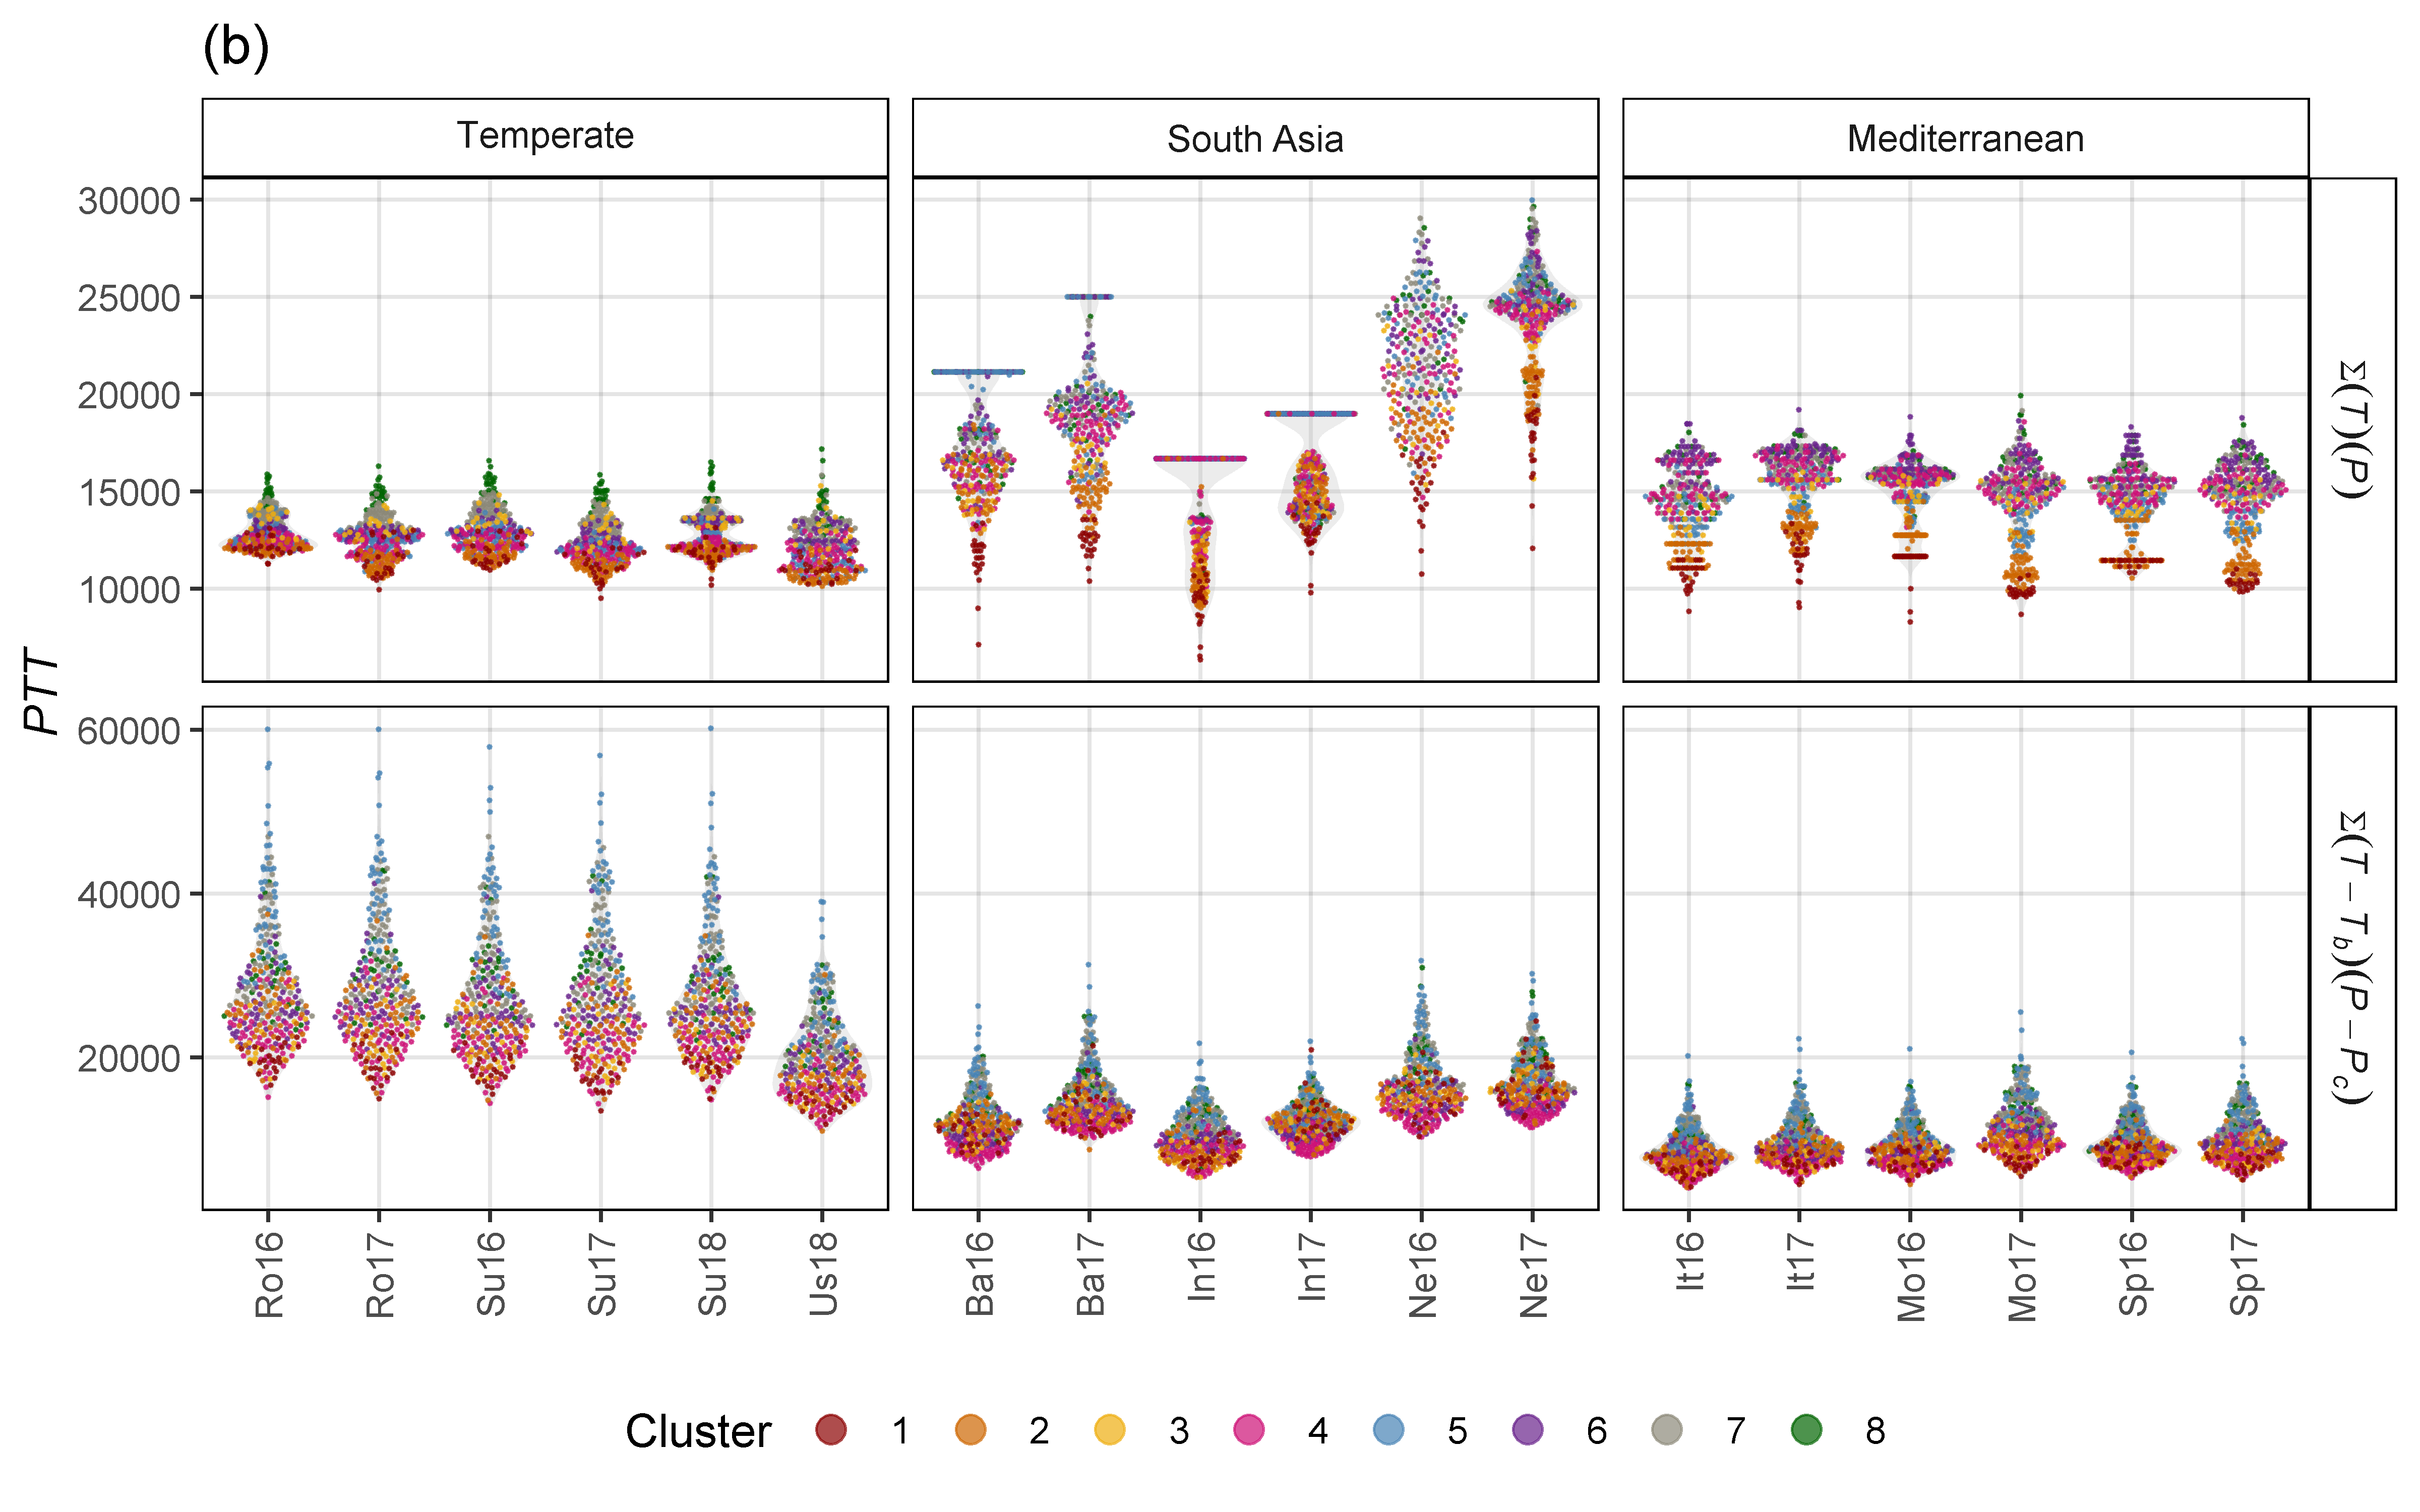
\includegraphics{Additional/Additional_Figure_14.png}

\begin{Shaded}
\begin{Highlighting}[]
\CommentTok{# Prep data}
\NormalTok{pca <-}\StringTok{ }\KeywordTok{read.csv}\NormalTok{(}\StringTok{"data/data_pca_results.csv"}\NormalTok{) }\OperatorTok\StringTok{ }\KeywordTok{select}\NormalTok{(Entry, Cluster) }\OperatorTok
\StringTok{  }\KeywordTok{mutate}\NormalTok{(}\DataTypeTok{Cluster =} \KeywordTok{factor}\NormalTok{(Cluster))}
\NormalTok{xx <-}\StringTok{ }\KeywordTok{read.csv}\NormalTok{(}\StringTok{"data/data_tb_pc.csv"}\NormalTok{) }\OperatorTok\StringTok{ }
\StringTok{  }\KeywordTok{left_join}\NormalTok{(pca, }\DataTypeTok{by =} \StringTok{"Entry"}\NormalTok{) }\OperatorTok
\StringTok{  }\KeywordTok{mutate}\NormalTok{(}\DataTypeTok{MacroEnv =} \KeywordTok{factor}\NormalTok{(MacroEnv, }\DataTypeTok{levels =}\NormalTok{ macroEnvs)) }\OperatorTok\StringTok{ }
\StringTok{  }\KeywordTok{select}\NormalTok{(Entry, Expt, ExptShort, MacroEnv, Cluster, PTT_}\DecValTok{0}\NormalTok{, PTT) }\OperatorTok
\StringTok{  }\KeywordTok{gather}\NormalTok{(Trait, Value, PTT_}\DecValTok{0}\NormalTok{, PTT) }\OperatorTok
\StringTok{  }\KeywordTok{mutate}\NormalTok{(}\DataTypeTok{Trait =} \KeywordTok{factor}\NormalTok{(Trait, }\DataTypeTok{levels =} \KeywordTok{c}\NormalTok{(}\StringTok{"PTT_0"}\NormalTok{, }\StringTok{"PTT"}\NormalTok{)))}
\NormalTok{new.lab <-}\StringTok{ }\KeywordTok{as_labeller}\NormalTok{(}\KeywordTok{c}\NormalTok{(}\DataTypeTok{PTT_0 =} \StringTok{"Sigma(italic(T))(italic(P))"}\NormalTok{,}
  \DataTypeTok{PTT =} \StringTok{"Sigma(italic(T)-italic(T)[italic(b)])(italic(P)-italic(P)[italic(c)])"}\NormalTok{, }
  \DataTypeTok{Mediterranean =} \StringTok{"Mediterranean"}\NormalTok{, }\DataTypeTok{Temperate =} \StringTok{"Temperate"}\NormalTok{, }
  \StringTok{`}\DataTypeTok{South Asia}\StringTok{`}\NormalTok{ =}\StringTok{ "South~Asia"}\NormalTok{), label_parsed)}
\CommentTok{# Plot PTT}
\NormalTok{mp <-}\StringTok{ }\KeywordTok{ggplot}\NormalTok{(xx, }\KeywordTok{aes}\NormalTok{(}\DataTypeTok{x =}\NormalTok{ ExptShort, }\DataTypeTok{y =}\NormalTok{ Value)) }\OperatorTok{+}
\StringTok{  }\KeywordTok{geom_violin}\NormalTok{(}\DataTypeTok{fill =} \StringTok{"grey"}\NormalTok{, }\DataTypeTok{alpha =} \FloatTok{0.3}\NormalTok{, }\DataTypeTok{color =} \OtherTok{NA}\NormalTok{) }\OperatorTok{+}\StringTok{ }
\StringTok{  }\KeywordTok{geom_quasirandom}\NormalTok{(}\KeywordTok{aes}\NormalTok{(}\DataTypeTok{color =}\NormalTok{ Cluster), }\DataTypeTok{size =} \FloatTok{0.1}\NormalTok{, }\DataTypeTok{alpha =} \FloatTok{0.7}\NormalTok{) }\OperatorTok{+}\StringTok{ }
\StringTok{  }\KeywordTok{facet_grid}\NormalTok{(Trait }\OperatorTok{~}\StringTok{ }\NormalTok{MacroEnv, }\DataTypeTok{scales =} \StringTok{"free"}\NormalTok{, }\DataTypeTok{labeller =}\NormalTok{ new.lab) }\OperatorTok{+}
\StringTok{  }\KeywordTok{scale_color_manual}\NormalTok{(}\DataTypeTok{values =}\NormalTok{ colors) }\OperatorTok{+}
\StringTok{  }\NormalTok{theme_AGL }\OperatorTok{+}
\StringTok{  }\KeywordTok{theme}\NormalTok{(}\DataTypeTok{legend.position =} \StringTok{"bottom"}\NormalTok{,}
        \DataTypeTok{panel.grid.major.x =} \KeywordTok{element_blank}\NormalTok{(),}
        \DataTypeTok{axis.text.x =} \KeywordTok{element_text}\NormalTok{(}\DataTypeTok{angle =} \DecValTok{90}\NormalTok{, }\DataTypeTok{hjust =} \DecValTok{1}\NormalTok{, }\DataTypeTok{vjust =} \FloatTok{0.5}\NormalTok{)) }\OperatorTok{+}
\StringTok{  }\KeywordTok{guides}\NormalTok{(}\DataTypeTok{colour =} \KeywordTok{guide_legend}\NormalTok{(}\DataTypeTok{nrow =} \DecValTok{1}\NormalTok{, }\DataTypeTok{override.aes =} \KeywordTok{list}\NormalTok{(}\DataTypeTok{size =} \DecValTok{3}\NormalTok{))) }\OperatorTok{+}
\StringTok{  }\KeywordTok{labs}\NormalTok{(}\DataTypeTok{title =} \StringTok{"(b)"}\NormalTok{, }\DataTypeTok{y =} \KeywordTok{expression}\NormalTok{(}\KeywordTok{italic}\NormalTok{(}\StringTok{"PTT"}\NormalTok{)), }\DataTypeTok{x =} \OtherTok{NULL}\NormalTok{)}
\KeywordTok{ggsave}\NormalTok{(}\StringTok{"Additional/Additional_Figure_14.png"}\NormalTok{, mp, }\DataTypeTok{width =} \DecValTok{8}\NormalTok{, }\DataTypeTok{height =} \DecValTok{5}\NormalTok{, }\DataTypeTok{dpi =} \DecValTok{600}\NormalTok{)}
\end{Highlighting}
\end{Shaded}

\hypertarget{supplemental-figure-10-thermal-sums}{%
\subsection{Supplemental Figure 10 Thermal
Sums}\label{supplemental-figure-10-thermal-sums}}

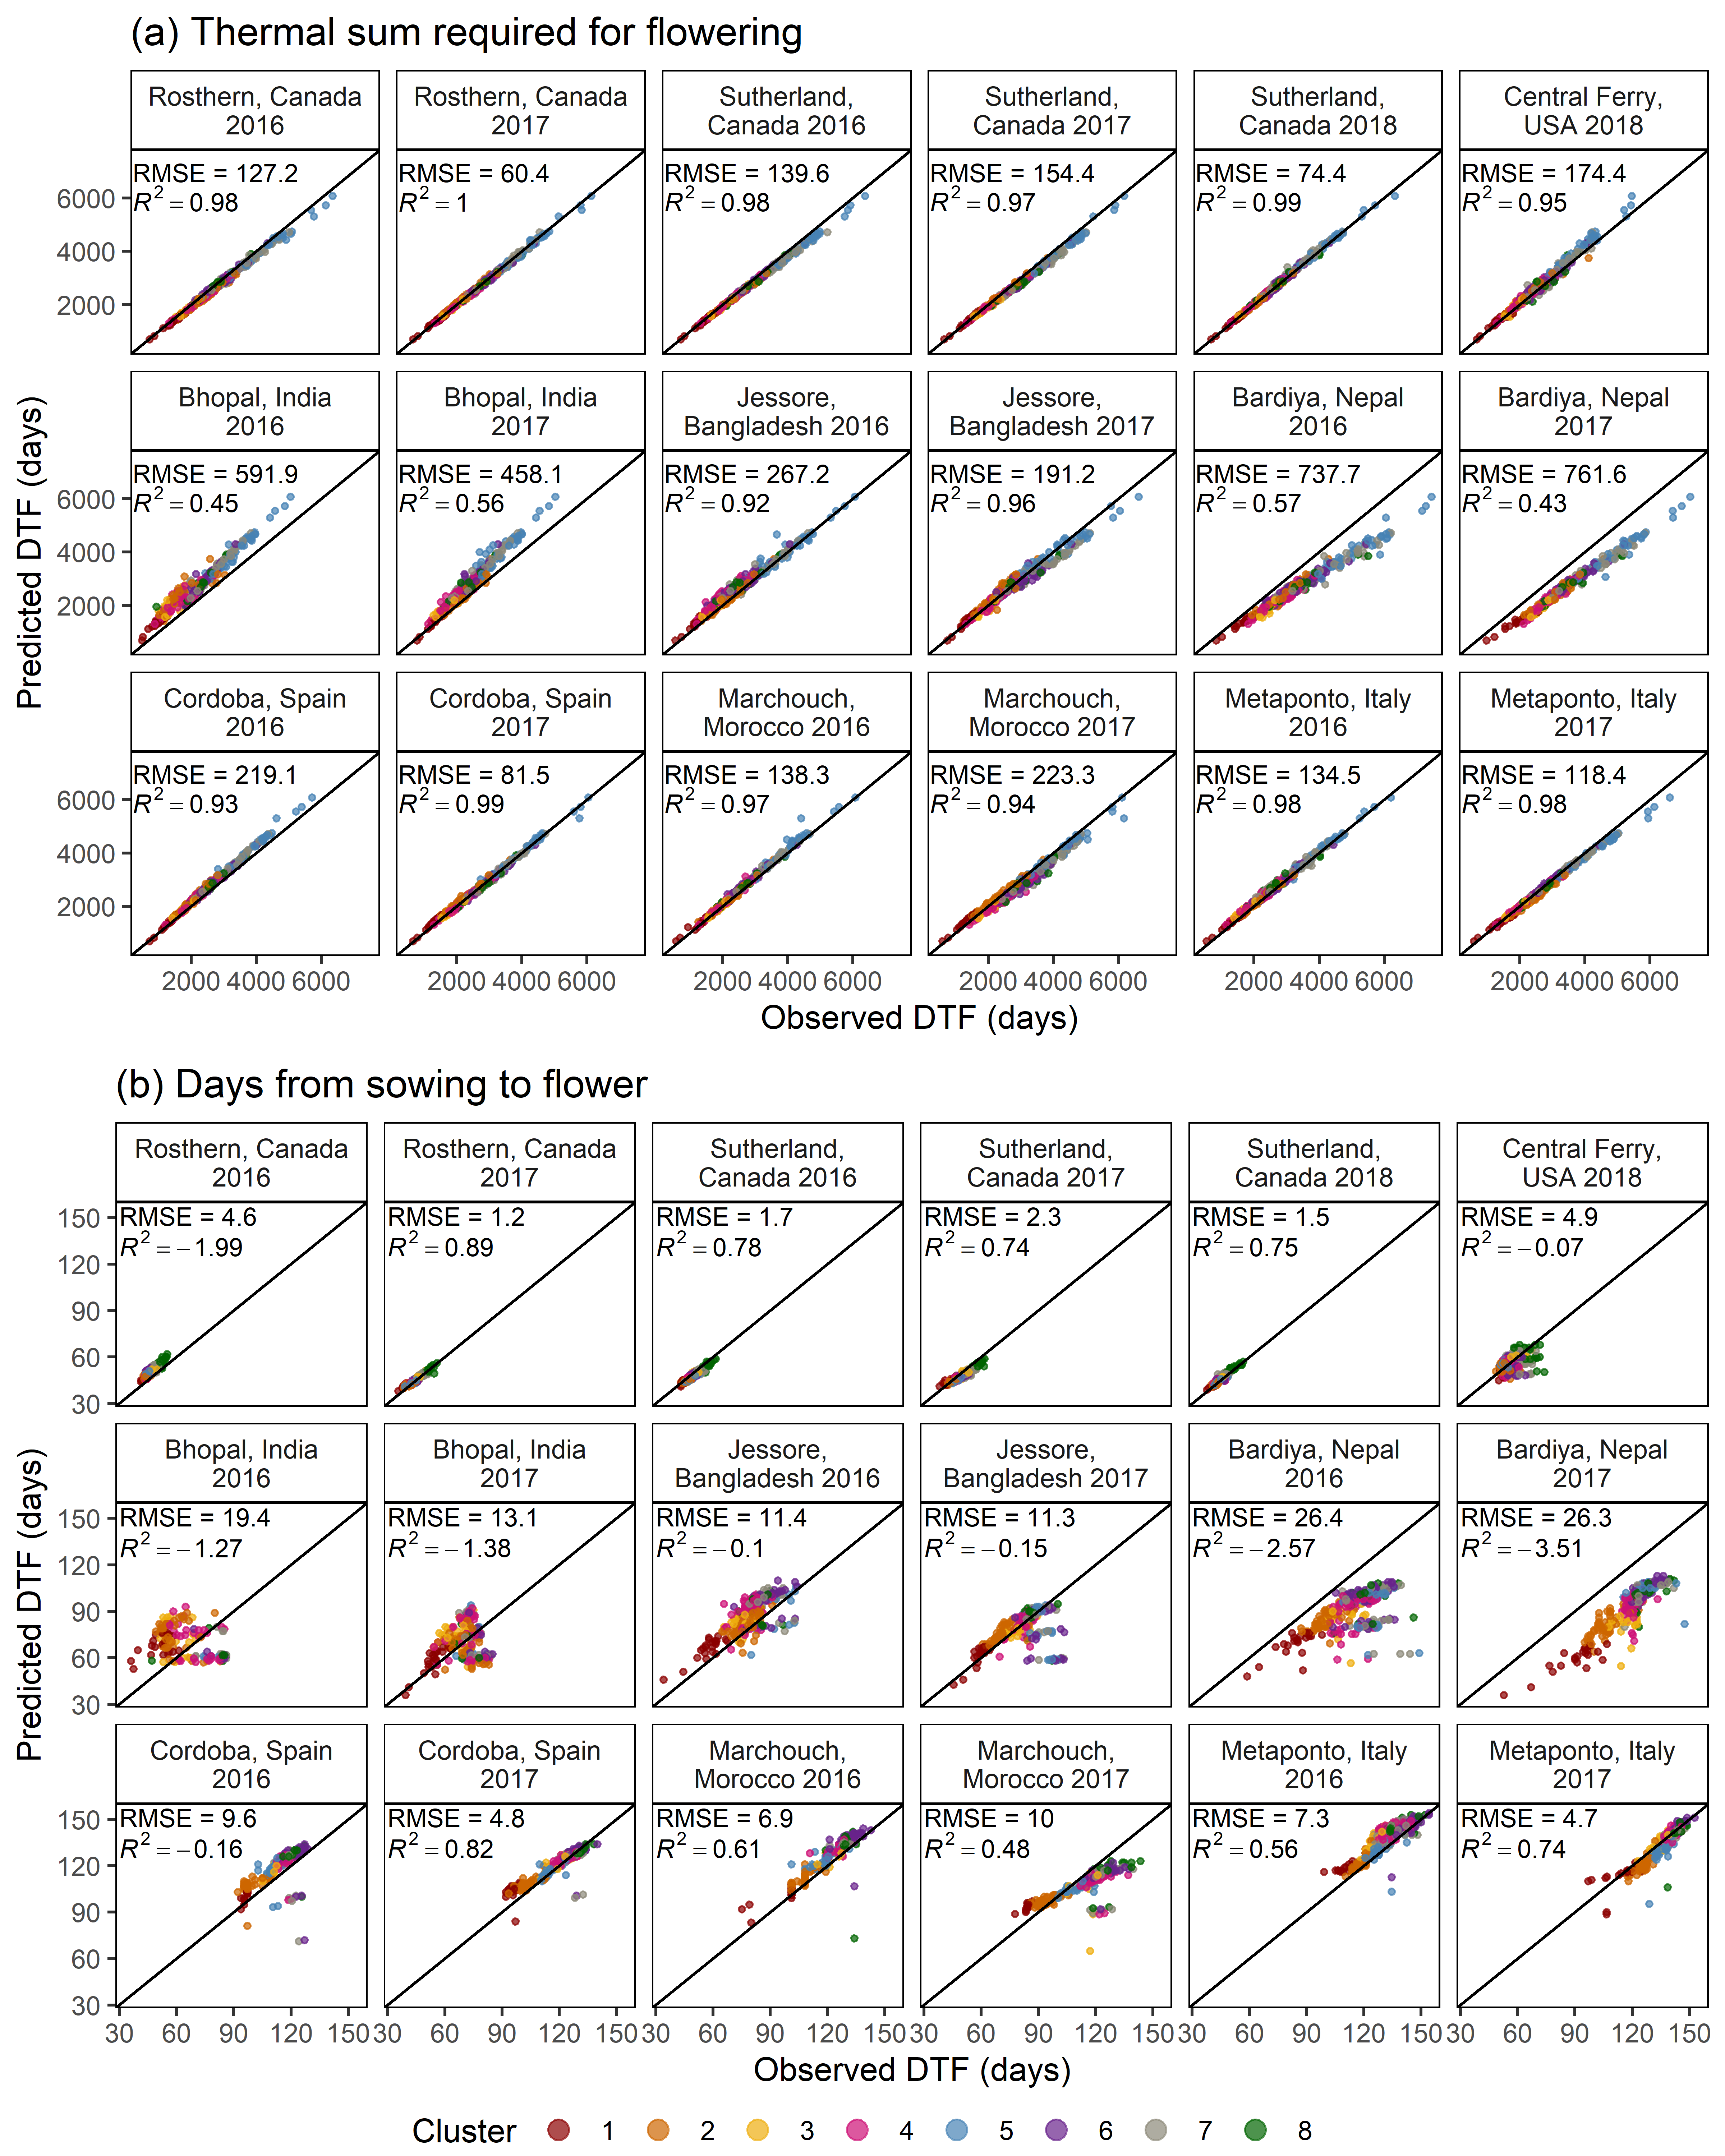
\includegraphics{Supplemental_Figure_10.png}

\begin{Shaded}
\begin{Highlighting}[]
\CommentTok{# Prep data}
\NormalTok{xx <-}\StringTok{ }\KeywordTok{read.csv}\NormalTok{(}\StringTok{"data/data_tb_pc.csv"}\NormalTok{) }\OperatorTok\StringTok{ }\CommentTok{#select(-MacroEnv) %>%}
\StringTok{  }\KeywordTok{mutate}\NormalTok{(}\DataTypeTok{Expt =} \KeywordTok{factor}\NormalTok{(Expt, }\DataTypeTok{levels =}\NormalTok{ names_Expt))}
\CommentTok{# Plot (a)}
\NormalTok{mp1 <-}\StringTok{ }\KeywordTok{gg_model_2}\NormalTok{(xx, }\StringTok{"Tf"}\NormalTok{, }\StringTok{"predicted_Tf"}\NormalTok{, }\StringTok{"(a) Thermal sum required for flowering"}\NormalTok{,}
                  \DecValTok{200}\NormalTok{, }\DecValTok{200}\NormalTok{, }\DecValTok{6600}\NormalTok{, }\DecValTok{5500}\NormalTok{)}
\CommentTok{# Plot (b)}
\NormalTok{mp2 <-}\StringTok{ }\KeywordTok{gg_model_2}\NormalTok{(xx, }\StringTok{"DTF"}\NormalTok{, }\StringTok{"predicted_DTF_Tf"}\NormalTok{, }\StringTok{"(b) Days from sowing to flower"}\NormalTok{,}
                  \DecValTok{30}\NormalTok{, }\DecValTok{30}\NormalTok{, }\DecValTok{145}\NormalTok{, }\DecValTok{125}\NormalTok{)}
\CommentTok{# Append (a) and (b)}
\NormalTok{mp <-}\StringTok{ }\KeywordTok{ggarrange}\NormalTok{(mp1, mp2, }\DataTypeTok{nrow =} \DecValTok{2}\NormalTok{, }\DataTypeTok{ncol =} \DecValTok{1}\NormalTok{, }\DataTypeTok{common.legend =}\NormalTok{ T, }\DataTypeTok{legend =} \StringTok{"bottom"}\NormalTok{)}
\KeywordTok{ggsave}\NormalTok{(}\StringTok{"Supplemental_Figure_10.png"}\NormalTok{, mp, }\DataTypeTok{width =} \DecValTok{8}\NormalTok{, }\DataTypeTok{height =} \DecValTok{10}\NormalTok{, }\DataTypeTok{dpi =} \DecValTok{600}\NormalTok{)}
\end{Highlighting}
\end{Shaded}

\hypertarget{supplemental-figure-11-photoperiodic-sums}{%
\subsection{Supplemental Figure 11 Photoperiodic
Sums}\label{supplemental-figure-11-photoperiodic-sums}}

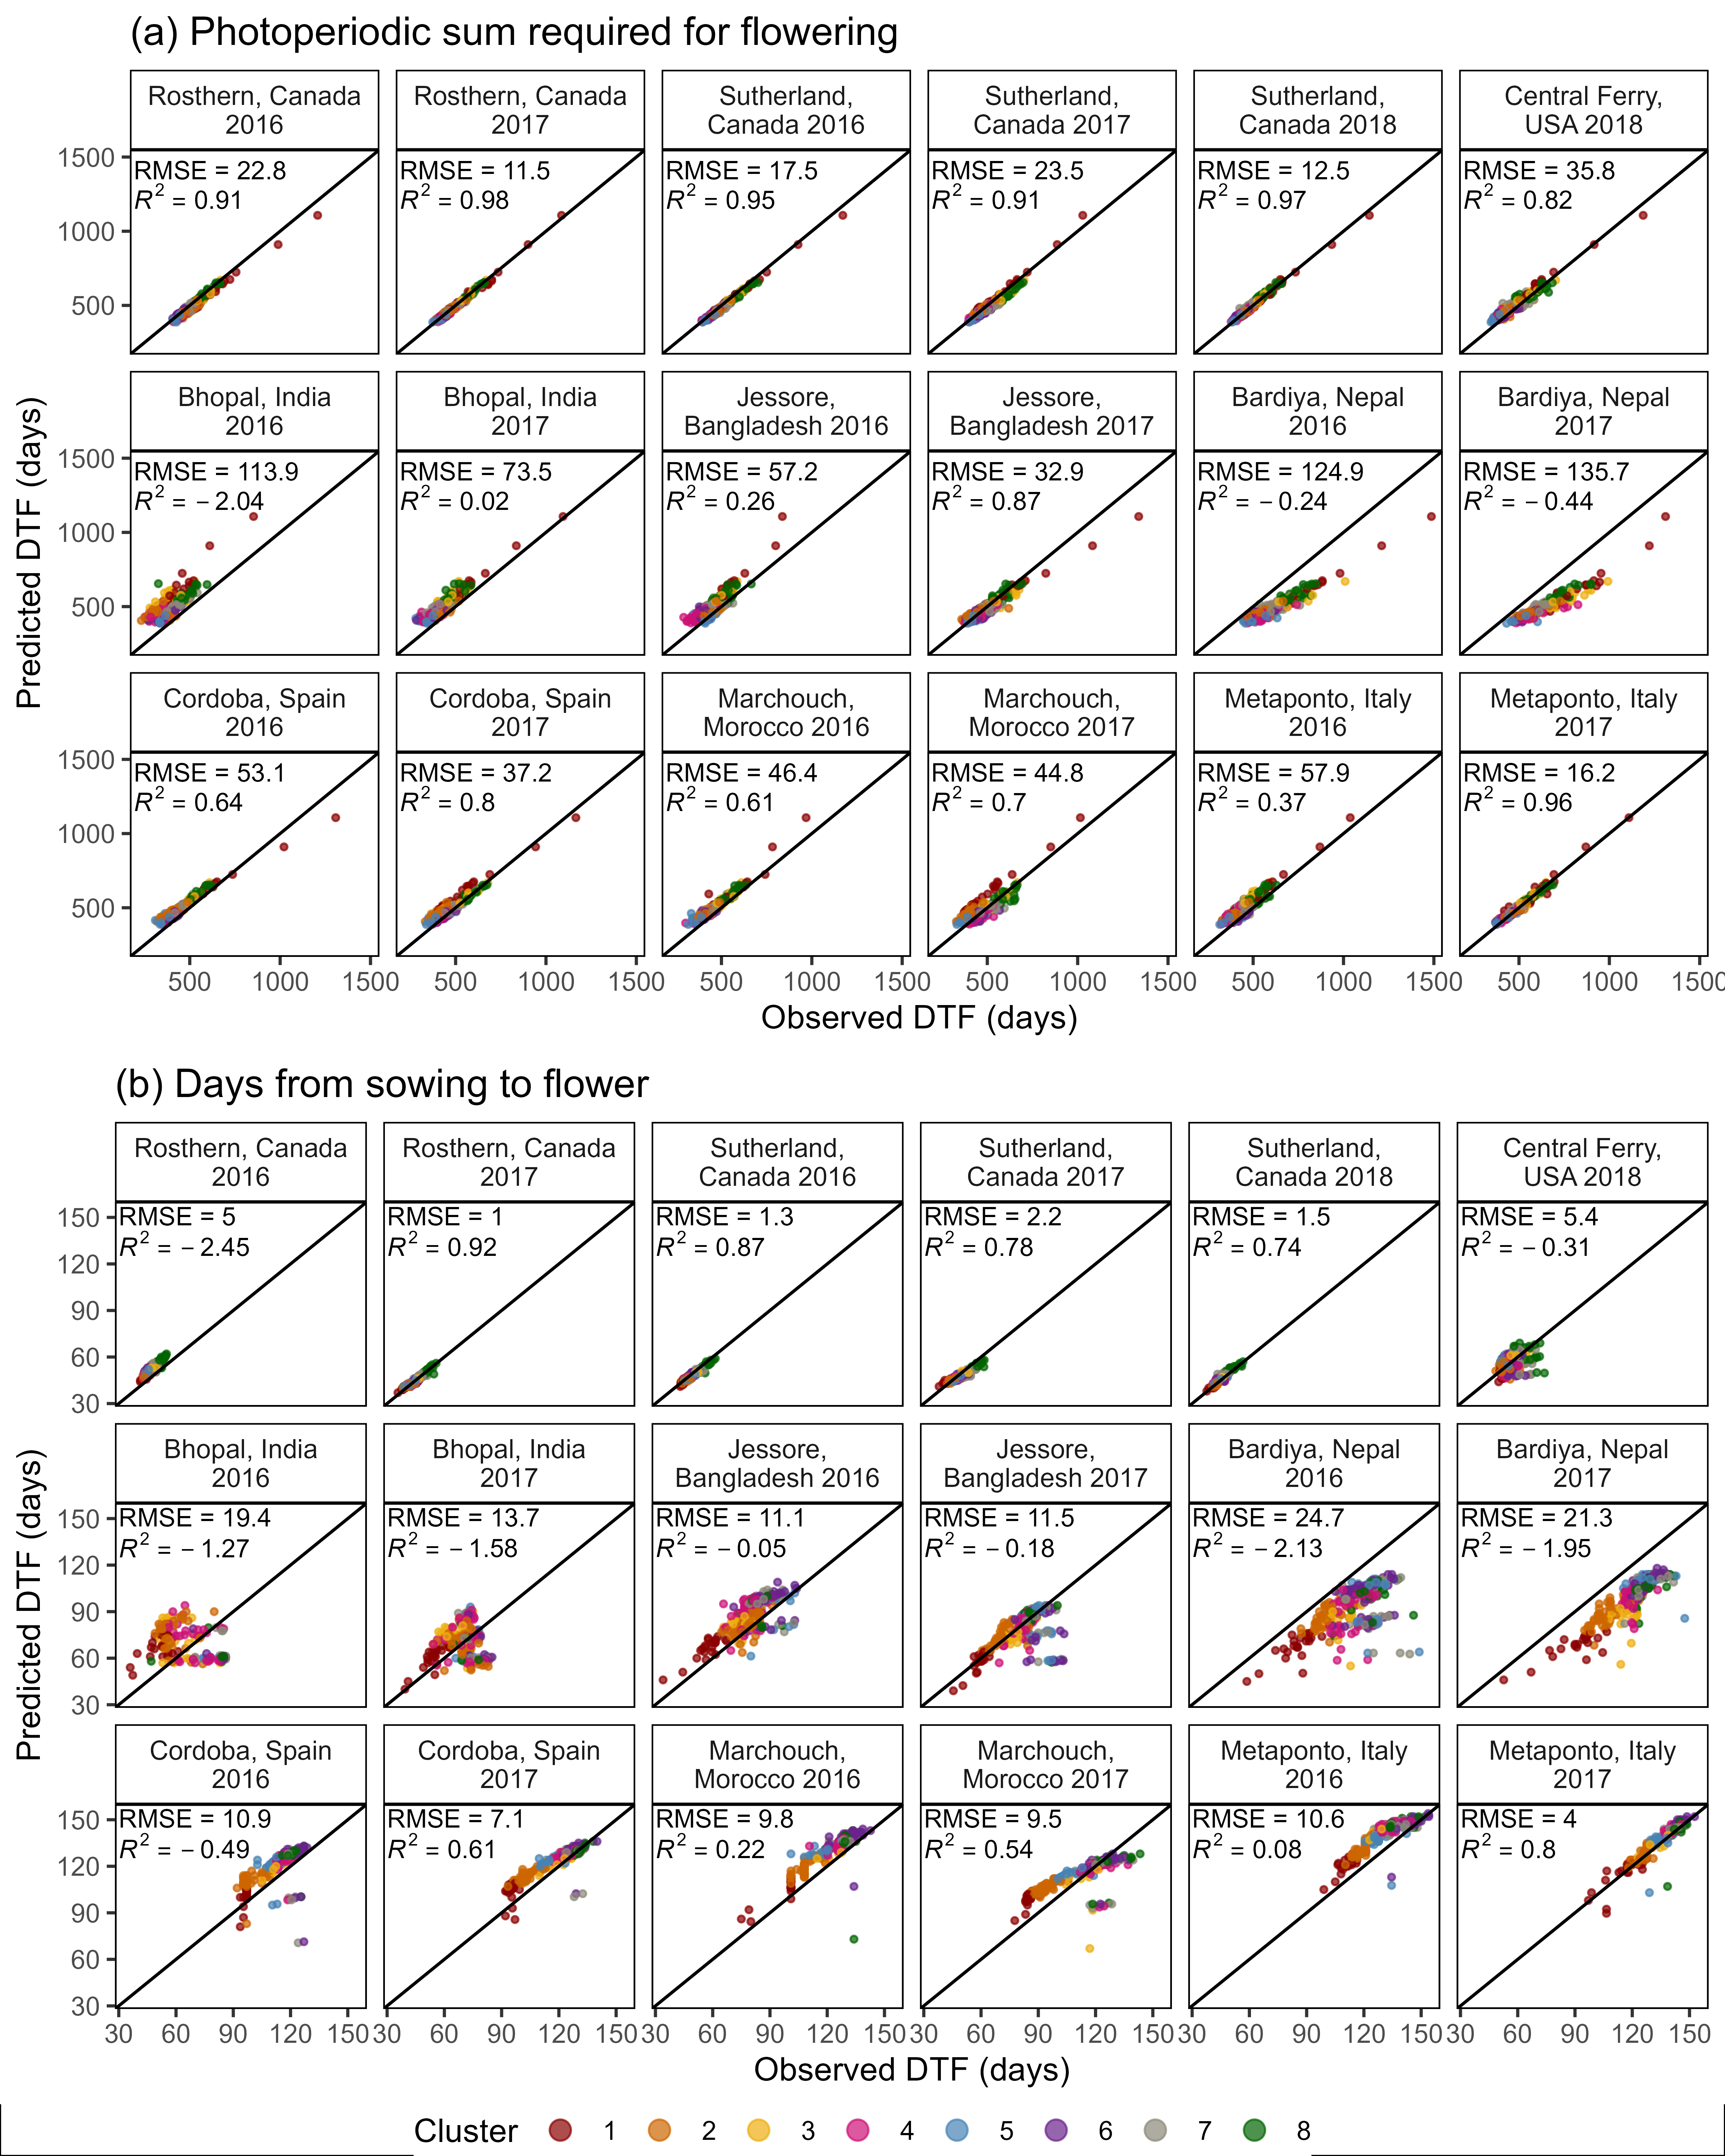
\includegraphics{Supplemental_Figure_11.png}

\begin{Shaded}
\begin{Highlighting}[]
\CommentTok{# Prep data}
\NormalTok{xx <-}\StringTok{ }\KeywordTok{read.csv}\NormalTok{(}\StringTok{"data/data_tb_pc.csv"}\NormalTok{) }\OperatorTok\StringTok{ }\CommentTok{#select(-MacroEnv) %>%}
\StringTok{  }\KeywordTok{mutate}\NormalTok{(}\DataTypeTok{Expt =} \KeywordTok{factor}\NormalTok{(Expt, }\DataTypeTok{levels =}\NormalTok{ names_Expt))}
\CommentTok{# Plot (a)}
\NormalTok{mp1 <-}\StringTok{ }\KeywordTok{gg_model_2}\NormalTok{(xx, }\StringTok{"Pf"}\NormalTok{, }\StringTok{"predicted_Pf"}\NormalTok{, }\StringTok{"(a) Photoperiodic sum required for flowering"}\NormalTok{,}
                  \DecValTok{190}\NormalTok{, }\DecValTok{190}\NormalTok{, }\DecValTok{1350}\NormalTok{, }\DecValTok{1150}\NormalTok{)}
\CommentTok{# Plot (b)}
\NormalTok{mp2 <-}\StringTok{ }\KeywordTok{gg_model_2}\NormalTok{(xx, }\StringTok{"DTF"}\NormalTok{, }\StringTok{"predicted_DTF_Pf"}\NormalTok{, }\StringTok{"(b) Days from sowing to flower"}\NormalTok{,}
                  \DecValTok{30}\NormalTok{, }\DecValTok{30}\NormalTok{, }\DecValTok{145}\NormalTok{, }\DecValTok{125}\NormalTok{)}
\CommentTok{# Append (a) and (b)}
\NormalTok{mp <-}\StringTok{ }\KeywordTok{ggarrange}\NormalTok{(mp1, mp2, }\DataTypeTok{nrow =} \DecValTok{2}\NormalTok{, }\DataTypeTok{ncol =} \DecValTok{1}\NormalTok{, }\DataTypeTok{common.legend =}\NormalTok{ T, }\DataTypeTok{legend =} \StringTok{"bottom"}\NormalTok{)}
\KeywordTok{ggsave}\NormalTok{(}\StringTok{"Supplemental_Figure_11.png"}\NormalTok{, mp, }\DataTypeTok{width =} \DecValTok{8}\NormalTok{, }\DataTypeTok{height =} \DecValTok{10}\NormalTok{, }\DataTypeTok{dpi =} \DecValTok{600}\NormalTok{)}
\end{Highlighting}
\end{Shaded}

\hypertarget{figure-7-temperature-increase-by-macroenv}{%
\subsection{Figure 7 Temperature Increase By
MacroEnv}\label{figure-7-temperature-increase-by-macroenv}}

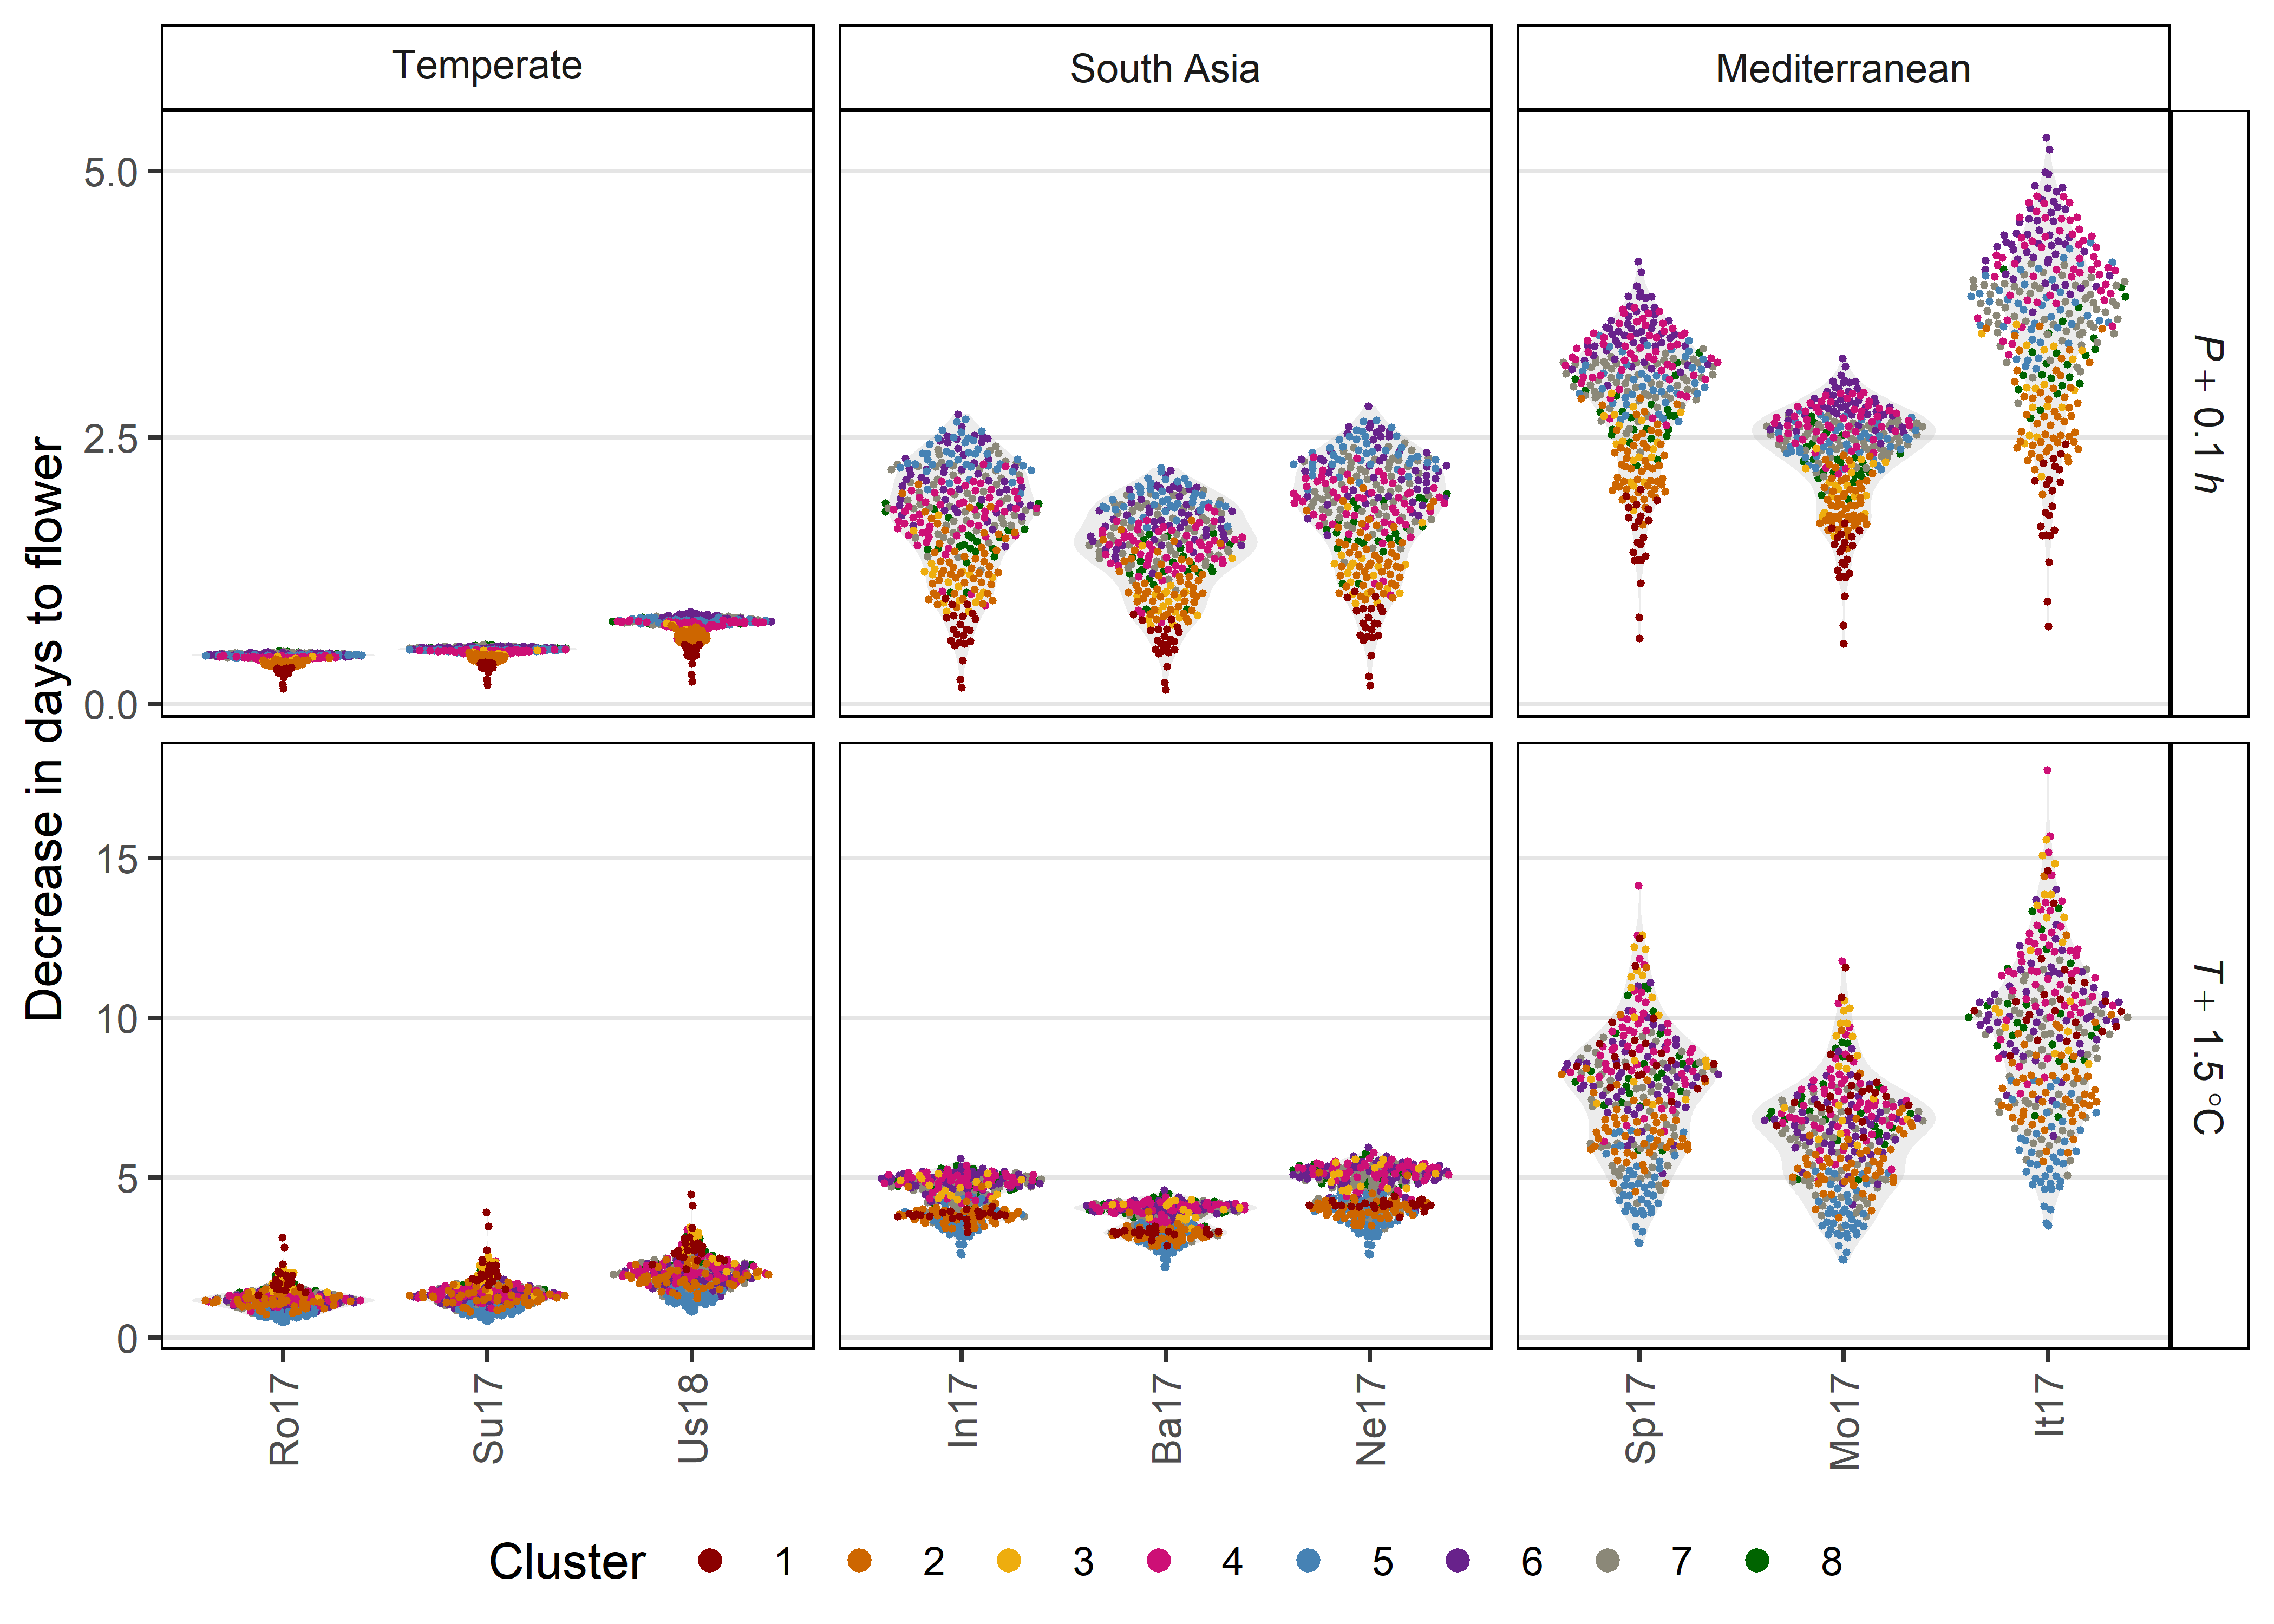
\includegraphics{Figure_07.png}

\begin{Shaded}
\begin{Highlighting}[]
\CommentTok{# Prep data}
\NormalTok{yy <-}\StringTok{ }\KeywordTok{c}\NormalTok{(}\StringTok{"Ro17"}\NormalTok{, }\StringTok{"Su17"}\NormalTok{, }\StringTok{"Us18"}\NormalTok{, }\StringTok{"In17"}\NormalTok{, }\StringTok{"Ba17"}\NormalTok{, }\StringTok{"Ne17"}\NormalTok{, }\StringTok{"Sp17"}\NormalTok{, }\StringTok{"Mo17"}\NormalTok{, }\StringTok{"It17"}\NormalTok{)}
\NormalTok{coefs <-}\StringTok{ }\KeywordTok{read.csv}\NormalTok{(}\StringTok{"data/model_t+p_coefs.csv"}\NormalTok{)}
\NormalTok{pca <-}\StringTok{ }\KeywordTok{read.csv}\NormalTok{(}\StringTok{"data/data_pca_results.csv"}\NormalTok{) }\OperatorTok\StringTok{ }\KeywordTok{select}\NormalTok{(Entry, Cluster) }\OperatorTok
\StringTok{  }\KeywordTok{mutate}\NormalTok{(}\DataTypeTok{Cluster =} \KeywordTok{factor}\NormalTok{(Cluster))}
\NormalTok{xx <-}\StringTok{ }\NormalTok{dd }\OperatorTok\StringTok{ }
\StringTok{  }\KeywordTok{select}\NormalTok{(Entry, Expt, ExptShort, DTF) }\OperatorTok\StringTok{ }
\StringTok{  }\KeywordTok{left_join}\NormalTok{(coefs, }\DataTypeTok{by =} \StringTok{"Entry"}\NormalTok{) }\OperatorTok
\StringTok{  }\KeywordTok{left_join}\NormalTok{(pca, }\DataTypeTok{by =} \StringTok{"Entry"}\NormalTok{) }\OperatorTok
\StringTok{  }\KeywordTok{left_join}\NormalTok{(}\KeywordTok{select}\NormalTok{(ff, Expt, MacroEnv, T_mean, P_mean), }\DataTypeTok{by =} \StringTok{"Expt"}\NormalTok{)}
\CommentTok{# Temp +1}
\NormalTok{x1 <-}\StringTok{ }\NormalTok{xx }\OperatorTok
\StringTok{  }\KeywordTok{mutate}\NormalTok{(}\DataTypeTok{T_mean_1.5 =}\NormalTok{ T_mean }\OperatorTok{+}\StringTok{ }\FloatTok{1.5}\NormalTok{,}
         \DataTypeTok{DTF_1 =} \DecValTok{1} \OperatorTok{/}\StringTok{ }\NormalTok{(a }\OperatorTok{+}\StringTok{ }\NormalTok{b }\OperatorTok{*}\StringTok{ }\NormalTok{T_mean_}\FloatTok{1.5} \OperatorTok{+}\StringTok{ }\NormalTok{c }\OperatorTok{*}\StringTok{ }\NormalTok{P_mean),}
         \DataTypeTok{DTF_0  =} \DecValTok{1} \OperatorTok{/}\StringTok{ }\NormalTok{(a }\OperatorTok{+}\StringTok{ }\NormalTok{b }\OperatorTok{*}\StringTok{ }\NormalTok{T_mean }\OperatorTok{+}\StringTok{ }\NormalTok{c }\OperatorTok{*}\StringTok{ }\NormalTok{P_mean),}
         \DataTypeTok{Difference =}\NormalTok{ DTF_}\DecValTok{0} \OperatorTok{-}\StringTok{ }\NormalTok{DTF_}\DecValTok{1}\NormalTok{) }\OperatorTok\StringTok{ }
\StringTok{  }\KeywordTok{filter}\NormalTok{(ExptShort }\OperatorTok\StringTok{ }\NormalTok{yy)}
\NormalTok{x2 <-}\StringTok{ }\NormalTok{xx }\OperatorTok
\StringTok{  }\KeywordTok{mutate}\NormalTok{(}\DataTypeTok{P_mean_0.1 =}\NormalTok{ P_mean }\OperatorTok{+}\StringTok{ }\FloatTok{0.1}\NormalTok{,}
         \DataTypeTok{DTF_1 =} \DecValTok{1} \OperatorTok{/}\StringTok{ }\NormalTok{(a }\OperatorTok{+}\StringTok{ }\NormalTok{b }\OperatorTok{*}\StringTok{ }\NormalTok{T_mean }\OperatorTok{+}\StringTok{ }\NormalTok{c }\OperatorTok{*}\StringTok{ }\NormalTok{P_mean_}\FloatTok{0.1}\NormalTok{),}
         \DataTypeTok{DTF_0  =} \DecValTok{1} \OperatorTok{/}\StringTok{ }\NormalTok{(a }\OperatorTok{+}\StringTok{ }\NormalTok{b }\OperatorTok{*}\StringTok{ }\NormalTok{T_mean }\OperatorTok{+}\StringTok{ }\NormalTok{c }\OperatorTok{*}\StringTok{ }\NormalTok{P_mean),}
         \DataTypeTok{Difference =}\NormalTok{ DTF_}\DecValTok{0} \OperatorTok{-}\StringTok{ }\NormalTok{DTF_}\DecValTok{1}\NormalTok{) }\OperatorTok\StringTok{ }
\StringTok{  }\KeywordTok{filter}\NormalTok{(ExptShort }\OperatorTok\StringTok{ }\NormalTok{yy)}
\NormalTok{x1 <-}\StringTok{ }\NormalTok{x1 }\OperatorTok\StringTok{ }\KeywordTok{mutate}\NormalTok{(}\DataTypeTok{Treatment =} \StringTok{"T + 1.5"}\NormalTok{)}
\NormalTok{x2 <-}\StringTok{ }\NormalTok{x2 }\OperatorTok\StringTok{ }\KeywordTok{mutate}\NormalTok{(}\DataTypeTok{Treatment =} \StringTok{"P + 0.1"}\NormalTok{)}
\NormalTok{knitr}\OperatorTok{::}\KeywordTok{kable}\NormalTok{(x1 }\OperatorTok\StringTok{ }\KeywordTok{group_by}\NormalTok{(MacroEnv) }\OperatorTok\StringTok{ }
\StringTok{  }\KeywordTok{summarise}\NormalTok{(}\DataTypeTok{Min =} \KeywordTok{round}\NormalTok{(}\KeywordTok{min}\NormalTok{(Difference), }\DecValTok{2}\NormalTok{), }\DataTypeTok{Max =} \KeywordTok{round}\NormalTok{(}\KeywordTok{max}\NormalTok{(Difference), }\DecValTok{2}\NormalTok{)) )}
\end{Highlighting}
\end{Shaded}

\begin{longtable}[]{@{}lrr@{}}
\toprule
MacroEnv & Min & Max\tabularnewline
\midrule
\endhead
Temperate & 0.48 & 4.48\tabularnewline
South Asia & 2.21 & 5.96\tabularnewline
Mediterranean & 2.43 & 17.76\tabularnewline
\bottomrule
\end{longtable}

\begin{Shaded}
\begin{Highlighting}[]
\NormalTok{knitr}\OperatorTok{::}\KeywordTok{kable}\NormalTok{(x2 }\OperatorTok\StringTok{ }\KeywordTok{group_by}\NormalTok{(MacroEnv) }\OperatorTok\StringTok{ }
\StringTok{  }\KeywordTok{summarise}\NormalTok{(}\DataTypeTok{Min =} \KeywordTok{round}\NormalTok{(}\KeywordTok{min}\NormalTok{(Difference), }\DecValTok{2}\NormalTok{), }\DataTypeTok{Max =} \KeywordTok{round}\NormalTok{(}\KeywordTok{max}\NormalTok{(Difference), }\DecValTok{2}\NormalTok{)) )}
\end{Highlighting}
\end{Shaded}

\begin{longtable}[]{@{}lrr@{}}
\toprule
MacroEnv & Min & Max\tabularnewline
\midrule
\endhead
Temperate & 0.14 & 0.87\tabularnewline
South Asia & 0.13 & 2.79\tabularnewline
Mediterranean & 0.57 & 5.32\tabularnewline
\bottomrule
\end{longtable}

\begin{Shaded}
\begin{Highlighting}[]
\NormalTok{xx <-}\StringTok{ }\KeywordTok{bind_rows}\NormalTok{(x1, x2) }\OperatorTok
\StringTok{  }\KeywordTok{select}\NormalTok{(Expt, ExptShort, MacroEnv, Entry, Name, Cluster, }
\NormalTok{         DTF_}\DecValTok{0}\NormalTok{, DTF_}\DecValTok{1}\NormalTok{, Difference, Treatment) }\OperatorTok
\StringTok{  }\KeywordTok{mutate}\NormalTok{(}\DataTypeTok{Treatment =} \KeywordTok{factor}\NormalTok{(Treatment, }\DataTypeTok{levels =} \KeywordTok{c}\NormalTok{(}\StringTok{"T + 1.5"}\NormalTok{, }\StringTok{"P + 0.1"}\NormalTok{)))}
\KeywordTok{write.csv}\NormalTok{(xx, }\StringTok{"data/data_temp_phtoto_increase.csv"}\NormalTok{, }\DataTypeTok{row.names =}\NormalTok{ F)}
\NormalTok{new.lab <-}\StringTok{ }\KeywordTok{as_labeller}\NormalTok{(}\KeywordTok{c}\NormalTok{(}\StringTok{`}\DataTypeTok{T + 1.5}\StringTok{`}\NormalTok{ =}\StringTok{ "italic(T)~+~1.5~degree*C"}\NormalTok{, }
    \StringTok{`}\DataTypeTok{P + 0.1}\StringTok{`}\NormalTok{ =}\StringTok{ "italic(P)~+~0.1~h"}\NormalTok{, }\DataTypeTok{Mediterranean =} \StringTok{"Mediterranean"}\NormalTok{, }
    \DataTypeTok{Temperate =} \StringTok{"Temperate"}\NormalTok{, }\StringTok{`}\DataTypeTok{South Asia}\StringTok{`}\NormalTok{ =}\StringTok{ "South~Asia"}\NormalTok{), label_parsed)}
\NormalTok{my_breaks <-}\StringTok{ }\ControlFlowTok{function}\NormalTok{(x) \{ }\ControlFlowTok{if}\NormalTok{ (}\KeywordTok{max}\NormalTok{(x) }\OperatorTok{<}\StringTok{ }\DecValTok{6}\NormalTok{) }\KeywordTok{c}\NormalTok{(}\DecValTok{0}\NormalTok{,}\FloatTok{2.5}\NormalTok{,}\DecValTok{5}\NormalTok{) }\ControlFlowTok{else} \KeywordTok{seq}\NormalTok{(}\DecValTok{0}\NormalTok{,}\DecValTok{30}\NormalTok{,}\DecValTok{5}\NormalTok{) \}}
\CommentTok{#my_minor_breaks <- function(x) \{ if (max(x) < 6) 1:5 else 1:30 \}}
\CommentTok{# Plot }
\NormalTok{mp <-}\StringTok{ }\KeywordTok{ggplot}\NormalTok{(xx, }\KeywordTok{aes}\NormalTok{(}\DataTypeTok{x =}\NormalTok{ ExptShort, }\DataTypeTok{y =}\NormalTok{ Difference)) }\OperatorTok{+}\StringTok{ }
\StringTok{  }\KeywordTok{geom_violin}\NormalTok{(}\DataTypeTok{fill =} \StringTok{"grey"}\NormalTok{, }\DataTypeTok{alpha =} \FloatTok{0.3}\NormalTok{, }\DataTypeTok{color =} \OtherTok{NA}\NormalTok{) }\OperatorTok{+}\StringTok{ }
\StringTok{  }\KeywordTok{geom_quasirandom}\NormalTok{(}\KeywordTok{aes}\NormalTok{(}\DataTypeTok{color =}\NormalTok{ Cluster), }\DataTypeTok{size =} \FloatTok{0.3}\NormalTok{) }\OperatorTok{+}\StringTok{ }
\StringTok{  }\KeywordTok{facet_grid}\NormalTok{(Treatment }\OperatorTok{~}\StringTok{ }\NormalTok{MacroEnv, }\DataTypeTok{scales =} \StringTok{"free"}\NormalTok{, }\DataTypeTok{labeller =}\NormalTok{ new.lab) }\OperatorTok{+}\StringTok{ }
\StringTok{  }\KeywordTok{scale_y_continuous}\NormalTok{(}\DataTypeTok{minor_breaks =} \DecValTok{0}\OperatorTok{:}\DecValTok{30}\NormalTok{, }\DataTypeTok{breaks =}\NormalTok{ my_breaks) }\OperatorTok{+}
\StringTok{  }\KeywordTok{scale_color_manual}\NormalTok{(}\DataTypeTok{values =}\NormalTok{ colors) }\OperatorTok{+}
\StringTok{  }\NormalTok{theme_AGL }\OperatorTok{+}
\StringTok{  }\KeywordTok{theme}\NormalTok{(}\DataTypeTok{legend.position =} \StringTok{"bottom"}\NormalTok{, }
        \DataTypeTok{legend.margin =} \KeywordTok{unit}\NormalTok{(}\KeywordTok{c}\NormalTok{(}\DecValTok{0}\NormalTok{,}\DecValTok{0}\NormalTok{,}\DecValTok{0}\NormalTok{,}\DecValTok{0}\NormalTok{), }\StringTok{"cm"}\NormalTok{),}
        \DataTypeTok{axis.text.x =} \KeywordTok{element_text}\NormalTok{(}\DataTypeTok{angle =} \DecValTok{90}\NormalTok{, }\DataTypeTok{hjust =} \DecValTok{1}\NormalTok{, }\DataTypeTok{vjust =} \FloatTok{0.5}\NormalTok{),}
        \DataTypeTok{panel.grid.major.x =} \KeywordTok{element_blank}\NormalTok{()) }\OperatorTok{+}\StringTok{ }
\StringTok{  }\KeywordTok{guides}\NormalTok{(}\DataTypeTok{colour =} \KeywordTok{guide_legend}\NormalTok{(}\DataTypeTok{nrow =} \DecValTok{1}\NormalTok{, }\DataTypeTok{override.aes =} \KeywordTok{list}\NormalTok{(}\DataTypeTok{size=}\DecValTok{2}\NormalTok{))) }\OperatorTok{+}
\StringTok{  }\KeywordTok{labs}\NormalTok{(}\DataTypeTok{y =} \StringTok{"Decrease in days to flower"}\NormalTok{, }\DataTypeTok{x =} \OtherTok{NULL}\NormalTok{)}
\KeywordTok{ggsave}\NormalTok{(}\StringTok{"Figure_07.png"}\NormalTok{, mp, }\DataTypeTok{width =} \DecValTok{7}\NormalTok{, }\DataTypeTok{height =} \DecValTok{5}\NormalTok{, }\DataTypeTok{dpi =} \DecValTok{600}\NormalTok{)}
\end{Highlighting}
\end{Shaded}

\end{document}
